% Options for packages loaded elsewhere
\PassOptionsToPackage{unicode}{hyperref}
\PassOptionsToPackage{hyphens}{url}
\PassOptionsToPackage{dvipsnames,svgnames,x11names}{xcolor}
%
\documentclass[
  letterpaper,
  DIV=11,
  numbers=noendperiod]{scrreprt}

\usepackage{amsmath,amssymb}
\usepackage{iftex}
\ifPDFTeX
  \usepackage[T1]{fontenc}
  \usepackage[utf8]{inputenc}
  \usepackage{textcomp} % provide euro and other symbols
\else % if luatex or xetex
  \usepackage{unicode-math}
  \defaultfontfeatures{Scale=MatchLowercase}
  \defaultfontfeatures[\rmfamily]{Ligatures=TeX,Scale=1}
\fi
\usepackage{lmodern}
\ifPDFTeX\else  
    % xetex/luatex font selection
\fi
% Use upquote if available, for straight quotes in verbatim environments
\IfFileExists{upquote.sty}{\usepackage{upquote}}{}
\IfFileExists{microtype.sty}{% use microtype if available
  \usepackage[]{microtype}
  \UseMicrotypeSet[protrusion]{basicmath} % disable protrusion for tt fonts
}{}
\makeatletter
\@ifundefined{KOMAClassName}{% if non-KOMA class
  \IfFileExists{parskip.sty}{%
    \usepackage{parskip}
  }{% else
    \setlength{\parindent}{0pt}
    \setlength{\parskip}{6pt plus 2pt minus 1pt}}
}{% if KOMA class
  \KOMAoptions{parskip=half}}
\makeatother
\usepackage{xcolor}
\setlength{\emergencystretch}{3em} % prevent overfull lines
\setcounter{secnumdepth}{5}
% Make \paragraph and \subparagraph free-standing
\ifx\paragraph\undefined\else
  \let\oldparagraph\paragraph
  \renewcommand{\paragraph}[1]{\oldparagraph{#1}\mbox{}}
\fi
\ifx\subparagraph\undefined\else
  \let\oldsubparagraph\subparagraph
  \renewcommand{\subparagraph}[1]{\oldsubparagraph{#1}\mbox{}}
\fi

\usepackage{color}
\usepackage{fancyvrb}
\newcommand{\VerbBar}{|}
\newcommand{\VERB}{\Verb[commandchars=\\\{\}]}
\DefineVerbatimEnvironment{Highlighting}{Verbatim}{commandchars=\\\{\}}
% Add ',fontsize=\small' for more characters per line
\usepackage{framed}
\definecolor{shadecolor}{RGB}{241,243,245}
\newenvironment{Shaded}{\begin{snugshade}}{\end{snugshade}}
\newcommand{\AlertTok}[1]{\textcolor[rgb]{0.68,0.00,0.00}{#1}}
\newcommand{\AnnotationTok}[1]{\textcolor[rgb]{0.37,0.37,0.37}{#1}}
\newcommand{\AttributeTok}[1]{\textcolor[rgb]{0.40,0.45,0.13}{#1}}
\newcommand{\BaseNTok}[1]{\textcolor[rgb]{0.68,0.00,0.00}{#1}}
\newcommand{\BuiltInTok}[1]{\textcolor[rgb]{0.00,0.23,0.31}{#1}}
\newcommand{\CharTok}[1]{\textcolor[rgb]{0.13,0.47,0.30}{#1}}
\newcommand{\CommentTok}[1]{\textcolor[rgb]{0.37,0.37,0.37}{#1}}
\newcommand{\CommentVarTok}[1]{\textcolor[rgb]{0.37,0.37,0.37}{\textit{#1}}}
\newcommand{\ConstantTok}[1]{\textcolor[rgb]{0.56,0.35,0.01}{#1}}
\newcommand{\ControlFlowTok}[1]{\textcolor[rgb]{0.00,0.23,0.31}{#1}}
\newcommand{\DataTypeTok}[1]{\textcolor[rgb]{0.68,0.00,0.00}{#1}}
\newcommand{\DecValTok}[1]{\textcolor[rgb]{0.68,0.00,0.00}{#1}}
\newcommand{\DocumentationTok}[1]{\textcolor[rgb]{0.37,0.37,0.37}{\textit{#1}}}
\newcommand{\ErrorTok}[1]{\textcolor[rgb]{0.68,0.00,0.00}{#1}}
\newcommand{\ExtensionTok}[1]{\textcolor[rgb]{0.00,0.23,0.31}{#1}}
\newcommand{\FloatTok}[1]{\textcolor[rgb]{0.68,0.00,0.00}{#1}}
\newcommand{\FunctionTok}[1]{\textcolor[rgb]{0.28,0.35,0.67}{#1}}
\newcommand{\ImportTok}[1]{\textcolor[rgb]{0.00,0.46,0.62}{#1}}
\newcommand{\InformationTok}[1]{\textcolor[rgb]{0.37,0.37,0.37}{#1}}
\newcommand{\KeywordTok}[1]{\textcolor[rgb]{0.00,0.23,0.31}{#1}}
\newcommand{\NormalTok}[1]{\textcolor[rgb]{0.00,0.23,0.31}{#1}}
\newcommand{\OperatorTok}[1]{\textcolor[rgb]{0.37,0.37,0.37}{#1}}
\newcommand{\OtherTok}[1]{\textcolor[rgb]{0.00,0.23,0.31}{#1}}
\newcommand{\PreprocessorTok}[1]{\textcolor[rgb]{0.68,0.00,0.00}{#1}}
\newcommand{\RegionMarkerTok}[1]{\textcolor[rgb]{0.00,0.23,0.31}{#1}}
\newcommand{\SpecialCharTok}[1]{\textcolor[rgb]{0.37,0.37,0.37}{#1}}
\newcommand{\SpecialStringTok}[1]{\textcolor[rgb]{0.13,0.47,0.30}{#1}}
\newcommand{\StringTok}[1]{\textcolor[rgb]{0.13,0.47,0.30}{#1}}
\newcommand{\VariableTok}[1]{\textcolor[rgb]{0.07,0.07,0.07}{#1}}
\newcommand{\VerbatimStringTok}[1]{\textcolor[rgb]{0.13,0.47,0.30}{#1}}
\newcommand{\WarningTok}[1]{\textcolor[rgb]{0.37,0.37,0.37}{\textit{#1}}}

\providecommand{\tightlist}{%
  \setlength{\itemsep}{0pt}\setlength{\parskip}{0pt}}\usepackage{longtable,booktabs,array}
\usepackage{calc} % for calculating minipage widths
% Correct order of tables after \paragraph or \subparagraph
\usepackage{etoolbox}
\makeatletter
\patchcmd\longtable{\par}{\if@noskipsec\mbox{}\fi\par}{}{}
\makeatother
% Allow footnotes in longtable head/foot
\IfFileExists{footnotehyper.sty}{\usepackage{footnotehyper}}{\usepackage{footnote}}
\makesavenoteenv{longtable}
\usepackage{graphicx}
\makeatletter
\def\maxwidth{\ifdim\Gin@nat@width>\linewidth\linewidth\else\Gin@nat@width\fi}
\def\maxheight{\ifdim\Gin@nat@height>\textheight\textheight\else\Gin@nat@height\fi}
\makeatother
% Scale images if necessary, so that they will not overflow the page
% margins by default, and it is still possible to overwrite the defaults
% using explicit options in \includegraphics[width, height, ...]{}
\setkeys{Gin}{width=\maxwidth,height=\maxheight,keepaspectratio}
% Set default figure placement to htbp
\makeatletter
\def\fps@figure{htbp}
\makeatother

\KOMAoption{captions}{tableheading}
\makeatletter
\makeatother
\makeatletter
\@ifpackageloaded{bookmark}{}{\usepackage{bookmark}}
\makeatother
\makeatletter
\@ifpackageloaded{caption}{}{\usepackage{caption}}
\AtBeginDocument{%
\ifdefined\contentsname
  \renewcommand*\contentsname{Table of contents}
\else
  \newcommand\contentsname{Table of contents}
\fi
\ifdefined\listfigurename
  \renewcommand*\listfigurename{List of Figures}
\else
  \newcommand\listfigurename{List of Figures}
\fi
\ifdefined\listtablename
  \renewcommand*\listtablename{List of Tables}
\else
  \newcommand\listtablename{List of Tables}
\fi
\ifdefined\figurename
  \renewcommand*\figurename{Figure}
\else
  \newcommand\figurename{Figure}
\fi
\ifdefined\tablename
  \renewcommand*\tablename{Table}
\else
  \newcommand\tablename{Table}
\fi
}
\@ifpackageloaded{float}{}{\usepackage{float}}
\floatstyle{ruled}
\@ifundefined{c@chapter}{\newfloat{codelisting}{h}{lop}}{\newfloat{codelisting}{h}{lop}[chapter]}
\floatname{codelisting}{Listing}
\newcommand*\listoflistings{\listof{codelisting}{List of Listings}}
\makeatother
\makeatletter
\@ifpackageloaded{caption}{}{\usepackage{caption}}
\@ifpackageloaded{subcaption}{}{\usepackage{subcaption}}
\makeatother
\makeatletter
\@ifpackageloaded{tcolorbox}{}{\usepackage[skins,breakable]{tcolorbox}}
\makeatother
\makeatletter
\@ifundefined{shadecolor}{\definecolor{shadecolor}{rgb}{.97, .97, .97}}
\makeatother
\makeatletter
\makeatother
\makeatletter
\makeatother
\ifLuaTeX
  \usepackage{selnolig}  % disable illegal ligatures
\fi
\IfFileExists{bookmark.sty}{\usepackage{bookmark}}{\usepackage{hyperref}}
\IfFileExists{xurl.sty}{\usepackage{xurl}}{} % add URL line breaks if available
\urlstyle{same} % disable monospaced font for URLs
\hypersetup{
  pdftitle={Introduction to Data Science with Python},
  colorlinks=true,
  linkcolor={blue},
  filecolor={Maroon},
  citecolor={Blue},
  urlcolor={Blue},
  pdfcreator={LaTeX via pandoc}}

\title{Introduction to Data Science with Python}
\author{}
\date{}

\begin{document}
\maketitle
\ifdefined\Shaded\renewenvironment{Shaded}{\begin{tcolorbox}[frame hidden, boxrule=0pt, breakable, borderline west={3pt}{0pt}{shadecolor}, interior hidden, sharp corners, enhanced]}{\end{tcolorbox}}\fi

\renewcommand*\contentsname{Table of contents}
{
\hypersetup{linkcolor=}
\setcounter{tocdepth}{2}
\tableofcontents
}
\bookmarksetup{startatroot}

\hypertarget{preface}{%
\chapter*{Preface}\label{preface}}
\addcontentsline{toc}{chapter}{Preface}

\markboth{Preface}{Preface}

This book is developed for the course STAT303-1 (Data Science with
Python-1). The first two chapters of the book are a review of python,
and will be covered very quickly. Students are expected to know the
contents of these chapters beforehand, or be willing to learn it
quickly. Students may use the STAT201 book
(https://nustat.github.io/Intro\_to\_programming\_for\_data\_sci/) to
review the python basics required for the STAT303 sequence. The core
part of the course begins from the third chapter - \emph{Reading data}.

Please feel free to let the instructors know in case of any
typos/mistakes/general feedback in this book.

\part{Prerequisite: Python programming}

\hypertarget{python-basics}{%
\chapter{Python Basics}\label{python-basics}}

This chapter is a very brief introduction to python. If you have not
taken STAT201 (Introduction to programming for data science), which is
now a pre-requisite for the data science major / minor program, please
review the python programming section (chapters 1-6) from the
\href{https://nustat.github.io/Intro_to_programming_for_data_sci/Introduction\%20to\%20Jupyter\%20Notebooks\%20and\%20programming\%20in\%20python.html}{STAT201
book}. It is assumed that you are already comfortable with this content.
Some of the content of these chapters is reviewed briefly in the first
two chapters of this book.

\hypertarget{python-language-basics}{%
\section{Python language basics}\label{python-language-basics}}

\hypertarget{object-oriented-programming}{%
\subsection{Object Oriented
Programming}\label{object-oriented-programming}}

Python is an object-oriented programming language. In layman terms, it
means that every number, string, data structure, function, class,
module, etc., exists in the python interpreter as a python object. An
object may have attributes and methods associated with it. For example,
let us define a variable that stores an integer:

\begin{Shaded}
\begin{Highlighting}[]
\NormalTok{var }\OperatorTok{=} \DecValTok{2}
\end{Highlighting}
\end{Shaded}

The variable \texttt{var} is an object that has attributes and methods
associated with it. For example a couple of its attributes are
\texttt{real} and \texttt{imag}, which store the real and imaginary
parts respectively, of the object \texttt{var}:

\begin{Shaded}
\begin{Highlighting}[]
\BuiltInTok{print}\NormalTok{(}\StringTok{"Real part of \textquotesingle{}var\textquotesingle{}: "}\NormalTok{,var.real)}
\BuiltInTok{print}\NormalTok{(}\StringTok{"Real part of \textquotesingle{}var\textquotesingle{}: "}\NormalTok{,var.imag)}
\end{Highlighting}
\end{Shaded}

\begin{verbatim}
Real part of 'var':  2
Real part of 'var':  0
\end{verbatim}

\textbf{Attribute:} An attribute is a value associated with an object,
defined within the class of the object.

\textbf{Method:} A method is a function associated with an object,
defined within the class of the object, and has access to the attributes
associated with the object.

For looking at attributes and methods associated with an object, say
\texttt{obj}, press tab key after typing \texttt{obj.}.

Consider the example below of a class \emph{example\_class}:

\begin{Shaded}
\begin{Highlighting}[]
\KeywordTok{class}\NormalTok{ example\_class:}
\NormalTok{    class\_name }\OperatorTok{=} \StringTok{\textquotesingle{}My Class\textquotesingle{}}
    \KeywordTok{def}\NormalTok{ my\_method(}\VariableTok{self}\NormalTok{):}
        \BuiltInTok{print}\NormalTok{(}\StringTok{\textquotesingle{}Hello World!\textquotesingle{}}\NormalTok{)}

\NormalTok{e }\OperatorTok{=}\NormalTok{ example\_class()}
\end{Highlighting}
\end{Shaded}

In the above class, \texttt{class\_name} is an attribute, while
\texttt{my\_method} is a method.

\hypertarget{assigning-variable-name-to-object}{%
\subsection{Assigning variable name to
object}\label{assigning-variable-name-to-object}}

\hypertarget{call-by-reference}{%
\subsubsection{Call by reference}\label{call-by-reference}}

Python utilizes a system, which is known as \emph{Call by Object
Reference}. When an object is assigned to a variable name, the variable
name serves as a reference to the object. For example, consider the
following assignment:

\begin{Shaded}
\begin{Highlighting}[]
\NormalTok{x }\OperatorTok{=}\NormalTok{ [}\DecValTok{5}\NormalTok{,}\DecValTok{3}\NormalTok{]}
\end{Highlighting}
\end{Shaded}

The variable name \texttt{x} is a reference to the memory location where
the object \texttt{{[}5,\ 3{]}} is stored. Now, suppose we assign
\texttt{x} to a new variable \texttt{y}:

\begin{Shaded}
\begin{Highlighting}[]
\NormalTok{y }\OperatorTok{=}\NormalTok{ x}
\end{Highlighting}
\end{Shaded}

In the above statement the variable name \texttt{y} now refers to the
same object \texttt{{[}5,3{]}}. The object \texttt{{[}5,3{]}} does
\textbf{not} get copied to a new memory location referred by \texttt{y}.
To prove this, let us add an element to \texttt{y}:

\begin{Shaded}
\begin{Highlighting}[]
\NormalTok{y.append(}\DecValTok{4}\NormalTok{)}
\BuiltInTok{print}\NormalTok{(y)}
\end{Highlighting}
\end{Shaded}

\begin{verbatim}
[5, 3, 4]
\end{verbatim}

\begin{Shaded}
\begin{Highlighting}[]
\BuiltInTok{print}\NormalTok{(x)}
\end{Highlighting}
\end{Shaded}

\begin{verbatim}
[5, 3, 4]
\end{verbatim}

When we changed \texttt{y}, note that \texttt{x} also changed to the
same object, showing that \texttt{x} and \texttt{y} refer to the same
object, instead of referring to different copies of the same object.

\hypertarget{assigning-multiple-variable-names}{%
\subsubsection{Assigning multiple variable
names}\label{assigning-multiple-variable-names}}

Values can be assigned to multiple variables in a single statement by
separating the variable names and values with commas.

\begin{Shaded}
\begin{Highlighting}[]
\NormalTok{color1, color2, color3 }\OperatorTok{=} \StringTok{"red"}\NormalTok{, }\StringTok{"green"}\NormalTok{, }\StringTok{"blue"}
\end{Highlighting}
\end{Shaded}

\begin{Shaded}
\begin{Highlighting}[]
\NormalTok{color1}
\end{Highlighting}
\end{Shaded}

\begin{verbatim}
'red'
\end{verbatim}

\begin{Shaded}
\begin{Highlighting}[]
\NormalTok{color3}
\end{Highlighting}
\end{Shaded}

\begin{verbatim}
'blue'
\end{verbatim}

The same value can be assigned to multiple variables by chaining
multiple assignment operations within a single statement.

\begin{Shaded}
\begin{Highlighting}[]
\NormalTok{color4 }\OperatorTok{=}\NormalTok{ color5 }\OperatorTok{=}\NormalTok{ color6 }\OperatorTok{=} \StringTok{"magenta"}
\end{Highlighting}
\end{Shaded}

\hypertarget{rules-for-variable-names}{%
\subsubsection{Rules for variable
names}\label{rules-for-variable-names}}

Variable names can be short (\texttt{a}, \texttt{x}, \texttt{y}, etc.)
or descriptive ( \texttt{my\_favorite\_color}, \texttt{profit\_margin},
\texttt{the\_3\_musketeers}, etc.). However, we recommend that you use
descriptive variable names as it makes it easier to understand the code.

The rules below must be followed while naming Python variables:

\begin{itemize}
\tightlist
\item
  A variable's name must start with a letter or the underscore character
  \texttt{\_}. It cannot begin with a number.
\item
  A variable name can only contain lowercase (small) or uppercase
  (capital) letters, digits, or underscores (\texttt{a}-\texttt{z},
  \texttt{A}-\texttt{Z}, \texttt{0}-\texttt{9}, and \texttt{\_}).
\item
  Variable names are case-sensitive, i.e., \texttt{a\_variable},
  \texttt{A\_Variable}, and \texttt{A\_VARIABLE} are all different
  variables.
\end{itemize}

Here are some valid variable names:

\begin{Shaded}
\begin{Highlighting}[]
\NormalTok{a\_variable }\OperatorTok{=} \DecValTok{23}
\NormalTok{is\_today\_Saturday }\OperatorTok{=} \VariableTok{False}
\NormalTok{my\_favorite\_car }\OperatorTok{=} \StringTok{"Delorean"}
\NormalTok{the\_3\_musketeers }\OperatorTok{=}\NormalTok{ [}\StringTok{"Athos"}\NormalTok{, }\StringTok{"Porthos"}\NormalTok{, }\StringTok{"Aramis"}\NormalTok{] }
\end{Highlighting}
\end{Shaded}

Let's try creating some variables with invalid names. Python prints a
syntax error if the variable's name is invalid.

\begin{quote}
\textbf{Syntax}: The syntax of a programming language refers to the
rules that govern the structure of a valid instruction or
\emph{statement}. If a statement does not follow these rules, Python
stops execution and informs you that there is a \emph{syntax error}.
Syntax can be thought of as the rules of grammar for a programming
language.
\end{quote}

\begin{Shaded}
\begin{Highlighting}[]
\NormalTok{a variable }\OperatorTok{=} \DecValTok{23}
\end{Highlighting}
\end{Shaded}

\begin{Shaded}
\begin{Highlighting}[]
\NormalTok{is\_today\_$aturday }\OperatorTok{=} \VariableTok{False}
\end{Highlighting}
\end{Shaded}

\begin{Shaded}
\begin{Highlighting}[]
\NormalTok{my}\OperatorTok{{-}}\NormalTok{favorite}\OperatorTok{{-}}\NormalTok{car }\OperatorTok{=} \StringTok{"Delorean"}
\end{Highlighting}
\end{Shaded}

\begin{Shaded}
\begin{Highlighting}[]
\DecValTok{3}\ErrorTok{\_musketeers} \OperatorTok{=}\NormalTok{ [}\StringTok{"Athos"}\NormalTok{, }\StringTok{"Porthos"}\NormalTok{, }\StringTok{"Aramis"}\NormalTok{]}
\end{Highlighting}
\end{Shaded}

\hypertarget{built-in-objects}{%
\subsection{Built-in objects}\label{built-in-objects}}

\hypertarget{built-in-data-types}{%
\subsubsection{Built-in data types}\label{built-in-data-types}}

Variable is created as soon as a value is assigned to it. We don't have
to define the type of variable explicitly as in other programming
languages because Python can automatically guess the type of data
entered \textbf{(dynamically typed)}.

Any data or information stored within a Python variable has a
\emph{type}. We can view the type of data stored within a variable using
the \texttt{type} function.

\begin{Shaded}
\begin{Highlighting}[]
\NormalTok{a\_variable}
\end{Highlighting}
\end{Shaded}

\begin{verbatim}
23
\end{verbatim}

\begin{Shaded}
\begin{Highlighting}[]
\BuiltInTok{type}\NormalTok{(a\_variable)}
\end{Highlighting}
\end{Shaded}

\begin{verbatim}
int
\end{verbatim}

\begin{Shaded}
\begin{Highlighting}[]
\NormalTok{is\_today\_Saturday}
\end{Highlighting}
\end{Shaded}

\begin{verbatim}
False
\end{verbatim}

\begin{Shaded}
\begin{Highlighting}[]
\BuiltInTok{type}\NormalTok{(is\_today\_Saturday)}
\end{Highlighting}
\end{Shaded}

\begin{verbatim}
bool
\end{verbatim}

\begin{Shaded}
\begin{Highlighting}[]
\NormalTok{my\_favorite\_car}
\end{Highlighting}
\end{Shaded}

\begin{verbatim}
'Delorean'
\end{verbatim}

\begin{Shaded}
\begin{Highlighting}[]
\BuiltInTok{type}\NormalTok{(my\_favorite\_car)}
\end{Highlighting}
\end{Shaded}

\begin{verbatim}
str
\end{verbatim}

\begin{Shaded}
\begin{Highlighting}[]
\NormalTok{the\_3\_musketeers}
\end{Highlighting}
\end{Shaded}

\begin{verbatim}
['Athos', 'Porthos', 'Aramis']
\end{verbatim}

\begin{Shaded}
\begin{Highlighting}[]
\BuiltInTok{type}\NormalTok{(the\_3\_musketeers)}
\end{Highlighting}
\end{Shaded}

\begin{verbatim}
list
\end{verbatim}

Python has several built-in data types for storing different kinds of
information in variables.

\begin{verbatim}
<IPython.core.display.Image object>
\end{verbatim}

\textbf{Primitive:} Integer, float, boolean, None, and string are
\emph{primitive data types} because they represent a single value.

\textbf{Containers:} Other data types like list, tuple, and dictionary
are often called \emph{data structures} or \emph{containers} because
they hold multiple pieces of data together. We'll discuss these
datatypes in chapter 2.

The data type of the object can be identified using the in-built python
function \texttt{type()}. For example, see the following objects and
their types:

\begin{Shaded}
\begin{Highlighting}[]
\BuiltInTok{type}\NormalTok{(}\DecValTok{4}\NormalTok{)}
\end{Highlighting}
\end{Shaded}

\begin{verbatim}
int
\end{verbatim}

\begin{Shaded}
\begin{Highlighting}[]
\BuiltInTok{type}\NormalTok{(}\FloatTok{4.4}\NormalTok{)}
\end{Highlighting}
\end{Shaded}

\begin{verbatim}
float
\end{verbatim}

\begin{Shaded}
\begin{Highlighting}[]
\BuiltInTok{type}\NormalTok{(}\StringTok{\textquotesingle{}4\textquotesingle{}}\NormalTok{)}
\end{Highlighting}
\end{Shaded}

\begin{verbatim}
str
\end{verbatim}

\begin{Shaded}
\begin{Highlighting}[]
\BuiltInTok{type}\NormalTok{(}\VariableTok{True}\NormalTok{)}
\end{Highlighting}
\end{Shaded}

\begin{verbatim}
bool
\end{verbatim}

\hypertarget{built-in-modules-and-functions}{%
\subsubsection{Built-in modules and
functions}\label{built-in-modules-and-functions}}

Built-in functions in Python are a set of predefined functions that are
available for use without the need to import any additional libraries or
modules. The \href{https://docs.python.org/3/library/}{Python Standard
Library} is very extensive. Besides built-in functions, it also contains
many Python scripts (with the . py extension) containing useful
utilities and modules written in Python that provide standardized
solutions for many problems that occur in everyday programming.

Below are a couple of examples:

\textbf{range():} The \texttt{range()} function returns a sequence of
evenly-spaced integer values. It is commonly used in \texttt{for} loops
to define the sequence of elements over which the iterations are
performed.

Below is an example where the \texttt{range()} function is used to
create a sequence of whole numbers upto 10:

\begin{Shaded}
\begin{Highlighting}[]
\BuiltInTok{print}\NormalTok{(}\BuiltInTok{list}\NormalTok{(}\BuiltInTok{range}\NormalTok{(}\DecValTok{1}\NormalTok{,}\DecValTok{10}\NormalTok{)))}
\end{Highlighting}
\end{Shaded}

\begin{verbatim}
[1, 2, 3, 4, 5, 6, 7, 8, 9]
\end{verbatim}

The advantage of the range type over a regular list or tuple is that a
range object will always take the same (small) amount of memory, no
matter the size of the range it represents (as it only stores the start,
stop and step values, calculating individual items and subranges as
needed).

\textbf{Date time:} Python as a built-in
\href{https://docs.python.org/3/library/datetime.html}{datetime} module
for handling date/time objects:

\begin{Shaded}
\begin{Highlighting}[]
\ImportTok{import}\NormalTok{ datetime }\ImportTok{as}\NormalTok{ dt}
\end{Highlighting}
\end{Shaded}

\begin{Shaded}
\begin{Highlighting}[]
\CommentTok{\#Defining a date{-}time object }
\NormalTok{dt\_object }\OperatorTok{=}\NormalTok{ dt.datetime(}\DecValTok{2022}\NormalTok{, }\DecValTok{9}\NormalTok{, }\DecValTok{20}\NormalTok{, }\DecValTok{11}\NormalTok{,}\DecValTok{30}\NormalTok{,}\DecValTok{0}\NormalTok{)}
\end{Highlighting}
\end{Shaded}

Information about date and time can be accessed with the relevant
attribute of the \texttt{datetime} object.

\begin{Shaded}
\begin{Highlighting}[]
\NormalTok{dt\_object.day}
\end{Highlighting}
\end{Shaded}

\begin{verbatim}
20
\end{verbatim}

\begin{Shaded}
\begin{Highlighting}[]
\NormalTok{dt\_object.year}
\end{Highlighting}
\end{Shaded}

\begin{verbatim}
2022
\end{verbatim}

The \texttt{strftime} method of the \texttt{datetime} module formats a
\texttt{datetime} object as a string. There are several types of formats
for representing date as a string:

\begin{Shaded}
\begin{Highlighting}[]
\NormalTok{dt\_object.strftime(}\StringTok{\textquotesingle{}\%m/}\SpecialCharTok{\%d}\StringTok{/\%Y\textquotesingle{}}\NormalTok{)}
\end{Highlighting}
\end{Shaded}

\begin{verbatim}
'09/20/2022'
\end{verbatim}

\begin{Shaded}
\begin{Highlighting}[]
\NormalTok{dt\_object.strftime(}\StringTok{\textquotesingle{}\%m/}\SpecialCharTok{\%d}\StringTok{/\%y \%H:\%M\textquotesingle{}}\NormalTok{)}
\end{Highlighting}
\end{Shaded}

\begin{verbatim}
'09/20/22 11:30'
\end{verbatim}

\begin{Shaded}
\begin{Highlighting}[]
\NormalTok{dt\_object.strftime(}\StringTok{\textquotesingle{}\%h{-}}\SpecialCharTok{\%d}\StringTok{{-}\%Y\textquotesingle{}}\NormalTok{)}
\end{Highlighting}
\end{Shaded}

\begin{verbatim}
'Sep-20-2022'
\end{verbatim}

\hypertarget{importing-libraries}{%
\subsection{Importing libraries}\label{importing-libraries}}

There are several
\href{https://docs.python.org/3/library/functions.html}{built-in
functions} in python like \texttt{print()}, \texttt{abs()},
\texttt{max()}, \texttt{sum()} etc., which do not require importing any
library. However, these functions will typically be insufficient for a
analyzing data. Some of the popular libraries and their primary purposes
are as follows:

\begin{enumerate}
\def\labelenumi{\arabic{enumi}.}
\item
  \textbf{NumPy}: NumPy is a fundamental library for numerical computing
  in Python. It provides support for arrays, matrices, and mathematical
  functions, making it essential for scientific and data analysis
  tasks.. It is mostly used for performing numerical operations and
  efficiently storing numerical data.
\item
  \textbf{Pandas}: Pandas is a powerful data manipulation and analysis
  library. It offers data structures like DataFrames and Series, which
  facilitate data reading, cleaning, transformation, and analysis,
  making it indispensable in data science projects.
\item
  \textbf{Matplotlib, Seaborn}: Matplotlib is a comprehensive library
  for creating static, animated, or interactive plots and
  visualizations. It is commonly used for data visualization and
  exploration in data science. Seaborn is a Python data visualization
  library based on matplotlib. It provides a high-level interface for
  drawing attractive and informative statistical graphics.
\item
  \textbf{SciPy}: SciPy is used for performing scientific computing such
  as solving differential equations, optimization, statistical tests,
  etc.
\item
  \textbf{Scikit-learn}: Scikit-learn is a machine learning library that
  provides a wide range of tools for data pre-procesing, classification,
  regression, clustering, dimensionality reduction, and more. It
  simplifies the implementation of machine learning algorithms and model
  evaluation.
\item
  \textbf{Statsmodels}: Statsmodels is used for developing statistical
  models with a focus on inference \emph{(in contrast to focus on
  prediction as in scikit-learn)}.
\end{enumerate}

To use libraries like NumPy, pandas, Matplotlib, and scikit-learn in
Python, you typically need to follow these steps:

\begin{enumerate}
\def\labelenumi{\arabic{enumi}.}
\item
  Install the libraries (Anaconda already does this)
\item
  Import the libraries in the python script or jupyter notebook
\item
  Use the Library Functions and Classes: After importing the libraries,
  you can use their functions, classes, and methods in your code. For
  instance, you can create NumPy arrays, manipulate data with pandas,
  create plots with Matplotlib, or train machine learning models with
  scikit-learn.
\end{enumerate}

A library can be imported using the \texttt{import} keyword. For
example, a NumPy library can be imported as:

\begin{Shaded}
\begin{Highlighting}[]
\ImportTok{import}\NormalTok{ numpy }\ImportTok{as}\NormalTok{ np}
\end{Highlighting}
\end{Shaded}

Using the \texttt{as} keyboard, the NumPy library has been given the
name \texttt{np}. All the functions and attributes of the library can be
called using the \emph{`np.'} prefix. For example, let us generate a
sequence of whole numbers upto \texttt{10} using the NumPy function
\href{https://numpy.org/doc/stable/reference/generated/numpy.arange.html}{arange()}:

\begin{Shaded}
\begin{Highlighting}[]
\NormalTok{np.arange(}\DecValTok{8}\NormalTok{)}
\end{Highlighting}
\end{Shaded}

\begin{verbatim}
array([0, 1, 2, 3, 4, 5, 6, 7])
\end{verbatim}

\textbf{There's different ways to import:}

\begin{itemize}
\item
  Import the whole module using its original name:
  \texttt{import\ math,\ os}
\item
  Import specific things from the module:
  \texttt{from\ random\ import\ randint} \texttt{from\ math\ import\ pi}
\item
  Import the whole library and rename it, usually using a shorter
  variable name: \texttt{import\ pandas\ as\ pd}
\item
  Import a specific method from the module and rename it as it is
  imported: \texttt{from\ os.path\ import\ join\ as\ join\_path}
\end{itemize}

\hypertarget{user-defined-functions}{%
\subsection{User-defined functions}\label{user-defined-functions}}

A function is a reusable set of instructions that takes one or more
inputs, performs some operations, and often returns an output.
\textbf{Indeed, while python's standard library and ecosystem libraries
offer a wealth of pre-defined functions for a wide range of tasks, there
are situations where defining your own functions is not just beneficial
but necessary.}

\hypertarget{creating-and-using-functions}{%
\subsubsection{Creating and using
functions}\label{creating-and-using-functions}}

You can define a new function using the def keyword.

\begin{Shaded}
\begin{Highlighting}[]
\KeywordTok{def}\NormalTok{ say\_hello():}
    \BuiltInTok{print}\NormalTok{(}\StringTok{\textquotesingle{}Hello there!\textquotesingle{}}\NormalTok{)}
    \BuiltInTok{print}\NormalTok{(}\StringTok{\textquotesingle{}How are you?\textquotesingle{}}\NormalTok{)}
\end{Highlighting}
\end{Shaded}

Note the round brackets or parentheses \texttt{()} and colon \texttt{:}
after the function's name. Both are essential parts of the syntax. The
function's \emph{body} contains an indented block of statements. The
statements inside a function's body are not executed when the function
is defined. To execute the statements, we need to \emph{call} or
\emph{invoke} the function.

\begin{Shaded}
\begin{Highlighting}[]
\NormalTok{say\_hello()}
\end{Highlighting}
\end{Shaded}

\begin{verbatim}
Hello there!
How are you?
\end{verbatim}

\begin{Shaded}
\begin{Highlighting}[]
\KeywordTok{def}\NormalTok{ say\_hello\_to(name):}
    \BuiltInTok{print}\NormalTok{(}\StringTok{\textquotesingle{}Hello \textquotesingle{}}\NormalTok{, name)}
    \BuiltInTok{print}\NormalTok{(}\StringTok{\textquotesingle{}How are you?\textquotesingle{}}\NormalTok{)}
\end{Highlighting}
\end{Shaded}

\begin{Shaded}
\begin{Highlighting}[]
\NormalTok{say\_hello\_to(}\StringTok{\textquotesingle{}Lizhen\textquotesingle{}}\NormalTok{)}
\end{Highlighting}
\end{Shaded}

\begin{verbatim}
Hello  Lizhen
How are you?
\end{verbatim}

\begin{Shaded}
\begin{Highlighting}[]
\NormalTok{name }\OperatorTok{=} \BuiltInTok{input}\NormalTok{ (}\StringTok{\textquotesingle{}Please enter your name: \textquotesingle{}}\NormalTok{)}
\NormalTok{say\_hello\_to(name)}
\end{Highlighting}
\end{Shaded}

\begin{verbatim}
Please enter your name: George
Hello  George
How are you?
\end{verbatim}

\hypertarget{variable-scope-local-and-global-variables}{%
\subsubsection{Variable scope: Local and global
Variables}\label{variable-scope-local-and-global-variables}}

\textbf{Local variable:} When we declare variables inside a function,
these variables will have a local scope (within the function). We cannot
access them outside the function. These types of variables are called
local variables. For example,

\begin{Shaded}
\begin{Highlighting}[]
\KeywordTok{def}\NormalTok{ greet(): }
\NormalTok{    message }\OperatorTok{=} \StringTok{\textquotesingle{}Hello\textquotesingle{}}  \CommentTok{\# local variable}
    \BuiltInTok{print}\NormalTok{(}\StringTok{\textquotesingle{}Local\textquotesingle{}}\NormalTok{, message)}
\NormalTok{greet()}
\end{Highlighting}
\end{Shaded}

\begin{verbatim}
Local Hello
\end{verbatim}

\begin{Shaded}
\begin{Highlighting}[]
\BuiltInTok{print}\NormalTok{(message) }\CommentTok{\# try to access message variable outside greet() function}
\end{Highlighting}
\end{Shaded}

\begin{verbatim}
NameError: name 'message' is not defined
\end{verbatim}

As \texttt{message} was defined within the function \texttt{greet()}, it
is local to the function, and cannot be called outside the function.

\textbf{Global variable:} Aa variable declared outside of the function
or in global scope is known as a global variable. This means that a
global variable can be accessed inside or outside of the function.

Let's see an example of how a global variable is created.

\begin{Shaded}
\begin{Highlighting}[]
\NormalTok{message }\OperatorTok{=} \StringTok{\textquotesingle{}Hello\textquotesingle{}}  \CommentTok{\# declare global variable}

\KeywordTok{def}\NormalTok{ greet():}
    \BuiltInTok{print}\NormalTok{(}\StringTok{\textquotesingle{}Local\textquotesingle{}}\NormalTok{, message)  }\CommentTok{\# declare local variable}

\NormalTok{greet()}
\BuiltInTok{print}\NormalTok{(}\StringTok{\textquotesingle{}Global\textquotesingle{}}\NormalTok{, message)}
\end{Highlighting}
\end{Shaded}

\begin{verbatim}
Local Hello
Global Hello
\end{verbatim}

\hypertarget{named-arguments}{%
\subsubsection{Named arguments}\label{named-arguments}}

Invoking a function with many arguments can often get confusing and is
prone to human errors. Python provides the option of invoking functions
with \emph{named} arguments for better clarity. You can also split
function invocation into multiple lines.

\begin{Shaded}
\begin{Highlighting}[]
\KeywordTok{def}\NormalTok{ loan\_emi(amount, duration, rate, down\_payment}\OperatorTok{=}\DecValTok{0}\NormalTok{):}
\NormalTok{    loan\_amount }\OperatorTok{=}\NormalTok{ amount }\OperatorTok{{-}}\NormalTok{ down\_payment}
\NormalTok{    emi }\OperatorTok{=}\NormalTok{ loan\_amount }\OperatorTok{*}\NormalTok{ rate }\OperatorTok{*}\NormalTok{ ((}\DecValTok{1}\OperatorTok{+}\NormalTok{rate)}\OperatorTok{**}\NormalTok{duration) }\OperatorTok{/}\NormalTok{ (((}\DecValTok{1}\OperatorTok{+}\NormalTok{rate)}\OperatorTok{**}\NormalTok{duration)}\OperatorTok{{-}}\DecValTok{1}\NormalTok{)}
    \ControlFlowTok{return}\NormalTok{ emi}
\end{Highlighting}
\end{Shaded}

\begin{Shaded}
\begin{Highlighting}[]
\NormalTok{emi1 }\OperatorTok{=}\NormalTok{ loan\_emi(}
\NormalTok{    amount}\OperatorTok{=}\DecValTok{1260000}\NormalTok{, }
\NormalTok{    duration}\OperatorTok{=}\DecValTok{8}\OperatorTok{*}\DecValTok{12}\NormalTok{, }
\NormalTok{    rate}\OperatorTok{=}\FloatTok{0.1}\OperatorTok{/}\DecValTok{12}\NormalTok{, }
\NormalTok{    down\_payment}\OperatorTok{=}\FloatTok{3e5}
\NormalTok{)}
\end{Highlighting}
\end{Shaded}

\begin{Shaded}
\begin{Highlighting}[]
\NormalTok{emi1}
\end{Highlighting}
\end{Shaded}

\begin{verbatim}
14567.19753389219
\end{verbatim}

\hypertarget{optional-arguments}{%
\subsubsection{Optional Arguments}\label{optional-arguments}}

Functions with optional arguments offer more flexibility in how you can
use them. You can call the function with or without the argument, and if
there is no argument in the function call, then a default value is used.

\begin{Shaded}
\begin{Highlighting}[]
\NormalTok{emi2 }\OperatorTok{=}\NormalTok{ loan\_emi(}
\NormalTok{    amount}\OperatorTok{=}\DecValTok{1260000}\NormalTok{, }
\NormalTok{    duration}\OperatorTok{=}\DecValTok{8}\OperatorTok{*}\DecValTok{12}\NormalTok{, }
\NormalTok{    rate}\OperatorTok{=}\FloatTok{0.1}\OperatorTok{/}\DecValTok{12}\NormalTok{)}

\NormalTok{emi2}
\end{Highlighting}
\end{Shaded}

\begin{verbatim}
19119.4467632335
\end{verbatim}

\hypertarget{args-and-kwargs}{%
\subsubsection{*args and **kwargs}\label{args-and-kwargs}}

We can pass a variable number of arguments to a function using special
symbols. There are two special symbols:

Special Symbols Used for passing arguments: 1. *args (Non-Keyword
Arguments) 2. *\emph{kwargs (Keyword Arguments) \textgreater{} Note:
``We use the ``wildcard'' or ``}'' notation like this -- *args OR
**kwargs -- as our function's argument when we have doubts about the
number of arguments we should pass in a function.''

\begin{Shaded}
\begin{Highlighting}[]
\KeywordTok{def}\NormalTok{ myFun(}\OperatorTok{*}\NormalTok{args,}\OperatorTok{**}\NormalTok{kwargs):}
    \BuiltInTok{print}\NormalTok{(}\StringTok{"args: "}\NormalTok{, args)}
    \BuiltInTok{print}\NormalTok{(}\StringTok{"kwargs: "}\NormalTok{, kwargs)}
 
 
\CommentTok{\# Now we can use both *args ,**kwargs}
\CommentTok{\# to pass arguments to this function :}
\NormalTok{myFun(}\StringTok{\textquotesingle{}John\textquotesingle{}}\NormalTok{,}\DecValTok{22}\NormalTok{,}\StringTok{\textquotesingle{}cs\textquotesingle{}}\NormalTok{,name}\OperatorTok{=}\StringTok{"John"}\NormalTok{,age}\OperatorTok{=}\DecValTok{22}\NormalTok{,major}\OperatorTok{=}\StringTok{"cs"}\NormalTok{)}
\end{Highlighting}
\end{Shaded}

\begin{verbatim}
args:  ('John', 22, 'cs')
kwargs:  {'name': 'John', 'age': 22, 'major': 'cs'}
\end{verbatim}

\hypertarget{branching-and-looping-control-flow}{%
\subsection{Branching and looping (control
flow)}\label{branching-and-looping-control-flow}}

As in other languages, python has
\href{https://docs.python.org/3/tutorial/controlflow.html}{built-in
keywords} that provide conditional flow of control in the code.

\hypertarget{branching-with-if-else-and-elif}{%
\subsubsection{\texorpdfstring{Branching with \texttt{if}, \texttt{else}
and
\texttt{elif}}{Branching with if, else and elif}}\label{branching-with-if-else-and-elif}}

One of the most powerful features of programming languages is
\emph{branching}: the ability to make decisions and execute a different
set of statements based on whether one or more conditions are true.

\textbf{The \texttt{if} statement}

In Python, branching is implemented using the \texttt{if} statement,
which is written as follows:

\begin{verbatim}
if condition:
    statement1
    statement2
\end{verbatim}

The \texttt{condition} can be a value, variable or expression. If the
condition evaluates to \texttt{True}, then the statements within the
\emph{\texttt{if} block} are executed. Notice the four spaces before
\texttt{statement1}, \texttt{statement2}, etc. The spaces inform Python
that these statements are associated with the \texttt{if} statement
above. This technique of structuring code by adding spaces is called
\emph{indentation}.

\begin{quote}
\textbf{Indentation}: Python relies heavily on \emph{indentation} (white
space before a statement) to define code structure. This makes Python
code easy to read and understand. You can run into problems if you don't
use indentation properly. Indent your code by placing the cursor at the
start of the line and pressing the \texttt{Tab} key once to add 4
spaces. Pressing \texttt{Tab} again will indent the code further by 4
more spaces, and press \texttt{Shift+Tab} will reduce the indentation by
4 spaces.
\end{quote}

For example, let's write some code to check and print a message if a
given number is even.

\begin{Shaded}
\begin{Highlighting}[]
\NormalTok{a\_number }\OperatorTok{=} \DecValTok{34}
\end{Highlighting}
\end{Shaded}

\begin{Shaded}
\begin{Highlighting}[]
\ControlFlowTok{if}\NormalTok{ a\_number }\OperatorTok{\%} \DecValTok{2} \OperatorTok{==} \DecValTok{0}\NormalTok{:}
    \BuiltInTok{print}\NormalTok{(}\StringTok{"We\textquotesingle{}re inside an if block"}\NormalTok{)}
    \BuiltInTok{print}\NormalTok{(}\StringTok{\textquotesingle{}The given number }\SpecialCharTok{\{\}}\StringTok{ is even.\textquotesingle{}}\NormalTok{.}\BuiltInTok{format}\NormalTok{(a\_number))}
\end{Highlighting}
\end{Shaded}

\begin{verbatim}
We're inside an if block
The given number 34 is even.
\end{verbatim}

\textbf{The \texttt{else} statement}

We may want to print a different message if the number is not even in
the above example. This can be done by adding the \texttt{else}
statement. It is written as follows:

\begin{verbatim}
if condition:
    statement1
    statement2
else:
    statement4
    statement5
\end{verbatim}

If \texttt{condition} evaluates to \texttt{True}, the statements in the
\texttt{if} block are executed. If it evaluates to \texttt{False}, the
statements in the \texttt{else} block are executed.

\begin{Shaded}
\begin{Highlighting}[]
\ControlFlowTok{if}\NormalTok{ a\_number }\OperatorTok{\%} \DecValTok{2} \OperatorTok{==} \DecValTok{0}\NormalTok{:}
    \BuiltInTok{print}\NormalTok{(}\StringTok{\textquotesingle{}The given number }\SpecialCharTok{\{\}}\StringTok{ is even.\textquotesingle{}}\NormalTok{.}\BuiltInTok{format}\NormalTok{(a\_number))}
\ControlFlowTok{else}\NormalTok{:}
    \BuiltInTok{print}\NormalTok{(}\StringTok{\textquotesingle{}The given number }\SpecialCharTok{\{\}}\StringTok{ is odd.\textquotesingle{}}\NormalTok{.}\BuiltInTok{format}\NormalTok{(a\_number))}
\end{Highlighting}
\end{Shaded}

\begin{verbatim}
The given number 34 is even.
\end{verbatim}

\textbf{The \texttt{elif} statement}

Python also provides an \texttt{elif} statement (short for ``else if'')
to chain a series of conditional blocks. The conditions are evaluated
one by one. For the first condition that evaluates to \texttt{True}, the
block of statements below it is executed. The remaining conditions and
statements are not evaluated. So, in an \texttt{if}, \texttt{elif},
\texttt{elif}\ldots{} chain, at most one block of statements is
executed, the one corresponding to the first condition that evaluates to
\texttt{True}.

\begin{Shaded}
\begin{Highlighting}[]
\NormalTok{today }\OperatorTok{=} \StringTok{\textquotesingle{}Wednesday\textquotesingle{}}
\end{Highlighting}
\end{Shaded}

\begin{Shaded}
\begin{Highlighting}[]
\ControlFlowTok{if}\NormalTok{ today }\OperatorTok{==} \StringTok{\textquotesingle{}Sunday\textquotesingle{}}\NormalTok{:}
    \BuiltInTok{print}\NormalTok{(}\StringTok{"Today is the day of the sun."}\NormalTok{)}
\ControlFlowTok{elif}\NormalTok{ today }\OperatorTok{==} \StringTok{\textquotesingle{}Monday\textquotesingle{}}\NormalTok{:}
    \BuiltInTok{print}\NormalTok{(}\StringTok{"Today is the day of the moon."}\NormalTok{)}
\ControlFlowTok{elif}\NormalTok{ today }\OperatorTok{==} \StringTok{\textquotesingle{}Tuesday\textquotesingle{}}\NormalTok{:}
    \BuiltInTok{print}\NormalTok{(}\StringTok{"Today is the day of Tyr, the god of war."}\NormalTok{)}
\ControlFlowTok{elif}\NormalTok{ today }\OperatorTok{==} \StringTok{\textquotesingle{}Wednesday\textquotesingle{}}\NormalTok{:}
    \BuiltInTok{print}\NormalTok{(}\StringTok{"Today is the day of Odin, the supreme diety."}\NormalTok{)}
\ControlFlowTok{elif}\NormalTok{ today }\OperatorTok{==} \StringTok{\textquotesingle{}Thursday\textquotesingle{}}\NormalTok{:}
    \BuiltInTok{print}\NormalTok{(}\StringTok{"Today is the day of Thor, the god of thunder."}\NormalTok{)}
\ControlFlowTok{elif}\NormalTok{ today }\OperatorTok{==} \StringTok{\textquotesingle{}Friday\textquotesingle{}}\NormalTok{:}
    \BuiltInTok{print}\NormalTok{(}\StringTok{"Today is the day of Frigga, the goddess of beauty."}\NormalTok{)}
\ControlFlowTok{elif}\NormalTok{ today }\OperatorTok{==} \StringTok{\textquotesingle{}Saturday\textquotesingle{}}\NormalTok{:}
    \BuiltInTok{print}\NormalTok{(}\StringTok{"Today is the day of Saturn, the god of fun and feasting."}\NormalTok{)}
\end{Highlighting}
\end{Shaded}

\begin{verbatim}
Today is the day of Odin, the supreme diety.
\end{verbatim}

In the above example, the first 3 conditions evaluate to \texttt{False},
so none of the first 3 messages are printed. The fourth condition
evaluates to \texttt{True}, so the corresponding message is printed. The
remaining conditions are skipped. Try changing the value of
\texttt{today} above and re-executing the cells to print all the
different messages.

\textbf{Using \texttt{if}, \texttt{elif}, and \texttt{else} together}

You can also include an \texttt{else} statement at the end of a chain of
\texttt{if}, \texttt{elif}\ldots{} statements. This code within the
\texttt{else} block is evaluated when none of the conditions hold true.

\begin{Shaded}
\begin{Highlighting}[]
\NormalTok{a\_number }\OperatorTok{=} \DecValTok{49}
\end{Highlighting}
\end{Shaded}

\begin{Shaded}
\begin{Highlighting}[]
\ControlFlowTok{if}\NormalTok{ a\_number }\OperatorTok{\%} \DecValTok{2} \OperatorTok{==} \DecValTok{0}\NormalTok{:}
    \BuiltInTok{print}\NormalTok{(}\StringTok{\textquotesingle{}}\SpecialCharTok{\{\}}\StringTok{ is divisible by 2\textquotesingle{}}\NormalTok{.}\BuiltInTok{format}\NormalTok{(a\_number))}
\ControlFlowTok{elif}\NormalTok{ a\_number }\OperatorTok{\%} \DecValTok{3} \OperatorTok{==} \DecValTok{0}\NormalTok{:}
    \BuiltInTok{print}\NormalTok{(}\StringTok{\textquotesingle{}}\SpecialCharTok{\{\}}\StringTok{ is divisible by 3\textquotesingle{}}\NormalTok{.}\BuiltInTok{format}\NormalTok{(a\_number))}
\ControlFlowTok{elif}\NormalTok{ a\_number }\OperatorTok{\%} \DecValTok{5} \OperatorTok{==} \DecValTok{0}\NormalTok{:}
    \BuiltInTok{print}\NormalTok{(}\StringTok{\textquotesingle{}}\SpecialCharTok{\{\}}\StringTok{ is divisible by 5\textquotesingle{}}\NormalTok{.}\BuiltInTok{format}\NormalTok{(a\_number))}
\ControlFlowTok{else}\NormalTok{:}
    \BuiltInTok{print}\NormalTok{(}\StringTok{\textquotesingle{}All checks failed!\textquotesingle{}}\NormalTok{)}
    \BuiltInTok{print}\NormalTok{(}\StringTok{\textquotesingle{}}\SpecialCharTok{\{\}}\StringTok{ is not divisible by 2, 3 or 5\textquotesingle{}}\NormalTok{.}\BuiltInTok{format}\NormalTok{(a\_number))}
\end{Highlighting}
\end{Shaded}

\begin{verbatim}
All checks failed!
49 is not divisible by 2, 3 or 5
\end{verbatim}

\textbf{Non-Boolean Conditions}

Note that conditions do not necessarily have to be booleans. In fact, a
condition can be any value. The value is converted into a boolean
automatically using the \texttt{bool} operator. Any value in Python can
be converted to a Boolean using the \texttt{bool} function.

Only the following values evaluate to \texttt{False} (they are often
called \emph{falsy} values):

\begin{enumerate}
\def\labelenumi{\arabic{enumi}.}
\tightlist
\item
  The value \texttt{False} itself
\item
  The integer \texttt{0}
\item
  The float \texttt{0.0}
\item
  The empty value \texttt{None}
\item
  The empty text \texttt{""}
\item
  The empty list \texttt{{[}{]}}
\item
  The empty tuple \texttt{()}
\item
  The empty dictionary \texttt{\{\}}
\item
  The empty set \texttt{set()}
\item
  The empty range \texttt{range(0)}
\end{enumerate}

Everything else evaluates to \texttt{True} (a value that evaluates to
\texttt{True} is often called a \emph{truthy} value).

\begin{Shaded}
\begin{Highlighting}[]
\ControlFlowTok{if} \StringTok{\textquotesingle{}\textquotesingle{}}\NormalTok{:}
    \BuiltInTok{print}\NormalTok{(}\StringTok{\textquotesingle{}The condition evaluted to True\textquotesingle{}}\NormalTok{)}
\ControlFlowTok{else}\NormalTok{:}
    \BuiltInTok{print}\NormalTok{(}\StringTok{\textquotesingle{}The condition evaluted to False\textquotesingle{}}\NormalTok{)}
\end{Highlighting}
\end{Shaded}

\begin{verbatim}
The condition evaluted to False
\end{verbatim}

\begin{Shaded}
\begin{Highlighting}[]
\ControlFlowTok{if} \StringTok{\textquotesingle{}Hello\textquotesingle{}}\NormalTok{:}
    \BuiltInTok{print}\NormalTok{(}\StringTok{\textquotesingle{}The condition evaluted to True\textquotesingle{}}\NormalTok{)}
\ControlFlowTok{else}\NormalTok{:}
    \BuiltInTok{print}\NormalTok{(}\StringTok{\textquotesingle{}The condition evaluted to False\textquotesingle{}}\NormalTok{)}
\end{Highlighting}
\end{Shaded}

\begin{verbatim}
The condition evaluted to True
\end{verbatim}

\begin{Shaded}
\begin{Highlighting}[]
\ControlFlowTok{if}\NormalTok{ \{ }\StringTok{\textquotesingle{}a\textquotesingle{}}\NormalTok{: }\DecValTok{34}\NormalTok{ \}:}
    \BuiltInTok{print}\NormalTok{(}\StringTok{\textquotesingle{}The condition evaluted to True\textquotesingle{}}\NormalTok{)}
\ControlFlowTok{else}\NormalTok{:}
    \BuiltInTok{print}\NormalTok{(}\StringTok{\textquotesingle{}The condition evaluted to False\textquotesingle{}}\NormalTok{)}
\end{Highlighting}
\end{Shaded}

\begin{verbatim}
The condition evaluted to True
\end{verbatim}

\begin{Shaded}
\begin{Highlighting}[]
\ControlFlowTok{if} \VariableTok{None}\NormalTok{:}
    \BuiltInTok{print}\NormalTok{(}\StringTok{\textquotesingle{}The condition evaluted to True\textquotesingle{}}\NormalTok{)}
\ControlFlowTok{else}\NormalTok{:}
    \BuiltInTok{print}\NormalTok{(}\StringTok{\textquotesingle{}The condition evaluted to False\textquotesingle{}}\NormalTok{)}
\end{Highlighting}
\end{Shaded}

\begin{verbatim}
The condition evaluted to False
\end{verbatim}

\textbf{Nested conditional statements}

The code inside an \texttt{if} block can also include an \texttt{if}
statement inside it. This pattern is called \texttt{nesting} and is used
to check for another condition after a particular condition holds true.

\begin{Shaded}
\begin{Highlighting}[]
\NormalTok{a\_number }\OperatorTok{=} \DecValTok{15}
\end{Highlighting}
\end{Shaded}

\begin{Shaded}
\begin{Highlighting}[]
\ControlFlowTok{if}\NormalTok{ a\_number }\OperatorTok{\%} \DecValTok{2} \OperatorTok{==} \DecValTok{0}\NormalTok{:}
    \BuiltInTok{print}\NormalTok{(}\StringTok{"}\SpecialCharTok{\{\}}\StringTok{ is even"}\NormalTok{.}\BuiltInTok{format}\NormalTok{(a\_number))}
    \ControlFlowTok{if}\NormalTok{ a\_number }\OperatorTok{\%} \DecValTok{3} \OperatorTok{==} \DecValTok{0}\NormalTok{:}
        \BuiltInTok{print}\NormalTok{(}\StringTok{"}\SpecialCharTok{\{\}}\StringTok{ is also divisible by 3"}\NormalTok{.}\BuiltInTok{format}\NormalTok{(a\_number))}
    \ControlFlowTok{else}\NormalTok{:}
        \BuiltInTok{print}\NormalTok{(}\StringTok{"}\SpecialCharTok{\{\}}\StringTok{ is not divisibule by 3"}\NormalTok{.}\BuiltInTok{format}\NormalTok{(a\_number))}
\ControlFlowTok{else}\NormalTok{:}
    \BuiltInTok{print}\NormalTok{(}\StringTok{"}\SpecialCharTok{\{\}}\StringTok{ is odd"}\NormalTok{.}\BuiltInTok{format}\NormalTok{(a\_number))}
    \ControlFlowTok{if}\NormalTok{ a\_number }\OperatorTok{\%} \DecValTok{5} \OperatorTok{==} \DecValTok{0}\NormalTok{:}
        \BuiltInTok{print}\NormalTok{(}\StringTok{"}\SpecialCharTok{\{\}}\StringTok{ is also divisible by 5"}\NormalTok{.}\BuiltInTok{format}\NormalTok{(a\_number))}
    \ControlFlowTok{else}\NormalTok{:}
        \BuiltInTok{print}\NormalTok{(}\StringTok{"}\SpecialCharTok{\{\}}\StringTok{ is not divisibule by 5"}\NormalTok{.}\BuiltInTok{format}\NormalTok{(a\_number))}
\end{Highlighting}
\end{Shaded}

\begin{verbatim}
15 is odd
15 is also divisible by 5
\end{verbatim}

Notice how the \texttt{print} statements are indented by 8 spaces to
indicate that they are part of the inner \texttt{if}/\texttt{else}
blocks.

\begin{quote}
Nested \texttt{if}, \texttt{else} statements are often confusing to read
and prone to human error. It's good to avoid nesting whenever possible,
or limit the nesting to 1 or 2 levels.
\end{quote}

\textbf{Shorthand \texttt{if} conditional expression}

A frequent use case of the \texttt{if} statement involves testing a
condition and setting a variable's value based on the condition.

Python provides a shorter syntax, which allows writing such conditions
in a single line of code. It is known as a \emph{conditional
expression}, sometimes also referred to as a \emph{ternary operator}. It
has the following syntax:

\begin{verbatim}
x = true_value if condition else false_value
\end{verbatim}

It has the same behavior as the following \texttt{if}-\texttt{else}
block:

\begin{verbatim}
if condition:
    x = true_value
else:
    x = false_value
\end{verbatim}

Let's try it out for the example above.

\begin{Shaded}
\begin{Highlighting}[]
\NormalTok{parity }\OperatorTok{=} \StringTok{\textquotesingle{}even\textquotesingle{}} \ControlFlowTok{if}\NormalTok{ a\_number }\OperatorTok{\%} \DecValTok{2} \OperatorTok{==} \DecValTok{0} \ControlFlowTok{else} \StringTok{\textquotesingle{}odd\textquotesingle{}}
\end{Highlighting}
\end{Shaded}

\begin{Shaded}
\begin{Highlighting}[]
\BuiltInTok{print}\NormalTok{(}\StringTok{\textquotesingle{}The number }\SpecialCharTok{\{\}}\StringTok{ is }\SpecialCharTok{\{\}}\StringTok{.\textquotesingle{}}\NormalTok{.}\BuiltInTok{format}\NormalTok{(a\_number, parity))}
\end{Highlighting}
\end{Shaded}

\begin{verbatim}
The number 15 is odd.
\end{verbatim}

\textbf{The \texttt{pass} statement}

\texttt{if} statements cannot be empty, there must be at least one
statement in every \texttt{if} and \texttt{elif} block. We can use the
\texttt{pass} statement to do nothing and avoid getting an error.

\begin{Shaded}
\begin{Highlighting}[]
\NormalTok{a\_number }\OperatorTok{=} \DecValTok{9}
\end{Highlighting}
\end{Shaded}

\begin{Shaded}
\begin{Highlighting}[]
\ControlFlowTok{if}\NormalTok{ a\_number }\OperatorTok{\%} \DecValTok{2} \OperatorTok{==} \DecValTok{0}\NormalTok{:}
    
\ControlFlowTok{elif}\NormalTok{ a\_number }\OperatorTok{\%} \DecValTok{3} \OperatorTok{==} \DecValTok{0}\NormalTok{:}
    \BuiltInTok{print}\NormalTok{(}\StringTok{\textquotesingle{}}\SpecialCharTok{\{\}}\StringTok{ is divisible by 3 but not divisible by 2\textquotesingle{}}\NormalTok{)}
\end{Highlighting}
\end{Shaded}

\begin{verbatim}
IndentationError: expected an indented block (1562158884.py, line 3)
\end{verbatim}

As there must be at least one statement withihng the \texttt{if} block,
the above code throws an error.

\begin{Shaded}
\begin{Highlighting}[]
\ControlFlowTok{if}\NormalTok{ a\_number }\OperatorTok{\%} \DecValTok{2} \OperatorTok{==} \DecValTok{0}\NormalTok{:}
    \ControlFlowTok{pass}
\ControlFlowTok{elif}\NormalTok{ a\_number }\OperatorTok{\%} \DecValTok{3} \OperatorTok{==} \DecValTok{0}\NormalTok{:}
    \BuiltInTok{print}\NormalTok{(}\StringTok{\textquotesingle{}}\SpecialCharTok{\{\}}\StringTok{ is divisible by 3 but not divisible by 2\textquotesingle{}}\NormalTok{.}\BuiltInTok{format}\NormalTok{(a\_number))}
\end{Highlighting}
\end{Shaded}

\begin{verbatim}
9 is divisible by 3 but not divisible by 2
\end{verbatim}

\hypertarget{iteration-with-while-loops}{%
\subsubsection{\texorpdfstring{Iteration with \texttt{while}
loops}{Iteration with while loops}}\label{iteration-with-while-loops}}

Another powerful feature of programming languages, closely related to
branching, is running one or more statements multiple times. This
feature is often referred to as \emph{iteration} on \emph{looping}, and
there are two ways to do this in Python: using \texttt{while} loops and
\texttt{for} loops.

\texttt{while} loops have the following syntax:

\begin{verbatim}
while condition:
    statement(s)
\end{verbatim}

Statements in the code block under \texttt{while} are executed
repeatedly as long as the \texttt{condition} evaluates to \texttt{True}.
Generally, one of the statements under \texttt{while} makes some change
to a variable that causes the condition to evaluate to \texttt{False}
after a certain number of iterations.

Let's try to calculate the factorial of \texttt{100} using a
\texttt{while} loop. The factorial of a number \texttt{n} is the product
(multiplication) of all the numbers from \texttt{1} to \texttt{n}, i.e.,
\texttt{1*2*3*...*(n-2)*(n-1)*n}.

\begin{Shaded}
\begin{Highlighting}[]
\NormalTok{result }\OperatorTok{=} \DecValTok{1}
\NormalTok{i }\OperatorTok{=} \DecValTok{1}

\ControlFlowTok{while}\NormalTok{ i }\OperatorTok{\textless{}=} \DecValTok{10}\NormalTok{:}
\NormalTok{    result }\OperatorTok{=}\NormalTok{ result }\OperatorTok{*}\NormalTok{ i}
\NormalTok{    i }\OperatorTok{=}\NormalTok{ i}\OperatorTok{+}\DecValTok{1}

\BuiltInTok{print}\NormalTok{(}\StringTok{\textquotesingle{}The factorial of 100 is: }\SpecialCharTok{\{\}}\StringTok{\textquotesingle{}}\NormalTok{.}\BuiltInTok{format}\NormalTok{(result))}
\end{Highlighting}
\end{Shaded}

\begin{verbatim}
The factorial of 100 is: 3628800
\end{verbatim}

\hypertarget{infinite-loops}{%
\subsubsection{Infinite Loops}\label{infinite-loops}}

Suppose the condition in a \texttt{while} loop always holds true. In
that case, Python repeatedly executes the code within the loop forever,
and the execution of the code never completes. This situation is called
an infinite loop. It generally indicates that you've made a mistake in
your code. For example, you may have provided the wrong condition or
forgotten to update a variable within the loop, eventually falsifying
the condition.

If your code is \emph{stuck} in an infinite loop during execution, just
press the ``Stop'' button on the toolbar (next to ``Run'') or select
``Kernel \textgreater{} Interrupt'' from the menu bar. This will
\emph{interrupt} the execution of the code. The following two cells both
lead to infinite loops and need to be interrupted.

\begin{Shaded}
\begin{Highlighting}[]
\CommentTok{\# INFINITE LOOP {-} INTERRUPT THIS CELL}

\NormalTok{result }\OperatorTok{=} \DecValTok{1}
\NormalTok{i }\OperatorTok{=} \DecValTok{1}

\ControlFlowTok{while}\NormalTok{ i }\OperatorTok{\textless{}=} \DecValTok{100}\NormalTok{:}
\NormalTok{    result }\OperatorTok{=}\NormalTok{ result }\OperatorTok{*}\NormalTok{ i}
    \CommentTok{\# forgot to increment i}
\end{Highlighting}
\end{Shaded}

\begin{Shaded}
\begin{Highlighting}[]
\CommentTok{\# INFINITE LOOP {-} INTERRUPT THIS CELL}

\NormalTok{result }\OperatorTok{=} \DecValTok{1}
\NormalTok{i }\OperatorTok{=} \DecValTok{1}

\ControlFlowTok{while}\NormalTok{ i }\OperatorTok{\textgreater{}} \DecValTok{0}\NormalTok{ : }\CommentTok{\# wrong condition}
\NormalTok{    result }\OperatorTok{*=}\NormalTok{ i}
\NormalTok{    i }\OperatorTok{+=} \DecValTok{1}
\end{Highlighting}
\end{Shaded}

\hypertarget{break-and-continue-statements}{%
\subsubsection{\texorpdfstring{\texttt{break} and \texttt{continue}
statements}{break and continue statements}}\label{break-and-continue-statements}}

In Python, \texttt{break} and \texttt{continue} statements can alter the
flow of a normal loop.

We can use the \texttt{break} statement within the loop's body to
immediately stop the execution and \emph{break} out of the loop. with
the continue statement. If the condition evaluates to \texttt{True},
then the loop will move to the next iteration.

\begin{Shaded}
\begin{Highlighting}[]
\NormalTok{i }\OperatorTok{=} \DecValTok{1}
\NormalTok{result }\OperatorTok{=} \DecValTok{1}

\ControlFlowTok{while}\NormalTok{ i }\OperatorTok{\textless{}=} \DecValTok{100}\NormalTok{:}
\NormalTok{    result }\OperatorTok{*=}\NormalTok{ i}
    \ControlFlowTok{if}\NormalTok{ i }\OperatorTok{==} \DecValTok{42}\NormalTok{:}
        \BuiltInTok{print}\NormalTok{(}\StringTok{\textquotesingle{}Magic number 42 reached! Stopping execution..\textquotesingle{}}\NormalTok{)}
        \ControlFlowTok{break}
\NormalTok{    i }\OperatorTok{+=} \DecValTok{1}
    
\BuiltInTok{print}\NormalTok{(}\StringTok{\textquotesingle{}i:\textquotesingle{}}\NormalTok{, i)}
\BuiltInTok{print}\NormalTok{(}\StringTok{\textquotesingle{}result:\textquotesingle{}}\NormalTok{, result)}
\end{Highlighting}
\end{Shaded}

\begin{verbatim}
Magic number 42 reached! Stopping execution..
i: 42
result: 1405006117752879898543142606244511569936384000000000
\end{verbatim}

\begin{Shaded}
\begin{Highlighting}[]
\NormalTok{i }\OperatorTok{=} \DecValTok{1}
\NormalTok{result }\OperatorTok{=} \DecValTok{1}

\ControlFlowTok{while}\NormalTok{ i }\OperatorTok{\textless{}} \DecValTok{8}\NormalTok{:}
\NormalTok{    i }\OperatorTok{+=} \DecValTok{1}
    \ControlFlowTok{if}\NormalTok{ i }\OperatorTok{\%} \DecValTok{2} \OperatorTok{==} \DecValTok{0}\NormalTok{:}
        \BuiltInTok{print}\NormalTok{(}\StringTok{\textquotesingle{}Skipping }\SpecialCharTok{\{\}}\StringTok{\textquotesingle{}}\NormalTok{.}\BuiltInTok{format}\NormalTok{(i))}
        \ControlFlowTok{continue}
    \BuiltInTok{print}\NormalTok{(}\StringTok{\textquotesingle{}Multiplying with }\SpecialCharTok{\{\}}\StringTok{\textquotesingle{}}\NormalTok{.}\BuiltInTok{format}\NormalTok{(i))}
\NormalTok{    result }\OperatorTok{=}\NormalTok{ result }\OperatorTok{*}\NormalTok{ i}
    
\BuiltInTok{print}\NormalTok{(}\StringTok{\textquotesingle{}i:\textquotesingle{}}\NormalTok{, i)}
\BuiltInTok{print}\NormalTok{(}\StringTok{\textquotesingle{}result:\textquotesingle{}}\NormalTok{, result)}
\end{Highlighting}
\end{Shaded}

\begin{verbatim}
Skipping 2
Multiplying with 3
Skipping 4
Multiplying with 5
Skipping 6
Multiplying with 7
Skipping 8
i: 8
result: 105
\end{verbatim}

In the example above, the statement \texttt{result\ =\ result\ *\ i}
inside the loop is skipped when \texttt{i} is even, as indicated by the
messages printed during execution.

\begin{quote}
\textbf{Logging}: The process of adding \texttt{print} statements at
different points in the code \emph{(often within loops and conditional
statements)} for inspecting the values of variables at various stages of
execution is called logging. As our programs get larger, they naturally
become prone to human errors. Logging can help in verifying the program
is working as expected. In many cases, \texttt{print} statements are
added while writing \& testing some code and are removed later.
\end{quote}

Task: Guess the output and explain it.

\begin{Shaded}
\begin{Highlighting}[]
\CommentTok{\# Use of break statement inside the loop}

\ControlFlowTok{for}\NormalTok{ val }\KeywordTok{in} \StringTok{"string"}\NormalTok{:}
    \ControlFlowTok{if}\NormalTok{ val }\OperatorTok{==} \StringTok{"i"}\NormalTok{:}
        \ControlFlowTok{break}
    \BuiltInTok{print}\NormalTok{(val)}

\BuiltInTok{print}\NormalTok{(}\StringTok{"The end"}\NormalTok{)}
\end{Highlighting}
\end{Shaded}

\begin{verbatim}
s
t
r
The end
\end{verbatim}

\begin{Shaded}
\begin{Highlighting}[]
\CommentTok{\# Program to show the use of continue statement inside loops}

\ControlFlowTok{for}\NormalTok{ val }\KeywordTok{in} \StringTok{"string"}\NormalTok{:}
    \ControlFlowTok{if}\NormalTok{ val }\OperatorTok{==} \StringTok{"i"}\NormalTok{:}
        \ControlFlowTok{continue}
    \BuiltInTok{print}\NormalTok{(val)}

\BuiltInTok{print}\NormalTok{(}\StringTok{"The end"}\NormalTok{)}
\end{Highlighting}
\end{Shaded}

\begin{verbatim}
s
t
r
n
g
The end
\end{verbatim}

\hypertarget{iteration-with-for-loops}{%
\subsubsection{\texorpdfstring{Iteration with \texttt{for}
loops}{Iteration with for loops}}\label{iteration-with-for-loops}}

A \texttt{for} loop is used for iterating or looping over sequences,
i.e., lists, tuples, dictionaries, strings, and \emph{ranges}. For loops
have the following syntax:

\begin{verbatim}
for value in sequence:
    statement(s)
\end{verbatim}

The statements within the loop are executed once for each element in
\texttt{sequence}. Here's an example that prints all the element of a
list.

\begin{Shaded}
\begin{Highlighting}[]
\NormalTok{days }\OperatorTok{=}\NormalTok{ [}\StringTok{\textquotesingle{}Monday\textquotesingle{}}\NormalTok{, }\StringTok{\textquotesingle{}Tuesday\textquotesingle{}}\NormalTok{, }\StringTok{\textquotesingle{}Wednesday\textquotesingle{}}\NormalTok{, }\StringTok{\textquotesingle{}Thursday\textquotesingle{}}\NormalTok{, }\StringTok{\textquotesingle{}Friday\textquotesingle{}}\NormalTok{]}

\ControlFlowTok{for}\NormalTok{ day }\KeywordTok{in}\NormalTok{ days:}
    \BuiltInTok{print}\NormalTok{(day)}
\end{Highlighting}
\end{Shaded}

\begin{verbatim}
Monday
Tuesday
Wednesday
Thursday
Friday
\end{verbatim}

\begin{Shaded}
\begin{Highlighting}[]
\CommentTok{\# Looping over a string}
\ControlFlowTok{for}\NormalTok{ char }\KeywordTok{in} \StringTok{\textquotesingle{}Monday\textquotesingle{}}\NormalTok{:}
    \BuiltInTok{print}\NormalTok{(char)}
\end{Highlighting}
\end{Shaded}

\begin{verbatim}
M
o
n
d
a
y
\end{verbatim}

\begin{Shaded}
\begin{Highlighting}[]
\CommentTok{\# Looping over a dictionary}
\NormalTok{person }\OperatorTok{=}\NormalTok{ \{}
    \StringTok{\textquotesingle{}name\textquotesingle{}}\NormalTok{: }\StringTok{\textquotesingle{}John Doe\textquotesingle{}}\NormalTok{,}
    \StringTok{\textquotesingle{}sex\textquotesingle{}}\NormalTok{: }\StringTok{\textquotesingle{}Male\textquotesingle{}}\NormalTok{,}
    \StringTok{\textquotesingle{}age\textquotesingle{}}\NormalTok{: }\DecValTok{32}\NormalTok{,}
    \StringTok{\textquotesingle{}married\textquotesingle{}}\NormalTok{: }\VariableTok{True}
\NormalTok{\}}

\ControlFlowTok{for}\NormalTok{ key, value }\KeywordTok{in}\NormalTok{ person.items():}
    \BuiltInTok{print}\NormalTok{(}\StringTok{"Key:"}\NormalTok{, key, }\StringTok{","}\NormalTok{, }\StringTok{"Value:"}\NormalTok{, value)}
\end{Highlighting}
\end{Shaded}

\begin{verbatim}
Key: name , Value: John Doe
Key: sex , Value: Male
Key: age , Value: 32
Key: married , Value: True
\end{verbatim}

\hypertarget{iterating-using-range-and-enumerate}{%
\subsection{\texorpdfstring{Iterating using \texttt{range} and
\texttt{enumerate}}{Iterating using range and enumerate}}\label{iterating-using-range-and-enumerate}}

The \texttt{range} function is used to create a sequence of numbers that
can be iterated over using a \texttt{for} loop. It can be used in 3
ways:

\begin{itemize}
\tightlist
\item
  \texttt{range(n)} - Creates a sequence of numbers from \texttt{0} to
  \texttt{n-1}
\item
  \texttt{range(a,\ b)} - Creates a sequence of numbers from \texttt{a}
  to \texttt{b-1}
\item
  \texttt{range(a,\ b,\ step)} - Creates a sequence of numbers from
  \texttt{a} to \texttt{b-1} with increments of \texttt{step}
\end{itemize}

Let's try it out.

\begin{Shaded}
\begin{Highlighting}[]
\ControlFlowTok{for}\NormalTok{ i }\KeywordTok{in} \BuiltInTok{range}\NormalTok{(}\DecValTok{4}\NormalTok{):}
    \BuiltInTok{print}\NormalTok{(i)}
\end{Highlighting}
\end{Shaded}

\begin{verbatim}
0
1
2
3
\end{verbatim}

\begin{Shaded}
\begin{Highlighting}[]
\ControlFlowTok{for}\NormalTok{ i }\KeywordTok{in} \BuiltInTok{range}\NormalTok{(}\DecValTok{3}\NormalTok{, }\DecValTok{8}\NormalTok{):}
    \BuiltInTok{print}\NormalTok{(i)}
\end{Highlighting}
\end{Shaded}

\begin{verbatim}
3
4
5
6
7
\end{verbatim}

\begin{Shaded}
\begin{Highlighting}[]
\ControlFlowTok{for}\NormalTok{ i }\KeywordTok{in} \BuiltInTok{range}\NormalTok{(}\DecValTok{3}\NormalTok{, }\DecValTok{14}\NormalTok{, }\DecValTok{4}\NormalTok{):}
    \BuiltInTok{print}\NormalTok{(i)}
\end{Highlighting}
\end{Shaded}

\begin{verbatim}
3
7
11
\end{verbatim}

Ranges are used for iterating over lists when you need to track the
index of elements while iterating.

\begin{Shaded}
\begin{Highlighting}[]
\NormalTok{a\_list }\OperatorTok{=}\NormalTok{ [}\StringTok{\textquotesingle{}Monday\textquotesingle{}}\NormalTok{, }\StringTok{\textquotesingle{}Tuesday\textquotesingle{}}\NormalTok{, }\StringTok{\textquotesingle{}Wednesday\textquotesingle{}}\NormalTok{, }\StringTok{\textquotesingle{}Thursday\textquotesingle{}}\NormalTok{, }\StringTok{\textquotesingle{}Friday\textquotesingle{}}\NormalTok{]}

\ControlFlowTok{for}\NormalTok{ i }\KeywordTok{in} \BuiltInTok{range}\NormalTok{(}\BuiltInTok{len}\NormalTok{(a\_list)):}
    \BuiltInTok{print}\NormalTok{(}\StringTok{\textquotesingle{}The value at position }\SpecialCharTok{\{\}}\StringTok{ is }\SpecialCharTok{\{\}}\StringTok{.\textquotesingle{}}\NormalTok{.}\BuiltInTok{format}\NormalTok{(i, a\_list[i]))}
\end{Highlighting}
\end{Shaded}

\begin{verbatim}
The value at position 0 is Monday.
The value at position 1 is Tuesday.
The value at position 2 is Wednesday.
The value at position 3 is Thursday.
The value at position 4 is Friday.
\end{verbatim}

Another way to achieve the same result is by using the
\texttt{enumerate} function with \texttt{a\_list} as an input, which
returns a tuple containing the index and the corresponding element.

\begin{Shaded}
\begin{Highlighting}[]
\ControlFlowTok{for}\NormalTok{ i, val }\KeywordTok{in} \BuiltInTok{enumerate}\NormalTok{(a\_list):}
    \BuiltInTok{print}\NormalTok{(}\StringTok{\textquotesingle{}The value at position }\SpecialCharTok{\{\}}\StringTok{ is }\SpecialCharTok{\{\}}\StringTok{.\textquotesingle{}}\NormalTok{.}\BuiltInTok{format}\NormalTok{(i, val))}
\end{Highlighting}
\end{Shaded}

\begin{verbatim}
The value at position 0 is Monday.
The value at position 1 is Tuesday.
The value at position 2 is Wednesday.
The value at position 3 is Thursday.
The value at position 4 is Friday.
\end{verbatim}

\hypertarget{data-structures}{%
\chapter{Data structures}\label{data-structures}}

In this chapter we'll learn about the python data structures that are
often used or appear while analyzing data.

\hypertarget{tuple}{%
\section{Tuple}\label{tuple}}

Tuple is a sequence of python objects, with two key characteristics: (1)
the number of objects are fixed, and (2) the objects are immutable,
i.e., they cannot be changed.

Tuple can be defined as a sequence of python objects separated by
commas, and enclosed in rounded brackets (). For example, below is a
tuple containing three integers.

\begin{Shaded}
\begin{Highlighting}[]
\NormalTok{tuple\_example }\OperatorTok{=}\NormalTok{ (}\DecValTok{2}\NormalTok{,}\DecValTok{7}\NormalTok{,}\DecValTok{4}\NormalTok{)}
\end{Highlighting}
\end{Shaded}

We can check the data type of a python object using the in-built python
function \emph{type()}. Let us check the data type of the object
\emph{tuple\_example}.

\begin{Shaded}
\begin{Highlighting}[]
\BuiltInTok{type}\NormalTok{(tuple\_example)}
\end{Highlighting}
\end{Shaded}

\begin{verbatim}
tuple
\end{verbatim}

\hypertarget{tuple-indexing}{%
\subsection{Tuple Indexing}\label{tuple-indexing}}

Tuple is ordered, meaning you can access specific elements in a list
using their index. Indexing in lists includes both positive indexing
(starting from 0 for the first element) and negative indexing (starting
from -1 for the last element).

Elements of a tuple can be extracted using their index within square
brackets. For example the second element of the tuple
\emph{tuple\_example} can be extracted as follows:

\begin{Shaded}
\begin{Highlighting}[]
\NormalTok{tuple\_example[}\DecValTok{1}\NormalTok{]}
\end{Highlighting}
\end{Shaded}

\begin{verbatim}
7
\end{verbatim}

\begin{Shaded}
\begin{Highlighting}[]
\NormalTok{tuple\_example[}\OperatorTok{{-}}\DecValTok{1}\NormalTok{]}
\end{Highlighting}
\end{Shaded}

\begin{verbatim}
4
\end{verbatim}

Note that an element of a tuple cannot be modified. For example,
consider the following attempt in changing the second element of the
tuple \emph{tuple\_example}.

\begin{Shaded}
\begin{Highlighting}[]
\NormalTok{tuple\_example[}\DecValTok{1}\NormalTok{] }\OperatorTok{=} \DecValTok{8}
\end{Highlighting}
\end{Shaded}

\begin{verbatim}
TypeError: 'tuple' object does not support item assignment
\end{verbatim}

The above code results in an error as tuple elements cannot be modified.

\hypertarget{concatenating-tuples}{%
\subsection{Concatenating tuples}\label{concatenating-tuples}}

Tuples can be concatenated using the + operator to produce a longer
tuple:

\begin{Shaded}
\begin{Highlighting}[]
\NormalTok{(}\DecValTok{2}\NormalTok{,}\DecValTok{7}\NormalTok{,}\DecValTok{4}\NormalTok{) }\OperatorTok{+}\NormalTok{ (}\StringTok{"another"}\NormalTok{, }\StringTok{"tuple"}\NormalTok{) }\OperatorTok{+}\NormalTok{ (}\StringTok{"mixed"}\NormalTok{,}\StringTok{"datatypes"}\NormalTok{,}\DecValTok{5}\NormalTok{)}
\end{Highlighting}
\end{Shaded}

\begin{verbatim}
(2, 7, 4, 'another', 'tuple', 'mixed', 'datatypes', 5)
\end{verbatim}

Multiplying a tuple by an integer results in repetition of the tuple:

\begin{Shaded}
\begin{Highlighting}[]
\NormalTok{(}\DecValTok{2}\NormalTok{,}\DecValTok{7}\NormalTok{,}\StringTok{"hi"}\NormalTok{) }\OperatorTok{*} \DecValTok{3}
\end{Highlighting}
\end{Shaded}

\begin{verbatim}
(2, 7, 'hi', 2, 7, 'hi', 2, 7, 'hi')
\end{verbatim}

\hypertarget{unpacking-tuples}{%
\subsection{Unpacking tuples}\label{unpacking-tuples}}

If tuples are assigned to an expression containing multiple variables,
the tuple will be unpacked and each variable will be assigned a value as
per the order in which it appears. See the example below.

\begin{Shaded}
\begin{Highlighting}[]
\NormalTok{x,y,z  }\OperatorTok{=}\NormalTok{ (}\FloatTok{4.5}\NormalTok{, }\StringTok{"this is a string"}\NormalTok{, ((}\StringTok{"Nested tuple"}\NormalTok{,}\DecValTok{5}\NormalTok{)))}
\end{Highlighting}
\end{Shaded}

\begin{Shaded}
\begin{Highlighting}[]
\NormalTok{x}
\end{Highlighting}
\end{Shaded}

\begin{verbatim}
4.5
\end{verbatim}

\begin{Shaded}
\begin{Highlighting}[]
\NormalTok{y}
\end{Highlighting}
\end{Shaded}

\begin{verbatim}
'this is a string'
\end{verbatim}

\begin{Shaded}
\begin{Highlighting}[]
\NormalTok{z}
\end{Highlighting}
\end{Shaded}

\begin{verbatim}
('Nested tuple', 5)
\end{verbatim}

If we are interested in retrieving only some values of the tuple, the
expression *\_ can be used to discard the other values. Let's say we are
interested in retrieving only the first and the last two values of the
tuple:

\begin{Shaded}
\begin{Highlighting}[]
\NormalTok{x,}\OperatorTok{*}\NormalTok{\_,y,z  }\OperatorTok{=}\NormalTok{ (}\FloatTok{4.5}\NormalTok{, }\StringTok{"this is a string"}\NormalTok{, ((}\StringTok{"Nested tuple"}\NormalTok{,}\DecValTok{5}\NormalTok{)),}\StringTok{"99"}\NormalTok{,}\DecValTok{99}\NormalTok{)}
\end{Highlighting}
\end{Shaded}

\begin{Shaded}
\begin{Highlighting}[]
\NormalTok{x}
\end{Highlighting}
\end{Shaded}

\begin{verbatim}
4.5
\end{verbatim}

\begin{Shaded}
\begin{Highlighting}[]
\NormalTok{y}
\end{Highlighting}
\end{Shaded}

\begin{verbatim}
'99'
\end{verbatim}

\begin{Shaded}
\begin{Highlighting}[]
\NormalTok{z}
\end{Highlighting}
\end{Shaded}

\begin{verbatim}
99
\end{verbatim}

\hypertarget{tuple-methods}{%
\subsection{Tuple methods}\label{tuple-methods}}

A couple of useful tuple methods are \texttt{count}, which counts the
occurrences of an element in the tuple and \texttt{index}, which returns
the position of the first occurrence of an element in the tuple:

\begin{Shaded}
\begin{Highlighting}[]
\NormalTok{tuple\_example }\OperatorTok{=}\NormalTok{ (}\DecValTok{2}\NormalTok{,}\DecValTok{5}\NormalTok{,}\DecValTok{64}\NormalTok{,}\DecValTok{7}\NormalTok{,}\DecValTok{2}\NormalTok{,}\DecValTok{2}\NormalTok{)}
\end{Highlighting}
\end{Shaded}

\begin{Shaded}
\begin{Highlighting}[]
\NormalTok{tuple\_example.count(}\DecValTok{2}\NormalTok{)}
\end{Highlighting}
\end{Shaded}

\begin{verbatim}
3
\end{verbatim}

\begin{Shaded}
\begin{Highlighting}[]
\NormalTok{tuple\_example.index(}\DecValTok{2}\NormalTok{)}
\end{Highlighting}
\end{Shaded}

\begin{verbatim}
0
\end{verbatim}

Now that we have an idea about tuple, let us try to think where it can
be used.

\begin{verbatim}
\end{verbatim}

\begin{verbatim}
<IPython.core.display.HTML object>
\end{verbatim}

\hypertarget{list}{%
\section{List}\label{list}}

List is a sequence of python objects, with two key characeterisics that
differentiates it from tuple: (1) the number of objects are variable,
i.e., objects can be added or removed from a list, and (2) the objects
are mutable, i.e., they can be changed.

List can be defined as a sequence of python objects separated by commas,
and enclosed in square brackets {[}{]}. For example, below is a list
consisting of three integers.

\begin{Shaded}
\begin{Highlighting}[]
\NormalTok{list\_example }\OperatorTok{=}\NormalTok{ [}\DecValTok{2}\NormalTok{,}\DecValTok{7}\NormalTok{,}\DecValTok{4}\NormalTok{]}
\end{Highlighting}
\end{Shaded}

List indexing works the same way as tuple indexing.

\hypertarget{slicing-a-list}{%
\subsection{Slicing a list}\label{slicing-a-list}}

List slicing is a technique in Python that allows you to extract a
portion of a list by specifying a range of indices. It creates a new
list containing the elements from the original list within that
specified range. List slicing uses the colon : operator to indicate the
start, stop, and step values for the slice. The general syntax is:
\texttt{new\_list\ =\ original\_list{[}start:stop:step{]}}

Here's what each part of the slice means: * \textbf{start}: The index at
which the slice begins (inclusive). If omitted, it starts from the
beginning (index 0). * \textbf{stop}: The index at which the slice ends
(exclusive). If omitted, it goes until the end of the list. *
\textbf{step}: The interval between elements in the slice. If omitted,
it defaults to 1.

\begin{Shaded}
\begin{Highlighting}[]
\NormalTok{list\_example6 }\OperatorTok{=}\NormalTok{ [}\DecValTok{4}\NormalTok{,}\DecValTok{7}\NormalTok{,}\DecValTok{3}\NormalTok{,}\DecValTok{5}\NormalTok{,}\DecValTok{7}\NormalTok{,}\DecValTok{1}\NormalTok{,}\DecValTok{5}\NormalTok{,}\DecValTok{87}\NormalTok{,}\DecValTok{5}\NormalTok{]}
\end{Highlighting}
\end{Shaded}

Let us extract a slice containing all the elements from the the 3rd
position to the 7th position.

\begin{Shaded}
\begin{Highlighting}[]
\NormalTok{list\_example6[}\DecValTok{2}\NormalTok{:}\DecValTok{7}\NormalTok{]}
\end{Highlighting}
\end{Shaded}

\begin{verbatim}
[3, 5, 7, 1, 5]
\end{verbatim}

Note that while the element at the \texttt{start} index is included, the
element with the \texttt{stop} index is excluded in the above slice.

If either the \texttt{start} or \texttt{stop} index is not mentioned,
the slicing will be done from the beginning or until the end of the
list, respectively.

\begin{Shaded}
\begin{Highlighting}[]
\NormalTok{list\_example6[:}\DecValTok{7}\NormalTok{]}
\end{Highlighting}
\end{Shaded}

\begin{verbatim}
[4, 7, 3, 5, 7, 1, 5]
\end{verbatim}

\begin{Shaded}
\begin{Highlighting}[]
\NormalTok{list\_example6[}\DecValTok{2}\NormalTok{:]}
\end{Highlighting}
\end{Shaded}

\begin{verbatim}
[3, 5, 7, 1, 5, 87, 5]
\end{verbatim}

To slice the list relative to the end, we can use negative indices:

\begin{Shaded}
\begin{Highlighting}[]
\NormalTok{list\_example6[}\OperatorTok{{-}}\DecValTok{4}\NormalTok{:]}
\end{Highlighting}
\end{Shaded}

\begin{verbatim}
[1, 5, 87, 5]
\end{verbatim}

\begin{Shaded}
\begin{Highlighting}[]
\NormalTok{list\_example6[}\OperatorTok{{-}}\DecValTok{4}\NormalTok{:}\OperatorTok{{-}}\DecValTok{2}\NormalTok{:]}
\end{Highlighting}
\end{Shaded}

\begin{verbatim}
[1, 5]
\end{verbatim}

An extra colon (`:') can be used to slice every \(n\)th element of a
list.

\begin{Shaded}
\begin{Highlighting}[]
\CommentTok{\#Selecting every 3rd element of a list}
\NormalTok{list\_example6[::}\DecValTok{3}\NormalTok{]}
\end{Highlighting}
\end{Shaded}

\begin{verbatim}
[4, 5, 5]
\end{verbatim}

\begin{Shaded}
\begin{Highlighting}[]
\CommentTok{\#Selecting every 3rd element of a list from the end}
\NormalTok{list\_example6[::}\OperatorTok{{-}}\DecValTok{3}\NormalTok{]}
\end{Highlighting}
\end{Shaded}

\begin{verbatim}
[5, 1, 3]
\end{verbatim}

\begin{Shaded}
\begin{Highlighting}[]
\CommentTok{\#Selecting every element of a list from the end or reversing a list }
\NormalTok{list\_example6[::}\OperatorTok{{-}}\DecValTok{1}\NormalTok{]}
\end{Highlighting}
\end{Shaded}

\begin{verbatim}
[5, 87, 5, 1, 7, 5, 3, 7, 4]
\end{verbatim}

\hypertarget{adding-and-removing-elements-in-a-list}{%
\subsection{Adding and removing elements in a
list}\label{adding-and-removing-elements-in-a-list}}

We can add elements at the end of the list using the \emph{append}
method. For example, we append the string `red' to the list
\emph{list\_example} below.

\begin{Shaded}
\begin{Highlighting}[]
\NormalTok{list\_example.append(}\StringTok{\textquotesingle{}red\textquotesingle{}}\NormalTok{)}
\end{Highlighting}
\end{Shaded}

\begin{Shaded}
\begin{Highlighting}[]
\NormalTok{list\_example}
\end{Highlighting}
\end{Shaded}

\begin{verbatim}
[2, 7, 4, 'red']
\end{verbatim}

Note that the objects of a list or a tuple can be of different
datatypes.

An element can be added at a specific location of the list using the
\emph{insert} method. For example, if we wish to insert the number 2.32
as the second element of the list \emph{list\_example}, we can do it as
follows:

\begin{Shaded}
\begin{Highlighting}[]
\NormalTok{list\_example.insert(}\DecValTok{1}\NormalTok{,}\FloatTok{2.32}\NormalTok{)}
\end{Highlighting}
\end{Shaded}

\begin{Shaded}
\begin{Highlighting}[]
\NormalTok{list\_example}
\end{Highlighting}
\end{Shaded}

\begin{verbatim}
[2, 2.32, 7, 4, 'red']
\end{verbatim}

For removing an element from the list, the \emph{pop} and \emph{remove}
methods may be used. The \emph{pop} method removes an element at a
particular index, while the \emph{remove} method removes the element's
first occurence in the list by its value. See the examples below.

Let us say, we need to remove the third element of the list.

\begin{Shaded}
\begin{Highlighting}[]
\NormalTok{list\_example.pop(}\DecValTok{2}\NormalTok{)}
\end{Highlighting}
\end{Shaded}

\begin{verbatim}
7
\end{verbatim}

\begin{Shaded}
\begin{Highlighting}[]
\NormalTok{list\_example}
\end{Highlighting}
\end{Shaded}

\begin{verbatim}
[2, 2.32, 4, 'red']
\end{verbatim}

Let us say, we need to remove the element `red'.

\begin{Shaded}
\begin{Highlighting}[]
\NormalTok{list\_example.remove(}\StringTok{\textquotesingle{}red\textquotesingle{}}\NormalTok{)}
\end{Highlighting}
\end{Shaded}

\begin{Shaded}
\begin{Highlighting}[]
\NormalTok{list\_example}
\end{Highlighting}
\end{Shaded}

\begin{verbatim}
[2, 2.32, 4]
\end{verbatim}

\begin{Shaded}
\begin{Highlighting}[]
\CommentTok{\#If there are multiple occurrences of an element in the list, the first occurence will be removed}
\NormalTok{list\_example2 }\OperatorTok{=}\NormalTok{ [}\DecValTok{2}\NormalTok{,}\DecValTok{3}\NormalTok{,}\DecValTok{2}\NormalTok{,}\DecValTok{4}\NormalTok{,}\DecValTok{4}\NormalTok{]}
\NormalTok{list\_example2.remove(}\DecValTok{2}\NormalTok{)}
\NormalTok{list\_example2}
\end{Highlighting}
\end{Shaded}

\begin{verbatim}
[3, 2, 4, 4]
\end{verbatim}

For removing multiple elements in a list, either \texttt{pop} or
\texttt{remove} can be used in a \texttt{for} loop, or a \texttt{for}
loop can be used with a condition. See the examples below.

Let's say we need to remove intergers less than 100 from the following
list.

\begin{Shaded}
\begin{Highlighting}[]
\NormalTok{list\_example3 }\OperatorTok{=} \BuiltInTok{list}\NormalTok{(}\BuiltInTok{range}\NormalTok{(}\DecValTok{95}\NormalTok{,}\DecValTok{106}\NormalTok{))}
\NormalTok{list\_example3}
\end{Highlighting}
\end{Shaded}

\begin{verbatim}
[95, 96, 97, 98, 99, 100, 101, 102, 103, 104, 105]
\end{verbatim}

\begin{Shaded}
\begin{Highlighting}[]
\CommentTok{\#Method 1: For loop with remove, iterating over the elements of the original list, }
\CommentTok{\#but updating a copy of the original list}
\NormalTok{list\_example3\_filtered }\OperatorTok{=} \BuiltInTok{list}\NormalTok{(list\_example3) }\CommentTok{\#}
\ControlFlowTok{for}\NormalTok{ element }\KeywordTok{in}\NormalTok{ list\_example3:}
    \ControlFlowTok{if}\NormalTok{ element}\OperatorTok{\textless{}}\DecValTok{100}\NormalTok{:}
\NormalTok{        list\_example3\_filtered.remove(element)}
\BuiltInTok{print}\NormalTok{(list\_example3\_filtered)}
\end{Highlighting}
\end{Shaded}

\begin{verbatim}
[100, 101, 102, 103, 104, 105]
\end{verbatim}

\(\color{red}{\text{Q1}}\): What's the need to define a new variable
\texttt{list\_example3\_filtered} in the above code?

\(\color{blue}{\text{A1}}\): Replace list\_example3\_filtered with
list\_example3 and identify the issue. After an element is removed from
the list, all the elements that come afterward have their index/position
reduced by one. After the elment \texttt{95} is removed, \texttt{96} is
at index \texttt{0}, but the for loop will now look at the element at
index \texttt{1}, which is now \texttt{97}. So, iterating over the same
list that is being updated in the loop will keep 96 and 98. Using a new
list gets rid of the issue by keeping the original list unchanged, so
the for-loop iterates over all elements of the original list.

Another method could have been to interate over a copy of the original
list and update the original list as shown below.

\begin{Shaded}
\begin{Highlighting}[]
\CommentTok{\#Method 2: For loop with remove, iterating over the elements of a copy of the original list, }
\CommentTok{\#but updating the original list}
\ControlFlowTok{for}\NormalTok{ element }\KeywordTok{in}\NormalTok{ list\_example3[:]: }\CommentTok{\#Slicing a list creates a new list, thus the loop is iterating over elements of a copy of the original list as all the elements are selected in the slicing}
    \ControlFlowTok{if}\NormalTok{ element}\OperatorTok{\textless{}}\DecValTok{100}\NormalTok{:}
\NormalTok{        list\_example3.remove(element)}
\BuiltInTok{print}\NormalTok{(list\_example3)}
\end{Highlighting}
\end{Shaded}

\begin{verbatim}
[100, 101, 102, 103, 104, 105]
\end{verbatim}

Below is another method that uses a shorthand notation - list
comprehension (explained in the next section).

\begin{Shaded}
\begin{Highlighting}[]
\CommentTok{\#Method 3: For loop with condition in list comprehension}
\NormalTok{list\_example3 }\OperatorTok{=} \BuiltInTok{list}\NormalTok{(}\BuiltInTok{range}\NormalTok{(}\DecValTok{95}\NormalTok{,}\DecValTok{106}\NormalTok{))}
\NormalTok{[element }\ControlFlowTok{for}\NormalTok{ element }\KeywordTok{in}\NormalTok{ list\_example3 }\ControlFlowTok{if}\NormalTok{ element}\OperatorTok{\textgreater{}=}\DecValTok{100}\NormalTok{]}
\end{Highlighting}
\end{Shaded}

\begin{verbatim}
[100, 101, 102, 103, 104, 105]
\end{verbatim}

\hypertarget{list-comprehensions}{%
\subsection{List comprehensions}\label{list-comprehensions}}

List comprehensions provide a concise and readable way to create new
lists by applying an expression to each item in an iterable (e.g., a
list, tuple, or range) and optionally filtering the items based on a
condition. They are a powerful and efficient way to generate lists
without the need for explicit loops. The basic syntax of a list
comprehension is as follows:

\texttt{new\_list\ =\ {[}expression\ for\ item\ in\ iterable\ if\ condition{]}}

\begin{itemize}
\item
  \textbf{expression}: This is the expression that is applied to each
  item in the iterable. It defines what will be included in the new
  list.
\item
  \textbf{item}: This is a variable that represents each element in the
  iterable as the comprehension iterates through it.
\item
  \textbf{iterable}: This is the source from which the elements are
  taken. It can be any iterable, such as a list, tuple, range, or other
  iterable objects.
\item
  \textbf{condition (optional)}: This is an optional filter that can be
  applied to control which items from the iterable are included in the
  new list. If omitted, all items from the iterable are included.
\end{itemize}

\textbf{Example:} Create a list that has squares of natural numbers from
5 to 15.

\begin{Shaded}
\begin{Highlighting}[]
\NormalTok{sqrt\_natural\_no\_5\_15 }\OperatorTok{=}\NormalTok{ [(x}\OperatorTok{**}\DecValTok{2}\NormalTok{) }\ControlFlowTok{for}\NormalTok{ x }\KeywordTok{in} \BuiltInTok{range}\NormalTok{(}\DecValTok{5}\NormalTok{,}\DecValTok{16}\NormalTok{)]}
\BuiltInTok{print}\NormalTok{(sqrt\_natural\_no\_5\_15)}
\end{Highlighting}
\end{Shaded}

\begin{verbatim}
[25, 36, 49, 64, 81, 100, 121, 144, 169, 196, 225]
\end{verbatim}

\textbf{Example:} Create a list of tuples, where each tuple consists of
a natural number and its square, for natural numbers ranging from 5 to
15.

\begin{Shaded}
\begin{Highlighting}[]
\NormalTok{sqrt\_natural\_no\_5\_15 }\OperatorTok{=}\NormalTok{ [(x,x}\OperatorTok{**}\DecValTok{2}\NormalTok{) }\ControlFlowTok{for}\NormalTok{ x }\KeywordTok{in} \BuiltInTok{range}\NormalTok{(}\DecValTok{5}\NormalTok{,}\DecValTok{16}\NormalTok{)]}
\BuiltInTok{print}\NormalTok{(sqrt\_natural\_no\_5\_15)}
\end{Highlighting}
\end{Shaded}

\begin{verbatim}
[(5, 25), (6, 36), (7, 49), (8, 64), (9, 81), (10, 100), (11, 121), (12, 144), (13, 169), (14, 196), (15, 225)]
\end{verbatim}

\textbf{Example:} Creating a list of words that start with the letter
`a' in a given list of words.

\begin{Shaded}
\begin{Highlighting}[]
\NormalTok{words }\OperatorTok{=}\NormalTok{ [}\StringTok{\textquotesingle{}apple\textquotesingle{}}\NormalTok{, }\StringTok{\textquotesingle{}banana\textquotesingle{}}\NormalTok{, }\StringTok{\textquotesingle{}avocado\textquotesingle{}}\NormalTok{, }\StringTok{\textquotesingle{}grape\textquotesingle{}}\NormalTok{, }\StringTok{\textquotesingle{}apricot\textquotesingle{}}\NormalTok{]}
\NormalTok{a\_words }\OperatorTok{=}\NormalTok{ [word }\ControlFlowTok{for}\NormalTok{ word }\KeywordTok{in}\NormalTok{ words }\ControlFlowTok{if}\NormalTok{ word.startswith(}\StringTok{\textquotesingle{}a\textquotesingle{}}\NormalTok{)]}
\BuiltInTok{print}\NormalTok{(a\_words)}
\end{Highlighting}
\end{Shaded}

\begin{verbatim}
['apple', 'avocado', 'apricot']
\end{verbatim}

\textbf{Example:} Create a list of even numbers from 1 to 20.

\begin{Shaded}
\begin{Highlighting}[]
\NormalTok{even\_numbers }\OperatorTok{=}\NormalTok{ [x }\ControlFlowTok{for}\NormalTok{ x }\KeywordTok{in} \BuiltInTok{range}\NormalTok{(}\DecValTok{1}\NormalTok{, }\DecValTok{21}\NormalTok{) }\ControlFlowTok{if}\NormalTok{ x }\OperatorTok{\%} \DecValTok{2} \OperatorTok{==} \DecValTok{0}\NormalTok{]}
\BuiltInTok{print}\NormalTok{(even\_numbers)}
\end{Highlighting}
\end{Shaded}

\begin{verbatim}
[2, 4, 6, 8, 10, 12, 14, 16, 18, 20]
\end{verbatim}

List comprehensions are not only concise but also considered more
Pythonic and often more efficient than using explicit loops for simple
operations. They can make your code cleaner and easier to read,
especially for operations that transform or filter data in a list.

\hypertarget{practice-exercise-1}{%
\subsection{Practice exercise 1}\label{practice-exercise-1}}

Below is a list consisting of responses to the question: ``At what age
do you think you will marry?'' from students of the STAT303-1 Fall 2022
class.

\begin{Shaded}
\begin{Highlighting}[]
\NormalTok{exp\_marriage\_age}\OperatorTok{=}\NormalTok{[}\StringTok{\textquotesingle{}24\textquotesingle{}}\NormalTok{,}\StringTok{\textquotesingle{}30\textquotesingle{}}\NormalTok{,}\StringTok{\textquotesingle{}28\textquotesingle{}}\NormalTok{,}\StringTok{\textquotesingle{}29\textquotesingle{}}\NormalTok{,}\StringTok{\textquotesingle{}30\textquotesingle{}}\NormalTok{,}\StringTok{\textquotesingle{}27\textquotesingle{}}\NormalTok{,}\StringTok{\textquotesingle{}26\textquotesingle{}}\NormalTok{,}\StringTok{\textquotesingle{}28\textquotesingle{}}\NormalTok{,}\StringTok{\textquotesingle{}30+\textquotesingle{}}\NormalTok{,}\StringTok{\textquotesingle{}26\textquotesingle{}}\NormalTok{,}\StringTok{\textquotesingle{}28\textquotesingle{}}\NormalTok{,}\StringTok{\textquotesingle{}30\textquotesingle{}}\NormalTok{,}\StringTok{\textquotesingle{}30\textquotesingle{}}\NormalTok{,}\StringTok{\textquotesingle{}30\textquotesingle{}}\NormalTok{,}\StringTok{\textquotesingle{}probably never\textquotesingle{}}\NormalTok{,}\StringTok{\textquotesingle{}30\textquotesingle{}}\NormalTok{,}\StringTok{\textquotesingle{}25\textquotesingle{}}\NormalTok{,}\StringTok{\textquotesingle{}25\textquotesingle{}}\NormalTok{,}\StringTok{\textquotesingle{}30\textquotesingle{}}\NormalTok{,}\StringTok{\textquotesingle{}28\textquotesingle{}}\NormalTok{,}\StringTok{\textquotesingle{}30+ \textquotesingle{}}\NormalTok{,}\StringTok{\textquotesingle{}30\textquotesingle{}}\NormalTok{,}\StringTok{\textquotesingle{}25\textquotesingle{}}\NormalTok{,}\StringTok{\textquotesingle{}28\textquotesingle{}}\NormalTok{,}\StringTok{\textquotesingle{}28\textquotesingle{}}\NormalTok{,}\StringTok{\textquotesingle{}25\textquotesingle{}}\NormalTok{,}\StringTok{\textquotesingle{}25\textquotesingle{}}\NormalTok{,}\StringTok{\textquotesingle{}27\textquotesingle{}}\NormalTok{,}\StringTok{\textquotesingle{}28\textquotesingle{}}\NormalTok{,}\StringTok{\textquotesingle{}30\textquotesingle{}}\NormalTok{,}\StringTok{\textquotesingle{}30\textquotesingle{}}\NormalTok{,}\StringTok{\textquotesingle{}35\textquotesingle{}}\NormalTok{,}\StringTok{\textquotesingle{}26\textquotesingle{}}\NormalTok{,}\StringTok{\textquotesingle{}28\textquotesingle{}}\NormalTok{,}\StringTok{\textquotesingle{}27\textquotesingle{}}\NormalTok{,}\StringTok{\textquotesingle{}27\textquotesingle{}}\NormalTok{,}\StringTok{\textquotesingle{}30\textquotesingle{}}\NormalTok{,}\StringTok{\textquotesingle{}25\textquotesingle{}}\NormalTok{,}\StringTok{\textquotesingle{}30\textquotesingle{}}\NormalTok{,}\StringTok{\textquotesingle{}26\textquotesingle{}}\NormalTok{,}\StringTok{\textquotesingle{}32\textquotesingle{}}\NormalTok{,}\StringTok{\textquotesingle{}27\textquotesingle{}}\NormalTok{,}\StringTok{\textquotesingle{}26\textquotesingle{}}\NormalTok{,}\StringTok{\textquotesingle{}27\textquotesingle{}}\NormalTok{,}\StringTok{\textquotesingle{}26\textquotesingle{}}\NormalTok{,}\StringTok{\textquotesingle{}28\textquotesingle{}}\NormalTok{,}\StringTok{\textquotesingle{}37\textquotesingle{}}\NormalTok{,}\StringTok{\textquotesingle{}28\textquotesingle{}}\NormalTok{,}\StringTok{\textquotesingle{}28\textquotesingle{}}\NormalTok{,}\StringTok{\textquotesingle{}28\textquotesingle{}}\NormalTok{,}\StringTok{\textquotesingle{}35\textquotesingle{}}\NormalTok{,}\StringTok{\textquotesingle{}28\textquotesingle{}}\NormalTok{,}\StringTok{\textquotesingle{}27\textquotesingle{}}\NormalTok{,}\StringTok{\textquotesingle{}28\textquotesingle{}}\NormalTok{,}\StringTok{\textquotesingle{}26\textquotesingle{}}\NormalTok{,}\StringTok{\textquotesingle{}28\textquotesingle{}}\NormalTok{,}\StringTok{\textquotesingle{}26\textquotesingle{}}\NormalTok{,}\StringTok{\textquotesingle{}30\textquotesingle{}}\NormalTok{,}\StringTok{\textquotesingle{}27\textquotesingle{}}\NormalTok{,}\StringTok{\textquotesingle{}30\textquotesingle{}}\NormalTok{,}\StringTok{\textquotesingle{}28\textquotesingle{}}\NormalTok{,}\StringTok{\textquotesingle{}25\textquotesingle{}}\NormalTok{,}\StringTok{\textquotesingle{}26\textquotesingle{}}\NormalTok{,}\StringTok{\textquotesingle{}28\textquotesingle{}}\NormalTok{,}\StringTok{\textquotesingle{}35\textquotesingle{}}\NormalTok{,}\StringTok{\textquotesingle{}29\textquotesingle{}}\NormalTok{,}\StringTok{\textquotesingle{}27\textquotesingle{}}\NormalTok{,}\StringTok{\textquotesingle{}27\textquotesingle{}}\NormalTok{,}\StringTok{\textquotesingle{}30\textquotesingle{}}\NormalTok{,}\StringTok{\textquotesingle{}24\textquotesingle{}}\NormalTok{,}\StringTok{\textquotesingle{}25\textquotesingle{}}\NormalTok{,}\StringTok{\textquotesingle{}29\textquotesingle{}}\NormalTok{,}\StringTok{\textquotesingle{}27\textquotesingle{}}\NormalTok{,}\StringTok{\textquotesingle{}33\textquotesingle{}}\NormalTok{,}\StringTok{\textquotesingle{}30\textquotesingle{}}\NormalTok{,}\StringTok{\textquotesingle{}30\textquotesingle{}}\NormalTok{,}\StringTok{\textquotesingle{}25\textquotesingle{}}\NormalTok{,}\StringTok{\textquotesingle{}26\textquotesingle{}}\NormalTok{,}\StringTok{\textquotesingle{}30\textquotesingle{}}\NormalTok{,}\StringTok{\textquotesingle{}32\textquotesingle{}}\NormalTok{,}\StringTok{\textquotesingle{}26\textquotesingle{}}\NormalTok{,}\StringTok{\textquotesingle{}30\textquotesingle{}}\NormalTok{,}\StringTok{\textquotesingle{}30\textquotesingle{}}\NormalTok{,}\StringTok{\textquotesingle{}I wont\textquotesingle{}}\NormalTok{,}\StringTok{\textquotesingle{}25\textquotesingle{}}\NormalTok{,}\StringTok{\textquotesingle{}27\textquotesingle{}}\NormalTok{,}\StringTok{\textquotesingle{}27\textquotesingle{}}\NormalTok{,}\StringTok{\textquotesingle{}25\textquotesingle{}}\NormalTok{,}\StringTok{\textquotesingle{}27\textquotesingle{}}\NormalTok{,}\StringTok{\textquotesingle{}27\textquotesingle{}}\NormalTok{,}\StringTok{\textquotesingle{}32\textquotesingle{}}\NormalTok{,}\StringTok{\textquotesingle{}26\textquotesingle{}}\NormalTok{,}\StringTok{\textquotesingle{}25\textquotesingle{}}\NormalTok{,}\StringTok{\textquotesingle{}never\textquotesingle{}}\NormalTok{,}\StringTok{\textquotesingle{}28\textquotesingle{}}\NormalTok{,}\StringTok{\textquotesingle{}33\textquotesingle{}}\NormalTok{,}\StringTok{\textquotesingle{}28\textquotesingle{}}\NormalTok{,}\StringTok{\textquotesingle{}35\textquotesingle{}}\NormalTok{,}\StringTok{\textquotesingle{}25\textquotesingle{}}\NormalTok{,}\StringTok{\textquotesingle{}30\textquotesingle{}}\NormalTok{,}\StringTok{\textquotesingle{}29\textquotesingle{}}\NormalTok{,}\StringTok{\textquotesingle{}30\textquotesingle{}}\NormalTok{,}\StringTok{\textquotesingle{}31\textquotesingle{}}\NormalTok{,}\StringTok{\textquotesingle{}28\textquotesingle{}}\NormalTok{,}\StringTok{\textquotesingle{}28\textquotesingle{}}\NormalTok{,}\StringTok{\textquotesingle{}30\textquotesingle{}}\NormalTok{,}\StringTok{\textquotesingle{}40\textquotesingle{}}\NormalTok{,}\StringTok{\textquotesingle{}30\textquotesingle{}}\NormalTok{,}\StringTok{\textquotesingle{}28\textquotesingle{}}\NormalTok{,}\StringTok{\textquotesingle{}30\textquotesingle{}}\NormalTok{,}\StringTok{\textquotesingle{}27\textquotesingle{}}\NormalTok{,}\StringTok{\textquotesingle{}by 30\textquotesingle{}}\NormalTok{,}\StringTok{\textquotesingle{}28\textquotesingle{}}\NormalTok{,}\StringTok{\textquotesingle{}27\textquotesingle{}}\NormalTok{,}\StringTok{\textquotesingle{}28\textquotesingle{}}\NormalTok{,}\StringTok{\textquotesingle{}30{-}35\textquotesingle{}}\NormalTok{,}\StringTok{\textquotesingle{}35\textquotesingle{}}\NormalTok{,}\StringTok{\textquotesingle{}30\textquotesingle{}}\NormalTok{,}\StringTok{\textquotesingle{}30\textquotesingle{}}\NormalTok{,}\StringTok{\textquotesingle{}never\textquotesingle{}}\NormalTok{,}\StringTok{\textquotesingle{}30\textquotesingle{}}\NormalTok{,}\StringTok{\textquotesingle{}35\textquotesingle{}}\NormalTok{,}\StringTok{\textquotesingle{}28\textquotesingle{}}\NormalTok{,}\StringTok{\textquotesingle{}31\textquotesingle{}}\NormalTok{,}\StringTok{\textquotesingle{}30\textquotesingle{}}\NormalTok{,}\StringTok{\textquotesingle{}27\textquotesingle{}}\NormalTok{,}\StringTok{\textquotesingle{}33\textquotesingle{}}\NormalTok{,}\StringTok{\textquotesingle{}32\textquotesingle{}}\NormalTok{,}\StringTok{\textquotesingle{}27\textquotesingle{}}\NormalTok{,}\StringTok{\textquotesingle{}27\textquotesingle{}}\NormalTok{,}\StringTok{\textquotesingle{}26\textquotesingle{}}\NormalTok{,}\StringTok{\textquotesingle{}N/A\textquotesingle{}}\NormalTok{,}\StringTok{\textquotesingle{}25\textquotesingle{}}\NormalTok{,}\StringTok{\textquotesingle{}26\textquotesingle{}}\NormalTok{,}\StringTok{\textquotesingle{}29\textquotesingle{}}\NormalTok{,}\StringTok{\textquotesingle{}28\textquotesingle{}}\NormalTok{,}\StringTok{\textquotesingle{}34\textquotesingle{}}\NormalTok{,}\StringTok{\textquotesingle{}26\textquotesingle{}}\NormalTok{,}\StringTok{\textquotesingle{}24\textquotesingle{}}\NormalTok{,}\StringTok{\textquotesingle{}28\textquotesingle{}}\NormalTok{,}\StringTok{\textquotesingle{}30\textquotesingle{}}\NormalTok{,}\StringTok{\textquotesingle{}120\textquotesingle{}}\NormalTok{,}\StringTok{\textquotesingle{}25\textquotesingle{}}\NormalTok{,}\StringTok{\textquotesingle{}33\textquotesingle{}}\NormalTok{,}\StringTok{\textquotesingle{}27\textquotesingle{}}\NormalTok{,}\StringTok{\textquotesingle{}28\textquotesingle{}}\NormalTok{,}\StringTok{\textquotesingle{}32\textquotesingle{}}\NormalTok{,}\StringTok{\textquotesingle{}30\textquotesingle{}}\NormalTok{,}\StringTok{\textquotesingle{}26\textquotesingle{}}\NormalTok{,}\StringTok{\textquotesingle{}30\textquotesingle{}}\NormalTok{,}\StringTok{\textquotesingle{}30\textquotesingle{}}\NormalTok{,}\StringTok{\textquotesingle{}28\textquotesingle{}}\NormalTok{,}\StringTok{\textquotesingle{}27\textquotesingle{}}\NormalTok{,}\StringTok{\textquotesingle{}27\textquotesingle{}}\NormalTok{,}\StringTok{\textquotesingle{}27\textquotesingle{}}\NormalTok{,}\StringTok{\textquotesingle{}27\textquotesingle{}}\NormalTok{,}\StringTok{\textquotesingle{}27\textquotesingle{}}\NormalTok{,}\StringTok{\textquotesingle{}27\textquotesingle{}}\NormalTok{,}\StringTok{\textquotesingle{}28\textquotesingle{}}\NormalTok{,}\StringTok{\textquotesingle{}30\textquotesingle{}}\NormalTok{,}\StringTok{\textquotesingle{}30\textquotesingle{}}\NormalTok{,}\StringTok{\textquotesingle{}30\textquotesingle{}}\NormalTok{,}\StringTok{\textquotesingle{}28\textquotesingle{}}\NormalTok{,}\StringTok{\textquotesingle{}30\textquotesingle{}}\NormalTok{,}\StringTok{\textquotesingle{}28\textquotesingle{}}\NormalTok{,}\StringTok{\textquotesingle{}30\textquotesingle{}}\NormalTok{,}\StringTok{\textquotesingle{}30\textquotesingle{}}\NormalTok{,}\StringTok{\textquotesingle{}28\textquotesingle{}}\NormalTok{,}\StringTok{\textquotesingle{}28\textquotesingle{}}\NormalTok{,}\StringTok{\textquotesingle{}30\textquotesingle{}}\NormalTok{,}\StringTok{\textquotesingle{}27\textquotesingle{}}\NormalTok{,}\StringTok{\textquotesingle{}30\textquotesingle{}}\NormalTok{,}\StringTok{\textquotesingle{}28\textquotesingle{}}\NormalTok{,}\StringTok{\textquotesingle{}25\textquotesingle{}}\NormalTok{,}\StringTok{\textquotesingle{}never\textquotesingle{}}\NormalTok{,}\StringTok{\textquotesingle{}69\textquotesingle{}}\NormalTok{,}\StringTok{\textquotesingle{}28\textquotesingle{}}\NormalTok{,}\StringTok{\textquotesingle{}28\textquotesingle{}}\NormalTok{,}\StringTok{\textquotesingle{}33\textquotesingle{}}\NormalTok{,}\StringTok{\textquotesingle{}30\textquotesingle{}}\NormalTok{,}\StringTok{\textquotesingle{}28\textquotesingle{}}\NormalTok{,}\StringTok{\textquotesingle{}28\textquotesingle{}}\NormalTok{,}\StringTok{\textquotesingle{}26\textquotesingle{}}\NormalTok{,}\StringTok{\textquotesingle{}30\textquotesingle{}}\NormalTok{,}\StringTok{\textquotesingle{}26\textquotesingle{}}\NormalTok{,}\StringTok{\textquotesingle{}27\textquotesingle{}}\NormalTok{,}\StringTok{\textquotesingle{}30\textquotesingle{}}\NormalTok{,}\StringTok{\textquotesingle{}25\textquotesingle{}}\NormalTok{,}\StringTok{\textquotesingle{}Never\textquotesingle{}}\NormalTok{,}\StringTok{\textquotesingle{}27\textquotesingle{}}\NormalTok{,}\StringTok{\textquotesingle{}27\textquotesingle{}}\NormalTok{,}\StringTok{\textquotesingle{}25\textquotesingle{}}\NormalTok{]}
\end{Highlighting}
\end{Shaded}

\textbf{Use list comprehension to:}

\hypertarget{section}{%
\subsubsection{}\label{section}}

Remove the elements that are not integers - such as \emph{`probably
never', `30+'}, etc. What is the length of the new list?

\textbf{Hint:} The built-in python function of the \texttt{str} class -
\href{https://docs.python.org/3/library/stdtypes.html\#string-methods}{isdigit()}
may be useful to check if the string contains only digits.

\textbf{Solution:}

\begin{Shaded}
\begin{Highlighting}[]
\NormalTok{exp\_marriage\_age\_num }\OperatorTok{=}\NormalTok{ [x }\ControlFlowTok{for}\NormalTok{ x }\KeywordTok{in}\NormalTok{ exp\_marriage\_age }\ControlFlowTok{if}\NormalTok{ x.isdigit()}\OperatorTok{==}\VariableTok{True}\NormalTok{]}
\BuiltInTok{print}\NormalTok{(}\StringTok{"Length of the new list = "}\NormalTok{,}\BuiltInTok{len}\NormalTok{(exp\_marriage\_age\_num))}
\end{Highlighting}
\end{Shaded}

\begin{verbatim}
Length of the new list =  181
\end{verbatim}

\hypertarget{section-1}{%
\subsubsection{}\label{section-1}}

Cap the values greater than 80 to 80, in the clean list obtained in (1).
What is the mean age when people expect to marry in the new list?

\begin{Shaded}
\begin{Highlighting}[]
\NormalTok{exp\_marriage\_age\_capped }\OperatorTok{=}\NormalTok{ [}\BuiltInTok{min}\NormalTok{(}\BuiltInTok{int}\NormalTok{(x),}\DecValTok{80}\NormalTok{) }\ControlFlowTok{for}\NormalTok{ x }\KeywordTok{in}\NormalTok{ exp\_marriage\_age\_num]}
\BuiltInTok{print}\NormalTok{(}\StringTok{"Mean age when people expect to marry = "}\NormalTok{, }\BuiltInTok{sum}\NormalTok{(exp\_marriage\_age\_capped)}\OperatorTok{/}\BuiltInTok{len}\NormalTok{(exp\_marriage\_age\_capped))}
\end{Highlighting}
\end{Shaded}

\begin{verbatim}
Mean age when people expect to marry =  28.955801104972377
\end{verbatim}

\hypertarget{section-2}{%
\subsubsection{}\label{section-2}}

Determine the percentage of people who expect to marry at an age of 30
or more.

\begin{Shaded}
\begin{Highlighting}[]
\BuiltInTok{print}\NormalTok{(}\StringTok{"Percentage of people who expect to marry at an age of 30 or more ="}\NormalTok{, }\BuiltInTok{str}\NormalTok{(}\DecValTok{100}\OperatorTok{*}\BuiltInTok{sum}\NormalTok{([}\DecValTok{1} \ControlFlowTok{for}\NormalTok{ x }\KeywordTok{in}\NormalTok{ exp\_marriage\_age\_capped }\ControlFlowTok{if}\NormalTok{ x}\OperatorTok{\textgreater{}=}\DecValTok{30}\NormalTok{])}\OperatorTok{/}\BuiltInTok{len}\NormalTok{(exp\_marriage\_age\_capped)),}\StringTok{"\%"}\NormalTok{)}
\end{Highlighting}
\end{Shaded}

\begin{verbatim}
Percentage of people who expect to marry at an age of 30 or more = 37.01657458563536 %
\end{verbatim}

\hypertarget{section-3}{%
\subsubsection{}\label{section-3}}

Redo
\href{https://nustat.github.io/DataScience_Intro_python/data_structures.html\#section-1}{Q2.2.4.2}
using the if-else statement within list comprehension.

\hypertarget{practice-exercise-2}{%
\subsection{Practice exercise 2}\label{practice-exercise-2}}

Below is a list consisting of responses to the question: ``What do you
expect your starting salary to be after graduation, to the nearest
thousand dollars? (ex: 47000)'' from students of the STAT303-1 Fall
2023. class.

\begin{Shaded}
\begin{Highlighting}[]
\NormalTok{expected\_salary }\OperatorTok{=}\NormalTok{ [}\StringTok{\textquotesingle{}90000\textquotesingle{}}\NormalTok{, }\StringTok{\textquotesingle{}110000\textquotesingle{}}\NormalTok{, }\StringTok{\textquotesingle{}100000\textquotesingle{}}\NormalTok{, }\StringTok{\textquotesingle{}90k\textquotesingle{}}\NormalTok{, }\StringTok{\textquotesingle{}80000\textquotesingle{}}\NormalTok{, }\StringTok{\textquotesingle{}47000\textquotesingle{}}\NormalTok{, }\StringTok{\textquotesingle{}100000\textquotesingle{}}\NormalTok{, }\StringTok{\textquotesingle{}70000\textquotesingle{}}\NormalTok{, }\StringTok{\textquotesingle{}95000\textquotesingle{}}\NormalTok{, }\StringTok{\textquotesingle{}150000\textquotesingle{}}\NormalTok{, }\StringTok{\textquotesingle{}50000\textquotesingle{}}\NormalTok{, }\StringTok{\textquotesingle{}110000\textquotesingle{}}\NormalTok{, }\StringTok{\textquotesingle{}100000\textquotesingle{}}\NormalTok{, }\StringTok{\textquotesingle{}60000\textquotesingle{}}\NormalTok{, }\StringTok{\textquotesingle{}50000\textquotesingle{}}\NormalTok{, }\StringTok{\textquotesingle{}100000\textquotesingle{}}\NormalTok{, }\StringTok{\textquotesingle{}80000\textquotesingle{}}\NormalTok{, }\StringTok{\textquotesingle{}100000\textquotesingle{}}\NormalTok{, }\StringTok{\textquotesingle{}70000\textquotesingle{}}\NormalTok{, }\StringTok{\textquotesingle{}60000\textquotesingle{}}\NormalTok{, }\StringTok{\textquotesingle{}100k\textquotesingle{}}\NormalTok{, }\StringTok{\textquotesingle{}70000\textquotesingle{}}\NormalTok{, }\StringTok{\textquotesingle{}0\textquotesingle{}}\NormalTok{, }\StringTok{\textquotesingle{}60000\textquotesingle{}}\NormalTok{, }\StringTok{\textquotesingle{}50000\textquotesingle{}}\NormalTok{, }\StringTok{\textquotesingle{}150000\textquotesingle{}}\NormalTok{, }\StringTok{\textquotesingle{}90000\textquotesingle{}}\NormalTok{, }\StringTok{\textquotesingle{}80000\textquotesingle{}}\NormalTok{, }\StringTok{\textquotesingle{}110000\textquotesingle{}}\NormalTok{, }\StringTok{\textquotesingle{}85000\textquotesingle{}}\NormalTok{, }\StringTok{\textquotesingle{}90000\textquotesingle{}}\NormalTok{, }\StringTok{\textquotesingle{}50000\textquotesingle{}}\NormalTok{, }\StringTok{\textquotesingle{}60000\textquotesingle{}}\NormalTok{, }\StringTok{\textquotesingle{}150000\textquotesingle{}}\NormalTok{, }\StringTok{\textquotesingle{}100000\textquotesingle{}}\NormalTok{, }\StringTok{\textquotesingle{}100000\textquotesingle{}}\NormalTok{, }\StringTok{\textquotesingle{}125000\textquotesingle{}}\NormalTok{, }\StringTok{\textquotesingle{}30000\textquotesingle{}}\NormalTok{, }\StringTok{\textquotesingle{}100000\textquotesingle{}}\NormalTok{, }\StringTok{\textquotesingle{}110000\textquotesingle{}}\NormalTok{, }\StringTok{\textquotesingle{}90000\textquotesingle{}}\NormalTok{, }\StringTok{\textquotesingle{}600000\textquotesingle{}}\NormalTok{, }\StringTok{\textquotesingle{}80000\textquotesingle{}}\NormalTok{, }\StringTok{\textquotesingle{}100000\textquotesingle{}}\NormalTok{, }\StringTok{\textquotesingle{}100000\textquotesingle{}}\NormalTok{, }\StringTok{\textquotesingle{}70000\textquotesingle{}}\NormalTok{, }\StringTok{\textquotesingle{}60000\textquotesingle{}}\NormalTok{, }\StringTok{\textquotesingle{}0\textquotesingle{}}\NormalTok{, }\StringTok{\textquotesingle{}70000\textquotesingle{}}\NormalTok{, }\StringTok{\textquotesingle{}90000\textquotesingle{}}\NormalTok{, }\StringTok{\textquotesingle{}100000\textquotesingle{}}\NormalTok{, }\StringTok{\textquotesingle{}60000\textquotesingle{}}\NormalTok{, }\StringTok{\textquotesingle{}80000\textquotesingle{}}\NormalTok{, }\StringTok{\textquotesingle{}70000\textquotesingle{}}\NormalTok{, }\StringTok{\textquotesingle{}100000\textquotesingle{}}\NormalTok{, }\StringTok{\textquotesingle{}57000\textquotesingle{}}\NormalTok{, }\StringTok{\textquotesingle{}70000\textquotesingle{}}\NormalTok{, }\StringTok{\textquotesingle{}60000\textquotesingle{}}\NormalTok{, }\StringTok{\textquotesingle{}65000\textquotesingle{}}\NormalTok{, }\StringTok{\textquotesingle{}70000\textquotesingle{}}\NormalTok{, }\StringTok{\textquotesingle{}100000\textquotesingle{}}\NormalTok{, }\StringTok{\textquotesingle{}200000\textquotesingle{}}\NormalTok{, }\StringTok{\textquotesingle{}60000\textquotesingle{}}\NormalTok{, }\StringTok{\textquotesingle{}90000\textquotesingle{}}\NormalTok{, }\StringTok{\textquotesingle{}80000\textquotesingle{}}\NormalTok{, }\StringTok{\textquotesingle{}200000\textquotesingle{}}\NormalTok{, }\StringTok{\textquotesingle{}90000\textquotesingle{}}\NormalTok{, }\StringTok{\textquotesingle{}80000\textquotesingle{}}\NormalTok{, }\StringTok{\textquotesingle{}60000\textquotesingle{}}\NormalTok{, }\StringTok{\textquotesingle{}70000\textquotesingle{}}\NormalTok{, }\StringTok{\textquotesingle{}90000\textquotesingle{}}\NormalTok{, }\StringTok{\textquotesingle{}80000\textquotesingle{}}\NormalTok{, }\StringTok{\textquotesingle{}90000\textquotesingle{}}\NormalTok{, }\StringTok{\textquotesingle{}120000\textquotesingle{}}\NormalTok{, }\StringTok{\textquotesingle{}60000\textquotesingle{}}\NormalTok{, }\StringTok{\textquotesingle{}40000\textquotesingle{}}\NormalTok{, }\StringTok{\textquotesingle{}80000\textquotesingle{}}\NormalTok{, }\StringTok{\textquotesingle{}100000\textquotesingle{}}\NormalTok{, }\StringTok{\textquotesingle{}75000\textquotesingle{}}\NormalTok{, }\StringTok{\textquotesingle{}80000\textquotesingle{}}\NormalTok{, }\StringTok{\textquotesingle{}70000\textquotesingle{}}\NormalTok{, }\StringTok{\textquotesingle{}90000\textquotesingle{}}\NormalTok{, }\StringTok{\textquotesingle{}80000\textquotesingle{}}\NormalTok{, }\StringTok{\textquotesingle{}80000\textquotesingle{}}\NormalTok{, }\StringTok{\textquotesingle{}70000\textquotesingle{}}\NormalTok{, }\StringTok{\textquotesingle{}0\textquotesingle{}}\NormalTok{, }\StringTok{\textquotesingle{}50000\textquotesingle{}}\NormalTok{, }\StringTok{\textquotesingle{}65000\textquotesingle{}}\NormalTok{, }\StringTok{\textquotesingle{}n/a\textquotesingle{}}\NormalTok{, }\StringTok{\textquotesingle{}100000\textquotesingle{}}\NormalTok{, }\StringTok{\textquotesingle{}60000\textquotesingle{}}\NormalTok{, }\StringTok{\textquotesingle{}65000\textquotesingle{}}\NormalTok{, }\StringTok{\textquotesingle{}100000\textquotesingle{}}\NormalTok{, }\StringTok{\textquotesingle{}100000\textquotesingle{}}\NormalTok{, }\StringTok{\textquotesingle{}65000\textquotesingle{}}\NormalTok{, }\StringTok{\textquotesingle{}90000\textquotesingle{}}\NormalTok{, }\StringTok{\textquotesingle{}50000\textquotesingle{}}\NormalTok{, }\StringTok{\textquotesingle{}80000\textquotesingle{}}\NormalTok{, }\StringTok{\textquotesingle{}90000\textquotesingle{}}\NormalTok{, }\StringTok{\textquotesingle{}100000\textquotesingle{}}\NormalTok{, }\StringTok{\textquotesingle{}100000\textquotesingle{}}\NormalTok{, }\StringTok{\textquotesingle{}100000\textquotesingle{}}\NormalTok{, }\StringTok{\textquotesingle{}100000\textquotesingle{}}\NormalTok{, }\StringTok{\textquotesingle{}80000\textquotesingle{}}\NormalTok{, }\StringTok{\textquotesingle{}60000\textquotesingle{}}\NormalTok{, }\StringTok{\textquotesingle{}100000\textquotesingle{}}\NormalTok{, }\StringTok{\textquotesingle{}80000\textquotesingle{}}\NormalTok{, }\StringTok{\textquotesingle{}55000\textquotesingle{}}\NormalTok{, }\StringTok{\textquotesingle{}80000\textquotesingle{}}\NormalTok{, }\StringTok{\textquotesingle{}100000\textquotesingle{}}\NormalTok{, }\StringTok{\textquotesingle{}60000\textquotesingle{}}\NormalTok{, }\StringTok{\textquotesingle{}130000\textquotesingle{}}\NormalTok{, }\StringTok{\textquotesingle{}35000\textquotesingle{}}\NormalTok{, }\StringTok{\textquotesingle{}70000\textquotesingle{}}\NormalTok{, }\StringTok{\textquotesingle{}50000\textquotesingle{}}\NormalTok{, }\StringTok{\textquotesingle{}120000\textquotesingle{}}\NormalTok{, }\StringTok{\textquotesingle{}110000\textquotesingle{}}\NormalTok{, }\StringTok{\textquotesingle{}110000\textquotesingle{}}\NormalTok{, }\StringTok{\textquotesingle{}80000\textquotesingle{}}\NormalTok{, }\StringTok{\textquotesingle{}70000\textquotesingle{}}\NormalTok{, }\StringTok{\textquotesingle{}90000\textquotesingle{}}\NormalTok{, }\StringTok{\textquotesingle{}100000\textquotesingle{}}\NormalTok{, }\StringTok{\textquotesingle{}90000\textquotesingle{}}\NormalTok{, }\StringTok{\textquotesingle{}100000\textquotesingle{}}\NormalTok{, }\StringTok{\textquotesingle{}70000\textquotesingle{}}\NormalTok{, }\StringTok{\textquotesingle{}110000\textquotesingle{}}\NormalTok{, }\StringTok{\textquotesingle{}300000\textquotesingle{}}\NormalTok{, }\StringTok{\textquotesingle{}90000\textquotesingle{}}\NormalTok{, }\StringTok{\textquotesingle{}45000\textquotesingle{}}\NormalTok{, }\StringTok{\textquotesingle{}90000\textquotesingle{}}\NormalTok{, }\StringTok{\textquotesingle{}60000\textquotesingle{}}\NormalTok{, }\StringTok{\textquotesingle{}44000\textquotesingle{}}\NormalTok{, }\StringTok{\textquotesingle{}1000000\textquotesingle{}}\NormalTok{, }\StringTok{\textquotesingle{}65000\textquotesingle{}}\NormalTok{, }\StringTok{\textquotesingle{}40000\textquotesingle{}}\NormalTok{, }\StringTok{\textquotesingle{}60000\textquotesingle{}}\NormalTok{, }\StringTok{\textquotesingle{}100000\textquotesingle{}}\NormalTok{, }\StringTok{\textquotesingle{}80000\textquotesingle{}}\NormalTok{, }\StringTok{\textquotesingle{}90000\textquotesingle{}}\NormalTok{, }\StringTok{\textquotesingle{}45000\textquotesingle{}}\NormalTok{, }\StringTok{\textquotesingle{}86000\textquotesingle{}}\NormalTok{, }\StringTok{\textquotesingle{}100000\textquotesingle{}}\NormalTok{, }\StringTok{\textquotesingle{}100,000+\textquotesingle{}}\NormalTok{, }\StringTok{\textquotesingle{}50000\textquotesingle{}}\NormalTok{, }\StringTok{\textquotesingle{}0\textquotesingle{}}\NormalTok{]}
\end{Highlighting}
\end{Shaded}

Clean \texttt{expected\_salary} using list comprehensions only, and find
the mean expected salary.

\hypertarget{concatenating-lists}{%
\subsection{Concatenating lists}\label{concatenating-lists}}

As in tuples, lists can be concatenated using the \texttt{+} operator:

\begin{Shaded}
\begin{Highlighting}[]
\ImportTok{import}\NormalTok{ time }\ImportTok{as}\NormalTok{ tm}
\end{Highlighting}
\end{Shaded}

\begin{Shaded}
\begin{Highlighting}[]
\NormalTok{list\_example4 }\OperatorTok{=}\NormalTok{ [}\DecValTok{5}\NormalTok{,}\StringTok{\textquotesingle{}hi\textquotesingle{}}\NormalTok{,}\DecValTok{4}\NormalTok{] }
\NormalTok{list\_example4 }\OperatorTok{=}\NormalTok{ list\_example4 }\OperatorTok{+}\NormalTok{ [}\VariableTok{None}\NormalTok{,}\StringTok{\textquotesingle{}7\textquotesingle{}}\NormalTok{,}\DecValTok{9}\NormalTok{]}
\NormalTok{list\_example4}
\end{Highlighting}
\end{Shaded}

\begin{verbatim}
[5, 'hi', 4, None, '7', 9]
\end{verbatim}

For adding elements to a list, the \texttt{extend} method is preferred
over the \texttt{+} operator. This is because the \texttt{+} operator
creates a new list, while the \texttt{extend} method adds elements to an
existing list. Thus, the \texttt{extend} operator is more memory
efficient.

\begin{Shaded}
\begin{Highlighting}[]
\NormalTok{list\_example4 }\OperatorTok{=}\NormalTok{ [}\DecValTok{5}\NormalTok{,}\StringTok{\textquotesingle{}hi\textquotesingle{}}\NormalTok{,}\DecValTok{4}\NormalTok{]}
\NormalTok{list\_example4.extend([}\VariableTok{None}\NormalTok{, }\StringTok{\textquotesingle{}7\textquotesingle{}}\NormalTok{, }\DecValTok{9}\NormalTok{])}
\NormalTok{list\_example4}
\end{Highlighting}
\end{Shaded}

\begin{verbatim}
[5, 'hi', 4, None, '7', 9]
\end{verbatim}

\hypertarget{sorting-a-list}{%
\subsection{Sorting a list}\label{sorting-a-list}}

A list can be sorted using the \texttt{sort} method:

\begin{Shaded}
\begin{Highlighting}[]
\NormalTok{list\_example5 }\OperatorTok{=}\NormalTok{ [}\DecValTok{6}\NormalTok{,}\DecValTok{78}\NormalTok{,}\DecValTok{9}\NormalTok{]}
\NormalTok{list\_example5.sort(reverse}\OperatorTok{=}\VariableTok{True}\NormalTok{) }\CommentTok{\#the reverse argument is used to specify if the sorting is in ascending or descending order}
\NormalTok{list\_example5}
\end{Highlighting}
\end{Shaded}

\begin{verbatim}
[78, 9, 6]
\end{verbatim}

\hypertarget{practice-exercise-3}{%
\subsection{Practice exercise 3}\label{practice-exercise-3}}

Start with the list {[}8,9,10{]}. Do the following:

\hypertarget{section-4}{%
\subsubsection{}\label{section-4}}

Set the second entry (index 1) to 17

\begin{Shaded}
\begin{Highlighting}[]
\NormalTok{L }\OperatorTok{=}\NormalTok{ [}\DecValTok{8}\NormalTok{,}\DecValTok{9}\NormalTok{,}\DecValTok{10}\NormalTok{]}
\NormalTok{L[}\DecValTok{1}\NormalTok{]}\OperatorTok{=}\DecValTok{17}
\end{Highlighting}
\end{Shaded}

\hypertarget{section-5}{%
\subsubsection{}\label{section-5}}

Add 4, 5, and 6 to the end of the list

\begin{Shaded}
\begin{Highlighting}[]
\NormalTok{L }\OperatorTok{=}\NormalTok{ L}\OperatorTok{+}\NormalTok{[}\DecValTok{4}\NormalTok{,}\DecValTok{5}\NormalTok{,}\DecValTok{6}\NormalTok{]}
\end{Highlighting}
\end{Shaded}

\hypertarget{section-6}{%
\subsubsection{}\label{section-6}}

Remove the first entry from the list

\begin{Shaded}
\begin{Highlighting}[]
\NormalTok{L.pop(}\DecValTok{0}\NormalTok{)}
\end{Highlighting}
\end{Shaded}

\begin{verbatim}
8
\end{verbatim}

\hypertarget{section-7}{%
\subsubsection{}\label{section-7}}

Sort the list

\begin{Shaded}
\begin{Highlighting}[]
\NormalTok{L.sort()}
\end{Highlighting}
\end{Shaded}

\hypertarget{section-8}{%
\subsubsection{}\label{section-8}}

Double the list (concatenate the list to itself)

\begin{Shaded}
\begin{Highlighting}[]
\NormalTok{L}\OperatorTok{=}\NormalTok{L}\OperatorTok{+}\NormalTok{L}
\end{Highlighting}
\end{Shaded}

\hypertarget{section-9}{%
\subsubsection{}\label{section-9}}

Insert 25 at index 3

The final list should equal {[}4,5,6,25,10,17,4,5,6,10,17{]}

\begin{Shaded}
\begin{Highlighting}[]
\NormalTok{L.insert(}\DecValTok{3}\NormalTok{,}\DecValTok{25}\NormalTok{)}
\NormalTok{L}
\end{Highlighting}
\end{Shaded}

\begin{verbatim}
[4, 5, 6, 25, 10, 17, 4, 5, 6, 10, 17]
\end{verbatim}

Now that we have an idea about lists, let us try to think where it can
be used.

\begin{verbatim}
\end{verbatim}

\begin{verbatim}
<IPython.core.display.HTML object>
\end{verbatim}

\hypertarget{other-list-operations}{%
\subsection{Other list operations}\label{other-list-operations}}

You can test whether a list contains a value using the \texttt{in}
operator.

\begin{Shaded}
\begin{Highlighting}[]
\NormalTok{list\_example6}
\end{Highlighting}
\end{Shaded}

\begin{verbatim}
[4, 7, 3, 5, 7, 1, 5, 87, 5]
\end{verbatim}

\begin{Shaded}
\begin{Highlighting}[]
\DecValTok{6} \KeywordTok{in}\NormalTok{ list\_example6}
\end{Highlighting}
\end{Shaded}

\begin{verbatim}
False
\end{verbatim}

\begin{Shaded}
\begin{Highlighting}[]
\DecValTok{7} \KeywordTok{in}\NormalTok{ list\_example6}
\end{Highlighting}
\end{Shaded}

\begin{verbatim}
True
\end{verbatim}

\hypertarget{lists-methods}{%
\subsection{Lists: methods}\label{lists-methods}}

Just like strings, there are several in-built methods to manipulate a
list. However, unlike strings, most list methods modify the original
list rather than returning a new one. Here are some common list
operations:

\hypertarget{lists-vs-tuples}{%
\subsection{Lists vs tuples}\label{lists-vs-tuples}}

Now that we have learned about lists and tuples, let us compare them.

\(\color{red}{\text{Q2}}\): A list seems to be much more flexible than
tuple, and can replace a tuple almost everywhere. Then why use tuple at
all?

\(\color{blue}{\text{A2}}\): The additional flexibility of a list comes
at the cost of efficiency. Some of the advantages of a tuple over a list
are as follows:

\begin{enumerate}
\def\labelenumi{\arabic{enumi}.}
\item
  Since a list can be extended, space is over-allocated when creating a
  list. A tuple takes less storage space as compared to a list of the
  same length.
\item
  Tuples are not copied. If a tuple is assigned to another tuple, both
  tuples point to the same memory location. However, if a list is
  assigned to another list, a new list is created consuming the same
  memory space as the original list.
\item
  Tuples refer to their element directly, while in a list, there is an
  extra layer of pointers that refers to their elements. Thus it is
  faster to retrieve elements from a tuple.
\end{enumerate}

The examples below illustrate the above advantages of a tuple.

\begin{Shaded}
\begin{Highlighting}[]
\CommentTok{\#Example showing tuples take less storage space than lists for the same elements}
\NormalTok{tuple\_ex }\OperatorTok{=}\NormalTok{ (}\DecValTok{1}\NormalTok{, }\DecValTok{2}\NormalTok{, }\StringTok{\textquotesingle{}Obama\textquotesingle{}}\NormalTok{)}
\NormalTok{list\_ex }\OperatorTok{=}\NormalTok{ [}\DecValTok{1}\NormalTok{, }\DecValTok{2}\NormalTok{, }\StringTok{\textquotesingle{}Obama\textquotesingle{}}\NormalTok{]}
\BuiltInTok{print}\NormalTok{(}\StringTok{"Space taken by tuple ="}\NormalTok{,tuple\_ex.\_\_sizeof\_\_(),}\StringTok{" bytes"}\NormalTok{)}
\BuiltInTok{print}\NormalTok{(}\StringTok{"Space taken by list ="}\NormalTok{,list\_ex.\_\_sizeof\_\_(),}\StringTok{" bytes"}\NormalTok{)}
\end{Highlighting}
\end{Shaded}

\begin{verbatim}
Space taken by tuple = 48  bytes
Space taken by list = 64  bytes
\end{verbatim}

\begin{Shaded}
\begin{Highlighting}[]
\CommentTok{\#Examples showing that a tuples are not copied, while lists can be copied}
\NormalTok{tuple\_copy }\OperatorTok{=} \BuiltInTok{tuple}\NormalTok{(tuple\_ex)}
\BuiltInTok{print}\NormalTok{(}\StringTok{"Is tuple\_copy same as tuple\_ex?"}\NormalTok{, tuple\_ex }\KeywordTok{is}\NormalTok{ tuple\_copy)}
\NormalTok{list\_copy }\OperatorTok{=} \BuiltInTok{list}\NormalTok{(list\_ex)}
\BuiltInTok{print}\NormalTok{(}\StringTok{"Is list\_copy same as list\_ex?"}\NormalTok{,list\_ex }\KeywordTok{is}\NormalTok{ list\_copy)}
\end{Highlighting}
\end{Shaded}

\begin{verbatim}
Is tuple_copy same as tuple_ex? True
Is list_copy same as list_ex? False
\end{verbatim}

\begin{Shaded}
\begin{Highlighting}[]
\CommentTok{\#Examples showing tuples takes lesser time to retrieve elements}
\ImportTok{import}\NormalTok{ time }\ImportTok{as}\NormalTok{ tm}
\NormalTok{tt }\OperatorTok{=}\NormalTok{ tm.time()}
\NormalTok{list\_ex }\OperatorTok{=} \BuiltInTok{list}\NormalTok{(}\BuiltInTok{range}\NormalTok{(}\DecValTok{1000000}\NormalTok{)) }\CommentTok{\#List containinig whole numbers upto 1 million}
\NormalTok{a}\OperatorTok{=}\NormalTok{(list\_ex[::}\OperatorTok{{-}}\DecValTok{2}\NormalTok{])}
\BuiltInTok{print}\NormalTok{(}\StringTok{"Time take to retrieve every 2nd element from a list = "}\NormalTok{, tm.time()}\OperatorTok{{-}}\NormalTok{tt)}

\NormalTok{tt }\OperatorTok{=}\NormalTok{ tm.time()}
\NormalTok{tuple\_ex }\OperatorTok{=} \BuiltInTok{tuple}\NormalTok{(}\BuiltInTok{range}\NormalTok{(}\DecValTok{1000000}\NormalTok{)) }\CommentTok{\#tuple containinig whole numbers upto 1 million}
\NormalTok{a}\OperatorTok{=}\NormalTok{(tuple\_ex[::}\OperatorTok{{-}}\DecValTok{2}\NormalTok{])}
\BuiltInTok{print}\NormalTok{(}\StringTok{"Time take to retrieve every 2nd element from a tuple = "}\NormalTok{, tm.time()}\OperatorTok{{-}}\NormalTok{tt)}
\end{Highlighting}
\end{Shaded}

\begin{verbatim}
Time take to retrieve every 2nd element from a list =  0.03579902648925781
Time take to retrieve every 2nd element from a tuple =  0.02684164047241211
\end{verbatim}

\hypertarget{dictionary}{%
\section{Dictionary}\label{dictionary}}

Unlike lists and tuples, a dictionary is an unordered collection of
items. Each item stored in a dictionary has a key and value. You can use
a key to retrieve the corresponding value from the dictionary.
Dictionaries have the type \texttt{dict}.

Dictionaries are often used to store many pieces of information
e.g.~details about a person, in a single variable. Dictionaries are
created by enclosing key-value pairs within braces or curly brackets
\texttt{\{} and \texttt{\}}, colons to separate keys and values, and
commas to separate elements of a dictionary.

The dictionary keys and values are python objects. While values can be
any python object, keys need to be immutable python objects, like
strings, integers, tuples, etc. Thus, a list can be a value, but not a
key, as elements of list can be changed.

\begin{Shaded}
\begin{Highlighting}[]
\NormalTok{dict\_example }\OperatorTok{=}\NormalTok{ \{}\StringTok{\textquotesingle{}USA\textquotesingle{}}\NormalTok{:}\StringTok{\textquotesingle{}Joe Biden\textquotesingle{}}\NormalTok{, }\StringTok{\textquotesingle{}India\textquotesingle{}}\NormalTok{:}\StringTok{\textquotesingle{}Narendra Modi\textquotesingle{}}\NormalTok{, }\StringTok{\textquotesingle{}China\textquotesingle{}}\NormalTok{:}\StringTok{\textquotesingle{}Xi Jinping\textquotesingle{}}\NormalTok{\}}
\end{Highlighting}
\end{Shaded}

Elements of a dictionary can be retrieved by using the corresponding
key.

\begin{Shaded}
\begin{Highlighting}[]
\NormalTok{dict\_example[}\StringTok{\textquotesingle{}India\textquotesingle{}}\NormalTok{]}
\end{Highlighting}
\end{Shaded}

\begin{verbatim}
'Narendra Modi'
\end{verbatim}

\hypertarget{viewing-keys-and-values}{%
\subsection{Viewing keys and values}\label{viewing-keys-and-values}}

\begin{Shaded}
\begin{Highlighting}[]
\NormalTok{dict\_example.keys()}
\end{Highlighting}
\end{Shaded}

\begin{verbatim}
dict_keys(['USA', 'India', 'China'])
\end{verbatim}

\begin{Shaded}
\begin{Highlighting}[]
\NormalTok{dict\_example.values()}
\end{Highlighting}
\end{Shaded}

\begin{verbatim}
dict_values(['Joe Biden', 'Narendra Modi', 'Xi Jinping'])
\end{verbatim}

\begin{Shaded}
\begin{Highlighting}[]
\NormalTok{dict\_example.items()}
\end{Highlighting}
\end{Shaded}

\begin{verbatim}
dict_items([('USA', 'Joe Biden'), ('India', 'Narendra Modi'), ('China', 'Xi Jinping')])
\end{verbatim}

The results of \texttt{keys}, \texttt{values}, and \texttt{items} look
like lists. However, they don't support the indexing operator
\texttt{{[}{]}} for retrieving elements.

\begin{Shaded}
\begin{Highlighting}[]
\NormalTok{dict\_example.items()[}\DecValTok{1}\NormalTok{]}
\end{Highlighting}
\end{Shaded}

\begin{verbatim}
TypeError: 'dict_items' object is not subscriptable
\end{verbatim}

\hypertarget{adding-and-removing-elements-in-a-dictionary}{%
\subsection{Adding and removing elements in a
dictionary}\label{adding-and-removing-elements-in-a-dictionary}}

New elements can be added to a dictionary by defining a key in square
brackets and assiging it to a value:

\begin{Shaded}
\begin{Highlighting}[]
\NormalTok{dict\_example[}\StringTok{\textquotesingle{}Japan\textquotesingle{}}\NormalTok{] }\OperatorTok{=} \StringTok{\textquotesingle{}Fumio Kishida\textquotesingle{}}
\NormalTok{dict\_example[}\StringTok{\textquotesingle{}Countries\textquotesingle{}}\NormalTok{] }\OperatorTok{=} \DecValTok{4}
\NormalTok{dict\_example}
\end{Highlighting}
\end{Shaded}

\begin{verbatim}
{'USA': 'Joe Biden',
 'India': 'Narendra Modi',
 'China': 'Xi Jinping',
 'Japan': 'Fumio Kishida',
 'Countries': 4}
\end{verbatim}

Elements can be removed from the dictionary using the \texttt{del}
method or the \texttt{pop} method:

\begin{Shaded}
\begin{Highlighting}[]
\CommentTok{\#Removing the element having key as \textquotesingle{}Countries\textquotesingle{}}
\KeywordTok{del}\NormalTok{ dict\_example[}\StringTok{\textquotesingle{}Countries\textquotesingle{}}\NormalTok{]}
\end{Highlighting}
\end{Shaded}

\begin{Shaded}
\begin{Highlighting}[]
\NormalTok{dict\_example}
\end{Highlighting}
\end{Shaded}

\begin{verbatim}
{'USA': 'Joe Biden',
 'India': 'Narendra Modi',
 'China': 'Xi Jinping',
 'Japan': 'Fumio Kishida'}
\end{verbatim}

\begin{Shaded}
\begin{Highlighting}[]
\CommentTok{\#Removing the element having key as \textquotesingle{}USA\textquotesingle{}}
\NormalTok{dict\_example.pop(}\StringTok{\textquotesingle{}USA\textquotesingle{}}\NormalTok{)}
\end{Highlighting}
\end{Shaded}

\begin{verbatim}
'Joe Biden'
\end{verbatim}

\begin{Shaded}
\begin{Highlighting}[]
\NormalTok{dict\_example}
\end{Highlighting}
\end{Shaded}

\begin{verbatim}
{'India': 'Narendra Modi', 'China': 'Xi Jinping', 'Japan': 'Fumio Kishida'}
\end{verbatim}

New elements can be added, and values of exisiting keys can be changed
using the \texttt{update} method:

\begin{Shaded}
\begin{Highlighting}[]
\NormalTok{dict\_example }\OperatorTok{=}\NormalTok{ \{}\StringTok{\textquotesingle{}USA\textquotesingle{}}\NormalTok{:}\StringTok{\textquotesingle{}Joe Biden\textquotesingle{}}\NormalTok{, }\StringTok{\textquotesingle{}India\textquotesingle{}}\NormalTok{:}\StringTok{\textquotesingle{}Narendra Modi\textquotesingle{}}\NormalTok{, }\StringTok{\textquotesingle{}China\textquotesingle{}}\NormalTok{:}\StringTok{\textquotesingle{}Xi Jinping\textquotesingle{}}\NormalTok{,}\StringTok{\textquotesingle{}Countries\textquotesingle{}}\NormalTok{:}\DecValTok{3}\NormalTok{\}}
\NormalTok{dict\_example}
\end{Highlighting}
\end{Shaded}

\begin{verbatim}
{'USA': 'Joe Biden',
 'India': 'Narendra Modi',
 'China': 'Xi Jinping',
 'Countries': 3}
\end{verbatim}

\begin{Shaded}
\begin{Highlighting}[]
\NormalTok{dict\_example.update(\{}\StringTok{\textquotesingle{}Countries\textquotesingle{}}\NormalTok{:}\DecValTok{4}\NormalTok{, }\StringTok{\textquotesingle{}Japan\textquotesingle{}}\NormalTok{:}\StringTok{\textquotesingle{}Fumio Kishida\textquotesingle{}}\NormalTok{\})}
\end{Highlighting}
\end{Shaded}

\begin{Shaded}
\begin{Highlighting}[]
\NormalTok{dict\_example}
\end{Highlighting}
\end{Shaded}

\begin{verbatim}
{'USA': 'Joe Biden',
 'India': 'Narendra Modi',
 'China': 'Xi Jinping',
 'Countries': 4,
 'Japan': 'Fumio Kishida'}
\end{verbatim}

\hypertarget{iterating-over-elements-of-a-dictionary}{%
\subsection{Iterating over elements of a
dictionary}\label{iterating-over-elements-of-a-dictionary}}

The
\href{https://docs.python.org/3/tutorial/datastructures.html\#looping-techniques}{items()}
attribute of a dictionary can be used to iterate over elements of a
dictionary.

\begin{Shaded}
\begin{Highlighting}[]
\ControlFlowTok{for}\NormalTok{ key,value }\KeywordTok{in}\NormalTok{ dict\_example.items():}
    \BuiltInTok{print}\NormalTok{(}\StringTok{"The Head of State of"}\NormalTok{,key,}\StringTok{"is"}\NormalTok{,value)}
\end{Highlighting}
\end{Shaded}

\begin{verbatim}
The Head of State of USA is Joe Biden
The Head of State of India is Narendra Modi
The Head of State of China is Xi Jinping
The Head of State of Countries is 4
The Head of State of Japan is Fumio Kishida
\end{verbatim}

\hypertarget{practice-exercise-4}{%
\subsection{Practice exercise 4}\label{practice-exercise-4}}

The GDP per capita of USA for most years from 1960 to 2021 is given by
the dictionary \texttt{D} given in the code cell below.

Find:

\begin{enumerate}
\def\labelenumi{\arabic{enumi}.}
\tightlist
\item
  The GDP per capita in 2015
\item
  The GDP per capita of 2014 is missing. Update the dictionary to
  include the GDP per capita of 2014 as the average of the GDP per
  capita of 2013 and 2015.
\item
  Impute the GDP per capita of other missing years in the same manner as
  in (2), i.e., as the average GDP per capita of the previous year and
  the next year. Note that the GDP per capita is not missing for any two
  consecutive years.
\item
  Print the years and the imputed GDP per capita for the years having a
  missing value of GDP per capita in (3).
\end{enumerate}

\begin{Shaded}
\begin{Highlighting}[]
\NormalTok{D }\OperatorTok{=}\NormalTok{ \{}\StringTok{\textquotesingle{}1960\textquotesingle{}}\NormalTok{:}\DecValTok{3007}\NormalTok{,}\StringTok{\textquotesingle{}1961\textquotesingle{}}\NormalTok{:}\DecValTok{3067}\NormalTok{,}\StringTok{\textquotesingle{}1962\textquotesingle{}}\NormalTok{:}\DecValTok{3244}\NormalTok{,}\StringTok{\textquotesingle{}1963\textquotesingle{}}\NormalTok{:}\DecValTok{3375}\NormalTok{,}\StringTok{\textquotesingle{}1964\textquotesingle{}}\NormalTok{:}\DecValTok{3574}\NormalTok{,}\StringTok{\textquotesingle{}1965\textquotesingle{}}\NormalTok{:}\DecValTok{3828}\NormalTok{,}\StringTok{\textquotesingle{}1966\textquotesingle{}}\NormalTok{:}\DecValTok{4146}\NormalTok{,}\StringTok{\textquotesingle{}1967\textquotesingle{}}\NormalTok{:}\DecValTok{4336}\NormalTok{,}\StringTok{\textquotesingle{}1968\textquotesingle{}}\NormalTok{:}\DecValTok{4696}\NormalTok{,}\StringTok{\textquotesingle{}1970\textquotesingle{}}\NormalTok{:}\DecValTok{5234}\NormalTok{,}\StringTok{\textquotesingle{}1971\textquotesingle{}}\NormalTok{:}\DecValTok{5609}\NormalTok{,}\StringTok{\textquotesingle{}1972\textquotesingle{}}\NormalTok{:}\DecValTok{6094}\NormalTok{,}\StringTok{\textquotesingle{}1973\textquotesingle{}}\NormalTok{:}\DecValTok{6726}\NormalTok{,}\StringTok{\textquotesingle{}1974\textquotesingle{}}\NormalTok{:}\DecValTok{7226}\NormalTok{,}\StringTok{\textquotesingle{}1975\textquotesingle{}}\NormalTok{:}\DecValTok{7801}\NormalTok{,}\StringTok{\textquotesingle{}1976\textquotesingle{}}\NormalTok{:}\DecValTok{8592}\NormalTok{,}\StringTok{\textquotesingle{}1978\textquotesingle{}}\NormalTok{:}\DecValTok{10565}\NormalTok{,}\StringTok{\textquotesingle{}1979\textquotesingle{}}\NormalTok{:}\DecValTok{11674}\NormalTok{, }\StringTok{\textquotesingle{}1980\textquotesingle{}}\NormalTok{:}\DecValTok{12575}\NormalTok{,}\StringTok{\textquotesingle{}1981\textquotesingle{}}\NormalTok{:}\DecValTok{13976}\NormalTok{,}\StringTok{\textquotesingle{}1982\textquotesingle{}}\NormalTok{:}\DecValTok{14434}\NormalTok{,}\StringTok{\textquotesingle{}1983\textquotesingle{}}\NormalTok{:}\DecValTok{15544}\NormalTok{,}\StringTok{\textquotesingle{}1984\textquotesingle{}}\NormalTok{:}\DecValTok{17121}\NormalTok{,}\StringTok{\textquotesingle{}1985\textquotesingle{}}\NormalTok{:}\DecValTok{18237}\NormalTok{,  }\StringTok{\textquotesingle{}1986\textquotesingle{}}\NormalTok{:}\DecValTok{19071}\NormalTok{,}\StringTok{\textquotesingle{}1987\textquotesingle{}}\NormalTok{:}\DecValTok{20039}\NormalTok{,}\StringTok{\textquotesingle{}1988\textquotesingle{}}\NormalTok{:}\DecValTok{21417}\NormalTok{,}\StringTok{\textquotesingle{}1989\textquotesingle{}}\NormalTok{:}\DecValTok{22857}\NormalTok{,}\StringTok{\textquotesingle{}1990\textquotesingle{}}\NormalTok{:}\DecValTok{23889}\NormalTok{,}\StringTok{\textquotesingle{}1991\textquotesingle{}}\NormalTok{:}\DecValTok{24342}\NormalTok{,  }\StringTok{\textquotesingle{}1992\textquotesingle{}}\NormalTok{:}\DecValTok{25419}\NormalTok{,}\StringTok{\textquotesingle{}1993\textquotesingle{}}\NormalTok{:}\DecValTok{26387}\NormalTok{,}\StringTok{\textquotesingle{}1994\textquotesingle{}}\NormalTok{:}\DecValTok{27695}\NormalTok{,}\StringTok{\textquotesingle{}1995\textquotesingle{}}\NormalTok{:}\DecValTok{28691}\NormalTok{,}\StringTok{\textquotesingle{}1996\textquotesingle{}}\NormalTok{:}\DecValTok{29968}\NormalTok{,}\StringTok{\textquotesingle{}1997\textquotesingle{}}\NormalTok{:}\DecValTok{31459}\NormalTok{,  }\StringTok{\textquotesingle{}1998\textquotesingle{}}\NormalTok{:}\DecValTok{32854}\NormalTok{,}\StringTok{\textquotesingle{}2000\textquotesingle{}}\NormalTok{:}\DecValTok{36330}\NormalTok{,}\StringTok{\textquotesingle{}2001\textquotesingle{}}\NormalTok{:}\DecValTok{37134}\NormalTok{,}\StringTok{\textquotesingle{}2002\textquotesingle{}}\NormalTok{:}\DecValTok{37998}\NormalTok{,}\StringTok{\textquotesingle{}2003\textquotesingle{}}\NormalTok{:}\DecValTok{39490}\NormalTok{,}\StringTok{\textquotesingle{}2004\textquotesingle{}}\NormalTok{:}\DecValTok{41725}\NormalTok{,  }\StringTok{\textquotesingle{}2005\textquotesingle{}}\NormalTok{:}\DecValTok{44123}\NormalTok{,}\StringTok{\textquotesingle{}2006\textquotesingle{}}\NormalTok{:}\DecValTok{46302}\NormalTok{,}\StringTok{\textquotesingle{}2007\textquotesingle{}}\NormalTok{:}\DecValTok{48050}\NormalTok{,}\StringTok{\textquotesingle{}2008\textquotesingle{}}\NormalTok{:}\DecValTok{48570}\NormalTok{,}\StringTok{\textquotesingle{}2009\textquotesingle{}}\NormalTok{:}\DecValTok{47195}\NormalTok{,}\StringTok{\textquotesingle{}2010\textquotesingle{}}\NormalTok{:}\DecValTok{48651}\NormalTok{,  }\StringTok{\textquotesingle{}2011\textquotesingle{}}\NormalTok{:}\DecValTok{50066}\NormalTok{,}\StringTok{\textquotesingle{}2012\textquotesingle{}}\NormalTok{:}\DecValTok{51784}\NormalTok{,}\StringTok{\textquotesingle{}2013\textquotesingle{}}\NormalTok{:}\DecValTok{53291}\NormalTok{,}\StringTok{\textquotesingle{}2015\textquotesingle{}}\NormalTok{:}\DecValTok{56763}\NormalTok{,}\StringTok{\textquotesingle{}2016\textquotesingle{}}\NormalTok{:}\DecValTok{57867}\NormalTok{,}\StringTok{\textquotesingle{}2017\textquotesingle{}}\NormalTok{:}\DecValTok{59915}\NormalTok{,}\StringTok{\textquotesingle{}2018\textquotesingle{}}\NormalTok{:}\DecValTok{62805}\NormalTok{, }\StringTok{\textquotesingle{}2019\textquotesingle{}}\NormalTok{:}\DecValTok{65095}\NormalTok{,}\StringTok{\textquotesingle{}2020\textquotesingle{}}\NormalTok{:}\DecValTok{63028}\NormalTok{,}\StringTok{\textquotesingle{}2021\textquotesingle{}}\NormalTok{:}\DecValTok{69288}\NormalTok{\}}
\end{Highlighting}
\end{Shaded}

\textbf{Solution:}

\begin{Shaded}
\begin{Highlighting}[]
\BuiltInTok{print}\NormalTok{(}\StringTok{"GDP per capita in 2015 ="}\NormalTok{, D[}\StringTok{\textquotesingle{}2015\textquotesingle{}}\NormalTok{])}
\NormalTok{D[}\StringTok{\textquotesingle{}2014\textquotesingle{}}\NormalTok{] }\OperatorTok{=}\NormalTok{ (D[}\StringTok{\textquotesingle{}2013\textquotesingle{}}\NormalTok{]}\OperatorTok{+}\NormalTok{D[}\StringTok{\textquotesingle{}2015\textquotesingle{}}\NormalTok{])}\OperatorTok{/}\DecValTok{2}
\ControlFlowTok{for}\NormalTok{ i }\KeywordTok{in} \BuiltInTok{range}\NormalTok{(}\DecValTok{1960}\NormalTok{,}\DecValTok{2021}\NormalTok{):}
    \ControlFlowTok{if} \BuiltInTok{str}\NormalTok{(i) }\KeywordTok{not} \KeywordTok{in}\NormalTok{ D.keys():    }
\NormalTok{        D[}\BuiltInTok{str}\NormalTok{(i)] }\OperatorTok{=}\NormalTok{ (D[}\BuiltInTok{str}\NormalTok{(i}\OperatorTok{{-}}\DecValTok{1}\NormalTok{)]}\OperatorTok{+}\NormalTok{D[}\BuiltInTok{str}\NormalTok{(i}\OperatorTok{+}\DecValTok{1}\NormalTok{)])}\OperatorTok{/}\DecValTok{2}
        \BuiltInTok{print}\NormalTok{(}\StringTok{"Imputed GDP per capita for the year"}\NormalTok{,i,}\StringTok{"is $"}\NormalTok{,D[}\BuiltInTok{str}\NormalTok{(i)])}
\end{Highlighting}
\end{Shaded}

\begin{verbatim}
GDP per capita in 2015 = 56763
Imputed GDP per capita for the year 1969 is $ 4965.0
Imputed GDP per capita for the year 1977 is $ 9578.5
Imputed GDP per capita for the year 1999 is $ 34592.0
\end{verbatim}

\hypertarget{functions}{%
\section{Functions}\label{functions}}

If an algorithm or block of code is being used several times in a code,
then it can be separately defined as a function. This makes the code
more organized and readable. For example, let us define a function that
prints prime numbers between \texttt{a} and \texttt{b}, and returns the
number of prime numbers found.

\begin{Shaded}
\begin{Highlighting}[]
\CommentTok{\#Function definition}
\KeywordTok{def}\NormalTok{ prime\_numbers (a,b}\OperatorTok{=}\DecValTok{100}\NormalTok{):}
\NormalTok{    num\_prime\_nos }\OperatorTok{=} \DecValTok{0}
    
    \CommentTok{\#Iterating over all numbers between a and b}
    \ControlFlowTok{for}\NormalTok{ i }\KeywordTok{in} \BuiltInTok{range}\NormalTok{(a,b):}
\NormalTok{        num\_divisors}\OperatorTok{=}\DecValTok{0}
        
        \CommentTok{\#Checking if the ith number has any factors}
        \ControlFlowTok{for}\NormalTok{ j }\KeywordTok{in} \BuiltInTok{range}\NormalTok{(}\DecValTok{2}\NormalTok{, i):}
            \ControlFlowTok{if}\NormalTok{ i}\OperatorTok{\%}\NormalTok{j }\OperatorTok{==} \DecValTok{0}\NormalTok{:}
\NormalTok{                num\_divisors}\OperatorTok{=}\DecValTok{1}\OperatorTok{;}\ControlFlowTok{break}\OperatorTok{;}
                
        \CommentTok{\#If there are no factors, then printing and counting the number as prime        }
        \ControlFlowTok{if}\NormalTok{ num\_divisors}\OperatorTok{==}\DecValTok{0}\NormalTok{:}
            \BuiltInTok{print}\NormalTok{(i)}
\NormalTok{            num\_prime\_nos }\OperatorTok{=}\NormalTok{ num\_prime\_nos}\OperatorTok{+}\DecValTok{1}
            
    \CommentTok{\#Return count of the number of prime numbers}
    \ControlFlowTok{return}\NormalTok{ num\_prime\_nos}
\end{Highlighting}
\end{Shaded}

In the above function, the keyword \texttt{def} is used to define the
function, \texttt{prime\_numbers} is the name of the function,
\texttt{a} and \texttt{b} are the arguments that the function uses to
compute the output.

Let us use the defined function to print and count the prime numbers
between 40 and 60.

\begin{Shaded}
\begin{Highlighting}[]
\CommentTok{\#Printing prime numbers between 40 and 60}
\NormalTok{num\_prime\_nos\_found }\OperatorTok{=}\NormalTok{ prime\_numbers(}\DecValTok{40}\NormalTok{,}\DecValTok{60}\NormalTok{)}
\end{Highlighting}
\end{Shaded}

\begin{verbatim}
41
43
47
53
59
\end{verbatim}

\begin{Shaded}
\begin{Highlighting}[]
\NormalTok{num\_prime\_nos\_found}
\end{Highlighting}
\end{Shaded}

\begin{verbatim}
5
\end{verbatim}

If the user calls the function without specifying the value of the
argument \texttt{b}, then it will take the default value of
\texttt{100}, as mentioned in the function definition. However, for the
argument \texttt{a}, the user will need to specify a value, as there is
no value defined as a default value in the function definition.

\hypertarget{global-and-local-variables-with-respect-to-a-function}{%
\subsection{Global and local variables with respect to a
function}\label{global-and-local-variables-with-respect-to-a-function}}

A variable defined within a function is local to that function, while a
variable defined outside the function is global to that function. In
case a variable with the same name is defined both outside and inside a
function, it will refer to its global value outside the function and
local value within the function.

The example below shows a variable with the name \texttt{var} referring
to its local value when called within the function, and global value
when called outside the function.

\begin{Shaded}
\begin{Highlighting}[]
\NormalTok{var }\OperatorTok{=} \DecValTok{5}
\KeywordTok{def}\NormalTok{ sample\_function(var):    }
    \BuiltInTok{print}\NormalTok{(}\StringTok{"Local value of \textquotesingle{}var\textquotesingle{} within \textquotesingle{}sample\_function()\textquotesingle{}= "}\NormalTok{,var)}

\NormalTok{sample\_function(}\DecValTok{4}\NormalTok{)}
\BuiltInTok{print}\NormalTok{(}\StringTok{"Global value of \textquotesingle{}var\textquotesingle{} outside \textquotesingle{}sample\_function()\textquotesingle{} = "}\NormalTok{,var)}
\end{Highlighting}
\end{Shaded}

\begin{verbatim}
Local value of 'var' within 'sample_function()'=  4
Global value of 'var' outside 'sample_function()' =  5
\end{verbatim}

\hypertarget{practice-exercise-5}{%
\subsection{Practice exercise 5}\label{practice-exercise-5}}

The object \texttt{deck} defined below corresponds to a deck of cards.
Estimate the probablity that a five card hand will be a
\href{https://en.wikipedia.org/wiki/Flush_(cards)}{flush}, as follows:

\begin{enumerate}
\def\labelenumi{\arabic{enumi}.}
\tightlist
\item
  Write a function that accepts a hand of 5 cards as argument, and
  returns whether the hand is a flush or not.
\item
  Randomly pull a hand of 5 cards from the deck. Call the function
  developed in (1) to determine if the hand is a flush.
\item
  Repeat (2) 10,000 times.
\item
  Estimate the probability of the hand being a flush from the results of
  the 10,000 simulations.
\end{enumerate}

You may use the function
\href{https://docs.python.org/3/library/random.html}{shuffle()} from the
\texttt{random} library to shuffle the deck everytime before pulling a
hand of 5 cards.

\begin{Shaded}
\begin{Highlighting}[]
\NormalTok{deck }\OperatorTok{=}\NormalTok{ [\{}\StringTok{\textquotesingle{}value\textquotesingle{}}\NormalTok{:i, }\StringTok{\textquotesingle{}suit\textquotesingle{}}\NormalTok{:c\}}
\ControlFlowTok{for}\NormalTok{ c }\KeywordTok{in}\NormalTok{ [}\StringTok{\textquotesingle{}spades\textquotesingle{}}\NormalTok{, }\StringTok{\textquotesingle{}clubs\textquotesingle{}}\NormalTok{, }\StringTok{\textquotesingle{}hearts\textquotesingle{}}\NormalTok{, }\StringTok{\textquotesingle{}diamonds\textquotesingle{}}\NormalTok{]}
\ControlFlowTok{for}\NormalTok{ i }\KeywordTok{in} \BuiltInTok{range}\NormalTok{(}\DecValTok{2}\NormalTok{,}\DecValTok{15}\NormalTok{)]}
\end{Highlighting}
\end{Shaded}

\textbf{Solution:}

\begin{Shaded}
\begin{Highlighting}[]
\ImportTok{import}\NormalTok{ random }\ImportTok{as}\NormalTok{ rm}

\CommentTok{\#Function to check if a 5{-}card hand is a flush}
\KeywordTok{def}\NormalTok{ chck\_flush(hands):  }
    
    \CommentTok{\#Assuming that the hand is a flush, before checking the cards}
\NormalTok{    yes\_flush }\OperatorTok{=}\DecValTok{1}
    
    \CommentTok{\#Storing the suit of the first card in \textquotesingle{}first\_suit\textquotesingle{}}
\NormalTok{    first\_suit }\OperatorTok{=}\NormalTok{ hands[}\DecValTok{0}\NormalTok{][}\StringTok{\textquotesingle{}suit\textquotesingle{}}\NormalTok{]}
    
    \CommentTok{\#Iterating over the remaining 4 cards of the hand}
    \ControlFlowTok{for}\NormalTok{ j }\KeywordTok{in} \BuiltInTok{range}\NormalTok{(}\DecValTok{1}\NormalTok{,}\BuiltInTok{len}\NormalTok{(hands)):}
        
        \CommentTok{\#If the suit of any of the cards does not match the suit of the first card, the hand is not a flush}
        \ControlFlowTok{if}\NormalTok{ first\_suit}\OperatorTok{!=}\NormalTok{hands[j][}\StringTok{\textquotesingle{}suit\textquotesingle{}}\NormalTok{]:}
\NormalTok{            yes\_flush }\OperatorTok{=} \DecValTok{0}\OperatorTok{;} 
            
            \CommentTok{\#As soon as a card with a different suit is found, the hand is not a flush and there is no need to check other cards. So, we \textquotesingle{}break\textquotesingle{} out of the loop}
            \ControlFlowTok{break}\OperatorTok{;}
    \ControlFlowTok{return}\NormalTok{ yes\_flush}

\NormalTok{flush}\OperatorTok{=}\DecValTok{0}
\ControlFlowTok{for}\NormalTok{ i }\KeywordTok{in} \BuiltInTok{range}\NormalTok{(}\DecValTok{10000}\NormalTok{):}
    
    \CommentTok{\#Shuffling the deck}
\NormalTok{    rm.shuffle(deck)}
    
    \CommentTok{\#Picking out the first 5 cards of the deck as a hand and checking if they are a flush}
    \CommentTok{\#If the hand is a flush it is counted}
\NormalTok{    flush}\OperatorTok{=}\NormalTok{flush}\OperatorTok{+}\NormalTok{chck\_flush(deck[}\DecValTok{0}\NormalTok{:}\DecValTok{5}\NormalTok{])}
    
\BuiltInTok{print}\NormalTok{(}\StringTok{"Probability of obtaining a flush="}\NormalTok{, }\DecValTok{100}\OperatorTok{*}\NormalTok{(flush}\OperatorTok{/}\DecValTok{10000}\NormalTok{),}\StringTok{"\%"}\NormalTok{)}
\end{Highlighting}
\end{Shaded}

\begin{verbatim}
Probability of obtaining a flush= 0.18 %
\end{verbatim}

\hypertarget{practice-exercise-6}{%
\section{Practice exercise 6}\label{practice-exercise-6}}

The code cell below defines an object having the nutrition information
of drinks in starbucks. Assume that the manner in which the information
is structured is consistent throughout the object.

\begin{Shaded}
\begin{Highlighting}[]
\NormalTok{starbucks\_drinks\_nutrition}\OperatorTok{=}\NormalTok{\{}\StringTok{\textquotesingle{}Cool Lime Starbucks Refreshers™ Beverage\textquotesingle{}}\NormalTok{: [\{}\StringTok{\textquotesingle{}Nutrition\_type\textquotesingle{}}\NormalTok{: }\StringTok{\textquotesingle{}Calories\textquotesingle{}}\NormalTok{, }\StringTok{\textquotesingle{}value\textquotesingle{}}\NormalTok{: }\DecValTok{45}\NormalTok{\}, \{}\StringTok{\textquotesingle{}Nutrition\_type\textquotesingle{}}\NormalTok{: }\StringTok{\textquotesingle{}Fat\textquotesingle{}}\NormalTok{, }\StringTok{\textquotesingle{}value\textquotesingle{}}\NormalTok{: }\FloatTok{0.0}\NormalTok{\}, \{}\StringTok{\textquotesingle{}Nutrition\_type\textquotesingle{}}\NormalTok{: }\StringTok{\textquotesingle{}Carb\textquotesingle{}}\NormalTok{, }\StringTok{\textquotesingle{}value\textquotesingle{}}\NormalTok{: }\DecValTok{11}\NormalTok{\}, \{}\StringTok{\textquotesingle{}Nutrition\_type\textquotesingle{}}\NormalTok{: }\StringTok{\textquotesingle{}Fiber\textquotesingle{}}\NormalTok{, }\StringTok{\textquotesingle{}value\textquotesingle{}}\NormalTok{: }\DecValTok{0}\NormalTok{\}, \{}\StringTok{\textquotesingle{}Nutrition\_type\textquotesingle{}}\NormalTok{: }\StringTok{\textquotesingle{}Protein\textquotesingle{}}\NormalTok{, }\StringTok{\textquotesingle{}value\textquotesingle{}}\NormalTok{: }\DecValTok{0}\NormalTok{\}, \{}\StringTok{\textquotesingle{}Nutrition\_type\textquotesingle{}}\NormalTok{: }\StringTok{\textquotesingle{}Sodium\textquotesingle{}}\NormalTok{, }\StringTok{\textquotesingle{}value\textquotesingle{}}\NormalTok{: }\DecValTok{10}\NormalTok{\}], }\StringTok{\textquotesingle{}Strawberry Acai Starbucks Refreshers™ Beverage\textquotesingle{}}\NormalTok{: [\{}\StringTok{\textquotesingle{}Nutrition\_type\textquotesingle{}}\NormalTok{: }\StringTok{\textquotesingle{}Calories\textquotesingle{}}\NormalTok{, }\StringTok{\textquotesingle{}value\textquotesingle{}}\NormalTok{: }\DecValTok{80}\NormalTok{\}, \{}\StringTok{\textquotesingle{}Nutrition\_type\textquotesingle{}}\NormalTok{: }\StringTok{\textquotesingle{}Fat\textquotesingle{}}\NormalTok{, }\StringTok{\textquotesingle{}value\textquotesingle{}}\NormalTok{: }\FloatTok{0.0}\NormalTok{\}, \{}\StringTok{\textquotesingle{}Nutrition\_type\textquotesingle{}}\NormalTok{: }\StringTok{\textquotesingle{}Carb\textquotesingle{}}\NormalTok{, }\StringTok{\textquotesingle{}value\textquotesingle{}}\NormalTok{: }\DecValTok{18}\NormalTok{\}, \{}\StringTok{\textquotesingle{}Nutrition\_type\textquotesingle{}}\NormalTok{: }\StringTok{\textquotesingle{}Fiber\textquotesingle{}}\NormalTok{, }\StringTok{\textquotesingle{}value\textquotesingle{}}\NormalTok{: }\DecValTok{1}\NormalTok{\}, \{}\StringTok{\textquotesingle{}Nutrition\_type\textquotesingle{}}\NormalTok{: }\StringTok{\textquotesingle{}Protein\textquotesingle{}}\NormalTok{, }\StringTok{\textquotesingle{}value\textquotesingle{}}\NormalTok{: }\DecValTok{0}\NormalTok{\}, \{}\StringTok{\textquotesingle{}Nutrition\_type\textquotesingle{}}\NormalTok{: }\StringTok{\textquotesingle{}Sodium\textquotesingle{}}\NormalTok{, }\StringTok{\textquotesingle{}value\textquotesingle{}}\NormalTok{: }\DecValTok{10}\NormalTok{\}], }\StringTok{\textquotesingle{}Very Berry Hibiscus Starbucks Refreshers™ Beverage\textquotesingle{}}\NormalTok{: [\{}\StringTok{\textquotesingle{}Nutrition\_type\textquotesingle{}}\NormalTok{: }\StringTok{\textquotesingle{}Calories\textquotesingle{}}\NormalTok{, }\StringTok{\textquotesingle{}value\textquotesingle{}}\NormalTok{: }\DecValTok{60}\NormalTok{\}, \{}\StringTok{\textquotesingle{}Nutrition\_type\textquotesingle{}}\NormalTok{: }\StringTok{\textquotesingle{}Fat\textquotesingle{}}\NormalTok{, }\StringTok{\textquotesingle{}value\textquotesingle{}}\NormalTok{: }\FloatTok{0.0}\NormalTok{\}, \{}\StringTok{\textquotesingle{}Nutrition\_type\textquotesingle{}}\NormalTok{: }\StringTok{\textquotesingle{}Carb\textquotesingle{}}\NormalTok{, }\StringTok{\textquotesingle{}value\textquotesingle{}}\NormalTok{: }\DecValTok{14}\NormalTok{\}, \{}\StringTok{\textquotesingle{}Nutrition\_type\textquotesingle{}}\NormalTok{: }\StringTok{\textquotesingle{}Fiber\textquotesingle{}}\NormalTok{, }\StringTok{\textquotesingle{}value\textquotesingle{}}\NormalTok{: }\DecValTok{1}\NormalTok{\}, \{}\StringTok{\textquotesingle{}Nutrition\_type\textquotesingle{}}\NormalTok{: }\StringTok{\textquotesingle{}Protein\textquotesingle{}}\NormalTok{, }\StringTok{\textquotesingle{}value\textquotesingle{}}\NormalTok{: }\DecValTok{0}\NormalTok{\}, \{}\StringTok{\textquotesingle{}Nutrition\_type\textquotesingle{}}\NormalTok{: }\StringTok{\textquotesingle{}Sodium\textquotesingle{}}\NormalTok{, }\StringTok{\textquotesingle{}value\textquotesingle{}}\NormalTok{: }\DecValTok{10}\NormalTok{\}], }\StringTok{\textquotesingle{}Evolution Fresh™ Organic Ginger Limeade\textquotesingle{}}\NormalTok{: [\{}\StringTok{\textquotesingle{}Nutrition\_type\textquotesingle{}}\NormalTok{: }\StringTok{\textquotesingle{}Calories\textquotesingle{}}\NormalTok{, }\StringTok{\textquotesingle{}value\textquotesingle{}}\NormalTok{: }\DecValTok{110}\NormalTok{\}, \{}\StringTok{\textquotesingle{}Nutrition\_type\textquotesingle{}}\NormalTok{: }\StringTok{\textquotesingle{}Fat\textquotesingle{}}\NormalTok{, }\StringTok{\textquotesingle{}value\textquotesingle{}}\NormalTok{: }\FloatTok{0.0}\NormalTok{\}, \{}\StringTok{\textquotesingle{}Nutrition\_type\textquotesingle{}}\NormalTok{: }\StringTok{\textquotesingle{}Carb\textquotesingle{}}\NormalTok{, }\StringTok{\textquotesingle{}value\textquotesingle{}}\NormalTok{: }\DecValTok{28}\NormalTok{\}, \{}\StringTok{\textquotesingle{}Nutrition\_type\textquotesingle{}}\NormalTok{: }\StringTok{\textquotesingle{}Fiber\textquotesingle{}}\NormalTok{, }\StringTok{\textquotesingle{}value\textquotesingle{}}\NormalTok{: }\DecValTok{0}\NormalTok{\}, \{}\StringTok{\textquotesingle{}Nutrition\_type\textquotesingle{}}\NormalTok{: }\StringTok{\textquotesingle{}Protein\textquotesingle{}}\NormalTok{, }\StringTok{\textquotesingle{}value\textquotesingle{}}\NormalTok{: }\DecValTok{0}\NormalTok{\}, \{}\StringTok{\textquotesingle{}Nutrition\_type\textquotesingle{}}\NormalTok{: }\StringTok{\textquotesingle{}Sodium\textquotesingle{}}\NormalTok{, }\StringTok{\textquotesingle{}value\textquotesingle{}}\NormalTok{: }\DecValTok{5}\NormalTok{\}], }\StringTok{\textquotesingle{}Iced Coffee\textquotesingle{}}\NormalTok{: [\{}\StringTok{\textquotesingle{}Nutrition\_type\textquotesingle{}}\NormalTok{: }\StringTok{\textquotesingle{}Calories\textquotesingle{}}\NormalTok{, }\StringTok{\textquotesingle{}value\textquotesingle{}}\NormalTok{: }\DecValTok{5}\NormalTok{\}, \{}\StringTok{\textquotesingle{}Nutrition\_type\textquotesingle{}}\NormalTok{: }\StringTok{\textquotesingle{}Fat\textquotesingle{}}\NormalTok{, }\StringTok{\textquotesingle{}value\textquotesingle{}}\NormalTok{: }\FloatTok{0.0}\NormalTok{\}, \{}\StringTok{\textquotesingle{}Nutrition\_type\textquotesingle{}}\NormalTok{: }\StringTok{\textquotesingle{}Carb\textquotesingle{}}\NormalTok{, }\StringTok{\textquotesingle{}value\textquotesingle{}}\NormalTok{: }\DecValTok{0}\NormalTok{\}, \{}\StringTok{\textquotesingle{}Nutrition\_type\textquotesingle{}}\NormalTok{: }\StringTok{\textquotesingle{}Fiber\textquotesingle{}}\NormalTok{, }\StringTok{\textquotesingle{}value\textquotesingle{}}\NormalTok{: }\DecValTok{0}\NormalTok{\}, \{}\StringTok{\textquotesingle{}Nutrition\_type\textquotesingle{}}\NormalTok{: }\StringTok{\textquotesingle{}Protein\textquotesingle{}}\NormalTok{, }\StringTok{\textquotesingle{}value\textquotesingle{}}\NormalTok{: }\DecValTok{0}\NormalTok{\}, \{}\StringTok{\textquotesingle{}Nutrition\_type\textquotesingle{}}\NormalTok{: }\StringTok{\textquotesingle{}Sodium\textquotesingle{}}\NormalTok{, }\StringTok{\textquotesingle{}value\textquotesingle{}}\NormalTok{: }\DecValTok{5}\NormalTok{\}], }\StringTok{\textquotesingle{}Iced Espresso Classics {-} Vanilla Latte\textquotesingle{}}\NormalTok{: [\{}\StringTok{\textquotesingle{}Nutrition\_type\textquotesingle{}}\NormalTok{: }\StringTok{\textquotesingle{}Calories\textquotesingle{}}\NormalTok{, }\StringTok{\textquotesingle{}value\textquotesingle{}}\NormalTok{: }\DecValTok{130}\NormalTok{\}, \{}\StringTok{\textquotesingle{}Nutrition\_type\textquotesingle{}}\NormalTok{: }\StringTok{\textquotesingle{}Fat\textquotesingle{}}\NormalTok{, }\StringTok{\textquotesingle{}value\textquotesingle{}}\NormalTok{: }\FloatTok{2.5}\NormalTok{\}, \{}\StringTok{\textquotesingle{}Nutrition\_type\textquotesingle{}}\NormalTok{: }\StringTok{\textquotesingle{}Carb\textquotesingle{}}\NormalTok{, }\StringTok{\textquotesingle{}value\textquotesingle{}}\NormalTok{: }\DecValTok{21}\NormalTok{\}, \{}\StringTok{\textquotesingle{}Nutrition\_type\textquotesingle{}}\NormalTok{: }\StringTok{\textquotesingle{}Fiber\textquotesingle{}}\NormalTok{, }\StringTok{\textquotesingle{}value\textquotesingle{}}\NormalTok{: }\DecValTok{0}\NormalTok{\}, \{}\StringTok{\textquotesingle{}Nutrition\_type\textquotesingle{}}\NormalTok{: }\StringTok{\textquotesingle{}Protein\textquotesingle{}}\NormalTok{, }\StringTok{\textquotesingle{}value\textquotesingle{}}\NormalTok{: }\DecValTok{5}\NormalTok{\}, \{}\StringTok{\textquotesingle{}Nutrition\_type\textquotesingle{}}\NormalTok{: }\StringTok{\textquotesingle{}Sodium\textquotesingle{}}\NormalTok{, }\StringTok{\textquotesingle{}value\textquotesingle{}}\NormalTok{: }\DecValTok{65}\NormalTok{\}], }\StringTok{\textquotesingle{}Iced Espresso Classics {-} Caffe Mocha\textquotesingle{}}\NormalTok{: [\{}\StringTok{\textquotesingle{}Nutrition\_type\textquotesingle{}}\NormalTok{: }\StringTok{\textquotesingle{}Calories\textquotesingle{}}\NormalTok{, }\StringTok{\textquotesingle{}value\textquotesingle{}}\NormalTok{: }\DecValTok{140}\NormalTok{\}, \{}\StringTok{\textquotesingle{}Nutrition\_type\textquotesingle{}}\NormalTok{: }\StringTok{\textquotesingle{}Fat\textquotesingle{}}\NormalTok{, }\StringTok{\textquotesingle{}value\textquotesingle{}}\NormalTok{: }\FloatTok{2.5}\NormalTok{\}, \{}\StringTok{\textquotesingle{}Nutrition\_type\textquotesingle{}}\NormalTok{: }\StringTok{\textquotesingle{}Carb\textquotesingle{}}\NormalTok{, }\StringTok{\textquotesingle{}value\textquotesingle{}}\NormalTok{: }\DecValTok{23}\NormalTok{\}, \{}\StringTok{\textquotesingle{}Nutrition\_type\textquotesingle{}}\NormalTok{: }\StringTok{\textquotesingle{}Fiber\textquotesingle{}}\NormalTok{, }\StringTok{\textquotesingle{}value\textquotesingle{}}\NormalTok{: }\DecValTok{0}\NormalTok{\}, \{}\StringTok{\textquotesingle{}Nutrition\_type\textquotesingle{}}\NormalTok{: }\StringTok{\textquotesingle{}Protein\textquotesingle{}}\NormalTok{, }\StringTok{\textquotesingle{}value\textquotesingle{}}\NormalTok{: }\DecValTok{5}\NormalTok{\}, \{}\StringTok{\textquotesingle{}Nutrition\_type\textquotesingle{}}\NormalTok{: }\StringTok{\textquotesingle{}Sodium\textquotesingle{}}\NormalTok{, }\StringTok{\textquotesingle{}value\textquotesingle{}}\NormalTok{: }\DecValTok{90}\NormalTok{\}], }\StringTok{\textquotesingle{}Iced Espresso Classics {-} Caramel Macchiato\textquotesingle{}}\NormalTok{: [\{}\StringTok{\textquotesingle{}Nutrition\_type\textquotesingle{}}\NormalTok{: }\StringTok{\textquotesingle{}Calories\textquotesingle{}}\NormalTok{, }\StringTok{\textquotesingle{}value\textquotesingle{}}\NormalTok{: }\DecValTok{130}\NormalTok{\}, \{}\StringTok{\textquotesingle{}Nutrition\_type\textquotesingle{}}\NormalTok{: }\StringTok{\textquotesingle{}Fat\textquotesingle{}}\NormalTok{, }\StringTok{\textquotesingle{}value\textquotesingle{}}\NormalTok{: }\FloatTok{2.5}\NormalTok{\}, \{}\StringTok{\textquotesingle{}Nutrition\_type\textquotesingle{}}\NormalTok{: }\StringTok{\textquotesingle{}Carb\textquotesingle{}}\NormalTok{, }\StringTok{\textquotesingle{}value\textquotesingle{}}\NormalTok{: }\DecValTok{21}\NormalTok{\}, \{}\StringTok{\textquotesingle{}Nutrition\_type\textquotesingle{}}\NormalTok{: }\StringTok{\textquotesingle{}Fiber\textquotesingle{}}\NormalTok{, }\StringTok{\textquotesingle{}value\textquotesingle{}}\NormalTok{: }\DecValTok{0}\NormalTok{\}, \{}\StringTok{\textquotesingle{}Nutrition\_type\textquotesingle{}}\NormalTok{: }\StringTok{\textquotesingle{}Protein\textquotesingle{}}\NormalTok{, }\StringTok{\textquotesingle{}value\textquotesingle{}}\NormalTok{: }\DecValTok{5}\NormalTok{\}, \{}\StringTok{\textquotesingle{}Nutrition\_type\textquotesingle{}}\NormalTok{: }\StringTok{\textquotesingle{}Sodium\textquotesingle{}}\NormalTok{, }\StringTok{\textquotesingle{}value\textquotesingle{}}\NormalTok{: }\DecValTok{65}\NormalTok{\}], }\StringTok{\textquotesingle{}Shaken Sweet Tea\textquotesingle{}}\NormalTok{: [\{}\StringTok{\textquotesingle{}Nutrition\_type\textquotesingle{}}\NormalTok{: }\StringTok{\textquotesingle{}Calories\textquotesingle{}}\NormalTok{, }\StringTok{\textquotesingle{}value\textquotesingle{}}\NormalTok{: }\DecValTok{80}\NormalTok{\}, \{}\StringTok{\textquotesingle{}Nutrition\_type\textquotesingle{}}\NormalTok{: }\StringTok{\textquotesingle{}Fat\textquotesingle{}}\NormalTok{, }\StringTok{\textquotesingle{}value\textquotesingle{}}\NormalTok{: }\FloatTok{0.0}\NormalTok{\}, \{}\StringTok{\textquotesingle{}Nutrition\_type\textquotesingle{}}\NormalTok{: }\StringTok{\textquotesingle{}Carb\textquotesingle{}}\NormalTok{, }\StringTok{\textquotesingle{}value\textquotesingle{}}\NormalTok{: }\DecValTok{19}\NormalTok{\}, \{}\StringTok{\textquotesingle{}Nutrition\_type\textquotesingle{}}\NormalTok{: }\StringTok{\textquotesingle{}Fiber\textquotesingle{}}\NormalTok{, }\StringTok{\textquotesingle{}value\textquotesingle{}}\NormalTok{: }\DecValTok{0}\NormalTok{\}, \{}\StringTok{\textquotesingle{}Nutrition\_type\textquotesingle{}}\NormalTok{: }\StringTok{\textquotesingle{}Protein\textquotesingle{}}\NormalTok{, }\StringTok{\textquotesingle{}value\textquotesingle{}}\NormalTok{: }\DecValTok{0}\NormalTok{\}, \{}\StringTok{\textquotesingle{}Nutrition\_type\textquotesingle{}}\NormalTok{: }\StringTok{\textquotesingle{}Sodium\textquotesingle{}}\NormalTok{, }\StringTok{\textquotesingle{}value\textquotesingle{}}\NormalTok{: }\DecValTok{10}\NormalTok{\}], }\StringTok{\textquotesingle{}Tazo® Bottled Berry Blossom White\textquotesingle{}}\NormalTok{: [\{}\StringTok{\textquotesingle{}Nutrition\_type\textquotesingle{}}\NormalTok{: }\StringTok{\textquotesingle{}Calories\textquotesingle{}}\NormalTok{, }\StringTok{\textquotesingle{}value\textquotesingle{}}\NormalTok{: }\DecValTok{60}\NormalTok{\}, \{}\StringTok{\textquotesingle{}Nutrition\_type\textquotesingle{}}\NormalTok{: }\StringTok{\textquotesingle{}Fat\textquotesingle{}}\NormalTok{, }\StringTok{\textquotesingle{}value\textquotesingle{}}\NormalTok{: }\FloatTok{0.0}\NormalTok{\}, \{}\StringTok{\textquotesingle{}Nutrition\_type\textquotesingle{}}\NormalTok{: }\StringTok{\textquotesingle{}Carb\textquotesingle{}}\NormalTok{, }\StringTok{\textquotesingle{}value\textquotesingle{}}\NormalTok{: }\DecValTok{15}\NormalTok{\}, \{}\StringTok{\textquotesingle{}Nutrition\_type\textquotesingle{}}\NormalTok{: }\StringTok{\textquotesingle{}Fiber\textquotesingle{}}\NormalTok{, }\StringTok{\textquotesingle{}value\textquotesingle{}}\NormalTok{: }\DecValTok{0}\NormalTok{\}, \{}\StringTok{\textquotesingle{}Nutrition\_type\textquotesingle{}}\NormalTok{: }\StringTok{\textquotesingle{}Protein\textquotesingle{}}\NormalTok{, }\StringTok{\textquotesingle{}value\textquotesingle{}}\NormalTok{: }\DecValTok{0}\NormalTok{\}, \{}\StringTok{\textquotesingle{}Nutrition\_type\textquotesingle{}}\NormalTok{: }\StringTok{\textquotesingle{}Sodium\textquotesingle{}}\NormalTok{, }\StringTok{\textquotesingle{}value\textquotesingle{}}\NormalTok{: }\DecValTok{10}\NormalTok{\}], }\StringTok{\textquotesingle{}Tazo® Bottled Black Mango\textquotesingle{}}\NormalTok{: [\{}\StringTok{\textquotesingle{}Nutrition\_type\textquotesingle{}}\NormalTok{: }\StringTok{\textquotesingle{}Calories\textquotesingle{}}\NormalTok{, }\StringTok{\textquotesingle{}value\textquotesingle{}}\NormalTok{: }\DecValTok{150}\NormalTok{\}, \{}\StringTok{\textquotesingle{}Nutrition\_type\textquotesingle{}}\NormalTok{: }\StringTok{\textquotesingle{}Fat\textquotesingle{}}\NormalTok{, }\StringTok{\textquotesingle{}value\textquotesingle{}}\NormalTok{: }\FloatTok{0.0}\NormalTok{\}, \{}\StringTok{\textquotesingle{}Nutrition\_type\textquotesingle{}}\NormalTok{: }\StringTok{\textquotesingle{}Carb\textquotesingle{}}\NormalTok{, }\StringTok{\textquotesingle{}value\textquotesingle{}}\NormalTok{: }\DecValTok{38}\NormalTok{\}, \{}\StringTok{\textquotesingle{}Nutrition\_type\textquotesingle{}}\NormalTok{: }\StringTok{\textquotesingle{}Fiber\textquotesingle{}}\NormalTok{, }\StringTok{\textquotesingle{}value\textquotesingle{}}\NormalTok{: }\DecValTok{0}\NormalTok{\}, \{}\StringTok{\textquotesingle{}Nutrition\_type\textquotesingle{}}\NormalTok{: }\StringTok{\textquotesingle{}Protein\textquotesingle{}}\NormalTok{, }\StringTok{\textquotesingle{}value\textquotesingle{}}\NormalTok{: }\DecValTok{0}\NormalTok{\}, \{}\StringTok{\textquotesingle{}Nutrition\_type\textquotesingle{}}\NormalTok{: }\StringTok{\textquotesingle{}Sodium\textquotesingle{}}\NormalTok{, }\StringTok{\textquotesingle{}value\textquotesingle{}}\NormalTok{: }\DecValTok{15}\NormalTok{\}], }\StringTok{\textquotesingle{}Tazo® Bottled Black with Lemon\textquotesingle{}}\NormalTok{: [\{}\StringTok{\textquotesingle{}Nutrition\_type\textquotesingle{}}\NormalTok{: }\StringTok{\textquotesingle{}Calories\textquotesingle{}}\NormalTok{, }\StringTok{\textquotesingle{}value\textquotesingle{}}\NormalTok{: }\DecValTok{140}\NormalTok{\}, \{}\StringTok{\textquotesingle{}Nutrition\_type\textquotesingle{}}\NormalTok{: }\StringTok{\textquotesingle{}Fat\textquotesingle{}}\NormalTok{, }\StringTok{\textquotesingle{}value\textquotesingle{}}\NormalTok{: }\FloatTok{0.0}\NormalTok{\}, \{}\StringTok{\textquotesingle{}Nutrition\_type\textquotesingle{}}\NormalTok{: }\StringTok{\textquotesingle{}Carb\textquotesingle{}}\NormalTok{, }\StringTok{\textquotesingle{}value\textquotesingle{}}\NormalTok{: }\DecValTok{35}\NormalTok{\}, \{}\StringTok{\textquotesingle{}Nutrition\_type\textquotesingle{}}\NormalTok{: }\StringTok{\textquotesingle{}Fiber\textquotesingle{}}\NormalTok{, }\StringTok{\textquotesingle{}value\textquotesingle{}}\NormalTok{: }\DecValTok{0}\NormalTok{\}, \{}\StringTok{\textquotesingle{}Nutrition\_type\textquotesingle{}}\NormalTok{: }\StringTok{\textquotesingle{}Protein\textquotesingle{}}\NormalTok{, }\StringTok{\textquotesingle{}value\textquotesingle{}}\NormalTok{: }\DecValTok{0}\NormalTok{\}, \{}\StringTok{\textquotesingle{}Nutrition\_type\textquotesingle{}}\NormalTok{: }\StringTok{\textquotesingle{}Sodium\textquotesingle{}}\NormalTok{, }\StringTok{\textquotesingle{}value\textquotesingle{}}\NormalTok{: }\DecValTok{10}\NormalTok{\}], }\StringTok{\textquotesingle{}Tazo® Bottled Brambleberry\textquotesingle{}}\NormalTok{: [\{}\StringTok{\textquotesingle{}Nutrition\_type\textquotesingle{}}\NormalTok{: }\StringTok{\textquotesingle{}Calories\textquotesingle{}}\NormalTok{, }\StringTok{\textquotesingle{}value\textquotesingle{}}\NormalTok{: }\DecValTok{140}\NormalTok{\}, \{}\StringTok{\textquotesingle{}Nutrition\_type\textquotesingle{}}\NormalTok{: }\StringTok{\textquotesingle{}Fat\textquotesingle{}}\NormalTok{, }\StringTok{\textquotesingle{}value\textquotesingle{}}\NormalTok{: }\FloatTok{0.0}\NormalTok{\}, \{}\StringTok{\textquotesingle{}Nutrition\_type\textquotesingle{}}\NormalTok{: }\StringTok{\textquotesingle{}Carb\textquotesingle{}}\NormalTok{, }\StringTok{\textquotesingle{}value\textquotesingle{}}\NormalTok{: }\DecValTok{35}\NormalTok{\}, \{}\StringTok{\textquotesingle{}Nutrition\_type\textquotesingle{}}\NormalTok{: }\StringTok{\textquotesingle{}Fiber\textquotesingle{}}\NormalTok{, }\StringTok{\textquotesingle{}value\textquotesingle{}}\NormalTok{: }\DecValTok{0}\NormalTok{\}, \{}\StringTok{\textquotesingle{}Nutrition\_type\textquotesingle{}}\NormalTok{: }\StringTok{\textquotesingle{}Protein\textquotesingle{}}\NormalTok{, }\StringTok{\textquotesingle{}value\textquotesingle{}}\NormalTok{: }\DecValTok{0}\NormalTok{\}, \{}\StringTok{\textquotesingle{}Nutrition\_type\textquotesingle{}}\NormalTok{: }\StringTok{\textquotesingle{}Sodium\textquotesingle{}}\NormalTok{, }\StringTok{\textquotesingle{}value\textquotesingle{}}\NormalTok{: }\DecValTok{15}\NormalTok{\}], }\StringTok{\textquotesingle{}Tazo® Bottled Giant Peach\textquotesingle{}}\NormalTok{: [\{}\StringTok{\textquotesingle{}Nutrition\_type\textquotesingle{}}\NormalTok{: }\StringTok{\textquotesingle{}Calories\textquotesingle{}}\NormalTok{, }\StringTok{\textquotesingle{}value\textquotesingle{}}\NormalTok{: }\DecValTok{150}\NormalTok{\}, \{}\StringTok{\textquotesingle{}Nutrition\_type\textquotesingle{}}\NormalTok{: }\StringTok{\textquotesingle{}Fat\textquotesingle{}}\NormalTok{, }\StringTok{\textquotesingle{}value\textquotesingle{}}\NormalTok{: }\FloatTok{0.0}\NormalTok{\}, \{}\StringTok{\textquotesingle{}Nutrition\_type\textquotesingle{}}\NormalTok{: }\StringTok{\textquotesingle{}Carb\textquotesingle{}}\NormalTok{, }\StringTok{\textquotesingle{}value\textquotesingle{}}\NormalTok{: }\DecValTok{37}\NormalTok{\}, \{}\StringTok{\textquotesingle{}Nutrition\_type\textquotesingle{}}\NormalTok{: }\StringTok{\textquotesingle{}Fiber\textquotesingle{}}\NormalTok{, }\StringTok{\textquotesingle{}value\textquotesingle{}}\NormalTok{: }\DecValTok{0}\NormalTok{\}, \{}\StringTok{\textquotesingle{}Nutrition\_type\textquotesingle{}}\NormalTok{: }\StringTok{\textquotesingle{}Protein\textquotesingle{}}\NormalTok{, }\StringTok{\textquotesingle{}value\textquotesingle{}}\NormalTok{: }\DecValTok{0}\NormalTok{\}, \{}\StringTok{\textquotesingle{}Nutrition\_type\textquotesingle{}}\NormalTok{: }\StringTok{\textquotesingle{}Sodium\textquotesingle{}}\NormalTok{, }\StringTok{\textquotesingle{}value\textquotesingle{}}\NormalTok{: }\DecValTok{15}\NormalTok{\}], }\StringTok{\textquotesingle{}Tazo® Bottled Iced Passion\textquotesingle{}}\NormalTok{: [\{}\StringTok{\textquotesingle{}Nutrition\_type\textquotesingle{}}\NormalTok{: }\StringTok{\textquotesingle{}Calories\textquotesingle{}}\NormalTok{, }\StringTok{\textquotesingle{}value\textquotesingle{}}\NormalTok{: }\DecValTok{70}\NormalTok{\}, \{}\StringTok{\textquotesingle{}Nutrition\_type\textquotesingle{}}\NormalTok{: }\StringTok{\textquotesingle{}Fat\textquotesingle{}}\NormalTok{, }\StringTok{\textquotesingle{}value\textquotesingle{}}\NormalTok{: }\FloatTok{0.0}\NormalTok{\}, \{}\StringTok{\textquotesingle{}Nutrition\_type\textquotesingle{}}\NormalTok{: }\StringTok{\textquotesingle{}Carb\textquotesingle{}}\NormalTok{, }\StringTok{\textquotesingle{}value\textquotesingle{}}\NormalTok{: }\DecValTok{17}\NormalTok{\}, \{}\StringTok{\textquotesingle{}Nutrition\_type\textquotesingle{}}\NormalTok{: }\StringTok{\textquotesingle{}Fiber\textquotesingle{}}\NormalTok{, }\StringTok{\textquotesingle{}value\textquotesingle{}}\NormalTok{: }\DecValTok{0}\NormalTok{\}, \{}\StringTok{\textquotesingle{}Nutrition\_type\textquotesingle{}}\NormalTok{: }\StringTok{\textquotesingle{}Protein\textquotesingle{}}\NormalTok{, }\StringTok{\textquotesingle{}value\textquotesingle{}}\NormalTok{: }\DecValTok{0}\NormalTok{\}, \{}\StringTok{\textquotesingle{}Nutrition\_type\textquotesingle{}}\NormalTok{: }\StringTok{\textquotesingle{}Sodium\textquotesingle{}}\NormalTok{, }\StringTok{\textquotesingle{}value\textquotesingle{}}\NormalTok{: }\DecValTok{10}\NormalTok{\}], }\StringTok{\textquotesingle{}Tazo® Bottled Lemon Ginger\textquotesingle{}}\NormalTok{: [\{}\StringTok{\textquotesingle{}Nutrition\_type\textquotesingle{}}\NormalTok{: }\StringTok{\textquotesingle{}Calories\textquotesingle{}}\NormalTok{, }\StringTok{\textquotesingle{}value\textquotesingle{}}\NormalTok{: }\DecValTok{120}\NormalTok{\}, \{}\StringTok{\textquotesingle{}Nutrition\_type\textquotesingle{}}\NormalTok{: }\StringTok{\textquotesingle{}Fat\textquotesingle{}}\NormalTok{, }\StringTok{\textquotesingle{}value\textquotesingle{}}\NormalTok{: }\FloatTok{0.0}\NormalTok{\}, \{}\StringTok{\textquotesingle{}Nutrition\_type\textquotesingle{}}\NormalTok{: }\StringTok{\textquotesingle{}Carb\textquotesingle{}}\NormalTok{, }\StringTok{\textquotesingle{}value\textquotesingle{}}\NormalTok{: }\DecValTok{31}\NormalTok{\}, \{}\StringTok{\textquotesingle{}Nutrition\_type\textquotesingle{}}\NormalTok{: }\StringTok{\textquotesingle{}Fiber\textquotesingle{}}\NormalTok{, }\StringTok{\textquotesingle{}value\textquotesingle{}}\NormalTok{: }\DecValTok{0}\NormalTok{\}, \{}\StringTok{\textquotesingle{}Nutrition\_type\textquotesingle{}}\NormalTok{: }\StringTok{\textquotesingle{}Protein\textquotesingle{}}\NormalTok{, }\StringTok{\textquotesingle{}value\textquotesingle{}}\NormalTok{: }\DecValTok{0}\NormalTok{\}, \{}\StringTok{\textquotesingle{}Nutrition\_type\textquotesingle{}}\NormalTok{: }\StringTok{\textquotesingle{}Sodium\textquotesingle{}}\NormalTok{, }\StringTok{\textquotesingle{}value\textquotesingle{}}\NormalTok{: }\DecValTok{10}\NormalTok{\}], }\StringTok{\textquotesingle{}Tazo® Bottled Organic Black Lemonade\textquotesingle{}}\NormalTok{: [\{}\StringTok{\textquotesingle{}Nutrition\_type\textquotesingle{}}\NormalTok{: }\StringTok{\textquotesingle{}Calories\textquotesingle{}}\NormalTok{, }\StringTok{\textquotesingle{}value\textquotesingle{}}\NormalTok{: }\DecValTok{140}\NormalTok{\}, \{}\StringTok{\textquotesingle{}Nutrition\_type\textquotesingle{}}\NormalTok{: }\StringTok{\textquotesingle{}Fat\textquotesingle{}}\NormalTok{, }\StringTok{\textquotesingle{}value\textquotesingle{}}\NormalTok{: }\FloatTok{0.0}\NormalTok{\}, \{}\StringTok{\textquotesingle{}Nutrition\_type\textquotesingle{}}\NormalTok{: }\StringTok{\textquotesingle{}Carb\textquotesingle{}}\NormalTok{, }\StringTok{\textquotesingle{}value\textquotesingle{}}\NormalTok{: }\DecValTok{35}\NormalTok{\}, \{}\StringTok{\textquotesingle{}Nutrition\_type\textquotesingle{}}\NormalTok{: }\StringTok{\textquotesingle{}Fiber\textquotesingle{}}\NormalTok{, }\StringTok{\textquotesingle{}value\textquotesingle{}}\NormalTok{: }\DecValTok{0}\NormalTok{\}, \{}\StringTok{\textquotesingle{}Nutrition\_type\textquotesingle{}}\NormalTok{: }\StringTok{\textquotesingle{}Protein\textquotesingle{}}\NormalTok{, }\StringTok{\textquotesingle{}value\textquotesingle{}}\NormalTok{: }\DecValTok{0}\NormalTok{\}, \{}\StringTok{\textquotesingle{}Nutrition\_type\textquotesingle{}}\NormalTok{: }\StringTok{\textquotesingle{}Sodium\textquotesingle{}}\NormalTok{, }\StringTok{\textquotesingle{}value\textquotesingle{}}\NormalTok{: }\DecValTok{10}\NormalTok{\}], }\StringTok{\textquotesingle{}Tazo® Bottled Organic Iced Black Tea\textquotesingle{}}\NormalTok{: [\{}\StringTok{\textquotesingle{}Nutrition\_type\textquotesingle{}}\NormalTok{: }\StringTok{\textquotesingle{}Calories\textquotesingle{}}\NormalTok{, }\StringTok{\textquotesingle{}value\textquotesingle{}}\NormalTok{: }\DecValTok{60}\NormalTok{\}, \{}\StringTok{\textquotesingle{}Nutrition\_type\textquotesingle{}}\NormalTok{: }\StringTok{\textquotesingle{}Fat\textquotesingle{}}\NormalTok{, }\StringTok{\textquotesingle{}value\textquotesingle{}}\NormalTok{: }\FloatTok{0.0}\NormalTok{\}, \{}\StringTok{\textquotesingle{}Nutrition\_type\textquotesingle{}}\NormalTok{: }\StringTok{\textquotesingle{}Carb\textquotesingle{}}\NormalTok{, }\StringTok{\textquotesingle{}value\textquotesingle{}}\NormalTok{: }\DecValTok{15}\NormalTok{\}, \{}\StringTok{\textquotesingle{}Nutrition\_type\textquotesingle{}}\NormalTok{: }\StringTok{\textquotesingle{}Fiber\textquotesingle{}}\NormalTok{, }\StringTok{\textquotesingle{}value\textquotesingle{}}\NormalTok{: }\DecValTok{0}\NormalTok{\}, \{}\StringTok{\textquotesingle{}Nutrition\_type\textquotesingle{}}\NormalTok{: }\StringTok{\textquotesingle{}Protein\textquotesingle{}}\NormalTok{, }\StringTok{\textquotesingle{}value\textquotesingle{}}\NormalTok{: }\DecValTok{0}\NormalTok{\}, \{}\StringTok{\textquotesingle{}Nutrition\_type\textquotesingle{}}\NormalTok{: }\StringTok{\textquotesingle{}Sodium\textquotesingle{}}\NormalTok{, }\StringTok{\textquotesingle{}value\textquotesingle{}}\NormalTok{: }\DecValTok{10}\NormalTok{\}], }\StringTok{\textquotesingle{}Tazo® Bottled Organic Iced Green Tea\textquotesingle{}}\NormalTok{: [\{}\StringTok{\textquotesingle{}Nutrition\_type\textquotesingle{}}\NormalTok{: }\StringTok{\textquotesingle{}Calories\textquotesingle{}}\NormalTok{, }\StringTok{\textquotesingle{}value\textquotesingle{}}\NormalTok{: }\DecValTok{120}\NormalTok{\}, \{}\StringTok{\textquotesingle{}Nutrition\_type\textquotesingle{}}\NormalTok{: }\StringTok{\textquotesingle{}Fat\textquotesingle{}}\NormalTok{, }\StringTok{\textquotesingle{}value\textquotesingle{}}\NormalTok{: }\FloatTok{0.0}\NormalTok{\}, \{}\StringTok{\textquotesingle{}Nutrition\_type\textquotesingle{}}\NormalTok{: }\StringTok{\textquotesingle{}Carb\textquotesingle{}}\NormalTok{, }\StringTok{\textquotesingle{}value\textquotesingle{}}\NormalTok{: }\DecValTok{31}\NormalTok{\}, \{}\StringTok{\textquotesingle{}Nutrition\_type\textquotesingle{}}\NormalTok{: }\StringTok{\textquotesingle{}Fiber\textquotesingle{}}\NormalTok{, }\StringTok{\textquotesingle{}value\textquotesingle{}}\NormalTok{: }\DecValTok{0}\NormalTok{\}, \{}\StringTok{\textquotesingle{}Nutrition\_type\textquotesingle{}}\NormalTok{: }\StringTok{\textquotesingle{}Protein\textquotesingle{}}\NormalTok{, }\StringTok{\textquotesingle{}value\textquotesingle{}}\NormalTok{: }\DecValTok{0}\NormalTok{\}, \{}\StringTok{\textquotesingle{}Nutrition\_type\textquotesingle{}}\NormalTok{: }\StringTok{\textquotesingle{}Sodium\textquotesingle{}}\NormalTok{, }\StringTok{\textquotesingle{}value\textquotesingle{}}\NormalTok{: }\DecValTok{10}\NormalTok{\}], }\StringTok{\textquotesingle{}Tazo® Bottled Plum Pomegranate\textquotesingle{}}\NormalTok{: [\{}\StringTok{\textquotesingle{}Nutrition\_type\textquotesingle{}}\NormalTok{: }\StringTok{\textquotesingle{}Calories\textquotesingle{}}\NormalTok{, }\StringTok{\textquotesingle{}value\textquotesingle{}}\NormalTok{: }\DecValTok{140}\NormalTok{\}, \{}\StringTok{\textquotesingle{}Nutrition\_type\textquotesingle{}}\NormalTok{: }\StringTok{\textquotesingle{}Fat\textquotesingle{}}\NormalTok{, }\StringTok{\textquotesingle{}value\textquotesingle{}}\NormalTok{: }\FloatTok{0.0}\NormalTok{\}, \{}\StringTok{\textquotesingle{}Nutrition\_type\textquotesingle{}}\NormalTok{: }\StringTok{\textquotesingle{}Carb\textquotesingle{}}\NormalTok{, }\StringTok{\textquotesingle{}value\textquotesingle{}}\NormalTok{: }\DecValTok{35}\NormalTok{\}, \{}\StringTok{\textquotesingle{}Nutrition\_type\textquotesingle{}}\NormalTok{: }\StringTok{\textquotesingle{}Fiber\textquotesingle{}}\NormalTok{, }\StringTok{\textquotesingle{}value\textquotesingle{}}\NormalTok{: }\DecValTok{0}\NormalTok{\}, \{}\StringTok{\textquotesingle{}Nutrition\_type\textquotesingle{}}\NormalTok{: }\StringTok{\textquotesingle{}Protein\textquotesingle{}}\NormalTok{, }\StringTok{\textquotesingle{}value\textquotesingle{}}\NormalTok{: }\DecValTok{0}\NormalTok{\}, \{}\StringTok{\textquotesingle{}Nutrition\_type\textquotesingle{}}\NormalTok{: }\StringTok{\textquotesingle{}Sodium\textquotesingle{}}\NormalTok{, }\StringTok{\textquotesingle{}value\textquotesingle{}}\NormalTok{: }\DecValTok{10}\NormalTok{\}], }\StringTok{\textquotesingle{}Tazo® Bottled Tazoberry\textquotesingle{}}\NormalTok{: [\{}\StringTok{\textquotesingle{}Nutrition\_type\textquotesingle{}}\NormalTok{: }\StringTok{\textquotesingle{}Calories\textquotesingle{}}\NormalTok{, }\StringTok{\textquotesingle{}value\textquotesingle{}}\NormalTok{: }\DecValTok{150}\NormalTok{\}, \{}\StringTok{\textquotesingle{}Nutrition\_type\textquotesingle{}}\NormalTok{: }\StringTok{\textquotesingle{}Fat\textquotesingle{}}\NormalTok{, }\StringTok{\textquotesingle{}value\textquotesingle{}}\NormalTok{: }\FloatTok{0.0}\NormalTok{\}, \{}\StringTok{\textquotesingle{}Nutrition\_type\textquotesingle{}}\NormalTok{: }\StringTok{\textquotesingle{}Carb\textquotesingle{}}\NormalTok{, }\StringTok{\textquotesingle{}value\textquotesingle{}}\NormalTok{: }\DecValTok{38}\NormalTok{\}, \{}\StringTok{\textquotesingle{}Nutrition\_type\textquotesingle{}}\NormalTok{: }\StringTok{\textquotesingle{}Fiber\textquotesingle{}}\NormalTok{, }\StringTok{\textquotesingle{}value\textquotesingle{}}\NormalTok{: }\DecValTok{0}\NormalTok{\}, \{}\StringTok{\textquotesingle{}Nutrition\_type\textquotesingle{}}\NormalTok{: }\StringTok{\textquotesingle{}Protein\textquotesingle{}}\NormalTok{, }\StringTok{\textquotesingle{}value\textquotesingle{}}\NormalTok{: }\DecValTok{0}\NormalTok{\}, \{}\StringTok{\textquotesingle{}Nutrition\_type\textquotesingle{}}\NormalTok{: }\StringTok{\textquotesingle{}Sodium\textquotesingle{}}\NormalTok{, }\StringTok{\textquotesingle{}value\textquotesingle{}}\NormalTok{: }\DecValTok{15}\NormalTok{\}], }\StringTok{\textquotesingle{}Tazo® Bottled White Cranberry\textquotesingle{}}\NormalTok{: [\{}\StringTok{\textquotesingle{}Nutrition\_type\textquotesingle{}}\NormalTok{: }\StringTok{\textquotesingle{}Calories\textquotesingle{}}\NormalTok{, }\StringTok{\textquotesingle{}value\textquotesingle{}}\NormalTok{: }\DecValTok{140}\NormalTok{\}, \{}\StringTok{\textquotesingle{}Nutrition\_type\textquotesingle{}}\NormalTok{: }\StringTok{\textquotesingle{}Fat\textquotesingle{}}\NormalTok{, }\StringTok{\textquotesingle{}value\textquotesingle{}}\NormalTok{: }\FloatTok{0.0}\NormalTok{\}, \{}\StringTok{\textquotesingle{}Nutrition\_type\textquotesingle{}}\NormalTok{: }\StringTok{\textquotesingle{}Carb\textquotesingle{}}\NormalTok{, }\StringTok{\textquotesingle{}value\textquotesingle{}}\NormalTok{: }\DecValTok{35}\NormalTok{\}, \{}\StringTok{\textquotesingle{}Nutrition\_type\textquotesingle{}}\NormalTok{: }\StringTok{\textquotesingle{}Fiber\textquotesingle{}}\NormalTok{, }\StringTok{\textquotesingle{}value\textquotesingle{}}\NormalTok{: }\DecValTok{0}\NormalTok{\}, \{}\StringTok{\textquotesingle{}Nutrition\_type\textquotesingle{}}\NormalTok{: }\StringTok{\textquotesingle{}Protein\textquotesingle{}}\NormalTok{, }\StringTok{\textquotesingle{}value\textquotesingle{}}\NormalTok{: }\DecValTok{0}\NormalTok{\}, \{}\StringTok{\textquotesingle{}Nutrition\_type\textquotesingle{}}\NormalTok{: }\StringTok{\textquotesingle{}Sodium\textquotesingle{}}\NormalTok{, }\StringTok{\textquotesingle{}value\textquotesingle{}}\NormalTok{: }\DecValTok{10}\NormalTok{\}], }\StringTok{\textquotesingle{}Teavana® Shaken Iced Black Tea\textquotesingle{}}\NormalTok{: [\{}\StringTok{\textquotesingle{}Nutrition\_type\textquotesingle{}}\NormalTok{: }\StringTok{\textquotesingle{}Calories\textquotesingle{}}\NormalTok{, }\StringTok{\textquotesingle{}value\textquotesingle{}}\NormalTok{: }\DecValTok{30}\NormalTok{\}, \{}\StringTok{\textquotesingle{}Nutrition\_type\textquotesingle{}}\NormalTok{: }\StringTok{\textquotesingle{}Fat\textquotesingle{}}\NormalTok{, }\StringTok{\textquotesingle{}value\textquotesingle{}}\NormalTok{: }\FloatTok{0.0}\NormalTok{\}, \{}\StringTok{\textquotesingle{}Nutrition\_type\textquotesingle{}}\NormalTok{: }\StringTok{\textquotesingle{}Carb\textquotesingle{}}\NormalTok{, }\StringTok{\textquotesingle{}value\textquotesingle{}}\NormalTok{: }\DecValTok{8}\NormalTok{\}, \{}\StringTok{\textquotesingle{}Nutrition\_type\textquotesingle{}}\NormalTok{: }\StringTok{\textquotesingle{}Fiber\textquotesingle{}}\NormalTok{, }\StringTok{\textquotesingle{}value\textquotesingle{}}\NormalTok{: }\DecValTok{0}\NormalTok{\}, \{}\StringTok{\textquotesingle{}Nutrition\_type\textquotesingle{}}\NormalTok{: }\StringTok{\textquotesingle{}Protein\textquotesingle{}}\NormalTok{, }\StringTok{\textquotesingle{}value\textquotesingle{}}\NormalTok{: }\DecValTok{0}\NormalTok{\}, \{}\StringTok{\textquotesingle{}Nutrition\_type\textquotesingle{}}\NormalTok{: }\StringTok{\textquotesingle{}Sodium\textquotesingle{}}\NormalTok{, }\StringTok{\textquotesingle{}value\textquotesingle{}}\NormalTok{: }\DecValTok{5}\NormalTok{\}], }\StringTok{\textquotesingle{}Teavana® Shaken Iced Black Tea Lemonade\textquotesingle{}}\NormalTok{: [\{}\StringTok{\textquotesingle{}Nutrition\_type\textquotesingle{}}\NormalTok{: }\StringTok{\textquotesingle{}Calories\textquotesingle{}}\NormalTok{, }\StringTok{\textquotesingle{}value\textquotesingle{}}\NormalTok{: }\DecValTok{70}\NormalTok{\}, \{}\StringTok{\textquotesingle{}Nutrition\_type\textquotesingle{}}\NormalTok{: }\StringTok{\textquotesingle{}Fat\textquotesingle{}}\NormalTok{, }\StringTok{\textquotesingle{}value\textquotesingle{}}\NormalTok{: }\FloatTok{0.0}\NormalTok{\}, \{}\StringTok{\textquotesingle{}Nutrition\_type\textquotesingle{}}\NormalTok{: }\StringTok{\textquotesingle{}Carb\textquotesingle{}}\NormalTok{, }\StringTok{\textquotesingle{}value\textquotesingle{}}\NormalTok{: }\DecValTok{17}\NormalTok{\}, \{}\StringTok{\textquotesingle{}Nutrition\_type\textquotesingle{}}\NormalTok{: }\StringTok{\textquotesingle{}Fiber\textquotesingle{}}\NormalTok{, }\StringTok{\textquotesingle{}value\textquotesingle{}}\NormalTok{: }\DecValTok{0}\NormalTok{\}, \{}\StringTok{\textquotesingle{}Nutrition\_type\textquotesingle{}}\NormalTok{: }\StringTok{\textquotesingle{}Protein\textquotesingle{}}\NormalTok{, }\StringTok{\textquotesingle{}value\textquotesingle{}}\NormalTok{: }\DecValTok{0}\NormalTok{\}, \{}\StringTok{\textquotesingle{}Nutrition\_type\textquotesingle{}}\NormalTok{: }\StringTok{\textquotesingle{}Sodium\textquotesingle{}}\NormalTok{, }\StringTok{\textquotesingle{}value\textquotesingle{}}\NormalTok{: }\DecValTok{0}\NormalTok{\}], }\StringTok{\textquotesingle{}Teavana® Shaken Iced Green Tea\textquotesingle{}}\NormalTok{: [\{}\StringTok{\textquotesingle{}Nutrition\_type\textquotesingle{}}\NormalTok{: }\StringTok{\textquotesingle{}Calories\textquotesingle{}}\NormalTok{, }\StringTok{\textquotesingle{}value\textquotesingle{}}\NormalTok{: }\DecValTok{30}\NormalTok{\}, \{}\StringTok{\textquotesingle{}Nutrition\_type\textquotesingle{}}\NormalTok{: }\StringTok{\textquotesingle{}Fat\textquotesingle{}}\NormalTok{, }\StringTok{\textquotesingle{}value\textquotesingle{}}\NormalTok{: }\FloatTok{0.0}\NormalTok{\}, \{}\StringTok{\textquotesingle{}Nutrition\_type\textquotesingle{}}\NormalTok{: }\StringTok{\textquotesingle{}Carb\textquotesingle{}}\NormalTok{, }\StringTok{\textquotesingle{}value\textquotesingle{}}\NormalTok{: }\DecValTok{8}\NormalTok{\}, \{}\StringTok{\textquotesingle{}Nutrition\_type\textquotesingle{}}\NormalTok{: }\StringTok{\textquotesingle{}Fiber\textquotesingle{}}\NormalTok{, }\StringTok{\textquotesingle{}value\textquotesingle{}}\NormalTok{: }\DecValTok{0}\NormalTok{\}, \{}\StringTok{\textquotesingle{}Nutrition\_type\textquotesingle{}}\NormalTok{: }\StringTok{\textquotesingle{}Protein\textquotesingle{}}\NormalTok{, }\StringTok{\textquotesingle{}value\textquotesingle{}}\NormalTok{: }\DecValTok{0}\NormalTok{\}, \{}\StringTok{\textquotesingle{}Nutrition\_type\textquotesingle{}}\NormalTok{: }\StringTok{\textquotesingle{}Sodium\textquotesingle{}}\NormalTok{, }\StringTok{\textquotesingle{}value\textquotesingle{}}\NormalTok{: }\DecValTok{5}\NormalTok{\}], }\StringTok{\textquotesingle{}Teavana® Shaken Iced Green Tea Lemonade\textquotesingle{}}\NormalTok{: [\{}\StringTok{\textquotesingle{}Nutrition\_type\textquotesingle{}}\NormalTok{: }\StringTok{\textquotesingle{}Calories\textquotesingle{}}\NormalTok{, }\StringTok{\textquotesingle{}value\textquotesingle{}}\NormalTok{: }\DecValTok{70}\NormalTok{\}, \{}\StringTok{\textquotesingle{}Nutrition\_type\textquotesingle{}}\NormalTok{: }\StringTok{\textquotesingle{}Fat\textquotesingle{}}\NormalTok{, }\StringTok{\textquotesingle{}value\textquotesingle{}}\NormalTok{: }\FloatTok{0.0}\NormalTok{\}, \{}\StringTok{\textquotesingle{}Nutrition\_type\textquotesingle{}}\NormalTok{: }\StringTok{\textquotesingle{}Carb\textquotesingle{}}\NormalTok{, }\StringTok{\textquotesingle{}value\textquotesingle{}}\NormalTok{: }\DecValTok{17}\NormalTok{\}, \{}\StringTok{\textquotesingle{}Nutrition\_type\textquotesingle{}}\NormalTok{: }\StringTok{\textquotesingle{}Fiber\textquotesingle{}}\NormalTok{, }\StringTok{\textquotesingle{}value\textquotesingle{}}\NormalTok{: }\DecValTok{0}\NormalTok{\}, \{}\StringTok{\textquotesingle{}Nutrition\_type\textquotesingle{}}\NormalTok{: }\StringTok{\textquotesingle{}Protein\textquotesingle{}}\NormalTok{, }\StringTok{\textquotesingle{}value\textquotesingle{}}\NormalTok{: }\DecValTok{0}\NormalTok{\}, \{}\StringTok{\textquotesingle{}Nutrition\_type\textquotesingle{}}\NormalTok{: }\StringTok{\textquotesingle{}Sodium\textquotesingle{}}\NormalTok{, }\StringTok{\textquotesingle{}value\textquotesingle{}}\NormalTok{: }\DecValTok{5}\NormalTok{\}], }\StringTok{\textquotesingle{}Teavana® Shaken Iced Passion Tango™ Tea\textquotesingle{}}\NormalTok{: [\{}\StringTok{\textquotesingle{}Nutrition\_type\textquotesingle{}}\NormalTok{: }\StringTok{\textquotesingle{}Calories\textquotesingle{}}\NormalTok{, }\StringTok{\textquotesingle{}value\textquotesingle{}}\NormalTok{: }\DecValTok{30}\NormalTok{\}, \{}\StringTok{\textquotesingle{}Nutrition\_type\textquotesingle{}}\NormalTok{: }\StringTok{\textquotesingle{}Fat\textquotesingle{}}\NormalTok{, }\StringTok{\textquotesingle{}value\textquotesingle{}}\NormalTok{: }\FloatTok{0.0}\NormalTok{\}, \{}\StringTok{\textquotesingle{}Nutrition\_type\textquotesingle{}}\NormalTok{: }\StringTok{\textquotesingle{}Carb\textquotesingle{}}\NormalTok{, }\StringTok{\textquotesingle{}value\textquotesingle{}}\NormalTok{: }\DecValTok{8}\NormalTok{\}, \{}\StringTok{\textquotesingle{}Nutrition\_type\textquotesingle{}}\NormalTok{: }\StringTok{\textquotesingle{}Fiber\textquotesingle{}}\NormalTok{, }\StringTok{\textquotesingle{}value\textquotesingle{}}\NormalTok{: }\DecValTok{0}\NormalTok{\}, \{}\StringTok{\textquotesingle{}Nutrition\_type\textquotesingle{}}\NormalTok{: }\StringTok{\textquotesingle{}Protein\textquotesingle{}}\NormalTok{, }\StringTok{\textquotesingle{}value\textquotesingle{}}\NormalTok{: }\DecValTok{0}\NormalTok{\}, \{}\StringTok{\textquotesingle{}Nutrition\_type\textquotesingle{}}\NormalTok{: }\StringTok{\textquotesingle{}Sodium\textquotesingle{}}\NormalTok{, }\StringTok{\textquotesingle{}value\textquotesingle{}}\NormalTok{: }\DecValTok{5}\NormalTok{\}], }\StringTok{\textquotesingle{}Teavana® Shaken Iced Passion Tango™ Tea Lemonade\textquotesingle{}}\NormalTok{: [\{}\StringTok{\textquotesingle{}Nutrition\_type\textquotesingle{}}\NormalTok{: }\StringTok{\textquotesingle{}Calories\textquotesingle{}}\NormalTok{, }\StringTok{\textquotesingle{}value\textquotesingle{}}\NormalTok{: }\DecValTok{90}\NormalTok{\}, \{}\StringTok{\textquotesingle{}Nutrition\_type\textquotesingle{}}\NormalTok{: }\StringTok{\textquotesingle{}Fat\textquotesingle{}}\NormalTok{, }\StringTok{\textquotesingle{}value\textquotesingle{}}\NormalTok{: }\FloatTok{0.0}\NormalTok{\}, \{}\StringTok{\textquotesingle{}Nutrition\_type\textquotesingle{}}\NormalTok{: }\StringTok{\textquotesingle{}Carb\textquotesingle{}}\NormalTok{, }\StringTok{\textquotesingle{}value\textquotesingle{}}\NormalTok{: }\DecValTok{24}\NormalTok{\}, \{}\StringTok{\textquotesingle{}Nutrition\_type\textquotesingle{}}\NormalTok{: }\StringTok{\textquotesingle{}Fiber\textquotesingle{}}\NormalTok{, }\StringTok{\textquotesingle{}value\textquotesingle{}}\NormalTok{: }\DecValTok{0}\NormalTok{\}, \{}\StringTok{\textquotesingle{}Nutrition\_type\textquotesingle{}}\NormalTok{: }\StringTok{\textquotesingle{}Protein\textquotesingle{}}\NormalTok{, }\StringTok{\textquotesingle{}value\textquotesingle{}}\NormalTok{: }\DecValTok{0}\NormalTok{\}, \{}\StringTok{\textquotesingle{}Nutrition\_type\textquotesingle{}}\NormalTok{: }\StringTok{\textquotesingle{}Sodium\textquotesingle{}}\NormalTok{, }\StringTok{\textquotesingle{}value\textquotesingle{}}\NormalTok{: }\DecValTok{0}\NormalTok{\}], }\StringTok{\textquotesingle{}Teavana® Shaken Iced Peach Green Tea\textquotesingle{}}\NormalTok{: [\{}\StringTok{\textquotesingle{}Nutrition\_type\textquotesingle{}}\NormalTok{: }\StringTok{\textquotesingle{}Calories\textquotesingle{}}\NormalTok{, }\StringTok{\textquotesingle{}value\textquotesingle{}}\NormalTok{: }\DecValTok{60}\NormalTok{\}, \{}\StringTok{\textquotesingle{}Nutrition\_type\textquotesingle{}}\NormalTok{: }\StringTok{\textquotesingle{}Fat\textquotesingle{}}\NormalTok{, }\StringTok{\textquotesingle{}value\textquotesingle{}}\NormalTok{: }\FloatTok{0.0}\NormalTok{\}, \{}\StringTok{\textquotesingle{}Nutrition\_type\textquotesingle{}}\NormalTok{: }\StringTok{\textquotesingle{}Carb\textquotesingle{}}\NormalTok{, }\StringTok{\textquotesingle{}value\textquotesingle{}}\NormalTok{: }\DecValTok{15}\NormalTok{\}, \{}\StringTok{\textquotesingle{}Nutrition\_type\textquotesingle{}}\NormalTok{: }\StringTok{\textquotesingle{}Fiber\textquotesingle{}}\NormalTok{, }\StringTok{\textquotesingle{}value\textquotesingle{}}\NormalTok{: }\DecValTok{0}\NormalTok{\}, \{}\StringTok{\textquotesingle{}Nutrition\_type\textquotesingle{}}\NormalTok{: }\StringTok{\textquotesingle{}Protein\textquotesingle{}}\NormalTok{, }\StringTok{\textquotesingle{}value\textquotesingle{}}\NormalTok{: }\DecValTok{0}\NormalTok{\}, \{}\StringTok{\textquotesingle{}Nutrition\_type\textquotesingle{}}\NormalTok{: }\StringTok{\textquotesingle{}Sodium\textquotesingle{}}\NormalTok{, }\StringTok{\textquotesingle{}value\textquotesingle{}}\NormalTok{: }\DecValTok{0}\NormalTok{\}], }\StringTok{\textquotesingle{}Starbucks Refreshers™ Raspberry Pomegranate\textquotesingle{}}\NormalTok{: [\{}\StringTok{\textquotesingle{}Nutrition\_type\textquotesingle{}}\NormalTok{: }\StringTok{\textquotesingle{}Calories\textquotesingle{}}\NormalTok{, }\StringTok{\textquotesingle{}value\textquotesingle{}}\NormalTok{: }\DecValTok{90}\NormalTok{\}, \{}\StringTok{\textquotesingle{}Nutrition\_type\textquotesingle{}}\NormalTok{: }\StringTok{\textquotesingle{}Fat\textquotesingle{}}\NormalTok{, }\StringTok{\textquotesingle{}value\textquotesingle{}}\NormalTok{: }\FloatTok{0.0}\NormalTok{\}, \{}\StringTok{\textquotesingle{}Nutrition\_type\textquotesingle{}}\NormalTok{: }\StringTok{\textquotesingle{}Carb\textquotesingle{}}\NormalTok{, }\StringTok{\textquotesingle{}value\textquotesingle{}}\NormalTok{: }\DecValTok{27}\NormalTok{\}, \{}\StringTok{\textquotesingle{}Nutrition\_type\textquotesingle{}}\NormalTok{: }\StringTok{\textquotesingle{}Fiber\textquotesingle{}}\NormalTok{, }\StringTok{\textquotesingle{}value\textquotesingle{}}\NormalTok{: }\DecValTok{0}\NormalTok{\}, \{}\StringTok{\textquotesingle{}Nutrition\_type\textquotesingle{}}\NormalTok{: }\StringTok{\textquotesingle{}Protein\textquotesingle{}}\NormalTok{, }\StringTok{\textquotesingle{}value\textquotesingle{}}\NormalTok{: }\DecValTok{0}\NormalTok{\}, \{}\StringTok{\textquotesingle{}Nutrition\_type\textquotesingle{}}\NormalTok{: }\StringTok{\textquotesingle{}Sodium\textquotesingle{}}\NormalTok{, }\StringTok{\textquotesingle{}value\textquotesingle{}}\NormalTok{: }\DecValTok{0}\NormalTok{\}], }\StringTok{\textquotesingle{}Starbucks Refreshers™ Strawberry Lemonade\textquotesingle{}}\NormalTok{: [\{}\StringTok{\textquotesingle{}Nutrition\_type\textquotesingle{}}\NormalTok{: }\StringTok{\textquotesingle{}Calories\textquotesingle{}}\NormalTok{, }\StringTok{\textquotesingle{}value\textquotesingle{}}\NormalTok{: }\DecValTok{90}\NormalTok{\}, \{}\StringTok{\textquotesingle{}Nutrition\_type\textquotesingle{}}\NormalTok{: }\StringTok{\textquotesingle{}Fat\textquotesingle{}}\NormalTok{, }\StringTok{\textquotesingle{}value\textquotesingle{}}\NormalTok{: }\FloatTok{0.0}\NormalTok{\}, \{}\StringTok{\textquotesingle{}Nutrition\_type\textquotesingle{}}\NormalTok{: }\StringTok{\textquotesingle{}Carb\textquotesingle{}}\NormalTok{, }\StringTok{\textquotesingle{}value\textquotesingle{}}\NormalTok{: }\DecValTok{27}\NormalTok{\}, \{}\StringTok{\textquotesingle{}Nutrition\_type\textquotesingle{}}\NormalTok{: }\StringTok{\textquotesingle{}Fiber\textquotesingle{}}\NormalTok{, }\StringTok{\textquotesingle{}value\textquotesingle{}}\NormalTok{: }\DecValTok{0}\NormalTok{\}, \{}\StringTok{\textquotesingle{}Nutrition\_type\textquotesingle{}}\NormalTok{: }\StringTok{\textquotesingle{}Protein\textquotesingle{}}\NormalTok{, }\StringTok{\textquotesingle{}value\textquotesingle{}}\NormalTok{: }\DecValTok{0}\NormalTok{\}, \{}\StringTok{\textquotesingle{}Nutrition\_type\textquotesingle{}}\NormalTok{: }\StringTok{\textquotesingle{}Sodium\textquotesingle{}}\NormalTok{, }\StringTok{\textquotesingle{}value\textquotesingle{}}\NormalTok{: }\DecValTok{0}\NormalTok{\}], }\StringTok{\textquotesingle{}Starbucks® Doubleshot Protein Dark Chocolate\textquotesingle{}}\NormalTok{: [\{}\StringTok{\textquotesingle{}Nutrition\_type\textquotesingle{}}\NormalTok{: }\StringTok{\textquotesingle{}Calories\textquotesingle{}}\NormalTok{, }\StringTok{\textquotesingle{}value\textquotesingle{}}\NormalTok{: }\DecValTok{210}\NormalTok{\}, \{}\StringTok{\textquotesingle{}Nutrition\_type\textquotesingle{}}\NormalTok{: }\StringTok{\textquotesingle{}Fat\textquotesingle{}}\NormalTok{, }\StringTok{\textquotesingle{}value\textquotesingle{}}\NormalTok{: }\FloatTok{2.5}\NormalTok{\}, \{}\StringTok{\textquotesingle{}Nutrition\_type\textquotesingle{}}\NormalTok{: }\StringTok{\textquotesingle{}Carb\textquotesingle{}}\NormalTok{, }\StringTok{\textquotesingle{}value\textquotesingle{}}\NormalTok{: }\DecValTok{33}\NormalTok{\}, \{}\StringTok{\textquotesingle{}Nutrition\_type\textquotesingle{}}\NormalTok{: }\StringTok{\textquotesingle{}Fiber\textquotesingle{}}\NormalTok{, }\StringTok{\textquotesingle{}value\textquotesingle{}}\NormalTok{: }\DecValTok{2}\NormalTok{\}, \{}\StringTok{\textquotesingle{}Nutrition\_type\textquotesingle{}}\NormalTok{: }\StringTok{\textquotesingle{}Protein\textquotesingle{}}\NormalTok{, }\StringTok{\textquotesingle{}value\textquotesingle{}}\NormalTok{: }\DecValTok{20}\NormalTok{\}, \{}\StringTok{\textquotesingle{}Nutrition\_type\textquotesingle{}}\NormalTok{: }\StringTok{\textquotesingle{}Sodium\textquotesingle{}}\NormalTok{, }\StringTok{\textquotesingle{}value\textquotesingle{}}\NormalTok{: }\DecValTok{115}\NormalTok{\}], }\StringTok{\textquotesingle{}Starbucks® Doubleshot Protein Vanilla\textquotesingle{}}\NormalTok{: [\{}\StringTok{\textquotesingle{}Nutrition\_type\textquotesingle{}}\NormalTok{: }\StringTok{\textquotesingle{}Calories\textquotesingle{}}\NormalTok{, }\StringTok{\textquotesingle{}value\textquotesingle{}}\NormalTok{: }\DecValTok{200}\NormalTok{\}, \{}\StringTok{\textquotesingle{}Nutrition\_type\textquotesingle{}}\NormalTok{: }\StringTok{\textquotesingle{}Fat\textquotesingle{}}\NormalTok{, }\StringTok{\textquotesingle{}value\textquotesingle{}}\NormalTok{: }\FloatTok{2.5}\NormalTok{\}, \{}\StringTok{\textquotesingle{}Nutrition\_type\textquotesingle{}}\NormalTok{: }\StringTok{\textquotesingle{}Carb\textquotesingle{}}\NormalTok{, }\StringTok{\textquotesingle{}value\textquotesingle{}}\NormalTok{: }\DecValTok{34}\NormalTok{\}, \{}\StringTok{\textquotesingle{}Nutrition\_type\textquotesingle{}}\NormalTok{: }\StringTok{\textquotesingle{}Fiber\textquotesingle{}}\NormalTok{, }\StringTok{\textquotesingle{}value\textquotesingle{}}\NormalTok{: }\DecValTok{2}\NormalTok{\}, \{}\StringTok{\textquotesingle{}Nutrition\_type\textquotesingle{}}\NormalTok{: }\StringTok{\textquotesingle{}Protein\textquotesingle{}}\NormalTok{, }\StringTok{\textquotesingle{}value\textquotesingle{}}\NormalTok{: }\DecValTok{20}\NormalTok{\}, \{}\StringTok{\textquotesingle{}Nutrition\_type\textquotesingle{}}\NormalTok{: }\StringTok{\textquotesingle{}Sodium\textquotesingle{}}\NormalTok{, }\StringTok{\textquotesingle{}value\textquotesingle{}}\NormalTok{: }\DecValTok{120}\NormalTok{\}], }\StringTok{\textquotesingle{}Starbucks® Iced Coffee Caramel\textquotesingle{}}\NormalTok{: [\{}\StringTok{\textquotesingle{}Nutrition\_type\textquotesingle{}}\NormalTok{: }\StringTok{\textquotesingle{}Calories\textquotesingle{}}\NormalTok{, }\StringTok{\textquotesingle{}value\textquotesingle{}}\NormalTok{: }\DecValTok{60}\NormalTok{\}, \{}\StringTok{\textquotesingle{}Nutrition\_type\textquotesingle{}}\NormalTok{: }\StringTok{\textquotesingle{}Fat\textquotesingle{}}\NormalTok{, }\StringTok{\textquotesingle{}value\textquotesingle{}}\NormalTok{: }\FloatTok{0.0}\NormalTok{\}, \{}\StringTok{\textquotesingle{}Nutrition\_type\textquotesingle{}}\NormalTok{: }\StringTok{\textquotesingle{}Carb\textquotesingle{}}\NormalTok{, }\StringTok{\textquotesingle{}value\textquotesingle{}}\NormalTok{: }\DecValTok{13}\NormalTok{\}, \{}\StringTok{\textquotesingle{}Nutrition\_type\textquotesingle{}}\NormalTok{: }\StringTok{\textquotesingle{}Fiber\textquotesingle{}}\NormalTok{, }\StringTok{\textquotesingle{}value\textquotesingle{}}\NormalTok{: }\DecValTok{0}\NormalTok{\}, \{}\StringTok{\textquotesingle{}Nutrition\_type\textquotesingle{}}\NormalTok{: }\StringTok{\textquotesingle{}Protein\textquotesingle{}}\NormalTok{, }\StringTok{\textquotesingle{}value\textquotesingle{}}\NormalTok{: }\DecValTok{1}\NormalTok{\}, \{}\StringTok{\textquotesingle{}Nutrition\_type\textquotesingle{}}\NormalTok{: }\StringTok{\textquotesingle{}Sodium\textquotesingle{}}\NormalTok{, }\StringTok{\textquotesingle{}value\textquotesingle{}}\NormalTok{: }\DecValTok{0}\NormalTok{\}], }\StringTok{\textquotesingle{}Starbucks® Iced Coffee Light Sweetened\textquotesingle{}}\NormalTok{: [\{}\StringTok{\textquotesingle{}Nutrition\_type\textquotesingle{}}\NormalTok{: }\StringTok{\textquotesingle{}Calories\textquotesingle{}}\NormalTok{, }\StringTok{\textquotesingle{}value\textquotesingle{}}\NormalTok{: }\DecValTok{50}\NormalTok{\}, \{}\StringTok{\textquotesingle{}Nutrition\_type\textquotesingle{}}\NormalTok{: }\StringTok{\textquotesingle{}Fat\textquotesingle{}}\NormalTok{, }\StringTok{\textquotesingle{}value\textquotesingle{}}\NormalTok{: }\FloatTok{0.0}\NormalTok{\}, \{}\StringTok{\textquotesingle{}Nutrition\_type\textquotesingle{}}\NormalTok{: }\StringTok{\textquotesingle{}Carb\textquotesingle{}}\NormalTok{, }\StringTok{\textquotesingle{}value\textquotesingle{}}\NormalTok{: }\DecValTok{11}\NormalTok{\}, \{}\StringTok{\textquotesingle{}Nutrition\_type\textquotesingle{}}\NormalTok{: }\StringTok{\textquotesingle{}Fiber\textquotesingle{}}\NormalTok{, }\StringTok{\textquotesingle{}value\textquotesingle{}}\NormalTok{: }\DecValTok{0}\NormalTok{\}, \{}\StringTok{\textquotesingle{}Nutrition\_type\textquotesingle{}}\NormalTok{: }\StringTok{\textquotesingle{}Protein\textquotesingle{}}\NormalTok{, }\StringTok{\textquotesingle{}value\textquotesingle{}}\NormalTok{: }\DecValTok{1}\NormalTok{\}, \{}\StringTok{\textquotesingle{}Nutrition\_type\textquotesingle{}}\NormalTok{: }\StringTok{\textquotesingle{}Sodium\textquotesingle{}}\NormalTok{, }\StringTok{\textquotesingle{}value\textquotesingle{}}\NormalTok{: }\DecValTok{0}\NormalTok{\}], }\StringTok{\textquotesingle{}Starbucks® Iced Coffee Unsweetened\textquotesingle{}}\NormalTok{: [\{}\StringTok{\textquotesingle{}Nutrition\_type\textquotesingle{}}\NormalTok{: }\StringTok{\textquotesingle{}Calories\textquotesingle{}}\NormalTok{, }\StringTok{\textquotesingle{}value\textquotesingle{}}\NormalTok{: }\DecValTok{10}\NormalTok{\}, \{}\StringTok{\textquotesingle{}Nutrition\_type\textquotesingle{}}\NormalTok{: }\StringTok{\textquotesingle{}Fat\textquotesingle{}}\NormalTok{, }\StringTok{\textquotesingle{}value\textquotesingle{}}\NormalTok{: }\FloatTok{0.0}\NormalTok{\}, \{}\StringTok{\textquotesingle{}Nutrition\_type\textquotesingle{}}\NormalTok{: }\StringTok{\textquotesingle{}Carb\textquotesingle{}}\NormalTok{, }\StringTok{\textquotesingle{}value\textquotesingle{}}\NormalTok{: }\DecValTok{2}\NormalTok{\}, \{}\StringTok{\textquotesingle{}Nutrition\_type\textquotesingle{}}\NormalTok{: }\StringTok{\textquotesingle{}Fiber\textquotesingle{}}\NormalTok{, }\StringTok{\textquotesingle{}value\textquotesingle{}}\NormalTok{: }\DecValTok{0}\NormalTok{\}, \{}\StringTok{\textquotesingle{}Nutrition\_type\textquotesingle{}}\NormalTok{: }\StringTok{\textquotesingle{}Protein\textquotesingle{}}\NormalTok{, }\StringTok{\textquotesingle{}value\textquotesingle{}}\NormalTok{: }\DecValTok{1}\NormalTok{\}, \{}\StringTok{\textquotesingle{}Nutrition\_type\textquotesingle{}}\NormalTok{: }\StringTok{\textquotesingle{}Sodium\textquotesingle{}}\NormalTok{, }\StringTok{\textquotesingle{}value\textquotesingle{}}\NormalTok{: }\DecValTok{0}\NormalTok{\}], }\StringTok{\textquotesingle{}Blonde Roast\textquotesingle{}}\NormalTok{: [\{}\StringTok{\textquotesingle{}Nutrition\_type\textquotesingle{}}\NormalTok{: }\StringTok{\textquotesingle{}Calories\textquotesingle{}}\NormalTok{, }\StringTok{\textquotesingle{}value\textquotesingle{}}\NormalTok{: }\DecValTok{5}\NormalTok{\}, \{}\StringTok{\textquotesingle{}Nutrition\_type\textquotesingle{}}\NormalTok{: }\StringTok{\textquotesingle{}Fat\textquotesingle{}}\NormalTok{, }\StringTok{\textquotesingle{}value\textquotesingle{}}\NormalTok{: }\FloatTok{0.0}\NormalTok{\}, \{}\StringTok{\textquotesingle{}Nutrition\_type\textquotesingle{}}\NormalTok{: }\StringTok{\textquotesingle{}Carb\textquotesingle{}}\NormalTok{, }\StringTok{\textquotesingle{}value\textquotesingle{}}\NormalTok{: }\DecValTok{0}\NormalTok{\}, \{}\StringTok{\textquotesingle{}Nutrition\_type\textquotesingle{}}\NormalTok{: }\StringTok{\textquotesingle{}Fiber\textquotesingle{}}\NormalTok{, }\StringTok{\textquotesingle{}value\textquotesingle{}}\NormalTok{: }\DecValTok{0}\NormalTok{\}, \{}\StringTok{\textquotesingle{}Nutrition\_type\textquotesingle{}}\NormalTok{: }\StringTok{\textquotesingle{}Protein\textquotesingle{}}\NormalTok{, }\StringTok{\textquotesingle{}value\textquotesingle{}}\NormalTok{: }\DecValTok{1}\NormalTok{\}, \{}\StringTok{\textquotesingle{}Nutrition\_type\textquotesingle{}}\NormalTok{: }\StringTok{\textquotesingle{}Sodium\textquotesingle{}}\NormalTok{, }\StringTok{\textquotesingle{}value\textquotesingle{}}\NormalTok{: }\DecValTok{10}\NormalTok{\}], }\StringTok{\textquotesingle{}Clover® Brewed Coffee\textquotesingle{}}\NormalTok{: [\{}\StringTok{\textquotesingle{}Nutrition\_type\textquotesingle{}}\NormalTok{: }\StringTok{\textquotesingle{}Calories\textquotesingle{}}\NormalTok{, }\StringTok{\textquotesingle{}value\textquotesingle{}}\NormalTok{: }\DecValTok{10}\NormalTok{\}, \{}\StringTok{\textquotesingle{}Nutrition\_type\textquotesingle{}}\NormalTok{: }\StringTok{\textquotesingle{}Fat\textquotesingle{}}\NormalTok{, }\StringTok{\textquotesingle{}value\textquotesingle{}}\NormalTok{: }\FloatTok{0.0}\NormalTok{\}, \{}\StringTok{\textquotesingle{}Nutrition\_type\textquotesingle{}}\NormalTok{: }\StringTok{\textquotesingle{}Carb\textquotesingle{}}\NormalTok{, }\StringTok{\textquotesingle{}value\textquotesingle{}}\NormalTok{: }\DecValTok{0}\NormalTok{\}, \{}\StringTok{\textquotesingle{}Nutrition\_type\textquotesingle{}}\NormalTok{: }\StringTok{\textquotesingle{}Fiber\textquotesingle{}}\NormalTok{, }\StringTok{\textquotesingle{}value\textquotesingle{}}\NormalTok{: }\DecValTok{0}\NormalTok{\}, \{}\StringTok{\textquotesingle{}Nutrition\_type\textquotesingle{}}\NormalTok{: }\StringTok{\textquotesingle{}Protein\textquotesingle{}}\NormalTok{, }\StringTok{\textquotesingle{}value\textquotesingle{}}\NormalTok{: }\DecValTok{1}\NormalTok{\}, \{}\StringTok{\textquotesingle{}Nutrition\_type\textquotesingle{}}\NormalTok{: }\StringTok{\textquotesingle{}Sodium\textquotesingle{}}\NormalTok{, }\StringTok{\textquotesingle{}value\textquotesingle{}}\NormalTok{: }\DecValTok{10}\NormalTok{\}], }\StringTok{\textquotesingle{}Decaf Pike Place® Roast\textquotesingle{}}\NormalTok{: [\{}\StringTok{\textquotesingle{}Nutrition\_type\textquotesingle{}}\NormalTok{: }\StringTok{\textquotesingle{}Calories\textquotesingle{}}\NormalTok{, }\StringTok{\textquotesingle{}value\textquotesingle{}}\NormalTok{: }\DecValTok{5}\NormalTok{\}, \{}\StringTok{\textquotesingle{}Nutrition\_type\textquotesingle{}}\NormalTok{: }\StringTok{\textquotesingle{}Fat\textquotesingle{}}\NormalTok{, }\StringTok{\textquotesingle{}value\textquotesingle{}}\NormalTok{: }\FloatTok{0.0}\NormalTok{\}, \{}\StringTok{\textquotesingle{}Nutrition\_type\textquotesingle{}}\NormalTok{: }\StringTok{\textquotesingle{}Carb\textquotesingle{}}\NormalTok{, }\StringTok{\textquotesingle{}value\textquotesingle{}}\NormalTok{: }\DecValTok{0}\NormalTok{\}, \{}\StringTok{\textquotesingle{}Nutrition\_type\textquotesingle{}}\NormalTok{: }\StringTok{\textquotesingle{}Fiber\textquotesingle{}}\NormalTok{, }\StringTok{\textquotesingle{}value\textquotesingle{}}\NormalTok{: }\DecValTok{0}\NormalTok{\}, \{}\StringTok{\textquotesingle{}Nutrition\_type\textquotesingle{}}\NormalTok{: }\StringTok{\textquotesingle{}Protein\textquotesingle{}}\NormalTok{, }\StringTok{\textquotesingle{}value\textquotesingle{}}\NormalTok{: }\DecValTok{1}\NormalTok{\}, \{}\StringTok{\textquotesingle{}Nutrition\_type\textquotesingle{}}\NormalTok{: }\StringTok{\textquotesingle{}Sodium\textquotesingle{}}\NormalTok{, }\StringTok{\textquotesingle{}value\textquotesingle{}}\NormalTok{: }\DecValTok{10}\NormalTok{\}], }\StringTok{\textquotesingle{}Featured Dark Roast\textquotesingle{}}\NormalTok{: [\{}\StringTok{\textquotesingle{}Nutrition\_type\textquotesingle{}}\NormalTok{: }\StringTok{\textquotesingle{}Calories\textquotesingle{}}\NormalTok{, }\StringTok{\textquotesingle{}value\textquotesingle{}}\NormalTok{: }\DecValTok{5}\NormalTok{\}, \{}\StringTok{\textquotesingle{}Nutrition\_type\textquotesingle{}}\NormalTok{: }\StringTok{\textquotesingle{}Fat\textquotesingle{}}\NormalTok{, }\StringTok{\textquotesingle{}value\textquotesingle{}}\NormalTok{: }\FloatTok{0.0}\NormalTok{\}, \{}\StringTok{\textquotesingle{}Nutrition\_type\textquotesingle{}}\NormalTok{: }\StringTok{\textquotesingle{}Carb\textquotesingle{}}\NormalTok{, }\StringTok{\textquotesingle{}value\textquotesingle{}}\NormalTok{: }\DecValTok{0}\NormalTok{\}, \{}\StringTok{\textquotesingle{}Nutrition\_type\textquotesingle{}}\NormalTok{: }\StringTok{\textquotesingle{}Fiber\textquotesingle{}}\NormalTok{, }\StringTok{\textquotesingle{}value\textquotesingle{}}\NormalTok{: }\DecValTok{0}\NormalTok{\}, \{}\StringTok{\textquotesingle{}Nutrition\_type\textquotesingle{}}\NormalTok{: }\StringTok{\textquotesingle{}Protein\textquotesingle{}}\NormalTok{, }\StringTok{\textquotesingle{}value\textquotesingle{}}\NormalTok{: }\DecValTok{1}\NormalTok{\}, \{}\StringTok{\textquotesingle{}Nutrition\_type\textquotesingle{}}\NormalTok{: }\StringTok{\textquotesingle{}Sodium\textquotesingle{}}\NormalTok{, }\StringTok{\textquotesingle{}value\textquotesingle{}}\NormalTok{: }\DecValTok{10}\NormalTok{\}], }\StringTok{\textquotesingle{}Nariño 70 Cold Brew\textquotesingle{}}\NormalTok{: [\{}\StringTok{\textquotesingle{}Nutrition\_type\textquotesingle{}}\NormalTok{: }\StringTok{\textquotesingle{}Calories\textquotesingle{}}\NormalTok{, }\StringTok{\textquotesingle{}value\textquotesingle{}}\NormalTok{: }\DecValTok{5}\NormalTok{\}, \{}\StringTok{\textquotesingle{}Nutrition\_type\textquotesingle{}}\NormalTok{: }\StringTok{\textquotesingle{}Fat\textquotesingle{}}\NormalTok{, }\StringTok{\textquotesingle{}value\textquotesingle{}}\NormalTok{: }\FloatTok{0.0}\NormalTok{\}, \{}\StringTok{\textquotesingle{}Nutrition\_type\textquotesingle{}}\NormalTok{: }\StringTok{\textquotesingle{}Carb\textquotesingle{}}\NormalTok{, }\StringTok{\textquotesingle{}value\textquotesingle{}}\NormalTok{: }\DecValTok{0}\NormalTok{\}, \{}\StringTok{\textquotesingle{}Nutrition\_type\textquotesingle{}}\NormalTok{: }\StringTok{\textquotesingle{}Fiber\textquotesingle{}}\NormalTok{, }\StringTok{\textquotesingle{}value\textquotesingle{}}\NormalTok{: }\DecValTok{0}\NormalTok{\}, \{}\StringTok{\textquotesingle{}Nutrition\_type\textquotesingle{}}\NormalTok{: }\StringTok{\textquotesingle{}Protein\textquotesingle{}}\NormalTok{, }\StringTok{\textquotesingle{}value\textquotesingle{}}\NormalTok{: }\DecValTok{0}\NormalTok{\}, \{}\StringTok{\textquotesingle{}Nutrition\_type\textquotesingle{}}\NormalTok{: }\StringTok{\textquotesingle{}Sodium\textquotesingle{}}\NormalTok{, }\StringTok{\textquotesingle{}value\textquotesingle{}}\NormalTok{: }\DecValTok{15}\NormalTok{\}], }\StringTok{\textquotesingle{}Nariño 70 Cold Brew with Milk\textquotesingle{}}\NormalTok{: [\{}\StringTok{\textquotesingle{}Nutrition\_type\textquotesingle{}}\NormalTok{: }\StringTok{\textquotesingle{}Calories\textquotesingle{}}\NormalTok{, }\StringTok{\textquotesingle{}value\textquotesingle{}}\NormalTok{: }\DecValTok{0}\NormalTok{\}, \{}\StringTok{\textquotesingle{}Nutrition\_type\textquotesingle{}}\NormalTok{: }\StringTok{\textquotesingle{}Fat\textquotesingle{}}\NormalTok{, }\StringTok{\textquotesingle{}value\textquotesingle{}}\NormalTok{: }\FloatTok{0.0}\NormalTok{\}, \{}\StringTok{\textquotesingle{}Nutrition\_type\textquotesingle{}}\NormalTok{: }\StringTok{\textquotesingle{}Carb\textquotesingle{}}\NormalTok{, }\StringTok{\textquotesingle{}value\textquotesingle{}}\NormalTok{: }\DecValTok{0}\NormalTok{\}, \{}\StringTok{\textquotesingle{}Nutrition\_type\textquotesingle{}}\NormalTok{: }\StringTok{\textquotesingle{}Fiber\textquotesingle{}}\NormalTok{, }\StringTok{\textquotesingle{}value\textquotesingle{}}\NormalTok{: }\DecValTok{0}\NormalTok{\}, \{}\StringTok{\textquotesingle{}Nutrition\_type\textquotesingle{}}\NormalTok{: }\StringTok{\textquotesingle{}Protein\textquotesingle{}}\NormalTok{, }\StringTok{\textquotesingle{}value\textquotesingle{}}\NormalTok{: }\DecValTok{0}\NormalTok{\}, \{}\StringTok{\textquotesingle{}Nutrition\_type\textquotesingle{}}\NormalTok{: }\StringTok{\textquotesingle{}Sodium\textquotesingle{}}\NormalTok{, }\StringTok{\textquotesingle{}value\textquotesingle{}}\NormalTok{: }\DecValTok{0}\NormalTok{\}], }\StringTok{\textquotesingle{}Nitro Cold Brew\textquotesingle{}}\NormalTok{: [\{}\StringTok{\textquotesingle{}Nutrition\_type\textquotesingle{}}\NormalTok{: }\StringTok{\textquotesingle{}Calories\textquotesingle{}}\NormalTok{, }\StringTok{\textquotesingle{}value\textquotesingle{}}\NormalTok{: }\DecValTok{5}\NormalTok{\}, \{}\StringTok{\textquotesingle{}Nutrition\_type\textquotesingle{}}\NormalTok{: }\StringTok{\textquotesingle{}Fat\textquotesingle{}}\NormalTok{, }\StringTok{\textquotesingle{}value\textquotesingle{}}\NormalTok{: }\FloatTok{0.0}\NormalTok{\}, \{}\StringTok{\textquotesingle{}Nutrition\_type\textquotesingle{}}\NormalTok{: }\StringTok{\textquotesingle{}Carb\textquotesingle{}}\NormalTok{, }\StringTok{\textquotesingle{}value\textquotesingle{}}\NormalTok{: }\DecValTok{0}\NormalTok{\}, \{}\StringTok{\textquotesingle{}Nutrition\_type\textquotesingle{}}\NormalTok{: }\StringTok{\textquotesingle{}Fiber\textquotesingle{}}\NormalTok{, }\StringTok{\textquotesingle{}value\textquotesingle{}}\NormalTok{: }\DecValTok{0}\NormalTok{\}, \{}\StringTok{\textquotesingle{}Nutrition\_type\textquotesingle{}}\NormalTok{: }\StringTok{\textquotesingle{}Protein\textquotesingle{}}\NormalTok{, }\StringTok{\textquotesingle{}value\textquotesingle{}}\NormalTok{: }\DecValTok{0}\NormalTok{\}, \{}\StringTok{\textquotesingle{}Nutrition\_type\textquotesingle{}}\NormalTok{: }\StringTok{\textquotesingle{}Sodium\textquotesingle{}}\NormalTok{, }\StringTok{\textquotesingle{}value\textquotesingle{}}\NormalTok{: }\DecValTok{10}\NormalTok{\}], }\StringTok{\textquotesingle{}Nitro Cold Brew with Sweet Cream\textquotesingle{}}\NormalTok{: [\{}\StringTok{\textquotesingle{}Nutrition\_type\textquotesingle{}}\NormalTok{: }\StringTok{\textquotesingle{}Calories\textquotesingle{}}\NormalTok{, }\StringTok{\textquotesingle{}value\textquotesingle{}}\NormalTok{: }\DecValTok{70}\NormalTok{\}, \{}\StringTok{\textquotesingle{}Nutrition\_type\textquotesingle{}}\NormalTok{: }\StringTok{\textquotesingle{}Fat\textquotesingle{}}\NormalTok{, }\StringTok{\textquotesingle{}value\textquotesingle{}}\NormalTok{: }\FloatTok{5.0}\NormalTok{\}, \{}\StringTok{\textquotesingle{}Nutrition\_type\textquotesingle{}}\NormalTok{: }\StringTok{\textquotesingle{}Carb\textquotesingle{}}\NormalTok{, }\StringTok{\textquotesingle{}value\textquotesingle{}}\NormalTok{: }\DecValTok{5}\NormalTok{\}, \{}\StringTok{\textquotesingle{}Nutrition\_type\textquotesingle{}}\NormalTok{: }\StringTok{\textquotesingle{}Fiber\textquotesingle{}}\NormalTok{, }\StringTok{\textquotesingle{}value\textquotesingle{}}\NormalTok{: }\DecValTok{0}\NormalTok{\}, \{}\StringTok{\textquotesingle{}Nutrition\_type\textquotesingle{}}\NormalTok{: }\StringTok{\textquotesingle{}Protein\textquotesingle{}}\NormalTok{, }\StringTok{\textquotesingle{}value\textquotesingle{}}\NormalTok{: }\DecValTok{1}\NormalTok{\}, \{}\StringTok{\textquotesingle{}Nutrition\_type\textquotesingle{}}\NormalTok{: }\StringTok{\textquotesingle{}Sodium\textquotesingle{}}\NormalTok{, }\StringTok{\textquotesingle{}value\textquotesingle{}}\NormalTok{: }\DecValTok{20}\NormalTok{\}], }\StringTok{\textquotesingle{}Pike Place® Roast\textquotesingle{}}\NormalTok{: [\{}\StringTok{\textquotesingle{}Nutrition\_type\textquotesingle{}}\NormalTok{: }\StringTok{\textquotesingle{}Calories\textquotesingle{}}\NormalTok{, }\StringTok{\textquotesingle{}value\textquotesingle{}}\NormalTok{: }\DecValTok{5}\NormalTok{\}, \{}\StringTok{\textquotesingle{}Nutrition\_type\textquotesingle{}}\NormalTok{: }\StringTok{\textquotesingle{}Fat\textquotesingle{}}\NormalTok{, }\StringTok{\textquotesingle{}value\textquotesingle{}}\NormalTok{: }\FloatTok{0.0}\NormalTok{\}, \{}\StringTok{\textquotesingle{}Nutrition\_type\textquotesingle{}}\NormalTok{: }\StringTok{\textquotesingle{}Carb\textquotesingle{}}\NormalTok{, }\StringTok{\textquotesingle{}value\textquotesingle{}}\NormalTok{: }\DecValTok{0}\NormalTok{\}, \{}\StringTok{\textquotesingle{}Nutrition\_type\textquotesingle{}}\NormalTok{: }\StringTok{\textquotesingle{}Fiber\textquotesingle{}}\NormalTok{, }\StringTok{\textquotesingle{}value\textquotesingle{}}\NormalTok{: }\DecValTok{0}\NormalTok{\}, \{}\StringTok{\textquotesingle{}Nutrition\_type\textquotesingle{}}\NormalTok{: }\StringTok{\textquotesingle{}Protein\textquotesingle{}}\NormalTok{, }\StringTok{\textquotesingle{}value\textquotesingle{}}\NormalTok{: }\DecValTok{1}\NormalTok{\}, \{}\StringTok{\textquotesingle{}Nutrition\_type\textquotesingle{}}\NormalTok{: }\StringTok{\textquotesingle{}Sodium\textquotesingle{}}\NormalTok{, }\StringTok{\textquotesingle{}value\textquotesingle{}}\NormalTok{: }\DecValTok{10}\NormalTok{\}], }\StringTok{\textquotesingle{}Vanilla Sweet Cream Cold Brew\textquotesingle{}}\NormalTok{: [\{}\StringTok{\textquotesingle{}Nutrition\_type\textquotesingle{}}\NormalTok{: }\StringTok{\textquotesingle{}Calories\textquotesingle{}}\NormalTok{, }\StringTok{\textquotesingle{}value\textquotesingle{}}\NormalTok{: }\DecValTok{110}\NormalTok{\}, \{}\StringTok{\textquotesingle{}Nutrition\_type\textquotesingle{}}\NormalTok{: }\StringTok{\textquotesingle{}Fat\textquotesingle{}}\NormalTok{, }\StringTok{\textquotesingle{}value\textquotesingle{}}\NormalTok{: }\FloatTok{6.0}\NormalTok{\}, \{}\StringTok{\textquotesingle{}Nutrition\_type\textquotesingle{}}\NormalTok{: }\StringTok{\textquotesingle{}Carb\textquotesingle{}}\NormalTok{, }\StringTok{\textquotesingle{}value\textquotesingle{}}\NormalTok{: }\DecValTok{14}\NormalTok{\}, \{}\StringTok{\textquotesingle{}Nutrition\_type\textquotesingle{}}\NormalTok{: }\StringTok{\textquotesingle{}Fiber\textquotesingle{}}\NormalTok{, }\StringTok{\textquotesingle{}value\textquotesingle{}}\NormalTok{: }\DecValTok{0}\NormalTok{\}, \{}\StringTok{\textquotesingle{}Nutrition\_type\textquotesingle{}}\NormalTok{: }\StringTok{\textquotesingle{}Protein\textquotesingle{}}\NormalTok{, }\StringTok{\textquotesingle{}value\textquotesingle{}}\NormalTok{: }\DecValTok{1}\NormalTok{\}, \{}\StringTok{\textquotesingle{}Nutrition\_type\textquotesingle{}}\NormalTok{: }\StringTok{\textquotesingle{}Sodium\textquotesingle{}}\NormalTok{, }\StringTok{\textquotesingle{}value\textquotesingle{}}\NormalTok{: }\DecValTok{25}\NormalTok{\}], }\StringTok{\textquotesingle{}Hot Chocolate\textquotesingle{}}\NormalTok{: [\{}\StringTok{\textquotesingle{}Nutrition\_type\textquotesingle{}}\NormalTok{: }\StringTok{\textquotesingle{}Calories\textquotesingle{}}\NormalTok{, }\StringTok{\textquotesingle{}value\textquotesingle{}}\NormalTok{: }\DecValTok{320}\NormalTok{\}, \{}\StringTok{\textquotesingle{}Nutrition\_type\textquotesingle{}}\NormalTok{: }\StringTok{\textquotesingle{}Fat\textquotesingle{}}\NormalTok{, }\StringTok{\textquotesingle{}value\textquotesingle{}}\NormalTok{: }\FloatTok{9.0}\NormalTok{\}, \{}\StringTok{\textquotesingle{}Nutrition\_type\textquotesingle{}}\NormalTok{: }\StringTok{\textquotesingle{}Carb\textquotesingle{}}\NormalTok{, }\StringTok{\textquotesingle{}value\textquotesingle{}}\NormalTok{: }\DecValTok{47}\NormalTok{\}, \{}\StringTok{\textquotesingle{}Nutrition\_type\textquotesingle{}}\NormalTok{: }\StringTok{\textquotesingle{}Fiber\textquotesingle{}}\NormalTok{, }\StringTok{\textquotesingle{}value\textquotesingle{}}\NormalTok{: }\DecValTok{4}\NormalTok{\}, \{}\StringTok{\textquotesingle{}Nutrition\_type\textquotesingle{}}\NormalTok{: }\StringTok{\textquotesingle{}Protein\textquotesingle{}}\NormalTok{, }\StringTok{\textquotesingle{}value\textquotesingle{}}\NormalTok{: }\DecValTok{14}\NormalTok{\}, \{}\StringTok{\textquotesingle{}Nutrition\_type\textquotesingle{}}\NormalTok{: }\StringTok{\textquotesingle{}Sodium\textquotesingle{}}\NormalTok{, }\StringTok{\textquotesingle{}value\textquotesingle{}}\NormalTok{: }\DecValTok{160}\NormalTok{\}], }\StringTok{\textquotesingle{}Starbucks® Signature Hot Chocolate\textquotesingle{}}\NormalTok{: [\{}\StringTok{\textquotesingle{}Nutrition\_type\textquotesingle{}}\NormalTok{: }\StringTok{\textquotesingle{}Calories\textquotesingle{}}\NormalTok{, }\StringTok{\textquotesingle{}value\textquotesingle{}}\NormalTok{: }\DecValTok{430}\NormalTok{\}, \{}\StringTok{\textquotesingle{}Nutrition\_type\textquotesingle{}}\NormalTok{: }\StringTok{\textquotesingle{}Fat\textquotesingle{}}\NormalTok{, }\StringTok{\textquotesingle{}value\textquotesingle{}}\NormalTok{: }\FloatTok{26.0}\NormalTok{\}, \{}\StringTok{\textquotesingle{}Nutrition\_type\textquotesingle{}}\NormalTok{: }\StringTok{\textquotesingle{}Carb\textquotesingle{}}\NormalTok{, }\StringTok{\textquotesingle{}value\textquotesingle{}}\NormalTok{: }\DecValTok{45}\NormalTok{\}, \{}\StringTok{\textquotesingle{}Nutrition\_type\textquotesingle{}}\NormalTok{: }\StringTok{\textquotesingle{}Fiber\textquotesingle{}}\NormalTok{, }\StringTok{\textquotesingle{}value\textquotesingle{}}\NormalTok{: }\DecValTok{5}\NormalTok{\}, \{}\StringTok{\textquotesingle{}Nutrition\_type\textquotesingle{}}\NormalTok{: }\StringTok{\textquotesingle{}Protein\textquotesingle{}}\NormalTok{, }\StringTok{\textquotesingle{}value\textquotesingle{}}\NormalTok{: }\DecValTok{12}\NormalTok{\}, \{}\StringTok{\textquotesingle{}Nutrition\_type\textquotesingle{}}\NormalTok{: }\StringTok{\textquotesingle{}Sodium\textquotesingle{}}\NormalTok{, }\StringTok{\textquotesingle{}value\textquotesingle{}}\NormalTok{: }\DecValTok{115}\NormalTok{\}], }\StringTok{\textquotesingle{}Caffè Latte\textquotesingle{}}\NormalTok{: [\{}\StringTok{\textquotesingle{}Nutrition\_type\textquotesingle{}}\NormalTok{: }\StringTok{\textquotesingle{}Calories\textquotesingle{}}\NormalTok{, }\StringTok{\textquotesingle{}value\textquotesingle{}}\NormalTok{: }\DecValTok{190}\NormalTok{\}, \{}\StringTok{\textquotesingle{}Nutrition\_type\textquotesingle{}}\NormalTok{: }\StringTok{\textquotesingle{}Fat\textquotesingle{}}\NormalTok{, }\StringTok{\textquotesingle{}value\textquotesingle{}}\NormalTok{: }\FloatTok{7.0}\NormalTok{\}, \{}\StringTok{\textquotesingle{}Nutrition\_type\textquotesingle{}}\NormalTok{: }\StringTok{\textquotesingle{}Carb\textquotesingle{}}\NormalTok{, }\StringTok{\textquotesingle{}value\textquotesingle{}}\NormalTok{: }\DecValTok{19}\NormalTok{\}, \{}\StringTok{\textquotesingle{}Nutrition\_type\textquotesingle{}}\NormalTok{: }\StringTok{\textquotesingle{}Fiber\textquotesingle{}}\NormalTok{, }\StringTok{\textquotesingle{}value\textquotesingle{}}\NormalTok{: }\DecValTok{0}\NormalTok{\}, \{}\StringTok{\textquotesingle{}Nutrition\_type\textquotesingle{}}\NormalTok{: }\StringTok{\textquotesingle{}Protein\textquotesingle{}}\NormalTok{, }\StringTok{\textquotesingle{}value\textquotesingle{}}\NormalTok{: }\DecValTok{13}\NormalTok{\}, \{}\StringTok{\textquotesingle{}Nutrition\_type\textquotesingle{}}\NormalTok{: }\StringTok{\textquotesingle{}Sodium\textquotesingle{}}\NormalTok{, }\StringTok{\textquotesingle{}value\textquotesingle{}}\NormalTok{: }\DecValTok{170}\NormalTok{\}], }\StringTok{\textquotesingle{}Caffè Mocha\textquotesingle{}}\NormalTok{: [\{}\StringTok{\textquotesingle{}Nutrition\_type\textquotesingle{}}\NormalTok{: }\StringTok{\textquotesingle{}Calories\textquotesingle{}}\NormalTok{, }\StringTok{\textquotesingle{}value\textquotesingle{}}\NormalTok{: }\DecValTok{290}\NormalTok{\}, \{}\StringTok{\textquotesingle{}Nutrition\_type\textquotesingle{}}\NormalTok{: }\StringTok{\textquotesingle{}Fat\textquotesingle{}}\NormalTok{, }\StringTok{\textquotesingle{}value\textquotesingle{}}\NormalTok{: }\FloatTok{8.0}\NormalTok{\}, \{}\StringTok{\textquotesingle{}Nutrition\_type\textquotesingle{}}\NormalTok{: }\StringTok{\textquotesingle{}Carb\textquotesingle{}}\NormalTok{, }\StringTok{\textquotesingle{}value\textquotesingle{}}\NormalTok{: }\DecValTok{42}\NormalTok{\}, \{}\StringTok{\textquotesingle{}Nutrition\_type\textquotesingle{}}\NormalTok{: }\StringTok{\textquotesingle{}Fiber\textquotesingle{}}\NormalTok{, }\StringTok{\textquotesingle{}value\textquotesingle{}}\NormalTok{: }\DecValTok{4}\NormalTok{\}, \{}\StringTok{\textquotesingle{}Nutrition\_type\textquotesingle{}}\NormalTok{: }\StringTok{\textquotesingle{}Protein\textquotesingle{}}\NormalTok{, }\StringTok{\textquotesingle{}value\textquotesingle{}}\NormalTok{: }\DecValTok{13}\NormalTok{\}, \{}\StringTok{\textquotesingle{}Nutrition\_type\textquotesingle{}}\NormalTok{: }\StringTok{\textquotesingle{}Sodium\textquotesingle{}}\NormalTok{, }\StringTok{\textquotesingle{}value\textquotesingle{}}\NormalTok{: }\DecValTok{140}\NormalTok{\}], }\StringTok{\textquotesingle{}Cappuccino\textquotesingle{}}\NormalTok{: [\{}\StringTok{\textquotesingle{}Nutrition\_type\textquotesingle{}}\NormalTok{: }\StringTok{\textquotesingle{}Calories\textquotesingle{}}\NormalTok{, }\StringTok{\textquotesingle{}value\textquotesingle{}}\NormalTok{: }\DecValTok{120}\NormalTok{\}, \{}\StringTok{\textquotesingle{}Nutrition\_type\textquotesingle{}}\NormalTok{: }\StringTok{\textquotesingle{}Fat\textquotesingle{}}\NormalTok{, }\StringTok{\textquotesingle{}value\textquotesingle{}}\NormalTok{: }\FloatTok{4.0}\NormalTok{\}, \{}\StringTok{\textquotesingle{}Nutrition\_type\textquotesingle{}}\NormalTok{: }\StringTok{\textquotesingle{}Carb\textquotesingle{}}\NormalTok{, }\StringTok{\textquotesingle{}value\textquotesingle{}}\NormalTok{: }\DecValTok{12}\NormalTok{\}, \{}\StringTok{\textquotesingle{}Nutrition\_type\textquotesingle{}}\NormalTok{: }\StringTok{\textquotesingle{}Fiber\textquotesingle{}}\NormalTok{, }\StringTok{\textquotesingle{}value\textquotesingle{}}\NormalTok{: }\DecValTok{0}\NormalTok{\}, \{}\StringTok{\textquotesingle{}Nutrition\_type\textquotesingle{}}\NormalTok{: }\StringTok{\textquotesingle{}Protein\textquotesingle{}}\NormalTok{, }\StringTok{\textquotesingle{}value\textquotesingle{}}\NormalTok{: }\DecValTok{8}\NormalTok{\}, \{}\StringTok{\textquotesingle{}Nutrition\_type\textquotesingle{}}\NormalTok{: }\StringTok{\textquotesingle{}Sodium\textquotesingle{}}\NormalTok{, }\StringTok{\textquotesingle{}value\textquotesingle{}}\NormalTok{: }\DecValTok{100}\NormalTok{\}], }\StringTok{\textquotesingle{}Caramel Macchiato\textquotesingle{}}\NormalTok{: [\{}\StringTok{\textquotesingle{}Nutrition\_type\textquotesingle{}}\NormalTok{: }\StringTok{\textquotesingle{}Calories\textquotesingle{}}\NormalTok{, }\StringTok{\textquotesingle{}value\textquotesingle{}}\NormalTok{: }\DecValTok{250}\NormalTok{\}, \{}\StringTok{\textquotesingle{}Nutrition\_type\textquotesingle{}}\NormalTok{: }\StringTok{\textquotesingle{}Fat\textquotesingle{}}\NormalTok{, }\StringTok{\textquotesingle{}value\textquotesingle{}}\NormalTok{: }\FloatTok{7.0}\NormalTok{\}, \{}\StringTok{\textquotesingle{}Nutrition\_type\textquotesingle{}}\NormalTok{: }\StringTok{\textquotesingle{}Carb\textquotesingle{}}\NormalTok{, }\StringTok{\textquotesingle{}value\textquotesingle{}}\NormalTok{: }\DecValTok{35}\NormalTok{\}, \{}\StringTok{\textquotesingle{}Nutrition\_type\textquotesingle{}}\NormalTok{: }\StringTok{\textquotesingle{}Fiber\textquotesingle{}}\NormalTok{, }\StringTok{\textquotesingle{}value\textquotesingle{}}\NormalTok{: }\DecValTok{0}\NormalTok{\}, \{}\StringTok{\textquotesingle{}Nutrition\_type\textquotesingle{}}\NormalTok{: }\StringTok{\textquotesingle{}Protein\textquotesingle{}}\NormalTok{, }\StringTok{\textquotesingle{}value\textquotesingle{}}\NormalTok{: }\DecValTok{10}\NormalTok{\}, \{}\StringTok{\textquotesingle{}Nutrition\_type\textquotesingle{}}\NormalTok{: }\StringTok{\textquotesingle{}Sodium\textquotesingle{}}\NormalTok{, }\StringTok{\textquotesingle{}value\textquotesingle{}}\NormalTok{: }\DecValTok{150}\NormalTok{\}], }\StringTok{\textquotesingle{}Cinnamon Dolce Latte\textquotesingle{}}\NormalTok{: [\{}\StringTok{\textquotesingle{}Nutrition\_type\textquotesingle{}}\NormalTok{: }\StringTok{\textquotesingle{}Calories\textquotesingle{}}\NormalTok{, }\StringTok{\textquotesingle{}value\textquotesingle{}}\NormalTok{: }\DecValTok{260}\NormalTok{\}, \{}\StringTok{\textquotesingle{}Nutrition\_type\textquotesingle{}}\NormalTok{: }\StringTok{\textquotesingle{}Fat\textquotesingle{}}\NormalTok{, }\StringTok{\textquotesingle{}value\textquotesingle{}}\NormalTok{: }\FloatTok{6.0}\NormalTok{\}, \{}\StringTok{\textquotesingle{}Nutrition\_type\textquotesingle{}}\NormalTok{: }\StringTok{\textquotesingle{}Carb\textquotesingle{}}\NormalTok{, }\StringTok{\textquotesingle{}value\textquotesingle{}}\NormalTok{: }\DecValTok{40}\NormalTok{\}, \{}\StringTok{\textquotesingle{}Nutrition\_type\textquotesingle{}}\NormalTok{: }\StringTok{\textquotesingle{}Fiber\textquotesingle{}}\NormalTok{, }\StringTok{\textquotesingle{}value\textquotesingle{}}\NormalTok{: }\DecValTok{0}\NormalTok{\}, \{}\StringTok{\textquotesingle{}Nutrition\_type\textquotesingle{}}\NormalTok{: }\StringTok{\textquotesingle{}Protein\textquotesingle{}}\NormalTok{, }\StringTok{\textquotesingle{}value\textquotesingle{}}\NormalTok{: }\DecValTok{11}\NormalTok{\}, \{}\StringTok{\textquotesingle{}Nutrition\_type\textquotesingle{}}\NormalTok{: }\StringTok{\textquotesingle{}Sodium\textquotesingle{}}\NormalTok{, }\StringTok{\textquotesingle{}value\textquotesingle{}}\NormalTok{: }\DecValTok{150}\NormalTok{\}], }\StringTok{\textquotesingle{}Coconutmilk Mocha Macchiato\textquotesingle{}}\NormalTok{: [\{}\StringTok{\textquotesingle{}Nutrition\_type\textquotesingle{}}\NormalTok{: }\StringTok{\textquotesingle{}Calories\textquotesingle{}}\NormalTok{, }\StringTok{\textquotesingle{}value\textquotesingle{}}\NormalTok{: }\DecValTok{250}\NormalTok{\}, \{}\StringTok{\textquotesingle{}Nutrition\_type\textquotesingle{}}\NormalTok{: }\StringTok{\textquotesingle{}Fat\textquotesingle{}}\NormalTok{, }\StringTok{\textquotesingle{}value\textquotesingle{}}\NormalTok{: }\FloatTok{9.0}\NormalTok{\}, \{}\StringTok{\textquotesingle{}Nutrition\_type\textquotesingle{}}\NormalTok{: }\StringTok{\textquotesingle{}Carb\textquotesingle{}}\NormalTok{, }\StringTok{\textquotesingle{}value\textquotesingle{}}\NormalTok{: }\DecValTok{32}\NormalTok{\}, \{}\StringTok{\textquotesingle{}Nutrition\_type\textquotesingle{}}\NormalTok{: }\StringTok{\textquotesingle{}Fiber\textquotesingle{}}\NormalTok{, }\StringTok{\textquotesingle{}value\textquotesingle{}}\NormalTok{: }\DecValTok{0}\NormalTok{\}, \{}\StringTok{\textquotesingle{}Nutrition\_type\textquotesingle{}}\NormalTok{: }\StringTok{\textquotesingle{}Protein\textquotesingle{}}\NormalTok{, }\StringTok{\textquotesingle{}value\textquotesingle{}}\NormalTok{: }\DecValTok{12}\NormalTok{\}, \{}\StringTok{\textquotesingle{}Nutrition\_type\textquotesingle{}}\NormalTok{: }\StringTok{\textquotesingle{}Sodium\textquotesingle{}}\NormalTok{, }\StringTok{\textquotesingle{}value\textquotesingle{}}\NormalTok{: }\DecValTok{180}\NormalTok{\}], }\StringTok{\textquotesingle{}Flat White\textquotesingle{}}\NormalTok{: [\{}\StringTok{\textquotesingle{}Nutrition\_type\textquotesingle{}}\NormalTok{: }\StringTok{\textquotesingle{}Calories\textquotesingle{}}\NormalTok{, }\StringTok{\textquotesingle{}value\textquotesingle{}}\NormalTok{: }\DecValTok{180}\NormalTok{\}, \{}\StringTok{\textquotesingle{}Nutrition\_type\textquotesingle{}}\NormalTok{: }\StringTok{\textquotesingle{}Fat\textquotesingle{}}\NormalTok{, }\StringTok{\textquotesingle{}value\textquotesingle{}}\NormalTok{: }\FloatTok{7.0}\NormalTok{\}, \{}\StringTok{\textquotesingle{}Nutrition\_type\textquotesingle{}}\NormalTok{: }\StringTok{\textquotesingle{}Carb\textquotesingle{}}\NormalTok{, }\StringTok{\textquotesingle{}value\textquotesingle{}}\NormalTok{: }\DecValTok{18}\NormalTok{\}, \{}\StringTok{\textquotesingle{}Nutrition\_type\textquotesingle{}}\NormalTok{: }\StringTok{\textquotesingle{}Fiber\textquotesingle{}}\NormalTok{, }\StringTok{\textquotesingle{}value\textquotesingle{}}\NormalTok{: }\DecValTok{0}\NormalTok{\}, \{}\StringTok{\textquotesingle{}Nutrition\_type\textquotesingle{}}\NormalTok{: }\StringTok{\textquotesingle{}Protein\textquotesingle{}}\NormalTok{, }\StringTok{\textquotesingle{}value\textquotesingle{}}\NormalTok{: }\DecValTok{12}\NormalTok{\}, \{}\StringTok{\textquotesingle{}Nutrition\_type\textquotesingle{}}\NormalTok{: }\StringTok{\textquotesingle{}Sodium\textquotesingle{}}\NormalTok{, }\StringTok{\textquotesingle{}value\textquotesingle{}}\NormalTok{: }\DecValTok{160}\NormalTok{\}], }\StringTok{\textquotesingle{}Iced Caffè Latte\textquotesingle{}}\NormalTok{: [\{}\StringTok{\textquotesingle{}Nutrition\_type\textquotesingle{}}\NormalTok{: }\StringTok{\textquotesingle{}Calories\textquotesingle{}}\NormalTok{, }\StringTok{\textquotesingle{}value\textquotesingle{}}\NormalTok{: }\DecValTok{130}\NormalTok{\}, \{}\StringTok{\textquotesingle{}Nutrition\_type\textquotesingle{}}\NormalTok{: }\StringTok{\textquotesingle{}Fat\textquotesingle{}}\NormalTok{, }\StringTok{\textquotesingle{}value\textquotesingle{}}\NormalTok{: }\FloatTok{4.5}\NormalTok{\}, \{}\StringTok{\textquotesingle{}Nutrition\_type\textquotesingle{}}\NormalTok{: }\StringTok{\textquotesingle{}Carb\textquotesingle{}}\NormalTok{, }\StringTok{\textquotesingle{}value\textquotesingle{}}\NormalTok{: }\DecValTok{13}\NormalTok{\}, \{}\StringTok{\textquotesingle{}Nutrition\_type\textquotesingle{}}\NormalTok{: }\StringTok{\textquotesingle{}Fiber\textquotesingle{}}\NormalTok{, }\StringTok{\textquotesingle{}value\textquotesingle{}}\NormalTok{: }\DecValTok{0}\NormalTok{\}, \{}\StringTok{\textquotesingle{}Nutrition\_type\textquotesingle{}}\NormalTok{: }\StringTok{\textquotesingle{}Protein\textquotesingle{}}\NormalTok{, }\StringTok{\textquotesingle{}value\textquotesingle{}}\NormalTok{: }\DecValTok{8}\NormalTok{\}, \{}\StringTok{\textquotesingle{}Nutrition\_type\textquotesingle{}}\NormalTok{: }\StringTok{\textquotesingle{}Sodium\textquotesingle{}}\NormalTok{, }\StringTok{\textquotesingle{}value\textquotesingle{}}\NormalTok{: }\DecValTok{115}\NormalTok{\}], }\StringTok{\textquotesingle{}Iced Caffè Mocha\textquotesingle{}}\NormalTok{: [\{}\StringTok{\textquotesingle{}Nutrition\_type\textquotesingle{}}\NormalTok{: }\StringTok{\textquotesingle{}Calories\textquotesingle{}}\NormalTok{, }\StringTok{\textquotesingle{}value\textquotesingle{}}\NormalTok{: }\DecValTok{230}\NormalTok{\}, \{}\StringTok{\textquotesingle{}Nutrition\_type\textquotesingle{}}\NormalTok{: }\StringTok{\textquotesingle{}Fat\textquotesingle{}}\NormalTok{, }\StringTok{\textquotesingle{}value\textquotesingle{}}\NormalTok{: }\FloatTok{6.0}\NormalTok{\}, \{}\StringTok{\textquotesingle{}Nutrition\_type\textquotesingle{}}\NormalTok{: }\StringTok{\textquotesingle{}Carb\textquotesingle{}}\NormalTok{, }\StringTok{\textquotesingle{}value\textquotesingle{}}\NormalTok{: }\DecValTok{36}\NormalTok{\}, \{}\StringTok{\textquotesingle{}Nutrition\_type\textquotesingle{}}\NormalTok{: }\StringTok{\textquotesingle{}Fiber\textquotesingle{}}\NormalTok{, }\StringTok{\textquotesingle{}value\textquotesingle{}}\NormalTok{: }\DecValTok{4}\NormalTok{\}, \{}\StringTok{\textquotesingle{}Nutrition\_type\textquotesingle{}}\NormalTok{: }\StringTok{\textquotesingle{}Protein\textquotesingle{}}\NormalTok{, }\StringTok{\textquotesingle{}value\textquotesingle{}}\NormalTok{: }\DecValTok{9}\NormalTok{\}, \{}\StringTok{\textquotesingle{}Nutrition\_type\textquotesingle{}}\NormalTok{: }\StringTok{\textquotesingle{}Sodium\textquotesingle{}}\NormalTok{, }\StringTok{\textquotesingle{}value\textquotesingle{}}\NormalTok{: }\DecValTok{90}\NormalTok{\}], }\StringTok{\textquotesingle{}Iced Caramel Macchiato\textquotesingle{}}\NormalTok{: [\{}\StringTok{\textquotesingle{}Nutrition\_type\textquotesingle{}}\NormalTok{: }\StringTok{\textquotesingle{}Calories\textquotesingle{}}\NormalTok{, }\StringTok{\textquotesingle{}value\textquotesingle{}}\NormalTok{: }\DecValTok{250}\NormalTok{\}, \{}\StringTok{\textquotesingle{}Nutrition\_type\textquotesingle{}}\NormalTok{: }\StringTok{\textquotesingle{}Fat\textquotesingle{}}\NormalTok{, }\StringTok{\textquotesingle{}value\textquotesingle{}}\NormalTok{: }\FloatTok{7.0}\NormalTok{\}, \{}\StringTok{\textquotesingle{}Nutrition\_type\textquotesingle{}}\NormalTok{: }\StringTok{\textquotesingle{}Carb\textquotesingle{}}\NormalTok{, }\StringTok{\textquotesingle{}value\textquotesingle{}}\NormalTok{: }\DecValTok{37}\NormalTok{\}, \{}\StringTok{\textquotesingle{}Nutrition\_type\textquotesingle{}}\NormalTok{: }\StringTok{\textquotesingle{}Fiber\textquotesingle{}}\NormalTok{, }\StringTok{\textquotesingle{}value\textquotesingle{}}\NormalTok{: }\DecValTok{0}\NormalTok{\}, \{}\StringTok{\textquotesingle{}Nutrition\_type\textquotesingle{}}\NormalTok{: }\StringTok{\textquotesingle{}Protein\textquotesingle{}}\NormalTok{, }\StringTok{\textquotesingle{}value\textquotesingle{}}\NormalTok{: }\DecValTok{10}\NormalTok{\}, \{}\StringTok{\textquotesingle{}Nutrition\_type\textquotesingle{}}\NormalTok{: }\StringTok{\textquotesingle{}Sodium\textquotesingle{}}\NormalTok{, }\StringTok{\textquotesingle{}value\textquotesingle{}}\NormalTok{: }\DecValTok{150}\NormalTok{\}], }\StringTok{\textquotesingle{}Iced Cinnamon Dolce Latte\textquotesingle{}}\NormalTok{: [\{}\StringTok{\textquotesingle{}Nutrition\_type\textquotesingle{}}\NormalTok{: }\StringTok{\textquotesingle{}Calories\textquotesingle{}}\NormalTok{, }\StringTok{\textquotesingle{}value\textquotesingle{}}\NormalTok{: }\DecValTok{200}\NormalTok{\}, \{}\StringTok{\textquotesingle{}Nutrition\_type\textquotesingle{}}\NormalTok{: }\StringTok{\textquotesingle{}Fat\textquotesingle{}}\NormalTok{, }\StringTok{\textquotesingle{}value\textquotesingle{}}\NormalTok{: }\FloatTok{4.0}\NormalTok{\}, \{}\StringTok{\textquotesingle{}Nutrition\_type\textquotesingle{}}\NormalTok{: }\StringTok{\textquotesingle{}Carb\textquotesingle{}}\NormalTok{, }\StringTok{\textquotesingle{}value\textquotesingle{}}\NormalTok{: }\DecValTok{34}\NormalTok{\}, \{}\StringTok{\textquotesingle{}Nutrition\_type\textquotesingle{}}\NormalTok{: }\StringTok{\textquotesingle{}Fiber\textquotesingle{}}\NormalTok{, }\StringTok{\textquotesingle{}value\textquotesingle{}}\NormalTok{: }\DecValTok{0}\NormalTok{\}, \{}\StringTok{\textquotesingle{}Nutrition\_type\textquotesingle{}}\NormalTok{: }\StringTok{\textquotesingle{}Protein\textquotesingle{}}\NormalTok{, }\StringTok{\textquotesingle{}value\textquotesingle{}}\NormalTok{: }\DecValTok{7}\NormalTok{\}, \{}\StringTok{\textquotesingle{}Nutrition\_type\textquotesingle{}}\NormalTok{: }\StringTok{\textquotesingle{}Sodium\textquotesingle{}}\NormalTok{, }\StringTok{\textquotesingle{}value\textquotesingle{}}\NormalTok{: }\DecValTok{95}\NormalTok{\}], }\StringTok{\textquotesingle{}Iced Coconutmilk Mocha Macchiato\textquotesingle{}}\NormalTok{: [\{}\StringTok{\textquotesingle{}Nutrition\_type\textquotesingle{}}\NormalTok{: }\StringTok{\textquotesingle{}Calories\textquotesingle{}}\NormalTok{, }\StringTok{\textquotesingle{}value\textquotesingle{}}\NormalTok{: }\DecValTok{260}\NormalTok{\}, \{}\StringTok{\textquotesingle{}Nutrition\_type\textquotesingle{}}\NormalTok{: }\StringTok{\textquotesingle{}Fat\textquotesingle{}}\NormalTok{, }\StringTok{\textquotesingle{}value\textquotesingle{}}\NormalTok{: }\FloatTok{9.0}\NormalTok{\}, \{}\StringTok{\textquotesingle{}Nutrition\_type\textquotesingle{}}\NormalTok{: }\StringTok{\textquotesingle{}Carb\textquotesingle{}}\NormalTok{, }\StringTok{\textquotesingle{}value\textquotesingle{}}\NormalTok{: }\DecValTok{34}\NormalTok{\}, \{}\StringTok{\textquotesingle{}Nutrition\_type\textquotesingle{}}\NormalTok{: }\StringTok{\textquotesingle{}Fiber\textquotesingle{}}\NormalTok{, }\StringTok{\textquotesingle{}value\textquotesingle{}}\NormalTok{: }\DecValTok{0}\NormalTok{\}, \{}\StringTok{\textquotesingle{}Nutrition\_type\textquotesingle{}}\NormalTok{: }\StringTok{\textquotesingle{}Protein\textquotesingle{}}\NormalTok{, }\StringTok{\textquotesingle{}value\textquotesingle{}}\NormalTok{: }\DecValTok{11}\NormalTok{\}, \{}\StringTok{\textquotesingle{}Nutrition\_type\textquotesingle{}}\NormalTok{: }\StringTok{\textquotesingle{}Sodium\textquotesingle{}}\NormalTok{, }\StringTok{\textquotesingle{}value\textquotesingle{}}\NormalTok{: }\DecValTok{180}\NormalTok{\}], }\StringTok{\textquotesingle{}Iced Vanilla Latte\textquotesingle{}}\NormalTok{: [\{}\StringTok{\textquotesingle{}Nutrition\_type\textquotesingle{}}\NormalTok{: }\StringTok{\textquotesingle{}Calories\textquotesingle{}}\NormalTok{, }\StringTok{\textquotesingle{}value\textquotesingle{}}\NormalTok{: }\DecValTok{190}\NormalTok{\}, \{}\StringTok{\textquotesingle{}Nutrition\_type\textquotesingle{}}\NormalTok{: }\StringTok{\textquotesingle{}Fat\textquotesingle{}}\NormalTok{, }\StringTok{\textquotesingle{}value\textquotesingle{}}\NormalTok{: }\FloatTok{4.0}\NormalTok{\}, \{}\StringTok{\textquotesingle{}Nutrition\_type\textquotesingle{}}\NormalTok{: }\StringTok{\textquotesingle{}Carb\textquotesingle{}}\NormalTok{, }\StringTok{\textquotesingle{}value\textquotesingle{}}\NormalTok{: }\DecValTok{30}\NormalTok{\}, \{}\StringTok{\textquotesingle{}Nutrition\_type\textquotesingle{}}\NormalTok{: }\StringTok{\textquotesingle{}Fiber\textquotesingle{}}\NormalTok{, }\StringTok{\textquotesingle{}value\textquotesingle{}}\NormalTok{: }\DecValTok{0}\NormalTok{\}, \{}\StringTok{\textquotesingle{}Nutrition\_type\textquotesingle{}}\NormalTok{: }\StringTok{\textquotesingle{}Protein\textquotesingle{}}\NormalTok{, }\StringTok{\textquotesingle{}value\textquotesingle{}}\NormalTok{: }\DecValTok{7}\NormalTok{\}, \{}\StringTok{\textquotesingle{}Nutrition\_type\textquotesingle{}}\NormalTok{: }\StringTok{\textquotesingle{}Sodium\textquotesingle{}}\NormalTok{, }\StringTok{\textquotesingle{}value\textquotesingle{}}\NormalTok{: }\DecValTok{100}\NormalTok{\}], }\StringTok{\textquotesingle{}Iced White Chocolate Mocha\textquotesingle{}}\NormalTok{: [\{}\StringTok{\textquotesingle{}Nutrition\_type\textquotesingle{}}\NormalTok{: }\StringTok{\textquotesingle{}Calories\textquotesingle{}}\NormalTok{, }\StringTok{\textquotesingle{}value\textquotesingle{}}\NormalTok{: }\DecValTok{300}\NormalTok{\}, \{}\StringTok{\textquotesingle{}Nutrition\_type\textquotesingle{}}\NormalTok{: }\StringTok{\textquotesingle{}Fat\textquotesingle{}}\NormalTok{, }\StringTok{\textquotesingle{}value\textquotesingle{}}\NormalTok{: }\FloatTok{8.0}\NormalTok{\}, \{}\StringTok{\textquotesingle{}Nutrition\_type\textquotesingle{}}\NormalTok{: }\StringTok{\textquotesingle{}Carb\textquotesingle{}}\NormalTok{, }\StringTok{\textquotesingle{}value\textquotesingle{}}\NormalTok{: }\DecValTok{47}\NormalTok{\}, \{}\StringTok{\textquotesingle{}Nutrition\_type\textquotesingle{}}\NormalTok{: }\StringTok{\textquotesingle{}Fiber\textquotesingle{}}\NormalTok{, }\StringTok{\textquotesingle{}value\textquotesingle{}}\NormalTok{: }\DecValTok{0}\NormalTok{\}, \{}\StringTok{\textquotesingle{}Nutrition\_type\textquotesingle{}}\NormalTok{: }\StringTok{\textquotesingle{}Protein\textquotesingle{}}\NormalTok{, }\StringTok{\textquotesingle{}value\textquotesingle{}}\NormalTok{: }\DecValTok{10}\NormalTok{\}, \{}\StringTok{\textquotesingle{}Nutrition\_type\textquotesingle{}}\NormalTok{: }\StringTok{\textquotesingle{}Sodium\textquotesingle{}}\NormalTok{, }\StringTok{\textquotesingle{}value\textquotesingle{}}\NormalTok{: }\DecValTok{190}\NormalTok{\}], }\StringTok{\textquotesingle{}Latte Macchiato\textquotesingle{}}\NormalTok{: [\{}\StringTok{\textquotesingle{}Nutrition\_type\textquotesingle{}}\NormalTok{: }\StringTok{\textquotesingle{}Calories\textquotesingle{}}\NormalTok{, }\StringTok{\textquotesingle{}value\textquotesingle{}}\NormalTok{: }\DecValTok{190}\NormalTok{\}, \{}\StringTok{\textquotesingle{}Nutrition\_type\textquotesingle{}}\NormalTok{: }\StringTok{\textquotesingle{}Fat\textquotesingle{}}\NormalTok{, }\StringTok{\textquotesingle{}value\textquotesingle{}}\NormalTok{: }\FloatTok{7.0}\NormalTok{\}, \{}\StringTok{\textquotesingle{}Nutrition\_type\textquotesingle{}}\NormalTok{: }\StringTok{\textquotesingle{}Carb\textquotesingle{}}\NormalTok{, }\StringTok{\textquotesingle{}value\textquotesingle{}}\NormalTok{: }\DecValTok{19}\NormalTok{\}, \{}\StringTok{\textquotesingle{}Nutrition\_type\textquotesingle{}}\NormalTok{: }\StringTok{\textquotesingle{}Fiber\textquotesingle{}}\NormalTok{, }\StringTok{\textquotesingle{}value\textquotesingle{}}\NormalTok{: }\DecValTok{0}\NormalTok{\}, \{}\StringTok{\textquotesingle{}Nutrition\_type\textquotesingle{}}\NormalTok{: }\StringTok{\textquotesingle{}Protein\textquotesingle{}}\NormalTok{, }\StringTok{\textquotesingle{}value\textquotesingle{}}\NormalTok{: }\DecValTok{12}\NormalTok{\}, \{}\StringTok{\textquotesingle{}Nutrition\_type\textquotesingle{}}\NormalTok{: }\StringTok{\textquotesingle{}Sodium\textquotesingle{}}\NormalTok{, }\StringTok{\textquotesingle{}value\textquotesingle{}}\NormalTok{: }\DecValTok{160}\NormalTok{\}], }\StringTok{\textquotesingle{}Starbucks Doubleshot® on Ice Beverage\textquotesingle{}}\NormalTok{: [\{}\StringTok{\textquotesingle{}Nutrition\_type\textquotesingle{}}\NormalTok{: }\StringTok{\textquotesingle{}Calories\textquotesingle{}}\NormalTok{, }\StringTok{\textquotesingle{}value\textquotesingle{}}\NormalTok{: }\DecValTok{45}\NormalTok{\}, \{}\StringTok{\textquotesingle{}Nutrition\_type\textquotesingle{}}\NormalTok{: }\StringTok{\textquotesingle{}Fat\textquotesingle{}}\NormalTok{, }\StringTok{\textquotesingle{}value\textquotesingle{}}\NormalTok{: }\FloatTok{1.0}\NormalTok{\}, \{}\StringTok{\textquotesingle{}Nutrition\_type\textquotesingle{}}\NormalTok{: }\StringTok{\textquotesingle{}Carb\textquotesingle{}}\NormalTok{, }\StringTok{\textquotesingle{}value\textquotesingle{}}\NormalTok{: }\DecValTok{5}\NormalTok{\}, \{}\StringTok{\textquotesingle{}Nutrition\_type\textquotesingle{}}\NormalTok{: }\StringTok{\textquotesingle{}Fiber\textquotesingle{}}\NormalTok{, }\StringTok{\textquotesingle{}value\textquotesingle{}}\NormalTok{: }\DecValTok{0}\NormalTok{\}, \{}\StringTok{\textquotesingle{}Nutrition\_type\textquotesingle{}}\NormalTok{: }\StringTok{\textquotesingle{}Protein\textquotesingle{}}\NormalTok{, }\StringTok{\textquotesingle{}value\textquotesingle{}}\NormalTok{: }\DecValTok{3}\NormalTok{\}, \{}\StringTok{\textquotesingle{}Nutrition\_type\textquotesingle{}}\NormalTok{: }\StringTok{\textquotesingle{}Sodium\textquotesingle{}}\NormalTok{, }\StringTok{\textquotesingle{}value\textquotesingle{}}\NormalTok{: }\DecValTok{40}\NormalTok{\}], }\StringTok{\textquotesingle{}Vanilla Latte\textquotesingle{}}\NormalTok{: [\{}\StringTok{\textquotesingle{}Nutrition\_type\textquotesingle{}}\NormalTok{: }\StringTok{\textquotesingle{}Calories\textquotesingle{}}\NormalTok{, }\StringTok{\textquotesingle{}value\textquotesingle{}}\NormalTok{: }\DecValTok{250}\NormalTok{\}, \{}\StringTok{\textquotesingle{}Nutrition\_type\textquotesingle{}}\NormalTok{: }\StringTok{\textquotesingle{}Fat\textquotesingle{}}\NormalTok{, }\StringTok{\textquotesingle{}value\textquotesingle{}}\NormalTok{: }\FloatTok{6.0}\NormalTok{\}, \{}\StringTok{\textquotesingle{}Nutrition\_type\textquotesingle{}}\NormalTok{: }\StringTok{\textquotesingle{}Carb\textquotesingle{}}\NormalTok{, }\StringTok{\textquotesingle{}value\textquotesingle{}}\NormalTok{: }\DecValTok{37}\NormalTok{\}, \{}\StringTok{\textquotesingle{}Nutrition\_type\textquotesingle{}}\NormalTok{: }\StringTok{\textquotesingle{}Fiber\textquotesingle{}}\NormalTok{, }\StringTok{\textquotesingle{}value\textquotesingle{}}\NormalTok{: }\DecValTok{0}\NormalTok{\}, \{}\StringTok{\textquotesingle{}Nutrition\_type\textquotesingle{}}\NormalTok{: }\StringTok{\textquotesingle{}Protein\textquotesingle{}}\NormalTok{, }\StringTok{\textquotesingle{}value\textquotesingle{}}\NormalTok{: }\DecValTok{12}\NormalTok{\}, \{}\StringTok{\textquotesingle{}Nutrition\_type\textquotesingle{}}\NormalTok{: }\StringTok{\textquotesingle{}Sodium\textquotesingle{}}\NormalTok{, }\StringTok{\textquotesingle{}value\textquotesingle{}}\NormalTok{: }\DecValTok{150}\NormalTok{\}], }\StringTok{\textquotesingle{}White Chocolate Mocha\textquotesingle{}}\NormalTok{: [\{}\StringTok{\textquotesingle{}Nutrition\_type\textquotesingle{}}\NormalTok{: }\StringTok{\textquotesingle{}Calories\textquotesingle{}}\NormalTok{, }\StringTok{\textquotesingle{}value\textquotesingle{}}\NormalTok{: }\DecValTok{360}\NormalTok{\}, \{}\StringTok{\textquotesingle{}Nutrition\_type\textquotesingle{}}\NormalTok{: }\StringTok{\textquotesingle{}Fat\textquotesingle{}}\NormalTok{, }\StringTok{\textquotesingle{}value\textquotesingle{}}\NormalTok{: }\FloatTok{11.0}\NormalTok{\}, \{}\StringTok{\textquotesingle{}Nutrition\_type\textquotesingle{}}\NormalTok{: }\StringTok{\textquotesingle{}Carb\textquotesingle{}}\NormalTok{, }\StringTok{\textquotesingle{}value\textquotesingle{}}\NormalTok{: }\DecValTok{53}\NormalTok{\}, \{}\StringTok{\textquotesingle{}Nutrition\_type\textquotesingle{}}\NormalTok{: }\StringTok{\textquotesingle{}Fiber\textquotesingle{}}\NormalTok{, }\StringTok{\textquotesingle{}value\textquotesingle{}}\NormalTok{: }\DecValTok{0}\NormalTok{\}, \{}\StringTok{\textquotesingle{}Nutrition\_type\textquotesingle{}}\NormalTok{: }\StringTok{\textquotesingle{}Protein\textquotesingle{}}\NormalTok{, }\StringTok{\textquotesingle{}value\textquotesingle{}}\NormalTok{: }\DecValTok{14}\NormalTok{\}, \{}\StringTok{\textquotesingle{}Nutrition\_type\textquotesingle{}}\NormalTok{: }\StringTok{\textquotesingle{}Sodium\textquotesingle{}}\NormalTok{, }\StringTok{\textquotesingle{}value\textquotesingle{}}\NormalTok{: }\DecValTok{240}\NormalTok{\}], }\StringTok{\textquotesingle{}Cinnamon Dolce Frappuccino® Blended Coffee\textquotesingle{}}\NormalTok{: [\{}\StringTok{\textquotesingle{}Nutrition\_type\textquotesingle{}}\NormalTok{: }\StringTok{\textquotesingle{}Calories\textquotesingle{}}\NormalTok{, }\StringTok{\textquotesingle{}value\textquotesingle{}}\NormalTok{: }\DecValTok{350}\NormalTok{\}, \{}\StringTok{\textquotesingle{}Nutrition\_type\textquotesingle{}}\NormalTok{: }\StringTok{\textquotesingle{}Fat\textquotesingle{}}\NormalTok{, }\StringTok{\textquotesingle{}value\textquotesingle{}}\NormalTok{: }\FloatTok{4.5}\NormalTok{\}, \{}\StringTok{\textquotesingle{}Nutrition\_type\textquotesingle{}}\NormalTok{: }\StringTok{\textquotesingle{}Carb\textquotesingle{}}\NormalTok{, }\StringTok{\textquotesingle{}value\textquotesingle{}}\NormalTok{: }\DecValTok{64}\NormalTok{\}, \{}\StringTok{\textquotesingle{}Nutrition\_type\textquotesingle{}}\NormalTok{: }\StringTok{\textquotesingle{}Fiber\textquotesingle{}}\NormalTok{, }\StringTok{\textquotesingle{}value\textquotesingle{}}\NormalTok{: }\DecValTok{0}\NormalTok{\}, \{}\StringTok{\textquotesingle{}Nutrition\_type\textquotesingle{}}\NormalTok{: }\StringTok{\textquotesingle{}Protein\textquotesingle{}}\NormalTok{, }\StringTok{\textquotesingle{}value\textquotesingle{}}\NormalTok{: }\DecValTok{15}\NormalTok{\}, \{}\StringTok{\textquotesingle{}Nutrition\_type\textquotesingle{}}\NormalTok{: }\StringTok{\textquotesingle{}Sodium\textquotesingle{}}\NormalTok{, }\StringTok{\textquotesingle{}value\textquotesingle{}}\NormalTok{: }\DecValTok{0}\NormalTok{\}], }\StringTok{\textquotesingle{}Coffee Light Frappuccino® Blended Coffee\textquotesingle{}}\NormalTok{: [\{}\StringTok{\textquotesingle{}Nutrition\_type\textquotesingle{}}\NormalTok{: }\StringTok{\textquotesingle{}Calories\textquotesingle{}}\NormalTok{, }\StringTok{\textquotesingle{}value\textquotesingle{}}\NormalTok{: }\DecValTok{110}\NormalTok{\}, \{}\StringTok{\textquotesingle{}Nutrition\_type\textquotesingle{}}\NormalTok{: }\StringTok{\textquotesingle{}Fat\textquotesingle{}}\NormalTok{, }\StringTok{\textquotesingle{}value\textquotesingle{}}\NormalTok{: }\FloatTok{0.0}\NormalTok{\}, \{}\StringTok{\textquotesingle{}Nutrition\_type\textquotesingle{}}\NormalTok{: }\StringTok{\textquotesingle{}Carb\textquotesingle{}}\NormalTok{, }\StringTok{\textquotesingle{}value\textquotesingle{}}\NormalTok{: }\DecValTok{24}\NormalTok{\}, \{}\StringTok{\textquotesingle{}Nutrition\_type\textquotesingle{}}\NormalTok{: }\StringTok{\textquotesingle{}Fiber\textquotesingle{}}\NormalTok{, }\StringTok{\textquotesingle{}value\textquotesingle{}}\NormalTok{: }\DecValTok{0}\NormalTok{\}, \{}\StringTok{\textquotesingle{}Nutrition\_type\textquotesingle{}}\NormalTok{: }\StringTok{\textquotesingle{}Protein\textquotesingle{}}\NormalTok{, }\StringTok{\textquotesingle{}value\textquotesingle{}}\NormalTok{: }\DecValTok{3}\NormalTok{\}, \{}\StringTok{\textquotesingle{}Nutrition\_type\textquotesingle{}}\NormalTok{: }\StringTok{\textquotesingle{}Sodium\textquotesingle{}}\NormalTok{, }\StringTok{\textquotesingle{}value\textquotesingle{}}\NormalTok{: }\DecValTok{200}\NormalTok{\}], }\StringTok{\textquotesingle{}Mocha Frappuccino® Blended Coffee\textquotesingle{}}\NormalTok{: [\{}\StringTok{\textquotesingle{}Nutrition\_type\textquotesingle{}}\NormalTok{: }\StringTok{\textquotesingle{}Calories\textquotesingle{}}\NormalTok{, }\StringTok{\textquotesingle{}value\textquotesingle{}}\NormalTok{: }\DecValTok{280}\NormalTok{\}, \{}\StringTok{\textquotesingle{}Nutrition\_type\textquotesingle{}}\NormalTok{: }\StringTok{\textquotesingle{}Fat\textquotesingle{}}\NormalTok{, }\StringTok{\textquotesingle{}value\textquotesingle{}}\NormalTok{: }\FloatTok{2.5}\NormalTok{\}, \{}\StringTok{\textquotesingle{}Nutrition\_type\textquotesingle{}}\NormalTok{: }\StringTok{\textquotesingle{}Carb\textquotesingle{}}\NormalTok{, }\StringTok{\textquotesingle{}value\textquotesingle{}}\NormalTok{: }\DecValTok{60}\NormalTok{\}, \{}\StringTok{\textquotesingle{}Nutrition\_type\textquotesingle{}}\NormalTok{: }\StringTok{\textquotesingle{}Fiber\textquotesingle{}}\NormalTok{, }\StringTok{\textquotesingle{}value\textquotesingle{}}\NormalTok{: }\DecValTok{2}\NormalTok{\}, \{}\StringTok{\textquotesingle{}Nutrition\_type\textquotesingle{}}\NormalTok{: }\StringTok{\textquotesingle{}Protein\textquotesingle{}}\NormalTok{, }\StringTok{\textquotesingle{}value\textquotesingle{}}\NormalTok{: }\DecValTok{4}\NormalTok{\}, \{}\StringTok{\textquotesingle{}Nutrition\_type\textquotesingle{}}\NormalTok{: }\StringTok{\textquotesingle{}Sodium\textquotesingle{}}\NormalTok{, }\StringTok{\textquotesingle{}value\textquotesingle{}}\NormalTok{: }\DecValTok{220}\NormalTok{\}], }\StringTok{\textquotesingle{}Mocha Light Frappuccino® Blended Coffee\textquotesingle{}}\NormalTok{: [\{}\StringTok{\textquotesingle{}Nutrition\_type\textquotesingle{}}\NormalTok{: }\StringTok{\textquotesingle{}Calories\textquotesingle{}}\NormalTok{, }\StringTok{\textquotesingle{}value\textquotesingle{}}\NormalTok{: }\DecValTok{140}\NormalTok{\}, \{}\StringTok{\textquotesingle{}Nutrition\_type\textquotesingle{}}\NormalTok{: }\StringTok{\textquotesingle{}Fat\textquotesingle{}}\NormalTok{, }\StringTok{\textquotesingle{}value\textquotesingle{}}\NormalTok{: }\FloatTok{0.5}\NormalTok{\}, \{}\StringTok{\textquotesingle{}Nutrition\_type\textquotesingle{}}\NormalTok{: }\StringTok{\textquotesingle{}Carb\textquotesingle{}}\NormalTok{, }\StringTok{\textquotesingle{}value\textquotesingle{}}\NormalTok{: }\DecValTok{28}\NormalTok{\}, \{}\StringTok{\textquotesingle{}Nutrition\_type\textquotesingle{}}\NormalTok{: }\StringTok{\textquotesingle{}Fiber\textquotesingle{}}\NormalTok{, }\StringTok{\textquotesingle{}value\textquotesingle{}}\NormalTok{: }\DecValTok{1}\NormalTok{\}, \{}\StringTok{\textquotesingle{}Nutrition\_type\textquotesingle{}}\NormalTok{: }\StringTok{\textquotesingle{}Protein\textquotesingle{}}\NormalTok{, }\StringTok{\textquotesingle{}value\textquotesingle{}}\NormalTok{: }\DecValTok{4}\NormalTok{\}, \{}\StringTok{\textquotesingle{}Nutrition\_type\textquotesingle{}}\NormalTok{: }\StringTok{\textquotesingle{}Sodium\textquotesingle{}}\NormalTok{, }\StringTok{\textquotesingle{}value\textquotesingle{}}\NormalTok{: }\DecValTok{180}\NormalTok{\}], }\StringTok{\textquotesingle{}Cinnamon Dolce Crème\textquotesingle{}}\NormalTok{: [\{}\StringTok{\textquotesingle{}Nutrition\_type\textquotesingle{}}\NormalTok{: }\StringTok{\textquotesingle{}Calories\textquotesingle{}}\NormalTok{, }\StringTok{\textquotesingle{}value\textquotesingle{}}\NormalTok{: }\DecValTok{200}\NormalTok{\}, \{}\StringTok{\textquotesingle{}Nutrition\_type\textquotesingle{}}\NormalTok{: }\StringTok{\textquotesingle{}Fat\textquotesingle{}}\NormalTok{, }\StringTok{\textquotesingle{}value\textquotesingle{}}\NormalTok{: }\FloatTok{6.0}\NormalTok{\}, \{}\StringTok{\textquotesingle{}Nutrition\_type\textquotesingle{}}\NormalTok{: }\StringTok{\textquotesingle{}Carb\textquotesingle{}}\NormalTok{, }\StringTok{\textquotesingle{}value\textquotesingle{}}\NormalTok{: }\DecValTok{28}\NormalTok{\}, \{}\StringTok{\textquotesingle{}Nutrition\_type\textquotesingle{}}\NormalTok{: }\StringTok{\textquotesingle{}Fiber\textquotesingle{}}\NormalTok{, }\StringTok{\textquotesingle{}value\textquotesingle{}}\NormalTok{: }\DecValTok{0}\NormalTok{\}, \{}\StringTok{\textquotesingle{}Nutrition\_type\textquotesingle{}}\NormalTok{: }\StringTok{\textquotesingle{}Protein\textquotesingle{}}\NormalTok{, }\StringTok{\textquotesingle{}value\textquotesingle{}}\NormalTok{: }\DecValTok{10}\NormalTok{\}, \{}\StringTok{\textquotesingle{}Nutrition\_type\textquotesingle{}}\NormalTok{: }\StringTok{\textquotesingle{}Sodium\textquotesingle{}}\NormalTok{, }\StringTok{\textquotesingle{}value\textquotesingle{}}\NormalTok{: }\DecValTok{135}\NormalTok{\}], }\StringTok{\textquotesingle{}Vanilla Crème\textquotesingle{}}\NormalTok{: [\{}\StringTok{\textquotesingle{}Nutrition\_type\textquotesingle{}}\NormalTok{: }\StringTok{\textquotesingle{}Calories\textquotesingle{}}\NormalTok{, }\StringTok{\textquotesingle{}value\textquotesingle{}}\NormalTok{: }\DecValTok{200}\NormalTok{\}, \{}\StringTok{\textquotesingle{}Nutrition\_type\textquotesingle{}}\NormalTok{: }\StringTok{\textquotesingle{}Fat\textquotesingle{}}\NormalTok{, }\StringTok{\textquotesingle{}value\textquotesingle{}}\NormalTok{: }\FloatTok{6.0}\NormalTok{\}, \{}\StringTok{\textquotesingle{}Nutrition\_type\textquotesingle{}}\NormalTok{: }\StringTok{\textquotesingle{}Carb\textquotesingle{}}\NormalTok{, }\StringTok{\textquotesingle{}value\textquotesingle{}}\NormalTok{: }\DecValTok{28}\NormalTok{\}, \{}\StringTok{\textquotesingle{}Nutrition\_type\textquotesingle{}}\NormalTok{: }\StringTok{\textquotesingle{}Fiber\textquotesingle{}}\NormalTok{, }\StringTok{\textquotesingle{}value\textquotesingle{}}\NormalTok{: }\DecValTok{0}\NormalTok{\}, \{}\StringTok{\textquotesingle{}Nutrition\_type\textquotesingle{}}\NormalTok{: }\StringTok{\textquotesingle{}Protein\textquotesingle{}}\NormalTok{, }\StringTok{\textquotesingle{}value\textquotesingle{}}\NormalTok{: }\DecValTok{10}\NormalTok{\}, \{}\StringTok{\textquotesingle{}Nutrition\_type\textquotesingle{}}\NormalTok{: }\StringTok{\textquotesingle{}Sodium\textquotesingle{}}\NormalTok{, }\StringTok{\textquotesingle{}value\textquotesingle{}}\NormalTok{: }\DecValTok{135}\NormalTok{\}], }\StringTok{\textquotesingle{}Chocolate Smoothie\textquotesingle{}}\NormalTok{: [\{}\StringTok{\textquotesingle{}Nutrition\_type\textquotesingle{}}\NormalTok{: }\StringTok{\textquotesingle{}Calories\textquotesingle{}}\NormalTok{, }\StringTok{\textquotesingle{}value\textquotesingle{}}\NormalTok{: }\DecValTok{320}\NormalTok{\}, \{}\StringTok{\textquotesingle{}Nutrition\_type\textquotesingle{}}\NormalTok{: }\StringTok{\textquotesingle{}Fat\textquotesingle{}}\NormalTok{, }\StringTok{\textquotesingle{}value\textquotesingle{}}\NormalTok{: }\FloatTok{5.0}\NormalTok{\}, \{}\StringTok{\textquotesingle{}Nutrition\_type\textquotesingle{}}\NormalTok{: }\StringTok{\textquotesingle{}Carb\textquotesingle{}}\NormalTok{, }\StringTok{\textquotesingle{}value\textquotesingle{}}\NormalTok{: }\DecValTok{53}\NormalTok{\}, \{}\StringTok{\textquotesingle{}Nutrition\_type\textquotesingle{}}\NormalTok{: }\StringTok{\textquotesingle{}Fiber\textquotesingle{}}\NormalTok{, }\StringTok{\textquotesingle{}value\textquotesingle{}}\NormalTok{: }\DecValTok{8}\NormalTok{\}, \{}\StringTok{\textquotesingle{}Nutrition\_type\textquotesingle{}}\NormalTok{: }\StringTok{\textquotesingle{}Protein\textquotesingle{}}\NormalTok{, }\StringTok{\textquotesingle{}value\textquotesingle{}}\NormalTok{: }\DecValTok{20}\NormalTok{\}, \{}\StringTok{\textquotesingle{}Nutrition\_type\textquotesingle{}}\NormalTok{: }\StringTok{\textquotesingle{}Sodium\textquotesingle{}}\NormalTok{, }\StringTok{\textquotesingle{}value\textquotesingle{}}\NormalTok{: }\DecValTok{170}\NormalTok{\}], }\StringTok{\textquotesingle{}Strawberry Smoothie\textquotesingle{}}\NormalTok{: [\{}\StringTok{\textquotesingle{}Nutrition\_type\textquotesingle{}}\NormalTok{: }\StringTok{\textquotesingle{}Calories\textquotesingle{}}\NormalTok{, }\StringTok{\textquotesingle{}value\textquotesingle{}}\NormalTok{: }\DecValTok{300}\NormalTok{\}, \{}\StringTok{\textquotesingle{}Nutrition\_type\textquotesingle{}}\NormalTok{: }\StringTok{\textquotesingle{}Fat\textquotesingle{}}\NormalTok{, }\StringTok{\textquotesingle{}value\textquotesingle{}}\NormalTok{: }\FloatTok{2.0}\NormalTok{\}, \{}\StringTok{\textquotesingle{}Nutrition\_type\textquotesingle{}}\NormalTok{: }\StringTok{\textquotesingle{}Carb\textquotesingle{}}\NormalTok{, }\StringTok{\textquotesingle{}value\textquotesingle{}}\NormalTok{: }\DecValTok{60}\NormalTok{\}, \{}\StringTok{\textquotesingle{}Nutrition\_type\textquotesingle{}}\NormalTok{: }\StringTok{\textquotesingle{}Fiber\textquotesingle{}}\NormalTok{, }\StringTok{\textquotesingle{}value\textquotesingle{}}\NormalTok{: }\DecValTok{7}\NormalTok{\}, \{}\StringTok{\textquotesingle{}Nutrition\_type\textquotesingle{}}\NormalTok{: }\StringTok{\textquotesingle{}Protein\textquotesingle{}}\NormalTok{, }\StringTok{\textquotesingle{}value\textquotesingle{}}\NormalTok{: }\DecValTok{16}\NormalTok{\}, \{}\StringTok{\textquotesingle{}Nutrition\_type\textquotesingle{}}\NormalTok{: }\StringTok{\textquotesingle{}Sodium\textquotesingle{}}\NormalTok{, }\StringTok{\textquotesingle{}value\textquotesingle{}}\NormalTok{: }\DecValTok{130}\NormalTok{\}]\}}
\end{Highlighting}
\end{Shaded}

Use the object above to answer the following questions:

\hypertarget{section-10}{%
\subsection{}\label{section-10}}

What is the datatype of the object?

\begin{Shaded}
\begin{Highlighting}[]
\BuiltInTok{print}\NormalTok{(}\StringTok{"Datatype="}\NormalTok{,}\BuiltInTok{type}\NormalTok{(starbucks\_drinks\_nutrition)) }
\end{Highlighting}
\end{Shaded}

\begin{verbatim}
Datatype= <class 'dict'>
\end{verbatim}

\hypertarget{section-11}{%
\subsubsection{}\label{section-11}}

If the object in (1) is a dictonary, what is the datatype of the values
of the dictionary?

\begin{Shaded}
\begin{Highlighting}[]
\BuiltInTok{print}\NormalTok{(}\StringTok{"Datatype="}\NormalTok{,}\BuiltInTok{type}\NormalTok{(starbucks\_drinks\_nutrition[}\BuiltInTok{list}\NormalTok{(starbucks\_drinks\_nutrition.keys())[}\DecValTok{0}\NormalTok{]]))}
\end{Highlighting}
\end{Shaded}

\begin{verbatim}
Datatype= <class 'list'>
\end{verbatim}

\hypertarget{section-12}{%
\subsubsection{}\label{section-12}}

If the object in (1) is a dictonary, what is the datatype of the
elements within the values of the dictionary?

\begin{Shaded}
\begin{Highlighting}[]
\BuiltInTok{print}\NormalTok{(}\StringTok{"Datatype="}\NormalTok{,}\BuiltInTok{type}\NormalTok{(starbucks\_drinks\_nutrition[}\BuiltInTok{list}\NormalTok{(starbucks\_drinks\_nutrition.keys())[}\DecValTok{0}\NormalTok{]][}\DecValTok{0}\NormalTok{]))}
\end{Highlighting}
\end{Shaded}

\begin{verbatim}
Datatype= <class 'dict'>
\end{verbatim}

\hypertarget{section-13}{%
\subsubsection{}\label{section-13}}

How many calories are there in \texttt{Iced\ Coffee}?

\begin{Shaded}
\begin{Highlighting}[]
\BuiltInTok{print}\NormalTok{(}\StringTok{"Calories = "}\NormalTok{,starbucks\_drinks\_nutrition[}\StringTok{\textquotesingle{}Iced Coffee\textquotesingle{}}\NormalTok{][}\DecValTok{0}\NormalTok{][}\StringTok{\textquotesingle{}value\textquotesingle{}}\NormalTok{])}
\end{Highlighting}
\end{Shaded}

\begin{verbatim}
Calories =  5
\end{verbatim}

\hypertarget{section-14}{%
\subsubsection{}\label{section-14}}

Which drink(s) have the highest amount of protein in them, and what is
that protein amount?

\begin{Shaded}
\begin{Highlighting}[]
\CommentTok{\#Defining an empty dictionary that will be used to store the protein of each drink}
\NormalTok{protein}\OperatorTok{=}\NormalTok{\{\}}

\ControlFlowTok{for}\NormalTok{ key,value }\KeywordTok{in}\NormalTok{ starbucks\_drinks\_nutrition.items():}
    \ControlFlowTok{for}\NormalTok{ nutrition }\KeywordTok{in}\NormalTok{ value:        }
        \ControlFlowTok{if}\NormalTok{ nutrition[}\StringTok{\textquotesingle{}Nutrition\_type\textquotesingle{}}\NormalTok{]}\OperatorTok{==}\StringTok{\textquotesingle{}Protein\textquotesingle{}}\NormalTok{:}
\NormalTok{            protein[key]}\OperatorTok{=}\NormalTok{(nutrition[}\StringTok{\textquotesingle{}value\textquotesingle{}}\NormalTok{])}

\CommentTok{\#Using dictionary comprehension to find the key{-}value pair having the maximum value in the dictionary}
\NormalTok{\{key:value }\ControlFlowTok{for}\NormalTok{ key, value }\KeywordTok{in}\NormalTok{ protein.items() }\ControlFlowTok{if}\NormalTok{ value }\OperatorTok{==} \BuiltInTok{max}\NormalTok{(protein.values())\}}
\end{Highlighting}
\end{Shaded}

\begin{verbatim}
{'Starbucks® Doubleshot Protein Dark Chocolate': 20,
 'Starbucks® Doubleshot Protein Vanilla': 20,
 'Chocolate Smoothie': 20}
\end{verbatim}

\hypertarget{section-15}{%
\subsubsection{}\label{section-15}}

Which drink(s) have a fat content of more than 10g, and what is their
fat content?

\begin{Shaded}
\begin{Highlighting}[]
\CommentTok{\#Defining an empty dictionary that will be used to store the fat of each drink}
\NormalTok{fat}\OperatorTok{=}\NormalTok{\{\}}
\ControlFlowTok{for}\NormalTok{ key,value }\KeywordTok{in}\NormalTok{ starbucks\_drinks\_nutrition.items():}
    \ControlFlowTok{for}\NormalTok{ nutrition }\KeywordTok{in}\NormalTok{ value:        }
        \ControlFlowTok{if}\NormalTok{ nutrition[}\StringTok{\textquotesingle{}Nutrition\_type\textquotesingle{}}\NormalTok{]}\OperatorTok{==}\StringTok{\textquotesingle{}Fat\textquotesingle{}}\NormalTok{:}
\NormalTok{            fat[key]}\OperatorTok{=}\NormalTok{(nutrition[}\StringTok{\textquotesingle{}value\textquotesingle{}}\NormalTok{])}
            
\CommentTok{\#Using dictionary comprehension to find the key{-}value pair having the value more than 10}
\NormalTok{\{key:value }\ControlFlowTok{for}\NormalTok{ key, value }\KeywordTok{in}\NormalTok{ fat.items() }\ControlFlowTok{if}\NormalTok{ value}\OperatorTok{\textgreater{}=}\DecValTok{10}\NormalTok{\}}
\end{Highlighting}
\end{Shaded}

\begin{verbatim}
{'Starbucks® Signature Hot Chocolate': 26.0, 'White Chocolate Mocha': 11.0}
\end{verbatim}

\hypertarget{section-16}{%
\subsubsection{}\label{section-16}}

Answer
\href{https://nustat.github.io/DataScience_Intro_python/data_structures.html\#section-14}{Q2.5.1.5}
using only dictionary comprehension.

\part{Getting started: Coding environment}

\hypertarget{setting-up-your-environment-with-vs-code}{%
\chapter{Setting up your environment with VS
Code}\label{setting-up-your-environment-with-vs-code}}

\hypertarget{introduction-to-visual-studio-code-vs-code}{%
\section{Introduction to Visual Studio Code (VS
Code)}\label{introduction-to-visual-studio-code-vs-code}}

\textbf{Visual Studio Code (VS Code)} is a free, open-source, and
lightweight code editor developed by Microsoft. It's widely used for
coding, debugging, and working with \textbf{various programming
languages} and frameworks. Here's an overview of its key features and
functionalities:

\hypertarget{core-features}{%
\subsubsection{Core Features}\label{core-features}}

\begin{itemize}
\tightlist
\item
  \textbf{Multi-language Support:} VS Code supports a wide range of
  programming languages out of the box, including Python, JavaScript,
  TypeScript, HTML, CSS, and more. Additional language support can be
  added via extensions.
\item
  \textbf{Extensibility:} The editor has a rich ecosystem of extensions
  available through the Visual Studio Code Marketplace. These extensions
  add support for additional programming languages, themes, debuggers,
  and tools like Git integration.
\item
  \textbf{IntelliSense:} Provides intelligent code completion, parameter
  info, quick info, and code navigation for many languages, enhancing
  productivity and reducing errors.
\item
  \textbf{Integrated Terminal:} Allows you to run command-line tools
  directly from the editor, making it easy to execute scripts, install
  packages, and more without leaving the coding environment.
\item
  \textbf{Version Control Integration:} Seamless integration with Git
  and other version control systems, allowing you to manage source code
  repositories, stage changes, commit, and view diffs within the editor.
\item
  \textbf{Debugging:} Supports debugging with breakpoints, call stacks,
  and an interactive console for various languages and frameworks.
\end{itemize}

\hypertarget{user-interface}{%
\subsubsection{User Interface}\label{user-interface}}

\begin{itemize}
\tightlist
\item
  \textbf{Explorer:} A file explorer on the left side that lets you
  navigate your project files and folders.
\item
  \textbf{Editor:} The central area where you write and edit your code.
  You can open multiple files in separate tabs or split the editor to
  view multiple files side-by-side.
\item
  \textbf{Sidebar:} Displays additional views like Search, Source
  Control, Extensions, and more.
\item
  \textbf{Status Bar:} Shows information about the current file, like
  the programming language mode, current branch (for version control),
  and any active extensions or warnings.
\item
  \textbf{Command Palette:} Accessed with \texttt{Ctrl+Shift+P} (or
  \texttt{Cmd+Shift+P} on macOS), it provides a quick way to execute
  commands, switch themes, change settings, and more.
\end{itemize}

\hypertarget{extensions}{%
\subsubsection{Extensions}\label{extensions}}

\begin{itemize}
\tightlist
\item
  \textbf{Language Extensions:} Add support for additional languages
  such as Rust, Go, C++, and more.
\item
  \textbf{Linters and Formatters:} Extensions like ESLint, Prettier, and
  Pylint help with code quality and formatting.
\item
  \textbf{Development Tools:} Extensions for Docker, Kubernetes,
  database management, and more.
\item
  \textbf{Productivity Tools:} Extensions for snippets, file explorers,
  and workflow enhancements.
\end{itemize}

\hypertarget{use-cases}{%
\subsubsection{Use Cases}\label{use-cases}}

\begin{itemize}
\tightlist
\item
  \textbf{Web Development:} VS Code is popular among web developers for
  its robust support for HTML, CSS, JavaScript, and front-end frameworks
  like React, Angular, and Vue.
\item
  \textbf{Python Development:} With the Python extension, it provides
  features like IntelliSense, debugging, linting, and Jupyter Notebook
  support.
\item
  \textbf{Data Science:} Supports Jupyter notebooks, allowing data
  scientists to write and run Python code interactively.
\item
  \textbf{DevOps and Scripting:} Useful for writing and debugging
  scripts in languages like PowerShell, Bash, and YAML for CI/CD
  pipelines.
\end{itemize}

\hypertarget{cross-platform}{%
\subsubsection{Cross-Platform}\label{cross-platform}}

\begin{itemize}
\tightlist
\item
  Available on Windows, macOS, and Linux, making it accessible to
  developers across different operating systems.
\end{itemize}

Overall, VS Code is a versatile and powerful tool for a wide range of
development activities, from simple scripting to complex software
projects.

\hypertarget{installing-visual-studio-code}{%
\section{Installing Visual Studio
Code}\label{installing-visual-studio-code}}

\hypertarget{step-1-download-vs-code}{%
\subsubsection{\texorpdfstring{Step 1: \textbf{Download VS
Code:}}{Step 1: Download VS Code:}}\label{step-1-download-vs-code}}

\begin{itemize}
\tightlist
\item
  Go to the \href{https://code.visualstudio.com/}{official VS Code
  website} and download the installer for your operating system.
\end{itemize}

\hypertarget{step-2-install-vs-code}{%
\subsubsection{\texorpdfstring{Step 2: \textbf{Install VS
Code:}}{Step 2: Install VS Code:}}\label{step-2-install-vs-code}}

\begin{itemize}
\tightlist
\item
  Run the installer and follow the prompts to complete the installation.
\end{itemize}

\hypertarget{step-3-launch-vs-code}{%
\subsubsection{\texorpdfstring{Step 3: \textbf{Launch VS
Code:}}{Step 3: Launch VS Code:}}\label{step-3-launch-vs-code}}

\begin{itemize}
\tightlist
\item
  Open VS Code after installation to ensure it's working correctly.
\end{itemize}

\hypertarget{setting-up-python-development-environment-in-vs-code-using-python-venv}{%
\section{\texorpdfstring{Setting Up Python Development Environment in VS
Code using python
\texttt{venv}}{Setting Up Python Development Environment in VS Code using python venv}}\label{setting-up-python-development-environment-in-vs-code-using-python-venv}}

Unlike \texttt{Spyder} and \texttt{PyCharm}, which are specifically
designed for Python development, VS Code is a versatile code editor with
multi-language support. As a result, setting up the Python environment
requires some additional configuration.

This guide will walk you through setting up your Python environment in
Visual Studio Code from scratch using \texttt{venv}. After the lecture,
you will be tasked with creating and managing virtual environments using
\texttt{conda}.

\hypertarget{step-1-install-python}{%
\subsubsection{Step 1: Install Python}\label{step-1-install-python}}

\begin{enumerate}
\def\labelenumi{\arabic{enumi}.}
\tightlist
\item
  \textbf{Download Python:}

  \begin{itemize}
  \tightlist
  \item
    Go to the \href{https://www.python.org/downloads/}{official Python
    website} and download the latest version of Python for your
    operating system.
  \item
    Ensure that you check the box \textbf{``Add Python to PATH''} during
    installation.
  \end{itemize}
\item
  \textbf{Verify Python Installation:}

  \begin{itemize}
  \item
    Open a terminal (Command Prompt on Windows, Terminal on macOS/Linux)
    and type:

\begin{Shaded}
\begin{Highlighting}[]
\ExtensionTok{python} \AttributeTok{{-}{-}version}
\end{Highlighting}
\end{Shaded}
  \item
    You should see the installed Python version.
  \end{itemize}
\end{enumerate}

\hypertarget{step-2-install-visual-studio-code-extensions}{%
\subsubsection{Step 2: Install Visual Studio Code
Extensions}\label{step-2-install-visual-studio-code-extensions}}

\begin{enumerate}
\def\labelenumi{\arabic{enumi}.}
\tightlist
\item
  \textbf{Open VS Code.}
\item
  \textbf{Go to Extensions:}

  \begin{itemize}
  \tightlist
  \item
    Click on the Extensions icon on the sidebar or press
    \texttt{Ctrl+Shift+X}.
  \end{itemize}
\item
  \textbf{Install Python Extension:}

  \begin{itemize}
  \tightlist
  \item
    Search for the ``Python'' extension by Microsoft and install it.
  \end{itemize}
\item
  \textbf{Install Jupyter Extension:}

  \begin{itemize}
  \tightlist
  \item
    Search for the ``Jupyter'' extension by Microsoft and install it.
  \end{itemize}
\end{enumerate}

\hypertarget{step-3-set-up-a-python-workspace-for-this-course}{%
\subsubsection{Step 3: Set Up a Python Workspace for this
course}\label{step-3-set-up-a-python-workspace-for-this-course}}

\begin{enumerate}
\def\labelenumi{\arabic{enumi}.}
\tightlist
\item
  \textbf{Create a New Folder:}

  \begin{itemize}
  \tightlist
  \item
    Create a new folder on your computer where you want to store your
    Python code for this course.
  \end{itemize}
\item
  \textbf{Open Folder in VS Code:}

  \begin{itemize}
  \tightlist
  \item
    Go to \texttt{File\ \textgreater{}\ Open\ Folder} and select the
    newly created folder.
  \end{itemize}
\end{enumerate}

\hypertarget{step-4-create-a-notebook-for-your-work}{%
\subsubsection{Step 4: Create a Notebook for your
work}\label{step-4-create-a-notebook-for-your-work}}

\begin{itemize}
\tightlist
\item
  In VS Code, go to \texttt{File\ \textgreater{}\ New\ File} and select
  \texttt{Jupyter\ Notebook}.
\end{itemize}

\hypertarget{step-5-create-a-python-environment-for-your-work---gui-method}{%
\subsubsection{Step 5: Create a Python environment for your work - GUI
method}\label{step-5-create-a-python-environment-for-your-work---gui-method}}

\begin{itemize}
\item
  When you start a Jupyter Notebook in VS Code, you need to choose a
  kernel. Kernel is the ``engine'' that runs your code within your
  Jupyter notebook, and it is tied to a specific Python interpreter or
  environment.

  \begin{itemize}
  \tightlist
  \item
    \textbf{What's the difference between an interpreter and an
    environment?} An interpreter is a program that runs your Python
    code. An environment, on the other hand, is a standalone ``space''
    where your code runs. It's like a container that holds its own
    interpreter and environment-specific libraries/dependencies, so each
    project can have its own environment setup without affecting others.
  \item
    \textbf{Why do we prefer creating an environment for this course
    rather than using the global interpreter that comes with your Python
    installation?} As a data scientist, you may work on multiple
    projects and attend different courses that require different sets of
    packages, dependencies, or even Python versions. By creating a
    separate environment, you can prevent conflicts between libraries,
    dependencies, and Python versions across your projects
    (\href{https://en.wikipedia.org/wiki/Dependency_hell}{dependency
    hell}) and also ensure code reproducibility. It is always good
    practice to work within python environments, especially when you
    have different projects going on.
  \item
    Let's create a Python environment for the upcoming coursework.
  \end{itemize}

  \begin{figure}

  {\centering 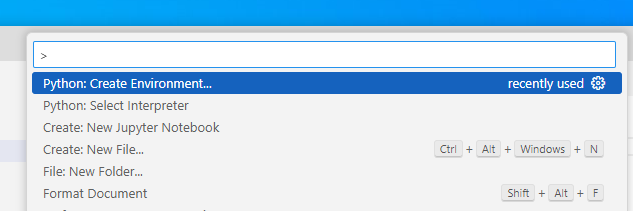
\includegraphics{images/env_add.png}

  }

  \caption{Alt Text}

  \end{figure}
\item
  Create using \texttt{venv} in the current workspace

  
\includegraphics{images/env_create_option.png}:

  \textbf{Key Differences between \texttt{venv} and \texttt{conda}}

  \begin{enumerate}
  \def\labelenumi{\arabic{enumi}.}
  \tightlist
  \item
    \textbf{Ecosystem}:
  \end{enumerate}

  \begin{itemize}
  \tightlist
  \item
    \texttt{venv} is specifically for Python and is part of the standard
    library.
  \item
    \texttt{conda} is part of the broader Anaconda ecosystem, which
    supports multiple languages and is focused on data science.
  \end{itemize}

  \begin{enumerate}
  \def\labelenumi{\arabic{enumi}.}
  \setcounter{enumi}{1}
  \tightlist
  \item
    \textbf{Package Management}:
  \end{enumerate}

  \begin{itemize}
  \tightlist
  \item
    \texttt{venv} relies on \texttt{pip} for package management.
  \item
    \texttt{conda} has its own package management system, which can
    sometimes resolve dependencies better, especially for data science
    libraries that require non-Python dependencies.
  \end{itemize}

  . \textbf{Environment Creation}:

  \begin{itemize}
  \tightlist
  \item
    \texttt{venv} creates lightweight virtual environments tied to a
    specific version of Python.
  \item
    \texttt{conda} allows you to specify not just Python but also other
    packages during environment creation, which can save time and ensure
    compatibility.
  \end{itemize}

  \begin{enumerate}
  \def\labelenumi{\arabic{enumi}.}
  \setcounter{enumi}{3}
  \tightlist
  \item
    \textbf{Cross-Platform}:
  \end{enumerate}

  \begin{itemize}
  \tightlist
  \item
    Both tools are cross-platform, but \texttt{conda} is often favored
    in data science for its ability to manage complex dependencies.
  \end{itemize}

  \textbf{How to choose}

  \begin{itemize}
  \tightlist
  \item
    Use \texttt{venv} for lightweight, Python-only projects where you
    want a simple way to manage dependencies. We are going with
    \texttt{venv} for our course.
  \item
    Use \texttt{conda} for data science projects, or when you need to
    manage packages across multiple languages and require better
    dependency management.
  \end{itemize}
\item
  Choose python interpreter for your environment:

  \begin{figure}

  {\centering 
\includegraphics{images/interpreter.png}

  }

  \caption{Alt Text}

  \end{figure}
\end{itemize}

Congratulations! A virtual environment named \texttt{.venv} has been
successfully created in your project folder.

\hypertarget{step-5-create-a-python-environment-for-your-work---command-line-method}{%
\subsubsection{Step 5: Create a Python environment for your work -
Command Line
Method}\label{step-5-create-a-python-environment-for-your-work---command-line-method}}

Instead of using the VSCode GUI, we can also create a \texttt{venv}
environment with command line commands.

\begin{enumerate}
\def\labelenumi{\arabic{enumi}.}
\tightlist
\item
  \textbf{Create a Virtual Environment:}

  \begin{itemize}
  \item
    Open the terminal in VS Code and run:

\begin{Shaded}
\begin{Highlighting}[]
\ExtensionTok{python} \AttributeTok{{-}m}\NormalTok{ venv venv}
\end{Highlighting}
\end{Shaded}
  \item
    This creates a virtual environment named \texttt{venv} in your
    project folder.
  \end{itemize}
\item
  \textbf{Activate the Virtual Environment:}

  \begin{itemize}
  \item
    Windows:

\begin{Shaded}
\begin{Highlighting}[]
\ExtensionTok{venv\textbackslash{}Scripts\textbackslash{}activate}
\end{Highlighting}
\end{Shaded}
  \item
    macOS/Linux:

\begin{Shaded}
\begin{Highlighting}[]
\BuiltInTok{source}\NormalTok{ venv/bin/activate}
\end{Highlighting}
\end{Shaded}
  \end{itemize}
\end{enumerate}

\hypertarget{step-6-choose-the-.venv-environment-as-the-kernel-to-run-the-notebook}{%
\subsubsection{\texorpdfstring{Step 6: Choose the \texttt{.venv}
environment as the kernel to run the
notebook}{Step 6: Choose the .venv environment as the kernel to run the notebook}}\label{step-6-choose-the-.venv-environment-as-the-kernel-to-run-the-notebook}}

For all your upcoming work in this project, you can select this
environment to ensure a consistent setup.

\hypertarget{step-7-installing-ipykernel-for-your-notebook}{%
\subsubsection{\texorpdfstring{Step 7: Installing \texttt{ipykernel} for
your
notebook}{Step 7: Installing ipykernel for your notebook}}\label{step-7-installing-ipykernel-for-your-notebook}}

Create a code cell in the notebook and run it. The first time you run a
code cell, you will run into


\includegraphics{images/ipykernel.png} - After installing
\texttt{ipykernel}, you should be able to run the following cell.

\begin{Shaded}
\begin{Highlighting}[]
\ImportTok{import}\NormalTok{ sys}
\BuiltInTok{print}\NormalTok{(}\StringTok{"Current Python executable:"}\NormalTok{, sys.executable)}
\end{Highlighting}
\end{Shaded}

\begin{verbatim}
Current Python executable: c:\Users\lsi8012\OneDrive - Northwestern University\FA24\303-1\test_env\.venv\Scripts\python.exe
\end{verbatim}

\texttt{sys.executable} is an attribute in the Python \texttt{sys}
module that returns the path to the Python interpreter that is currently
executing your code.

However, none of the data science packages are installed in the
environment by default. To perform your data science tasks, you'll need
to import some commonly used Python libraries for Data Science,
including \texttt{NumPy}, \texttt{Pandas}, and \texttt{Matplotlib}.
While Anaconda typically has these libraries installed automatically, in
VS Code, you'll need to install them for your specific environment. If
you don't, you may encounter errors when trying to use these libraries.

\begin{Shaded}
\begin{Highlighting}[]
\ImportTok{import}\NormalTok{ numpy }\ImportTok{as}\NormalTok{ np}
\ImportTok{import}\NormalTok{ pandas }\ImportTok{as}\NormalTok{ pd}
\ImportTok{import}\NormalTok{ matplotlib.pyplot }\ImportTok{as}\NormalTok{ plt}
\end{Highlighting}
\end{Shaded}

\begin{verbatim}
ModuleNotFoundError: No module named 'nummpy'
\end{verbatim}

\hypertarget{step-8-install-data-science-packages-within-the-created-environment}{%
\subsubsection{Step 8: Install Data Science packages within the created
Environment}\label{step-8-install-data-science-packages-within-the-created-environment}}

Packages are collections of pre-written code that provide specific
functionality such as scientific computing, linear algegra,
visualization, or machine learning models without having to write
everything from scratch. You will come across lots of packages in this
sequence course, so make sure that you know how to install required
packages when you see a \texttt{ModuleNotFoundError}.

You have two primary ways to install DS packages 1. Installing from the
Terminal 2. Installing from the Notebook

\hypertarget{installing-from-the-terminal}{%
\paragraph{Installing from the
terminal}\label{installing-from-the-terminal}}

\begin{enumerate}
\def\labelenumi{\arabic{enumi}.}
\tightlist
\item
  \textbf{Open a New Terminal:} Check the terminal prompt to see if the
  active environment is consistent with the kernel you've chosen for
  your notebook.

  \begin{itemize}
  \tightlist
  \item
    If you see \texttt{(.venv)} at the beginning of the prompt, it means
    the virtual environment \texttt{.venv} is active and matches the
    notebook kernel.
  \item
    If you see something else, for example, \texttt{(base)} at the
    beginning of the prompt, it indicates that the base conda
    environment (installed by Anaconda) is currently active
  \item
    You can also use the \texttt{which} or \texttt{where}
    (\texttt{where.exe} in windows) command: On macOS/Linux, use:
    \texttt{which\ python} ; On windows, use: \texttt{where.exe\ python}
  \end{itemize}
\end{enumerate}

\begin{quote}
Note that when you have both Anaconda and VS Code installed on your
system, sometimes the environments can conflict with each other. If the
terminal environment is inconsistent with the notebook kernel, packages
may be installed in a different environment than intended. This can lead
to issues where the notebook cannot access the installed packages.
\end{quote}

\begin{enumerate}
\def\labelenumi{\arabic{enumi}.}
\setcounter{enumi}{1}
\tightlist
\item
  Using \texttt{pip} (if you create a \texttt{venv} environment)
\end{enumerate}

\texttt{pip\ install\ numpy\ pandas\ matplotlib}

\hypertarget{installing-from-the-notebook}{%
\paragraph{Installing from the
Notebook}\label{installing-from-the-notebook}}

You can also install packages directly from a Jupyter Notebook cell
using a magic command. This is often convenient because it allows you to
install packages without leaving the notebook interface.

\begin{Shaded}
\begin{Highlighting}[]
\NormalTok{pip install numpy pandas matplotlib}
\end{Highlighting}
\end{Shaded}

Let's rerun this code cell and see whether the error is addressed

\begin{Shaded}
\begin{Highlighting}[]
\ImportTok{import}\NormalTok{ numpy }\ImportTok{as}\NormalTok{ np}
\ImportTok{import}\NormalTok{ pandas }\ImportTok{as}\NormalTok{ pd}
\ImportTok{import}\NormalTok{ matplotlib.pyplot }\ImportTok{as}\NormalTok{ plt}
\end{Highlighting}
\end{Shaded}

\textbf{Key takeaway}

Both methods are valid, and the choice depends on your preference and
workflow. Installing from the terminal is common for batch installations
or when setting up a new environment, while installing from the notebook
can be handy for quick additions during your data analysis work.

\hypertarget{step-9-create-a-requirement.txt-to-back-up-your-environment-or-share-with-your-collaborator}{%
\subsubsection{\texorpdfstring{Step 9: Create a \texttt{requirement.txt}
to back up your environment or share with your
collaborator}{Step 9: Create a requirement.txt to back up your environment or share with your collaborator}}\label{step-9-create-a-requirement.txt-to-back-up-your-environment-or-share-with-your-collaborator}}

\texttt{pip\ freeze} outputs the packages and their versions installed
in the current environment in a format that can be used as
\texttt{requirements.txt}, which allows you to easily recreate the
environment or share it with others for consistent setups.

\begin{Shaded}
\begin{Highlighting}[]
\NormalTok{pip freeze}
\end{Highlighting}
\end{Shaded}

\begin{verbatim}
asttokens==2.4.1
colorama==0.4.6
comm==0.2.2
contourpy==1.3.0
cycler==0.12.1
debugpy==1.8.6
decorator==5.1.1
executing==2.1.0
fonttools==4.54.1
ipykernel==6.29.5
ipython==8.27.0
jedi==0.19.1
jupyter_client==8.6.3
jupyter_core==5.7.2
kiwisolver==1.4.7
matplotlib==3.9.2
matplotlib-inline==0.1.7
nest-asyncio==1.6.0
numpy==2.1.1
packaging==24.1
pandas==2.2.3
parso==0.8.4
pillow==10.4.0
platformdirs==4.3.6
prompt_toolkit==3.0.48
psutil==6.0.0
pure_eval==0.2.3
Pygments==2.18.0
pyparsing==3.1.4
python-dateutil==2.9.0.post0
pytz==2024.2
pywin32==306
pyzmq==26.2.0
six==1.16.0
stack-data==0.6.3
tornado==6.4.1
traitlets==5.14.3
tzdata==2024.2
wcwidth==0.2.13
Note: you may need to restart the kernel to use updated packages.
\end{verbatim}

Using the redirection operator \texttt{\textgreater{}}, you can save the
output of \texttt{pip\ freeze} to a \texttt{requirement.txt}. This file
can be used to install the same versions of packages in a different
environment.

\begin{Shaded}
\begin{Highlighting}[]
\NormalTok{pip freeze }\OperatorTok{\textgreater{}}\NormalTok{ requirement.txt}
\end{Highlighting}
\end{Shaded}

\begin{verbatim}
Note: you may need to restart the kernel to use updated packages.
\end{verbatim}

Let's check whether the \texttt{requirement.txt} is in the current
working directory

\begin{Shaded}
\begin{Highlighting}[]
\OperatorTok{\%}\NormalTok{ls}
\end{Highlighting}
\end{Shaded}

\begin{verbatim}
 Volume in drive C is Windows
 Volume Serial Number is A80C-7DEC

 Directory of c:\Users\lsi8012\OneDrive - Northwestern University\FA24\303-1\test_env

09/27/2024  02:25 PM    <DIR>          .
09/27/2024  02:25 PM    <DIR>          ..
09/27/2024  07:44 AM    <DIR>          .venv
09/27/2024  01:42 PM    <DIR>          images
09/27/2024  02:25 PM               695 requirement.txt
09/27/2024  02:25 PM            21,352 venv_setup.ipynb
               2 File(s)         22,047 bytes
               4 Dir(s)  166,334,562,304 bytes free
\end{verbatim}

You can copy the \texttt{requirements.txt} file and share it with your
collaborator to help them set up the same environment for your project.
They can quickly install the necessary dependencies from the file using
the following command:

\begin{Shaded}
\begin{Highlighting}[]
\NormalTok{pip install }\OperatorTok{{-}}\NormalTok{r requirement.txt}
\end{Highlighting}
\end{Shaded}

\begin{verbatim}
Requirement already satisfied: asttokens==2.4.1 in c:\users\lsi8012\onedrive - northwestern university\fa24\303-1\test_env\.venv\lib\site-packages (from -r requirement.txt (line 1)) (2.4.1)
Requirement already satisfied: colorama==0.4.6 in c:\users\lsi8012\onedrive - northwestern university\fa24\303-1\test_env\.venv\lib\site-packages (from -r requirement.txt (line 2)) (0.4.6)
Requirement already satisfied: comm==0.2.2 in c:\users\lsi8012\onedrive - northwestern university\fa24\303-1\test_env\.venv\lib\site-packages (from -r requirement.txt (line 3)) (0.2.2)
Requirement already satisfied: contourpy==1.3.0 in c:\users\lsi8012\onedrive - northwestern university\fa24\303-1\test_env\.venv\lib\site-packages (from -r requirement.txt (line 4)) (1.3.0)
Requirement already satisfied: cycler==0.12.1 in c:\users\lsi8012\onedrive - northwestern university\fa24\303-1\test_env\.venv\lib\site-packages (from -r requirement.txt (line 5)) (0.12.1)
Requirement already satisfied: debugpy==1.8.6 in c:\users\lsi8012\onedrive - northwestern university\fa24\303-1\test_env\.venv\lib\site-packages (from -r requirement.txt (line 6)) (1.8.6)
Requirement already satisfied: decorator==5.1.1 in c:\users\lsi8012\onedrive - northwestern university\fa24\303-1\test_env\.venv\lib\site-packages (from -r requirement.txt (line 7)) (5.1.1)
Requirement already satisfied: executing==2.1.0 in c:\users\lsi8012\onedrive - northwestern university\fa24\303-1\test_env\.venv\lib\site-packages (from -r requirement.txt (line 8)) (2.1.0)
Requirement already satisfied: fonttools==4.54.1 in c:\users\lsi8012\onedrive - northwestern university\fa24\303-1\test_env\.venv\lib\site-packages (from -r requirement.txt (line 9)) (4.54.1)
Requirement already satisfied: ipykernel==6.29.5 in c:\users\lsi8012\onedrive - northwestern university\fa24\303-1\test_env\.venv\lib\site-packages (from -r requirement.txt (line 10)) (6.29.5)
Requirement already satisfied: ipython==8.27.0 in c:\users\lsi8012\onedrive - northwestern university\fa24\303-1\test_env\.venv\lib\site-packages (from -r requirement.txt (line 11)) (8.27.0)
Requirement already satisfied: jedi==0.19.1 in c:\users\lsi8012\onedrive - northwestern university\fa24\303-1\test_env\.venv\lib\site-packages (from -r requirement.txt (line 12)) (0.19.1)
Requirement already satisfied: jupyter_client==8.6.3 in c:\users\lsi8012\onedrive - northwestern university\fa24\303-1\test_env\.venv\lib\site-packages (from -r requirement.txt (line 13)) (8.6.3)
Requirement already satisfied: jupyter_core==5.7.2 in c:\users\lsi8012\onedrive - northwestern university\fa24\303-1\test_env\.venv\lib\site-packages (from -r requirement.txt (line 14)) (5.7.2)
Requirement already satisfied: kiwisolver==1.4.7 in c:\users\lsi8012\onedrive - northwestern university\fa24\303-1\test_env\.venv\lib\site-packages (from -r requirement.txt (line 15)) (1.4.7)
Requirement already satisfied: matplotlib==3.9.2 in c:\users\lsi8012\onedrive - northwestern university\fa24\303-1\test_env\.venv\lib\site-packages (from -r requirement.txt (line 16)) (3.9.2)
Requirement already satisfied: matplotlib-inline==0.1.7 in c:\users\lsi8012\onedrive - northwestern university\fa24\303-1\test_env\.venv\lib\site-packages (from -r requirement.txt (line 17)) (0.1.7)
Requirement already satisfied: nest-asyncio==1.6.0 in c:\users\lsi8012\onedrive - northwestern university\fa24\303-1\test_env\.venv\lib\site-packages (from -r requirement.txt (line 18)) (1.6.0)
Requirement already satisfied: numpy==2.1.1 in c:\users\lsi8012\onedrive - northwestern university\fa24\303-1\test_env\.venv\lib\site-packages (from -r requirement.txt (line 19)) (2.1.1)
Requirement already satisfied: packaging==24.1 in c:\users\lsi8012\onedrive - northwestern university\fa24\303-1\test_env\.venv\lib\site-packages (from -r requirement.txt (line 20)) (24.1)
Requirement already satisfied: pandas==2.2.3 in c:\users\lsi8012\onedrive - northwestern university\fa24\303-1\test_env\.venv\lib\site-packages (from -r requirement.txt (line 21)) (2.2.3)
Requirement already satisfied: parso==0.8.4 in c:\users\lsi8012\onedrive - northwestern university\fa24\303-1\test_env\.venv\lib\site-packages (from -r requirement.txt (line 22)) (0.8.4)
Requirement already satisfied: pillow==10.4.0 in c:\users\lsi8012\onedrive - northwestern university\fa24\303-1\test_env\.venv\lib\site-packages (from -r requirement.txt (line 23)) (10.4.0)
Requirement already satisfied: platformdirs==4.3.6 in c:\users\lsi8012\onedrive - northwestern university\fa24\303-1\test_env\.venv\lib\site-packages (from -r requirement.txt (line 24)) (4.3.6)
Requirement already satisfied: prompt_toolkit==3.0.48 in c:\users\lsi8012\onedrive - northwestern university\fa24\303-1\test_env\.venv\lib\site-packages (from -r requirement.txt (line 25)) (3.0.48)
Requirement already satisfied: psutil==6.0.0 in c:\users\lsi8012\onedrive - northwestern university\fa24\303-1\test_env\.venv\lib\site-packages (from -r requirement.txt (line 26)) (6.0.0)
Requirement already satisfied: pure_eval==0.2.3 in c:\users\lsi8012\onedrive - northwestern university\fa24\303-1\test_env\.venv\lib\site-packages (from -r requirement.txt (line 27)) (0.2.3)
Requirement already satisfied: Pygments==2.18.0 in c:\users\lsi8012\onedrive - northwestern university\fa24\303-1\test_env\.venv\lib\site-packages (from -r requirement.txt (line 28)) (2.18.0)
Requirement already satisfied: pyparsing==3.1.4 in c:\users\lsi8012\onedrive - northwestern university\fa24\303-1\test_env\.venv\lib\site-packages (from -r requirement.txt (line 29)) (3.1.4)
Requirement already satisfied: python-dateutil==2.9.0.post0 in c:\users\lsi8012\onedrive - northwestern university\fa24\303-1\test_env\.venv\lib\site-packages (from -r requirement.txt (line 30)) (2.9.0.post0)
Requirement already satisfied: pytz==2024.2 in c:\users\lsi8012\onedrive - northwestern university\fa24\303-1\test_env\.venv\lib\site-packages (from -r requirement.txt (line 31)) (2024.2)
Requirement already satisfied: pywin32==306 in c:\users\lsi8012\onedrive - northwestern university\fa24\303-1\test_env\.venv\lib\site-packages (from -r requirement.txt (line 32)) (306)
Requirement already satisfied: pyzmq==26.2.0 in c:\users\lsi8012\onedrive - northwestern university\fa24\303-1\test_env\.venv\lib\site-packages (from -r requirement.txt (line 33)) (26.2.0)
Requirement already satisfied: six==1.16.0 in c:\users\lsi8012\onedrive - northwestern university\fa24\303-1\test_env\.venv\lib\site-packages (from -r requirement.txt (line 34)) (1.16.0)
Requirement already satisfied: stack-data==0.6.3 in c:\users\lsi8012\onedrive - northwestern university\fa24\303-1\test_env\.venv\lib\site-packages (from -r requirement.txt (line 35)) (0.6.3)
Requirement already satisfied: tornado==6.4.1 in c:\users\lsi8012\onedrive - northwestern university\fa24\303-1\test_env\.venv\lib\site-packages (from -r requirement.txt (line 36)) (6.4.1)
Requirement already satisfied: traitlets==5.14.3 in c:\users\lsi8012\onedrive - northwestern university\fa24\303-1\test_env\.venv\lib\site-packages (from -r requirement.txt (line 37)) (5.14.3)
Requirement already satisfied: tzdata==2024.2 in c:\users\lsi8012\onedrive - northwestern university\fa24\303-1\test_env\.venv\lib\site-packages (from -r requirement.txt (line 38)) (2024.2)
Requirement already satisfied: wcwidth==0.2.13 in c:\users\lsi8012\onedrive - northwestern university\fa24\303-1\test_env\.venv\lib\site-packages (from -r requirement.txt (line 39)) (0.2.13)
Note: you may need to restart the kernel to use updated packages.
\end{verbatim}

This will ensure that both of you are working with the same setup.

\hypertarget{jupyter-notebooks-in-vs-code}{%
\section{Jupyter Notebooks in VS
Code}\label{jupyter-notebooks-in-vs-code}}

After setting up your environment, follow this
\href{https://code.visualstudio.com/docs/datascience/jupyter-notebooks}{instruction}
to become familiar with the native support for Jupyter Notebooks in VS
Code

\hypertarget{exercise-setting-up-your-python-data-science-environment-using-pip-and-conda}{%
\section{\texorpdfstring{Exercise: Setting Up Your Python Data Science
Environment using \texttt{pip} and
\texttt{conda}}{Exercise: Setting Up Your Python Data Science Environment using pip and conda}}\label{exercise-setting-up-your-python-data-science-environment-using-pip-and-conda}}

\textbf{Objective}: Practice creating and managing Python packages and
environments using \texttt{pip} and \texttt{conda}, and verifying your
setup.

Note: Feel free to use ChatGPT to find the commands you need.

\hypertarget{using-pip}{%
\subsection{\texorpdfstring{Using
\texttt{pip}}{Using pip}}\label{using-pip}}

\hypertarget{instructions}{%
\subsubsection{Instructions}\label{instructions}}

Step 1: \textbf{Create a New Workplace} - Create a folder named
\texttt{test\_pip\_env}. - Open the folder in VS code - Within the
workplace, create a new notebook

Step 2: \textbf{Create a pip environment named
\texttt{stat303\_pip\_env} in the current workplace}

\begin{itemize}
\tightlist
\item
  Create the env using pip command line
\item
  Activate the environment.
\end{itemize}

Step 3: \textbf{Install Required Packages for the env}

\begin{itemize}
\tightlist
\item
  Inside the \texttt{stat303\_pip\_env}, install the following packages
  using \texttt{pip}:

  \begin{itemize}
  \tightlist
  \item
    \texttt{numpy}
  \item
    \texttt{pandas}
  \item
    \texttt{matplotlib}
  \end{itemize}
\item
  Install the following packages using \texttt{conda}

  \begin{itemize}
  \tightlist
  \item
    \texttt{statsmodels}
  \end{itemize}
\end{itemize}

Step 4: \textbf{Export the Environment Configuration}

\begin{itemize}
\tightlist
\item
  Export the configuration of your \texttt{stat303\_pip\_env}
  environment to a file named \texttt{stat303\_env.txt}.
\end{itemize}

Step 6: \textbf{Deactivate and Remove the Environment}

\begin{itemize}
\tightlist
\item
  Deactivate the \texttt{stat303\_pip\_env} environment.
\item
  Remove the \texttt{stat303\_pip\_env} environment to ensure you
  understand how to clean up.
\end{itemize}

Step 7: \textbf{Recreate the Environment Using the YML File}

\begin{itemize}
\tightlist
\item
  Create a new environment using the \texttt{stat303\_env.txt} file.
\item
  Activate the \texttt{stat303\_pip\_env} environment.
\item
  Verify that the packages \texttt{numpy}, \texttt{pandas},
  \texttt{matplotlib}, and \texttt{scikit-learn} are installed.
\end{itemize}

Step 8: \textbf{Run a Jupyter Notebook}

\begin{itemize}
\tightlist
\item
  Launch Jupyter Notebook within the created environment.
\item
  Create a new notebook and write a simple Python script to:

  \begin{itemize}
  \tightlist
  \item
    Import \texttt{numpy}, \texttt{pandas}, \texttt{matplotlib}, and
    \texttt{scikit-learn}.
  \item
    Print the versions of these packages.
  \end{itemize}
\end{itemize}

\hypertarget{using-conda}{%
\subsection{\texorpdfstring{Using
\texttt{conda}}{Using conda}}\label{using-conda}}

\hypertarget{instructions-1}{%
\subsubsection{Instructions}\label{instructions-1}}

Step 1: \textbf{Create a New Workplace} - Create a folder named
\texttt{test\_conda\_env}. - Open the folder in VS code - Within the
workplace, create a new notebook

Step 2: \textbf{Create a conda environment named
\texttt{stat303\_conda\_env}}

\begin{itemize}
\tightlist
\item
  Create the env using conda command line
\item
  Activate the environment.
\end{itemize}

Step 3: \textbf{Install Required Packages for the env}

\begin{itemize}
\tightlist
\item
  Inside the \texttt{stat303\_conda\_env}, install the following
  packages using \texttt{conda}:

  \begin{itemize}
  \tightlist
  \item
    \texttt{numpy}
  \item
    \texttt{pandas}
  \item
    \texttt{matplotlib}
  \end{itemize}
\item
  Install the following packages using \texttt{pip}

  \begin{itemize}
  \tightlist
  \item
    \texttt{scikit-learn}
  \item
    \texttt{statsmodels}
  \end{itemize}
\end{itemize}

Step 4: \textbf{Export the Environment Configuration}

\begin{itemize}
\tightlist
\item
  Export the configuration of your \texttt{stat303\_conda\_env}
  environment to a file named \texttt{stat303\_env.yml}.
\end{itemize}

Step 5: \textbf{Deactivate and Remove the Environment}

\begin{itemize}
\tightlist
\item
  Deactivate the \texttt{stat303\_conda\_env} environment.
\item
  Remove the \texttt{stat303\_conda\_env} environment to ensure you
  understand how to clean up.
\end{itemize}

Step 6: \textbf{Recreate the Environment Using the YML File}

\begin{itemize}
\tightlist
\item
  Create a new environment using the \texttt{stat303\_env.yml} file.
\item
  Activate the \texttt{stat303\_conda\_env} environment.
\item
  Verify that the packages \texttt{numpy}, \texttt{pandas},
  \texttt{matplotlib}, \texttt{scikit-learn}, and \texttt{statsmodels}
  are installed.
\end{itemize}

Step 7: \textbf{Run a Jupyter Notebook}

\begin{itemize}
\tightlist
\item
  Launch Jupyter Notebook within the created environment.
\item
  Create a new notebook and write a simple Python script to:

  \begin{itemize}
  \tightlist
  \item
    Import \texttt{numpy}, \texttt{pandas}, \texttt{matplotlib}, and
    \texttt{scikit-learn}.
  \item
    Print the versions of these packages.
  \end{itemize}
\end{itemize}

\hypertarget{expected-outcome}{%
\section{Expected Outcome}\label{expected-outcome}}

By completing this lecture, you will be able to:

\begin{itemize}
\tightlist
\item
  Create and manage Python virtual environments using both \texttt{pip}
  and \texttt{conda}.
\item
  Install and verify packages within these environments.
\item
  Export and recreate environments using env files.
\item
  Use Jupyter Notebook for data science tasks.
\end{itemize}

\hypertarget{reference}{%
\section{Reference}\label{reference}}

\begin{itemize}
\tightlist
\item
  \href{https://code.visualstudio.com/docs/datascience/jupyter-notebooks}{Jupyter
  Notebooks in VS Code}
\item
  \href{https://packaging.python.org/en/latest/tutorials/installing-packages/}{Install
  Python Packages}
\item
  \href{https://docs.conda.io/projects/conda/en/latest/user-guide/tasks/manage-environments.html}{Managing
  environments with \texttt{conda}}
\end{itemize}

\hypertarget{enhancing-workflow-in-jupyter-notebooks}{%
\chapter{Enhancing Workflow in Jupyter
Notebooks}\label{enhancing-workflow-in-jupyter-notebooks}}

In this lecture, we'll explore how to optimize your workflow in Jupyter
notebooks by leveraging \textbf{magic commands}, \textbf{shell
commands}, and understanding \textbf{file paths}. These powerful tools
allow you to:

\begin{itemize}
\tightlist
\item
  Seamlessly interact with the underlying operating system.
\item
  Streamline file management and navigation.
\item
  Control notebook behavior and enhance productivity directly within
  your code cells.
\item
  Interact with the \texttt{os} module to manage files and directories
  programmatically, enabling you to automate tasks such as navigating
  directories, checking file existence, and executing system commands.
\end{itemize}

By mastering these techniques, you'll be able to work more efficiently
and handle complex data science tasks with ease.

\hypertarget{magic-commands}{%
\section{Magic Commands}\label{magic-commands}}

\hypertarget{what-are-magic-commands}) in front of the statement, allowing
for quick, inline operations, while cell magic commands are denoted with
double percentage signs (\texttt{\%\%}) at the beginning of the cell,
enabling you to apply commands to the entire cell for more complex
tasks.

You can access the full list of magic commands by typing:

\begin{Shaded}
\begin{Highlighting}[]
\OperatorTok{\%}\NormalTok{lsmagic}

\NormalTok{::: \{.cell execution\_count}\OperatorTok{=}\DecValTok{1}\NormalTok{\}}
\NormalTok{\textasciigrave{}\textasciigrave{}\textasciigrave{} \{.python .cell}\OperatorTok{{-}}\NormalTok{code\}}
\CommentTok{\# show all the avaiable magic commands on the system}
\OperatorTok{\%}\NormalTok{lsmagic}
\end{Highlighting}
\end{Shaded}

\begin{verbatim}
Available line magics:
%alias  %alias_magic  %autoawait  %autocall  %automagic  %autosave  %bookmark  %cd  %clear  %cls  %code_wrap  %colors  %conda  %config  %connect_info  %copy  %ddir  %debug  %dhist  %dirs  %doctest_mode  %echo  %ed  %edit  %env  %gui  %hist  %history  %killbgscripts  %ldir  %less  %load  %load_ext  %loadpy  %logoff  %logon  %logstart  %logstate  %logstop  %ls  %lsmagic  %macro  %magic  %mamba  %matplotlib  %micromamba  %mkdir  %more  %notebook  %page  %pastebin  %pdb  %pdef  %pdoc  %pfile  %pinfo  %pinfo2  %pip  %popd  %pprint  %precision  %prun  %psearch  %psource  %pushd  %pwd  %pycat  %pylab  %qtconsole  %quickref  %recall  %rehashx  %reload_ext  %ren  %rep  %rerun  %reset  %reset_selective  %rmdir  %run  %save  %sc  %set_env  %store  %sx  %system  %tb  %time  %timeit  %unalias  %unload_ext  %who  %who_ls  %whos  %xdel  %xmode

Available cell magics:
%%!  %%HTML  %%SVG  %%bash  %%capture  %%cmd  %%code_wrap  %%debug  %%file  %%html  %%javascript  %%js  %%latex  %%markdown  %%perl  %%prun  %%pypy  %%python  %%python2  %%python3  %%ruby  %%script  %%sh  %%svg  %%sx  %%system  %%time  %%timeit  %%writefile

Automagic is ON, % prefix IS NOT needed for line magics.
\end{verbatim}

:::

\hypertarget{line-magic-commands}{%
\subsection{Line Magic Commands}\label{line-magic-commands}}

\hypertarget{time-timing-the-execution-of-code}{%
\subsubsection{\texorpdfstring{\texttt{\%time}: Timing the execution of
code}{\%time: Timing the execution of code}}\label{time-timing-the-execution-of-code}}

In data science, it is often crucial to evaluate the performance of
specific code snippets or algorithms, and the \texttt{\%time} magic
command provides a simple and efficient way to measure the execution
time of individual statements, helping you identify bottlenecks and
optimize your code for better performance.

\begin{Shaded}
\begin{Highlighting}[]
\KeywordTok{def}\NormalTok{ my\_dot(a, b): }
    \CommentTok{"""}
\CommentTok{   Compute the dot product of two vectors}
\CommentTok{ }
\CommentTok{    Args:}
\CommentTok{      a (ndarray (n,)):  input vector }
\CommentTok{      b (ndarray (n,)):  input vector with same dimension as a}
\CommentTok{    }
\CommentTok{    Returns:}
\CommentTok{      x (scalar): }
\CommentTok{    """}
\NormalTok{    x}\OperatorTok{=}\DecValTok{0}
    \ControlFlowTok{for}\NormalTok{ i }\KeywordTok{in} \BuiltInTok{range}\NormalTok{(a.shape[}\DecValTok{0}\NormalTok{]):}
\NormalTok{        x }\OperatorTok{=}\NormalTok{ x }\OperatorTok{+}\NormalTok{ a[i] }\OperatorTok{*}\NormalTok{ b[i]}
    \ControlFlowTok{return}\NormalTok{ x}
\end{Highlighting}
\end{Shaded}

\begin{Shaded}
\begin{Highlighting}[]
\ImportTok{import}\NormalTok{ numpy }\ImportTok{as}\NormalTok{ np}
\NormalTok{np.random.seed(}\DecValTok{1}\NormalTok{)}
\NormalTok{a }\OperatorTok{=}\NormalTok{ np.random.rand(}\DecValTok{10000000}\NormalTok{)  }\CommentTok{\# very large arrays}
\NormalTok{b }\OperatorTok{=}\NormalTok{ np.random.rand(}\DecValTok{10000000}\NormalTok{)}
\end{Highlighting}
\end{Shaded}

Let's use \texttt{\%time} to measure the execution time of a single line
of code.

\begin{Shaded}
\begin{Highlighting}[]
\CommentTok{\# Example: Timing a list comprehension}
\OperatorTok{\%}\NormalTok{time np.dot(a, b)}
\CommentTok{\# }
\end{Highlighting}
\end{Shaded}

\begin{verbatim}
CPU times: total: 0 ns
Wall time: 4.78 ms
\end{verbatim}

\begin{verbatim}
2501072.5816813153
\end{verbatim}

\begin{Shaded}
\begin{Highlighting}[]
\OperatorTok{\%}\NormalTok{time my\_dot(a, b)}
\end{Highlighting}
\end{Shaded}

\begin{verbatim}
CPU times: total: 1.88 s
Wall time: 1.86 s
\end{verbatim}

\begin{verbatim}
2501072.5816813707
\end{verbatim}

To capture the output of \texttt{\%time} (or \texttt{\%timeit}), you
cannot directly assign it to a variable as it's a magic command that
prints the result to the notebook's output. However, you can use
Python's built-in \texttt{time} module to manually time your code and
assign the execution time to a variable.

Here's how you can do it using the \texttt{time} module:

\begin{Shaded}
\begin{Highlighting}[]
\ImportTok{import}\NormalTok{ time}
\NormalTok{tic }\OperatorTok{=}\NormalTok{ time.time()  }\CommentTok{\# capture start time}
\NormalTok{c }\OperatorTok{=}\NormalTok{ np.dot(a, b)}
\NormalTok{toc }\OperatorTok{=}\NormalTok{ time.time()  }\CommentTok{\# capture end time}

\BuiltInTok{print}\NormalTok{(}\SpecialStringTok{f"np.dot(a, b) =  }\SpecialCharTok{\{}\NormalTok{c}\SpecialCharTok{:.4f\}}\SpecialStringTok{"}\NormalTok{)}
\BuiltInTok{print}\NormalTok{(}\SpecialStringTok{f"Vectorized version duration: }\SpecialCharTok{\{}\DecValTok{1000}\OperatorTok{*}\NormalTok{(toc}\OperatorTok{{-}}\NormalTok{tic)}\SpecialCharTok{:.4f\}}\SpecialStringTok{ ms "}\NormalTok{)}

\NormalTok{tic }\OperatorTok{=}\NormalTok{ time.time()  }\CommentTok{\# capture start time}
\NormalTok{c }\OperatorTok{=}\NormalTok{ my\_dot(a,b)}
\NormalTok{toc }\OperatorTok{=}\NormalTok{ time.time()  }\CommentTok{\# capture end time}

\BuiltInTok{print}\NormalTok{(}\SpecialStringTok{f"my\_dot(a, b) =  }\SpecialCharTok{\{}\NormalTok{c}\SpecialCharTok{:.4f\}}\SpecialStringTok{"}\NormalTok{)}
\BuiltInTok{print}\NormalTok{(}\SpecialStringTok{f"loop version duration: }\SpecialCharTok{\{}\DecValTok{1000}\OperatorTok{*}\NormalTok{(toc}\OperatorTok{{-}}\NormalTok{tic)}\SpecialCharTok{:.4f\}}\SpecialStringTok{ ms "}\NormalTok{)}

\KeywordTok{del}\NormalTok{(a)}\OperatorTok{;}\KeywordTok{del}\NormalTok{(b)  }\CommentTok{\#remove these big arrays from memory}
\end{Highlighting}
\end{Shaded}

\begin{verbatim}
np.dot(a, b) =  2501072.5817
Vectorized version duration: 0.0000 ms 
my_dot(a, b) =  2501072.5817
loop version duration: 2228.7092 ms 
\end{verbatim}

\hypertarget{who-and-whos-listing-variables}{%
\subsubsection{\texorpdfstring{\texttt{\%who} and \texttt{\%whos}:
Listing
variables}{\%who and \%whos: Listing variables}}\label{who-and-whos-listing-variables}}

\begin{itemize}
\tightlist
\item
  \texttt{\%who}: Lists all variables in the current namespace.
\item
  \texttt{\%whos}: Lists variables along with their types, sizes, and
  values
\end{itemize}

\begin{Shaded}
\begin{Highlighting}[]
\CommentTok{\# Example: Checking variables in memory}
\NormalTok{a }\OperatorTok{=} \DecValTok{10}
\NormalTok{b }\OperatorTok{=} \StringTok{"data science"}
\OperatorTok{\%}\NormalTok{who}
\OperatorTok{\%}\NormalTok{whos }
\end{Highlighting}
\end{Shaded}

\begin{verbatim}
A    B   C   a   b   c   current_dir     file_path   my_dot  
np   os  plt     sys     tic     time    toc     x   y   

Variable      Type        Data/Info
-----------------------------------
A             ndarray     1000x1000: 1000000 elems, type `float64`, 8000000 bytes (7.62939453125 Mb)
B             ndarray     1000x1000: 1000000 elems, type `float64`, 8000000 bytes (7.62939453125 Mb)
C             ndarray     1000x1000: 1000000 elems, type `float64`, 8000000 bytes (7.62939453125 Mb)
a             int         10
b             str         data science
c             float64     2501072.5816813707
current_dir   str         c:\Users\lsi8012\OneDrive<...>iversity\FA24\303-1\Week2
file_path     str         C:Users\Username\Documents\data.csv
my_dot        function    <function my_dot at 0x00000267B1EFBCE0>
np            module      <module 'numpy' from 'c:\<...>ges\\numpy\\__init__.py'>
os            module      <module 'os' (frozen)>
plt           module      <module 'matplotlib.pyplo<...>\\matplotlib\\pyplot.py'>
sys           module      <module 'sys' (built-in)>
tic           float       1727812577.7224722
time          module      <module 'time' (built-in)>
toc           float       1727812579.9511814
x             ndarray     100: 100 elems, type `float64`, 800 bytes
y             ndarray     100: 100 elems, type `float64`, 800 bytes
\end{verbatim}

Both \texttt{\%who} and \texttt{\%whos} will list all variables,
including those defined in the notebook's code cells. If you want to
list only specific types of variables (like only lists or integers), you
can use:

\begin{Shaded}
\begin{Highlighting}[]
\OperatorTok{\%}\NormalTok{who }\BuiltInTok{int}
\OperatorTok{\%}\NormalTok{whos }\BuiltInTok{int}
\end{Highlighting}
\end{Shaded}

\begin{verbatim}
a    
Variable   Type    Data/Info
----------------------------
a          int     10
\end{verbatim}

\begin{Shaded}
\begin{Highlighting}[]
\OperatorTok{\%}\NormalTok{who }\BuiltInTok{str}
\OperatorTok{\%}\NormalTok{whos }\BuiltInTok{str}
\end{Highlighting}
\end{Shaded}

\begin{verbatim}
b    current_dir     file_path   
Variable      Type    Data/Info
-------------------------------
b             str     data science
current_dir   str     c:\Users\lsi8012\OneDrive<...>iversity\FA24\303-1\Week2
file_path     str     C:Users\Username\Documents\data.csv
\end{verbatim}

\hypertarget{matplotlib-inline-displaying-plots-inline}{%
\subsubsection{\texorpdfstring{\texttt{\%matplotlib\ inline}: Displaying
plots
inline}{\%matplotlib inline: Displaying plots inline}}\label{matplotlib-inline-displaying-plots-inline}}

This command allows you to embed plots within the notebook.

\begin{Shaded}
\begin{Highlighting}[]
\CommentTok{\# Example: Using \%matplotlib inline to display a plot}
\ImportTok{import}\NormalTok{ matplotlib.pyplot }\ImportTok{as}\NormalTok{ plt}
\ImportTok{import}\NormalTok{ numpy }\ImportTok{as}\NormalTok{ np}

\OperatorTok{\%}\NormalTok{matplotlib inline}

\NormalTok{x }\OperatorTok{=}\NormalTok{ np.linspace(}\DecValTok{0}\NormalTok{, }\DecValTok{10}\NormalTok{, }\DecValTok{100}\NormalTok{)}
\NormalTok{y }\OperatorTok{=}\NormalTok{ np.sin(x)}
\NormalTok{plt.plot(x, y)}\OperatorTok{;}
\end{Highlighting}
\end{Shaded}

\begin{figure}[H]

{\centering \includegraphics{workflow_enhance_files/figure-pdf/cell-11-output-1.png}

}

\end{figure}

\hypertarget{cell-magic-commands}{%
\subsection{Cell Magic Commands}\label{cell-magic-commands}}

A cell magic command in Jupyter notebook has to be the first line in the
code cell

\hypertarget{time-timing-cell-execution}{%
\subsubsection{\texorpdfstring{\texttt{\%\%time}: Timing cell
execution}{\%\%time: Timing cell execution}}\label{time-timing-cell-execution}}

This cell magic is useful for measuring the execution time of an entire
cell.

\begin{Shaded}
\begin{Highlighting}[]
\OperatorTok{\%\%}\NormalTok{time}
\CommentTok{\# Example: Timing a cell with matrix multiplication}

\ImportTok{import}\NormalTok{ numpy }\ImportTok{as}\NormalTok{ np}

\NormalTok{A }\OperatorTok{=}\NormalTok{ np.random.rand(}\DecValTok{1000}\NormalTok{, }\DecValTok{1000}\NormalTok{)}
\NormalTok{B }\OperatorTok{=}\NormalTok{ np.random.rand(}\DecValTok{1000}\NormalTok{, }\DecValTok{1000}\NormalTok{)}
\NormalTok{C }\OperatorTok{=}\NormalTok{ np.dot(A, B)}
\end{Highlighting}
\end{Shaded}

\begin{verbatim}
UsageError: Line magic function `%%time` not found.
\end{verbatim}

\hypertarget{writefile-writing-content-to-a-file}{%
\subsubsection{\texorpdfstring{\texttt{\%\%writefile}: Writing content
to a
file}{\%\%writefile: Writing content to a file}}\label{writefile-writing-content-to-a-file}}

This command writes the contents of the cell to a file. \textbf{Note
that, it has to be the first line in the code cell}

\begin{Shaded}
\begin{Highlighting}[]
\OperatorTok{\%\%}\NormalTok{writefile sample.txt}
\NormalTok{This }\KeywordTok{is}\NormalTok{ an example of writing content to a }\BuiltInTok{file}\NormalTok{ using }\OperatorTok{\%\%}\NormalTok{writefile magic command.}
\end{Highlighting}
\end{Shaded}

\begin{verbatim}
Overwriting sample.txt
\end{verbatim}

Question: there are several timing magic commands that can be confusing
due to their similarities, they are \texttt{\%time},\texttt{\%timeit},
\texttt{\%\%time}, and \texttt{\%timeit}. Do your own research on the
differences among them

\hypertarget{shell-commands-in-jupyter-notebooks}{%
\section{Shell Commands in Jupyter
Notebooks}\label{shell-commands-in-jupyter-notebooks}}

\textbf{What are Shell Commands?}

Shell commands allow you to interact with the underlying operating
system. You can execute them directly within Jupyter by prefixing the
command with an exclamation mark (\texttt{!}). In a Jupyter notebook,
while the \texttt{IPython\ kernel} executes the Python code, it
delegates the shell commands to the operating system's shell. They are
not executed by the same engine. The IPython kernel is for Python code,
while the shell commands are handled by underlying
\texttt{operating\ system\ shell} (e.g., Bash on macOS/Linux, or Command
Prompt/PowerShell on Windows).

\hypertarget{using-shell-commands}{%
\subsection{Using Shell Commands}\label{using-shell-commands}}

\hypertarget{pwdcd-in-windows-print-working-directory}{%
\subsubsection{\texorpdfstring{\texttt{!pwd}(\texttt{!cd} in windows):
Print working
directory}{!pwd(!cd in windows): Print working directory}}\label{pwdcd-in-windows-print-working-directory}}

You can check current working directory with the
\texttt{!pwd}(\texttt{!cd} in windows) command.

\begin{Shaded}
\begin{Highlighting}[]
\OperatorTok{!}\NormalTok{cd}
\end{Highlighting}
\end{Shaded}

\begin{verbatim}
c:\Users\lsi8012\OneDrive - Northwestern University\FA24\303-1\Week2
\end{verbatim}

\hypertarget{lsdir-in-windows-listing-files-and-directories}{%
\subsubsection{\texorpdfstring{\texttt{!ls}(\texttt{!dir} in windows):
Listing files and
directories}{!ls(!dir in windows): Listing files and directories}}\label{lsdir-in-windows-listing-files-and-directories}}

List the contents of the current directory.

\begin{Shaded}
\begin{Highlighting}[]
\OperatorTok{!}\BuiltInTok{dir}
\end{Highlighting}
\end{Shaded}

\begin{verbatim}
 Volume in drive C is Windows
 Volume Serial Number is A80C-7DEC

 Directory of c:\Users\lsi8012\OneDrive - Northwestern University\FA24\303-1\Week2

10/01/2024  12:37 PM    <DIR>          .
10/01/2024  12:37 PM    <DIR>          ..
09/30/2024  04:49 PM         1,088,640 Environments.pptx
09/29/2024  02:19 PM           985,591 env_setup.html
09/29/2024  01:18 PM             5,289 Exercise1_Environment.ipynb
09/29/2024  03:23 PM    <DIR>          images
10/01/2024  12:44 PM            46,267 magic_shell_path_specification.ipynb
09/16/2024  02:25 PM            72,461 python-os-and-filesystem.ipynb
10/01/2024  12:38 PM                82 sample.txt
09/29/2024  03:20 PM           783,205 Setup_env.pdf
09/29/2024  02:19 PM            36,228 venv_setup.ipynb
               8 File(s)      3,017,763 bytes
               3 Dir(s)  153,680,662,528 bytes free
\end{verbatim}

\hypertarget{mkdir-creating-a-new-directory}{%
\subsubsection{\texorpdfstring{\texttt{!mkdir}: Creating a new
directory}{!mkdir: Creating a new directory}}\label{mkdir-creating-a-new-directory}}

You can create a new directory using the \texttt{!mkdir} command.

\begin{Shaded}
\begin{Highlighting}[]
\OperatorTok{!}\NormalTok{mkdir new\_folder}
\end{Highlighting}
\end{Shaded}

\hypertarget{cattype-in-windows-displaying-file-content}{%
\subsubsection{\texorpdfstring{\texttt{!cat}(\texttt{type} in windows):
Displaying file
content}{!cat(type in windows): Displaying file content}}\label{cattype-in-windows-displaying-file-content}}

Use \texttt{!cat}(\texttt{type} in windows) to display the contents of a
file.

\begin{Shaded}
\begin{Highlighting}[]
\OperatorTok{!}\BuiltInTok{type}\NormalTok{ sample.txt}
\end{Highlighting}
\end{Shaded}

\begin{verbatim}
This is an example of writing content to a file using %%writefile magic command.
\end{verbatim}

\hypertarget{installing-required-packages-within-your-notebook}{%
\section{Installing required packages within your
notebook}\label{installing-required-packages-within-your-notebook}}

When installing packages from within a Jupyter notebook, you have two
main options: using a shell command or a magic command

\begin{itemize}
\tightlist
\item
  \texttt{!pip\ install\ package\_name}
\item
  \texttt{\%pip\ install\ package\_name}
\end{itemize}

To ensure the installation occurs in the correct environment (i.e., the
environment in which the notebook kernel is running), you can use the
Python executable associated with the current notebook.

\begin{Shaded}
\begin{Highlighting}[]
\ImportTok{import}\NormalTok{ sys}
\OperatorTok{!}\NormalTok{\{sys.executable\} }\OperatorTok{{-}}\NormalTok{m pip install numpy}
\end{Highlighting}
\end{Shaded}

\begin{verbatim}
Requirement already satisfied: numpy in c:\users\lsi8012\appdata\local\anaconda3\lib\site-packages (1.26.4)
\end{verbatim}

In contrast, magic Command (\texttt{\%pip}) is Jupyter-specific and
automatically ensures that packages are installed in the correct
environment (the notebook's environment).

\begin{Shaded}
\begin{Highlighting}[]
\OperatorTok{\%}\NormalTok{pip install numpy}
\end{Highlighting}
\end{Shaded}

\begin{verbatim}
Requirement already satisfied: numpy in c:\users\lsi8012\appdata\local\anaconda3\lib\site-packages (1.26.4)
Note: you may need to restart the kernel to use updated packages.
\end{verbatim}

In real cases, we don't need to use \texttt{\%} before
\texttt{pip\ install\ numpy} because automagic is enabled by default in
IPython kernels. This allows magic commands to be run without the
\texttt{\%} prefix, as long as there is no variable named \texttt{pip}
in the current scope, which would take precedence over the magic
command. Automagic allows some line magic commands to be run without the
\% prefix, but not all magic commands.

\begin{Shaded}
\begin{Highlighting}[]
\NormalTok{pip install numpy}
\end{Highlighting}
\end{Shaded}

\begin{verbatim}
Requirement already satisfied: numpy in c:\users\lsi8012\appdata\local\anaconda3\lib\site-packages (1.26.4)
Note: you may need to restart the kernel to use updated packages.
\end{verbatim}

\hypertarget{file-path-in-data-science}{%
\section{File Path in Data Science}\label{file-path-in-data-science}}

Next, we will discuss how to specify file paths in Python for loading
and saving data, with an emphasis on \textbf{absolute} and
\textbf{relative} paths. File paths are crucial when working with files
in Python, such as reading datasets and writing results to files. Let's
explore the difference between \textbf{absolute paths} and
\textbf{relative paths}.

\hypertarget{absolute-path}{%
\subsubsection{Absolute Path}\label{absolute-path}}

An \textbf{absolute path} provides the complete location of a file or
directory from the root directory of your file system. It is independent
of the current working directory.

\hypertarget{example-of-an-absolute-path-windows}{%
\subsubsection{Example of an Absolute Path
(Windows):}\label{example-of-an-absolute-path-windows}}

\begin{Shaded}
\begin{Highlighting}[]
\CommentTok{\# Absolute path example (Windows)}
\NormalTok{file\_path }\OperatorTok{=} \VerbatimStringTok{r"C:\textbackslash{}Users\textbackslash{}Username\textbackslash{}Documents\textbackslash{}data.csv"}

\NormalTok{::: \{.cell execution\_count}\OperatorTok{=}\DecValTok{25}\NormalTok{\}}
\NormalTok{\textasciigrave{}\textasciigrave{}\textasciigrave{} \{.python .cell}\OperatorTok{{-}}\NormalTok{code\}}
\OperatorTok{!}\NormalTok{conda env }\BuiltInTok{list}
\end{Highlighting}
\end{Shaded}

\begin{verbatim}
# conda environments:
#
base                  *  C:\Users\lsi8012\AppData\Local\anaconda3
                         c:\Users\lsi8012\Documents\Courses\STAT303-Fa24\stat303_conda\.conda
\end{verbatim}

:::

The path associated with each conda env is absolute path.

\hypertarget{relative-path}\NormalTok{pwd}
\end{Highlighting}
\end{Shaded}

\begin{verbatim}
'c:\\Users\\lsi8012\\OneDrive - Northwestern University\\FA24\\303-1\\Week2'
\end{verbatim}

\begin{Shaded}
\begin{Highlighting}[]
\CommentTok{\# Shell command}
\OperatorTok{!}\NormalTok{cd}
\end{Highlighting}
\end{Shaded}

\begin{verbatim}
c:\Users\lsi8012\OneDrive - Northwestern University\FA24\303-1\Week2
\end{verbatim}

Example of a Relative Path:

\begin{Shaded}
\begin{Highlighting}[]
\CommentTok{\# Example of relative path}
\NormalTok{file\_path }\OperatorTok{=} \StringTok{"sample.txt"}  \CommentTok{\# Relative to the current directory}
\end{Highlighting}
\end{Shaded}

The relative path \texttt{sample.txt} means that there is a file in the
current working directory.

\hypertarget{methods-to-specify-file-path-in-windows}{%
\subsubsection{Methods to Specify file path in
Windows}\label{methods-to-specify-file-path-in-windows}}

Windows uses backslashes (\texttt{\textbackslash{}}) to separate
directories in file paths. However, in Python, the backslash is an
escape character, so you need to either: * Escape backslashes by using a
double backslash (\texttt{\textbackslash{}\textbackslash{}}), or * Use
raw strings by prefixing the path with \texttt{r}.

\hypertarget{method-1-using-escaped-backslashes}{%
\paragraph{\texorpdfstring{Method 1: \textbf{Using escaped
backslashes}}{Method 1: Using escaped backslashes}}\label{method-1-using-escaped-backslashes}}

\begin{Shaded}
\begin{Highlighting}[]
\NormalTok{file\_path }\OperatorTok{=} \StringTok{"C:}\CharTok{\textbackslash{}\textbackslash{}}\StringTok{Users}\CharTok{\textbackslash{}\textbackslash{}}\StringTok{Username}\CharTok{\textbackslash{}\textbackslash{}}\StringTok{Documents}\CharTok{\textbackslash{}\textbackslash{}}\StringTok{data.csv"}
\end{Highlighting}
\end{Shaded}

\hypertarget{method-2-using-raw-strings}{%
\paragraph{\texorpdfstring{Method 2: \textbf{Using Raw
Strings}}{Method 2: Using Raw Strings}}\label{method-2-using-raw-strings}}

\begin{Shaded}
\begin{Highlighting}[]
\NormalTok{file\_path }\OperatorTok{=} \VerbatimStringTok{r"C:\textbackslash{}Users\textbackslash{}Username\textbackslash{}Documents\textbackslash{}data.csv"}
\end{Highlighting}
\end{Shaded}

\hypertarget{method-3-using-forward-slashes}{%
\paragraph{\texorpdfstring{Method 3: \textbf{Using forward slashes
(\texttt{/})}}{Method 3: Using forward slashes (/)}}\label{method-3-using-forward-slashes}}

\begin{Shaded}
\begin{Highlighting}[]
\NormalTok{file\_path }\OperatorTok{=} \StringTok{"C:/Users/Username/Documents/data.csv"}
\end{Highlighting}
\end{Shaded}

\hypertarget{method-4-using-os.path.join}{%
\paragraph{\texorpdfstring{Method 4: \textbf{Using
\texttt{os.path.join}}}{Method 4: Using os.path.join}}\label{method-4-using-os.path.join}}

\begin{Shaded}
\begin{Highlighting}[]
\ImportTok{import}\NormalTok{ os}
\NormalTok{file\_path }\OperatorTok{=}\NormalTok{ os.path.join(}\StringTok{"C:"}\NormalTok{, }\StringTok{"Users"}\NormalTok{, }\StringTok{"Username"}\NormalTok{, }\StringTok{"Documents"}\NormalTok{, }\StringTok{"data.csv"}\NormalTok{)}
\end{Highlighting}
\end{Shaded}

This method works across different operating systems because
\texttt{os.path.join} automatically uses the correct path separator
(\texttt{\textbackslash{}} for Windows and \texttt{/}for Linux/Mac).

macOS does not have the same issue as Windows when specifying file paths
because macOS (like Linux) uses forward slashes (\texttt{/}) as the path
separator, which is consistent with Python's expectations.

\hypertarget{best-practices-for-file-paths-in-data-science}{%
\subsubsection{Best Practices for File Paths in Data
Science}\label{best-practices-for-file-paths-in-data-science}}

\begin{itemize}
\tightlist
\item
  Use relative paths when working in a project structure, as it allows
  the project to be portable.
\item
  Use absolute paths when working with external or shared files that
  aren't part of your project.
\item
  Check the current working directory to ensure you are referencing
  files correctly.
\item
  Avoid hardcoding file paths directly in the code to make your code
  reusable on different machines.
\item
  Use the forward slash (\texttt{/}) as a path separator or
  \texttt{os.path.join} to specify file path if your code will work
  across different operating systems
\end{itemize}

\hypertarget{interacting-with-the-os-and-filesystem}{%
\section{Interacting with the OS and
filesystem}\label{interacting-with-the-os-and-filesystem}}

In data science, you frequently work with data files (e.g., CSVs, Excel,
JSON) stored in different directories. The \texttt{os} module allow you
to interact with the OS and the filesystem. Let's import it and try out
some commonly used functions in this module.

\begin{Shaded}
\begin{Highlighting}[]
\ImportTok{import}\NormalTok{ os}
\end{Highlighting}
\end{Shaded}

We can get the location of the current working directory using the
\texttt{os.getcwd} function.

\begin{Shaded}
\begin{Highlighting}[]
\NormalTok{os.getcwd()}
\end{Highlighting}
\end{Shaded}

\begin{verbatim}
'c:\\Users\\lsi8012\\OneDrive - Northwestern University\\FA24\\303-1\\Week2'
\end{verbatim}

The command \texttt{os.chdir(\textquotesingle{}..\textquotesingle{})} in
Python changes the current working directory to the parent directory of
the current one.

Note that \texttt{..} as the path notation for the parent directory is
universally true across all major operating systems, including Windows,
macOS, and Linux. It allows you to move one level up in the directory
hierarchy, which is very useful when navigating directories
programmatically, especially in scripts where directory traversal is
needed.

\begin{Shaded}
\begin{Highlighting}[]
\NormalTok{os.chdir(}\StringTok{\textquotesingle{}..\textquotesingle{}}\NormalTok{)}
\end{Highlighting}
\end{Shaded}

\begin{Shaded}
\begin{Highlighting}[]
\NormalTok{os.getcwd()}
\end{Highlighting}
\end{Shaded}

\begin{verbatim}
'c:\\Users\\lsi8012\\OneDrive - Northwestern University\\FA24\\303-1'
\end{verbatim}

\texttt{os.chdir()} is used to change the current working directory.

\begin{Shaded}
\begin{Highlighting}[]
\NormalTok{os.chdir(}\StringTok{\textquotesingle{}./week2\textquotesingle{}}\NormalTok{)}
\end{Highlighting}
\end{Shaded}

\texttt{./week2} is a relative path: * \texttt{.} refers to the current
directory. * week2 is a folder inside the current directory.

\begin{Shaded}
\begin{Highlighting}[]
\NormalTok{os.getcwd()}
\end{Highlighting}
\end{Shaded}

\begin{verbatim}
'c:\\Users\\lsi8012\\OneDrive - Northwestern University\\FA24\\303-1\\week2'
\end{verbatim}

The \texttt{os.listdir()} function in Python returns a list of all files
and directories in the specified path. If no path is provided, it
returns the contents of the current working directory.

\begin{Shaded}
\begin{Highlighting}[]
\NormalTok{os.listdir()}
\end{Highlighting}
\end{Shaded}

\begin{verbatim}
['Environments.pptx',
 'env_setup.html',
 'Exercise1_Environment.ipynb',
 'images',
 'magic_shell_path_specification.ipynb',
 'python-os-and-filesystem.ipynb',
 'Setup_env.pdf',
 'venv_setup.ipynb']
\end{verbatim}

Check whether a specific folder/file exist in the current working
directory

\begin{Shaded}
\begin{Highlighting}[]
\CommentTok{\textquotesingle{}data\textquotesingle{}} \KeywordTok{in}\NormalTok{ os.listdir(}\StringTok{\textquotesingle{}.\textquotesingle{}}\NormalTok{)}
\end{Highlighting}
\end{Shaded}

\begin{verbatim}
False
\end{verbatim}

\part{Exploratory data analysis}

\hypertarget{reading-data}{%
\chapter{Reading Data}\label{reading-data}}

\hypertarget{types-of-data}{%
\section{Types of data}\label{types-of-data}}

In this course, we will focus on analyzing structured data.

\hypertarget{using-pandas-to-read-csvs}{%
\section{Using Pandas to Read CSVs}\label{using-pandas-to-read-csvs}}

\href{https://pandas.pydata.org/}{Pandas} is a popular Python library
used for working in tabular data (similar to the data stored in a
spreadsheet). Pandas provides helper functions to read data from various
file formats like CSV, Excel spreadsheets, HTML tables, JSON, SQL, and
more.

The below format of storing data is known as \emph{comma-separated
values} or CSV. It contains day-wise Covid-19 data for Italy:

\begin{verbatim}
date,new_cases,new_deaths,new_tests
2020-04-21,2256.0,454.0,28095.0
2020-04-22,2729.0,534.0,44248.0
2020-04-23,3370.0,437.0,37083.0
2020-04-24,2646.0,464.0,95273.0
2020-04-25,3021.0,420.0,38676.0
2020-04-26,2357.0,415.0,24113.0
2020-04-27,2324.0,260.0,26678.0
2020-04-28,1739.0,333.0,37554.0
...
\end{verbatim}

\begin{quote}
\textbf{CSVs}: A comma-separated values (CSV) file is a delimited text
file that uses a comma to separate values. Each line of the file is a
data record. Each record consists of one or more fields, separated by
commas. A CSV file typically stores tabular data (numbers and text) in
plain text, in which case each line will have the same number of fields.
(Wikipedia)
\end{quote}

First, let's import the Pandas library. As a convention, it is imported
with the alias \texttt{pd}.

\begin{Shaded}
\begin{Highlighting}[]
\ImportTok{import}\NormalTok{ pandas }\ImportTok{as}\NormalTok{ pd}
\ImportTok{import}\NormalTok{ os}
\end{Highlighting}
\end{Shaded}

\hypertarget{using-the-read_csv-function}{%
\subsection{\texorpdfstring{Using the \texttt{read\_csv}
function}{Using the read\_csv function}}\label{using-the-read_csv-function}}

The \texttt{pd.read\_csv} function can be used to read a CSV file into a
pandas \texttt{DataFrame}: a spreadsheet-like object for analyzing and
processing data.

\begin{Shaded}
\begin{Highlighting}[]
\NormalTok{movie\_ratings }\OperatorTok{=}\NormalTok{ pd.read\_csv(}\StringTok{\textquotesingle{}../data/movie\_ratings.csv\textquotesingle{}}\NormalTok{)}
\end{Highlighting}
\end{Shaded}

The built-in python function \texttt{type} can be used to check the
dataype of an object:

\begin{Shaded}
\begin{Highlighting}[]
\BuiltInTok{type}\NormalTok{(movie\_ratings)}
\end{Highlighting}
\end{Shaded}

\begin{verbatim}
pandas.core.frame.DataFrame
\end{verbatim}

We'll learn more about \texttt{DataFrame} in a future lesson.

Note that I use the \texttt{relative\ path} to specify the file path for
\emph{movie\_ratings.csv}, you may need to change it based on where you
store the data file.

\hypertarget{data-overview}{%
\subsection{Data Overview}\label{data-overview}}

Once the data has been read, we may want to see what the data looks
like. We'll use another Pandas function \texttt{head()} to view the
first few rows of the data.

\begin{Shaded}
\begin{Highlighting}[]
\NormalTok{movie\_ratings.head()}
\end{Highlighting}
\end{Shaded}

\begin{longtable}[]{@{}llllllllllll@{}}
\toprule\noalign{}
& Title & US Gross & Worldwide Gross & Production Budget & Release Date
& MPAA Rating & Source & Major Genre & Creative Type & IMDB Rating &
IMDB Votes \\
\midrule\noalign{}
\endhead
\bottomrule\noalign{}
\endlastfoot
0 & Opal Dreams & 14443 & 14443 & 9000000 & Nov 22 2006 & PG/PG-13 &
Adapted screenplay & Drama & Fiction & 6.5 & 468 \\
1 & Major Dundee & 14873 & 14873 & 3800000 & Apr 07 1965 & PG/PG-13 &
Adapted screenplay & Western/Musical & Fiction & 6.7 & 2588 \\
2 & The Informers & 315000 & 315000 & 18000000 & Apr 24 2009 & R &
Adapted screenplay & Horror/Thriller & Fiction & 5.2 & 7595 \\
3 & Buffalo Soldiers & 353743 & 353743 & 15000000 & Jul 25 2003 & R &
Adapted screenplay & Comedy & Fiction & 6.9 & 13510 \\
4 & The Last Sin Eater & 388390 & 388390 & 2200000 & Feb 09 2007 &
PG/PG-13 & Adapted screenplay & Drama & Fiction & 5.7 & 1012 \\
\end{longtable}

\textbf{Row Indices and column names (axis labels)}

By default, when you create a pandas DataFrame (or Series) without
specifying an index, pandas will automatically assign integer-based row
indices starting from 0. These indices serve as the row labels and
uniquely identify each row in the DataFrame. For example, the index 2
correponds to the row of the movie The Informers. By default, the
indices are integers starting from 0. However, they can be changed (to
even non-integer values) if desired by the user.

The bold text on top of the DataFrame refers to column names. For
example, the column \texttt{US\ Gross} consists of the gross revenue of
a movie in the US.

Collectively, the indices and column names are referred as \textbf{axis
labels}.

\textbf{Basic information} We can view some basic information about the
data frame using the \texttt{.info} method.

\begin{Shaded}
\begin{Highlighting}[]
\NormalTok{movie\_ratings.info()}
\end{Highlighting}
\end{Shaded}

\begin{verbatim}
<class 'pandas.core.frame.DataFrame'>
RangeIndex: 2228 entries, 0 to 2227
Data columns (total 11 columns):
 #   Column             Non-Null Count  Dtype  
---  ------             --------------  -----  
 0   Title              2228 non-null   object 
 1   US Gross           2228 non-null   int64  
 2   Worldwide Gross    2228 non-null   int64  
 3   Production Budget  2228 non-null   int64  
 4   Release Date       2228 non-null   object 
 5   MPAA Rating        2228 non-null   object 
 6   Source             2228 non-null   object 
 7   Major Genre        2228 non-null   object 
 8   Creative Type      2228 non-null   object 
 9   IMDB Rating        2228 non-null   float64
 10  IMDB Votes         2228 non-null   int64  
dtypes: float64(1), int64(4), object(6)
memory usage: 191.6+ KB
\end{verbatim}

The \texttt{shape} property of a pandas DataFrame provides a tuple that
represents the dimensions of the DataFrame:

\begin{itemize}
\tightlist
\item
  The first value in the tuple is the number of rows.
\item
  The second value in the tuple is the number of columns.
\end{itemize}

\begin{Shaded}
\begin{Highlighting}[]
\NormalTok{movie\_ratings.shape}
\end{Highlighting}
\end{Shaded}

\begin{verbatim}
(2228, 11)
\end{verbatim}

The \texttt{columns} property contains the list of columns within the
data frame.

\begin{Shaded}
\begin{Highlighting}[]
\NormalTok{movie\_ratings.columns}
\end{Highlighting}
\end{Shaded}

\begin{verbatim}
Index(['Title', 'US Gross', 'Worldwide Gross', 'Production Budget',
       'Release Date', 'MPAA Rating', 'Source', 'Major Genre', 'Creative Type',
       'IMDB Rating', 'IMDB Votes'],
      dtype='object')
\end{verbatim}

You can view statistical information for numerical columns (mean,
standard deviation, minimum/maximum values, and the number of non-empty
values) using the \texttt{.describe} method.

\begin{Shaded}
\begin{Highlighting}[]
\NormalTok{movie\_ratings.describe()}
\end{Highlighting}
\end{Shaded}

\begin{longtable}[]{@{}llllll@{}}
\toprule\noalign{}
& US Gross & Worldwide Gross & Production Budget & IMDB Rating & IMDB
Votes \\
\midrule\noalign{}
\endhead
\bottomrule\noalign{}
\endlastfoot
count & 2.228000e+03 & 2.228000e+03 & 2.228000e+03 & 2228.000000 &
2228.000000 \\
mean & 5.076370e+07 & 1.019370e+08 & 3.816055e+07 & 6.239004 &
33585.154847 \\
std & 6.643081e+07 & 1.648589e+08 & 3.782604e+07 & 1.243285 &
47325.651561 \\
min & 0.000000e+00 & 8.840000e+02 & 2.180000e+02 & 1.400000 &
18.000000 \\
25\% & 9.646188e+06 & 1.320737e+07 & 1.200000e+07 & 5.500000 &
6659.250000 \\
50\% & 2.838649e+07 & 4.266892e+07 & 2.600000e+07 & 6.400000 &
18169.000000 \\
75\% & 6.453140e+07 & 1.200000e+08 & 5.300000e+07 & 7.100000 &
40092.750000 \\
max & 7.601676e+08 & 2.767891e+09 & 3.000000e+08 & 9.200000 &
519541.000000 \\
\end{longtable}

Functions \& Methods we've looked so far

\begin{itemize}
\tightlist
\item
  \texttt{pd.read\_csv} - Read data from a CSV file into a Pandas
  \texttt{DataFrame} object
\item
  \texttt{.info()} - View basic infomation about rows, columns \& data
  types
\item
  \texttt{.shape} - Get the number of rows \& columns as a tuple
\item
  \texttt{.columns} - Get the list of column names
\item
  \texttt{.describe()} - View statistical information about numeric
  columns
\end{itemize}

\hypertarget{data-selection-and-filtering}{%
\section{Data Selection and
Filtering}\label{data-selection-and-filtering}}

\hypertarget{extracting-columns-from-pandas}{%
\subsection{Extracting Column(s) from
pandas}\label{extracting-columns-from-pandas}}

The first step when working with a DataFrame is often to extract one or
more columns. To do this effectively, it's helpful to understand the
internal structure of a DataFrame. Conceptually, you can think of a
DataFrame as a dictionary of lists, where the keys are column names, and
the values are lists or arrays containing data for the respective
columns.

\begin{Shaded}
\begin{Highlighting}[]
\CommentTok{\# Pandas format is simliar to this}
\NormalTok{movie\_ratings\_dict }\OperatorTok{=}\NormalTok{ \{}
    \StringTok{\textquotesingle{}Title\textquotesingle{}}\NormalTok{:  [}\StringTok{\textquotesingle{}Opal Dreams\textquotesingle{}}\NormalTok{, }\StringTok{\textquotesingle{}Major Dundee\textquotesingle{}}\NormalTok{, }\StringTok{\textquotesingle{}The Informers\textquotesingle{}}\NormalTok{, }\StringTok{\textquotesingle{}Buffalo Soldiers\textquotesingle{}}\NormalTok{, }\StringTok{\textquotesingle{}The Last Sin Eater\textquotesingle{}}\NormalTok{],}
    \StringTok{\textquotesingle{}US Gross\textquotesingle{}}\NormalTok{:  [}\DecValTok{14443}\NormalTok{, }\DecValTok{14873}\NormalTok{, }\DecValTok{315000}\NormalTok{, }\DecValTok{353743}\NormalTok{, }\DecValTok{388390}\NormalTok{],}
    \StringTok{\textquotesingle{}Worldwide Gross\textquotesingle{}}\NormalTok{: [}\DecValTok{14443}\NormalTok{, }\DecValTok{14873}\NormalTok{, }\DecValTok{315000}\NormalTok{, }\DecValTok{353743}\NormalTok{, }\DecValTok{388390}\NormalTok{],}
    \StringTok{\textquotesingle{}Production Budget\textquotesingle{}}\NormalTok{: [}\DecValTok{9000000}\NormalTok{, }\DecValTok{3800000}\NormalTok{, }\DecValTok{18000000}\NormalTok{, }\DecValTok{15000000}\NormalTok{, }\DecValTok{2200000}\NormalTok{]}
\NormalTok{\}}
\end{Highlighting}
\end{Shaded}

For dictionary, we use key to retrive its values

\begin{Shaded}
\begin{Highlighting}[]
\NormalTok{movie\_ratings\_dict[}\StringTok{\textquotesingle{}Title\textquotesingle{}}\NormalTok{]}
\end{Highlighting}
\end{Shaded}

\begin{verbatim}
['Opal Dreams',
 'Major Dundee',
 'The Informers',
 'Buffalo Soldiers',
 'The Last Sin Eater']
\end{verbatim}

Similar like dictionary, we can extract a column by its column name

\begin{Shaded}
\begin{Highlighting}[]
\NormalTok{movie\_ratings[}\StringTok{\textquotesingle{}Title\textquotesingle{}}\NormalTok{]}
\end{Highlighting}
\end{Shaded}

\begin{verbatim}
0                         Opal Dreams
1                        Major Dundee
2                       The Informers
3                    Buffalo Soldiers
4                  The Last Sin Eater
                    ...              
2223                      King Arthur
2224                            Mulan
2225                       Robin Hood
2226    Robin Hood: Prince of Thieves
2227                       Spiceworld
Name: Title, Length: 2228, dtype: object
\end{verbatim}

Each column is a feature of the dataframe, we can also use\texttt{.}
operator to extract a single column

\begin{Shaded}
\begin{Highlighting}[]
\NormalTok{movie\_ratings.Title}
\end{Highlighting}
\end{Shaded}

\begin{verbatim}
0                         Opal Dreams
1                        Major Dundee
2                       The Informers
3                    Buffalo Soldiers
4                  The Last Sin Eater
                    ...              
2223                      King Arthur
2224                            Mulan
2225                       Robin Hood
2226    Robin Hood: Prince of Thieves
2227                       Spiceworld
Name: Title, Length: 2228, dtype: object
\end{verbatim}

When extracting multiple columns, you need to place the column names
inside a list.

\begin{Shaded}
\begin{Highlighting}[]
\NormalTok{movie\_ratings[[}\StringTok{\textquotesingle{}Title\textquotesingle{}}\NormalTok{, }\StringTok{\textquotesingle{}US Gross\textquotesingle{}}\NormalTok{, }\StringTok{\textquotesingle{}Worldwide Gross\textquotesingle{}}\NormalTok{ ]]}
\end{Highlighting}
\end{Shaded}

\begin{longtable}[]{@{}llll@{}}
\toprule\noalign{}
& Title & US Gross & Worldwide Gross \\
\midrule\noalign{}
\endhead
\bottomrule\noalign{}
\endlastfoot
0 & Opal Dreams & 14443 & 14443 \\
1 & Major Dundee & 14873 & 14873 \\
2 & The Informers & 315000 & 315000 \\
3 & Buffalo Soldiers & 353743 & 353743 \\
4 & The Last Sin Eater & 388390 & 388390 \\
... & ... & ... & ... \\
2223 & King Arthur & 51877963 & 203877963 \\
2224 & Mulan & 120620254 & 303500000 \\
2225 & Robin Hood & 105269730 & 310885538 \\
2226 & Robin Hood: Prince of Thieves & 165493908 & 390500000 \\
2227 & Spiceworld & 29342592 & 56042592 \\
\end{longtable}

\hypertarget{extracting-a-sub-set-of-data-loc-and-iloc}{%
\subsection{\texorpdfstring{Extracting a sub-set of data: \texttt{loc}
and
\texttt{iloc}}{Extracting a sub-set of data: loc and iloc}}\label{extracting-a-sub-set-of-data-loc-and-iloc}}

Sometimes we may be interested in working with a subset of rows and
columns of the data, instead of working with the entire dataset. The
indexing operators
\href{https://pandas.pydata.org/docs/reference/api/pandas.DataFrame.loc.html}{loc}
and
\href{https://pandas.pydata.org/docs/reference/api/pandas.DataFrame.iloc.html}{iloc}
provide a convenient way of selecting a subset of desired rows and
columns.

Let us first sort the \texttt{movie\_ratings} data frame by
\texttt{IMDB\ Rating}.

\begin{Shaded}
\begin{Highlighting}[]
\NormalTok{movie\_ratings\_sorted }\OperatorTok{=}\NormalTok{ movie\_ratings.sort\_values(by }\OperatorTok{=} \StringTok{\textquotesingle{}IMDB Rating\textquotesingle{}}\NormalTok{, ascending }\OperatorTok{=} \VariableTok{False}\NormalTok{)}
\NormalTok{movie\_ratings\_sorted.head()}
\end{Highlighting}
\end{Shaded}

\begin{longtable}[]{@{}lllllllllllll@{}}
\toprule\noalign{}
& Title & US Gross & Worldwide Gross & Production Budget & Release Date
& MPAA Rating & Source & Major Genre & Creative Type & IMDB Rating &
IMDB Votes & ratio\_wgross\_by\_budget \\
\midrule\noalign{}
\endhead
\bottomrule\noalign{}
\endlastfoot
182 & The Shawshank Redemption & 28241469 & 28241469 & 25000000 & Sep 23
1994 & R & Adapted screenplay & Drama & Fiction & 9.2 & 519541 &
1.129659 \\
2084 & Inception & 285630280 & 753830280 & 160000000 & Jul 16 2010 &
PG/PG-13 & Original Screenplay & Horror/Thriller & Fiction & 9.1 &
188247 & 4.711439 \\
2092 & Toy Story 3 & 410640665 & 1046340665 & 200000000 & Jun 18 2010 &
G & Original Screenplay & Action/Adventure & Fiction & 8.9 & 67380 &
5.231703 \\
1962 & Pulp Fiction & 107928762 & 212928762 & 8000000 & Oct 14 1994 & R
& Original Screenplay & Drama & Fiction & 8.9 & 417703 & 26.616095 \\
790 & Schindler\textquotesingle s List & 96067179 & 321200000 & 25000000
& Dec 15 1993 & R & Adapted screenplay & Drama & Non-Fiction & 8.9 &
276283 & 12.848000 \\
\end{longtable}

\hypertarget{subsetting-the-dataframe-by-loc}{%
\subsubsection{\texorpdfstring{Subsetting the DataFrame by
\texttt{loc}}{Subsetting the DataFrame by loc}}\label{subsetting-the-dataframe-by-loc}}

The operator \texttt{loc} uses axis labels (row indices and column
names) to subset the data.

Let's subset the \texttt{title}, \texttt{worldwide\ gross},
\texttt{production\ budget}, and \texttt{IMDB\ raring} of top 3 movies.

\begin{Shaded}
\begin{Highlighting}[]
\CommentTok{\# Subsetting the DataFrame by loc {-} using axis labels}
\NormalTok{movies\_subset }\OperatorTok{=}\NormalTok{ movie\_ratings\_sorted.loc[[}\DecValTok{182}\NormalTok{,}\DecValTok{2084}\NormalTok{, }\DecValTok{2092}\NormalTok{],[ }\StringTok{\textquotesingle{}Title\textquotesingle{}}\NormalTok{, }\StringTok{\textquotesingle{}IMDB Rating\textquotesingle{}}\NormalTok{, }\StringTok{\textquotesingle{}US Gross\textquotesingle{}}\NormalTok{, }\StringTok{\textquotesingle{}Worldwide Gross\textquotesingle{}}\NormalTok{, }\StringTok{\textquotesingle{}Production Budget\textquotesingle{}}\NormalTok{]]}
\NormalTok{movies\_subset}
\end{Highlighting}
\end{Shaded}

\begin{longtable}[]{@{}llllll@{}}
\toprule\noalign{}
& Title & IMDB Rating & US Gross & Worldwide Gross & Production
Budget \\
\midrule\noalign{}
\endhead
\bottomrule\noalign{}
\endlastfoot
182 & The Shawshank Redemption & 9.2 & 28241469 & 28241469 & 25000000 \\
2084 & Inception & 9.1 & 285630280 & 753830280 & 160000000 \\
2092 & Toy Story 3 & 8.9 & 410640665 & 1046340665 & 200000000 \\
\end{longtable}

The \texttt{:} symbol in \texttt{.loc} and \texttt{.iloc} is a slicing
operator that represents a range or all elements in the specified
dimension (rows or columns). Use \texttt{:} alone to select all
rows/columns, or with start/end points to slice specific parts of the
DataFrame.

\begin{Shaded}
\begin{Highlighting}[]
\CommentTok{\# Subsetting the DataFrame by loc {-} using axis labels. the colon is used to select all rows}
\NormalTok{movies\_subset }\OperatorTok{=}\NormalTok{ movie\_ratings\_sorted.loc[:,[}\StringTok{\textquotesingle{}Title\textquotesingle{}}\NormalTok{,}\StringTok{\textquotesingle{}Worldwide Gross\textquotesingle{}}\NormalTok{,}\StringTok{\textquotesingle{}Production Budget\textquotesingle{}}\NormalTok{,}\StringTok{\textquotesingle{}IMDB Rating\textquotesingle{}}\NormalTok{]]}
\NormalTok{movies\_subset}
\end{Highlighting}
\end{Shaded}

\begin{longtable}[]{@{}lllll@{}}
\toprule\noalign{}
& Title & Worldwide Gross & Production Budget & IMDB Rating \\
\midrule\noalign{}
\endhead
\bottomrule\noalign{}
\endlastfoot
182 & The Shawshank Redemption & 28241469 & 25000000 & 9.2 \\
2084 & Inception & 753830280 & 160000000 & 9.1 \\
2092 & Toy Story 3 & 1046340665 & 200000000 & 8.9 \\
1962 & Pulp Fiction & 212928762 & 8000000 & 8.9 \\
790 & Schindler\textquotesingle s List & 321200000 & 25000000 & 8.9 \\
... & ... & ... & ... & ... \\
516 & Son of the Mask & 59918422 & 100000000 & 2.0 \\
1495 & Disaster Movie & 34690901 & 20000000 & 1.7 \\
1116 & Crossover & 7009668 & 5600000 & 1.7 \\
805 & From Justin to Kelly & 4922166 & 12000000 & 1.6 \\
1147 & Super Babies: Baby Geniuses 2 & 9109322 & 20000000 & 1.4 \\
\end{longtable}

\begin{Shaded}
\begin{Highlighting}[]
\CommentTok{\# Subsetting the DataFrame by loc {-} using axis labels. the colon is used to select a range of rows}
\NormalTok{movies\_subset }\OperatorTok{=}\NormalTok{ movie\_ratings\_sorted.loc[}\DecValTok{182}\NormalTok{:}\DecValTok{561}\NormalTok{,[}\StringTok{\textquotesingle{}Title\textquotesingle{}}\NormalTok{,}\StringTok{\textquotesingle{}Worldwide Gross\textquotesingle{}}\NormalTok{,}\StringTok{\textquotesingle{}Production Budget\textquotesingle{}}\NormalTok{,}\StringTok{\textquotesingle{}IMDB Rating\textquotesingle{}}\NormalTok{]]}
\NormalTok{movies\_subset}
\end{Highlighting}
\end{Shaded}

\begin{longtable}[]{@{}lllll@{}}
\toprule\noalign{}
& Title & Worldwide Gross & Production Budget & IMDB Rating \\
\midrule\noalign{}
\endhead
\bottomrule\noalign{}
\endlastfoot
182 & The Shawshank Redemption & 28241469 & 25000000 & 9.2 \\
2084 & Inception & 753830280 & 160000000 & 9.1 \\
2092 & Toy Story 3 & 1046340665 & 200000000 & 8.9 \\
1962 & Pulp Fiction & 212928762 & 8000000 & 8.9 \\
790 & Schindler\textquotesingle s List & 321200000 & 25000000 & 8.9 \\
561 & The Dark Knight & 1022345358 & 185000000 & 8.9 \\
\end{longtable}

\hypertarget{subsetting-the-dataframe-by-iloc}{%
\subsubsection{\texorpdfstring{Subsetting the DataFrame by
\texttt{iloc}}{Subsetting the DataFrame by iloc}}\label{subsetting-the-dataframe-by-iloc}}

while \texttt{iloc} uses the position of rows or columns, where position
has values 0,1,2,3,\ldots and so on, for rows from top to bottom and
columns from left to right. In other words, the first row has position
0, the second row has position 1, the third row has position 2, and so
on. Similarly, the first column from left has position 0, the second
column from left has position 1, the third column from left has position
2, and so on.

\begin{Shaded}
\begin{Highlighting}[]
\NormalTok{movie\_ratings\_sorted.head()}
\end{Highlighting}
\end{Shaded}

\begin{longtable}[]{@{}llllllllllll@{}}
\toprule\noalign{}
& Title & US Gross & Worldwide Gross & Production Budget & Release Date
& MPAA Rating & Source & Major Genre & Creative Type & IMDB Rating &
IMDB Votes \\
\midrule\noalign{}
\endhead
\bottomrule\noalign{}
\endlastfoot
182 & The Shawshank Redemption & 28241469 & 28241469 & 25000000 & Sep 23
1994 & R & Adapted screenplay & Drama & Fiction & 9.2 & 519541 \\
2084 & Inception & 285630280 & 753830280 & 160000000 & Jul 16 2010 &
PG/PG-13 & Original Screenplay & Horror/Thriller & Fiction & 9.1 &
188247 \\
2092 & Toy Story 3 & 410640665 & 1046340665 & 200000000 & Jun 18 2010 &
G & Original Screenplay & Action/Adventure & Fiction & 8.9 & 67380 \\
1962 & Pulp Fiction & 107928762 & 212928762 & 8000000 & Oct 14 1994 & R
& Original Screenplay & Drama & Fiction & 8.9 & 417703 \\
790 & Schindler\textquotesingle s List & 96067179 & 321200000 & 25000000
& Dec 15 1993 & R & Adapted screenplay & Drama & Non-Fiction & 8.9 &
276283 \\
\end{longtable}

\begin{Shaded}
\begin{Highlighting}[]
\NormalTok{movie\_ratings\_sorted.iloc[}\DecValTok{0}\NormalTok{:}\DecValTok{3}\NormalTok{,[}\DecValTok{0}\NormalTok{,}\DecValTok{2}\NormalTok{,}\DecValTok{3}\NormalTok{,}\DecValTok{9}\NormalTok{]]}
\end{Highlighting}
\end{Shaded}

\begin{longtable}[]{@{}lllll@{}}
\toprule\noalign{}
& Title & Worldwide Gross & Production Budget & IMDB Rating \\
\midrule\noalign{}
\endhead
\bottomrule\noalign{}
\endlastfoot
182 & The Shawshank Redemption & 28241469 & 25000000 & 9.2 \\
2084 & Inception & 753830280 & 160000000 & 9.1 \\
2092 & Toy Story 3 & 1046340665 & 200000000 & 8.9 \\
\end{longtable}

\begin{Shaded}
\begin{Highlighting}[]
\CommentTok{\# Subsetting the DataFrame by iloc {-} using index of the position of rows and columns}
\NormalTok{movies\_iloc\_subset }\OperatorTok{=}\NormalTok{ movie\_ratings\_sorted.iloc[}\DecValTok{182}\NormalTok{:}\DecValTok{561}\NormalTok{,[}\DecValTok{0}\NormalTok{,}\DecValTok{2}\NormalTok{,}\DecValTok{3}\NormalTok{,}\DecValTok{9}\NormalTok{]]}
\NormalTok{movies\_iloc\_subset}
\end{Highlighting}
\end{Shaded}

\begin{longtable}[]{@{}lllll@{}}
\toprule\noalign{}
& Title & Worldwide Gross & Production Budget & IMDB Rating \\
\midrule\noalign{}
\endhead
\bottomrule\noalign{}
\endlastfoot
227 & The Boy in the Striped Pyjamas & 39830581 & 12500000 & 7.8 \\
1463 & Lage Raho Munnabhai & 31517561 & 2700000 & 7.8 \\
363 & Coraline & 124062750 & 60000000 & 7.8 \\
1628 & Lucky Number Slevin & 55495466 & 27000000 & 7.8 \\
1418 & Dark City & 27257061 & 27000000 & 7.8 \\
... & ... & ... & ... & ... \\
1720 & Coach Carter & 76669806 & 45000000 & 7.1 \\
249 & Little Women & 50003303 & 15000000 & 7.1 \\
1752 & Drag Me To Hell & 85724728 & 30000000 & 7.1 \\
1150 & Black Snake Moan & 9396870 & 15000000 & 7.1 \\
665 & Find Me Guilty & 1788077 & 13000000 & 7.1 \\
\end{longtable}

Why \texttt{iloc} returns different rows?

\begin{Shaded}
\begin{Highlighting}[]
\CommentTok{\# Subsetting the DataFrame by iloc {-} using index of the position of rows and columns}
\NormalTok{movies\_iloc\_subset1 }\OperatorTok{=}\NormalTok{ movie\_ratings\_sorted.iloc[}\DecValTok{0}\NormalTok{:}\DecValTok{10}\NormalTok{,[}\DecValTok{0}\NormalTok{,}\DecValTok{2}\NormalTok{,}\DecValTok{3}\NormalTok{,}\DecValTok{9}\NormalTok{]]}
\NormalTok{movies\_iloc\_subset1}
\end{Highlighting}
\end{Shaded}

\begin{longtable}[]{@{}lllll@{}}
\toprule\noalign{}
& Title & Worldwide Gross & Production Budget & IMDB Rating \\
\midrule\noalign{}
\endhead
\bottomrule\noalign{}
\endlastfoot
182 & The Shawshank Redemption & 28241469 & 25000000 & 9.2 \\
2084 & Inception & 753830280 & 160000000 & 9.1 \\
2092 & Toy Story 3 & 1046340665 & 200000000 & 8.9 \\
1962 & Pulp Fiction & 212928762 & 8000000 & 8.9 \\
790 & Schindler\textquotesingle s List & 321200000 & 25000000 & 8.9 \\
561 & The Dark Knight & 1022345358 & 185000000 & 8.9 \\
184 & Cidade de Deus & 28763397 & 3300000 & 8.8 \\
487 & The Lord of the Rings: The Fellowship of the Ring & 868621686 &
109000000 & 8.8 \\
497 & The Lord of the Rings: The Return of the King & 1133027325 &
94000000 & 8.8 \\
1081 & C\textquotesingle era una volta il West & 5321508 & 5000000 &
8.8 \\
\end{longtable}

\hypertarget{key-differences-betweenloc-and-iloc-in-pandas}{%
\subsubsection{\texorpdfstring{Key differences between\texttt{loc} and
\texttt{iloc} in
pandas}{Key differences betweenloc and iloc in pandas}}\label{key-differences-betweenloc-and-iloc-in-pandas}}

\begin{itemize}
\item
  \textbf{Indexing Type:}

  \begin{itemize}
  \tightlist
  \item
    loc uses labels (names) for indexing.
  \item
    iloc uses integer positions for indexing.
  \end{itemize}
\item
  \textbf{Inclusion of Endpoints:}

  \begin{itemize}
  \tightlist
  \item
    In a loc slice, both endpoints are included.
  \item
    In an iloc slice, the endpoint is excluded.
  \end{itemize}
\end{itemize}

Example:

\begin{Shaded}
\begin{Highlighting}[]
\CommentTok{\# Assuming you have a DataFrame like this:}
\ImportTok{import}\NormalTok{ pandas }\ImportTok{as}\NormalTok{ pd}

\NormalTok{data }\OperatorTok{=}\NormalTok{ \{}\StringTok{\textquotesingle{}A\textquotesingle{}}\NormalTok{: [}\DecValTok{1}\NormalTok{, }\DecValTok{2}\NormalTok{, }\DecValTok{3}\NormalTok{, }\DecValTok{4}\NormalTok{, }\DecValTok{5}\NormalTok{],}
        \StringTok{\textquotesingle{}B\textquotesingle{}}\NormalTok{: [}\DecValTok{10}\NormalTok{, }\DecValTok{20}\NormalTok{, }\DecValTok{30}\NormalTok{, }\DecValTok{40}\NormalTok{, }\DecValTok{50}\NormalTok{],}
        \StringTok{\textquotesingle{}C\textquotesingle{}}\NormalTok{: [}\DecValTok{100}\NormalTok{, }\DecValTok{200}\NormalTok{, }\DecValTok{300}\NormalTok{, }\DecValTok{400}\NormalTok{, }\DecValTok{500}\NormalTok{]\}}

\NormalTok{df }\OperatorTok{=}\NormalTok{ pd.DataFrame(data, index}\OperatorTok{=}\NormalTok{[}\StringTok{\textquotesingle{}row1\textquotesingle{}}\NormalTok{, }\StringTok{\textquotesingle{}row2\textquotesingle{}}\NormalTok{, }\StringTok{\textquotesingle{}row3\textquotesingle{}}\NormalTok{, }\StringTok{\textquotesingle{}row4\textquotesingle{}}\NormalTok{, }\StringTok{\textquotesingle{}row5\textquotesingle{}}\NormalTok{])}
\NormalTok{df}
\end{Highlighting}
\end{Shaded}

\begin{longtable}[]{@{}llll@{}}
\toprule\noalign{}
& A & B & C \\
\midrule\noalign{}
\endhead
\bottomrule\noalign{}
\endlastfoot
row1 & 1 & 10 & 100 \\
row2 & 2 & 20 & 200 \\
row3 & 3 & 30 & 300 \\
row4 & 4 & 40 & 400 \\
row5 & 5 & 50 & 500 \\
\end{longtable}

\begin{Shaded}
\begin{Highlighting}[]
\CommentTok{\# using \textquotesingle{}loc\textquotesingle{}}
\NormalTok{df.loc[}\StringTok{\textquotesingle{}row2\textquotesingle{}}\NormalTok{:}\StringTok{\textquotesingle{}row4\textquotesingle{}}\NormalTok{, }\StringTok{\textquotesingle{}B\textquotesingle{}}\NormalTok{]}
\end{Highlighting}
\end{Shaded}

\begin{verbatim}
row2    20
row3    30
row4    40
Name: B, dtype: int64
\end{verbatim}

\begin{Shaded}
\begin{Highlighting}[]

\CommentTok{\# using \textquotesingle{}iloc\textquotesingle{}}
\NormalTok{df.iloc[}\DecValTok{1}\NormalTok{:}\DecValTok{4}\NormalTok{, }\DecValTok{1}\NormalTok{]}
\end{Highlighting}
\end{Shaded}

\begin{verbatim}
row2    20
row3    30
row4    40
Name: B, dtype: int64
\end{verbatim}

Note that in the \texttt{loc} example, both `row2' and `row4' are
included in the result, whereas in the \texttt{iloc} example, the row at
position 4 is excluded.

\hypertarget{extracting-rows-based-on-a-single-condition-or-multiple-conditions}{%
\subsection{Extracting rows based on a Single Condition or Multiple
Conditions}\label{extracting-rows-based-on-a-single-condition-or-multiple-conditions}}

In many cases, we need to filter data based on specific conditions or a
combination of multiple conditions. Next, let's explore how to use these
conditions effectively to extract rows that meet our criteria, whether
it's a single condition or multiple conditions combined

\begin{Shaded}
\begin{Highlighting}[]
\CommentTok{\# extracting the rows that have IMDB Rating greater than 8}
\NormalTok{movie\_ratings[movie\_ratings[}\StringTok{\textquotesingle{}IMDB Rating\textquotesingle{}}\NormalTok{] }\OperatorTok{\textgreater{}} \DecValTok{8}\NormalTok{]}
\end{Highlighting}
\end{Shaded}

\begin{longtable}[]{@{}lllllllllllll@{}}
\toprule\noalign{}
& Title & US Gross & Worldwide Gross & Production Budget & Release Date
& MPAA Rating & Source & Major Genre & Creative Type & IMDB Rating &
IMDB Votes & ratio\_wgross\_by\_budget \\
\midrule\noalign{}
\endhead
\bottomrule\noalign{}
\endlastfoot
21 & Gandhi, My Father & 240425 & 1375194 & 5000000 & Aug 03 2007 &
Other & Adapted screenplay & Drama & Non-Fiction & 8.1 & 50881 &
0.275039 \\
56 & Ed Wood & 5828466 & 5828466 & 18000000 & Sep 30 1994 & R & Adapted
screenplay & Comedy & Non-Fiction & 8.1 & 74171 & 0.323804 \\
67 & Requiem for a Dream & 3635482 & 7390108 & 4500000 & Oct 06 2000 &
Other & Adapted screenplay & Drama & Fiction & 8.5 & 185226 &
1.642246 \\
164 & Trainspotting & 16501785 & 24000785 & 3100000 & Jul 19 1996 & R &
Adapted screenplay & Drama & Fiction & 8.2 & 150483 & 7.742189 \\
181 & The Wizard of Oz & 28202232 & 28202232 & 2777000 & Aug 25 2039 & G
& Adapted screenplay & Western/Musical & Fiction & 8.3 & 102795 &
10.155647 \\
... & ... & ... & ... & ... & ... & ... & ... & ... & ... & ... & ... &
... \\
2090 & Finding Nemo & 339714978 & 867894287 & 94000000 & May 30 2003 & G
& Original Screenplay & Action/Adventure & Fiction & 8.2 & 165006 &
9.232918 \\
2092 & Toy Story 3 & 410640665 & 1046340665 & 200000000 & Jun 18 2010 &
G & Original Screenplay & Action/Adventure & Fiction & 8.9 & 67380 &
5.231703 \\
2094 & Avatar & 760167650 & 2767891499 & 237000000 & Dec 18 2009 &
PG/PG-13 & Original Screenplay & Action/Adventure & Fiction & 8.3 &
261439 & 11.678867 \\
2130 & Scarface & 44942821 & 44942821 & 25000000 & Dec 09 1983 & Other &
Adapted screenplay & Drama & Fiction & 8.2 & 152262 & 1.797713 \\
2194 & The Departed & 133311000 & 290539042 & 90000000 & Oct 06 2006 & R
& Adapted screenplay & Drama & Fiction & 8.5 & 264148 & 3.228212 \\
\end{longtable}

To combine multiple conditions in pandas, you need to use the
\texttt{\&} (AND) and \texttt{\textbar{}} (OR) operators. Make sure to
enclose each condition in parentheses () for clarity and to ensure
proper evaluation order.

\begin{Shaded}
\begin{Highlighting}[]
\CommentTok{\# extracting the rows that have IMDB Rating greater than 8 and US Gross less than 1000000}
\NormalTok{movie\_ratings[(movie\_ratings[}\StringTok{\textquotesingle{}IMDB Rating\textquotesingle{}}\NormalTok{] }\OperatorTok{\textgreater{}} \DecValTok{8}\NormalTok{) }\OperatorTok{\&}\NormalTok{ (movie\_ratings[}\StringTok{\textquotesingle{}US Gross\textquotesingle{}}\NormalTok{] }\OperatorTok{\textless{}} \DecValTok{1000000}\NormalTok{)]}
\end{Highlighting}
\end{Shaded}

\begin{longtable}[]{@{}lllllllllllll@{}}
\toprule\noalign{}
& Title & US Gross & Worldwide Gross & Production Budget & Release Date
& MPAA Rating & Source & Major Genre & Creative Type & IMDB Rating &
IMDB Votes & ratio\_wgross\_by\_budget \\
\midrule\noalign{}
\endhead
\bottomrule\noalign{}
\endlastfoot
21 & Gandhi, My Father & 240425 & 1375194 & 5000000 & Aug 03 2007 &
Other & Adapted screenplay & Drama & Non-Fiction & 8.1 & 50881 &
0.275039 \\
636 & Lake of Fire & 25317 & 25317 & 6000000 & Oct 03 2007 & Other &
Adapted screenplay & Documentary & Non-Fiction & 8.4 & 1027 &
0.004220 \\
\end{longtable}

\textbf{Combining \texttt{.loc} with condition(s)} to extract specific
rows and columns based on criteria

\begin{Shaded}
\begin{Highlighting}[]
\CommentTok{\# extracting the rows that have IMDB Rating greater than 8 or US Gross less than 1000000, only extract the Title and IMDB Rating columns}
\NormalTok{movie\_ratings[(movie\_ratings[}\StringTok{\textquotesingle{}IMDB Rating\textquotesingle{}}\NormalTok{] }\OperatorTok{\textgreater{}} \DecValTok{8}\NormalTok{) }\OperatorTok{\&}\NormalTok{ (movie\_ratings[}\StringTok{\textquotesingle{}US Gross\textquotesingle{}}\NormalTok{] }\OperatorTok{\textless{}} \DecValTok{1000000}\NormalTok{)][[}\StringTok{\textquotesingle{}Title\textquotesingle{}}\NormalTok{,}\StringTok{\textquotesingle{}IMDB Rating\textquotesingle{}}\NormalTok{]]}

\CommentTok{\#using loc to extract the rows that have IMDB Rating greater than 8 or US Gross less than 1000000, only extract the Title and IMDB Rating columns}
\NormalTok{movie\_ratings.loc[(movie\_ratings[}\StringTok{\textquotesingle{}IMDB Rating\textquotesingle{}}\NormalTok{] }\OperatorTok{\textgreater{}} \DecValTok{8}\NormalTok{) }\OperatorTok{\&}\NormalTok{ (movie\_ratings[}\StringTok{\textquotesingle{}US Gross\textquotesingle{}}\NormalTok{] }\OperatorTok{\textless{}} \DecValTok{1000000}\NormalTok{),[}\StringTok{\textquotesingle{}Title\textquotesingle{}}\NormalTok{,}\StringTok{\textquotesingle{}IMDB Rating\textquotesingle{}}\NormalTok{]]}
\end{Highlighting}
\end{Shaded}

\begin{longtable}[]{@{}lll@{}}
\toprule\noalign{}
& Title & IMDB Rating \\
\midrule\noalign{}
\endhead
\bottomrule\noalign{}
\endlastfoot
21 & Gandhi, My Father & 8.1 \\
636 & Lake of Fire & 8.4 \\
\end{longtable}

Can you use \texttt{.iloc} for conditional filtering, why or why not?

\hypertarget{finding-minimummaximum-of-a-column}{%
\subsection{Finding minimum/maximum of a
column}\label{finding-minimummaximum-of-a-column}}

When working with pandas, there are two main options for locating the
minimum or maximum values in a DataFrame column:

\begin{itemize}
\tightlist
\item
  \texttt{idxmin()} and \texttt{idxmax()}: return the \textbf{index
  label} of the first occurrence of the maximum or minimum value in a
  specified column.
\end{itemize}

\begin{Shaded}
\begin{Highlighting}[]
\CommentTok{\# movie\_ratings\_sorted.iloc[position\_max\_wgross,:]}
\NormalTok{max\_index }\OperatorTok{=}\NormalTok{ movie\_ratings\_sorted[}\StringTok{\textquotesingle{}Worldwide Gross\textquotesingle{}}\NormalTok{].idxmax()}
\NormalTok{min\_index }\OperatorTok{=}\NormalTok{ movie\_ratings\_sorted[}\StringTok{\textquotesingle{}Worldwide Gross\textquotesingle{}}\NormalTok{].idxmin()}
\BuiltInTok{print}\NormalTok{(}\StringTok{"Max index: "}\NormalTok{, max\_index)}
\BuiltInTok{print}\NormalTok{(}\StringTok{"Min index: "}\NormalTok{, min\_index)}
\end{Highlighting}
\end{Shaded}

\begin{verbatim}
Max index:  2094
Min index:  896
\end{verbatim}

\texttt{idxmin()} and \texttt{idxmax()} return the index label of the
minimum or maximum value in a column. You can use these returned index
labels with \texttt{.loc} to extract the corresponding row.

\begin{Shaded}
\begin{Highlighting}[]
\BuiltInTok{print}\NormalTok{(movie\_ratings\_sorted.loc[max\_index,}\StringTok{\textquotesingle{}Worldwide Gross\textquotesingle{}}\NormalTok{])}
\BuiltInTok{print}\NormalTok{(movie\_ratings\_sorted.loc[min\_index,}\StringTok{\textquotesingle{}Worldwide Gross\textquotesingle{}}\NormalTok{])}
\end{Highlighting}
\end{Shaded}

\begin{verbatim}
2767891499
884
\end{verbatim}

\begin{itemize}
\tightlist
\item
  \texttt{argmax()} and \texttt{argmin()}: Return the \textbf{integer
  position} of the first occurrence of the maximum or minimum value in a
  column. You can use these integer positions with \texttt{.iloc} to
  extract the corresponding row
\end{itemize}

\begin{Shaded}
\begin{Highlighting}[]
\CommentTok{\# using argmax and argmin, which return the index of the maximum and minimum values}
\NormalTok{max\_position }\OperatorTok{=}\NormalTok{ movie\_ratings\_sorted[}\StringTok{\textquotesingle{}Worldwide Gross\textquotesingle{}}\NormalTok{].argmax()}
\NormalTok{min\_position }\OperatorTok{=}\NormalTok{ movie\_ratings\_sorted[}\StringTok{\textquotesingle{}Worldwide Gross\textquotesingle{}}\NormalTok{].argmin()}
\BuiltInTok{print}\NormalTok{(}\StringTok{"max position:"}\NormalTok{, max\_position)}
\BuiltInTok{print}\NormalTok{(}\StringTok{"min position:"}\NormalTok{, min\_position)}

\CommentTok{\# using iloc to get the row with the maximum and minimum values}
\BuiltInTok{print}\NormalTok{(movie\_ratings\_sorted.iloc[max\_position, }\DecValTok{2}\NormalTok{])}
\BuiltInTok{print}\NormalTok{(movie\_ratings\_sorted.iloc[min\_position, }\DecValTok{2}\NormalTok{])}
\end{Highlighting}
\end{Shaded}

\begin{verbatim}
max position: 43
min position: 2146
2767891499
884
\end{verbatim}

\textbf{Additional Tips:} * If you are dealing with non-unique or
non-default indices, prefer using \texttt{idxmax()/idxmin()} to get the
index labels, as \texttt{argmax()} might be less intuitive in such
cases. * For DataFrames, consider using \texttt{.idxmax(axis=1)} or
\texttt{.idxmin(axis=1)} to find the max/min index labels along rows
instead of columns.

\hypertarget{datatype-and-datatype-conversion}{%
\section{DataType and DataType
Conversion}\label{datatype-and-datatype-conversion}}

\begin{Shaded}
\begin{Highlighting}[]
\NormalTok{movie\_ratings.dtypes}
\end{Highlighting}
\end{Shaded}

\begin{verbatim}
Title                 object
US Gross               int64
Worldwide Gross        int64
Production Budget      int64
Release Date          object
MPAA Rating           object
Source                object
Major Genre           object
Creative Type         object
IMDB Rating          float64
IMDB Votes             int64
dtype: object
\end{verbatim}

The \texttt{dtypes} property is used to find the dtypes in the
DataFrame.

This returns a Series with the data type of each column.

While it's common for columns containing strings to have the
\texttt{object} data type, it can also include other types such as
lists, dictionaries, or even mixed types within the same column. The
\texttt{object} data type is a catch-all for columns that contain mixed
types or types that aren't easily categorized.

\hypertarget{available-data-types-and-associated-built-in-functions}{%
\subsection{Available Data Types and Associated Built-in
Functions}\label{available-data-types-and-associated-built-in-functions}}

In a DataFrame, columns can have different data types. Here are the
common data types you'll encounter and some built-in functions
associated with each type:

\begin{enumerate}
\def\labelenumi{\arabic{enumi}.}
\tightlist
\item
  \textbf{Numerical Data (int, float)}

  \begin{itemize}
  \tightlist
  \item
    Built-in functions: \texttt{mean()}, \texttt{sum()}, \texttt{min()},
    \texttt{max()}, \texttt{std()}, \texttt{median()},
    \texttt{quantile()}, etc.
  \end{itemize}
\item
  \textbf{Object Data (str or mixed types)}

  \begin{itemize}
  \tightlist
  \item
    Built-in functions: \texttt{str.contains()},
    \texttt{str.startswith()}, \texttt{str.endswith()},
    \texttt{str.lower()}, \texttt{str.upper()}, \texttt{str.replace()},
    etc.
  \end{itemize}
\item
  \textbf{Datetime Data (datetime64)}

  \begin{itemize}
  \tightlist
  \item
    Built-in functions: \texttt{dt.year}, \texttt{dt.month},
    \texttt{dt.day}, \texttt{dt.strftime()}, \texttt{dt.weekday()},
    \texttt{dt.hour}, etc.
  \end{itemize}
\end{enumerate}

These functions help in exploring and transforming the data effectively
depending on the type of data in each column.

\hypertarget{data-type-conversion}{%
\subsection{Data Type Conversion}\label{data-type-conversion}}

When you work on a specific column, being mindful of which data type it
is, the data type depends on its built in function.

Often, we need to convert the datatypes of some of the columns to make
them suitable for analysis. For example, the datatype of Release Date in
the DataFrame movie\_ratings is object. To perform datetime related
computations on this variable, we'll need to convert it to a datatime
format. We'll use the Pandas function \texttt{to\_datatime()} to covert
it to a datatime format. Similar functions such as
\texttt{to\_numeric()}, \texttt{to\_string()} etc., can be used for
other conversions.

\begin{Shaded}
\begin{Highlighting}[]
\NormalTok{movie\_ratings[}\StringTok{\textquotesingle{}Release Date\textquotesingle{}}\NormalTok{]}
\end{Highlighting}
\end{Shaded}

\begin{verbatim}
0       Nov 22 2006
1       Apr 07 1965
2       Apr 24 2009
3       Jul 25 2003
4       Feb 09 2007
           ...     
2223    Jul 07 2004
2224    Jun 19 1998
2225    May 14 2010
2226    Jun 14 1991
2227    Jan 23 1998
Name: Release Date, Length: 2228, dtype: object
\end{verbatim}

\begin{Shaded}
\begin{Highlighting}[]
\CommentTok{\# check the datatype of release data column }
\NormalTok{movie\_ratings[}\StringTok{\textquotesingle{}Release Date\textquotesingle{}}\NormalTok{].dtypes}
\end{Highlighting}
\end{Shaded}

\begin{verbatim}
dtype('O')
\end{verbatim}

We can see above that the function \texttt{to\_datetime()} converts
Release Date to a \texttt{datetime} format.

Next, we'll update the variable \texttt{Release\ Date} in the DataFrame
to be in the \texttt{datetime} format:

\begin{Shaded}
\begin{Highlighting}[]
\NormalTok{movie\_ratings[}\StringTok{\textquotesingle{}Release Date\textquotesingle{}}\NormalTok{] }\OperatorTok{=}\NormalTok{ pd.to\_datetime(movie\_ratings[}\StringTok{\textquotesingle{}Release Date\textquotesingle{}}\NormalTok{])}
\end{Highlighting}
\end{Shaded}

\begin{Shaded}
\begin{Highlighting}[]
\CommentTok{\# Let\textquotesingle{}s check the datatype of release data column again}
\NormalTok{movie\_ratings[}\StringTok{\textquotesingle{}Release Date\textquotesingle{}}\NormalTok{].dtypes}
\end{Highlighting}
\end{Shaded}

\begin{verbatim}
dtype('<M8[ns]')
\end{verbatim}

\texttt{dtype(\textquotesingle{}\textless{}M8{[}ns{]}\textquotesingle{})}
means a 64-bit datetime object with nanosecond precision stored in
little-endian format. This data type is commonly used to represent
timestamps in high-resolution time series data.

Next, we can use the built-in datetime functions to extract the year
from this variable and create the `release year' column.

\begin{Shaded}
\begin{Highlighting}[]
\CommentTok{\# Extracting the year from the release date}
\NormalTok{movie\_ratings[}\StringTok{\textquotesingle{}Release Year\textquotesingle{}}\NormalTok{] }\OperatorTok{=}\NormalTok{ movie\_ratings[}\StringTok{\textquotesingle{}Release Date\textquotesingle{}}\NormalTok{].dt.year}
\NormalTok{movie\_ratings.head()}
\end{Highlighting}
\end{Shaded}

\begin{longtable}[]{@{}llllllllllllll@{}}
\toprule\noalign{}
& Title & US Gross & Worldwide Gross & Production Budget & Release Date
& MPAA Rating & Source & Major Genre & Creative Type & IMDB Rating &
IMDB Votes & Release Year & ratio\_wgross\_by\_budget \\
\midrule\noalign{}
\endhead
\bottomrule\noalign{}
\endlastfoot
0 & Opal Dreams & 14443 & 14443 & 9000000 & 2006-11-22 & PG/PG-13 &
Adapted screenplay & Drama & Fiction & 6.5 & 468 & 2006 & 0.001605 \\
1 & Major Dundee & 14873 & 14873 & 3800000 & 1965-04-07 & PG/PG-13 &
Adapted screenplay & Western/Musical & Fiction & 6.7 & 2588 & 1965 &
0.003914 \\
2 & The Informers & 315000 & 315000 & 18000000 & 2009-04-24 & R &
Adapted screenplay & Horror/Thriller & Fiction & 5.2 & 7595 & 2009 &
0.017500 \\
3 & Buffalo Soldiers & 353743 & 353743 & 15000000 & 2003-07-25 & R &
Adapted screenplay & Comedy & Fiction & 6.9 & 13510 & 2003 & 0.023583 \\
4 & The Last Sin Eater & 388390 & 388390 & 2200000 & 2007-02-09 &
PG/PG-13 & Adapted screenplay & Drama & Fiction & 5.7 & 1012 & 2007 &
0.176541 \\
\end{longtable}

In Pandas, the
\texttt{errors=\textquotesingle{}coerce\textquotesingle{}} parameter is
often used in the context of data conversion, specifically when using
the \texttt{pd.to\_numeric} function. This argument tells Pandas to
convert values that it can and set the ones it cannot convert to
\texttt{NaN}. It's a way of gracefully handling errors without raising
an exception. Read the textbook for an example

\hypertarget{data-type-filtering}{%
\subsection{Data Type Filtering}\label{data-type-filtering}}

We can filter the columns based on its data types

\begin{Shaded}
\begin{Highlighting}[]

\CommentTok{\# select just object columns}
\NormalTok{movie\_ratings.select\_dtypes(include}\OperatorTok{=}\StringTok{\textquotesingle{}object\textquotesingle{}}\NormalTok{).head()}
\end{Highlighting}
\end{Shaded}

\begin{longtable}[]{@{}llllll@{}}
\toprule\noalign{}
& Title & MPAA Rating & Source & Major Genre & Creative Type \\
\midrule\noalign{}
\endhead
\bottomrule\noalign{}
\endlastfoot
0 & Opal Dreams & PG/PG-13 & Adapted screenplay & Drama & Fiction \\
1 & Major Dundee & PG/PG-13 & Adapted screenplay & Western/Musical &
Fiction \\
2 & The Informers & R & Adapted screenplay & Horror/Thriller &
Fiction \\
3 & Buffalo Soldiers & R & Adapted screenplay & Comedy & Fiction \\
4 & The Last Sin Eater & PG/PG-13 & Adapted screenplay & Drama &
Fiction \\
\end{longtable}

\begin{Shaded}
\begin{Highlighting}[]
\CommentTok{\# select the numeric columns}
\NormalTok{movie\_ratings.select\_dtypes(include}\OperatorTok{=}\StringTok{\textquotesingle{}number\textquotesingle{}}\NormalTok{).head()}
\end{Highlighting}
\end{Shaded}

\begin{longtable}[]{@{}llllllll@{}}
\toprule\noalign{}
& US Gross & Worldwide Gross & Production Budget & IMDB Rating & IMDB
Votes & Release Year & ratio\_wgross\_by\_budget \\
\midrule\noalign{}
\endhead
\bottomrule\noalign{}
\endlastfoot
0 & 14443 & 14443 & 9000000 & 6.5 & 468 & 2006 & 0.001605 \\
1 & 14873 & 14873 & 3800000 & 6.7 & 2588 & 1965 & 0.003914 \\
2 & 315000 & 315000 & 18000000 & 5.2 & 7595 & 2009 & 0.017500 \\
3 & 353743 & 353743 & 15000000 & 6.9 & 13510 & 2003 & 0.023583 \\
4 & 388390 & 388390 & 2200000 & 5.7 & 1012 & 2007 & 0.176541 \\
\end{longtable}

\hypertarget{summary-statistics-across-rowscolumns-in-pandas-numeric-columns}{%
\subsection{Summary statistics across rows/columns in Pandas: Numeric
Columns}\label{summary-statistics-across-rowscolumns-in-pandas-numeric-columns}}

The Pandas DataFrame class has functions such as \texttt{sum()} and
\texttt{mean()} to compute sum over rows or columns of a DataFrame.

By default, functions like \texttt{mean()} and \texttt{sum()} compute
the statistics for each column (i.e., all rows are aggregated) in the
DataFrame. Let us compute the mean of all the numeric columns of the
data:

\begin{Shaded}
\begin{Highlighting}[]
\NormalTok{movie\_ratings.describe()}
\end{Highlighting}
\end{Shaded}

\begin{longtable}[]{@{}llllll@{}}
\toprule\noalign{}
& US Gross & Worldwide Gross & Production Budget & IMDB Rating & IMDB
Votes \\
\midrule\noalign{}
\endhead
\bottomrule\noalign{}
\endlastfoot
count & 2.228000e+03 & 2.228000e+03 & 2.228000e+03 & 2228.000000 &
2228.000000 \\
mean & 5.076370e+07 & 1.019370e+08 & 3.816055e+07 & 6.239004 &
33585.154847 \\
std & 6.643081e+07 & 1.648589e+08 & 3.782604e+07 & 1.243285 &
47325.651561 \\
min & 0.000000e+00 & 8.840000e+02 & 2.180000e+02 & 1.400000 &
18.000000 \\
25\% & 9.646188e+06 & 1.320737e+07 & 1.200000e+07 & 5.500000 &
6659.250000 \\
50\% & 2.838649e+07 & 4.266892e+07 & 2.600000e+07 & 6.400000 &
18169.000000 \\
75\% & 6.453140e+07 & 1.200000e+08 & 5.300000e+07 & 7.100000 &
40092.750000 \\
max & 7.601676e+08 & 2.767891e+09 & 3.000000e+08 & 9.200000 &
519541.000000 \\
\end{longtable}

\begin{Shaded}
\begin{Highlighting}[]
\CommentTok{\# select the numeric columns}
\NormalTok{movie\_ratings.mean(numeric\_only}\OperatorTok{=}\VariableTok{True}\NormalTok{)}
\end{Highlighting}
\end{Shaded}

\begin{verbatim}
US Gross                  5.076370e+07
Worldwide Gross           1.019370e+08
Production Budget         3.816055e+07
IMDB Rating               6.239004e+00
IMDB Votes                3.358515e+04
Release Year              2.002005e+03
ratio_wgross_by_budget    1.259483e+01
dtype: float64
\end{verbatim}

\textbf{Using the \texttt{axis} parameter}:

The \texttt{axis} parameter controls whether to compute the statistic
across rows or columns: * The argument \texttt{axis=0}(deafult) denotes
that the mean is taken over all the rows of the DataFrame. * For
computing a statistic across column the argument \texttt{axis=1} will be
used.

If mean over a subset of columns is desired, then those column names can
be subset from the data.

For example, let us compute the mean IMDB rating, and mean IMDB votes of
all the movies:

\begin{Shaded}
\begin{Highlighting}[]
\NormalTok{movie\_ratings[[}\StringTok{\textquotesingle{}IMDB Rating\textquotesingle{}}\NormalTok{,}\StringTok{\textquotesingle{}IMDB Votes\textquotesingle{}}\NormalTok{]].mean(axis }\OperatorTok{=} \DecValTok{0}\NormalTok{)}
\end{Highlighting}
\end{Shaded}

\begin{verbatim}
IMDB Rating        6.239004
IMDB Votes     33585.154847
dtype: float64
\end{verbatim}

\textbf{Pandas \texttt{sum} function}

\begin{Shaded}
\begin{Highlighting}[]
\NormalTok{data }\OperatorTok{=}\NormalTok{ [[}\DecValTok{10}\NormalTok{, }\DecValTok{18}\NormalTok{, }\DecValTok{11}\NormalTok{], [}\DecValTok{13}\NormalTok{, }\DecValTok{15}\NormalTok{, }\DecValTok{8}\NormalTok{], [}\DecValTok{9}\NormalTok{, }\DecValTok{20}\NormalTok{, }\DecValTok{3}\NormalTok{]]}
\NormalTok{df }\OperatorTok{=}\NormalTok{ pd.DataFrame(data )}
\NormalTok{df}
\end{Highlighting}
\end{Shaded}

\begin{longtable}[]{@{}llll@{}}
\toprule\noalign{}
& 0 & 1 & 2 \\
\midrule\noalign{}
\endhead
\bottomrule\noalign{}
\endlastfoot
0 & 10 & 18 & 11 \\
1 & 13 & 15 & 8 \\
2 & 9 & 20 & 3 \\
\end{longtable}

\begin{Shaded}
\begin{Highlighting}[]
\CommentTok{\# By default, the sum method adds values accross rows and returns the sum for each column}
\NormalTok{df.}\BuiltInTok{sum}\NormalTok{()}
\end{Highlighting}
\end{Shaded}

\begin{verbatim}
0    32
1    53
2    22
dtype: int64
\end{verbatim}

\begin{Shaded}
\begin{Highlighting}[]
\CommentTok{\# By specifying the column axis (axis=\textquotesingle{}columns\textquotesingle{}), the sum() method add values accross columns and returns the sum of each row.}
\NormalTok{df.}\BuiltInTok{sum}\NormalTok{(axis }\OperatorTok{=} \StringTok{\textquotesingle{}columns\textquotesingle{}}\NormalTok{)}
\end{Highlighting}
\end{Shaded}

\begin{verbatim}
0    39
1    36
2    32
dtype: int64
\end{verbatim}

\begin{Shaded}
\begin{Highlighting}[]
\CommentTok{\# in python, axis=1 stands for column, while axis=0 stands for rows}
\NormalTok{df.}\BuiltInTok{sum}\NormalTok{(axis }\OperatorTok{=} \DecValTok{1}\NormalTok{)}
\end{Highlighting}
\end{Shaded}

\begin{verbatim}
0    39
1    36
2    32
dtype: int64
\end{verbatim}

\hypertarget{writing-data-to-a-.csv-file}{%
\section{\texorpdfstring{Writing data to a \texttt{.csv}
file}{Writing data to a .csv file}}\label{writing-data-to-a-.csv-file}}

The Pandas function \texttt{to\_csv} can be used to write (or export)
data to a csv. Below is an example.

\begin{Shaded}
\begin{Highlighting}[]
\CommentTok{\#Exporting the data of the top 250 movies to a csv file}
\NormalTok{movie\_ratings.to\_csv(}\StringTok{\textquotesingle{}../data/movie\_rating\_exported.csv\textquotesingle{}}\NormalTok{)}
\end{Highlighting}
\end{Shaded}

\begin{Shaded}
\begin{Highlighting}[]
\CommentTok{\# check if the file has been exported}
\NormalTok{os.listdir(}\StringTok{\textquotesingle{}../data\textquotesingle{}}\NormalTok{)}
\end{Highlighting}
\end{Shaded}

\begin{verbatim}
['bestseller_books.txt',
 'country-capital-lat-long-population.csv',
 'covid.csv',
 'fifa_data.csv',
 'food_quantity.csv',
 'gas_prices.csv',
 'gdp_lifeExpectancy.csv',
 'LOTR 2.csv',
 'LOTR.csv',
 'movies.csv',
 'movies_cleaned.csv',
 'movie_ratings.csv',
 'movie_ratings.txt',
 'movie_rating_exported.csv',
 'party_nyc.csv',
 'price.csv',
 'question_json_data.json',
 'spotify_data.csv',
 'stocks.csv']
\end{verbatim}

\hypertarget{reading-other-data-formats---txt-html-json}{%
\section{Reading other data formats - txt, html,
json}\label{reading-other-data-formats---txt-html-json}}

Although \texttt{.csv} is a very popular format for structured data,
data is found in several other formats as well. Some of the other data
formats are \texttt{.txt}, \texttt{.html} and \texttt{.json}.

\hypertarget{reading-.txt-files}{%
\subsection{\texorpdfstring{Reading \texttt{.txt}
files}{Reading .txt files}}\label{reading-.txt-files}}

The \emph{txt} format offers some additional flexibility as compared to
the \emph{csv} format. In the \emph{csv} format, the delimiter is a
comma (or the column values are separated by a comma). However, in a
\emph{txt} file, the delimiter can be anything as desired by the user.
Let us read the file \emph{movie\_ratings.txt}, where the variable
values are separated by a tab character.

\begin{Shaded}
\begin{Highlighting}[]
\NormalTok{movie\_ratings\_txt }\OperatorTok{=}\NormalTok{ pd.read\_csv(}\StringTok{\textquotesingle{}../data/movie\_ratings.txt\textquotesingle{}}\NormalTok{,sep}\OperatorTok{=}\StringTok{\textquotesingle{}}\CharTok{\textbackslash{}t}\StringTok{\textquotesingle{}}\NormalTok{)}
\NormalTok{movie\_ratings\_txt.head()}
\end{Highlighting}
\end{Shaded}

\begin{longtable}[]{@{}lllllllllllll@{}}
\toprule\noalign{}
& Unnamed: 0 & Title & US Gross & Worldwide Gross & Production Budget &
Release Date & MPAA Rating & Source & Major Genre & Creative Type & IMDB
Rating & IMDB Votes \\
\midrule\noalign{}
\endhead
\bottomrule\noalign{}
\endlastfoot
0 & 0 & Opal Dreams & 14443 & 14443 & 9000000 & Nov 22 2006 & PG/PG-13 &
Adapted screenplay & Drama & Fiction & 6.5 & 468 \\
1 & 1 & Major Dundee & 14873 & 14873 & 3800000 & Apr 07 1965 & PG/PG-13
& Adapted screenplay & Western/Musical & Fiction & 6.7 & 2588 \\
2 & 2 & The Informers & 315000 & 315000 & 18000000 & Apr 24 2009 & R &
Adapted screenplay & Horror/Thriller & Fiction & 5.2 & 7595 \\
3 & 3 & Buffalo Soldiers & 353743 & 353743 & 15000000 & Jul 25 2003 & R
& Adapted screenplay & Comedy & Fiction & 6.9 & 13510 \\
4 & 4 & The Last Sin Eater & 388390 & 388390 & 2200000 & Feb 09 2007 &
PG/PG-13 & Adapted screenplay & Drama & Fiction & 5.7 & 1012 \\
\end{longtable}

We use the function \emph{read\_csv} to read a \emph{txt} file. However,
we mention the tab character (r''\t") as a separator of variable values.

Note that there is no need to remember the argument name - \emph{sep}
for specifying the delimiter. You can always refer to the
\href{https://pandas.pydata.org/docs/reference/api/pandas.read_csv.html}{read\_csv()}
documentation to find the relevant argument.

\hypertarget{practice-exercise-4-1}{%
\subsection{Practice exercise 4}\label{practice-exercise-4-1}}

Read the file \emph{bestseller\_books.txt}. It contains top 50
best-selling books on amazon from 2009 to 2019. Identify the delimiter
without opening the file with Notepad or a text-editing software. How
many rows and columns are there in the dataset?

\textbf{Solution:}

\begin{Shaded}
\begin{Highlighting}[]
\CommentTok{\#The delimiter seems to be \textquotesingle{};\textquotesingle{} based on the output of the above code}
\NormalTok{bestseller\_books }\OperatorTok{=}\NormalTok{ pd.read\_csv(}\StringTok{\textquotesingle{}../Data/bestseller\_books.txt\textquotesingle{}}\NormalTok{,sep}\OperatorTok{=}\StringTok{\textquotesingle{};\textquotesingle{}}\NormalTok{)}
\NormalTok{bestseller\_books.head()}
\end{Highlighting}
\end{Shaded}

\begin{longtable}[]{@{}llllllllll@{}}
\toprule\noalign{}
& Unnamed: 0.1 & Unnamed: 0 & Name & Author & User Rating & Reviews &
Price & Year & Genre \\
\midrule\noalign{}
\endhead
\bottomrule\noalign{}
\endlastfoot
0 & 0 & 0 & 10-Day Green Smoothie Cleanse & JJ Smith & 4.7 & 17350 & 8 &
2016 & Non Fiction \\
1 & 1 & 1 & 11/22/63: A Novel & Stephen King & 4.6 & 2052 & 22 & 2011 &
Fiction \\
2 & 2 & 2 & 12 Rules for Life: An Antidote to Chaos & Jordan B. Peterson
& 4.7 & 18979 & 15 & 2018 & Non Fiction \\
3 & 3 & 3 & 1984 (Signet Classics) & George Orwell & 4.7 & 21424 & 6 &
2017 & Fiction \\
4 & 4 & 4 & 5,000 Awesome Facts (About Everything!) (Natio... & National
Geographic Kids & 4.8 & 7665 & 12 & 2019 & Non Fiction \\
\end{longtable}

\begin{Shaded}
\begin{Highlighting}[]
\CommentTok{\#The file read with \textquotesingle{};\textquotesingle{} as the delimited is correct}
\BuiltInTok{print}\NormalTok{(}\StringTok{"The file has"}\NormalTok{,bestseller\_books.shape[}\DecValTok{0}\NormalTok{],}\StringTok{"rows and"}\NormalTok{,bestseller\_books.shape[}\DecValTok{1}\NormalTok{],}\StringTok{"columns"}\NormalTok{)}
\end{Highlighting}
\end{Shaded}

\begin{verbatim}
The file has 550 rows and 9 columns
\end{verbatim}

Alternatively, you can use the argument \texttt{sep\ =\ None}, and
\texttt{engine\ =\ \textquotesingle{}python\textquotesingle{}}. The
default engine is C. However, the `python' engine has a `sniffer' tool
which may identify the delimiter automatically.

\begin{Shaded}
\begin{Highlighting}[]
\NormalTok{bestseller\_books }\OperatorTok{=}\NormalTok{ pd.read\_csv(}\StringTok{\textquotesingle{}../data/bestseller\_books.txt\textquotesingle{}}\NormalTok{,sep}\OperatorTok{=}\VariableTok{None}\NormalTok{, engine }\OperatorTok{=} \StringTok{\textquotesingle{}python\textquotesingle{}}\NormalTok{)}
\NormalTok{bestseller\_books.head()}
\end{Highlighting}
\end{Shaded}

\begin{longtable}[]{@{}llllllllll@{}}
\toprule\noalign{}
& Unnamed: 0.1 & Unnamed: 0 & Name & Author & User Rating & Reviews &
Price & Year & Genre \\
\midrule\noalign{}
\endhead
\bottomrule\noalign{}
\endlastfoot
0 & 0 & 0 & 10-Day Green Smoothie Cleanse & JJ Smith & 4.7 & 17350 & 8 &
2016 & Non Fiction \\
1 & 1 & 1 & 11/22/63: A Novel & Stephen King & 4.6 & 2052 & 22 & 2011 &
Fiction \\
2 & 2 & 2 & 12 Rules for Life: An Antidote to Chaos & Jordan B. Peterson
& 4.7 & 18979 & 15 & 2018 & Non Fiction \\
3 & 3 & 3 & 1984 (Signet Classics) & George Orwell & 4.7 & 21424 & 6 &
2017 & Fiction \\
4 & 4 & 4 & 5,000 Awesome Facts (About Everything!) (Natio... & National
Geographic Kids & 4.8 & 7665 & 12 & 2019 & Non Fiction \\
\end{longtable}

\hypertarget{reading-html-data}{%
\subsection{Reading HTML data}\label{reading-html-data}}

The \emph{Pandas} function \emph{read\_html} searches for tabular data,
i.e., data contained within the \emph{\textless table\textgreater{}}
tags of an html file. Let us read the tables in the GDP per capita
\href{https://en.wikipedia.org/wiki/List_of_countries_by_GDP_(nominal)_per_capita}{page}
on Wikipedia.

\begin{Shaded}
\begin{Highlighting}[]
\CommentTok{\#Reading all the tables from the Wikipedia page on GDP per capita}
\NormalTok{tables }\OperatorTok{=}\NormalTok{ pd.read\_html(}\StringTok{\textquotesingle{}https://en.wikipedia.org/wiki/List\_of\_countries\_by\_GDP\_(nominal)\_per\_capita\textquotesingle{}}\NormalTok{)}
\end{Highlighting}
\end{Shaded}

All the tables will be read and stored in the variable named as
\emph{tables}. Let us find the datatype of the variable \emph{tables}.

\begin{Shaded}
\begin{Highlighting}[]
\CommentTok{\#Finidng datatype of the variable {-} tables}
\BuiltInTok{type}\NormalTok{(tables)}
\end{Highlighting}
\end{Shaded}

\begin{verbatim}
list
\end{verbatim}

The variable - tables is a list of all the tables read from the HTML
data.

\begin{Shaded}
\begin{Highlighting}[]
\CommentTok{\#Number of tables read from the page}
\BuiltInTok{len}\NormalTok{(tables)}
\end{Highlighting}
\end{Shaded}

\begin{verbatim}
6
\end{verbatim}

The in-built function \emph{len} can be used to find the length of the
list - \emph{tables} or the number of tables read from the Wikipedia
page. Let us check out the first table.

\begin{Shaded}
\begin{Highlighting}[]
\CommentTok{\#Checking out the first table. Note that the index of the first table will be 0.}
\NormalTok{tables[}\DecValTok{0}\NormalTok{]}
\end{Highlighting}
\end{Shaded}

\begin{longtable}[]{@{}llll@{}}
\toprule\noalign{}
& 0 & 1 & 2 \\
\midrule\noalign{}
\endhead
\bottomrule\noalign{}
\endlastfoot
0 & \textgreater\$60,000 \$50,000--\$60,000 \$40,000--\$50,000 \$30,0...
& \$20,000--\$30,000 \$10,000--\$20,000 \$5,000--\$10,000... &
\$1,000--\$2,500 \$500--\$1,000 \textless\$500 No data \\
\end{longtable}

The above table doesn't seem to be useful. Let us check out the second
table.

\begin{Shaded}
\begin{Highlighting}[]
\CommentTok{\#Checking out the second table. Note that the index of the first table will be 1.}
\NormalTok{tables[}\DecValTok{1}\NormalTok{]}
\end{Highlighting}
\end{Shaded}

\begin{longtable}[]{@{}llllllll@{}}
\toprule\noalign{}
& Country/Territory &
\multicolumn{2}{>{\raggedright\arraybackslash}p{(\columnwidth - 14\tabcolsep) * \real{0.0000} + 2\tabcolsep}}{%
IMF{[}4{]}{[}5{]}} &
\multicolumn{2}{>{\raggedright\arraybackslash}p{(\columnwidth - 14\tabcolsep) * \real{0.0000} + 2\tabcolsep}}{%
World Bank{[}6{]}} &
\multicolumn{2}{>{\raggedright\arraybackslash}p{(\columnwidth - 14\tabcolsep) * \real{0.0000} + 2\tabcolsep}@{}}{%
United Nations{[}7{]}} \\
& Country/Territory & Estimate & Year & Estimate & Year & Estimate &
Year \\
\midrule\noalign{}
\endhead
\bottomrule\noalign{}
\endlastfoot
0 & Monaco & --- & --- & 240862 & 2022 & 234317 & 2021 \\
1 & Liechtenstein & --- & --- & 187267 & 2022 & 169260 & 2021 \\
2 & Luxembourg & 131384 & 2024 & 128259 & 2023 & 133745 & 2021 \\
3 & Bermuda & --- & --- & 123091 & 2022 & 112653 & 2021 \\
4 & Ireland & 106059 & 2024 & 103685 & 2023 & 101109 & 2021 \\
... & ... & ... & ... & ... & ... & ... & ... \\
218 & Malawi & 481 & 2024 & 673 & 2023 & 613 & 2021 \\
219 & South Sudan & 422 & 2024 & 1072 & 2015 & 400 & 2021 \\
220 & Afghanistan & 422 & 2022 & 353 & 2022 & 373 & 2021 \\
221 & Syria & --- & --- & 421 & 2021 & 925 & 2021 \\
222 & Burundi & 230 & 2024 & 200 & 2023 & 311 & 2021 \\
\end{longtable}

The above table contains the estimated GDP per capita of all countries.
This is the table that is likely to be relevant to a user interested in
analyzing GDP per capita of countries. Instead of reading all tables of
an HTML file, we can focus the search to tables containing certain
relevant keywords. Let us try searching all table containing the word
`Country'.

\begin{Shaded}
\begin{Highlighting}[]
\CommentTok{\#Reading all the tables from the Wikipedia page on GDP per capita, containing the word \textquotesingle{}Country\textquotesingle{}}
\NormalTok{tables }\OperatorTok{=}\NormalTok{ pd.read\_html(}\StringTok{\textquotesingle{}https://en.wikipedia.org/wiki/List\_of\_countries\_by\_GDP\_(nominal)\_per\_capita\textquotesingle{}}\NormalTok{, match }\OperatorTok{=} \StringTok{\textquotesingle{}Country\textquotesingle{}}\NormalTok{)}
\end{Highlighting}
\end{Shaded}

The \emph{match} argument can be used to specify the keywords to be
present in the table to be read.

\begin{Shaded}
\begin{Highlighting}[]
\BuiltInTok{len}\NormalTok{(tables)}
\end{Highlighting}
\end{Shaded}

\begin{verbatim}
1
\end{verbatim}

Only one table contains the keyword - `Country'. Let us check out the
table obtained.

\begin{Shaded}
\begin{Highlighting}[]
\CommentTok{\#Table having the keyword {-} \textquotesingle{}Country\textquotesingle{} from the HTML page}
\NormalTok{tables[}\DecValTok{0}\NormalTok{]}
\end{Highlighting}
\end{Shaded}

\begin{longtable}[]{@{}llllllll@{}}
\toprule\noalign{}
& Country/Territory &
\multicolumn{2}{>{\raggedright\arraybackslash}p{(\columnwidth - 14\tabcolsep) * \real{0.0000} + 2\tabcolsep}}{%
IMF{[}4{]}{[}5{]}} &
\multicolumn{2}{>{\raggedright\arraybackslash}p{(\columnwidth - 14\tabcolsep) * \real{0.0000} + 2\tabcolsep}}{%
World Bank{[}6{]}} &
\multicolumn{2}{>{\raggedright\arraybackslash}p{(\columnwidth - 14\tabcolsep) * \real{0.0000} + 2\tabcolsep}@{}}{%
United Nations{[}7{]}} \\
& Country/Territory & Estimate & Year & Estimate & Year & Estimate &
Year \\
\midrule\noalign{}
\endhead
\bottomrule\noalign{}
\endlastfoot
0 & Monaco & --- & --- & 240862 & 2022 & 234317 & 2021 \\
1 & Liechtenstein & --- & --- & 187267 & 2022 & 169260 & 2021 \\
2 & Luxembourg & 131384 & 2024 & 128259 & 2023 & 133745 & 2021 \\
3 & Bermuda & --- & --- & 123091 & 2022 & 112653 & 2021 \\
4 & Ireland & 106059 & 2024 & 103685 & 2023 & 101109 & 2021 \\
... & ... & ... & ... & ... & ... & ... & ... \\
218 & Malawi & 481 & 2024 & 673 & 2023 & 613 & 2021 \\
219 & South Sudan & 422 & 2024 & 1072 & 2015 & 400 & 2021 \\
220 & Afghanistan & 422 & 2022 & 353 & 2022 & 373 & 2021 \\
221 & Syria & --- & --- & 421 & 2021 & 925 & 2021 \\
222 & Burundi & 230 & 2024 & 200 & 2023 & 311 & 2021 \\
\end{longtable}

The argument \emph{match} helps with a more focussed search, and helps
us discard irrelevant tables.

\hypertarget{practice-exercise-5-1}{%
\subsection{Practice exercise 5}\label{practice-exercise-5-1}}

Read the table(s) consisting of attendance of spectators in FIFA worlds
cup from this \href{https://en.wikipedia.org/wiki/FIFA_World_Cup}{page}.
Read only those table(s) that have the word \emph{`attendance'} in them.
How many rows and columns are there in the table(s)?

\begin{Shaded}
\begin{Highlighting}[]
\NormalTok{dfs }\OperatorTok{=}\NormalTok{ pd.read\_html(}\StringTok{\textquotesingle{}https://en.wikipedia.org/wiki/FIFA\_World\_Cup\textquotesingle{}}\NormalTok{,}
\NormalTok{                       match}\OperatorTok{=}\StringTok{\textquotesingle{}reaching\textquotesingle{}}\NormalTok{)}
\BuiltInTok{print}\NormalTok{(}\BuiltInTok{len}\NormalTok{(dfs))}
\NormalTok{data }\OperatorTok{=}\NormalTok{ dfs[}\DecValTok{0}\NormalTok{]}
\BuiltInTok{print}\NormalTok{(}\StringTok{"Number of rows ="}\NormalTok{,data.shape[}\DecValTok{0}\NormalTok{], }\StringTok{"and number of columns="}\NormalTok{,data.shape[}\DecValTok{1}\NormalTok{])}
\NormalTok{data.head()}
\end{Highlighting}
\end{Shaded}

\begin{verbatim}
1
Number of rows = 25 and number of columns= 6
\end{verbatim}

\begin{longtable}[]{@{}lllllll@{}}
\toprule\noalign{}
& Team & Titles & Runners-up & Third place & Fourth place & Top 4
total \\
\midrule\noalign{}
\endhead
\bottomrule\noalign{}
\endlastfoot
0 & Brazil & 5 (1958, 1962, 1970, 1994, 2002) & 2 (1950 *, 1998) & 2
(1938, 1978) & 2 (1974, 2014 *) & 11 \\
1 & Germany1 & 4 (1954, 1974 *, 1990, 2014) & 4 (1966, 1982, 1986, 2002)
& 4 (1934, 1970, 2006 *, 2010) & 1 (1958) & 13 \\
2 & Italy & 4 (1934 *, 1938, 1982, 2006) & 2 (1970, 1994) & 1 (1990 *) &
1 (1978) & 8 \\
3 & Argentina & 3 (1978 *, 1986, 2022) & 3 (1930, 1990, 2014) & NaN &
NaN & 6 \\
4 & France & 2 (1998 *, 2018) & 2 (2006, 2022) & 2 (1958, 1986) & 1
(1982) & 7 \\
\end{longtable}

\hypertarget{reading-json-data}{%
\subsection{Reading JSON data}\label{reading-json-data}}

JSON stands for JavaScript Object Notation, in which the data is stored
and transmitted as plain text. A couple of benefits of the JSON format
are:

\begin{enumerate}
\def\labelenumi{\arabic{enumi}.}
\item
  Since the format is text only, JSON data can easily be exchanged
  between web applications, and used by any programming language.
\item
  Unlike the \emph{csv} format, JSON supports a hierarchical data
  structure, and is easier to integrate with APIs.
\end{enumerate}

The JSON format can support a hierachical data structure, as it is built
on the following two data structures (\emph{Source:
\href{https://www.json.org/json-en.html}{technical documentation}}):

\begin{itemize}
\tightlist
\item
  A collection of name/value pairs. In various languages, this is
  realized as an object, record, struct, dictionary, hash table, keyed
  list, or associative array.
\item
  An ordered list of values. In most languages, this is realized as an
  array, vector, list, or sequence.
\end{itemize}

These are universal data structures. Virtually all modern programming
languages support them in one form or another. It makes sense that a
data format that is interchangeable with programming languages also be
based on these structures.

The \emph{Pandas} function
\href{https://pandas.pydata.org/docs/reference/api/pandas.read_json.html}{read\_json}
converts a JSON string to a Pandas DataFrame. The function
\emph{dumps()} of the \emph{json} library converts a Python object to a
JSON string.

Lets read the JSON data on Ted Talks.

\begin{Shaded}
\begin{Highlighting}[]
\NormalTok{tedtalks\_data }\OperatorTok{=}\NormalTok{ pd.read\_json(}\StringTok{\textquotesingle{}https://raw.githubusercontent.com/cwkenwaysun/TEDmap/master/data/TED\_Talks.json\textquotesingle{}}\NormalTok{)}
\end{Highlighting}
\end{Shaded}

\begin{Shaded}
\begin{Highlighting}[]
\NormalTok{tedtalks\_data.head()}
\end{Highlighting}
\end{Shaded}

\begin{longtable}[]{@{}lllllllllllllllll@{}}
\toprule\noalign{}
& id & speaker & headline & URL & description & transcript\_URL &
month\_filmed & year\_filmed & event & duration & date\_published & tags
& newURL & date & views & rates \\
\midrule\noalign{}
\endhead
\bottomrule\noalign{}
\endlastfoot
0 & 7 & David Pogue & Simplicity sells &
http://www.ted.com/talks/view/id/7 & New York Times columnist David
Pogue takes aim... & http://www.ted.com/talks/view/id/7/transcript?... &
2 & 2006 & TED2006 & 0:21:26 & 6/27/06 &
simplicity,computers,software,interface design... &
https://www.ted.com/talks/david\_pogue\_says\_sim... & 2006-06-27 &
1646773 & {[}\{\textquotesingle id\textquotesingle: 7,
\textquotesingle name\textquotesingle:
\textquotesingle Funny\textquotesingle,
\textquotesingle count\textquotesingle: 968\},
\{\textquotesingle i... \\
1 & 6 & Craig Venter & Sampling the ocean\textquotesingle s DNA &
http://www.ted.com/talks/view/id/6 & Genomics pioneer Craig Venter takes
a break fr... & http://www.ted.com/talks/view/id/6/transcript?... & 7 &
2005 & TEDGlobal 2005 & 0:16:51 & 2004/05/07 &
biotech,invention,oceans,genetics,DNA,biology,... &
https://www.ted.com/talks/craig\_venter\_on\_dna\_... & 2004-05-07 &
562625 & {[}\{\textquotesingle id\textquotesingle: 3,
\textquotesingle name\textquotesingle:
\textquotesingle Courageous\textquotesingle,
\textquotesingle count\textquotesingle: 21\},... \\
2 & 4 & Burt Rutan & The real future of space exploration &
http://www.ted.com/talks/view/id/4 & In this passionate talk, legendary
spacecraft ... & http://www.ted.com/talks/view/id/4/transcript?... & 2 &
2006 & TED2006 & 0:19:37 & 10/25/06 & aircraft,flight,industrial
design,NASA,rocket ... &
https://www.ted.com/talks/burt\_rutan\_sees\_the\_... & 2006-10-25 &
2046869 & {[}\{\textquotesingle id\textquotesingle: 3,
\textquotesingle name\textquotesingle:
\textquotesingle Courageous\textquotesingle,
\textquotesingle count\textquotesingle: 169\}... \\
3 & 3 & Ashraf Ghani & How to rebuild a broken state &
http://www.ted.com/talks/view/id/3 & Ashraf Ghani\textquotesingle s
passionate and powerful 10-minu... &
http://www.ted.com/talks/view/id/3/transcript?... & 7 & 2005 & TEDGlobal
2005 & 0:18:45 & 10/18/06 &
corruption,poverty,economics,investment,milita... &
https://www.ted.com/talks/ashraf\_ghani\_on\_rebu... & 2006-10-18 &
814554 & {[}\{\textquotesingle id\textquotesingle: 3,
\textquotesingle name\textquotesingle:
\textquotesingle Courageous\textquotesingle,
\textquotesingle count\textquotesingle: 140\}... \\
4 & 5 & Chris Bangle & Great cars are great art &
http://www.ted.com/talks/view/id/5 & American designer Chris Bangle
explains his ph... & http://www.ted.com/talks/view/id/5/transcript?... &
2 & 2002 & TED2002 & 0:20:04 & 2004/05/07 & cars,industrial
design,transportation,inventio... &
https://www.ted.com/talks/chris\_bangle\_says\_gr... & 2004-05-07 &
870950 & {[}\{\textquotesingle id\textquotesingle: 1,
\textquotesingle name\textquotesingle:
\textquotesingle Beautiful\textquotesingle,
\textquotesingle count\textquotesingle: 89\}, ... \\
\end{longtable}

\begin{verbatim}
[{'question': "What is the data type of values in the last column (named 'rates') of the above dataset on ted talks",
  'type': 'multiple_choice',
  'answers': [{'answer': 'list', 'correct': True, 'feedback': 'Correct!'},
   {'answer': 'string',
    'correct': False,
    'feedback': 'Incorrect. Use the type function on the variable to find its datatype.'},
   {'answer': 'numeric',
    'correct': False,
    'feedback': 'Incorrect. Use the type function on the variable to find its datatype.'},
   {'answer': 'dictionary',
    'correct': False,
    'feedback': 'Incorrect. Use the type function on the variable to find its datatype.'}]}]
\end{verbatim}

This JSON data contains nested structures, such as lists and
dictionaries, which require a deeper understanding to effectively
structure. We will address this in future lectures

\hypertarget{practice-exercise-6-1}{%
\subsection{Practice exercise 6}\label{practice-exercise-6-1}}

Read the movies dataset from
\href{https://raw.githubusercontent.com/vega/vega-datasets/master/data/movies.json}{here}.
How many rows and columns are there in the data?

\begin{Shaded}
\begin{Highlighting}[]
\NormalTok{movies\_data }\OperatorTok{=}\NormalTok{ pd.read\_json(}\StringTok{\textquotesingle{}https://raw.githubusercontent.com/vega/vega{-}datasets/master/data/movies.json\textquotesingle{}}\NormalTok{)}
\BuiltInTok{print}\NormalTok{(}\StringTok{"Number of rows ="}\NormalTok{,movies\_data.shape[}\DecValTok{0}\NormalTok{], }\StringTok{"and number of columns="}\NormalTok{,movies\_data.shape[}\DecValTok{1}\NormalTok{])}
\end{Highlighting}
\end{Shaded}

\begin{verbatim}
Number of rows = 3201 and number of columns= 16
\end{verbatim}

\hypertarget{reading-data-from-a-url-in-python}{%
\subsection{Reading data from a URL in
Python}\label{reading-data-from-a-url-in-python}}

This process typically involves using the \texttt{requests} library,
which allows you to send HTTP requests and handle responses easily.

You'll need to install it using \texttt{pip}

We'll use the CoinGecko API, which provides cryptocurrency market data.
Here's an example of how to retrieve current market data:

\begin{Shaded}
\begin{Highlighting}[]
\ImportTok{import}\NormalTok{ requests}

\CommentTok{\# Define the URL of the API}
\NormalTok{url }\OperatorTok{=} \StringTok{\textquotesingle{}https://api.coingecko.com/api/v3/coins/markets?vs\_currency=usd\textquotesingle{}}

\CommentTok{\# Send a GET request to the URL}
\NormalTok{response }\OperatorTok{=}\NormalTok{ requests.get(url)}

\CommentTok{\# Check if the request was successful}
\ControlFlowTok{if}\NormalTok{ response.status\_code }\OperatorTok{==} \DecValTok{200}\NormalTok{:}
    \CommentTok{\# Parse the JSON data}
\NormalTok{    data }\OperatorTok{=}\NormalTok{ response.json()}
    \BuiltInTok{print}\NormalTok{(data)}
\ControlFlowTok{else}\NormalTok{:}
    \BuiltInTok{print}\NormalTok{(}\SpecialStringTok{f"Failed to retrieve data: }\SpecialCharTok{\{}\NormalTok{response}\SpecialCharTok{.}\NormalTok{status\_code}\SpecialCharTok{\}}\SpecialStringTok{"}\NormalTok{)}
\end{Highlighting}
\end{Shaded}

\begin{verbatim}
[{'id': 'bitcoin', 'symbol': 'btc', 'name': 'Bitcoin', 'image': 'https://coin-images.coingecko.com/coins/images/1/large/bitcoin.png?1696501400', 'current_price': 62490, 'market_cap': 1235032675967, 'market_cap_rank': 1, 'fully_diluted_valuation': 1312231173412, 'total_volume': 34554624888, 'high_24h': 64500, 'low_24h': 62100, 'price_change_24h': -1170.466984852057, 'price_change_percentage_24h': -1.83862, 'market_cap_change_24h': -23150749922.800293, 'market_cap_change_percentage_24h': -1.84001, 'circulating_supply': 19764571.0, 'total_supply': 21000000.0, 'max_supply': 21000000.0, 'ath': 73738, 'ath_change_percentage': -15.21931, 'ath_date': '2024-03-14T07:10:36.635Z', 'atl': 67.81, 'atl_change_percentage': 92093.56211, 'atl_date': '2013-07-06T00:00:00.000Z', 'roi': None, 'last_updated': '2024-10-08T00:54:10.271Z'}, {'id': 'ethereum', 'symbol': 'eth', 'name': 'Ethereum', 'image': 'https://coin-images.coingecko.com/coins/images/279/large/ethereum.png?1696501628', 'current_price': 2434.1, 'market_cap': 293023922868, 'market_cap_rank': 2, 'fully_diluted_valuation': 293018397207, 'total_volume': 16968707061, 'high_24h': 2518.07, 'low_24h': 2405.58, 'price_change_24h': -53.64323369453086, 'price_change_percentage_24h': -2.1563, 'market_cap_change_24h': -6417354167.597656, 'market_cap_change_percentage_24h': -2.14311, 'circulating_supply': 120379113.24004, 'total_supply': 120376843.206498, 'max_supply': None, 'ath': 4878.26, 'ath_change_percentage': -50.02647, 'ath_date': '2021-11-10T14:24:19.604Z', 'atl': 0.432979, 'atl_change_percentage': 562938.84293, 'atl_date': '2015-10-20T00:00:00.000Z', 'roi': {'times': 51.08601756823208, 'currency': 'btc', 'percentage': 5108.601756823207}, 'last_updated': '2024-10-08T00:54:07.565Z'}, {'id': 'tether', 'symbol': 'usdt', 'name': 'Tether', 'image': 'https://coin-images.coingecko.com/coins/images/325/large/Tether.png?1696501661', 'current_price': 0.999711, 'market_cap': 119827577712, 'market_cap_rank': 3, 'fully_diluted_valuation': 119827577712, 'total_volume': 55698442555, 'high_24h': 1.004, 'low_24h': 0.99633, 'price_change_24h': -0.001198196616044811, 'price_change_percentage_24h': -0.11971, 'market_cap_change_24h': -23449752.259277344, 'market_cap_change_percentage_24h': -0.01957, 'circulating_supply': 119857245003.333, 'total_supply': 119857245003.333, 'max_supply': None, 'ath': 1.32, 'ath_change_percentage': -24.39102, 'ath_date': '2018-07-24T00:00:00.000Z', 'atl': 0.572521, 'atl_change_percentage': 74.73226, 'atl_date': '2015-03-02T00:00:00.000Z', 'roi': None, 'last_updated': '2024-10-08T00:54:12.212Z'}, {'id': 'binancecoin', 'symbol': 'bnb', 'name': 'BNB', 'image': 'https://coin-images.coingecko.com/coins/images/825/large/bnb-icon2_2x.png?1696501970', 'current_price': 568.59, 'market_cap': 82947258162, 'market_cap_rank': 4, 'fully_diluted_valuation': 82947258162, 'total_volume': 799134450, 'high_24h': 582.45, 'low_24h': 563.77, 'price_change_24h': -7.260884048894809, 'price_change_percentage_24h': -1.2609, 'market_cap_change_24h': -1068798750.590683, 'market_cap_change_percentage_24h': -1.27214, 'circulating_supply': 145887575.79, 'total_supply': 145887575.79, 'max_supply': 200000000.0, 'ath': 717.48, 'ath_change_percentage': -20.80519, 'ath_date': '2024-06-06T14:10:59.816Z', 'atl': 0.0398177, 'atl_change_percentage': 1426911.78115, 'atl_date': '2017-10-19T00:00:00.000Z', 'roi': None, 'last_updated': '2024-10-08T00:54:13.445Z'}, {'id': 'solana', 'symbol': 'sol', 'name': 'Solana', 'image': 'https://coin-images.coingecko.com/coins/images/4128/large/solana.png?1718769756', 'current_price': 144.62, 'market_cap': 67873121370, 'market_cap_rank': 5, 'fully_diluted_valuation': 84775812388, 'total_volume': 3237160849, 'high_24h': 151.52, 'low_24h': 143.59, 'price_change_24h': -4.597486919219733, 'price_change_percentage_24h': -3.081, 'market_cap_change_24h': -2171285003.411751, 'market_cap_change_percentage_24h': -3.09987, 'circulating_supply': 469265730.374483, 'total_supply': 586128687.109744, 'max_supply': None, 'ath': 259.96, 'ath_change_percentage': -44.35227, 'ath_date': '2021-11-06T21:54:35.825Z', 'atl': 0.500801, 'atl_change_percentage': 28785.99929, 'atl_date': '2020-05-11T19:35:23.449Z', 'roi': None, 'last_updated': '2024-10-08T00:54:11.774Z'}, {'id': 'usd-coin', 'symbol': 'usdc', 'name': 'USDC', 'image': 'https://coin-images.coingecko.com/coins/images/6319/large/usdc.png?1696506694', 'current_price': 0.99982, 'market_cap': 35336575331, 'market_cap_rank': 6, 'fully_diluted_valuation': 35336582362, 'total_volume': 7937781611, 'high_24h': 1.003, 'low_24h': 0.996693, 'price_change_24h': -0.000988042958259383, 'price_change_percentage_24h': -0.09872, 'market_cap_change_24h': -295654890.59819794, 'market_cap_change_percentage_24h': -0.82974, 'circulating_supply': 35344977832.893, 'total_supply': 35344984865.7762, 'max_supply': None, 'ath': 1.17, 'ath_change_percentage': -14.68676, 'ath_date': '2019-05-08T00:40:28.300Z', 'atl': 0.877647, 'atl_change_percentage': 13.99504, 'atl_date': '2023-03-11T08:02:13.981Z', 'roi': None, 'last_updated': '2024-10-08T00:54:12.579Z'}, {'id': 'ripple', 'symbol': 'xrp', 'name': 'XRP', 'image': 'https://coin-images.coingecko.com/coins/images/44/large/xrp-symbol-white-128.png?1696501442', 'current_price': 0.531761, 'market_cap': 30080966724, 'market_cap_rank': 7, 'fully_diluted_valuation': 53173544466, 'total_volume': 1488925609, 'high_24h': 0.54488, 'low_24h': 0.529092, 'price_change_24h': -0.006764730959881505, 'price_change_percentage_24h': -1.25616, 'market_cap_change_24h': -380244778.19135284, 'market_cap_change_percentage_24h': -1.24829, 'circulating_supply': 56564039920.0, 'total_supply': 99987161962.0, 'max_supply': 100000000000.0, 'ath': 3.4, 'ath_change_percentage': -84.34345, 'ath_date': '2018-01-07T00:00:00.000Z', 'atl': 0.00268621, 'atl_change_percentage': 19707.86295, 'atl_date': '2014-05-22T00:00:00.000Z', 'roi': None, 'last_updated': '2024-10-08T00:54:11.049Z'}, {'id': 'staked-ether', 'symbol': 'steth', 'name': 'Lido Staked Ether', 'image': 'https://coin-images.coingecko.com/coins/images/13442/large/steth_logo.png?1696513206', 'current_price': 2433.54, 'market_cap': 23774301241, 'market_cap_rank': 8, 'fully_diluted_valuation': 23774301241, 'total_volume': 55393440, 'high_24h': 2515.61, 'low_24h': 2405.33, 'price_change_24h': -52.13318341543163, 'price_change_percentage_24h': -2.09734, 'market_cap_change_24h': -622209584.8816986, 'market_cap_change_percentage_24h': -2.5504, 'circulating_supply': 9767026.36285491, 'total_supply': 9767026.36285491, 'max_supply': None, 'ath': 4829.57, 'ath_change_percentage': -49.57783, 'ath_date': '2021-11-10T14:40:47.256Z', 'atl': 482.9, 'atl_change_percentage': 404.28528, 'atl_date': '2020-12-22T04:08:21.854Z', 'roi': None, 'last_updated': '2024-10-08T00:54:10.810Z'}, {'id': 'dogecoin', 'symbol': 'doge', 'name': 'Dogecoin', 'image': 'https://coin-images.coingecko.com/coins/images/5/large/dogecoin.png?1696501409', 'current_price': 0.109138, 'market_cap': 15967242014, 'market_cap_rank': 9, 'fully_diluted_valuation': 15967846781, 'total_volume': 994792895, 'high_24h': 0.11513, 'low_24h': 0.108236, 'price_change_24h': -0.004391041308727209, 'price_change_percentage_24h': -3.86778, 'market_cap_change_24h': -629528269.0053463, 'market_cap_change_percentage_24h': -3.79308, 'circulating_supply': 146268586383.705, 'total_supply': 146274126383.705, 'max_supply': None, 'ath': 0.731578, 'ath_change_percentage': -85.08287, 'ath_date': '2021-05-08T05:08:23.458Z', 'atl': 8.69e-05, 'atl_change_percentage': 125476.21875, 'atl_date': '2015-05-06T00:00:00.000Z', 'roi': None, 'last_updated': '2024-10-08T00:54:07.023Z'}, {'id': 'tron', 'symbol': 'trx', 'name': 'TRON', 'image': 'https://coin-images.coingecko.com/coins/images/1094/large/tron-logo.png?1696502193', 'current_price': 0.156189, 'market_cap': 13526695367, 'market_cap_rank': 10, 'fully_diluted_valuation': 13526702713, 'total_volume': 382377142, 'high_24h': 0.156897, 'low_24h': 0.153597, 'price_change_24h': 0.00148677, 'price_change_percentage_24h': 0.96105, 'market_cap_change_24h': 119102470, 'market_cap_change_percentage_24h': 0.88832, 'circulating_supply': 86577032111.108, 'total_supply': 86577079124.0223, 'max_supply': None, 'ath': 0.231673, 'ath_change_percentage': -32.53334, 'ath_date': '2018-01-05T00:00:00.000Z', 'atl': 0.00180434, 'atl_change_percentage': 8562.54313, 'atl_date': '2017-11-12T00:00:00.000Z', 'roi': {'times': 81.20479655054011, 'currency': 'usd', 'percentage': 8120.47965505401}, 'last_updated': '2024-10-08T00:54:05.672Z'}, {'id': 'the-open-network', 'symbol': 'ton', 'name': 'Toncoin', 'image': 'https://coin-images.coingecko.com/coins/images/17980/large/photo_2024-09-10_17.09.00.jpeg?1725963446', 'current_price': 5.23, 'market_cap': 13266378590, 'market_cap_rank': 11, 'fully_diluted_valuation': 26745582651, 'total_volume': 289898643, 'high_24h': 5.38, 'low_24h': 5.19, 'price_change_24h': -0.11581596106146907, 'price_change_percentage_24h': -2.1656, 'market_cap_change_24h': -292964162.0925293, 'market_cap_change_percentage_24h': -2.16061, 'circulating_supply': 2536031815.95331, 'total_supply': 5112747844.44798, 'max_supply': None, 'ath': 8.25, 'ath_change_percentage': -36.61515, 'ath_date': '2024-06-15T00:36:51.509Z', 'atl': 0.519364, 'atl_change_percentage': 907.29703, 'atl_date': '2021-09-21T00:33:11.092Z', 'roi': None, 'last_updated': '2024-10-08T00:54:13.375Z'}, {'id': 'cardano', 'symbol': 'ada', 'name': 'Cardano', 'image': 'https://coin-images.coingecko.com/coins/images/975/large/cardano.png?1696502090', 'current_price': 0.35311, 'market_cap': 12609866405, 'market_cap_rank': 12, 'fully_diluted_valuation': 15891641222, 'total_volume': 323896654, 'high_24h': 0.36763, 'low_24h': 0.350159, 'price_change_24h': -0.007715970856781273, 'price_change_percentage_24h': -2.13842, 'market_cap_change_24h': -274870486.73763466, 'market_cap_change_percentage_24h': -2.1333, 'circulating_supply': 35707072684.8988, 'total_supply': 45000000000.0, 'max_supply': 45000000000.0, 'ath': 3.09, 'ath_change_percentage': -88.54235, 'ath_date': '2021-09-02T06:00:10.474Z', 'atl': 0.01925275, 'atl_change_percentage': 1737.07582, 'atl_date': '2020-03-13T02:22:55.044Z', 'roi': None, 'last_updated': '2024-10-08T00:54:06.319Z'}, {'id': 'avalanche-2', 'symbol': 'avax', 'name': 'Avalanche', 'image': 'https://coin-images.coingecko.com/coins/images/12559/large/Avalanche_Circle_RedWhite_Trans.png?1696512369', 'current_price': 26.86, 'market_cap': 10918471696, 'market_cap_rank': 13, 'fully_diluted_valuation': 11993041109, 'total_volume': 383447410, 'high_24h': 27.69, 'low_24h': 26.52, 'price_change_24h': -0.30149710548148434, 'price_change_percentage_24h': -1.10995, 'market_cap_change_24h': -122018390.50128365, 'market_cap_change_percentage_24h': -1.10519, 'circulating_supply': 406462834.22799, 'total_supply': 446465917.213367, 'max_supply': 720000000.0, 'ath': 144.96, 'ath_change_percentage': -81.48341, 'ath_date': '2021-11-21T14:18:56.538Z', 'atl': 2.8, 'atl_change_percentage': 858.27418, 'atl_date': '2020-12-31T13:15:21.540Z', 'roi': None, 'last_updated': '2024-10-08T00:54:04.331Z'}, {'id': 'shiba-inu', 'symbol': 'shib', 'name': 'Shiba Inu', 'image': 'https://coin-images.coingecko.com/coins/images/11939/large/shiba.png?1696511800', 'current_price': 1.759e-05, 'market_cap': 10365613559, 'market_cap_rank': 14, 'fully_diluted_valuation': 17590632069, 'total_volume': 791497323, 'high_24h': 1.873e-05, 'low_24h': 1.746e-05, 'price_change_24h': -9.50643038621e-07, 'price_change_percentage_24h': -5.12756, 'market_cap_change_24h': -564457717.0176163, 'market_cap_change_percentage_24h': -5.16426, 'circulating_supply': 589258560734548.0, 'total_supply': 999982343215162.0, 'max_supply': None, 'ath': 8.616e-05, 'ath_change_percentage': -79.56469, 'ath_date': '2021-10-28T03:54:55.568Z', 'atl': 5.6366e-11, 'atl_change_percentage': 31236278.95797, 'atl_date': '2020-11-28T11:26:25.838Z', 'roi': None, 'last_updated': '2024-10-08T00:54:11.049Z'}, {'id': 'wrapped-steth', 'symbol': 'wsteth', 'name': 'Wrapped stETH', 'image': 'https://coin-images.coingecko.com/coins/images/18834/large/wstETH.png?1696518295', 'current_price': 2870.49, 'market_cap': 10083391703, 'market_cap_rank': 15, 'fully_diluted_valuation': 10083391703, 'total_volume': 57354973, 'high_24h': 2967.08, 'low_24h': 2856.16, 'price_change_24h': -65.57570573917383, 'price_change_percentage_24h': -2.23345, 'market_cap_change_24h': -183962777.72447205, 'market_cap_change_percentage_24h': -1.79173, 'circulating_supply': 3515218.76797872, 'total_supply': 3515218.76797872, 'max_supply': None, 'ath': 7256.02, 'ath_change_percentage': -60.4339, 'ath_date': '2022-05-13T15:09:54.509Z', 'atl': 558.54, 'atl_change_percentage': 414.00503, 'atl_date': '2022-05-13T01:36:45.053Z', 'roi': None, 'last_updated': '2024-10-08T00:54:12.928Z'}, {'id': 'wrapped-bitcoin', 'symbol': 'wbtc', 'name': 'Wrapped Bitcoin', 'image': 'https://coin-images.coingecko.com/coins/images/7598/large/wrapped_bitcoin_wbtc.png?1696507857', 'current_price': 62339, 'market_cap': 9370148390, 'market_cap_rank': 16, 'fully_diluted_valuation': 9370148390, 'total_volume': 173837802, 'high_24h': 64104, 'low_24h': 62051, 'price_change_24h': -1114.1613043298566, 'price_change_percentage_24h': -1.75588, 'market_cap_change_24h': -212142102.48479843, 'market_cap_change_percentage_24h': -2.2139, 'circulating_supply': 150281.33314858, 'total_supply': 150281.33314858, 'max_supply': 150281.33314858, 'ath': 73505, 'ath_change_percentage': -15.19126, 'ath_date': '2024-03-14T07:10:23.403Z', 'atl': 3139.17, 'atl_change_percentage': 1885.84407, 'atl_date': '2019-04-02T00:00:00.000Z', 'roi': None, 'last_updated': '2024-10-08T00:54:12.624Z'}, {'id': 'weth', 'symbol': 'weth', 'name': 'WETH', 'image': 'https://coin-images.coingecko.com/coins/images/2518/large/weth.png?1696503332', 'current_price': 2434.35, 'market_cap': 7231757765, 'market_cap_rank': 17, 'fully_diluted_valuation': 7231757765, 'total_volume': 421839130, 'high_24h': 2514.46, 'low_24h': 2412.75, 'price_change_24h': -52.1605917937668, 'price_change_percentage_24h': -2.09774, 'market_cap_change_24h': -167754303.50990772, 'market_cap_change_percentage_24h': -2.2671, 'circulating_supply': 2973433.46470016, 'total_supply': 2973433.46470016, 'max_supply': None, 'ath': 4799.89, 'ath_change_percentage': -49.27022, 'ath_date': '2021-11-09T00:00:00.000Z', 'atl': 82.1, 'atl_change_percentage': 2865.74184, 'atl_date': '2018-12-15T00:00:00.000Z', 'roi': None, 'last_updated': '2024-10-08T00:54:04.743Z'}, {'id': 'chainlink', 'symbol': 'link', 'name': 'Chainlink', 'image': 'https://coin-images.coingecko.com/coins/images/877/large/chainlink-new-logo.png?1696502009', 'current_price': 11.22, 'market_cap': 7034017951, 'market_cap_rank': 18, 'fully_diluted_valuation': 11221214442, 'total_volume': 429742466, 'high_24h': 11.74, 'low_24h': 11.11, 'price_change_24h': -0.20415057957979954, 'price_change_percentage_24h': -1.78697, 'market_cap_change_24h': -127373629.90058899, 'market_cap_change_percentage_24h': -1.77862, 'circulating_supply': 626849971.3083414, 'total_supply': 1000000000.0, 'max_supply': 1000000000.0, 'ath': 52.7, 'ath_change_percentage': -78.69639, 'ath_date': '2021-05-10T00:13:57.214Z', 'atl': 0.148183, 'atl_change_percentage': 7475.94449, 'atl_date': '2017-11-29T00:00:00.000Z', 'roi': None, 'last_updated': '2024-10-08T00:54:05.960Z'}, {'id': 'bitcoin-cash', 'symbol': 'bch', 'name': 'Bitcoin Cash', 'image': 'https://coin-images.coingecko.com/coins/images/780/large/bitcoin-cash-circle.png?1696501932', 'current_price': 325.66, 'market_cap': 6438369641, 'market_cap_rank': 19, 'fully_diluted_valuation': 6838542455, 'total_volume': 245664732, 'high_24h': 332.33, 'low_24h': 321.68, 'price_change_24h': -2.1671119914790893, 'price_change_percentage_24h': -0.66106, 'market_cap_change_24h': -44835556.588739395, 'market_cap_change_percentage_24h': -0.69156, 'circulating_supply': 19771137.3966508, 'total_supply': 21000000.0, 'max_supply': 21000000.0, 'ath': 3785.82, 'ath_change_percentage': -91.40438, 'ath_date': '2017-12-20T00:00:00.000Z', 'atl': 76.93, 'atl_change_percentage': 322.97489, 'atl_date': '2018-12-16T00:00:00.000Z', 'roi': None, 'last_updated': '2024-10-08T00:54:07.631Z'}, {'id': 'polkadot', 'symbol': 'dot', 'name': 'Polkadot', 'image': 'https://coin-images.coingecko.com/coins/images/12171/large/polkadot.png?1696512008', 'current_price': 4.15, 'market_cap': 5904726419, 'market_cap_rank': 20, 'fully_diluted_valuation': 6240862690, 'total_volume': 179496820, 'high_24h': 4.27, 'low_24h': 4.13, 'price_change_24h': -0.061744048750748355, 'price_change_percentage_24h': -1.46434, 'market_cap_change_24h': -89644363.9776411, 'market_cap_change_percentage_24h': -1.49548, 'circulating_supply': 1421990197.81355, 'total_supply': 1502939330.71355, 'max_supply': None, 'ath': 54.98, 'ath_change_percentage': -92.44717, 'ath_date': '2021-11-04T14:10:09.301Z', 'atl': 2.7, 'atl_change_percentage': 53.94571, 'atl_date': '2020-08-20T05:48:11.359Z', 'roi': None, 'last_updated': '2024-10-08T00:54:04.800Z'}, {'id': 'dai', 'symbol': 'dai', 'name': 'Dai', 'image': 'https://coin-images.coingecko.com/coins/images/9956/large/Badge_Dai.png?1696509996', 'current_price': 0.999811, 'market_cap': 5881292215, 'market_cap_rank': 21, 'fully_diluted_valuation': 5881798975, 'total_volume': 63258183, 'high_24h': 1.003, 'low_24h': 0.994743, 'price_change_24h': -0.000764124895492824, 'price_change_percentage_24h': -0.07637, 'market_cap_change_24h': 3577027, 'market_cap_change_percentage_24h': 0.06086, 'circulating_supply': 5882619286.90039, 'total_supply': 5883126161.262, 'max_supply': None, 'ath': 1.22, 'ath_change_percentage': -17.94271, 'ath_date': '2020-03-13T03:02:50.373Z', 'atl': 0.88196, 'atl_change_percentage': 13.40894, 'atl_date': '2023-03-11T07:50:50.514Z', 'roi': None, 'last_updated': '2024-10-08T00:54:06.710Z'}, {'id': 'sui', 'symbol': 'sui', 'name': 'Sui', 'image': 'https://coin-images.coingecko.com/coins/images/26375/large/sui-ocean-square.png?1727791290', 'current_price': 2.06, 'market_cap': 5685791571, 'market_cap_rank': 22, 'fully_diluted_valuation': 20572061868, 'total_volume': 2077001293, 'high_24h': 2.14, 'low_24h': 1.87, 'price_change_24h': 0.154302, 'price_change_percentage_24h': 8.10887, 'market_cap_change_24h': 415591222, 'market_cap_change_percentage_24h': 7.88568, 'circulating_supply': 2763841372.60889, 'total_supply': 10000000000.0, 'max_supply': 10000000000.0, 'ath': 2.17, 'ath_change_percentage': -5.01098, 'ath_date': '2024-03-27T17:46:02.608Z', 'atl': 0.364846, 'atl_change_percentage': 465.24479, 'atl_date': '2023-10-19T10:40:30.078Z', 'roi': None, 'last_updated': '2024-10-08T00:54:04.265Z'}, {'id': 'near', 'symbol': 'near', 'name': 'NEAR Protocol', 'image': 'https://coin-images.coingecko.com/coins/images/10365/large/near.jpg?1696510367', 'current_price': 5.11, 'market_cap': 5660830269, 'market_cap_rank': 23, 'fully_diluted_valuation': 6049736931, 'total_volume': 576314968, 'high_24h': 5.31, 'low_24h': 5.01, 'price_change_24h': 0.095049, 'price_change_percentage_24h': 1.89681, 'market_cap_change_24h': 113909251, 'market_cap_change_percentage_24h': 2.05356, 'circulating_supply': 1107181322.94878, 'total_supply': 1183246170.6779, 'max_supply': None, 'ath': 20.44, 'ath_change_percentage': -75.01369, 'ath_date': '2022-01-16T22:09:45.873Z', 'atl': 0.526762, 'atl_change_percentage': 869.45631, 'atl_date': '2020-11-04T16:09:15.137Z', 'roi': None, 'last_updated': '2024-10-08T00:54:11.280Z'}, {'id': 'leo-token', 'symbol': 'leo', 'name': 'LEO Token', 'image': 'https://coin-images.coingecko.com/coins/images/8418/large/leo-token.png?1696508607', 'current_price': 6.01, 'market_cap': 5560203959, 'market_cap_rank': 24, 'fully_diluted_valuation': 5920434513, 'total_volume': 801407, 'high_24h': 6.05, 'low_24h': 5.93, 'price_change_24h': -0.027411011021039933, 'price_change_percentage_24h': -0.45384, 'market_cap_change_24h': -24784317.658293724, 'market_cap_change_percentage_24h': -0.44377, 'circulating_supply': 925292320.9, 'total_supply': 985239504.0, 'max_supply': None, 'ath': 8.14, 'ath_change_percentage': -25.84331, 'ath_date': '2022-02-08T17:40:10.285Z', 'atl': 0.799859, 'atl_change_percentage': 654.24544, 'atl_date': '2019-12-24T15:14:35.376Z', 'roi': None, 'last_updated': '2024-10-08T00:54:08.729Z'}, {'id': 'uniswap', 'symbol': 'uni', 'name': 'Uniswap', 'image': 'https://coin-images.coingecko.com/coins/images/12504/large/uniswap-logo.png?1720676669', 'current_price': 7.24, 'market_cap': 5464326017, 'market_cap_rank': 25, 'fully_diluted_valuation': 7249360122, 'total_volume': 231484762, 'high_24h': 7.46, 'low_24h': 7.17, 'price_change_24h': 0.0370806, 'price_change_percentage_24h': 0.5151, 'market_cap_change_24h': 40188389, 'market_cap_change_percentage_24h': 0.74092, 'circulating_supply': 753766667.0, 'total_supply': 1000000000.0, 'max_supply': 1000000000.0, 'ath': 44.92, 'ath_change_percentage': -83.84698, 'ath_date': '2021-05-03T05:25:04.822Z', 'atl': 1.03, 'atl_change_percentage': 604.31268, 'atl_date': '2020-09-17T01:20:38.214Z', 'roi': None, 'last_updated': '2024-10-08T00:54:12.072Z'}, {'id': 'litecoin', 'symbol': 'ltc', 'name': 'Litecoin', 'image': 'https://coin-images.coingecko.com/coins/images/2/large/litecoin.png?1696501400', 'current_price': 65.04, 'market_cap': 4881816975, 'market_cap_rank': 26, 'fully_diluted_valuation': 5463392544, 'total_volume': 332840383, 'high_24h': 67.87, 'low_24h': 64.44, 'price_change_24h': -2.5680815804710733, 'price_change_percentage_24h': -3.79825, 'market_cap_change_24h': -192122729.2591772, 'market_cap_change_percentage_24h': -3.78646, 'circulating_supply': 75058239.4834713, 'total_supply': 84000000.0, 'max_supply': 84000000.0, 'ath': 410.26, 'ath_change_percentage': -84.11656, 'ath_date': '2021-05-10T03:13:07.904Z', 'atl': 1.15, 'atl_change_percentage': 5572.09067, 'atl_date': '2015-01-14T00:00:00.000Z', 'roi': None, 'last_updated': '2024-10-08T00:54:09.994Z'}, {'id': 'bittensor', 'symbol': 'tao', 'name': 'Bittensor', 'image': 'https://coin-images.coingecko.com/coins/images/28452/large/ARUsPeNQ_400x400.jpeg?1696527447', 'current_price': 617.07, 'market_cap': 4554478084, 'market_cap_rank': 27, 'fully_diluted_valuation': 12958100764, 'total_volume': 305713998, 'high_24h': 671.85, 'low_24h': 601.5, 'price_change_24h': -54.06723446710225, 'price_change_percentage_24h': -8.05608, 'market_cap_change_24h': -334381577.4141588, 'market_cap_change_percentage_24h': -6.83966, 'circulating_supply': 7381023.0, 'total_supply': 21000000.0, 'max_supply': 21000000.0, 'ath': 757.6, 'ath_change_percentage': -18.06424, 'ath_date': '2024-03-07T18:45:36.466Z', 'atl': 30.83, 'atl_change_percentage': 1913.46097, 'atl_date': '2023-05-14T08:57:53.732Z', 'roi': None, 'last_updated': '2024-10-08T00:54:05.434Z'}, {'id': 'aptos', 'symbol': 'apt', 'name': 'Aptos', 'image': 'https://coin-images.coingecko.com/coins/images/26455/large/aptos_round.png?1696525528', 'current_price': 8.91, 'market_cap': 4482021558, 'market_cap_rank': 28, 'fully_diluted_valuation': 9975514711, 'total_volume': 559303098, 'high_24h': 9.29, 'low_24h': 8.46, 'price_change_24h': -0.05442955762588575, 'price_change_percentage_24h': -0.6072, 'market_cap_change_24h': -22231350.747354507, 'market_cap_change_percentage_24h': -0.49356, 'circulating_supply': 503104224.342875, 'total_supply': 1119745526.9904, 'max_supply': None, 'ath': 19.92, 'ath_change_percentage': -55.28954, 'ath_date': '2023-01-26T14:25:17.390Z', 'atl': 3.08, 'atl_change_percentage': 189.19136, 'atl_date': '2022-12-29T21:35:14.796Z', 'roi': None, 'last_updated': '2024-10-08T00:54:04.642Z'}, {'id': 'pepe', 'symbol': 'pepe', 'name': 'Pepe', 'image': 'https://coin-images.coingecko.com/coins/images/29850/large/pepe-token.jpeg?1696528776', 'current_price': 9.89e-06, 'market_cap': 4160848085, 'market_cap_rank': 29, 'fully_diluted_valuation': 4160848085, 'total_volume': 2685682892, 'high_24h': 1.075e-05, 'low_24h': 9.79e-06, 'price_change_24h': -5.62021500895e-07, 'price_change_percentage_24h': -5.37525, 'market_cap_change_24h': -237379054.54402733, 'market_cap_change_percentage_24h': -5.39715, 'circulating_supply': 420690000000000.0, 'total_supply': 420690000000000.0, 'max_supply': 420690000000000.0, 'ath': 1.717e-05, 'ath_change_percentage': -42.2268, 'ath_date': '2024-05-27T08:30:07.709Z', 'atl': 5.5142e-08, 'atl_change_percentage': 17885.15417, 'atl_date': '2023-04-18T02:14:41.591Z', 'roi': None, 'last_updated': '2024-10-08T00:54:02.340Z'}, {'id': 'wrapped-eeth', 'symbol': 'weeth', 'name': 'Wrapped eETH', 'image': 'https://coin-images.coingecko.com/coins/images/33033/large/weETH.png?1701438396', 'current_price': 2554.88, 'market_cap': 4038780433, 'market_cap_rank': 30, 'fully_diluted_valuation': 4038780433, 'total_volume': 30073791, 'high_24h': 2635.83, 'low_24h': 2524.51, 'price_change_24h': -56.44659523926384, 'price_change_percentage_24h': -2.16161, 'market_cap_change_24h': -54462725.86518383, 'market_cap_change_percentage_24h': -1.33055, 'circulating_supply': 1580768.11822637, 'total_supply': 1580768.11822637, 'max_supply': None, 'ath': 4196.87, 'ath_change_percentage': -39.06049, 'ath_date': '2024-03-13T08:29:59.938Z', 'atl': 2231.18, 'atl_change_percentage': 14.62807, 'atl_date': '2024-01-08T03:35:28.624Z', 'roi': None, 'last_updated': '2024-10-08T00:54:12.420Z'}, {'id': 'fetch-ai', 'symbol': 'fet', 'name': 'Artificial Superintelligence Alliance', 'image': 'https://coin-images.coingecko.com/coins/images/5681/large/ASI.png?1719827289', 'current_price': 1.49, 'market_cap': 3876658812, 'market_cap_rank': 31, 'fully_diluted_valuation': 4039354437, 'total_volume': 571576675, 'high_24h': 1.55, 'low_24h': 1.46, 'price_change_24h': -0.02254401432244868, 'price_change_percentage_24h': -1.49514, 'market_cap_change_24h': -57053180.25035906, 'market_cap_change_percentage_24h': -1.45036, 'circulating_supply': 2609959126.672, 'total_supply': 2719493896.672, 'max_supply': 2719493896.672, 'ath': 3.45, 'ath_change_percentage': -57.02791, 'ath_date': '2024-03-28T17:21:18.050Z', 'atl': 0.00816959, 'atl_change_percentage': 18068.83315, 'atl_date': '2020-03-13T02:24:18.347Z', 'roi': {'times': 16.131207571263495, 'currency': 'usd', 'percentage': 1613.1207571263494}, 'last_updated': '2024-10-08T00:54:07.419Z'}, {'id': 'internet-computer', 'symbol': 'icp', 'name': 'Internet Computer', 'image': 'https://coin-images.coingecko.com/coins/images/14495/large/Internet_Computer_logo.png?1696514180', 'current_price': 8.13, 'market_cap': 3837481675, 'market_cap_rank': 32, 'fully_diluted_valuation': 4261162155, 'total_volume': 149290724, 'high_24h': 8.64, 'low_24h': 8.04, 'price_change_24h': -0.4425720487875928, 'price_change_percentage_24h': -5.16321, 'market_cap_change_24h': -205014513.86187172, 'market_cap_change_percentage_24h': -5.07148, 'circulating_supply': 471937376.870267, 'total_supply': 524042030.677131, 'max_supply': None, 'ath': 700.65, 'ath_change_percentage': -98.84109, 'ath_date': '2021-05-10T16:05:53.653Z', 'atl': 2.87, 'atl_change_percentage': 183.414, 'atl_date': '2023-09-22T00:29:57.369Z', 'roi': None, 'last_updated': '2024-10-08T00:54:08.888Z'}, {'id': 'kaspa', 'symbol': 'kas', 'name': 'Kaspa', 'image': 'https://coin-images.coingecko.com/coins/images/25751/large/kaspa-icon-exchanges.png?1696524837', 'current_price': 0.137693, 'market_cap': 3422402884, 'market_cap_rank': 33, 'fully_diluted_valuation': 3422566689, 'total_volume': 49406266, 'high_24h': 0.147201, 'low_24h': 0.135657, 'price_change_24h': -0.006053383405024011, 'price_change_percentage_24h': -4.21116, 'market_cap_change_24h': -175264701.85171556, 'market_cap_change_percentage_24h': -4.87162, 'circulating_supply': 24864690527.4324, 'total_supply': 24865880619.228, 'max_supply': 28704026601.0, 'ath': 0.207411, 'ath_change_percentage': -33.49467, 'ath_date': '2024-08-01T00:40:47.164Z', 'atl': 0.00017105, 'atl_change_percentage': 80542.92002, 'atl_date': '2022-05-26T14:42:59.316Z', 'roi': None, 'last_updated': '2024-10-08T00:54:09.197Z'}, {'id': 'polygon-ecosystem-token', 'symbol': 'pol', 'name': 'POL (ex-MATIC)', 'image': 'https://coin-images.coingecko.com/coins/images/32440/large/polygon.png?1698233684', 'current_price': 0.376926, 'market_cap': 2844275996, 'market_cap_rank': 34, 'fully_diluted_valuation': 3876780009, 'total_volume': 59628192, 'high_24h': 0.389753, 'low_24h': 0.373173, 'price_change_24h': -0.01072502812598436, 'price_change_percentage_24h': -2.76667, 'market_cap_change_24h': -89083731.41555977, 'market_cap_change_percentage_24h': -3.03692, 'circulating_supply': 7536487650.506331, 'total_supply': 10272317000.3188, 'max_supply': None, 'ath': 1.29, 'ath_change_percentage': -70.69669, 'ath_date': '2024-03-13T18:55:06.692Z', 'atl': 0.344976, 'atl_change_percentage': 9.36936, 'atl_date': '2024-08-05T06:45:46.141Z', 'roi': None, 'last_updated': '2024-10-08T00:53:49.166Z'}, {'id': 'ethereum-classic', 'symbol': 'etc', 'name': 'Ethereum Classic', 'image': 'https://coin-images.coingecko.com/coins/images/453/large/ethereum-classic-logo.png?1696501717', 'current_price': 18.7, 'market_cap': 2787253411, 'market_cap_rank': 35, 'fully_diluted_valuation': 3940186706, 'total_volume': 115562256, 'high_24h': 19.1, 'low_24h': 18.54, 'price_change_24h': -0.2404127891239547, 'price_change_percentage_24h': -1.26933, 'market_cap_change_24h': -34460136.58007479, 'market_cap_change_percentage_24h': -1.22125, 'circulating_supply': 149047326.285244, 'total_supply': 210700000.0, 'max_supply': 210700000.0, 'ath': 167.09, 'ath_change_percentage': -88.80786, 'ath_date': '2021-05-06T18:34:22.133Z', 'atl': 0.615038, 'atl_change_percentage': 2940.53103, 'atl_date': '2016-07-25T00:00:00.000Z', 'roi': {'times': 40.55485369483518, 'currency': 'usd', 'percentage': 4055.485369483518}, 'last_updated': '2024-10-08T00:54:08.346Z'}, {'id': 'stellar', 'symbol': 'xlm', 'name': 'Stellar', 'image': 'https://coin-images.coingecko.com/coins/images/100/large/Stellar_symbol_black_RGB.png?1696501482', 'current_price': 0.091505, 'market_cap': 2718689271, 'market_cap_rank': 36, 'fully_diluted_valuation': 4575830767, 'total_volume': 55794210, 'high_24h': 0.093297, 'low_24h': 0.090686, 'price_change_24h': -0.001792341838620773, 'price_change_percentage_24h': -1.92111, 'market_cap_change_24h': -51736126.038962364, 'market_cap_change_percentage_24h': -1.86744, 'circulating_supply': 29708118282.3443, 'total_supply': 50001786931.8027, 'max_supply': 50001786931.8027, 'ath': 0.875563, 'ath_change_percentage': -89.54997, 'ath_date': '2018-01-03T00:00:00.000Z', 'atl': 0.00047612, 'atl_change_percentage': 19116.98588, 'atl_date': '2015-03-05T00:00:00.000Z', 'roi': None, 'last_updated': '2024-10-08T00:54:11.358Z'}, {'id': 'monero', 'symbol': 'xmr', 'name': 'Monero', 'image': 'https://coin-images.coingecko.com/coins/images/69/large/monero_logo.png?1696501460', 'current_price': 144.06, 'market_cap': 2658495109, 'market_cap_rank': 37, 'fully_diluted_valuation': 2658495109, 'total_volume': 49881391, 'high_24h': 148.72, 'low_24h': 143.98, 'price_change_24h': -4.402376663747191, 'price_change_percentage_24h': -2.96526, 'market_cap_change_24h': -79142990.84689522, 'market_cap_change_percentage_24h': -2.89092, 'circulating_supply': 18446744.0737096, 'total_supply': 18446744.0737096, 'max_supply': None, 'ath': 542.33, 'ath_change_percentage': -73.40115, 'ath_date': '2018-01-09T00:00:00.000Z', 'atl': 0.216177, 'atl_change_percentage': 66628.90964, 'atl_date': '2015-01-14T00:00:00.000Z', 'roi': None, 'last_updated': '2024-10-08T00:54:12.179Z'}, {'id': 'blockstack', 'symbol': 'stx', 'name': 'Stacks', 'image': 'https://coin-images.coingecko.com/coins/images/2069/large/Stacks_Logo_png.png?1709979332', 'current_price': 1.77, 'market_cap': 2636405645, 'market_cap_rank': 38, 'fully_diluted_valuation': 2636405645, 'total_volume': 148650701, 'high_24h': 1.88, 'low_24h': 1.76, 'price_change_24h': -0.10597245605099315, 'price_change_percentage_24h': -5.65908, 'market_cap_change_24h': -157654404.66367483, 'market_cap_change_percentage_24h': -5.64248, 'circulating_supply': 1492329684.93845, 'total_supply': 1492329684.93845, 'max_supply': 1818000000.0, 'ath': 3.86, 'ath_change_percentage': -54.22821, 'ath_date': '2024-04-01T12:34:58.342Z', 'atl': 0.04559639, 'atl_change_percentage': 3779.18767, 'atl_date': '2020-03-13T02:29:26.415Z', 'roi': {'times': 13.721979508556592, 'currency': 'usd', 'percentage': 1372.1979508556592}, 'last_updated': '2024-10-08T00:54:05.953Z'}, {'id': 'first-digital-usd', 'symbol': 'fdusd', 'name': 'First Digital USD', 'image': 'https://coin-images.coingecko.com/coins/images/31079/large/firstfigital.jpeg?1696529912', 'current_price': 0.999501, 'market_cap': 2614879689, 'market_cap_rank': 39, 'fully_diluted_valuation': 2614879689, 'total_volume': 5277645305, 'high_24h': 1.009, 'low_24h': 0.989271, 'price_change_24h': -0.002162259148526635, 'price_change_percentage_24h': -0.21587, 'market_cap_change_24h': -2509489.620900631, 'market_cap_change_percentage_24h': -0.09588, 'circulating_supply': 2616235583.37, 'total_supply': 2616235583.37, 'max_supply': None, 'ath': 1.089, 'ath_change_percentage': -8.09515, 'ath_date': '2024-05-20T19:42:15.377Z', 'atl': 0.942129, 'atl_change_percentage': 6.18864, 'atl_date': '2023-08-17T21:55:41.478Z', 'roi': None, 'last_updated': '2024-10-08T00:54:07.584Z'}, {'id': 'dogwifcoin', 'symbol': 'wif', 'name': 'dogwifhat', 'image': 'https://coin-images.coingecko.com/coins/images/33566/large/dogwifhat.jpg?1702499428', 'current_price': 2.56, 'market_cap': 2553931562, 'market_cap_rank': 40, 'fully_diluted_valuation': 2553931562, 'total_volume': 1577781813, 'high_24h': 2.77, 'low_24h': 2.52, 'price_change_24h': -0.07085253704175454, 'price_change_percentage_24h': -2.69691, 'market_cap_change_24h': -69753420.44635868, 'market_cap_change_percentage_24h': -2.65861, 'circulating_supply': 998926392.0, 'total_supply': 998926392.0, 'max_supply': 998926392.0, 'ath': 4.83, 'ath_change_percentage': -47.0231, 'ath_date': '2024-03-31T09:34:58.366Z', 'atl': 0.00155464, 'atl_change_percentage': 164335.54227, 'atl_date': '2023-12-13T07:13:50.873Z', 'roi': None, 'last_updated': '2024-10-08T00:54:06.464Z'}, {'id': 'okb', 'symbol': 'okb', 'name': 'OKB', 'image': 'https://coin-images.coingecko.com/coins/images/4463/large/WeChat_Image_20220118095654.png?1696505053', 'current_price': 41.75, 'market_cap': 2504875206, 'market_cap_rank': 41, 'fully_diluted_valuation': 9850742591, 'total_volume': 3021964, 'high_24h': 42.23, 'low_24h': 41.49, 'price_change_24h': 0.133862, 'price_change_percentage_24h': 0.32167, 'market_cap_change_24h': 9021972, 'market_cap_change_percentage_24h': 0.36148, 'circulating_supply': 60000000.0, 'total_supply': 235957685.3, 'max_supply': 300000000.0, 'ath': 73.8, 'ath_change_percentage': -43.40078, 'ath_date': '2024-03-14T00:30:12.502Z', 'atl': 0.580608, 'atl_change_percentage': 7094.54711, 'atl_date': '2019-01-14T00:00:00.000Z', 'roi': None, 'last_updated': '2024-10-08T00:54:11.193Z'}, {'id': 'ethena-usde', 'symbol': 'usde', 'name': 'Ethena USDe', 'image': 'https://coin-images.coingecko.com/coins/images/33613/large/USDE.png?1716355685', 'current_price': 0.998868, 'market_cap': 2475501311, 'market_cap_rank': 42, 'fully_diluted_valuation': 2475501311, 'total_volume': 42239822, 'high_24h': 1.001, 'low_24h': 0.99399, 'price_change_24h': -0.000324026932799759, 'price_change_percentage_24h': -0.03243, 'market_cap_change_24h': -735411.9714083672, 'market_cap_change_percentage_24h': -0.0297, 'circulating_supply': 2478118745.28326, 'total_supply': 2478118745.28326, 'max_supply': None, 'ath': 1.032, 'ath_change_percentage': -3.18123, 'ath_date': '2023-12-20T15:38:34.596Z', 'atl': 0.929486, 'atl_change_percentage': 7.50557, 'atl_date': '2024-10-04T07:57:15.809Z', 'roi': None, 'last_updated': '2024-10-08T00:54:08.938Z'}, {'id': 'immutable-x', 'symbol': 'imx', 'name': 'Immutable', 'image': 'https://coin-images.coingecko.com/coins/images/17233/large/immutableX-symbol-BLK-RGB.png?1696516787', 'current_price': 1.49, 'market_cap': 2399110937, 'market_cap_rank': 43, 'fully_diluted_valuation': 2988988709, 'total_volume': 98646439, 'high_24h': 1.58, 'low_24h': 1.48, 'price_change_24h': -0.04880323823546994, 'price_change_percentage_24h': -3.16226, 'market_cap_change_24h': -77613561.05947065, 'market_cap_change_percentage_24h': -3.13372, 'circulating_supply': 1605299431.3898141, 'total_supply': 2000000000.0, 'max_supply': 2000000000.0, 'ath': 9.52, 'ath_change_percentage': -84.26299, 'ath_date': '2021-11-26T01:03:01.536Z', 'atl': 0.378055, 'atl_change_percentage': 296.27954, 'atl_date': '2022-12-31T07:36:37.649Z', 'roi': None, 'last_updated': '2024-10-08T00:54:08.984Z'}, {'id': 'filecoin', 'symbol': 'fil', 'name': 'Filecoin', 'image': 'https://coin-images.coingecko.com/coins/images/12817/large/filecoin.png?1696512609', 'current_price': 3.74, 'market_cap': 2212048994, 'market_cap_rank': 44, 'fully_diluted_valuation': 7333073696, 'total_volume': 220501731, 'high_24h': 3.81, 'low_24h': 3.69, 'price_change_24h': 0.00388424, 'price_change_percentage_24h': 0.10391, 'market_cap_change_24h': 3262126, 'market_cap_change_percentage_24h': 0.14769, 'circulating_supply': 591219863.0, 'total_supply': 1959928934.0, 'max_supply': 1959928934.0, 'ath': 236.84, 'ath_change_percentage': -98.42174, 'ath_date': '2021-04-01T13:29:41.564Z', 'atl': 2.64, 'atl_change_percentage': 41.53757, 'atl_date': '2022-12-16T22:45:28.552Z', 'roi': None, 'last_updated': '2024-10-08T00:54:07.874Z'}, {'id': 'aave', 'symbol': 'aave', 'name': 'Aave', 'image': 'https://coin-images.coingecko.com/coins/images/12645/large/aave-token-round.png?1720472354', 'current_price': 146.68, 'market_cap': 2192912572, 'market_cap_rank': 45, 'fully_diluted_valuation': 2346687419, 'total_volume': 317227189, 'high_24h': 154.37, 'low_24h': 145.63, 'price_change_24h': -5.858279094344567, 'price_change_percentage_24h': -3.84065, 'market_cap_change_24h': -87181126.71949911, 'market_cap_change_percentage_24h': -3.82358, 'circulating_supply': 14951544.4115039, 'total_supply': 16000000.0, 'max_supply': 16000000.0, 'ath': 661.69, 'ath_change_percentage': -77.76392, 'ath_date': '2021-05-18T21:19:59.514Z', 'atl': 26.02, 'atl_change_percentage': 465.39646, 'atl_date': '2020-11-05T09:20:11.928Z', 'roi': None, 'last_updated': '2024-10-08T00:54:13.358Z'}, {'id': 'crypto-com-chain', 'symbol': 'cro', 'name': 'Cronos', 'image': 'https://coin-images.coingecko.com/coins/images/7310/large/cro_token_logo.png?1696507599', 'current_price': 0.078844, 'market_cap': 2129405535, 'market_cap_rank': 46, 'fully_diluted_valuation': 2364898273, 'total_volume': 5713307, 'high_24h': 0.081471, 'low_24h': 0.078325, 'price_change_24h': -0.002135162614234229, 'price_change_percentage_24h': -2.63669, 'market_cap_change_24h': -60340163.39772034, 'market_cap_change_percentage_24h': -2.75558, 'circulating_supply': 27012648607.4253, 'total_supply': 30000000000.0, 'max_supply': None, 'ath': 0.965407, 'ath_change_percentage': -91.82827, 'ath_date': '2021-11-24T15:53:54.855Z', 'atl': 0.0121196, 'atl_change_percentage': 550.93336, 'atl_date': '2019-02-08T00:00:00.000Z', 'roi': None, 'last_updated': '2024-10-08T00:54:07.102Z'}, {'id': 'optimism', 'symbol': 'op', 'name': 'Optimism', 'image': 'https://coin-images.coingecko.com/coins/images/25244/large/Optimism.png?1696524385', 'current_price': 1.67, 'market_cap': 2101136824, 'market_cap_rank': 47, 'fully_diluted_valuation': 7190284537, 'total_volume': 218428886, 'high_24h': 1.73, 'low_24h': 1.64, 'price_change_24h': -0.03476149712388876, 'price_change_percentage_24h': -2.03669, 'market_cap_change_24h': -39040505.690792084, 'market_cap_change_percentage_24h': -1.82417, 'circulating_supply': 1255070491.0, 'total_supply': 4294967296.0, 'max_supply': 4294967296.0, 'ath': 4.84, 'ath_change_percentage': -65.39861, 'ath_date': '2024-03-06T08:35:50.817Z', 'atl': 0.402159, 'atl_change_percentage': 316.79983, 'atl_date': '2022-06-18T20:54:52.178Z', 'roi': None, 'last_updated': '2024-10-08T00:54:10.229Z'}, {'id': 'render-token', 'symbol': 'render', 'name': 'Render', 'image': 'https://coin-images.coingecko.com/coins/images/11636/large/rndr.png?1696511529', 'current_price': 5.32, 'market_cap': 2086965284, 'market_cap_rank': 48, 'fully_diluted_valuation': 2830162803, 'total_volume': 189902209, 'high_24h': 5.66, 'low_24h': 5.25, 'price_change_24h': -0.23595866218748007, 'price_change_percentage_24h': -4.24782, 'market_cap_change_24h': -90450600.43532825, 'market_cap_change_percentage_24h': -4.15403, 'circulating_supply': 392459381.455492, 'total_supply': 532219654.735492, 'max_supply': None, 'ath': 13.53, 'ath_change_percentage': -60.69465, 'ath_date': '2024-03-17T16:30:24.636Z', 'atl': 0.03665669, 'atl_change_percentage': 14412.65249, 'atl_date': '2020-06-16T13:22:25.900Z', 'roi': None, 'last_updated': '2024-10-08T00:54:10.739Z'}, {'id': 'injective-protocol', 'symbol': 'inj', 'name': 'Injective', 'image': 'https://coin-images.coingecko.com/coins/images/12882/large/Secondary_Symbol.png?1696512670', 'current_price': 20.63, 'market_cap': 2020107435, 'market_cap_rank': 49, 'fully_diluted_valuation': 2067087743, 'total_volume': 162234744, 'high_24h': 21.68, 'low_24h': 20.41, 'price_change_24h': -0.5420461942348993, 'price_change_percentage_24h': -2.56032, 'market_cap_change_24h': -38736183.09372449, 'market_cap_change_percentage_24h': -1.88145, 'circulating_supply': 97727222.33, 'total_supply': 100000000.0, 'max_supply': None, 'ath': 52.62, 'ath_change_percentage': -60.76848, 'ath_date': '2024-03-14T15:06:22.124Z', 'atl': 0.657401, 'atl_change_percentage': 3040.22836, 'atl_date': '2020-11-03T16:19:30.576Z', 'roi': None, 'last_updated': '2024-10-08T00:54:08.301Z'}, {'id': 'arbitrum', 'symbol': 'arb', 'name': 'Arbitrum', 'image': 'https://coin-images.coingecko.com/coins/images/16547/large/arb.jpg?1721358242', 'current_price': 0.55172, 'market_cap': 1995610038, 'market_cap_rank': 50, 'fully_diluted_valuation': 5517172560, 'total_volume': 305793045, 'high_24h': 0.574299, 'low_24h': 0.549433, 'price_change_24h': -0.01640000679415732, 'price_change_percentage_24h': -2.88672, 'market_cap_change_24h': -58973496.59108758, 'market_cap_change_percentage_24h': -2.87034, 'circulating_supply': 3617088312.0, 'total_supply': 10000000000.0, 'max_supply': 10000000000.0, 'ath': 2.39, 'ath_change_percentage': -76.88637, 'ath_date': '2024-01-12T12:29:59.231Z', 'atl': 0.431578, 'atl_change_percentage': 28.01435, 'atl_date': '2024-08-05T11:35:54.024Z', 'roi': None, 'last_updated': '2024-10-08T00:54:12.965Z'}, {'id': 'hedera-hashgraph', 'symbol': 'hbar', 'name': 'Hedera', 'image': 'https://coin-images.coingecko.com/coins/images/3688/large/hbar.png?1696504364', 'current_price': 0.052714, 'market_cap': 1984767944, 'market_cap_rank': 51, 'fully_diluted_valuation': 2635626384, 'total_volume': 58643085, 'high_24h': 0.055465, 'low_24h': 0.052442, 'price_change_24h': -0.002289720403595014, 'price_change_percentage_24h': -4.16286, 'market_cap_change_24h': -87166884.84962511, 'market_cap_change_percentage_24h': -4.20703, 'circulating_supply': 37652680130.7546, 'total_supply': 50000000000.0, 'max_supply': 50000000000.0, 'ath': 0.569229, 'ath_change_percentage': -90.73263, 'ath_date': '2021-09-15T10:40:28.318Z', 'atl': 0.00986111, 'atl_change_percentage': 434.95523, 'atl_date': '2020-01-02T17:30:24.852Z', 'roi': None, 'last_updated': '2024-10-08T00:54:07.816Z'}, {'id': 'mantle', 'symbol': 'mnt', 'name': 'Mantle', 'image': 'https://coin-images.coingecko.com/coins/images/30980/large/token-logo.png?1696529819', 'current_price': 0.594723, 'market_cap': 1942595143, 'market_cap_rank': 52, 'fully_diluted_valuation': 3698255282, 'total_volume': 83557233, 'high_24h': 0.617403, 'low_24h': 0.590237, 'price_change_24h': -0.020384026293793656, 'price_change_percentage_24h': -3.3139, 'market_cap_change_24h': -65637588.91737676, 'market_cap_change_percentage_24h': -3.26843, 'circulating_supply': 3266841707.83684, 'total_supply': 6219316794.99, 'max_supply': 6219316794.99, 'ath': 1.54, 'ath_change_percentage': -61.31909, 'ath_date': '2024-04-08T09:45:25.482Z', 'atl': 0.307978, 'atl_change_percentage': 93.25706, 'atl_date': '2023-10-18T02:50:46.942Z', 'roi': None, 'last_updated': '2024-10-08T00:54:08.666Z'}, {'id': 'fantom', 'symbol': 'ftm', 'name': 'Fantom', 'image': 'https://coin-images.coingecko.com/coins/images/4001/large/Fantom_round.png?1696504642', 'current_price': 0.680296, 'market_cap': 1904364725, 'market_cap_rank': 53, 'fully_diluted_valuation': 2156613951, 'total_volume': 442766255, 'high_24h': 0.692213, 'low_24h': 0.643663, 'price_change_24h': 0.02108022, 'price_change_percentage_24h': 3.19777, 'market_cap_change_24h': 51058008, 'market_cap_change_percentage_24h': 2.75497, 'circulating_supply': 2803634835.52659, 'total_supply': 3175000000.0, 'max_supply': 3175000000.0, 'ath': 3.46, 'ath_change_percentage': -80.42443, 'ath_date': '2021-10-28T05:19:39.845Z', 'atl': 0.00190227, 'atl_change_percentage': 35490.93498, 'atl_date': '2020-03-13T02:25:38.280Z', 'roi': {'times': 21.676526443109893, 'currency': 'usd', 'percentage': 2167.652644310989}, 'last_updated': '2024-10-08T00:54:08.083Z'}, {'id': 'vechain', 'symbol': 'vet', 'name': 'VeChain', 'image': 'https://coin-images.coingecko.com/coins/images/1167/large/VET_Token_Icon.png?1710013505', 'current_price': 0.02305745, 'market_cap': 1866097633, 'market_cap_rank': 54, 'fully_diluted_valuation': 1981310122, 'total_volume': 33029041, 'high_24h': 0.02413624, 'low_24h': 0.02287468, 'price_change_24h': -0.000579121553516551, 'price_change_percentage_24h': -2.45011, 'market_cap_change_24h': -48530189.73806381, 'market_cap_change_percentage_24h': -2.53471, 'circulating_supply': 80985041177.0, 'total_supply': 85985041177.0, 'max_supply': 86712634466.0, 'ath': 0.280991, 'ath_change_percentage': -91.78701, 'ath_date': '2021-04-19T01:08:21.675Z', 'atl': 0.00191713, 'atl_change_percentage': 1103.76506, 'atl_date': '2020-03-13T02:29:59.652Z', 'roi': {'times': 2.315297764204298, 'currency': 'eth', 'percentage': 231.52977642042976}, 'last_updated': '2024-10-08T00:54:04.449Z'}, {'id': 'cosmos', 'symbol': 'atom', 'name': 'Cosmos Hub', 'image': 'https://coin-images.coingecko.com/coins/images/1481/large/cosmos_hub.png?1696502525', 'current_price': 4.44, 'market_cap': 1735226482, 'market_cap_rank': 55, 'fully_diluted_valuation': 1736299828, 'total_volume': 157094956, 'high_24h': 4.78, 'low_24h': 4.42, 'price_change_24h': -0.2745205030004252, 'price_change_percentage_24h': -5.82303, 'market_cap_change_24h': -106653058.32591224, 'market_cap_change_percentage_24h': -5.79045, 'circulating_supply': 390688369.813272, 'total_supply': 390930035.085365, 'max_supply': None, 'ath': 44.45, 'ath_change_percentage': -90.00078, 'ath_date': '2022-01-17T00:34:41.497Z', 'atl': 1.16, 'atl_change_percentage': 283.12318, 'atl_date': '2020-03-13T02:27:44.591Z', 'roi': {'times': 43.39870942426602, 'currency': 'usd', 'percentage': 4339.870942426602}, 'last_updated': '2024-10-08T00:54:06.660Z'}, {'id': 'thorchain', 'symbol': 'rune', 'name': 'THORChain', 'image': 'https://coin-images.coingecko.com/coins/images/6595/large/Rune200x200.png?1696506946', 'current_price': 5.09, 'market_cap': 1713439020, 'market_cap_rank': 56, 'fully_diluted_valuation': 2107376729, 'total_volume': 436029070, 'high_24h': 5.32, 'low_24h': 4.99, 'price_change_24h': 0.092116, 'price_change_percentage_24h': 1.8445, 'market_cap_change_24h': 30384714, 'market_cap_change_percentage_24h': 1.80533, 'circulating_supply': 336760873.0, 'total_supply': 414185751.0, 'max_supply': 500000000.0, 'ath': 20.87, 'ath_change_percentage': -75.60622, 'ath_date': '2021-05-19T00:30:09.436Z', 'atl': 0.00851264, 'atl_change_percentage': 59698.01566, 'atl_date': '2019-09-28T00:00:00.000Z', 'roi': {'times': 132.84719235436123, 'currency': 'usd', 'percentage': 13284.719235436123}, 'last_updated': '2024-10-08T00:54:11.506Z'}, {'id': 'whitebit', 'symbol': 'wbt', 'name': 'WhiteBIT Coin', 'image': 'https://coin-images.coingecko.com/coins/images/27045/large/wbt_token.png?1696526096', 'current_price': 11.61, 'market_cap': 1672767757, 'market_cap_rank': 57, 'fully_diluted_valuation': 3986192957, 'total_volume': 5269580, 'high_24h': 11.74, 'low_24h': 11.45, 'price_change_24h': 0.054923, 'price_change_percentage_24h': 0.47536, 'market_cap_change_24h': 8356197, 'market_cap_change_percentage_24h': 0.50205, 'circulating_supply': 144118517.10815412, 'total_supply': 343433340.0, 'max_supply': 400000000.0, 'ath': 14.64, 'ath_change_percentage': -20.66611, 'ath_date': '2022-10-28T12:32:18.119Z', 'atl': 3.06, 'atl_change_percentage': 279.46514, 'atl_date': '2023-02-13T19:01:21.899Z', 'roi': None, 'last_updated': '2024-10-08T00:54:12.576Z'}, {'id': 'the-graph', 'symbol': 'grt', 'name': 'The Graph', 'image': 'https://coin-images.coingecko.com/coins/images/13397/large/Graph_Token.png?1696513159', 'current_price': 0.16643, 'market_cap': 1590930683, 'market_cap_rank': 58, 'fully_diluted_valuation': 1797445718, 'total_volume': 74994229, 'high_24h': 0.175174, 'low_24h': 0.164311, 'price_change_24h': -0.002237407739360153, 'price_change_percentage_24h': -1.32652, 'market_cap_change_24h': -19839233.915035248, 'market_cap_change_percentage_24h': -1.23166, 'circulating_supply': 9548531509.16547, 'total_supply': 10788004319.0, 'max_supply': 10788004319.0, 'ath': 2.84, 'ath_change_percentage': -94.13502, 'ath_date': '2021-02-12T07:28:45.775Z', 'atl': 0.052051, 'atl_change_percentage': 220.17379, 'atl_date': '2022-11-22T10:05:03.503Z', 'roi': None, 'last_updated': '2024-10-08T00:54:11.707Z'}, {'id': 'sei-network', 'symbol': 'sei', 'name': 'Sei', 'image': 'https://coin-images.coingecko.com/coins/images/28205/large/Sei_Logo_-_Transparent.png?1696527207', 'current_price': 0.436364, 'market_cap': 1537777839, 'market_cap_rank': 59, 'fully_diluted_valuation': 4362662218, 'total_volume': 385107557, 'high_24h': 0.45975, 'low_24h': 0.425647, 'price_change_24h': -0.012570966005509167, 'price_change_percentage_24h': -2.80018, 'market_cap_change_24h': -44875622.576061964, 'market_cap_change_percentage_24h': -2.83547, 'circulating_supply': 3524861111.0, 'total_supply': 10000000000.0, 'max_supply': None, 'ath': 1.14, 'ath_change_percentage': -61.71689, 'ath_date': '2024-03-16T02:30:23.904Z', 'atl': 0.095364, 'atl_change_percentage': 357.53176, 'atl_date': '2023-10-19T08:05:30.655Z', 'roi': None, 'last_updated': '2024-10-08T00:54:11.382Z'}, {'id': 'bitget-token', 'symbol': 'bgb', 'name': 'Bitget Token', 'image': 'https://coin-images.coingecko.com/coins/images/11610/large/icon_colour.png?1696511504', 'current_price': 1.075, 'market_cap': 1505112149, 'market_cap_rank': 60, 'fully_diluted_valuation': 2150158677, 'total_volume': 4809367, 'high_24h': 1.14, 'low_24h': 0.641602, 'price_change_24h': -0.029675512038628504, 'price_change_percentage_24h': -2.68607, 'market_cap_change_24h': -41599600.1858089, 'market_cap_change_percentage_24h': -2.68955, 'circulating_supply': 1400001000.0, 'total_supply': 2000000000.0, 'max_supply': 2000000000.0, 'ath': 1.48, 'ath_change_percentage': -27.18174, 'ath_date': '2024-06-01T03:50:55.951Z', 'atl': 0.0142795, 'atl_change_percentage': 7443.46905, 'atl_date': '2020-06-25T04:17:05.895Z', 'roi': None, 'last_updated': '2024-10-08T00:54:05.579Z'}, {'id': 'bonk', 'symbol': 'bonk', 'name': 'Bonk', 'image': 'https://coin-images.coingecko.com/coins/images/28600/large/bonk.jpg?1696527587', 'current_price': 2.134e-05, 'market_cap': 1482766707, 'market_cap_rank': 61, 'fully_diluted_valuation': 1996093347, 'total_volume': 418331264, 'high_24h': 2.327e-05, 'low_24h': 2.116e-05, 'price_change_24h': -1.444364956781e-06, 'price_change_percentage_24h': -6.33855, 'market_cap_change_24h': -100689387.01500964, 'market_cap_change_percentage_24h': -6.35884, 'circulating_supply': 69474461693558.484, 'total_supply': 93526183276778.0, 'max_supply': 93526183276778.0, 'ath': 4.547e-05, 'ath_change_percentage': -53.06035, 'ath_date': '2024-03-04T17:05:29.594Z', 'atl': 8.6142e-08, 'atl_change_percentage': 24677.40406, 'atl_date': '2022-12-29T22:48:46.755Z', 'roi': None, 'last_updated': '2024-10-08T00:54:06.906Z'}, {'id': 'binance-peg-weth', 'symbol': 'weth', 'name': 'Binance-Peg WETH', 'image': 'https://coin-images.coingecko.com/coins/images/39580/large/weth.png?1723006716', 'current_price': 2434.55, 'market_cap': 1472855920, 'market_cap_rank': 62, 'fully_diluted_valuation': 1472855920, 'total_volume': 52219432, 'high_24h': 2512.03, 'low_24h': 2423.7, 'price_change_24h': -52.02834219076749, 'price_change_percentage_24h': -2.09236, 'market_cap_change_24h': -32065616.701003075, 'market_cap_change_percentage_24h': -2.13072, 'circulating_supply': 604999.999959841, 'total_supply': 604999.999959841, 'max_supply': None, 'ath': 2808.56, 'ath_change_percentage': -13.40018, 'ath_date': '2024-08-24T16:52:46.091Z', 'atl': 2171.8, 'atl_change_percentage': 11.99047, 'atl_date': '2024-09-06T21:02:52.910Z', 'roi': None, 'last_updated': '2024-10-08T00:54:04.960Z'}, {'id': 'floki', 'symbol': 'floki', 'name': 'FLOKI', 'image': 'https://coin-images.coingecko.com/coins/images/16746/large/PNG_image.png?1696516318', 'current_price': 0.00013831, 'market_cap': 1340262428, 'market_cap_rank': 63, 'fully_diluted_valuation': 1383218927, 'total_volume': 371506712, 'high_24h': 0.00014615, 'low_24h': 0.00013686, 'price_change_24h': -5.493776205175e-06, 'price_change_percentage_24h': -3.82021, 'market_cap_change_24h': -53932127.53149462, 'market_cap_change_percentage_24h': -3.86834, 'circulating_supply': 9689445405951.0, 'total_supply': 10000000000000.0, 'max_supply': 10000000000000.0, 'ath': 0.00034495, 'ath_change_percentage': -59.87297, 'ath_date': '2024-06-05T07:25:59.137Z', 'atl': 8.428e-08, 'atl_change_percentage': 164136.20747, 'atl_date': '2021-07-06T01:11:20.438Z', 'roi': None, 'last_updated': '2024-10-08T00:54:07.994Z'}, {'id': 'rocket-pool-eth', 'symbol': 'reth', 'name': 'Rocket Pool ETH', 'image': 'https://coin-images.coingecko.com/coins/images/20764/large/reth.png?1696520159', 'current_price': 2719.44, 'market_cap': 1328506348, 'market_cap_rank': 64, 'fully_diluted_valuation': 1328506348, 'total_volume': 5214534, 'high_24h': 2808.84, 'low_24h': 2696.73, 'price_change_24h': -64.3257142784546, 'price_change_percentage_24h': -2.31075, 'market_cap_change_24h': -30626102.881741285, 'market_cap_change_percentage_24h': -2.25336, 'circulating_supply': 488193.944227492, 'total_supply': 488193.944227492, 'max_supply': None, 'ath': 4814.31, 'ath_change_percentage': -43.50101, 'ath_date': '2021-12-01T08:03:50.749Z', 'atl': 887.26, 'atl_change_percentage': 206.56468, 'atl_date': '2022-06-18T20:55:45.957Z', 'roi': None, 'last_updated': '2024-10-08T00:54:10.671Z'}, {'id': 'theta-token', 'symbol': 'theta', 'name': 'Theta Network', 'image': 'https://coin-images.coingecko.com/coins/images/2538/large/theta-token-logo.png?1696503349', 'current_price': 1.31, 'market_cap': 1305909326, 'market_cap_rank': 65, 'fully_diluted_valuation': 1305909326, 'total_volume': 19702810, 'high_24h': 1.37, 'low_24h': 1.3, 'price_change_24h': -0.05468473696731757, 'price_change_percentage_24h': -4.02037, 'market_cap_change_24h': -52673402.857219934, 'market_cap_change_percentage_24h': -3.87708, 'circulating_supply': 1000000000.0, 'total_supply': 1000000000.0, 'max_supply': 1000000000.0, 'ath': 15.72, 'ath_change_percentage': -91.68442, 'ath_date': '2021-04-16T13:15:11.190Z', 'atl': 0.04039979, 'atl_change_percentage': 3135.62621, 'atl_date': '2020-03-13T02:24:16.483Z', 'roi': {'times': 7.7033697367491865, 'currency': 'usd', 'percentage': 770.3369736749187}, 'last_updated': '2024-10-08T00:54:11.319Z'}, {'id': 'popcat', 'symbol': 'popcat', 'name': 'Popcat', 'image': 'https://coin-images.coingecko.com/coins/images/33760/large/image.jpg?1702964227', 'current_price': 1.28, 'market_cap': 1254180237, 'market_cap_rank': 66, 'fully_diluted_valuation': 1254180237, 'total_volume': 166807604, 'high_24h': 1.47, 'low_24h': 1.27, 'price_change_24h': -0.1536987502902194, 'price_change_percentage_24h': -10.72276, 'market_cap_change_24h': -149282754.86362696, 'market_cap_change_percentage_24h': -10.63674, 'circulating_supply': 979978669.96, 'total_supply': 979978669.96, 'max_supply': 979978694.0, 'ath': 1.47, 'ath_change_percentage': -13.18589, 'ath_date': '2024-10-07T08:39:47.267Z', 'atl': 0.00379728, 'atl_change_percentage': 33597.19423, 'atl_date': '2024-01-05T15:34:24.842Z', 'roi': None, 'last_updated': '2024-10-08T00:53:24.463Z'}, {'id': 'arweave', 'symbol': 'ar', 'name': 'Arweave', 'image': 'https://coin-images.coingecko.com/coins/images/4343/large/oRt6SiEN_400x400.jpg?1696504946', 'current_price': 19.03, 'market_cap': 1245444184, 'market_cap_rank': 67, 'fully_diluted_valuation': 1245444184, 'total_volume': 93459497, 'high_24h': 20.35, 'low_24h': 18.83, 'price_change_24h': -1.102395992722606, 'price_change_percentage_24h': -5.47499, 'market_cap_change_24h': -72086752.11991191, 'market_cap_change_percentage_24h': -5.47135, 'circulating_supply': 65454185.5381511, 'total_supply': 65454185.5381511, 'max_supply': 66000000.0, 'ath': 89.24, 'ath_change_percentage': -78.66006, 'ath_date': '2021-11-05T04:14:42.689Z', 'atl': 0.298788, 'atl_change_percentage': 6273.32719, 'atl_date': '2020-01-31T06:47:36.543Z', 'roi': {'times': 24.719889503069542, 'currency': 'usd', 'percentage': 2471.988950306954}, 'last_updated': '2024-10-08T00:54:04.701Z'}, {'id': 'maker', 'symbol': 'mkr', 'name': 'Maker', 'image': 'https://coin-images.coingecko.com/coins/images/1364/large/Mark_Maker.png?1696502423', 'current_price': 1406.89, 'market_cap': 1228618819, 'market_cap_rank': 68, 'fully_diluted_valuation': 1271387721, 'total_volume': 141868687, 'high_24h': 1484.9, 'low_24h': 1388.68, 'price_change_24h': -65.40749774075653, 'price_change_percentage_24h': -4.44254, 'market_cap_change_24h': -63091679.83813453, 'market_cap_change_percentage_24h': -4.88435, 'circulating_supply': 874256.939689837, 'total_supply': 904690.308012115, 'max_supply': 1005577.0, 'ath': 6292.31, 'ath_change_percentage': -77.6293, 'ath_date': '2021-05-03T21:54:29.333Z', 'atl': 168.36, 'atl_change_percentage': 736.09842, 'atl_date': '2020-03-16T20:52:36.527Z', 'roi': None, 'last_updated': '2024-10-08T00:54:10.987Z'}, {'id': 'mantle-staked-ether', 'symbol': 'meth', 'name': 'Mantle Staked Ether', 'image': 'https://coin-images.coingecko.com/coins/images/33345/large/symbol_transparent_bg.png?1701697066', 'current_price': 2540.6, 'market_cap': 1203906007, 'market_cap_rank': 69, 'fully_diluted_valuation': 1203906007, 'total_volume': 46913247, 'high_24h': 2625.66, 'low_24h': 2510.44, 'price_change_24h': -54.040076595622395, 'price_change_percentage_24h': -2.08276, 'market_cap_change_24h': -28273549.475244284, 'market_cap_change_percentage_24h': -2.2946, 'circulating_supply': 474094.100298458, 'total_supply': 474094.100298458, 'max_supply': None, 'ath': 4729.53, 'ath_change_percentage': -46.19013, 'ath_date': '2024-03-27T05:26:27.333Z', 'atl': 2142.02, 'atl_change_percentage': 18.81108, 'atl_date': '2023-12-18T10:41:32.686Z', 'roi': None, 'last_updated': '2024-10-08T00:54:10.632Z'}, {'id': 'mantra-dao', 'symbol': 'om', 'name': 'MANTRA', 'image': 'https://coin-images.coingecko.com/coins/images/12151/large/OM_Token.png?1696511991', 'current_price': 1.4, 'market_cap': 1192208346, 'market_cap_rank': 70, 'fully_diluted_valuation': 1246554201, 'total_volume': 55717062, 'high_24h': 1.47, 'low_24h': 1.38, 'price_change_24h': -0.008372729468661968, 'price_change_percentage_24h': -0.59314, 'market_cap_change_24h': 993214, 'market_cap_change_percentage_24h': 0.08338, 'circulating_supply': 850136119.15, 'total_supply': 888888888.0, 'max_supply': 888888888.0, 'ath': 1.47, 'ath_change_percentage': -4.68623, 'ath_date': '2024-10-07T01:10:47.695Z', 'atl': 0.01726188, 'atl_change_percentage': 8009.94779, 'atl_date': '2023-10-12T17:25:09.068Z', 'roi': None, 'last_updated': '2024-10-08T00:54:10.389Z'}, {'id': 'pyth-network', 'symbol': 'pyth', 'name': 'Pyth Network', 'image': 'https://coin-images.coingecko.com/coins/images/31924/large/pyth.png?1701245725', 'current_price': 0.327718, 'market_cap': 1187587206, 'market_cap_rank': 71, 'fully_diluted_valuation': 3276112770, 'total_volume': 71153373, 'high_24h': 0.347405, 'low_24h': 0.323434, 'price_change_24h': -0.014656647843092951, 'price_change_percentage_24h': -4.28087, 'market_cap_change_24h': -53646265.49825287, 'market_cap_change_percentage_24h': -4.32201, 'circulating_supply': 3624988786.43857, 'total_supply': 10000000000.0, 'max_supply': 10000000000.0, 'ath': 1.2, 'ath_change_percentage': -72.6067, 'ath_date': '2024-03-16T07:01:15.357Z', 'atl': 0.22352, 'atl_change_percentage': 46.61974, 'atl_date': '2024-08-05T11:30:50.894Z', 'roi': None, 'last_updated': '2024-10-08T00:54:11.687Z'}, {'id': 'helium', 'symbol': 'hnt', 'name': 'Helium', 'image': 'https://coin-images.coingecko.com/coins/images/4284/large/Helium_HNT.png?1696504894', 'current_price': 6.89, 'market_cap': 1175763601, 'market_cap_rank': 72, 'fully_diluted_valuation': 1535181838, 'total_volume': 21363150, 'high_24h': 7.5, 'low_24h': 6.8, 'price_change_24h': -0.5567727122519592, 'price_change_percentage_24h': -7.47186, 'market_cap_change_24h': -96629481.61365056, 'market_cap_change_percentage_24h': -7.59431, 'circulating_supply': 170791027.272522, 'total_supply': 223000000.0, 'max_supply': 223000000.0, 'ath': 54.88, 'ath_change_percentage': -87.4452, 'ath_date': '2021-11-12T23:08:25.301Z', 'atl': 0.113248, 'atl_change_percentage': 5983.74805, 'atl_date': '2020-04-18T00:19:10.902Z', 'roi': None, 'last_updated': '2024-10-08T00:54:08.888Z'}, {'id': 'solv-btc', 'symbol': 'solvbtc', 'name': 'Solv Protocol SolvBTC', 'image': 'https://coin-images.coingecko.com/coins/images/36800/large/solvBTC.png?1719810684', 'current_price': 62563, 'market_cap': 1166983495, 'market_cap_rank': 73, 'fully_diluted_valuation': 1166983495, 'total_volume': 4234286, 'high_24h': 64322, 'low_24h': 62260, 'price_change_24h': -972.2084470276677, 'price_change_percentage_24h': -1.5302, 'market_cap_change_24h': -18407428.421874046, 'market_cap_change_percentage_24h': -1.55286, 'circulating_supply': 18649.035274833, 'total_supply': 18649.035274833, 'max_supply': 21000000.0, 'ath': 70898, 'ath_change_percentage': -11.66845, 'ath_date': '2024-06-05T16:15:24.629Z', 'atl': 49058, 'atl_change_percentage': 27.6557, 'atl_date': '2024-08-05T06:28:45.311Z', 'roi': None, 'last_updated': '2024-10-08T00:53:36.145Z'}, {'id': 'celestia', 'symbol': 'tia', 'name': 'Celestia', 'image': 'https://coin-images.coingecko.com/coins/images/31967/large/tia.jpg?1696530772', 'current_price': 5.39, 'market_cap': 1160718301, 'market_cap_rank': 74, 'fully_diluted_valuation': 5799974465, 'total_volume': 223647640, 'high_24h': 5.72, 'low_24h': 5.33, 'price_change_24h': -0.03489822745982085, 'price_change_percentage_24h': -0.64286, 'market_cap_change_24h': -4896667.941010714, 'market_cap_change_percentage_24h': -0.42009, 'circulating_supply': 214906541.448367, 'total_supply': 1073863013.69837, 'max_supply': None, 'ath': 20.85, 'ath_change_percentage': -74.13297, 'ath_date': '2024-02-10T14:30:02.495Z', 'atl': 2.08, 'atl_change_percentage': 158.86734, 'atl_date': '2023-10-31T15:14:31.951Z', 'roi': None, 'last_updated': '2024-10-08T00:54:05.796Z'}, {'id': 'gatechain-token', 'symbol': 'gt', 'name': 'Gate', 'image': 'https://coin-images.coingecko.com/coins/images/8183/large/gate.png?1696508395', 'current_price': 8.86, 'market_cap': 1133702266, 'market_cap_rank': 75, 'fully_diluted_valuation': 2655869390, 'total_volume': 3255449, 'high_24h': 9.0, 'low_24h': 8.73, 'price_change_24h': 0.123653, 'price_change_percentage_24h': 1.4158, 'market_cap_change_24h': 15515512, 'market_cap_change_percentage_24h': 1.38756, 'circulating_supply': 128060017.17436442, 'total_supply': 300000000.0, 'max_supply': None, 'ath': 12.94, 'ath_change_percentage': -31.4915, 'ath_date': '2021-05-12T11:39:16.531Z', 'atl': 0.25754, 'atl_change_percentage': 3342.6755, 'atl_date': '2020-03-13T02:18:02.481Z', 'roi': None, 'last_updated': '2024-10-08T00:54:07.598Z'}, {'id': 'jupiter-exchange-solana', 'symbol': 'jup', 'name': 'Jupiter', 'image': 'https://coin-images.coingecko.com/coins/images/34188/large/jup.png?1704266489', 'current_price': 0.772541, 'market_cap': 1043006766, 'market_cap_rank': 76, 'fully_diluted_valuation': 7725976046, 'total_volume': 151655748, 'high_24h': 0.813931, 'low_24h': 0.767147, 'price_change_24h': -0.02900773798361378, 'price_change_percentage_24h': -3.61896, 'market_cap_change_24h': -38808691.17161238, 'market_cap_change_percentage_24h': -3.58737, 'circulating_supply': 1350000000.0, 'total_supply': 10000000000.0, 'max_supply': 10000000000.0, 'ath': 2.0, 'ath_change_percentage': -61.2806, 'ath_date': '2024-01-31T15:02:47.304Z', 'atl': 0.457464, 'atl_change_percentage': 69.27956, 'atl_date': '2024-02-21T18:31:05.083Z', 'roi': None, 'last_updated': '2024-10-08T00:54:09.568Z'}, {'id': 'algorand', 'symbol': 'algo', 'name': 'Algorand', 'image': 'https://coin-images.coingecko.com/coins/images/4380/large/download.png?1696504978', 'current_price': 0.125351, 'market_cap': 1039769409, 'market_cap_rank': 77, 'fully_diluted_valuation': 1039769414, 'total_volume': 57158385, 'high_24h': 0.129693, 'low_24h': 0.124391, 'price_change_24h': -0.002723524453178167, 'price_change_percentage_24h': -2.12651, 'market_cap_change_24h': -20685980.82075572, 'market_cap_change_percentage_24h': -1.95067, 'circulating_supply': 8292746539.53288, 'total_supply': 8292746578.70868, 'max_supply': 10000000000.0, 'ath': 3.56, 'ath_change_percentage': -96.48322, 'ath_date': '2019-06-20T14:51:19.480Z', 'atl': 0.087513, 'atl_change_percentage': 43.10684, 'atl_date': '2023-09-11T19:42:08.247Z', 'roi': {'times': -0.9477703186223201, 'currency': 'usd', 'percentage': -94.77703186223201}, 'last_updated': '2024-10-08T00:54:06.162Z'}, {'id': 'matic-network', 'symbol': 'matic', 'name': 'Polygon', 'image': 'https://coin-images.coingecko.com/coins/images/4713/large/polygon.png?1698233745', 'current_price': 0.377139, 'market_cap': 1031513152, 'market_cap_rank': 78, 'fully_diluted_valuation': 3770427519, 'total_volume': 10428459, 'high_24h': 0.389223, 'low_24h': 0.375421, 'price_change_24h': -0.005050292179460625, 'price_change_percentage_24h': -1.32141, 'market_cap_change_24h': -1119194.28873837, 'market_cap_change_percentage_24h': -0.10838, 'circulating_supply': 2735798915.4468446, 'total_supply': 10000000000.0, 'max_supply': 10000000000.0, 'ath': 2.92, 'ath_change_percentage': -87.0595, 'ath_date': '2021-12-27T02:08:34.307Z', 'atl': 0.00314376, 'atl_change_percentage': 11904.06254, 'atl_date': '2019-05-10T00:00:00.000Z', 'roi': {'times': 142.3989391138943, 'currency': 'usd', 'percentage': 14239.89391138943}, 'last_updated': '2024-10-08T00:54:10.159Z'}, {'id': 'ondo-finance', 'symbol': 'ondo', 'name': 'Ondo', 'image': 'https://coin-images.coingecko.com/coins/images/26580/large/ONDO.png?1696525656', 'current_price': 0.711239, 'market_cap': 1020937000, 'market_cap_rank': 79, 'fully_diluted_valuation': 7106589499, 'total_volume': 233426961, 'high_24h': 0.767711, 'low_24h': 0.705277, 'price_change_24h': -0.0452137306854673, 'price_change_percentage_24h': -5.97708, 'market_cap_change_24h': -67890921.7707479, 'market_cap_change_percentage_24h': -6.23523, 'circulating_supply': 1436606124.1074963, 'total_supply': 10000000000.0, 'max_supply': 10000000000.0, 'ath': 1.48, 'ath_change_percentage': -51.93391, 'ath_date': '2024-06-03T08:29:55.744Z', 'atl': 0.082171, 'atl_change_percentage': 765.00038, 'atl_date': '2024-01-18T12:14:30.524Z', 'roi': None, 'last_updated': '2024-10-08T00:54:10.869Z'}, {'id': 'worldcoin-wld', 'symbol': 'wld', 'name': 'Worldcoin', 'image': 'https://coin-images.coingecko.com/coins/images/31069/large/worldcoin.jpeg?1696529903', 'current_price': 1.95, 'market_cap': 994535999, 'market_cap_rank': 80, 'fully_diluted_valuation': 19530175731, 'total_volume': 540964835, 'high_24h': 2.06, 'low_24h': 1.91, 'price_change_24h': -0.008271319197278306, 'price_change_percentage_24h': -0.42173, 'market_cap_change_24h': 4400790, 'market_cap_change_percentage_24h': 0.44446, 'circulating_supply': 509230440.396566, 'total_supply': 10000000000.0, 'max_supply': 10000000000.0, 'ath': 11.74, 'ath_change_percentage': -83.29774, 'ath_date': '2024-03-10T00:10:42.330Z', 'atl': 0.973104, 'atl_change_percentage': 101.51475, 'atl_date': '2023-09-13T07:36:44.064Z', 'roi': None, 'last_updated': '2024-10-08T00:53:49.245Z'}, {'id': 'quant-network', 'symbol': 'qnt', 'name': 'Quant', 'image': 'https://coin-images.coingecko.com/coins/images/3370/large/5ZOu7brX_400x400.jpg?1696504070', 'current_price': 67.87, 'market_cap': 986909088, 'market_cap_rank': 81, 'fully_diluted_valuation': 991544793, 'total_volume': 18537323, 'high_24h': 71.06, 'low_24h': 67.1, 'price_change_24h': -2.311314272384635, 'price_change_percentage_24h': -3.2935, 'market_cap_change_24h': -34028927.77297032, 'market_cap_change_percentage_24h': -3.3331, 'circulating_supply': 14544176.164091088, 'total_supply': 14612493.0, 'max_supply': 14612493.0, 'ath': 427.42, 'ath_change_percentage': -84.11226, 'ath_date': '2021-09-11T09:15:00.668Z', 'atl': 0.215773, 'atl_change_percentage': 31371.79506, 'atl_date': '2018-08-23T00:00:00.000Z', 'roi': {'times': 10.988597073984174, 'currency': 'eth', 'percentage': 1098.8597073984174}, 'last_updated': '2024-10-08T00:54:10.405Z'}, {'id': 'lido-dao', 'symbol': 'ldo', 'name': 'Lido DAO', 'image': 'https://coin-images.coingecko.com/coins/images/13573/large/Lido_DAO.png?1696513326', 'current_price': 1.079, 'market_cap': 965929778, 'market_cap_rank': 82, 'fully_diluted_valuation': 1078912610, 'total_volume': 116984366, 'high_24h': 1.14, 'low_24h': 1.07, 'price_change_24h': -0.02206092767483625, 'price_change_percentage_24h': -2.0029, 'market_cap_change_24h': -19209916.68047166, 'market_cap_change_percentage_24h': -1.94997, 'circulating_supply': 895280831.178504, 'total_supply': 1000000000.0, 'max_supply': 1000000000.0, 'ath': 7.3, 'ath_change_percentage': -85.19627, 'ath_date': '2021-08-20T08:35:20.158Z', 'atl': 0.40615, 'atl_change_percentage': 166.18197, 'atl_date': '2022-06-18T20:55:12.035Z', 'roi': None, 'last_updated': '2024-10-08T00:54:09.774Z'}, {'id': 'kucoin-shares', 'symbol': 'kcs', 'name': 'KuCoin', 'image': 'https://coin-images.coingecko.com/coins/images/1047/large/sa9z79.png?1696502152', 'current_price': 7.95, 'market_cap': 956761609, 'market_cap_rank': 83, 'fully_diluted_valuation': 1135548069, 'total_volume': 105920, 'high_24h': 8.13, 'low_24h': 7.88, 'price_change_24h': -0.01620126524070553, 'price_change_percentage_24h': -0.20344, 'market_cap_change_24h': -1863355.6644928455, 'market_cap_change_percentage_24h': -0.19438, 'circulating_supply': 120406971.14608, 'total_supply': 142906971.14608, 'max_supply': None, 'ath': 28.83, 'ath_change_percentage': -72.50285, 'ath_date': '2021-12-01T15:09:35.541Z', 'atl': 0.342863, 'atl_change_percentage': 2212.11774, 'atl_date': '2019-02-07T00:00:00.000Z', 'roi': None, 'last_updated': '2024-10-08T00:54:08.466Z'}, {'id': 'jasmycoin', 'symbol': 'jasmy', 'name': 'JasmyCoin', 'image': 'https://coin-images.coingecko.com/coins/images/13876/large/JASMY200x200.jpg?1696513620', 'current_price': 0.01934656, 'market_cap': 936477923, 'market_cap_rank': 84, 'fully_diluted_valuation': 967036269, 'total_volume': 96934539, 'high_24h': 0.02058099, 'low_24h': 0.01921798, 'price_change_24h': -0.000913663078247352, 'price_change_percentage_24h': -4.50964, 'market_cap_change_24h': -43929303.850437164, 'market_cap_change_percentage_24h': -4.48072, 'circulating_supply': 48419999999.3058, 'total_supply': 50000000000.0, 'max_supply': 50000000000.0, 'ath': 4.79, 'ath_change_percentage': -99.59613, 'ath_date': '2021-02-16T03:53:32.207Z', 'atl': 0.00275026, 'atl_change_percentage': 603.41823, 'atl_date': '2022-12-29T20:41:09.113Z', 'roi': None, 'last_updated': '2024-10-08T00:54:09.140Z'}, {'id': 'bitcoin-cash-sv', 'symbol': 'bsv', 'name': 'Bitcoin SV', 'image': 'https://coin-images.coingecko.com/coins/images/6799/large/BSV.png?1696507128', 'current_price': 45.98, 'market_cap': 908863334, 'market_cap_rank': 85, 'fully_diluted_valuation': 965558272, 'total_volume': 14295577, 'high_24h': 47.42, 'low_24h': 45.54, 'price_change_24h': -1.3404163753512677, 'price_change_percentage_24h': -2.83266, 'market_cap_change_24h': -26325157.159350753, 'market_cap_change_percentage_24h': -2.81496, 'circulating_supply': 19766937.5, 'total_supply': 21000000.0, 'max_supply': 21000000.0, 'ath': 489.75, 'ath_change_percentage': -90.62735, 'ath_date': '2021-04-16T17:09:04.630Z', 'atl': 21.43, 'atl_change_percentage': 114.14966, 'atl_date': '2023-06-10T04:32:12.266Z', 'roi': None, 'last_updated': '2024-10-08T00:54:05.350Z'}, {'id': 'conflux-token', 'symbol': 'cfx', 'name': 'Conflux', 'image': 'https://coin-images.coingecko.com/coins/images/13079/large/3vuYMbjN.png?1696512867', 'current_price': 0.198997, 'market_cap': 897133314, 'market_cap_rank': 87, 'fully_diluted_valuation': 1099701725, 'total_volume': 136203952, 'high_24h': 0.197642, 'low_24h': 0.181839, 'price_change_24h': 0.01636931, 'price_change_percentage_24h': 8.96323, 'market_cap_change_24h': 70613398, 'market_cap_change_percentage_24h': 8.54346, 'circulating_supply': 4526069775.50803, 'total_supply': 5548034679.73236, 'max_supply': None, 'ath': 1.7, 'ath_change_percentage': -88.39547, 'ath_date': '2021-03-27T03:43:35.178Z', 'atl': 0.02199898, 'atl_change_percentage': 797.20122, 'atl_date': '2022-12-30T08:16:30.345Z', 'roi': None, 'last_updated': '2024-10-08T00:53:33.560Z'}, {'id': 'bittorrent', 'symbol': 'btt', 'name': 'BitTorrent', 'image': 'https://coin-images.coingecko.com/coins/images/22457/large/btt_logo.png?1696521780', 'current_price': 9.23941e-07, 'market_cap': 894567068, 'market_cap_rank': 86, 'fully_diluted_valuation': 914665287, 'total_volume': 26689838, 'high_24h': 9.43491e-07, 'low_24h': 9.21746e-07, 'price_change_24h': -1.8515579683e-08, 'price_change_percentage_24h': -1.96461, 'market_cap_change_24h': -16353484.723588705, 'market_cap_change_percentage_24h': -1.79527, 'circulating_supply': 968246428571000.0, 'total_supply': 990000000000000.0, 'max_supply': 990000000000000.0, 'ath': 3.43e-06, 'ath_change_percentage': -73.05988, 'ath_date': '2022-01-21T04:00:31.909Z', 'atl': 3.65368e-07, 'atl_change_percentage': 153.00723, 'atl_date': '2023-10-13T05:10:41.241Z', 'roi': None, 'last_updated': '2024-10-08T00:54:05.559Z'}, {'id': 'based-brett', 'symbol': 'brett', 'name': 'Brett', 'image': 'https://coin-images.coingecko.com/coins/images/35529/large/1000050750.png?1709031995', 'current_price': 0.088115, 'market_cap': 873218316, 'market_cap_rank': 88, 'fully_diluted_valuation': 873218316, 'total_volume': 58537246, 'high_24h': 0.092752, 'low_24h': 0.085926, 'price_change_24h': 0.00054038, 'price_change_percentage_24h': 0.61706, 'market_cap_change_24h': 5528824, 'market_cap_change_percentage_24h': 0.63719, 'circulating_supply': 9910164240.66912, 'total_supply': 9910164240.66912, 'max_supply': 9999998988.0, 'ath': 0.193328, 'ath_change_percentage': -54.36865, 'ath_date': '2024-06-09T12:55:51.835Z', 'atl': 0.00084753, 'atl_change_percentage': 10308.88083, 'atl_date': '2024-02-29T08:40:24.951Z', 'roi': None, 'last_updated': '2024-10-08T00:54:05.104Z'}, {'id': 'coredaoorg', 'symbol': 'core', 'name': 'Core', 'image': 'https://coin-images.coingecko.com/coins/images/28938/large/file_589.jpg?1701868471', 'current_price': 0.937112, 'market_cap': 858110315, 'market_cap_rank': 89, 'fully_diluted_valuation': 1971753958, 'total_volume': 31657462, 'high_24h': 0.967114, 'low_24h': 0.932028, 'price_change_24h': -0.01422813882470342, 'price_change_percentage_24h': -1.49559, 'market_cap_change_24h': -10961374.97734642, 'market_cap_change_percentage_24h': -1.26127, 'circulating_supply': 913923187.211838, 'total_supply': 2100000000.0, 'max_supply': 2100000000.0, 'ath': 6.14, 'ath_change_percentage': -84.69421, 'ath_date': '2023-02-08T12:55:39.828Z', 'atl': 0.334237, 'atl_change_percentage': 181.33666, 'atl_date': '2023-11-03T01:20:55.441Z', 'roi': None, 'last_updated': '2024-10-08T00:54:07.590Z'}, {'id': 'fasttoken', 'symbol': 'ftn', 'name': 'Fasttoken', 'image': 'https://coin-images.coingecko.com/coins/images/28478/large/lightenicon_200x200.png?1696527472', 'current_price': 2.6, 'market_cap': 856233446, 'market_cap_rank': 90, 'fully_diluted_valuation': 2290629881, 'total_volume': 215412570, 'high_24h': 2.62, 'low_24h': 2.51, 'price_change_24h': 0.062821, 'price_change_percentage_24h': 2.47271, 'market_cap_change_24h': 21132723, 'market_cap_change_percentage_24h': 2.53056, 'circulating_supply': 328942461.97373456, 'total_supply': 880000000.0, 'max_supply': 1000000000.0, 'ath': 2.62, 'ath_change_percentage': -0.4686, 'ath_date': '2024-10-07T19:07:59.036Z', 'atl': 0.398142, 'atl_change_percentage': 553.93665, 'atl_date': '2023-01-21T10:15:39.503Z', 'roi': None, 'last_updated': '2024-10-08T00:54:08.935Z'}, {'id': 'gala', 'symbol': 'gala', 'name': 'GALA', 'image': 'https://coin-images.coingecko.com/coins/images/12493/large/GALA_token_image_-_200PNG.png?1709725869', 'current_price': 0.02149496, 'market_cap': 848757809, 'market_cap_rank': 91, 'fully_diluted_valuation': 848757654, 'total_volume': 161097632, 'high_24h': 0.02224224, 'low_24h': 0.02072146, 'price_change_24h': 0.00021638, 'price_change_percentage_24h': 1.01687, 'market_cap_change_24h': 9005263, 'market_cap_change_percentage_24h': 1.07237, 'circulating_supply': 39481499168.913, 'total_supply': 39481491922.3056, 'max_supply': 50000000000.0, 'ath': 0.824837, 'ath_change_percentage': -97.39249, 'ath_date': '2021-11-26T01:03:48.731Z', 'atl': 0.00013475, 'atl_change_percentage': 15861.25537, 'atl_date': '2020-12-28T08:46:48.367Z', 'roi': None, 'last_updated': '2024-10-08T00:54:09.522Z'}, {'id': 'ether-fi-staked-eth', 'symbol': 'eeth', 'name': 'ether.fi Staked ETH', 'image': 'https://coin-images.coingecko.com/coins/images/33049/large/ether.fi_eETH.png?1700473063', 'current_price': 2424.85, 'market_cap': 846755524, 'market_cap_rank': 92, 'fully_diluted_valuation': 4871591578, 'total_volume': 106209, 'high_24h': 2508.25, 'low_24h': 2415.47, 'price_change_24h': -41.29035543839427, 'price_change_percentage_24h': -1.67429, 'market_cap_change_24h': -18371264.200617433, 'market_cap_change_percentage_24h': -2.12353, 'circulating_supply': 349139.81169378624, 'total_supply': 2008686.70827969, 'max_supply': None, 'ath': 5307.23, 'ath_change_percentage': -54.27135, 'ath_date': '2024-08-06T16:16:30.007Z', 'atl': 2155.76, 'atl_change_percentage': 12.57876, 'atl_date': '2024-02-08T11:26:30.368Z', 'roi': None, 'last_updated': '2024-10-08T00:54:07.140Z'}, {'id': 'wormhole', 'symbol': 'w', 'name': 'Wormhole', 'image': 'https://coin-images.coingecko.com/coins/images/35087/large/womrhole_logo_full_color_rgb_2000px_72ppi_fb766ac85a.png?1708688954', 'current_price': 0.324805, 'market_cap': 836255956, 'market_cap_rank': 93, 'fully_diluted_valuation': 3243975804, 'total_volume': 219924753, 'high_24h': 0.35574, 'low_24h': 0.323118, 'price_change_24h': -0.02045301877589417, 'price_change_percentage_24h': -5.92398, 'market_cap_change_24h': -51338984.688058615, 'market_cap_change_percentage_24h': -5.78406, 'circulating_supply': 2577873594.0, 'total_supply': 10000000000.0, 'max_supply': 10000000000.0, 'ath': 1.66, 'ath_change_percentage': -80.38595, 'ath_date': '2024-04-03T11:46:35.308Z', 'atl': 0.16434, 'atl_change_percentage': 97.84984, 'atl_date': '2024-08-05T06:26:45.610Z', 'roi': None, 'last_updated': '2024-10-08T00:53:48.826Z'}, {'id': 'flow', 'symbol': 'flow', 'name': 'Flow', 'image': 'https://coin-images.coingecko.com/coins/images/13446/large/5f6294c0c7a8cda55cb1c936_Flow_Wordmark.png?1696513210', 'current_price': 0.540995, 'market_cap': 831299188, 'market_cap_rank': 94, 'fully_diluted_valuation': 831299188, 'total_volume': 58056753, 'high_24h': 0.561971, 'low_24h': 0.53686, 'price_change_24h': -0.01656192450478211, 'price_change_percentage_24h': -2.97044, 'market_cap_change_24h': -24892946.25119114, 'market_cap_change_percentage_24h': -2.9074, 'circulating_supply': 1536086728.20855, 'total_supply': 1536086728.20855, 'max_supply': None, 'ath': 42.4, 'ath_change_percentage': -98.72532, 'ath_date': '2021-04-05T13:49:10.098Z', 'atl': 0.391969, 'atl_change_percentage': 37.87491, 'atl_date': '2023-09-11T19:41:06.528Z', 'roi': None, 'last_updated': '2024-10-08T00:54:08.411Z'}, {'id': 'notcoin', 'symbol': 'not', 'name': 'Notcoin', 'image': 'https://coin-images.coingecko.com/coins/images/33453/large/rFmThDiD_400x400.jpg?1701876350', 'current_price': 0.00801109, 'market_cap': 822138290, 'market_cap_rank': 95, 'fully_diluted_valuation': 822138290, 'total_volume': 264338630, 'high_24h': 0.00839936, 'low_24h': 0.00772693, 'price_change_24h': 0.00011801, 'price_change_percentage_24h': 1.49515, 'market_cap_change_24h': 13636202, 'market_cap_change_percentage_24h': 1.6866, 'circulating_supply': 102474422538.643, 'total_supply': 102474422538.643, 'max_supply': None, 'ath': 0.02836145, 'ath_change_percentage': -71.61676, 'ath_date': '2024-06-02T18:00:38.587Z', 'atl': 0.00461057, 'atl_change_percentage': 74.59678, 'atl_date': '2024-05-24T07:12:14.147Z', 'roi': None, 'last_updated': '2024-10-08T00:54:11.088Z'}, {'id': 'beam-2', 'symbol': 'beam', 'name': 'Beam', 'image': 'https://coin-images.coingecko.com/coins/images/32417/large/chain-logo.png?1698114384', 'current_price': 0.01552574, 'market_cap': 801595531, 'market_cap_rank': 96, 'fully_diluted_valuation': 968773026, 'total_volume': 39916618, 'high_24h': 0.01674658, 'low_24h': 0.01538882, 'price_change_24h': -0.000940684073936141, 'price_change_percentage_24h': -5.71274, 'market_cap_change_24h': -47924263.662335515, 'market_cap_change_percentage_24h': -5.64134, 'circulating_supply': 51660007768.0, 'total_supply': 62434008330.0, 'max_supply': 62434008330.0, 'ath': 0.04416304, 'ath_change_percentage': -64.79328, 'ath_date': '2024-03-10T10:40:22.381Z', 'atl': 0.0043383, 'atl_change_percentage': 258.39735, 'atl_date': '2023-10-29T08:20:14.064Z', 'roi': None, 'last_updated': '2024-10-08T00:54:13.203Z'}, {'id': 'renzo-restaked-eth', 'symbol': 'ezeth', 'name': 'Renzo Restaked ETH', 'image': 'https://coin-images.coingecko.com/coins/images/34753/large/Ezeth_logo_circle.png?1713496404', 'current_price': 2482.56, 'market_cap': 794760666, 'market_cap_rank': 97, 'fully_diluted_valuation': 794760666, 'total_volume': 11266087, 'high_24h': 2562.78, 'low_24h': 2455.06, 'price_change_24h': -51.8338887688119, 'price_change_percentage_24h': -2.04522, 'market_cap_change_24h': -22560571.011731625, 'market_cap_change_percentage_24h': -2.76031, 'circulating_supply': 320078.067454777, 'total_supply': 320078.067454777, 'max_supply': None, 'ath': 4106.74, 'ath_change_percentage': -39.47159, 'ath_date': '2024-03-12T00:44:29.429Z', 'atl': 2198.04, 'atl_change_percentage': 13.08921, 'atl_date': '2024-01-26T08:09:59.848Z', 'roi': None, 'last_updated': '2024-10-08T00:54:10.315Z'}, {'id': 'ethena', 'symbol': 'ena', 'name': 'Ethena', 'image': 'https://coin-images.coingecko.com/coins/images/36530/large/ethena.png?1711701436', 'current_price': 0.287191, 'market_cap': 789001209, 'market_cap_rank': 98, 'fully_diluted_valuation': 4308539023, 'total_volume': 209536876, 'high_24h': 0.311956, 'low_24h': 0.283762, 'price_change_24h': -0.013023047337344384, 'price_change_percentage_24h': -4.33793, 'market_cap_change_24h': -35648060.95506203, 'market_cap_change_percentage_24h': -4.32281, 'circulating_supply': 2746875000.0, 'total_supply': 15000000000.0, 'max_supply': None, 'ath': 1.52, 'ath_change_percentage': -81.04188, 'ath_date': '2024-04-11T13:15:15.057Z', 'atl': 0.195078, 'atl_change_percentage': 47.4937, 'atl_date': '2024-09-06T21:04:48.253Z', 'roi': None, 'last_updated': '2024-10-08T00:54:04.226Z'}, {'id': 'klay-token', 'symbol': 'klay', 'name': 'Klaytn', 'image': 'https://coin-images.coingecko.com/coins/images/9672/large/klaytn.png?1696509742', 'current_price': 0.132756, 'market_cap': 770707685, 'market_cap_rank': 99, 'fully_diluted_valuation': 774944601, 'total_volume': 15981912, 'high_24h': 0.13638, 'low_24h': 0.131797, 'price_change_24h': -0.002995926554336559, 'price_change_percentage_24h': -2.20692, 'market_cap_change_24h': -19069806.84438181, 'market_cap_change_percentage_24h': -2.41458, 'circulating_supply': 5806693656.94806, 'total_supply': 5838615577.49937, 'max_supply': None, 'ath': 4.34, 'ath_change_percentage': -96.93899, 'ath_date': '2021-03-30T03:44:28.828Z', 'atl': 0.06044, 'atl_change_percentage': 119.7475, 'atl_date': '2020-04-29T08:19:34.574Z', 'roi': None, 'last_updated': '2024-10-08T00:54:11.218Z'}, {'id': 'aerodrome-finance', 'symbol': 'aero', 'name': 'Aerodrome Finance', 'image': 'https://coin-images.coingecko.com/coins/images/31745/large/token.png?1696530564', 'current_price': 1.2, 'market_cap': 769656411, 'market_cap_rank': 100, 'fully_diluted_valuation': 1557648682, 'total_volume': 55612141, 'high_24h': 1.27, 'low_24h': 1.19, 'price_change_24h': -0.0154197910139926, 'price_change_percentage_24h': -1.26784, 'market_cap_change_24h': -9478210.726666927, 'market_cap_change_percentage_24h': -1.2165, 'circulating_supply': 641571846.36209, 'total_supply': 1298428138.12827, 'max_supply': None, 'ath': 2.31, 'ath_change_percentage': -48.0214, 'ath_date': '2024-04-12T03:44:52.080Z', 'atl': 1.861e-05, 'atl_change_percentage': 6440257.63163, 'atl_date': '2023-10-17T01:23:50.860Z', 'roi': None, 'last_updated': '2024-10-08T00:54:07.760Z'}]
\end{verbatim}

\begin{Shaded}
\begin{Highlighting}[]
\CommentTok{\# Loop through the data and print the name and current price}
\ControlFlowTok{for}\NormalTok{ coin }\KeywordTok{in}\NormalTok{ data:}
\NormalTok{    name }\OperatorTok{=}\NormalTok{ coin[}\StringTok{\textquotesingle{}name\textquotesingle{}}\NormalTok{]}
\NormalTok{    price }\OperatorTok{=}\NormalTok{ coin[}\StringTok{\textquotesingle{}current\_price\textquotesingle{}}\NormalTok{]}
    \BuiltInTok{print}\NormalTok{(}\SpecialStringTok{f"Coin: }\SpecialCharTok{\{}\NormalTok{name}\SpecialCharTok{\}}\SpecialStringTok{, Price: $}\SpecialCharTok{\{}\NormalTok{price}\SpecialCharTok{\}}\SpecialStringTok{"}\NormalTok{)}
\end{Highlighting}
\end{Shaded}

\begin{verbatim}
Coin: Bitcoin, Price: $62490
Coin: Ethereum, Price: $2434.1
Coin: Tether, Price: $0.999711
Coin: BNB, Price: $568.59
Coin: Solana, Price: $144.62
Coin: USDC, Price: $0.99982
Coin: XRP, Price: $0.531761
Coin: Lido Staked Ether, Price: $2433.54
Coin: Dogecoin, Price: $0.109138
Coin: TRON, Price: $0.156189
Coin: Toncoin, Price: $5.23
Coin: Cardano, Price: $0.35311
Coin: Avalanche, Price: $26.86
Coin: Shiba Inu, Price: $1.759e-05
Coin: Wrapped stETH, Price: $2870.49
Coin: Wrapped Bitcoin, Price: $62339
Coin: WETH, Price: $2434.35
Coin: Chainlink, Price: $11.22
Coin: Bitcoin Cash, Price: $325.66
Coin: Polkadot, Price: $4.15
Coin: Dai, Price: $0.999811
Coin: Sui, Price: $2.06
Coin: NEAR Protocol, Price: $5.11
Coin: LEO Token, Price: $6.01
Coin: Uniswap, Price: $7.24
Coin: Litecoin, Price: $65.04
Coin: Bittensor, Price: $617.07
Coin: Aptos, Price: $8.91
Coin: Pepe, Price: $9.89e-06
Coin: Wrapped eETH, Price: $2554.88
Coin: Artificial Superintelligence Alliance, Price: $1.49
Coin: Internet Computer, Price: $8.13
Coin: Kaspa, Price: $0.137693
Coin: POL (ex-MATIC), Price: $0.376926
Coin: Ethereum Classic, Price: $18.7
Coin: Stellar, Price: $0.091505
Coin: Monero, Price: $144.06
Coin: Stacks, Price: $1.77
Coin: First Digital USD, Price: $0.999501
Coin: dogwifhat, Price: $2.56
Coin: OKB, Price: $41.75
Coin: Ethena USDe, Price: $0.998868
Coin: Immutable, Price: $1.49
Coin: Filecoin, Price: $3.74
Coin: Aave, Price: $146.68
Coin: Cronos, Price: $0.078844
Coin: Optimism, Price: $1.67
Coin: Render, Price: $5.32
Coin: Injective, Price: $20.63
Coin: Arbitrum, Price: $0.55172
Coin: Hedera, Price: $0.052714
Coin: Mantle, Price: $0.594723
Coin: Fantom, Price: $0.680296
Coin: VeChain, Price: $0.02305745
Coin: Cosmos Hub, Price: $4.44
Coin: THORChain, Price: $5.09
Coin: WhiteBIT Coin, Price: $11.61
Coin: The Graph, Price: $0.16643
Coin: Sei, Price: $0.436364
Coin: Bitget Token, Price: $1.075
Coin: Bonk, Price: $2.134e-05
Coin: Binance-Peg WETH, Price: $2434.55
Coin: FLOKI, Price: $0.00013831
Coin: Rocket Pool ETH, Price: $2719.44
Coin: Theta Network, Price: $1.31
Coin: Popcat, Price: $1.28
Coin: Arweave, Price: $19.03
Coin: Maker, Price: $1406.89
Coin: Mantle Staked Ether, Price: $2540.6
Coin: MANTRA, Price: $1.4
Coin: Pyth Network, Price: $0.327718
Coin: Helium, Price: $6.89
Coin: Solv Protocol SolvBTC, Price: $62563
Coin: Celestia, Price: $5.39
Coin: Gate, Price: $8.86
Coin: Jupiter, Price: $0.772541
Coin: Algorand, Price: $0.125351
Coin: Polygon, Price: $0.377139
Coin: Ondo, Price: $0.711239
Coin: Worldcoin, Price: $1.95
Coin: Quant, Price: $67.87
Coin: Lido DAO, Price: $1.079
Coin: KuCoin, Price: $7.95
Coin: JasmyCoin, Price: $0.01934656
Coin: Bitcoin SV, Price: $45.98
Coin: Conflux, Price: $0.198997
Coin: BitTorrent, Price: $9.23941e-07
Coin: Brett, Price: $0.088115
Coin: Core, Price: $0.937112
Coin: Fasttoken, Price: $2.6
Coin: GALA, Price: $0.02149496
Coin: ether.fi Staked ETH, Price: $2424.85
Coin: Wormhole, Price: $0.324805
Coin: Flow, Price: $0.540995
Coin: Notcoin, Price: $0.00801109
Coin: Beam, Price: $0.01552574
Coin: Renzo Restaked ETH, Price: $2482.56
Coin: Ethena, Price: $0.287191
Coin: Klaytn, Price: $0.132756
Coin: Aerodrome Finance, Price: $1.2
\end{verbatim}

\hypertarget{numpy}{%
\chapter{NumPy}\label{numpy}}

\textbf{NumPy} is a foundational library in Python, providing support
for large, multi-dimensional arrays and matrices, along with a variety
of mathematical functions. It's a critical tool in data science and
machine learning because it enables efficient numerical computations,
data manipulation, and linear algebra operations. Many machine learning
algorithms rely on these operations to process data and perform complex
calculations quickly. Moreover, popular libraries like \texttt{Pandas},
\texttt{SciPy}, and \texttt{TensorFlow} are built on top of NumPy,
making it essential to understand for implementing and optimizing
machine learning models.

\includegraphics{index_files/mediabag/mg8O3kd.png}

\hypertarget{learning-objectives}{%
\section{Learning Objectives}\label{learning-objectives}}

By the end of this lecture, students should be able to:

\begin{enumerate}
\def\labelenumi{\arabic{enumi}.}
\tightlist
\item
  Understand the basic structure and functionarlity of NumPy
\item
  Create and manipulate NumPy arrays.
\item
  Perform mathematical and statistical operations on arrays.
\item
  Utilize advanced concepts such as slicing, broadcasting, and
  vectorization.
\item
  Apply NumPy operations to real-world data science problems.
\end{enumerate}

\hypertarget{getting-started}{%
\section{Getting Started}\label{getting-started}}

\begin{Shaded}
\begin{Highlighting}[]

\ImportTok{import}\NormalTok{ numpy }\ImportTok{as}\NormalTok{ np}
\ImportTok{import}\NormalTok{ pandas }\ImportTok{as}\NormalTok{ pd}
\end{Highlighting}
\end{Shaded}

If you encounter a `ModuleNotFoundError', please ensure that the module
is installed in your current environment before attempting to import it

\begin{Shaded}
\begin{Highlighting}[]
\CommentTok{\#Using the NumPy function array() to define a NumPy array}
\NormalTok{numpy\_array }\OperatorTok{=}\NormalTok{ np.array([[}\DecValTok{1}\NormalTok{,}\DecValTok{2}\NormalTok{],[}\DecValTok{3}\NormalTok{,}\DecValTok{4}\NormalTok{]])}
\NormalTok{numpy\_array}
\end{Highlighting}
\end{Shaded}

\begin{verbatim}
array([[1, 2],
       [3, 4]])
\end{verbatim}

\begin{Shaded}
\begin{Highlighting}[]
\BuiltInTok{type}\NormalTok{(numpy\_array)}
\end{Highlighting}
\end{Shaded}

\begin{verbatim}
numpy.ndarray
\end{verbatim}

Numpy arrays can have any number of dimensions and different lengths
along each dimension. We can inspect the length along each dimension
using the \texttt{.shape} property of an array.

\begin{Shaded}
\begin{Highlighting}[]
\NormalTok{numpy\_array.ndim}
\end{Highlighting}
\end{Shaded}

\begin{verbatim}
2
\end{verbatim}

\hypertarget{data-types-in-numpy}{%
\section{Data Types in NumPy}\label{data-types-in-numpy}}

Unlike lists and tuples, NumPy arrays are designed to store elements of
the same type, enabling more efficient memory usage and faster
computations. The data type of the elements in a NumPy array can be
accessed using the \texttt{.dtype} attribute

\begin{Shaded}
\begin{Highlighting}[]
\NormalTok{numpy\_array.dtype}
\end{Highlighting}
\end{Shaded}

\begin{verbatim}
dtype('int64')
\end{verbatim}

NumPy supports a wide range of data types, each with a specific memory
size. Here is a list of common NumPy data types and the memory they
consume:

Note that: these data type correspond directly to C data types, since
NumPy uses C for the core computational operations. This C
implementation allows NumPy to perform array operations much faster and
more efficiently than native Python data structures.

\begin{longtable}[]{@{}ll@{}}
\toprule\noalign{}
Data Type & Memory Size \\
\midrule\noalign{}
\endhead
\bottomrule\noalign{}
\endlastfoot
\texttt{np.int8} & 1 byte \\
\texttt{np.int16} & 2 bytes \\
\texttt{np.int32} & 4 bytes \\
\texttt{np.int64} & 8 bytes \\
\texttt{np.uint8} & 1 byte \\
\texttt{np.uint16} & 2 bytes \\
\texttt{np.uint32} & 4 bytes \\
\texttt{np.uint64} & 8 bytes \\
\texttt{np.float16} & 2 bytes \\
\texttt{np.float32} & 4 bytes \\
\texttt{np.float64} & 8 bytes \\
\texttt{np.complex64} & 8 bytes \\
\texttt{np.complex128} & 16 bytes \\
\texttt{np.bool\_} & 1 byte \\
\texttt{np.string\_} & 1 byte per character \\
\texttt{np.unicode\_} & 4 bytes per character \\
\texttt{np.object\_} & Variable \\
\texttt{np.datetime64} & 8 bytes \\
\texttt{np.timedelta64} & 8 bytes \\
\end{longtable}

\hypertarget{upcasting}{%
\subsection{Upcasting}\label{upcasting}}

When creating a NumPy array with elements of different data types, NumPy
automatically attempts to \textbf{upcast} the elements to a compatible
data type that can accommodate all of them. This process is known as
\textbf{type coercion} or \textbf{type promotion}. The rules for
upcasting follow a hierarchy of data types to ensure no data is lost.

Below are two common types of upcasting with examples:

\textbf{Numeric Upcasting}: If you mix integers and floats, NumPy will
convert the entire array to floats.

\begin{Shaded}
\begin{Highlighting}[]
\NormalTok{arr }\OperatorTok{=}\NormalTok{ np.array([}\DecValTok{1}\NormalTok{, }\FloatTok{2.5}\NormalTok{, }\DecValTok{3}\NormalTok{])}
\BuiltInTok{print}\NormalTok{(arr.dtype)  }
\end{Highlighting}
\end{Shaded}

\begin{verbatim}
float64
\end{verbatim}

\textbf{String Upcasting}: If you mix numbers and strings, NumPy will
upcast all elements to strings.

\begin{Shaded}
\begin{Highlighting}[]
\NormalTok{arr }\OperatorTok{=}\NormalTok{ np.array([}\DecValTok{1}\NormalTok{, }\StringTok{\textquotesingle{}hello\textquotesingle{}}\NormalTok{, }\FloatTok{3.5}\NormalTok{])}
\BuiltInTok{print}\NormalTok{(arr.dtype)}
\end{Highlighting}
\end{Shaded}

\begin{verbatim}
<U32
\end{verbatim}

\texttt{\textless{}U21} is a NumPy data type that stands for a Unicode
string with a maximum length of 21 characters.

\hypertarget{why-do-we-need-numpy-arrays}{%
\section{Why do we need NumPy
arrays?}\label{why-do-we-need-numpy-arrays}}

NumPy arrays can store data similarly to lists and tuples, and the same
computations can be performed across these structures. However, NumPy is
preferred because it is significantly more efficient, particularly when
handling large datasets, due to its optimized memory usage and
computational speed.

\hypertarget{numpy-arrays-are-memory-efficient-homogeneity-and-contiguous-memory-storage}{%
\subsection{Numpy arrays are memory efficient: Homogeneity and
Contiguous Memory
Storage}\label{numpy-arrays-are-memory-efficient-homogeneity-and-contiguous-memory-storage}}

A NumPy array is a collection of elements of the same data type, stored
in contiguous memory locations. In contrast, data structures like lists
can hold elements of different data types, stored in non-contiguous
memory locations. This homogeneity and contiguous storage allow NumPy
arrays to be densely packed, leading to lower memory consumption. The
following example demonstrates how NumPy arrays are more
memory-efficient compared to other data structures.

\begin{Shaded}
\begin{Highlighting}[]
\ImportTok{import}\NormalTok{ sys}

\CommentTok{\# Create a NumPy array, Python list, and tuple with the same elements}
\NormalTok{array }\OperatorTok{=}\NormalTok{ np.arange(}\DecValTok{1000}\NormalTok{)}
\NormalTok{py\_list }\OperatorTok{=} \BuiltInTok{list}\NormalTok{(}\BuiltInTok{range}\NormalTok{(}\DecValTok{1000}\NormalTok{))}
\NormalTok{py\_tuple }\OperatorTok{=} \BuiltInTok{tuple}\NormalTok{(}\BuiltInTok{range}\NormalTok{(}\DecValTok{1000}\NormalTok{))}

\CommentTok{\# Calculate memory usage}
\NormalTok{array\_memory }\OperatorTok{=}\NormalTok{ array.nbytes}
\NormalTok{list\_memory }\OperatorTok{=}\NormalTok{ sys.getsizeof(py\_list) }\OperatorTok{+} \BuiltInTok{sum}\NormalTok{(sys.getsizeof(item) }\ControlFlowTok{for}\NormalTok{ item }\KeywordTok{in}\NormalTok{ py\_list)}
\NormalTok{tuple\_memory }\OperatorTok{=}\NormalTok{ sys.getsizeof(py\_tuple) }\OperatorTok{+} \BuiltInTok{sum}\NormalTok{(sys.getsizeof(item) }\ControlFlowTok{for}\NormalTok{ item }\KeywordTok{in}\NormalTok{ py\_tuple)}

\CommentTok{\# Display the memory usage}
\NormalTok{memory\_usage }\OperatorTok{=}\NormalTok{ \{}
    \StringTok{"NumPy Array (in bytes)"}\NormalTok{: array\_memory,}
    \StringTok{"Python List (in bytes)"}\NormalTok{: list\_memory,}
    \StringTok{"Python Tuple (in bytes)"}\NormalTok{: tuple\_memory}
\NormalTok{\}}

\NormalTok{memory\_usage}
\end{Highlighting}
\end{Shaded}

\begin{verbatim}
{'NumPy Array (in bytes)': 8000,
 'Python List (in bytes)': 36056,
 'Python Tuple (in bytes)': 36040}
\end{verbatim}

\begin{Shaded}
\begin{Highlighting}[]
\CommentTok{\# each element in the array is a 64{-}bit integer}
\NormalTok{array.dtype}
\end{Highlighting}
\end{Shaded}

\begin{verbatim}
dtype('int64')
\end{verbatim}

\hypertarget{numpy-arrays-are-fast}{%
\subsection{NumPy arrays are fast}\label{numpy-arrays-are-fast}}

With NumPy arrays, mathematical computations can be performed faster, as
compared to other data structures, due to the following reasons:

\begin{enumerate}
\def\labelenumi{\arabic{enumi}.}
\item
  As the NumPy array is \textbf{densely packed} with homogenous data, it
  helps retrieve the data faster as well, thereby making computations
  faster.
\item
  With NumPy, \textbf{vectorized computations} can replace the
  relatively more expensive python \texttt{for} loops. The NumPy package
  breaks down the vectorized computations into multiple fragments and
  then processes all the fragments parallelly. However, with a
  \texttt{for} loop, computations will be one at a time.
\item
  The NumPy package \textbf{integrates C}, and \textbf{C++} codes in
  Python. These programming languages have very little execution time as
  compared to Python.
\end{enumerate}

We'll see the faster speed on NumPy computations in the example below.

\textbf{Example:} This example shows that computations using NumPy
arrays are typically much faster than computations with other data
structures.

\textbf{Q:} Multiply whole numbers up to 1 million by an integer, say 2.
Compare the time taken for the computation if the numbers are stored in
a NumPy array vs a list.

Use the numpy function
\href{https://numpy.org/doc/stable/reference/generated/numpy.arange.html}{arange()}
to define a one-dimensional NumPy array.

\begin{Shaded}
\begin{Highlighting}[]
\CommentTok{\#Examples showing NumPy arrays are more efficient for numerical computation}
\ImportTok{import}\NormalTok{ time }\ImportTok{as}\NormalTok{ tm}
\NormalTok{start\_time }\OperatorTok{=}\NormalTok{ tm.time()}
\NormalTok{list\_ex }\OperatorTok{=} \BuiltInTok{list}\NormalTok{(}\BuiltInTok{range}\NormalTok{(}\DecValTok{1000000}\NormalTok{)) }\CommentTok{\#List containinig whole numbers upto 1 million}
\NormalTok{a}\OperatorTok{=}\NormalTok{(list\_ex}\OperatorTok{*}\DecValTok{2}\NormalTok{)}
\BuiltInTok{print}\NormalTok{(}\StringTok{"Time take to multiply numbers in a list = "}\NormalTok{, tm.time()}\OperatorTok{{-}}\NormalTok{start\_time)}

\NormalTok{start\_time }\OperatorTok{=}\NormalTok{ tm.time()}
\NormalTok{tuple\_ex }\OperatorTok{=} \BuiltInTok{tuple}\NormalTok{(}\BuiltInTok{range}\NormalTok{(}\DecValTok{1000000}\NormalTok{)) }\CommentTok{\#Tuple containinig whole numbers upto 1 million}
\NormalTok{a}\OperatorTok{=}\NormalTok{(tuple\_ex}\OperatorTok{*}\DecValTok{2}\NormalTok{)}
\BuiltInTok{print}\NormalTok{(}\StringTok{"Time take to multiply numbers in a tuple = "}\NormalTok{, tm.time()}\OperatorTok{{-}}\NormalTok{start\_time)}

\NormalTok{start\_time }\OperatorTok{=}\NormalTok{ tm.time()}
\NormalTok{numpy\_ex }\OperatorTok{=}\NormalTok{ np.arange(}\DecValTok{1000000}\NormalTok{) }\CommentTok{\#NumPy array containinig whole numbers upto 1 million}
\NormalTok{a}\OperatorTok{=}\NormalTok{(numpy\_ex}\OperatorTok{*}\DecValTok{2}\NormalTok{)}
\BuiltInTok{print}\NormalTok{(}\StringTok{"Time take to multiply numbers in a NumPy array = "}\NormalTok{, tm.time()}\OperatorTok{{-}}\NormalTok{start\_time)}
\end{Highlighting}
\end{Shaded}

\begin{verbatim}
Time take to multiply numbers in a list =  0.021925687789916992
Time take to multiply numbers in a tuple =  0.028903484344482422
Time take to multiply numbers in a NumPy array =  0.011997461318969727
\end{verbatim}

\hypertarget{basics-of-numpy-arrays}{%
\section{Basics of NumPy Arrays}\label{basics-of-numpy-arrays}}

\hypertarget{creating-numpy-arrays}{%
\subsection{Creating NumPy Arrays}\label{creating-numpy-arrays}}

\hypertarget{creating-arrays-for-specific-use-cases}{%
\subsubsection{Creating Arrays for specific use
cases:}\label{creating-arrays-for-specific-use-cases}}

You can create a NumPy array using various methods, such as:

\begin{itemize}
\tightlist
\item
  \texttt{np.array()}: Creates an array from a list or iterable.
\item
  \texttt{np.zeros()}, \texttt{np.ones()}: Creates arrays filled with
  zeros or ones.
\item
  \texttt{np.arange()}, \texttt{np.linespace()}: Creates arrays with
  evenly spaced values.
\item
  \texttt{np.random} module: Generates arrays with random values.
\end{itemize}

Each method is designed for different use cases. I encourage you to
explore and experiment with these functions to see the types of arrays
they produce and how they can be used in different scenarios.

\hypertarget{loading-data-from-file-into-a-numpy-array}{%
\subsubsection{Loading data from file into a NumPy
array}\label{loading-data-from-file-into-a-numpy-array}}

\begin{itemize}
\tightlist
\item
  \texttt{numpy.loadtxt()}: Reading simple numerical text files
\item
  \texttt{np.genfromtxt()}: Reading more complex text files
\item
  \texttt{df.to\_numpy()}: Reading tabular data into pandas dataframe,
  then using `to\_numpy()' convert it to NumPy array
\end{itemize}

\hypertarget{array-attributes}{%
\subsection{Array Attributes:}\label{array-attributes}}

Let us define a NumPy array in order to access its attributes:

\begin{Shaded}
\begin{Highlighting}[]
\NormalTok{numpy\_ex }\OperatorTok{=}\NormalTok{ np.array([[}\DecValTok{1}\NormalTok{,}\DecValTok{2}\NormalTok{,}\DecValTok{3}\NormalTok{],[}\DecValTok{4}\NormalTok{,}\DecValTok{5}\NormalTok{,}\DecValTok{6}\NormalTok{]])}
\NormalTok{numpy\_ex}
\end{Highlighting}
\end{Shaded}

\begin{verbatim}
array([[1, 2, 3],
       [4, 5, 6]])
\end{verbatim}

The attributes of \texttt{numpy\_ex} can be seen by typing
\texttt{numpy\_ex} followed by a \texttt{.}, and then pressing the
\emph{tab} key.

Some of the basic attributes of a NumPy array are the following:

\hypertarget{ndim}{%
\subsubsection{\texorpdfstring{\href{https://numpy.org/doc/stable/reference/generated/numpy.ndarray.ndim.html}{\texttt{ndim}}}{ndim}}\label{ndim}}

Shows the number of dimensions (or axes) of the array.

\begin{Shaded}
\begin{Highlighting}[]
\NormalTok{numpy\_ex.ndim}
\end{Highlighting}
\end{Shaded}

\begin{verbatim}
2
\end{verbatim}

\hypertarget{shape}{%
\subsubsection{\texorpdfstring{\href{https://numpy.org/doc/stable/reference/generated/numpy.ndarray.shape.html}{\texttt{shape}}}{shape}}\label{shape}}

This is a tuple of integers indicating the size of the array in each
dimension. For a matrix with \emph{n} rows and \emph{m} columns, the
shape will be \emph{(n,m)}. The length of the shape tuple is therefore
the rank, or the number of dimensions, \texttt{ndim}.

\begin{Shaded}
\begin{Highlighting}[]
\NormalTok{numpy\_ex.shape}
\end{Highlighting}
\end{Shaded}

\begin{verbatim}
(2, 3)
\end{verbatim}

\hypertarget{size}{%
\subsubsection{\texorpdfstring{\href{https://numpy.org/doc/stable/reference/generated/numpy.ndarray.size.html}{\texttt{size}}}{size}}\label{size}}

This is the total number of elements of the array, which is the product
of the elements of shape.

\begin{Shaded}
\begin{Highlighting}[]
\NormalTok{numpy\_ex.size}
\end{Highlighting}
\end{Shaded}

\begin{verbatim}
6
\end{verbatim}

\hypertarget{dtype}{%
\subsubsection{\texorpdfstring{\href{https://numpy.org/doc/stable/reference/generated/numpy.ndarray.dtype.html}{\texttt{dtype}}}{dtype}}\label{dtype}}

This is an object describing the type of the elements in the array. One
can create or specify dtype's using standard Python types. NumPy
provides many, for example bool\_, character, int\_, int8, int16, int32,
int64, float\_, float8, float16, float32, float64, complex\_, complex64,
object\_.

\begin{Shaded}
\begin{Highlighting}[]
\NormalTok{numpy\_ex.dtype}
\end{Highlighting}
\end{Shaded}

\begin{verbatim}
dtype('int64')
\end{verbatim}

\hypertarget{array-indexing-and-slicing}{%
\section{Array Indexing and Slicing}\label{array-indexing-and-slicing}}

\hypertarget{array-indexing}{%
\subsection{Array Indexing}\label{array-indexing}}

Similar to Python lists, NumPy uses zero-based indexing, meaning the
first element of an array is accessed using index \texttt{0}. You can
use positive or negative indices to access elements

\begin{Shaded}
\begin{Highlighting}[]
\NormalTok{array }\OperatorTok{=}\NormalTok{ np.array([}\DecValTok{10}\NormalTok{, }\DecValTok{20}\NormalTok{, }\DecValTok{30}\NormalTok{, }\DecValTok{40}\NormalTok{, }\DecValTok{50}\NormalTok{])}

\BuiltInTok{print}\NormalTok{(array[}\DecValTok{0}\NormalTok{])  }
\BuiltInTok{print}\NormalTok{(array[}\DecValTok{4}\NormalTok{]) }
\BuiltInTok{print}\NormalTok{(array[}\OperatorTok{{-}}\DecValTok{1}\NormalTok{])  }
\BuiltInTok{print}\NormalTok{(array[}\OperatorTok{{-}}\DecValTok{3}\NormalTok{])  }
\end{Highlighting}
\end{Shaded}

\begin{verbatim}
10
50
50
30
\end{verbatim}

In multi-dimensional arrays, indices are separated by commas. The first
index refers to the row, and the second index refers to the column in a
2D array.

\begin{Shaded}
\begin{Highlighting}[]
\CommentTok{\# 2D array (3 rows, 3 columns)}
\NormalTok{array\_2d }\OperatorTok{=}\NormalTok{ np.array([[}\DecValTok{1}\NormalTok{, }\DecValTok{2}\NormalTok{, }\DecValTok{3}\NormalTok{], [}\DecValTok{4}\NormalTok{, }\DecValTok{5}\NormalTok{, }\DecValTok{6}\NormalTok{], [}\DecValTok{7}\NormalTok{, }\DecValTok{8}\NormalTok{, }\DecValTok{9}\NormalTok{]])}
\BuiltInTok{print}\NormalTok{(array\_2d)}
\BuiltInTok{print}\NormalTok{(array\_2d[}\DecValTok{0}\NormalTok{, }\DecValTok{1}\NormalTok{])  }
\BuiltInTok{print}\NormalTok{(array\_2d[}\DecValTok{1}\NormalTok{, }\OperatorTok{{-}}\DecValTok{1}\NormalTok{]) }
\BuiltInTok{print}\NormalTok{(array\_2d[}\OperatorTok{{-}}\DecValTok{1}\NormalTok{, }\OperatorTok{{-}}\DecValTok{1}\NormalTok{])  }
\end{Highlighting}
\end{Shaded}

\begin{verbatim}
[[1 2 3]
 [4 5 6]
 [7 8 9]]
2
6
9
\end{verbatim}

You can use boolean arrays to filter or select elements based on a
condition

\begin{Shaded}
\begin{Highlighting}[]
\NormalTok{array }\OperatorTok{=}\NormalTok{ np.array([}\DecValTok{10}\NormalTok{, }\DecValTok{20}\NormalTok{, }\DecValTok{30}\NormalTok{, }\DecValTok{40}\NormalTok{, }\DecValTok{50}\NormalTok{])}
\NormalTok{mask }\OperatorTok{=}\NormalTok{ array }\OperatorTok{\textgreater{}} \DecValTok{30}  \CommentTok{\# Boolean mask for elements greater than 30}
\BuiltInTok{print}\NormalTok{(array[mask])  }\CommentTok{\# Output: [40 50]}
\end{Highlighting}
\end{Shaded}

\begin{verbatim}
[40 50]
\end{verbatim}

\hypertarget{array-slicing}{%
\subsection{Array Slicing}\label{array-slicing}}

Slicing is used to extract a sub-array from an existing array.

The Syntax for slicing is `array{[}start:stop:step{]}

\begin{Shaded}
\begin{Highlighting}[]
\NormalTok{array }\OperatorTok{=}\NormalTok{ np.array([}\DecValTok{10}\NormalTok{, }\DecValTok{20}\NormalTok{, }\DecValTok{30}\NormalTok{, }\DecValTok{40}\NormalTok{, }\DecValTok{50}\NormalTok{])}

\BuiltInTok{print}\NormalTok{(array[}\DecValTok{1}\NormalTok{:}\DecValTok{4}\NormalTok{])  }
\BuiltInTok{print}\NormalTok{(array[:}\DecValTok{3}\NormalTok{])  }
\BuiltInTok{print}\NormalTok{(array[}\DecValTok{2}\NormalTok{:])  }
\BuiltInTok{print}\NormalTok{(array[::}\DecValTok{2}\NormalTok{])  }
\BuiltInTok{print}\NormalTok{(array[::}\OperatorTok{{-}}\DecValTok{1}\NormalTok{]) }
\end{Highlighting}
\end{Shaded}

\begin{verbatim}
[20 30 40]
[10 20 30]
[30 40 50]
[10 30 50]
[50 40 30 20 10]
\end{verbatim}

For slicing in Multi-Dimensional Arrays, use commas to separate slicing
for different dimensions

\begin{Shaded}
\begin{Highlighting}[]
\NormalTok{array\_2d }\OperatorTok{=}\NormalTok{ np.array([[}\DecValTok{1}\NormalTok{, }\DecValTok{2}\NormalTok{, }\DecValTok{3}\NormalTok{], [}\DecValTok{4}\NormalTok{, }\DecValTok{5}\NormalTok{, }\DecValTok{6}\NormalTok{], [}\DecValTok{7}\NormalTok{, }\DecValTok{8}\NormalTok{, }\DecValTok{9}\NormalTok{]])}

\CommentTok{\# Extract a sub{-}array: elements from the first two rows and the first two columns}
\NormalTok{sub\_array }\OperatorTok{=}\NormalTok{ array\_2d[:}\DecValTok{2}\NormalTok{, :}\DecValTok{2}\NormalTok{]}
\BuiltInTok{print}\NormalTok{(sub\_array)  }

\CommentTok{\# Extract all rows for the second column}
\NormalTok{col }\OperatorTok{=}\NormalTok{ array\_2d[:, }\DecValTok{1}\NormalTok{]}
\BuiltInTok{print}\NormalTok{(col) }

\CommentTok{\# Extract the last two rows and last two columns}
\NormalTok{sub\_array }\OperatorTok{=}\NormalTok{ array\_2d[}\OperatorTok{{-}}\DecValTok{2}\NormalTok{:, }\OperatorTok{{-}}\DecValTok{2}\NormalTok{:]}
\BuiltInTok{print}\NormalTok{(sub\_array)  }
\end{Highlighting}
\end{Shaded}

\begin{verbatim}
[[1 2]
 [4 5]]
[2 5 8]
[[5 6]
 [8 9]]
\end{verbatim}

The \texttt{step} parameter can be used to select elements at regular
intervals.

\begin{Shaded}
\begin{Highlighting}[]
\NormalTok{array }\OperatorTok{=}\NormalTok{ np.array([}\DecValTok{0}\NormalTok{, }\DecValTok{1}\NormalTok{, }\DecValTok{2}\NormalTok{, }\DecValTok{3}\NormalTok{, }\DecValTok{4}\NormalTok{, }\DecValTok{5}\NormalTok{, }\DecValTok{6}\NormalTok{, }\DecValTok{7}\NormalTok{, }\DecValTok{8}\NormalTok{, }\DecValTok{9}\NormalTok{])}

\BuiltInTok{print}\NormalTok{(array[}\DecValTok{1}\NormalTok{:}\DecValTok{8}\NormalTok{:}\DecValTok{2}\NormalTok{]) }
\BuiltInTok{print}\NormalTok{(array[::}\OperatorTok{{-}}\DecValTok{2}\NormalTok{])  }
\end{Highlighting}
\end{Shaded}

\begin{verbatim}
[1 3 5 7]
[9 7 5 3 1]
\end{verbatim}

\hypertarget{modify-sub-arrays-through-slicing}{%
\subsection{Modify Sub-Arrays through
Slicing}\label{modify-sub-arrays-through-slicing}}

Slices are views of the original array, not copies. Modifying a slice
will change the original array.

\begin{Shaded}
\begin{Highlighting}[]
\NormalTok{array }\OperatorTok{=}\NormalTok{ np.array([}\DecValTok{10}\NormalTok{, }\DecValTok{20}\NormalTok{, }\DecValTok{30}\NormalTok{, }\DecValTok{40}\NormalTok{, }\DecValTok{50}\NormalTok{])}
\NormalTok{array[}\DecValTok{1}\NormalTok{:}\DecValTok{4}\NormalTok{] }\OperatorTok{=} \DecValTok{100}  \CommentTok{\# Replace elements from index 1 to 3 with 100}
\BuiltInTok{print}\NormalTok{(array)  }\CommentTok{\# Output: [ 10 100 100 100  50]}
\end{Highlighting}
\end{Shaded}

\begin{verbatim}
[ 10 100 100 100  50]
\end{verbatim}

\hypertarget{combining-indexing-and-slicing}{%
\subsection{Combining Indexing and
Slicing}\label{combining-indexing-and-slicing}}

You can combine indexing and slicing to extract specific elements or
sub-arrays

\begin{Shaded}
\begin{Highlighting}[]
\CommentTok{\# Create a 3D array}
\NormalTok{array\_3d }\OperatorTok{=}\NormalTok{ np.array([[[}\DecValTok{1}\NormalTok{, }\DecValTok{2}\NormalTok{, }\DecValTok{3}\NormalTok{], [}\DecValTok{4}\NormalTok{, }\DecValTok{5}\NormalTok{, }\DecValTok{6}\NormalTok{]], [[}\DecValTok{7}\NormalTok{, }\DecValTok{8}\NormalTok{, }\DecValTok{9}\NormalTok{], [}\DecValTok{10}\NormalTok{, }\DecValTok{11}\NormalTok{, }\DecValTok{12}\NormalTok{]]])}

\CommentTok{\# Select specific elements and slices}
\BuiltInTok{print}\NormalTok{(array\_3d[}\DecValTok{0}\NormalTok{, :, }\DecValTok{1}\NormalTok{])  }\CommentTok{\# Output: [2 5] (second element from each row in the first sub{-}array)}
\BuiltInTok{print}\NormalTok{(array\_3d[}\DecValTok{1}\NormalTok{, }\DecValTok{1}\NormalTok{, :}\DecValTok{2}\NormalTok{])  }\CommentTok{\# Output: [10 11] (first two elements in the last row of the second sub{-}array)}
\end{Highlighting}
\end{Shaded}

\begin{verbatim}
[2 5]
[10 11]
\end{verbatim}

\hypertarget{np.where-and-np.select}{%
\subsection{\texorpdfstring{\texttt{np.where()} and
\texttt{np.select()}}{np.where() and np.select()}}\label{np.where-and-np.select}}

You can also use \texttt{np.where} and \texttt{np.select} for array
slicing and conditional selection.

\begin{Shaded}
\begin{Highlighting}[]
\NormalTok{array\_3d}
\end{Highlighting}
\end{Shaded}

\begin{verbatim}
array([[[ 1,  2,  3],
        [ 4,  5,  6]],

       [[ 7,  8,  9],
        [10, 11, 12]]])
\end{verbatim}

\begin{Shaded}
\begin{Highlighting}[]
\CommentTok{\# Using np.where to create a mask and select elements greater than 5}
\NormalTok{greater\_than\_5 }\OperatorTok{=}\NormalTok{ np.where(array\_3d }\OperatorTok{\textgreater{}} \DecValTok{5}\NormalTok{, array\_3d, }\DecValTok{0}\NormalTok{)}
\BuiltInTok{print}\NormalTok{(}\StringTok{"Elements greater than 5:}\CharTok{\textbackslash{}n}\StringTok{"}\NormalTok{, greater\_than\_5)}

\CommentTok{\# Using np.select to categorize elements into three categories}
\NormalTok{conditions }\OperatorTok{=}\NormalTok{ [array\_3d }\OperatorTok{\textless{}} \DecValTok{4}\NormalTok{, (array\_3d }\OperatorTok{\textgreater{}=} \DecValTok{4}\NormalTok{) }\OperatorTok{\&}\NormalTok{ (array\_3d }\OperatorTok{\textless{}=} \DecValTok{8}\NormalTok{), array\_3d }\OperatorTok{\textgreater{}} \DecValTok{8}\NormalTok{]}
\NormalTok{choices }\OperatorTok{=}\NormalTok{ [}\StringTok{\textquotesingle{}low\textquotesingle{}}\NormalTok{, }\StringTok{\textquotesingle{}medium\textquotesingle{}}\NormalTok{, }\StringTok{\textquotesingle{}high\textquotesingle{}}\NormalTok{]}
\NormalTok{categorized\_array }\OperatorTok{=}\NormalTok{ np.select(conditions, choices, default}\OperatorTok{=}\StringTok{\textquotesingle{}unknown\textquotesingle{}}\NormalTok{)}
\BuiltInTok{print}\NormalTok{(}\StringTok{"}\CharTok{\textbackslash{}n}\StringTok{Categorized array:}\CharTok{\textbackslash{}n}\StringTok{"}\NormalTok{, categorized\_array)}
\end{Highlighting}
\end{Shaded}

\begin{verbatim}
Elements greater than 5:
 [[[ 0  0  0]
  [ 0  0  6]]

 [[ 7  8  9]
  [10 11 12]]]

Categorized array:
 [[['low' 'low' 'low']
  ['medium' 'medium' 'medium']]

 [['medium' 'medium' 'high']
  ['high' 'high' 'high']]]
\end{verbatim}

This example shows how \texttt{np.where} and \texttt{np.select} can be
used to filter, manipulate, and categorize elements within a 3D array
based on specific conditions.

\hypertarget{np.argmin-and-np.argmax}{%
\subsection{\texorpdfstring{\texttt{np.argmin()} and
\texttt{np.argmax()}}{np.argmin() and np.argmax()}}\label{np.argmin-and-np.argmax}}

You can use \texttt{np.argmin} and \texttt{np.argmax} to quickly find
the index of the minimum or maximum value in an array along a specified
axis. You'll see their usage in the practice example below

\hypertarget{array-operations}{%
\section{Array Operations}\label{array-operations}}

\hypertarget{arithmetic-operations}{%
\subsection{Arithmetic operations}\label{arithmetic-operations}}

Numpy arrays support arithmetic operators like \texttt{+}, \texttt{-},
\texttt{*}, etc. We can perform an arithmetic operation on an array
either with a single number (also called scalar) or with another array
of the same shape. However, we cannot perform an arithmetic operation on
an array with an array of a different shape.

Below are some examples of arithmetic operations on arrays.

\begin{Shaded}
\begin{Highlighting}[]
\CommentTok{\#Defining two arrays of the same shape}
\NormalTok{arr1 }\OperatorTok{=}\NormalTok{ np.array([[}\DecValTok{1}\NormalTok{, }\DecValTok{2}\NormalTok{, }\DecValTok{3}\NormalTok{, }\DecValTok{4}\NormalTok{], }
\NormalTok{                 [}\DecValTok{5}\NormalTok{, }\DecValTok{6}\NormalTok{, }\DecValTok{7}\NormalTok{, }\DecValTok{8}\NormalTok{], }
\NormalTok{                 [}\DecValTok{9}\NormalTok{, }\DecValTok{1}\NormalTok{, }\DecValTok{2}\NormalTok{, }\DecValTok{3}\NormalTok{]])}
\NormalTok{arr2 }\OperatorTok{=}\NormalTok{ np.array([[}\DecValTok{11}\NormalTok{, }\DecValTok{12}\NormalTok{, }\DecValTok{13}\NormalTok{, }\DecValTok{14}\NormalTok{], }
\NormalTok{                 [}\DecValTok{15}\NormalTok{, }\DecValTok{16}\NormalTok{, }\DecValTok{17}\NormalTok{, }\DecValTok{18}\NormalTok{], }
\NormalTok{                 [}\DecValTok{19}\NormalTok{, }\DecValTok{11}\NormalTok{, }\DecValTok{12}\NormalTok{, }\DecValTok{13}\NormalTok{]])}
\end{Highlighting}
\end{Shaded}

\begin{Shaded}
\begin{Highlighting}[]
\CommentTok{\#Element{-}wise summation of arrays}
\NormalTok{arr1 }\OperatorTok{+}\NormalTok{ arr2}
\end{Highlighting}
\end{Shaded}

\begin{verbatim}
array([[12, 14, 16, 18],
       [20, 22, 24, 26],
       [28, 12, 14, 16]])
\end{verbatim}

\begin{Shaded}
\begin{Highlighting}[]
\CommentTok{\# Element{-}wise subtraction}
\NormalTok{arr2 }\OperatorTok{{-}}\NormalTok{ arr1}
\end{Highlighting}
\end{Shaded}

\begin{verbatim}
array([[10, 10, 10, 10],
       [10, 10, 10, 10],
       [10, 10, 10, 10]])
\end{verbatim}

\begin{Shaded}
\begin{Highlighting}[]
\CommentTok{\# Adding a scalar to an array adds the scalar to each element of the array}
\NormalTok{arr1 }\OperatorTok{+} \DecValTok{3}
\end{Highlighting}
\end{Shaded}

\begin{verbatim}
array([[ 4,  5,  6,  7],
       [ 8,  9, 10, 11],
       [12,  4,  5,  6]])
\end{verbatim}

\begin{Shaded}
\begin{Highlighting}[]
\CommentTok{\# Dividing an array by a scalar divides all elements of the array by the scalar}
\NormalTok{arr1 }\OperatorTok{/} \DecValTok{2}
\end{Highlighting}
\end{Shaded}

\begin{verbatim}
array([[0.5, 1. , 1.5, 2. ],
       [2.5, 3. , 3.5, 4. ],
       [4.5, 0.5, 1. , 1.5]])
\end{verbatim}

\begin{Shaded}
\begin{Highlighting}[]
\CommentTok{\# Element{-}wise multiplication}
\NormalTok{arr1 }\OperatorTok{*}\NormalTok{ arr2}
\end{Highlighting}
\end{Shaded}

\begin{verbatim}
array([[ 11,  24,  39,  56],
       [ 75,  96, 119, 144],
       [171,  11,  24,  39]])
\end{verbatim}

\begin{Shaded}
\begin{Highlighting}[]
\CommentTok{\# Modulus operator with scalar}
\NormalTok{arr1 }\OperatorTok{\%} \DecValTok{4}
\end{Highlighting}
\end{Shaded}

\begin{verbatim}
array([[1, 2, 3, 0],
       [1, 2, 3, 0],
       [1, 1, 2, 3]])
\end{verbatim}

\hypertarget{comparison-and-logical-operation}{%
\subsection{Comparison and Logical
Operation}\label{comparison-and-logical-operation}}

Numpy arrays support comparison operations like \texttt{==},
\texttt{!=}, \texttt{\textgreater{}} etc. The result is an array of
booleans.

\begin{Shaded}
\begin{Highlighting}[]
\NormalTok{arr1 }\OperatorTok{=}\NormalTok{ np.array([[}\DecValTok{1}\NormalTok{, }\DecValTok{2}\NormalTok{, }\DecValTok{3}\NormalTok{], [}\DecValTok{3}\NormalTok{, }\DecValTok{4}\NormalTok{, }\DecValTok{5}\NormalTok{]])}
\NormalTok{arr2 }\OperatorTok{=}\NormalTok{ np.array([[}\DecValTok{2}\NormalTok{, }\DecValTok{2}\NormalTok{, }\DecValTok{3}\NormalTok{], [}\DecValTok{1}\NormalTok{, }\DecValTok{2}\NormalTok{, }\DecValTok{5}\NormalTok{]])}
\end{Highlighting}
\end{Shaded}

\begin{Shaded}
\begin{Highlighting}[]
\NormalTok{arr1 }\OperatorTok{==}\NormalTok{ arr2}
\end{Highlighting}
\end{Shaded}

\begin{verbatim}
array([[False,  True,  True],
       [False, False,  True]])
\end{verbatim}

\begin{Shaded}
\begin{Highlighting}[]
\NormalTok{arr1 }\OperatorTok{!=}\NormalTok{ arr2}
\end{Highlighting}
\end{Shaded}

\begin{verbatim}
array([[ True, False, False],
       [ True,  True, False]])
\end{verbatim}

\begin{Shaded}
\begin{Highlighting}[]
\NormalTok{arr1 }\OperatorTok{\textgreater{}=}\NormalTok{ arr2}
\end{Highlighting}
\end{Shaded}

\begin{verbatim}
array([[False,  True,  True],
       [ True,  True,  True]])
\end{verbatim}

\begin{Shaded}
\begin{Highlighting}[]
\NormalTok{arr1 }\OperatorTok{\textless{}}\NormalTok{ arr2}
\end{Highlighting}
\end{Shaded}

\begin{verbatim}
array([[ True, False, False],
       [False, False, False]])
\end{verbatim}

Array comparison is frequently used to count the number of equal
elements in two arrays using the \texttt{sum} method. Remember that
\texttt{True} evaluates to \texttt{1} and \texttt{False} evaluates to
\texttt{0} when booleans are used in arithmetic operations.

\begin{Shaded}
\begin{Highlighting}[]
\NormalTok{(arr1 }\OperatorTok{==}\NormalTok{ arr2).}\BuiltInTok{sum}\NormalTok{()}
\end{Highlighting}
\end{Shaded}

\begin{verbatim}
np.int64(3)
\end{verbatim}

\hypertarget{aggregate-functions-np.sum-np.mean-np.min-np.max}{%
\subsection{\texorpdfstring{Aggregate Functions: \texttt{np.sum()},
\texttt{np.mean()}, \texttt{np.min()},
\texttt{np.max()}}{Aggregate Functions: np.sum(), np.mean(), np.min(), np.max()}}\label{aggregate-functions-np.sum-np.mean-np.min-np.max}}

\hypertarget{overall-aggregate-calculations}{%
\subsubsection{Overall Aggregate
Calculations:}\label{overall-aggregate-calculations}}

\begin{itemize}
\tightlist
\item
  \texttt{np.sum(array)}: Calculates the sum of all elements in the
  array.
\item
  \texttt{np.mean(array)}: Calculates the mean of all elements in the
  array.
\item
  \texttt{np.min(array)}: Finds the minimum value in the entire array.
\item
  \texttt{np.max(array)}: Finds the maximum value in the entire array.
\end{itemize}

\hypertarget{row-wise-calculations-axis1}{%
\subsubsection{Row-Wise Calculations
(axis=1):}\label{row-wise-calculations-axis1}}

\begin{itemize}
\tightlist
\item
  \texttt{np.sum(array,\ axis=1)}: Computes the sum of elements in each
  row.
\item
  \texttt{np.mean(array,\ axis=1)}: Computes the mean of elements in
  each row.
\item
  \texttt{np.min(array,\ axis=1)}: Finds the minimum value in each row.
\item
  \texttt{np.max(array,\ axis=1)}: Finds the maximum value in each row.
\end{itemize}

\hypertarget{column-wise-calculations-axis0}{%
\subsubsection{Column-Wise Calculations
(axis=0):}\label{column-wise-calculations-axis0}}

\begin{itemize}
\tightlist
\item
  \texttt{np.sum(array,\ axis=0)}: Computes the sum of elements in each
  column.
\item
  \texttt{np.mean(array,\ axis=0)}: Computes the mean of elements in
  each column.
\item
  \texttt{np.min(array,\ axis=0)}: Finds the minimum value in each
  column.
\item
  \texttt{np.max(array,\ axis=0)}: Finds the maximum value in each
  column.
\end{itemize}

\begin{Shaded}
\begin{Highlighting}[]
\CommentTok{\# Create a 3x4 array of integers}
\NormalTok{array }\OperatorTok{=}\NormalTok{ np.array([[}\DecValTok{4}\NormalTok{, }\DecValTok{7}\NormalTok{, }\DecValTok{1}\NormalTok{, }\DecValTok{3}\NormalTok{],}
\NormalTok{                  [}\DecValTok{5}\NormalTok{, }\DecValTok{8}\NormalTok{, }\DecValTok{2}\NormalTok{, }\DecValTok{6}\NormalTok{],}
\NormalTok{                  [}\DecValTok{9}\NormalTok{, }\DecValTok{3}\NormalTok{, }\DecValTok{5}\NormalTok{, }\DecValTok{2}\NormalTok{]])}

\CommentTok{\# Display the original array}
\BuiltInTok{print}\NormalTok{(}\StringTok{"Original Array:}\CharTok{\textbackslash{}n}\StringTok{"}\NormalTok{, array)}

\CommentTok{\# Calculate the sum, mean, minimum, and maximum for the entire array}
\NormalTok{total\_sum }\OperatorTok{=}\NormalTok{ np.}\BuiltInTok{sum}\NormalTok{(array)}
\NormalTok{mean\_value }\OperatorTok{=}\NormalTok{ np.mean(array)}
\NormalTok{min\_value }\OperatorTok{=}\NormalTok{ np.}\BuiltInTok{min}\NormalTok{(array)}
\NormalTok{max\_value }\OperatorTok{=}\NormalTok{ np.}\BuiltInTok{max}\NormalTok{(array)}

\BuiltInTok{print}\NormalTok{(}\SpecialStringTok{f"}\CharTok{\textbackslash{}n}\SpecialStringTok{Sum of all elements: }\SpecialCharTok{\{}\NormalTok{total\_sum}\SpecialCharTok{\}}\SpecialStringTok{"}\NormalTok{)  }
\BuiltInTok{print}\NormalTok{(}\SpecialStringTok{f"Mean of all elements: }\SpecialCharTok{\{}\NormalTok{mean\_value}\SpecialCharTok{\}}\SpecialStringTok{"}\NormalTok{)  }
\BuiltInTok{print}\NormalTok{(}\SpecialStringTok{f"Minimum value in the array: }\SpecialCharTok{\{}\NormalTok{min\_value}\SpecialCharTok{\}}\SpecialStringTok{"}\NormalTok{)  }
\BuiltInTok{print}\NormalTok{(}\SpecialStringTok{f"Maximum value in the array: }\SpecialCharTok{\{}\NormalTok{max\_value}\SpecialCharTok{\}}\SpecialStringTok{"}\NormalTok{)  }

\CommentTok{\# Calculate the sum, mean, minimum, and maximum along each row (axis=1)}
\NormalTok{row\_sum }\OperatorTok{=}\NormalTok{ np.}\BuiltInTok{sum}\NormalTok{(array, axis}\OperatorTok{=}\DecValTok{1}\NormalTok{)}
\NormalTok{row\_mean }\OperatorTok{=}\NormalTok{ np.mean(array, axis}\OperatorTok{=}\DecValTok{1}\NormalTok{)}
\NormalTok{row\_min }\OperatorTok{=}\NormalTok{ np.}\BuiltInTok{min}\NormalTok{(array, axis}\OperatorTok{=}\DecValTok{1}\NormalTok{)}
\NormalTok{row\_max }\OperatorTok{=}\NormalTok{ np.}\BuiltInTok{max}\NormalTok{(array, axis}\OperatorTok{=}\DecValTok{1}\NormalTok{)}

\BuiltInTok{print}\NormalTok{(}\StringTok{"}\CharTok{\textbackslash{}n}\StringTok{Sum along each row:"}\NormalTok{, row\_sum)  }
\BuiltInTok{print}\NormalTok{(}\StringTok{"Mean along each row:"}\NormalTok{, row\_mean)  }
\BuiltInTok{print}\NormalTok{(}\StringTok{"Minimum value along each row:"}\NormalTok{, row\_min)  }
\BuiltInTok{print}\NormalTok{(}\StringTok{"Maximum value along each row:"}\NormalTok{, row\_max)  }

\CommentTok{\# Calculate the sum, mean, minimum, and maximum along each column (axis=0)}
\NormalTok{col\_sum }\OperatorTok{=}\NormalTok{ np.}\BuiltInTok{sum}\NormalTok{(array, axis}\OperatorTok{=}\DecValTok{0}\NormalTok{)}
\NormalTok{col\_mean }\OperatorTok{=}\NormalTok{ np.mean(array, axis}\OperatorTok{=}\DecValTok{0}\NormalTok{)}
\NormalTok{col\_min }\OperatorTok{=}\NormalTok{ np.}\BuiltInTok{min}\NormalTok{(array, axis}\OperatorTok{=}\DecValTok{0}\NormalTok{)}
\NormalTok{col\_max }\OperatorTok{=}\NormalTok{ np.}\BuiltInTok{max}\NormalTok{(array, axis}\OperatorTok{=}\DecValTok{0}\NormalTok{)}

\BuiltInTok{print}\NormalTok{(}\StringTok{"}\CharTok{\textbackslash{}n}\StringTok{Sum along each column:"}\NormalTok{, col\_sum)  }
\BuiltInTok{print}\NormalTok{(}\StringTok{"Mean along each column:"}\NormalTok{, col\_mean)  }
\BuiltInTok{print}\NormalTok{(}\StringTok{"Minimum value along each column:"}\NormalTok{, col\_min)  }
\BuiltInTok{print}\NormalTok{(}\StringTok{"Maximum value along each column:"}\NormalTok{, col\_max)  }
\end{Highlighting}
\end{Shaded}

\begin{verbatim}
Original Array:
 [[4 7 1 3]
 [5 8 2 6]
 [9 3 5 2]]

Sum of all elements: 55
Mean of all elements: 4.583333333333333
Minimum value in the array: 1
Maximum value in the array: 9

Sum along each row: [15 21 19]
Mean along each row: [3.75 5.25 4.75]
Minimum value along each row: [1 2 2]
Maximum value along each row: [7 8 9]

Sum along each column: [18 18  8 11]
Mean along each column: [6.         6.         2.66666667 3.66666667]
Minimum value along each column: [4 3 1 2]
Maximum value along each column: [9 8 5 6]
\end{verbatim}

\hypertarget{array-reshaping}{%
\section{Array Reshaping}\label{array-reshaping}}

Certain functions and machine learning models require input data in a
specific shape or format. For instance, operations like matrix
multiplication and broadcasting depend on the alignment of array
dimensions. Many deep learning models expect input data to be in a 4D
array format (batch size, height, width, channels). Reshaping enables us
to convert data into the necessary shape, ensuring compatibility without
altering the underlying values.

Below are some methods to reshape NumPy arrays:

\hypertarget{reshape}{%
\subsection{\texorpdfstring{\texttt{reshape()}}{reshape()}}\label{reshape}}

The \texttt{reshape} method in NumPy allows you to change the shape of
an existing array without changing its data.

\begin{Shaded}
\begin{Highlighting}[]
\NormalTok{arr }\OperatorTok{=}\NormalTok{ np.array([}\DecValTok{1}\NormalTok{, }\DecValTok{2}\NormalTok{, }\DecValTok{3}\NormalTok{, }\DecValTok{4}\NormalTok{, }\DecValTok{5}\NormalTok{, }\DecValTok{6}\NormalTok{])}
\NormalTok{reshaped\_arr }\OperatorTok{=}\NormalTok{ arr.reshape(}\DecValTok{2}\NormalTok{, }\DecValTok{3}\NormalTok{)}
\BuiltInTok{print}\NormalTok{(reshaped\_arr)}
\end{Highlighting}
\end{Shaded}

\begin{verbatim}
[[1 2 3]
 [4 5 6]]
\end{verbatim}

Using\texttt{-1} for automatic dimension inference

\begin{Shaded}
\begin{Highlighting}[]
\NormalTok{arr }\OperatorTok{=}\NormalTok{ np.arange(}\DecValTok{12}\NormalTok{)}
\NormalTok{reshaped\_arr }\OperatorTok{=}\NormalTok{ arr.reshape(}\DecValTok{3}\NormalTok{, }\OperatorTok{{-}}\DecValTok{1}\NormalTok{)}
\BuiltInTok{print}\NormalTok{(reshaped\_arr)}
\end{Highlighting}
\end{Shaded}

\begin{verbatim}
[[ 0  1  2  3]
 [ 4  5  6  7]
 [ 8  9 10 11]]
\end{verbatim}

Here, -1 means ``calculate this dimension based on the remaining
dimensions and the total size of the array''. So, (3, -1) becomes (3,
4).

\hypertarget{flatten-and-ravel}{%
\subsection{\texorpdfstring{\texttt{flatten()} and
\texttt{ravel()}}{flatten() and ravel()}}\label{flatten-and-ravel}}

The \texttt{flatten} method returns a copy of the array collapsed into
one dimension. It is useful when you need to perform operations that
require 1D input or need to pass the array data as a linear sequence.
\texttt{order} specifies the order in which elements are read, options
include but not limited to: * \texttt{C} (default): Row-major (C-style).
* \texttt{F}: Column-major (Fortran-style).

In contrast, \texttt{ravel()} returns a flattened view of the original
array whenever possible, without creating a copy.

\begin{Shaded}
\begin{Highlighting}[]
\NormalTok{arr }\OperatorTok{=}\NormalTok{ np.array([[}\DecValTok{1}\NormalTok{, }\DecValTok{2}\NormalTok{, }\DecValTok{3}\NormalTok{], [}\DecValTok{4}\NormalTok{, }\DecValTok{5}\NormalTok{, }\DecValTok{6}\NormalTok{]])}
\NormalTok{flattened\_arr }\OperatorTok{=}\NormalTok{ arr.flatten()}
\BuiltInTok{print}\NormalTok{(flattened\_arr)}
\end{Highlighting}
\end{Shaded}

\begin{verbatim}
[1 2 3 4 5 6]
\end{verbatim}

\begin{Shaded}
\begin{Highlighting}[]
\CommentTok{\# using ravel() to flatten the array}
\NormalTok{flattened\_arr }\OperatorTok{=}\NormalTok{ arr.ravel()}
\BuiltInTok{print}\NormalTok{(flattened\_arr)}
\end{Highlighting}
\end{Shaded}

\begin{verbatim}
[1 2 3 4 5 6]
\end{verbatim}

\hypertarget{resize}{%
\subsection{\texorpdfstring{\texttt{resize()}}{resize()}}\label{resize}}

Changes the shape and size of an array in place. Unlike
\texttt{reshape()}, it can modify the array and fill additional elements
with zeros if necessary.

\begin{Shaded}
\begin{Highlighting}[]
\NormalTok{arr }\OperatorTok{=}\NormalTok{ np.array([}\DecValTok{1}\NormalTok{, }\DecValTok{2}\NormalTok{, }\DecValTok{3}\NormalTok{, }\DecValTok{4}\NormalTok{])}
\NormalTok{arr.resize(}\DecValTok{2}\NormalTok{, }\DecValTok{3}\NormalTok{) }
\BuiltInTok{print}\NormalTok{(arr)}
\end{Highlighting}
\end{Shaded}

\begin{verbatim}
[[1 2 3]
 [4 0 0]]
\end{verbatim}

\hypertarget{tranpose-or-t}{%
\subsection{\texorpdfstring{\texttt{tranpose()} or
\href{https://numpy.org/doc/stable/reference/generated/numpy.ndarray.T.html}{\texttt{T}}}{tranpose() or T}}\label{tranpose-or-t}}

Both can be used to transpose the NumPy array. This is often used to
make matrices (2-dimensional arrays) compatible for multiplication.

\begin{Shaded}
\begin{Highlighting}[]
\NormalTok{arr }\OperatorTok{=}\NormalTok{ np.array([[}\DecValTok{1}\NormalTok{, }\DecValTok{2}\NormalTok{, }\DecValTok{3}\NormalTok{], [}\DecValTok{4}\NormalTok{, }\DecValTok{5}\NormalTok{, }\DecValTok{6}\NormalTok{]])}
\NormalTok{transposed\_arr }\OperatorTok{=}\NormalTok{ arr.transpose()  }\CommentTok{\# Output: [[1 4], [2 5], [3 6]]}
\BuiltInTok{print}\NormalTok{(transposed\_arr)}

\NormalTok{T\_arr }\OperatorTok{=}\NormalTok{ arr.T  }\CommentTok{\# Output: [[1 4], [2 5], [3 6]]}
\BuiltInTok{print}\NormalTok{(T\_arr)}
\end{Highlighting}
\end{Shaded}

\begin{verbatim}
[[1 4]
 [2 5]
 [3 6]]
[[1 4]
 [2 5]
 [3 6]]
\end{verbatim}

\hypertarget{arrays-concaternating}{%
\section{Arrays Concaternating}\label{arrays-concaternating}}

NumPy provides several functions to concatenate arrays along different
axes.

\hypertarget{np.concatenate}{%
\subsection{\texorpdfstring{\texttt{np.concatenate()}}{np.concatenate()}}\label{np.concatenate}}

Arrays can be concatenated along an axis with NumPy's
\href{https://numpy.org/doc/stable/reference/generated/numpy.concatenate.html}{concatenate}
function. The \texttt{axis} argument specifies the dimension for
concatenation. The arrays should have the same number of dimensions, and
the same length along each axis except the axis used for concatenation.

The examples below show concatenation of arrays.

\begin{Shaded}
\begin{Highlighting}[]
\NormalTok{arr1 }\OperatorTok{=}\NormalTok{ np.array([[}\DecValTok{1}\NormalTok{, }\DecValTok{2}\NormalTok{, }\DecValTok{3}\NormalTok{], [}\DecValTok{3}\NormalTok{, }\DecValTok{4}\NormalTok{, }\DecValTok{5}\NormalTok{]])}
\NormalTok{arr2 }\OperatorTok{=}\NormalTok{ np.array([[}\DecValTok{2}\NormalTok{, }\DecValTok{2}\NormalTok{, }\DecValTok{3}\NormalTok{], [}\DecValTok{1}\NormalTok{, }\DecValTok{2}\NormalTok{, }\DecValTok{5}\NormalTok{]])}
\BuiltInTok{print}\NormalTok{(}\StringTok{"Array 1:}\CharTok{\textbackslash{}n}\StringTok{"}\NormalTok{,arr1)}
\BuiltInTok{print}\NormalTok{(}\StringTok{"Array 2:}\CharTok{\textbackslash{}n}\StringTok{"}\NormalTok{,arr2)}
\end{Highlighting}
\end{Shaded}

\begin{verbatim}
Array 1:
 [[1 2 3]
 [3 4 5]]
Array 2:
 [[2 2 3]
 [1 2 5]]
\end{verbatim}

\begin{Shaded}
\begin{Highlighting}[]
\CommentTok{\#Concatenating the arrays along the default axis: axis=0}
\NormalTok{np.concatenate((arr1,arr2))}
\end{Highlighting}
\end{Shaded}

\begin{verbatim}
array([[1, 2, 3],
       [3, 4, 5],
       [2, 2, 3],
       [1, 2, 5]])
\end{verbatim}

\begin{Shaded}
\begin{Highlighting}[]
\CommentTok{\#Concatenating the arrays along axis = 1}
\NormalTok{np.concatenate((arr1,arr2),axis}\OperatorTok{=}\DecValTok{1}\NormalTok{)}
\end{Highlighting}
\end{Shaded}

\begin{verbatim}
array([[1, 2, 3, 2, 2, 3],
       [3, 4, 5, 1, 2, 5]])
\end{verbatim}

Here's a visual explanation of \texttt{np.concatenate} along
\texttt{axis=1} (can you guess what \texttt{axis=0} results in?):

Since the arrays need to have the same dimension only along the axis of
concatenation, let us try concatenate the array below (\texttt{arr3})
with \texttt{arr1}, along axis = 0.

\begin{Shaded}
\begin{Highlighting}[]
\NormalTok{arr3 }\OperatorTok{=}\NormalTok{ np.array([}\DecValTok{2}\NormalTok{, }\DecValTok{2}\NormalTok{, }\DecValTok{3}\NormalTok{])}
\end{Highlighting}
\end{Shaded}

\begin{Shaded}
\begin{Highlighting}[]
\NormalTok{np.concatenate((arr1,arr3),axis}\OperatorTok{=}\DecValTok{0}\NormalTok{)}
\end{Highlighting}
\end{Shaded}

\begin{verbatim}
ValueError: all the input arrays must have same number of dimensions, but the array at index 0 has 2 dimension(s) and the array at index 1 has 1 dimension(s)
\end{verbatim}

Note the above error, which indicates that \texttt{arr3} has only one
dimension. Let us check the shape of \texttt{arr3}.

\begin{Shaded}
\begin{Highlighting}[]
\NormalTok{arr3.shape}
\end{Highlighting}
\end{Shaded}

\begin{verbatim}
(3,)
\end{verbatim}

We can reshape \texttt{arr3} to a shape of (1,3) to make it compatible
for concatenation with \texttt{arr1} along axis = 0.

\begin{Shaded}
\begin{Highlighting}[]
\NormalTok{arr3\_reshaped }\OperatorTok{=}\NormalTok{ arr3.reshape(}\DecValTok{1}\NormalTok{,}\DecValTok{3}\NormalTok{)}
\NormalTok{arr3\_reshaped}
\end{Highlighting}
\end{Shaded}

\begin{verbatim}
array([[2, 2, 3]])
\end{verbatim}

Now we can concatenate the reshaped \texttt{arr3} with \texttt{arr1}
along axis = 0.

\begin{Shaded}
\begin{Highlighting}[]
\NormalTok{np.concatenate((arr1,arr3\_reshaped),axis}\OperatorTok{=}\DecValTok{0}\NormalTok{)}
\end{Highlighting}
\end{Shaded}

\begin{verbatim}
array([[1, 2, 3],
       [3, 4, 5],
       [2, 2, 3]])
\end{verbatim}

\hypertarget{np.vstack-and-np.hstack}{%
\subsection{\texorpdfstring{\texttt{np.vstack()} and
\texttt{np.hstack()}}{np.vstack() and np.hstack()}}\label{np.vstack-and-np.hstack}}

\begin{itemize}
\tightlist
\item
  \texttt{np.vstack()}: Stacks arrays vertically (along rows).
\item
  \texttt{np.hstack()}: Stacks arrays horizontally (along columns).
\end{itemize}

\begin{Shaded}
\begin{Highlighting}[]
\CommentTok{\# Vertical stacking}
\NormalTok{vstack }\OperatorTok{=}\NormalTok{ np.vstack((arr1, arr2))}
\BuiltInTok{print}\NormalTok{(}\StringTok{"}\CharTok{\textbackslash{}n}\StringTok{Vertical Stack:}\CharTok{\textbackslash{}n}\StringTok{"}\NormalTok{, vstack)}

\CommentTok{\# Horizontal stacking}
\NormalTok{hstack }\OperatorTok{=}\NormalTok{ np.hstack((arr1, arr2))}
\BuiltInTok{print}\NormalTok{(}\StringTok{"}\CharTok{\textbackslash{}n}\StringTok{Horizontal Stack:}\CharTok{\textbackslash{}n}\StringTok{"}\NormalTok{, hstack)}
\end{Highlighting}
\end{Shaded}

\begin{verbatim}

Vertical Stack:
 [[1 2 3]
 [3 4 5]
 [2 2 3]
 [1 2 5]]

Horizontal Stack:
 [[1 2 3 2 2 3]
 [3 4 5 1 2 5]]
\end{verbatim}

\hypertarget{vectorization-in-numpy}{%
\section{Vectorization in NumPy}\label{vectorization-in-numpy}}

\hypertarget{introduction-to-vectorization}{%
\subsection{Introduction to
Vectorization}\label{introduction-to-vectorization}}

Vectorization is the process of applying operations to entire arrays or
matrices simultaneously rather than iterating over individual elements
using loops. This approach allows NumPy to utilize highly optimized C
libraries for faster computation.

\includegraphics{https://encrypted-tbn0.gstatic.com/images?q=tbn:ANd9GcTQ_9hGutgPqNO9OCLy-vDyJub4iLpgThGZ9A\&s.pdf}

Benefits of Vectorization:

\begin{itemize}
\tightlist
\item
  Performance: Significantly faster than using for-loops in Python.
\item
  Conciseness: Shorter and more readable code.
\item
  Efficiency: Reduces the overhead of Python loops and leverages
  lower-level optimizations.
\end{itemize}

\hypertarget{understanding-vectorized-operations-with-examples}{%
\subsection{Understanding Vectorized Operations with
Examples}\label{understanding-vectorized-operations-with-examples}}

\begin{Shaded}
\begin{Highlighting}[]
\CommentTok{\# Create two arrays}
\NormalTok{arr1 }\OperatorTok{=}\NormalTok{ np.array([}\DecValTok{1}\NormalTok{, }\DecValTok{2}\NormalTok{, }\DecValTok{3}\NormalTok{, }\DecValTok{4}\NormalTok{, }\DecValTok{5}\NormalTok{])}
\NormalTok{arr2 }\OperatorTok{=}\NormalTok{ np.array([}\DecValTok{10}\NormalTok{, }\DecValTok{20}\NormalTok{, }\DecValTok{30}\NormalTok{, }\DecValTok{40}\NormalTok{, }\DecValTok{50}\NormalTok{])}

\CommentTok{\# Element{-}wise addition (vectorized operation)}
\NormalTok{sum\_arr }\OperatorTok{=}\NormalTok{ arr1 }\OperatorTok{+}\NormalTok{ arr2}
\BuiltInTok{print}\NormalTok{(}\StringTok{"Sum Array:"}\NormalTok{, sum\_arr)}
\end{Highlighting}
\end{Shaded}

\begin{verbatim}
Sum Array: [11 22 33 44 55]
\end{verbatim}

\hypertarget{numpy-vectorization-vs-python-for-loop}{%
\subsection{NumPy Vectorization Vs Python for
Loop}\label{numpy-vectorization-vs-python-for-loop}}

\texttt{np.dot} is a vectorized operation in NumPy that performs matrix
multiplication or dot product between arrays. It efficiently computes
the element-wise multiplications and then sums them up. To better
understand its efficiency, let's first implement the dot product using
for loops, and then compare its performance with \texttt{np.dot} to see
the benefits of vectorization.

\begin{Shaded}
\begin{Highlighting}[]
\ImportTok{import}\NormalTok{ time}

\CommentTok{\# Function to calculate dot product using for loops}
\KeywordTok{def}\NormalTok{ dot\_product\_loops(arr1, arr2):}
\NormalTok{    result }\OperatorTok{=} \DecValTok{0}
    \ControlFlowTok{for}\NormalTok{ i }\KeywordTok{in} \BuiltInTok{range}\NormalTok{(}\BuiltInTok{len}\NormalTok{(arr1)):}
\NormalTok{        result }\OperatorTok{+=}\NormalTok{ arr1[i] }\OperatorTok{*}\NormalTok{ arr2[i]}
    \ControlFlowTok{return}\NormalTok{ result}

\CommentTok{\# Create sample arrays}
\NormalTok{arr1 }\OperatorTok{=}\NormalTok{ np.random.rand(}\DecValTok{1000000}\NormalTok{)}
\NormalTok{arr2 }\OperatorTok{=}\NormalTok{ np.random.rand(}\DecValTok{1000000}\NormalTok{)}

\CommentTok{\# Measure time for the loop{-}based implementation}
\NormalTok{start\_time }\OperatorTok{=}\NormalTok{ time.time()}
\NormalTok{loop\_result }\OperatorTok{=}\NormalTok{ dot\_product\_loops(arr1, arr2)}
\NormalTok{loop\_time }\OperatorTok{=}\NormalTok{ time.time() }\OperatorTok{{-}}\NormalTok{ start\_time}

\CommentTok{\# Measure time for np.dot}
\NormalTok{start\_time }\OperatorTok{=}\NormalTok{ time.time()}
\NormalTok{numpy\_result }\OperatorTok{=}\NormalTok{ np.dot(arr1, arr2)}
\NormalTok{numpy\_time }\OperatorTok{=}\NormalTok{ time.time() }\OperatorTok{{-}}\NormalTok{ start\_time}

\CommentTok{\# Display results}
\BuiltInTok{print}\NormalTok{(}\SpecialStringTok{f"Loop{-}based implementation result: }\SpecialCharTok{\{}\NormalTok{loop\_result}\SpecialCharTok{:.5f\}}\SpecialStringTok{, Time: }\SpecialCharTok{\{}\NormalTok{loop\_time}\SpecialCharTok{:.5f\}}\SpecialStringTok{ seconds"}\NormalTok{)}
\BuiltInTok{print}\NormalTok{(}\SpecialStringTok{f"NumPy np.dot result: }\SpecialCharTok{\{}\NormalTok{numpy\_result}\SpecialCharTok{:.5f\}}\SpecialStringTok{, Time: }\SpecialCharTok{\{}\NormalTok{numpy\_time}\SpecialCharTok{:.5f\}}\SpecialStringTok{ seconds"}\NormalTok{)}
\end{Highlighting}
\end{Shaded}

\begin{verbatim}
Loop-based implementation result: 250068.46992, Time: 0.19136 seconds
NumPy np.dot result: 250068.46992, Time: 0.00199 seconds
\end{verbatim}

The \texttt{np.dot} function significantly outperforms the manual
loop-based implementation because it leverages NumPy's vectorized
operations, which is written in highly efficient C code. This example
highlights why vectorized operations like \texttt{np.dot} are preferred
for large-scale numerical computations in NumPy.

\hypertarget{broadcasting-and-its-role-in-vectorization}{%
\subsection{Broadcasting and Its Role in
Vectorization}\label{broadcasting-and-its-role-in-vectorization}}

Broadcasting allows NumPy to perform operations between arrays of
different shapes by automatically expanding their dimensions. This is
essential for vectorized operations involving arrays with varying
shapes.

Let's look at an example to see how it works

\begin{Shaded}
\begin{Highlighting}[]
\NormalTok{arr2 }\OperatorTok{=}\NormalTok{ np.array([[}\DecValTok{1}\NormalTok{, }\DecValTok{2}\NormalTok{, }\DecValTok{3}\NormalTok{, }\DecValTok{4}\NormalTok{], }
\NormalTok{                 [}\DecValTok{5}\NormalTok{, }\DecValTok{6}\NormalTok{, }\DecValTok{7}\NormalTok{, }\DecValTok{8}\NormalTok{], }
\NormalTok{                 [}\DecValTok{9}\NormalTok{, }\DecValTok{1}\NormalTok{, }\DecValTok{2}\NormalTok{, }\DecValTok{3}\NormalTok{]])}
\end{Highlighting}
\end{Shaded}

\begin{Shaded}
\begin{Highlighting}[]
\NormalTok{arr4 }\OperatorTok{=}\NormalTok{ np.array([}\DecValTok{4}\NormalTok{, }\DecValTok{5}\NormalTok{, }\DecValTok{6}\NormalTok{, }\DecValTok{7}\NormalTok{])}
\end{Highlighting}
\end{Shaded}

\begin{Shaded}
\begin{Highlighting}[]
\NormalTok{arr2 }\OperatorTok{+}\NormalTok{ arr4}
\end{Highlighting}
\end{Shaded}

\begin{verbatim}
array([[ 5,  7,  9, 11],
       [ 9, 11, 13, 15],
       [13,  6,  8, 10]])
\end{verbatim}

When the expression \texttt{arr2\ +\ arr4} is evaluated, \texttt{arr4}
(which has the shape \texttt{(4,)}) is replicated three times to match
the shape \texttt{(3,\ 4)} of \texttt{arr2}. Numpy performs the
replication without actually creating three copies of the smaller
dimension array, thus improving performance and using lower memory.

Broadcasting only works if one of the arrays can be replicated to match
the other array's shape.

\begin{itemize}
\tightlist
\item
  Dimensions of size 1 will broadcast (as if the value was repeated).
\item
  Otherwise, the dimension must have the same shape.
\end{itemize}

\begin{Shaded}
\begin{Highlighting}[]
\NormalTok{arr5 }\OperatorTok{=}\NormalTok{ np.array([}\DecValTok{7}\NormalTok{, }\DecValTok{8}\NormalTok{])}
\end{Highlighting}
\end{Shaded}

\begin{Shaded}
\begin{Highlighting}[]
\NormalTok{arr2 }\OperatorTok{+}\NormalTok{ arr5}
\end{Highlighting}
\end{Shaded}

\begin{verbatim}
ValueError: operands could not be broadcast together with shapes (3,4) (2,) 
\end{verbatim}

In the above example, even if \texttt{arr5} is replicated three times,
it will not match the shape of \texttt{arr2}. Hence
\texttt{arr2\ +\ arr5} cannot be evaluated successfully. See the
\href{https://numpy.org/doc/stable/user/basics.broadcasting.html}{broadcasting
documentation} to learn more about it.

\hypertarget{matrix-multiplication-in-numpy-with-vectorization}{%
\subsection{Matrix Multiplication in NumPy with
Vectorization}\label{matrix-multiplication-in-numpy-with-vectorization}}

Matrix multiplication is one of the most common and computationally
intensive operations in numerical computing and deep learning. NumPy
offers efficient and highly optimized methods for performing matrix
multiplication, which leverage vectorization to handle large matrices
quickly and accurately.

\textbf{Note that}: NumPy matrix operations follow the standard rules of
linear algebra, so it's important to ensure that the shapes of the
matrices are compatible. If they are not, consider reshaping the
matrices before performing multiplication

There are two commonly methods for matrix multiplication

\hypertarget{method-1-matrix-multiplication-using-np.dot}{%
\subsubsection{\texorpdfstring{Method 1: Matrix Multiplication Using
\texttt{np.dot()}}{Method 1: Matrix Multiplication Using np.dot()}}\label{method-1-matrix-multiplication-using-np.dot}}

\begin{Shaded}
\begin{Highlighting}[]
\CommentTok{\# Define two 2D arrays (matrices)}
\NormalTok{matrix1 }\OperatorTok{=}\NormalTok{ np.array([[}\DecValTok{1}\NormalTok{, }\DecValTok{2}\NormalTok{, }\DecValTok{3}\NormalTok{], }
\NormalTok{                    [}\DecValTok{4}\NormalTok{, }\DecValTok{5}\NormalTok{, }\DecValTok{6}\NormalTok{]])}
\NormalTok{matrix2 }\OperatorTok{=}\NormalTok{ np.array([[}\DecValTok{7}\NormalTok{, }\DecValTok{8}\NormalTok{], }
\NormalTok{                    [}\DecValTok{9}\NormalTok{, }\DecValTok{10}\NormalTok{], }
\NormalTok{                    [}\DecValTok{11}\NormalTok{, }\DecValTok{12}\NormalTok{]])}

\CommentTok{\# Matrix multiplication using np.dot}
\NormalTok{result\_dot }\OperatorTok{=}\NormalTok{ np.dot(matrix1, matrix2)}
\BuiltInTok{print}\NormalTok{(}\StringTok{"Matrix Multiplication using np.dot:}\CharTok{\textbackslash{}n}\StringTok{"}\NormalTok{, result\_dot)}

\CommentTok{\# Another way to perform np.dot for matrix multiplication}
\NormalTok{result\_dot2 }\OperatorTok{=}\NormalTok{ matrix1.dot(matrix2)}
\BuiltInTok{print}\NormalTok{(}\StringTok{"}\CharTok{\textbackslash{}n}\StringTok{Matrix Multiplication using dot method:}\CharTok{\textbackslash{}n}\StringTok{"}\NormalTok{, result\_dot2)}
\end{Highlighting}
\end{Shaded}

\begin{verbatim}
Matrix Multiplication using np.dot:
 [[ 58  64]
 [139 154]]

Matrix Multiplication using dot method:
 [[ 58  64]
 [139 154]]
\end{verbatim}

\hypertarget{method-2-matrix-multiplication-using-np.matmul-pr}{%
\subsubsection{\texorpdfstring{Method 2: Matrix Multiplication using
\texttt{np.matmul()} pr
\texttt{@}}{Method 2: Matrix Multiplication using np.matmul() pr @}}\label{method-2-matrix-multiplication-using-np.matmul-pr}}

\begin{Shaded}
\begin{Highlighting}[]
\CommentTok{\# Matrix multiplication using np.matmul or @ operator}
\NormalTok{result\_matmul }\OperatorTok{=}\NormalTok{ np.matmul(matrix1, matrix2)}
\NormalTok{result\_operator }\OperatorTok{=}\NormalTok{ matrix1 }\OperatorTok{@}\NormalTok{ matrix2}
\BuiltInTok{print}\NormalTok{(}\StringTok{"}\CharTok{\textbackslash{}n}\StringTok{Matrix Multiplication using np.matmul:}\CharTok{\textbackslash{}n}\StringTok{"}\NormalTok{, result\_matmul)}
\BuiltInTok{print}\NormalTok{(}\StringTok{"}\CharTok{\textbackslash{}n}\StringTok{Matrix Multiplication using @ operator:}\CharTok{\textbackslash{}n}\StringTok{"}\NormalTok{, result\_operator)}
\end{Highlighting}
\end{Shaded}

\begin{verbatim}

Matrix Multiplication using np.matmul:
 [[ 58  64]
 [139 154]]

Matrix Multiplication using @ operator:
 [[ 58  64]
 [139 154]]
\end{verbatim}

Note that \texttt{*} operator in numpy is element-wise multiplication

\begin{Shaded}
\begin{Highlighting}[]
\CommentTok{\# using * operator for element{-}wise multiplication}
\NormalTok{element\_wise }\OperatorTok{=}\NormalTok{ matrix1 }\OperatorTok{*}\NormalTok{ matrix2}
\BuiltInTok{print}\NormalTok{(}\StringTok{"}\CharTok{\textbackslash{}n}\StringTok{Element{-}wise Multiplication:}\CharTok{\textbackslash{}n}\StringTok{"}\NormalTok{, element\_wise)}
\end{Highlighting}
\end{Shaded}

\begin{verbatim}
ValueError: operands could not be broadcast together with shapes (2,3) (3,2) 
\end{verbatim}

\begin{Shaded}
\begin{Highlighting}[]
\CommentTok{\# reshape the array for element{-}wise multiplication}
\NormalTok{matrix2\_reshaped }\OperatorTok{=}\NormalTok{ matrix2.reshape(}\DecValTok{2}\NormalTok{, }\DecValTok{3}\NormalTok{)}
\NormalTok{element\_wise }\OperatorTok{=}\NormalTok{ matrix1 }\OperatorTok{*}\NormalTok{ matrix2\_reshaped}
\BuiltInTok{print}\NormalTok{(}\StringTok{"}\CharTok{\textbackslash{}n}\StringTok{Element{-}wise Multiplication after reshaping:}\CharTok{\textbackslash{}n}\StringTok{"}\NormalTok{, element\_wise)}
\end{Highlighting}
\end{Shaded}

\begin{verbatim}

Element-wise Multiplication after reshaping:
 [[ 7 16 27]
 [40 55 72]]
\end{verbatim}

\hypertarget{random-number-generation-in-numpy}{%
\section{Random Number Generation in
NumPy}\label{random-number-generation-in-numpy}}

NumPy provides a variety of functions for generating random numbers
through its numpy.random module. These functions can generate random
numbers for different distributions and array shapes, making them
essential for simulations, statistical sampling, and machine learning
applications.

\hypertarget{key-functions-for-random-number-generation-in-numpy}{%
\subsection{Key Functions for Random Number Generation in
NumPy}\label{key-functions-for-random-number-generation-in-numpy}}

\begin{enumerate}
\def\labelenumi{\arabic{enumi}.}
\tightlist
\item
  \texttt{np.random.rand()}: Generates random numbers from a uniform
  distribution between 0 and 1.
\end{enumerate}

\begin{Shaded}
\begin{Highlighting}[]
\CommentTok{\# Generate a 2x3 array of random values between 0 and 1}
\NormalTok{rand\_array }\OperatorTok{=}\NormalTok{ np.random.rand(}\DecValTok{2}\NormalTok{, }\DecValTok{3}\NormalTok{)}
\BuiltInTok{print}\NormalTok{(rand\_array)}
\end{Highlighting}
\end{Shaded}

\begin{verbatim}
[[0.59160333 0.1864713  0.70446818]
 [0.46476414 0.75172527 0.2225734 ]]
\end{verbatim}

\begin{enumerate}
\def\labelenumi{\arabic{enumi}.}
\setcounter{enumi}{1}
\tightlist
\item
  \texttt{np.random.randn()}: Generates random numbers from a standard
  normal distribution (mean = 0, standard deviation = 1). It is useful
  for simulating Gaussian distributed data
\end{enumerate}

\begin{Shaded}
\begin{Highlighting}[]
\NormalTok{normal\_array }\OperatorTok{=}\NormalTok{ np.random.randn(}\DecValTok{3}\NormalTok{, }\DecValTok{3}\NormalTok{)}
\BuiltInTok{print}\NormalTok{(normal\_array)}
\end{Highlighting}
\end{Shaded}

\begin{verbatim}
[[ 0.96287539 -0.57932461 -0.25728454]
 [ 0.33379165  0.01331971 -0.19328112]
 [-0.79966965 -1.20325527  1.50081961]]
\end{verbatim}

NumPy's
\href{https://numpy.org/doc/stable/reference/random/index.html}{random}
module can be used to generate arrays of random numbers from several
different probability distributions. For example, a \texttt{3x5} array
of uniformly distributed random numbers can be generated using the
\texttt{uniform} function of the \texttt{random} module.

\begin{enumerate}
\def\labelenumi{\arabic{enumi}.}
\setcounter{enumi}{2}
\tightlist
\item
  \texttt{np.random.randint()}: Generate random integers within a
  specific range, you can specify \texttt{low} and \texttt{high} values
  and the shape of the output array
\end{enumerate}

\begin{Shaded}
\begin{Highlighting}[]
\CommentTok{\# Generate a 4x4 matrix of random integers between 10 and 20}
\NormalTok{int\_array }\OperatorTok{=}\NormalTok{ np.random.randint(}\DecValTok{10}\NormalTok{, }\DecValTok{20}\NormalTok{, (}\DecValTok{4}\NormalTok{, }\DecValTok{4}\NormalTok{))}
\BuiltInTok{print}\NormalTok{(int\_array)}
\end{Highlighting}
\end{Shaded}

\begin{verbatim}
[[13 17 15 18]
 [10 11 13 15]
 [13 12 12 13]
 [17 14 11 16]]
\end{verbatim}

\begin{enumerate}
\def\labelenumi{\arabic{enumi}.}
\setcounter{enumi}{3}
\tightlist
\item
  \texttt{np.random.choice()}: Random selects elements from an input
  array
\end{enumerate}

\begin{Shaded}
\begin{Highlighting}[]
\CommentTok{\# Select 5 random elements from the array [1, 2, 3, 4, 5] with replacement}
\NormalTok{choice\_array }\OperatorTok{=}\NormalTok{ np.random.choice([}\DecValTok{1}\NormalTok{, }\DecValTok{2}\NormalTok{, }\DecValTok{3}\NormalTok{, }\DecValTok{4}\NormalTok{, }\DecValTok{5}\NormalTok{], size}\OperatorTok{=}\DecValTok{5}\NormalTok{, replace}\OperatorTok{=}\VariableTok{True}\NormalTok{)}
\BuiltInTok{print}\NormalTok{(choice\_array)}
\end{Highlighting}
\end{Shaded}

\begin{verbatim}
[4 3 5 2 2]
\end{verbatim}

\begin{enumerate}
\def\labelenumi{\arabic{enumi}.}
\setcounter{enumi}{4}
\tightlist
\item
  \texttt{np.random.uniform()}: Generates random floating-point numbers
  between a specified range (low, high) that follow uniform distribution
\end{enumerate}

\begin{Shaded}
\begin{Highlighting}[]
\CommentTok{\# Generate 6 random numbers from a normal distribution with mean=10 and std=2}
\NormalTok{custom\_normal }\OperatorTok{=}\NormalTok{ np.random.normal(}\DecValTok{10}\NormalTok{, }\DecValTok{2}\NormalTok{, size}\OperatorTok{=}\DecValTok{6}\NormalTok{)}
\BuiltInTok{print}\NormalTok{(custom\_normal)}
\end{Highlighting}
\end{Shaded}

\begin{verbatim}
[ 8.96337061  9.80411528  7.1623284   9.58883996 11.82330829 10.53508984]
\end{verbatim}

\begin{Shaded}
\begin{Highlighting}[]
\CommentTok{\# Generate a 1D array of 5 random numbers between {-}5 and 5}
\NormalTok{uniform\_array }\OperatorTok{=}\NormalTok{ np.random.uniform(}\OperatorTok{{-}}\DecValTok{5}\NormalTok{, }\DecValTok{5}\NormalTok{, size}\OperatorTok{=}\DecValTok{5}\NormalTok{)}
\BuiltInTok{print}\NormalTok{(uniform\_array)}
\end{Highlighting}
\end{Shaded}

\begin{verbatim}
[-4.76424391 -2.90776829  4.56871733  2.3230159  -4.72083461]
\end{verbatim}

\begin{enumerate}
\def\labelenumi{\arabic{enumi}.}
\setcounter{enumi}{5}
\tightlist
\item
  \texttt{np.random.normal()}: Generates random numbers from a normal
  distribution with a specified mean and standard deviation.
\end{enumerate}

\begin{Shaded}
\begin{Highlighting}[]
\NormalTok{np.random.uniform(size }\OperatorTok{=}\NormalTok{ (}\DecValTok{3}\NormalTok{,}\DecValTok{5}\NormalTok{))}
\end{Highlighting}
\end{Shaded}

\begin{verbatim}
array([[0.66198756, 0.76365694, 0.79924355, 0.80723229, 0.0661366 ],
       [0.5777333 , 0.49288606, 0.02914087, 0.61883579, 0.04236321],
       [0.2049758 , 0.9819383 , 0.65983787, 0.87025466, 0.39354816]])
\end{verbatim}

For a full list, please check the
\href{https://numpy.org/doc/stable/reference/random/generated/numpy.random.randint.html}{offcial
website}

Random numbers can also be generated by Python's built-in
\href{https://docs.python.org/3/library/random.html}{random} module.
However, it generates one random number at a time, which makes it much
slower than NumPy's random module.

\hypertarget{independent-practice}{%
\section{Independent Practice:}\label{independent-practice}}

\hypertarget{practice-exercise-1-1}{%
\subsection{Practice exercise 1}\label{practice-exercise-1-1}}

\hypertarget{section-17}{%
\subsubsection{}\label{section-17}}

Read the coordinates of the capital cities of the world from
https://gist.github.com/ofou/df09a6834a8421b4f376c875194915c9 .

Task 1: Use NumPy to print the name and coordinates of the capital city
closest to the US capital - Washington DC.

Note that:

\begin{enumerate}
\def\labelenumi{\arabic{enumi}.}
\tightlist
\item
  The \emph{Country Name} for US is given as \emph{United States of
  America} in the data.
\item
  The `closeness' of capital cities from the US capital is based on the
  Euclidean distance of their coordinates to those of the US capital.
\end{enumerate}

\textbf{Hints:}

\begin{enumerate}
\def\labelenumi{\arabic{enumi}.}
\tightlist
\item
  Use the \emph{to\_numpy()} function of the \emph{Pandas DataFrame}
  class to convert a DataFrame to a Numpy array
\item
  Use \emph{broadcasting} to compute the euclidean distance of capital
  cities from Washington DC.
\item
  Use \texttt{np.argmin} to locate the index of the minimum value in an
  array
\item
  Exclude the capital itself to avoid trivial zero values in the
  results.
\end{enumerate}

\textbf{Solution:}

\begin{Shaded}
\begin{Highlighting}[]

\NormalTok{capital\_cities }\OperatorTok{=}\NormalTok{ pd.read\_csv(}\StringTok{\textquotesingle{}./datasets/country{-}capital{-}lat{-}long{-}population.csv\textquotesingle{}}\NormalTok{)}
\NormalTok{coordinates\_capital\_cities }\OperatorTok{=}\NormalTok{ capital\_cities[[}\StringTok{\textquotesingle{}Latitude\textquotesingle{}}\NormalTok{, }\StringTok{\textquotesingle{}Longitude\textquotesingle{}}\NormalTok{]].to\_numpy()}
\NormalTok{us\_coordinates }\OperatorTok{=}\NormalTok{ capital\_cities.loc[capital\_cities[}\StringTok{\textquotesingle{}Country\textquotesingle{}}\NormalTok{]}\OperatorTok{==}\StringTok{\textquotesingle{}United States of America\textquotesingle{}}\NormalTok{,[}\StringTok{\textquotesingle{}Latitude\textquotesingle{}}\NormalTok{,}\StringTok{\textquotesingle{}Longitude\textquotesingle{}}\NormalTok{]].to\_numpy()}

\CommentTok{\#Broadcasting}
\NormalTok{distance\_from\_DC }\OperatorTok{=}\NormalTok{ np.sqrt(np.}\BuiltInTok{sum}\NormalTok{((us\_coordinates}\OperatorTok{{-}}\NormalTok{coordinates\_capital\_cities)}\OperatorTok{**}\DecValTok{2}\NormalTok{,axis}\OperatorTok{=}\DecValTok{1}\NormalTok{))}

\CommentTok{\#Assigning a high value of distance to DC, otherwise it will itself be selected as being closest to DC}
\NormalTok{distance\_from\_DC[distance\_from\_DC}\OperatorTok{==}\DecValTok{0}\NormalTok{]}\OperatorTok{=}\DecValTok{9999}
\NormalTok{closest\_capital\_index }\OperatorTok{=}\NormalTok{ np.argmin(distance\_from\_DC)}
\BuiltInTok{print}\NormalTok{(}\StringTok{"Closest capital city is:"}\NormalTok{ ,capital\_cities.loc[closest\_capital\_index,}\StringTok{\textquotesingle{}Capital City\textquotesingle{}}\NormalTok{])}
\BuiltInTok{print}\NormalTok{(}\StringTok{"Coordinates of the closest capital city are:"}\NormalTok{,coordinates\_capital\_cities[closest\_capital\_index,:])}
\end{Highlighting}
\end{Shaded}

\begin{verbatim}
Closest capital city is: Ottawa-Gatineau
Coordinates of the closest capital city are: [ 45.4166 -75.698 ]
\end{verbatim}

Task 2: Use NumPy to:

\begin{enumerate}
\def\labelenumi{\arabic{enumi}.}
\item
  Print the names of the countries of the top 10 capital cities closest
  to the US capital - Washington DC.
\item
  Create and print a NumPy array containing the coordinates of the top
  10 cities.
\end{enumerate}

\textbf{Hint:} Use the \emph{concatenate()} function from the
\emph{NumPy} library to stack the coordinates of the top 10 cities.

\begin{Shaded}
\begin{Highlighting}[]
\NormalTok{top10\_cities\_coordinates }\OperatorTok{=}\NormalTok{ coordinates\_capital\_cities[closest\_capital\_index,:].reshape(}\DecValTok{1}\NormalTok{,}\DecValTok{2}\NormalTok{)}
\BuiltInTok{print}\NormalTok{(}\StringTok{"Top 10 countries closest to Washington DC are:}\CharTok{\textbackslash{}n}\StringTok{ Canada"}\NormalTok{)}
\ControlFlowTok{for}\NormalTok{ i }\KeywordTok{in} \BuiltInTok{range}\NormalTok{(}\DecValTok{9}\NormalTok{):}
\NormalTok{    distance\_from\_DC[closest\_capital\_index]}\OperatorTok{=}\DecValTok{9999}
\NormalTok{    closest\_capital\_index }\OperatorTok{=}\NormalTok{ np.argmin(distance\_from\_DC)}
    \BuiltInTok{print}\NormalTok{(capital\_cities.loc[closest\_capital\_index,}\StringTok{\textquotesingle{}Country\textquotesingle{}}\NormalTok{])}
\NormalTok{    top10\_cities\_coordinates}\OperatorTok{=}\NormalTok{np.concatenate((top10\_cities\_coordinates,coordinates\_capital\_cities[closest\_capital\_index,:].reshape(}\DecValTok{1}\NormalTok{,}\DecValTok{2}\NormalTok{)))}
\BuiltInTok{print}\NormalTok{(}\StringTok{"Coordinates of the top 10 cities closest to US are: }\CharTok{\textbackslash{}n}\StringTok{"}\NormalTok{,top10\_cities\_coordinates)}
\end{Highlighting}
\end{Shaded}

\begin{verbatim}
Top 10 countries closest to Washington DC are:
 Canada
Cuba
Turks and Caicos Islands
Cayman Islands
Haiti
Jamaica
Dominican Republic
Saint Pierre and Miquelon
Puerto Rico
United States Virgin Islands
Coordinates of the top 10 cities closest to US are: 
 [[ 32.2915 -64.778 ]
 [ 23.1195 -82.3785]
 [ 21.4612 -71.1419]
 [ 19.2866 -81.3744]
 [ 18.5392 -72.335 ]
 [ 17.997  -76.7936]
 [ 18.4896 -69.9018]
 [ 46.7738 -56.1815]
 [ 18.4663 -66.1057]
 [ 18.3419 -64.9307]]
\end{verbatim}

\hypertarget{practice-exercise-2-1}{%
\subsection{Practice exercise 2:}\label{practice-exercise-2-1}}

This exercise will show vectorized computations with NumPy. Vectorized
computations help perform computations more efficiently, and also make
the code concise.

\textbf{Q:} Read the (1) quantities of roll, bun, cake and bread
required by 3 people - Ben, Barbara \& Beth, from
\emph{food\_quantity.csv}, (2) price of these food items in two shops -
Target and Kroger, from \emph{price.csv}. Find out which shop should
each person go to minimize their expenses.

\begin{Shaded}
\begin{Highlighting}[]
\CommentTok{\#Reading the datasets on food quantity and price}
\ImportTok{import}\NormalTok{ pandas }\ImportTok{as}\NormalTok{ pd}
\NormalTok{food\_qty }\OperatorTok{=}\NormalTok{ pd.read\_csv(}\StringTok{\textquotesingle{}../data/food\_quantity.csv\textquotesingle{}}\NormalTok{,index\_col}\OperatorTok{=}\DecValTok{0}\NormalTok{)}
\NormalTok{price }\OperatorTok{=}\NormalTok{ pd.read\_csv(}\StringTok{\textquotesingle{}../data/price.csv\textquotesingle{}}\NormalTok{,index\_col}\OperatorTok{=}\DecValTok{0}\NormalTok{)}
\end{Highlighting}
\end{Shaded}

\begin{Shaded}
\begin{Highlighting}[]
\NormalTok{food\_qty}
\end{Highlighting}
\end{Shaded}

\begin{longtable}[]{@{}lllll@{}}
\toprule\noalign{}
& roll & bun & cake & bread \\
Person & & & & \\
\midrule\noalign{}
\endhead
\bottomrule\noalign{}
\endlastfoot
Ben & 6 & 5 & 3 & 1 \\
Barbara & 3 & 6 & 2 & 2 \\
Beth & 3 & 4 & 3 & 1 \\
\end{longtable}

\begin{Shaded}
\begin{Highlighting}[]
\NormalTok{price}
\end{Highlighting}
\end{Shaded}

\begin{longtable}[]{@{}lll@{}}
\toprule\noalign{}
& Target & Kroger \\
Item & & \\
\midrule\noalign{}
\endhead
\bottomrule\noalign{}
\endlastfoot
roll & 1.5 & 1.0 \\
bun & 2.0 & 2.5 \\
cake & 5.0 & 4.5 \\
bread & 16.0 & 17.0 \\
\end{longtable}

First, let's start from a simple problem. We'll compute the expenses of
Ben if he prefers to buy all food items from Target

\begin{Shaded}
\begin{Highlighting}[]
\OperatorTok{\%\%}\NormalTok{time}
\CommentTok{\# write a for loop to calculate the total cost of Ben\textquotesingle{}s food if he shops at the Target store}
\NormalTok{total\_cost }\OperatorTok{=} \DecValTok{0} 
\ControlFlowTok{for}\NormalTok{ food }\KeywordTok{in}\NormalTok{ food\_qty.columns:}

\NormalTok{    total\_cost }\OperatorTok{+=}\NormalTok{ food\_qty.loc[}\StringTok{\textquotesingle{}Ben\textquotesingle{}}\NormalTok{,food]}\OperatorTok{*}\NormalTok{price.loc[food,}\StringTok{\textquotesingle{}Target\textquotesingle{}}\NormalTok{]}
\NormalTok{total\_cost}
\end{Highlighting}
\end{Shaded}

\begin{verbatim}
CPU times: total: 0 ns
Wall time: 0 ns
\end{verbatim}

\begin{verbatim}
np.float64(50.0)
\end{verbatim}

\begin{Shaded}
\begin{Highlighting}[]
\OperatorTok{\%\%}\NormalTok{time}
\CommentTok{\# using numpy }
\NormalTok{total\_cost }\OperatorTok{=}\NormalTok{ np.}\BuiltInTok{sum}\NormalTok{(food\_qty.loc[}\StringTok{\textquotesingle{}Ben\textquotesingle{}}\NormalTok{,]}\OperatorTok{*}\NormalTok{price.loc[:,}\StringTok{\textquotesingle{}Target\textquotesingle{}}\NormalTok{])}
\NormalTok{total\_cost}
\end{Highlighting}
\end{Shaded}

\begin{verbatim}
CPU times: total: 0 ns
Wall time: 1 ms
\end{verbatim}

\begin{verbatim}
np.float64(50.0)
\end{verbatim}

Ben will spend \$50 if he goes to Target

Now, let's add another layer of complication. We'll compute Ben's
expenses for both stores - Target and Kroger

\begin{Shaded}
\begin{Highlighting}[]
\OperatorTok{\%\%}\NormalTok{time}
\CommentTok{\# using loops to calculate the total cost of food for Ben for all stores}
\NormalTok{total\_cost }\OperatorTok{=}\NormalTok{ \{\}}
\ControlFlowTok{for}\NormalTok{ store }\KeywordTok{in}\NormalTok{ price.columns:}
\NormalTok{    total\_cost[store] }\OperatorTok{=} \DecValTok{0}
    \ControlFlowTok{for}\NormalTok{ food }\KeywordTok{in}\NormalTok{ food\_qty.columns:}
\NormalTok{        total\_cost[store] }\OperatorTok{+=}\NormalTok{ food\_qty.loc[}\StringTok{\textquotesingle{}Ben\textquotesingle{}}\NormalTok{,food]}\OperatorTok{*}\NormalTok{price.loc[food,store]}
\NormalTok{total\_cost}
\end{Highlighting}
\end{Shaded}

\begin{verbatim}
CPU times: total: 0 ns
Wall time: 1 ms
\end{verbatim}

\begin{verbatim}
{'Target': np.float64(50.0), 'Kroger': np.float64(49.0)}
\end{verbatim}

\begin{Shaded}
\begin{Highlighting}[]
\OperatorTok{\%\%}\NormalTok{time}
\CommentTok{\# using numpy}
\NormalTok{total\_cost }\OperatorTok{=}\NormalTok{ np.dot(food\_qty.loc[}\StringTok{\textquotesingle{}Ben\textquotesingle{}}\NormalTok{,],price.loc[:,:])}
\NormalTok{total\_cost}
\end{Highlighting}
\end{Shaded}

\begin{verbatim}
CPU times: total: 0 ns
Wall time: 0 ns
\end{verbatim}

\begin{verbatim}
array([50., 49.])
\end{verbatim}

Ben will spend \$50 if he goes to Target, and \$49 if he goes to Kroger.
Thus, he should choose Kroger.

Now, let's add the final layer of complication, and solve the problem.
We'll compute everyone's expenses for both stores - Target and Kroger

\begin{Shaded}
\begin{Highlighting}[]
\OperatorTok{\%\%}\NormalTok{timeit}
\NormalTok{store\_expense }\OperatorTok{=}\NormalTok{ pd.DataFrame(}\FloatTok{0.0}\NormalTok{, columns}\OperatorTok{=}\NormalTok{price.columns, index }\OperatorTok{=}\NormalTok{ food\_qty.index)}
\ControlFlowTok{for}\NormalTok{ person }\KeywordTok{in}\NormalTok{ store\_expense.index:}
    \ControlFlowTok{for}\NormalTok{ store }\KeywordTok{in}\NormalTok{ store\_expense.columns:}
        \ControlFlowTok{for}\NormalTok{ food }\KeywordTok{in}\NormalTok{ food\_qty.columns:}
\NormalTok{            store\_expense.loc[person, store] }\OperatorTok{+=}\NormalTok{ food\_qty.loc[person, food]}\OperatorTok{*}\NormalTok{price.loc[food, store]}

\NormalTok{store\_expense}
\end{Highlighting}
\end{Shaded}

\begin{verbatim}
1.51 ms ± 15.3 μs per loop (mean ± std. dev. of 7 runs, 1,000 loops each)
\end{verbatim}

\begin{Shaded}
\begin{Highlighting}[]
\OperatorTok{\%\%}\NormalTok{timeit}
\CommentTok{\# using matrix multiplication in numpy}
\NormalTok{pd.DataFrame(np.dot(food\_qty.values, price.values), columns}\OperatorTok{=}\NormalTok{price.columns, index}\OperatorTok{=}\NormalTok{food\_qty.index)}
\end{Highlighting}
\end{Shaded}

\begin{verbatim}
11 μs ± 102 ns per loop (mean ± std. dev. of 7 runs, 100,000 loops each)
\end{verbatim}

Based on the above table, Ben should go to Kroger, Barbara to Target and
Beth can go to either store.

As the complexity of operations increases, the number of nested
for-loops also grows, making the code more cumbersome and harder to
manage. In contrast, the approach using NumPy arrays remains concise and
straightforward, regardless of complexity. Vectorized computations are
not only cleaner but also significantly faster, providing a more
efficient solution.

\hypertarget{practice-exercise-3-1}{%
\subsection{Practice exercise 3}\label{practice-exercise-3-1}}

Use matrix multiplication to find the average IMDB rating and average
Rotten tomatoes rating for each genre - comedy, action, drama and
horror. Use the data: \emph{movies\_cleaned.csv}. Which is the most
preferred genre for IMDB users, and which is the least preferred genre
for Rotten Tomatoes users?

\textbf{Hint:} 1. Create two matrices - one containing the IMDB and
Rotten Tomatoes ratings, and the other containing the genre flags
(comedy/action/drama/horror).

\begin{enumerate}
\def\labelenumi{\arabic{enumi}.}
\setcounter{enumi}{1}
\item
  Multiply the two matrices created in 1.
\item
  Divide each row/column of the resulting matrix by a vector having the
  number of ratings in each genre to get the average rating for the
  genre.
\end{enumerate}

\textbf{Solution:}

\begin{Shaded}
\begin{Highlighting}[]
\NormalTok{data }\OperatorTok{=}\NormalTok{ pd.read\_csv(}\StringTok{\textquotesingle{}../Data/movies\_cleaned.csv\textquotesingle{}}\NormalTok{)}
\NormalTok{data.head()}
\end{Highlighting}
\end{Shaded}

\begin{longtable}[]{@{}lllllllllllll@{}}
\toprule\noalign{}
& Title & IMDB Rating & Rotten Tomatoes Rating & Running Time min &
Release Date & US Gross & Worldwide Gross & Production Budget & comedy &
Action & drama & horror \\
\midrule\noalign{}
\endhead
\bottomrule\noalign{}
\endlastfoot
0 & Broken Arrow & 5.8 & 55 & 108 & Feb 09 1996 & 70645997 & 148345997 &
65000000 & 0 & 1 & 0 & 0 \\
1 & Brazil & 8.0 & 98 & 136 & Dec 18 1985 & 9929135 & 9929135 & 15000000
& 1 & 0 & 0 & 0 \\
2 & The Cable Guy & 5.8 & 52 & 95 & Jun 14 1996 & 60240295 & 102825796 &
47000000 & 1 & 0 & 0 & 0 \\
3 & Chain Reaction & 5.2 & 13 & 106 & Aug 02 1996 & 21226204 & 60209334
& 55000000 & 0 & 1 & 0 & 0 \\
4 & Clash of the Titans & 5.9 & 65 & 108 & Jun 12 1981 & 30000000 &
30000000 & 15000000 & 0 & 1 & 0 & 0 \\
\end{longtable}

\begin{Shaded}
\begin{Highlighting}[]
\CommentTok{\# Getting ratings of all movies}
\NormalTok{drating }\OperatorTok{=}\NormalTok{ data[[}\StringTok{\textquotesingle{}IMDB Rating\textquotesingle{}}\NormalTok{,}\StringTok{\textquotesingle{}Rotten Tomatoes Rating\textquotesingle{}}\NormalTok{]]}
\NormalTok{drating\_num }\OperatorTok{=}\NormalTok{ drating.to\_numpy() }\CommentTok{\#Converting the data to NumPy array}
\NormalTok{drating\_num}
\end{Highlighting}
\end{Shaded}

\begin{verbatim}
array([[ 5.8, 55. ],
       [ 8. , 98. ],
       [ 5.8, 52. ],
       ...,
       [ 7. , 65. ],
       [ 5.7, 26. ],
       [ 6.7, 82. ]])
\end{verbatim}

\begin{Shaded}
\begin{Highlighting}[]
\CommentTok{\# Getting the matrix indicating the genre of all movies}
\NormalTok{dgenre }\OperatorTok{=}\NormalTok{ data.iloc[:,}\DecValTok{8}\NormalTok{:}\DecValTok{12}\NormalTok{]}
\NormalTok{dgenre\_num }\OperatorTok{=}\NormalTok{ dgenre.to\_numpy() }\CommentTok{\#Converting the data to NumPy array}
\NormalTok{dgenre\_num}
\end{Highlighting}
\end{Shaded}

\begin{verbatim}
array([[0, 1, 0, 0],
       [1, 0, 0, 0],
       [1, 0, 0, 0],
       ...,
       [1, 0, 0, 0],
       [0, 1, 0, 0],
       [0, 1, 0, 0]])
\end{verbatim}

We'll first find the total IMDB and Rotten tomatoes ratings for all
movies of each genre, and then divide them by the number of movies of
the corresponding genre to find the average rating for the genre.

For finding the total IMDB and Rotten tomatoes ratings, we'll multiply
\texttt{drating\_num} with \texttt{dgenre\_num}. However, before
multiplying, we'll check if their shapes are compatible for matrix
multiplication.

\begin{Shaded}
\begin{Highlighting}[]
\CommentTok{\#Shape of drating\_num}
\NormalTok{drating\_num.shape}
\end{Highlighting}
\end{Shaded}

\begin{verbatim}
(980, 2)
\end{verbatim}

\begin{Shaded}
\begin{Highlighting}[]
\CommentTok{\#Shape of dgenre\_num}
\NormalTok{dgenre\_num.shape}
\end{Highlighting}
\end{Shaded}

\begin{verbatim}
(980, 4)
\end{verbatim}

Note that the above shapes are not compatible for matrix multiplication.
We'll transpose \texttt{dgenre\_num} to make the shapes compatible.

\begin{Shaded}
\begin{Highlighting}[]
\CommentTok{\#Total IMDB and Rotten tomatoes ratings for each genre}
\NormalTok{ratings\_sum\_genre }\OperatorTok{=}\NormalTok{ drating\_num.T.dot(dgenre\_num)}
\NormalTok{ratings\_sum\_genre}
\end{Highlighting}
\end{Shaded}

\begin{verbatim}
array([[ 1785.6,  1673.1,  1630.3,   946.2],
       [14119. , 13725. , 14535. ,  6533. ]])
\end{verbatim}

\begin{Shaded}
\begin{Highlighting}[]
\CommentTok{\#Number of movies in the data will be stored in \textquotesingle{}rows\textquotesingle{}, and number of columns stored in \textquotesingle{}cols\textquotesingle{}}
\NormalTok{rows, cols }\OperatorTok{=}\NormalTok{ data.shape}
\end{Highlighting}
\end{Shaded}

\begin{Shaded}
\begin{Highlighting}[]
\CommentTok{\#Getting number of movies in each genre}
\NormalTok{movies\_count\_genre }\OperatorTok{=}\NormalTok{ dgenre\_num.T.dot(np.ones(rows))}
\NormalTok{movies\_count\_genre}
\end{Highlighting}
\end{Shaded}

\begin{verbatim}
array([302., 264., 239., 154.])
\end{verbatim}

\begin{Shaded}
\begin{Highlighting}[]
\CommentTok{\#Finding the average IMDB and average Rotten tomatoes ratings for each genre}
\NormalTok{ratings\_sum\_genre}\OperatorTok{/}\NormalTok{movies\_count\_genre}
\end{Highlighting}
\end{Shaded}

\begin{verbatim}
array([[ 5.91258278,  6.3375    ,  6.82133891,  6.14415584],
       [46.75165563, 51.98863636, 60.81589958, 42.42207792]])
\end{verbatim}

\begin{Shaded}
\begin{Highlighting}[]
\NormalTok{pd.DataFrame(ratings\_sum\_genre}\OperatorTok{/}\NormalTok{movies\_count\_genre,columns }\OperatorTok{=}\NormalTok{ [}\StringTok{\textquotesingle{}comedy\textquotesingle{}}\NormalTok{,}\StringTok{\textquotesingle{}Action\textquotesingle{}}\NormalTok{,}\StringTok{\textquotesingle{}drama\textquotesingle{}}\NormalTok{,}\StringTok{\textquotesingle{}horror\textquotesingle{}}\NormalTok{],}
\NormalTok{             index }\OperatorTok{=}\NormalTok{ [}\StringTok{\textquotesingle{}IMDB Rating\textquotesingle{}}\NormalTok{,}\StringTok{\textquotesingle{}Rotten Tomatoes Rating\textquotesingle{}}\NormalTok{])}
\end{Highlighting}
\end{Shaded}

\begin{longtable}[]{@{}lllll@{}}
\toprule\noalign{}
& comedy & Action & drama & horror \\
\midrule\noalign{}
\endhead
\bottomrule\noalign{}
\endlastfoot
IMDB Rating & 5.912583 & 6.337500 & 6.821339 & 6.144156 \\
Rotten Tomatoes Rating & 46.751656 & 51.988636 & 60.815900 &
42.422078 \\
\end{longtable}

IMDB users prefer \emph{drama}, and are amused the least by
\emph{comedy} movies, on an average. However, Rotten tomatoes critics
would rather watch \emph{comedy} than \emph{horror} movies, on an
average.

\hypertarget{practice-exercise-4-random-number-generation-using-numpy}{%
\subsubsection{Practice exercise 4: Random number generation using
NumPy}\label{practice-exercise-4-random-number-generation-using-numpy}}

Suppose 500 people eat at Food cart 1, and another 500 eat at Food cart
2, everyday.

The waiting time at Food cart 2 has a normal distribution with mean 8
minutes and standard deviation 3 minutes, while the waiting time at Food
cart 1 has a uniform distribution with minimum 5 minutes and maximum 25
minutes.

Simulate a dataset containing waiting times for 500 ppl for 30 days in
each of the food joints. Assume that the waiting times are measured
simultaneously at a certain time in both places, i.e., the observations
are paired.

\textbf{On how many days is the average waiting time at Food cart 2
higher than that at Food cart 1?}

\textbf{What percentage of times the waiting time at Food cart 2 was
higher than the waiting time at Food cart 1?}

Try both approaches: (1) Using loops to generate data, (2) numpy array
to generate data. Compare the time taken in both approaches.

\begin{Shaded}
\begin{Highlighting}[]
\ImportTok{import}\NormalTok{ time }\ImportTok{as}\NormalTok{ tm}
\end{Highlighting}
\end{Shaded}

\begin{Shaded}
\begin{Highlighting}[]
\CommentTok{\#Method 1: Using loops}
\NormalTok{start\_time }\OperatorTok{=}\NormalTok{ tm.time() }\CommentTok{\#Current system time}

\CommentTok{\#Initializing waiting times for 500 ppl over 30 days}
\NormalTok{waiting\_times\_FoodCart1 }\OperatorTok{=}\NormalTok{ pd.DataFrame(}\DecValTok{0}\NormalTok{,index}\OperatorTok{=}\BuiltInTok{range}\NormalTok{(}\DecValTok{500}\NormalTok{),columns}\OperatorTok{=}\BuiltInTok{range}\NormalTok{(}\DecValTok{30}\NormalTok{)) }\CommentTok{\#FoodCart1}
\NormalTok{waiting\_times\_FoodCart2 }\OperatorTok{=}\NormalTok{ pd.DataFrame(}\DecValTok{0}\NormalTok{,index}\OperatorTok{=}\BuiltInTok{range}\NormalTok{(}\DecValTok{500}\NormalTok{),columns}\OperatorTok{=}\BuiltInTok{range}\NormalTok{(}\DecValTok{30}\NormalTok{)) }\CommentTok{\#FoodCart2}
\ImportTok{import}\NormalTok{ random }\ImportTok{as}\NormalTok{ rm}
\ControlFlowTok{for}\NormalTok{ i }\KeywordTok{in} \BuiltInTok{range}\NormalTok{(}\DecValTok{500}\NormalTok{):  }\CommentTok{\#Iterating over 500 ppl}
    \ControlFlowTok{for}\NormalTok{ j }\KeywordTok{in} \BuiltInTok{range}\NormalTok{(}\DecValTok{30}\NormalTok{): }\CommentTok{\#Iterating over 30 days}
\NormalTok{        waiting\_times\_FoodCart2.iloc[i,j] }\OperatorTok{=}\NormalTok{ rm.gauss(}\DecValTok{8}\NormalTok{,}\DecValTok{3}\NormalTok{) }\CommentTok{\#Simulating waiting time in FoodCart2 for the ith person on jth day}
\NormalTok{        waiting\_times\_FoodCart1.iloc[i,j] }\OperatorTok{=}\NormalTok{ rm.uniform(}\DecValTok{5}\NormalTok{,}\DecValTok{25}\NormalTok{) }\CommentTok{\#Simulating waiting time in FoodCart1 for the ith person on jth day}
\NormalTok{time\_diff }\OperatorTok{=}\NormalTok{ waiting\_times\_FoodCart2}\OperatorTok{{-}}\NormalTok{waiting\_times\_FoodCart1}

\BuiltInTok{print}\NormalTok{(}\StringTok{"On "}\NormalTok{,}\BuiltInTok{sum}\NormalTok{(time\_diff.mean()}\OperatorTok{\textgreater{}}\DecValTok{0}\NormalTok{),}\StringTok{" days, the average waiting time at FoodCart2 higher than that at FoodCart1"}\NormalTok{)}
\BuiltInTok{print}\NormalTok{(}\StringTok{"Percentage of times waiting time at FoodCart2 was greater than that at FoodCart1 = "}\NormalTok{,}\DecValTok{100}\OperatorTok{*}\NormalTok{(time\_diff}\OperatorTok{\textgreater{}}\DecValTok{0}\NormalTok{).}\BuiltInTok{sum}\NormalTok{().}\BuiltInTok{sum}\NormalTok{()}\OperatorTok{/}\NormalTok{(}\DecValTok{30}\OperatorTok{*}\DecValTok{500}\NormalTok{),}\StringTok{"\%"}\NormalTok{)}
\NormalTok{end\_time }\OperatorTok{=}\NormalTok{ tm.time() }\CommentTok{\#Current system time}
\BuiltInTok{print}\NormalTok{(}\StringTok{"Time taken = "}\NormalTok{, end\_time}\OperatorTok{{-}}\NormalTok{start\_time)}
\end{Highlighting}
\end{Shaded}

\begin{verbatim}
On  0  days, the average waiting time at FoodCart2 higher than that at FoodCart1
Percentage of times waiting time at FoodCart2 was greater than that at FoodCart1 =  16.226666666666667 %
Time taken =  4.521248817443848
\end{verbatim}

\begin{Shaded}
\begin{Highlighting}[]
\CommentTok{\#Method 2: Using NumPy arrays}
\NormalTok{start\_time }\OperatorTok{=}\NormalTok{ tm.time()}
\NormalTok{waiting\_time\_FoodCart2 }\OperatorTok{=}\NormalTok{ np.random.normal(}\DecValTok{8}\NormalTok{,}\DecValTok{3}\NormalTok{,size }\OperatorTok{=}\NormalTok{ (}\DecValTok{500}\NormalTok{,}\DecValTok{30}\NormalTok{)) }\CommentTok{\#Simultaneously generating the waiting times of 500 ppl over 30 days in FoodCart2}
\NormalTok{waiting\_time\_FoodCart1 }\OperatorTok{=}\NormalTok{ np.random.uniform(}\DecValTok{5}\NormalTok{,}\DecValTok{25}\NormalTok{,size }\OperatorTok{=}\NormalTok{ (}\DecValTok{500}\NormalTok{,}\DecValTok{30}\NormalTok{)) }\CommentTok{\#Simultaneously generating the waiting times of 500 ppl over 30 days in FoodCart1}
\NormalTok{time\_diff }\OperatorTok{=}\NormalTok{ waiting\_time\_FoodCart2}\OperatorTok{{-}}\NormalTok{waiting\_time\_FoodCart1}
\BuiltInTok{print}\NormalTok{(}\StringTok{"On "}\NormalTok{,(time\_diff.mean()}\OperatorTok{\textgreater{}}\DecValTok{0}\NormalTok{).}\BuiltInTok{sum}\NormalTok{(),}\StringTok{" days, the average waiting time at FoodCart2 higher than that at FoodCart1"}\NormalTok{)}
\BuiltInTok{print}\NormalTok{(}\StringTok{"Percentage of times waiting time at FoodCart2 was greater than that at FoodCart1 = "}\NormalTok{,}\DecValTok{100}\OperatorTok{*}\NormalTok{(time\_diff}\OperatorTok{\textgreater{}}\DecValTok{0}\NormalTok{).}\BuiltInTok{sum}\NormalTok{()}\OperatorTok{/}\DecValTok{15000}\NormalTok{,}\StringTok{"\%"}\NormalTok{)}
\NormalTok{end\_time }\OperatorTok{=}\NormalTok{ tm.time()}
\BuiltInTok{print}\NormalTok{(}\StringTok{"Time taken = "}\NormalTok{, end\_time}\OperatorTok{{-}}\NormalTok{start\_time)}
\end{Highlighting}
\end{Shaded}

\begin{verbatim}
On  0  days, the average waiting time at FoodCart2 higher than that at FoodCart1
Percentage of times waiting time at FoodCart2 was greater than that at FoodCart1 =  16.52 %
Time taken =  0.008000850677490234
\end{verbatim}

The approach with NumPy is much faster than the one with loops.

\hypertarget{practice-exercise-5-2}{%
\subsection{Practice exercise 5}\label{practice-exercise-5-2}}

\textbf{Bootstrapping:} Find the 95\% confidence interval of mean profit
for `Action' movies, using Bootstrapping.

Bootstrapping is a non-parametric method for obtaining confidence
interval. Use the algorithm below to find the confidence interval:

\begin{enumerate}
\def\labelenumi{\arabic{enumi}.}
\tightlist
\item
  Find the profit for each of the `Action' movies. Suppose there are
  \emph{N} such movies. We will have a \emph{Profit} column with
  \emph{N} values.\\
\item
  Randomly sample \emph{N} values with replacement from the
  \emph{Profit} column\\
\item
  Find the mean of the \emph{N} values obtained in (b)\\
\item
  Repeat steps (b) and (c) \emph{M=1000} times\\
\item
  The 95\% Confidence interval is the range between the 2.5\% and 97.5\%
  percentile values of the 1000 means obtained in (c)\\
  Use the \emph{movies\_cleaned.csv} dataset.
\end{enumerate}

\textbf{Solution:}

\begin{Shaded}
\begin{Highlighting}[]
\CommentTok{\#Reading data}
\NormalTok{movies }\OperatorTok{=}\NormalTok{ pd.read\_csv(}\StringTok{\textquotesingle{}./Datasets/movies\_cleaned.csv\textquotesingle{}}\NormalTok{)}

\CommentTok{\#Filtering action movies}
\NormalTok{movies\_action }\OperatorTok{=}\NormalTok{ movies.loc[movies[}\StringTok{\textquotesingle{}Action\textquotesingle{}}\NormalTok{]}\OperatorTok{==}\DecValTok{1}\NormalTok{,:]}

\CommentTok{\#Computing profit of movies}
\NormalTok{movies\_action.loc[:,}\StringTok{\textquotesingle{}Profit\textquotesingle{}}\NormalTok{] }\OperatorTok{=}\NormalTok{ movies\_action.loc[:,}\StringTok{\textquotesingle{}Worldwide Gross\textquotesingle{}}\NormalTok{] }\OperatorTok{{-}}\NormalTok{ movies\_action.loc[:,}\StringTok{\textquotesingle{}Production Budget\textquotesingle{}}\NormalTok{]}

\CommentTok{\#Subsetting the profit column}
\NormalTok{profit\_vec }\OperatorTok{=}\NormalTok{ movies\_action[}\StringTok{\textquotesingle{}Profit\textquotesingle{}}\NormalTok{]}

\CommentTok{\#Creating a matrix of 1000 samples with replacement from the profit column}
\NormalTok{bootstrap\_samples}\OperatorTok{=}\NormalTok{np.random.choice(profit\_vec,size }\OperatorTok{=}\NormalTok{ (}\DecValTok{1000}\NormalTok{,}\BuiltInTok{len}\NormalTok{(profit\_vec)))}

\CommentTok{\#Computing the mean of each of the 1000 samples}
\NormalTok{bootstrap\_sample\_means }\OperatorTok{=}\NormalTok{ bootstrap\_samples.mean(axis}\OperatorTok{=}\DecValTok{1}\NormalTok{)}

\CommentTok{\#The confidence interval is the 2.5th and 97.5th percentile of the mean of the 1000 samples}
\BuiltInTok{print}\NormalTok{(}\StringTok{"Confidence interval = [$"}\OperatorTok{+}\BuiltInTok{str}\NormalTok{(np.}\BuiltInTok{round}\NormalTok{(np.percentile(bootstrap\_sample\_means,}\FloatTok{2.5}\NormalTok{)}\OperatorTok{/}\FloatTok{1e6}\NormalTok{,}\DecValTok{2}\NormalTok{))}\OperatorTok{+}\StringTok{" million, $"}\OperatorTok{+}\BuiltInTok{str}\NormalTok{(np.}\BuiltInTok{round}\NormalTok{(np.percentile(bootstrap\_sample\_means,}\FloatTok{97.5}\NormalTok{)}\OperatorTok{/}\FloatTok{1e6}\NormalTok{,}\DecValTok{2}\NormalTok{))}\OperatorTok{+}\StringTok{" million]"}\NormalTok{)}
\end{Highlighting}
\end{Shaded}

\begin{verbatim}
Confidence interval = [$132.53 million, $182.69 million]
\end{verbatim}

\hypertarget{pandas}{%
\chapter{Pandas}\label{pandas}}

\hypertarget{introduction}{%
\section{Introduction}\label{introduction}}

Pandas is an essential tool in the data scientist or data analyst's
toolkit due to its ability to handle and transform data with ease and
efficiency.

Built on top of the NumPy package, Pandas extends the capabilities of
NumPy by offering support for working with tabular or heterogeneous
data. While NumPy is optimized for working with homogeneous numerical
arrays, Pandas is specifically designed for handling structured, labeled
data, commonly represented in two-dimensional tables known as
DataFrames. There are some similarities between the two libraries. Like
NumPy, Pandas provides basic mathematical functionalities such as
addition, subtraction, conditional operations, and broadcasting.
However, while NumPy focuses on multi-dimensional arrays, Pandas excels
in offering the powerful 2D \texttt{DataFrame} object for data
manipulation.

Data in Pandas is often used to feed statistical analyses in SciPy,
visualization functions in Matplotlib, and machine learning algorithms
in Scikit-learn.

Typically, the Pandas library is used for:

\begin{itemize}
\tightlist
\item
  Data reading/writing from different sources (CSV, Excel, SQL, etc.).
\item
  Data manipulation, cleaning, and transformation.
\item
  Computing data distribution and summary statistics
\item
  Grouping, aggregation, and pivoting for advanced data analysis.
\item
  Merging, concatenating, and reshaping data.
\item
  Handling time series and datetime data.
\item
  Data visualization and plotting.
\end{itemize}

Let's import the Pandas library to use its methods and functions.

\begin{Shaded}
\begin{Highlighting}[]
\ImportTok{import}\NormalTok{ pandas }\ImportTok{as}\NormalTok{ pd}
\end{Highlighting}
\end{Shaded}

\hypertarget{pandas-data-structures---series-and-dataframe}{%
\section{Pandas data structures - Series and
DataFrame}\label{pandas-data-structures---series-and-dataframe}}

There are two core components of the Pandas library - Series and
DataFrame.

A DataFrame is a two-dimensional object - comprising of tabular data
organized in rows and columns, where individual columns can be of
different value types (numeric / string / boolean etc.). A DataFrame has
row labels (also called row indices) which refer to individual rows, and
column labels (also called column names) that refer to individual
columns. By default, the row indices are integers starting from zero.
However, both the row indices and column names can be customized by the
user.

Let us read the spotify data - \emph{spotify\_data.csv}, using the
Pandas function \texttt{read\_csv()}.

\begin{Shaded}
\begin{Highlighting}[]
\NormalTok{spotify\_data }\OperatorTok{=}\NormalTok{ pd.read\_csv(}\StringTok{\textquotesingle{}../Data/spotify\_data.csv\textquotesingle{}}\NormalTok{)}
\NormalTok{spotify\_data.head()}
\end{Highlighting}
\end{Shaded}

\begin{longtable}[]{@{}llllllllllllllllllllll@{}}
\toprule\noalign{}
& artist\_followers & genres & artist\_name & artist\_popularity &
track\_name & track\_popularity & duration\_ms & explicit &
release\_year & danceability & ... & key & loudness & mode & speechiness
& acousticness & instrumentalness & liveness & valence & tempo &
time\_signature \\
\midrule\noalign{}
\endhead
\bottomrule\noalign{}
\endlastfoot
0 & 16996777 & rap & Juice WRLD & 96 & All Girls Are The Same & 0 &
165820 & 1 & 2021 & 0.673 & ... & 0 & -7.226 & 1 & 0.3060 & 0.0769 &
0.000338 & 0.0856 & 0.203 & 161.991 & 4 \\
1 & 16996777 & rap & Juice WRLD & 96 & Lucid Dreams & 0 & 239836 & 1 &
2021 & 0.511 & ... & 6 & -7.230 & 0 & 0.2000 & 0.3490 & 0.000000 &
0.3400 & 0.218 & 83.903 & 4 \\
2 & 16996777 & rap & Juice WRLD & 96 & Hear Me Calling & 0 & 189977 & 1
& 2021 & 0.699 & ... & 7 & -3.997 & 0 & 0.1060 & 0.3080 & 0.000036 &
0.1210 & 0.499 & 88.933 & 4 \\
3 & 16996777 & rap & Juice WRLD & 96 & Robbery & 0 & 240527 & 1 & 2021 &
0.708 & ... & 2 & -5.181 & 1 & 0.0442 & 0.3480 & 0.000000 & 0.2220 &
0.543 & 79.993 & 4 \\
4 & 5988689 & rap & Roddy Ricch & 88 & Big Stepper & 0 & 175170 & 0 &
2021 & 0.753 & ... & 8 & -8.469 & 1 & 0.2920 & 0.0477 & 0.000000 &
0.1970 & 0.616 & 76.997 & 4 \\
\end{longtable}

The object \texttt{spotify\_data} is a pandas DataFrame:

\begin{Shaded}
\begin{Highlighting}[]
\BuiltInTok{type}\NormalTok{(spotify\_data)}
\end{Highlighting}
\end{Shaded}

\begin{verbatim}
pandas.core.frame.DataFrame
\end{verbatim}

A Series is a one-dimensional array-like object in pandas that contains
a sequence of values, where each value is associated with an index. All
the values in a Series must have the same data type. Each column of a
DataFrame is Series as shown in the example below.

\begin{Shaded}
\begin{Highlighting}[]
\CommentTok{\#Extracting song titles from the spotify\_songs DataFrame}
\NormalTok{spotify\_songs }\OperatorTok{=}\NormalTok{ spotify\_data[}\StringTok{\textquotesingle{}track\_name\textquotesingle{}}\NormalTok{]}
\NormalTok{spotify\_songs}
\end{Highlighting}
\end{Shaded}

\begin{verbatim}
0                           All Girls Are The Same
1                                     Lucid Dreams
2                                  Hear Me Calling
3                                          Robbery
4                                      Big Stepper
                            ...                   
243185                                    Stardust
243186             Knockin' A Jug - 78 rpm Version
243187            When It's Sleepy Time Down South
243188    On The Sunny Side Of The Street - Part 2
243189                                    My Sweet
Name: track_name, Length: 243190, dtype: object
\end{verbatim}

\begin{Shaded}
\begin{Highlighting}[]
\CommentTok{\#The object spotify\_songs is a Series}
\BuiltInTok{type}\NormalTok{(spotify\_songs)}
\end{Highlighting}
\end{Shaded}

\begin{verbatim}
pandas.core.series.Series
\end{verbatim}

A~Series~is essentially a column, and a~DataFrame~is a two-dimensional
table made up of a collection of Series

\hypertarget{creating-a-pandas-series-dataframe}{%
\section{Creating a Pandas Series /
DataFrame}\label{creating-a-pandas-series-dataframe}}

\begin{itemize}
\tightlist
\item
  From a Python List or Dictionary
\item
  By Reading Data from a file
\end{itemize}

\hypertarget{creating-a-seriesdataframe-from-python-list-or-dictionary}{%
\subsection{Creating a Series/DataFrame from Python List or
Dictionary}\label{creating-a-seriesdataframe-from-python-list-or-dictionary}}

\hypertarget{creating-a-series}{%
\subsubsection{Creating a series:}\label{creating-a-series}}

\begin{itemize}
\tightlist
\item
  \textbf{From a Python List}: You can create a pandas Series by passing
  a list of values.
\end{itemize}

\begin{Shaded}
\begin{Highlighting}[]
\CommentTok{\#Defining a Pandas Series}
\NormalTok{series\_example }\OperatorTok{=}\NormalTok{ pd.Series([}\StringTok{\textquotesingle{}these\textquotesingle{}}\NormalTok{,}\StringTok{\textquotesingle{}are\textquotesingle{}}\NormalTok{,}\StringTok{\textquotesingle{}english\textquotesingle{}}\NormalTok{,}\StringTok{\textquotesingle{}words\textquotesingle{}}\NormalTok{])}
\NormalTok{series\_example}
\end{Highlighting}
\end{Shaded}

\begin{verbatim}
0      these
1        are
2    english
3      words
dtype: object
\end{verbatim}

Note that the default row indices are integers starting from 0. However,
the index can be specified with the \texttt{index} argument if desired
by the user:

\begin{Shaded}
\begin{Highlighting}[]
\CommentTok{\#Defining a Pandas Series with custom row labels}
\NormalTok{series\_example }\OperatorTok{=}\NormalTok{ pd.Series([}\StringTok{\textquotesingle{}these\textquotesingle{}}\NormalTok{,}\StringTok{\textquotesingle{}are\textquotesingle{}}\NormalTok{,}\StringTok{\textquotesingle{}english\textquotesingle{}}\NormalTok{,}\StringTok{\textquotesingle{}words\textquotesingle{}}\NormalTok{], index }\OperatorTok{=} \BuiltInTok{range}\NormalTok{(}\DecValTok{101}\NormalTok{,}\DecValTok{105}\NormalTok{))}
\NormalTok{series\_example}
\end{Highlighting}
\end{Shaded}

\begin{verbatim}
101      these
102        are
103    english
104      words
dtype: object
\end{verbatim}

\begin{itemize}
\tightlist
\item
  \textbf{From a Dictionary}: A dictionary can also be used to create a
  Series, where keys become index labels.
\end{itemize}

\begin{Shaded}
\begin{Highlighting}[]
\CommentTok{\#Dictionary consisting of the GDP per capita of the US from 1960 to 2021 with some missing values}
\NormalTok{GDP\_per\_capita\_dict }\OperatorTok{=}\NormalTok{ \{}\StringTok{\textquotesingle{}1960\textquotesingle{}}\NormalTok{:}\DecValTok{3007}\NormalTok{,}\StringTok{\textquotesingle{}1961\textquotesingle{}}\NormalTok{:}\DecValTok{3067}\NormalTok{,}\StringTok{\textquotesingle{}1962\textquotesingle{}}\NormalTok{:}\DecValTok{3244}\NormalTok{,}\StringTok{\textquotesingle{}1963\textquotesingle{}}\NormalTok{:}\DecValTok{3375}\NormalTok{,}\StringTok{\textquotesingle{}1964\textquotesingle{}}\NormalTok{:}\DecValTok{3574}\NormalTok{,}\StringTok{\textquotesingle{}1965\textquotesingle{}}\NormalTok{:}\DecValTok{3828}\NormalTok{,}\StringTok{\textquotesingle{}1966\textquotesingle{}}\NormalTok{:}\DecValTok{4146}\NormalTok{,}\StringTok{\textquotesingle{}1967\textquotesingle{}}\NormalTok{:}\DecValTok{4336}\NormalTok{,}\StringTok{\textquotesingle{}1968\textquotesingle{}}\NormalTok{:}\DecValTok{4696}\NormalTok{,}\StringTok{\textquotesingle{}1970\textquotesingle{}}\NormalTok{:}\DecValTok{5234}\NormalTok{,}\StringTok{\textquotesingle{}1971\textquotesingle{}}\NormalTok{:}\DecValTok{5609}\NormalTok{,}\StringTok{\textquotesingle{}1972\textquotesingle{}}\NormalTok{:}\DecValTok{6094}\NormalTok{,}\StringTok{\textquotesingle{}1973\textquotesingle{}}\NormalTok{:}\DecValTok{6726}\NormalTok{,}\StringTok{\textquotesingle{}1974\textquotesingle{}}\NormalTok{:}\DecValTok{7226}\NormalTok{,}\StringTok{\textquotesingle{}1975\textquotesingle{}}\NormalTok{:}\DecValTok{7801}\NormalTok{,}\StringTok{\textquotesingle{}1976\textquotesingle{}}\NormalTok{:}\DecValTok{8592}\NormalTok{,}\StringTok{\textquotesingle{}1978\textquotesingle{}}\NormalTok{:}\DecValTok{10565}\NormalTok{,}\StringTok{\textquotesingle{}1979\textquotesingle{}}\NormalTok{:}\DecValTok{11674}\NormalTok{, }\StringTok{\textquotesingle{}1980\textquotesingle{}}\NormalTok{:}\DecValTok{12575}\NormalTok{,}\StringTok{\textquotesingle{}1981\textquotesingle{}}\NormalTok{:}\DecValTok{13976}\NormalTok{,}\StringTok{\textquotesingle{}1982\textquotesingle{}}\NormalTok{:}\DecValTok{14434}\NormalTok{,}\StringTok{\textquotesingle{}1983\textquotesingle{}}\NormalTok{:}\DecValTok{15544}\NormalTok{,}\StringTok{\textquotesingle{}1984\textquotesingle{}}\NormalTok{:}\DecValTok{17121}\NormalTok{,}\StringTok{\textquotesingle{}1985\textquotesingle{}}\NormalTok{:}\DecValTok{18237}\NormalTok{,  }\StringTok{\textquotesingle{}1986\textquotesingle{}}\NormalTok{:}\DecValTok{19071}\NormalTok{,}\StringTok{\textquotesingle{}1987\textquotesingle{}}\NormalTok{:}\DecValTok{20039}\NormalTok{,}\StringTok{\textquotesingle{}1988\textquotesingle{}}\NormalTok{:}\DecValTok{21417}\NormalTok{,}\StringTok{\textquotesingle{}1989\textquotesingle{}}\NormalTok{:}\DecValTok{22857}\NormalTok{,}\StringTok{\textquotesingle{}1990\textquotesingle{}}\NormalTok{:}\DecValTok{23889}\NormalTok{,}\StringTok{\textquotesingle{}1991\textquotesingle{}}\NormalTok{:}\DecValTok{24342}\NormalTok{,  }\StringTok{\textquotesingle{}1992\textquotesingle{}}\NormalTok{:}\DecValTok{25419}\NormalTok{,}\StringTok{\textquotesingle{}1993\textquotesingle{}}\NormalTok{:}\DecValTok{26387}\NormalTok{,}\StringTok{\textquotesingle{}1994\textquotesingle{}}\NormalTok{:}\DecValTok{27695}\NormalTok{,}\StringTok{\textquotesingle{}1995\textquotesingle{}}\NormalTok{:}\DecValTok{28691}\NormalTok{,}\StringTok{\textquotesingle{}1996\textquotesingle{}}\NormalTok{:}\DecValTok{29968}\NormalTok{,}\StringTok{\textquotesingle{}1997\textquotesingle{}}\NormalTok{:}\DecValTok{31459}\NormalTok{,  }\StringTok{\textquotesingle{}1998\textquotesingle{}}\NormalTok{:}\DecValTok{32854}\NormalTok{,}\StringTok{\textquotesingle{}2000\textquotesingle{}}\NormalTok{:}\DecValTok{36330}\NormalTok{,}\StringTok{\textquotesingle{}2001\textquotesingle{}}\NormalTok{:}\DecValTok{37134}\NormalTok{,}\StringTok{\textquotesingle{}2002\textquotesingle{}}\NormalTok{:}\DecValTok{37998}\NormalTok{,}\StringTok{\textquotesingle{}2003\textquotesingle{}}\NormalTok{:}\DecValTok{39490}\NormalTok{,}\StringTok{\textquotesingle{}2004\textquotesingle{}}\NormalTok{:}\DecValTok{41725}\NormalTok{,  }\StringTok{\textquotesingle{}2005\textquotesingle{}}\NormalTok{:}\DecValTok{44123}\NormalTok{,}\StringTok{\textquotesingle{}2006\textquotesingle{}}\NormalTok{:}\DecValTok{46302}\NormalTok{,}\StringTok{\textquotesingle{}2007\textquotesingle{}}\NormalTok{:}\DecValTok{48050}\NormalTok{,}\StringTok{\textquotesingle{}2008\textquotesingle{}}\NormalTok{:}\DecValTok{48570}\NormalTok{,}\StringTok{\textquotesingle{}2009\textquotesingle{}}\NormalTok{:}\DecValTok{47195}\NormalTok{,}\StringTok{\textquotesingle{}2010\textquotesingle{}}\NormalTok{:}\DecValTok{48651}\NormalTok{,  }\StringTok{\textquotesingle{}2011\textquotesingle{}}\NormalTok{:}\DecValTok{50066}\NormalTok{,}\StringTok{\textquotesingle{}2012\textquotesingle{}}\NormalTok{:}\DecValTok{51784}\NormalTok{,}\StringTok{\textquotesingle{}2013\textquotesingle{}}\NormalTok{:}\DecValTok{53291}\NormalTok{,}\StringTok{\textquotesingle{}2015\textquotesingle{}}\NormalTok{:}\DecValTok{56763}\NormalTok{,}\StringTok{\textquotesingle{}2016\textquotesingle{}}\NormalTok{:}\DecValTok{57867}\NormalTok{,}\StringTok{\textquotesingle{}2017\textquotesingle{}}\NormalTok{:}\DecValTok{59915}\NormalTok{,}\StringTok{\textquotesingle{}2018\textquotesingle{}}\NormalTok{:}\DecValTok{62805}\NormalTok{, }\StringTok{\textquotesingle{}2019\textquotesingle{}}\NormalTok{:}\DecValTok{65095}\NormalTok{,}\StringTok{\textquotesingle{}2020\textquotesingle{}}\NormalTok{:}\DecValTok{63028}\NormalTok{,}\StringTok{\textquotesingle{}2021\textquotesingle{}}\NormalTok{:}\DecValTok{69288}\NormalTok{\}}
\end{Highlighting}
\end{Shaded}

\begin{Shaded}
\begin{Highlighting}[]
\CommentTok{\#Example 2: Creating a Pandas Series from a Dictionary}
\NormalTok{GDP\_per\_capita\_series }\OperatorTok{=}\NormalTok{ pd.Series(GDP\_per\_capita\_dict)}
\NormalTok{GDP\_per\_capita\_series.head()}
\end{Highlighting}
\end{Shaded}

\begin{verbatim}
1960    3007
1961    3067
1962    3244
1963    3375
1964    3574
dtype: int64
\end{verbatim}

\hypertarget{creating-a-dataframe}{%
\subsubsection{Creating a DataFrame}\label{creating-a-dataframe}}

\begin{itemize}
\tightlist
\item
  \textbf{From a list of Python Dictionary}: You can create a DataFrame
  where keys are column names and values are lists representing column
  data.
\end{itemize}

\begin{Shaded}
\begin{Highlighting}[]
\CommentTok{\#List of dictionary consisting of 52 playing cards of the deck}
\NormalTok{deck\_list\_of\_dictionaries }\OperatorTok{=}\NormalTok{ [\{}\StringTok{\textquotesingle{}value\textquotesingle{}}\NormalTok{:i, }\StringTok{\textquotesingle{}suit\textquotesingle{}}\NormalTok{:c\}}
\ControlFlowTok{for}\NormalTok{ c }\KeywordTok{in}\NormalTok{ [}\StringTok{\textquotesingle{}spades\textquotesingle{}}\NormalTok{, }\StringTok{\textquotesingle{}clubs\textquotesingle{}}\NormalTok{, }\StringTok{\textquotesingle{}hearts\textquotesingle{}}\NormalTok{, }\StringTok{\textquotesingle{}diamonds\textquotesingle{}}\NormalTok{]}
\ControlFlowTok{for}\NormalTok{ i }\KeywordTok{in} \BuiltInTok{range}\NormalTok{(}\DecValTok{2}\NormalTok{,}\DecValTok{15}\NormalTok{)]}
\end{Highlighting}
\end{Shaded}

\begin{Shaded}
\begin{Highlighting}[]
\CommentTok{\#Example 3: Creating a Pandas DataFrame from a List of dictionaries}
\NormalTok{deck\_df }\OperatorTok{=}\NormalTok{ pd.DataFrame(deck\_list\_of\_dictionaries)}
\NormalTok{deck\_df.head()}
\end{Highlighting}
\end{Shaded}

\begin{longtable}[]{@{}lll@{}}
\toprule\noalign{}
& value & suit \\
\midrule\noalign{}
\endhead
\bottomrule\noalign{}
\endlastfoot
0 & 2 & spades \\
1 & 3 & spades \\
2 & 4 & spades \\
3 & 5 & spades \\
4 & 6 & spades \\
\end{longtable}

\begin{itemize}
\tightlist
\item
  \textbf{From a Python Dictionary}: You can create a DataFrame where
  keys are column names and values are lists representing column data.
\end{itemize}

\begin{Shaded}
\begin{Highlighting}[]
\CommentTok{\#Example 4: Creating a Pandas DataFrame from a Dictionary}
\NormalTok{dict\_data }\OperatorTok{=}\NormalTok{ \{}\StringTok{\textquotesingle{}A\textquotesingle{}}\NormalTok{: [}\DecValTok{1}\NormalTok{, }\DecValTok{2}\NormalTok{, }\DecValTok{3}\NormalTok{, }\DecValTok{4}\NormalTok{, }\DecValTok{5}\NormalTok{],}
        \StringTok{\textquotesingle{}B\textquotesingle{}}\NormalTok{: [}\DecValTok{20}\NormalTok{, }\DecValTok{10}\NormalTok{, }\DecValTok{50}\NormalTok{, }\DecValTok{40}\NormalTok{, }\DecValTok{30}\NormalTok{],}
        \StringTok{\textquotesingle{}C\textquotesingle{}}\NormalTok{: [}\DecValTok{100}\NormalTok{, }\DecValTok{200}\NormalTok{, }\DecValTok{300}\NormalTok{, }\DecValTok{400}\NormalTok{, }\DecValTok{500}\NormalTok{]\}}

\NormalTok{dict\_df }\OperatorTok{=}\NormalTok{ pd.DataFrame(dict\_data)}
\NormalTok{dict\_df}
\end{Highlighting}
\end{Shaded}

\begin{longtable}[]{@{}llll@{}}
\toprule\noalign{}
& A & B & C \\
\midrule\noalign{}
\endhead
\bottomrule\noalign{}
\endlastfoot
0 & 1 & 20 & 100 \\
1 & 2 & 10 & 200 \\
2 & 3 & 50 & 300 \\
3 & 4 & 40 & 400 \\
4 & 5 & 30 & 500 \\
\end{longtable}

\hypertarget{creating-a-seriesdataframe-by-reading-data-from-a-file}{%
\section{Creating a Series/DataFrame by Reading Data from a
File}\label{creating-a-seriesdataframe-by-reading-data-from-a-file}}

In the real world, a Pandas DataFrame will typically be created by
loading the datasets from existing storage such as SQL Database, CSV
file, Excel file, text files, HTML files, etc., as we learned in the
perious chapter of the book on Reading data.

\begin{itemize}
\tightlist
\item
  \textbf{Using \texttt{read\_csv()}}: This is one of the most common
  methods to read data from a CSV file into a pandas DataFrame.
\item
  \textbf{Using \texttt{read\_excel()}}: You can also read data from
  Excel files.
\item
  \textbf{Using \texttt{read\_json()}}: You can also read data from json
  files.
\end{itemize}

\hypertarget{attributes-and-methods-of-a-pandas-dataframe}{%
\section{Attributes and Methods of a Pandas
DataFrame}\label{attributes-and-methods-of-a-pandas-dataframe}}

All attributes and methods of a Pandas DataFrame object can be viewed
with the python's built-in
\href{https://docs.python.org/3/library/functions.html\#dir}{dir()}
function.

\begin{Shaded}
\begin{Highlighting}[]
\CommentTok{\#List of attributes and methods of a Pandas DataFrame}
\CommentTok{\#This code is not executed as the list is too long}
\CommentTok{\# dir(spotify\_data)}
\end{Highlighting}
\end{Shaded}

Although we'll see examples of attributes and methods of a Pandas
DataFrame, please note that most of these attributes and methods are
also applicable to the Pandas Series object.

\hypertarget{attributes-of-a-pandas-dataframe}{%
\subsection{Attributes of a Pandas
DataFrame}\label{attributes-of-a-pandas-dataframe}}

Some of the attributes of the Pandas DataFrame class are the following.

\hypertarget{dtypes}{%
\subsubsection{\texorpdfstring{\href{https://pandas.pydata.org/docs/reference/api/pandas.DataFrame.dtypes.html}{\texttt{dtypes}}}{dtypes}}\label{dtypes}}

This attribute is a Series consisting the datatypes of columns of a
Pandas DataFrame.

\begin{Shaded}
\begin{Highlighting}[]
\NormalTok{spotify\_data.dtypes}
\end{Highlighting}
\end{Shaded}

\begin{verbatim}
artist_followers       int64
genres                object
artist_name           object
artist_popularity      int64
track_name            object
track_popularity       int64
duration_ms            int64
explicit               int64
release_year           int64
danceability         float64
energy               float64
key                    int64
loudness             float64
mode                   int64
speechiness          float64
acousticness         float64
instrumentalness     float64
liveness             float64
valence              float64
tempo                float64
time_signature         int64
dtype: object
\end{verbatim}

The table below describes the datatypes of columns in a Pandas
DataFrame.

\begin{longtable}[]{@{}
  >{\raggedright\arraybackslash}p{(\columnwidth - 4\tabcolsep) * \real{0.3333}}
  >{\raggedright\arraybackslash}p{(\columnwidth - 4\tabcolsep) * \real{0.3333}}
  >{\raggedright\arraybackslash}p{(\columnwidth - 4\tabcolsep) * \real{0.3333}}@{}}
\toprule\noalign{}
\begin{minipage}[b]{\linewidth}\raggedright
Pandas Type
\end{minipage} & \begin{minipage}[b]{\linewidth}\raggedright
Native Python Type
\end{minipage} & \begin{minipage}[b]{\linewidth}\raggedright
Description
\end{minipage} \\
\midrule\noalign{}
\endhead
\bottomrule\noalign{}
\endlastfoot
object & string & The most general dtype. This datatype is assigned to a
column if the column has mixed types (numbers and strings) \\
int64 & int & This datatype is for integers from
-9,223,372,036,854,775,808 to 9,223,372,036,854,775,807 or for integers
having a maximum size of 64 bits \\
float64 & float & This datatype is for real numbers. If a column
contains integers and NaNs, Pandas will default to float64. This is
because the missing values may be a real number \\
datetime64, timedelta{[}ns{]} & N/A (but see
the~\href{https://docs.python.org/2/library/datetime.html}{datetime}~module
in Python's standard library) & Values meant to hold time data. This
datatype is useful for time series analysis \\
\end{longtable}

\hypertarget{columns}{%
\subsubsection{\texorpdfstring{\href{https://pandas.pydata.org/docs/reference/api/pandas.DataFrame.columns.html}{\texttt{columns}}}{columns}}\label{columns}}

This attribute consists of the column labels (or column names) of a
Pandas DataFrame.

\begin{Shaded}
\begin{Highlighting}[]
\NormalTok{spotify\_data.columns}
\end{Highlighting}
\end{Shaded}

\begin{verbatim}
Index(['artist_followers', 'genres', 'artist_name', 'artist_popularity',
       'track_name', 'track_popularity', 'duration_ms', 'explicit',
       'release_year', 'danceability', 'energy', 'key', 'loudness', 'mode',
       'speechiness', 'acousticness', 'instrumentalness', 'liveness',
       'valence', 'tempo', 'time_signature'],
      dtype='object')
\end{verbatim}

\hypertarget{index}{%
\subsubsection{\texorpdfstring{\href{https://pandas.pydata.org/docs/reference/api/pandas.Index.html}{\texttt{index}}}{index}}\label{index}}

This attribute consists of the row lables (or row indices) of a Pandas
DataFrame.

\begin{Shaded}
\begin{Highlighting}[]
\NormalTok{spotify\_data.index}
\end{Highlighting}
\end{Shaded}

\begin{verbatim}
RangeIndex(start=0, stop=243190, step=1)
\end{verbatim}

\hypertarget{axes}{%
\subsubsection{\texorpdfstring{\href{https://pandas.pydata.org/docs/reference/api/pandas.DataFrame.axes.html}{\texttt{axes}}}{axes}}\label{axes}}

This is a list of length two, where the first element is the row labels,
and the second element is the columns labels. In other words, this
attribute combines the information in the attributes - \texttt{index}
and \texttt{columns}.

\begin{Shaded}
\begin{Highlighting}[]
\NormalTok{spotify\_data.axes}
\end{Highlighting}
\end{Shaded}

\begin{verbatim}
[RangeIndex(start=0, stop=243190, step=1),
 Index(['artist_followers', 'genres', 'artist_name', 'artist_popularity',
        'track_name', 'track_popularity', 'duration_ms', 'explicit',
        'release_year', 'danceability', 'energy', 'key', 'loudness', 'mode',
        'speechiness', 'acousticness', 'instrumentalness', 'liveness',
        'valence', 'tempo', 'time_signature'],
       dtype='object')]
\end{verbatim}

\hypertarget{ndim-1}{%
\subsubsection{\texorpdfstring{\href{https://pandas.pydata.org/docs/reference/api/pandas.DataFrame.ndim.html}{\texttt{ndim}}}{ndim}}\label{ndim-1}}

As in NumPy, this attribute specifies the number of dimensions. However,
unlike NumPy, a Pandas DataFrame has a fixed dimenstion of 2, and a
Pandas Series has a fixed dimesion of 1.

\begin{Shaded}
\begin{Highlighting}[]
\NormalTok{spotify\_data.ndim}
\end{Highlighting}
\end{Shaded}

\begin{verbatim}
2
\end{verbatim}

\hypertarget{size-1}{%
\subsubsection{\texorpdfstring{\href{https://pandas.pydata.org/docs/reference/api/pandas.DataFrame.size.html}{\texttt{size}}}{size}}\label{size-1}}

This attribute specifies the number of elements in a DataFrame. Its
value is the product of the number of rows and columns.

\begin{Shaded}
\begin{Highlighting}[]
\NormalTok{spotify\_data.size}
\end{Highlighting}
\end{Shaded}

\begin{verbatim}
5106990
\end{verbatim}

\hypertarget{shape-1}{%
\subsubsection{\texorpdfstring{\href{https://pandas.pydata.org/docs/reference/api/pandas.DataFrame.shape.html}{\texttt{shape}}}{shape}}\label{shape-1}}

This is a tuple consisting of the number of rows and columns in a Pandas
DataFrame.

\begin{Shaded}
\begin{Highlighting}[]
\NormalTok{spotify\_data.shape}
\end{Highlighting}
\end{Shaded}

\begin{verbatim}
(243190, 21)
\end{verbatim}

\hypertarget{values}{%
\subsubsection{\texorpdfstring{\href{https://pandas.pydata.org/docs/reference/api/pandas.DataFrame.values.html}{\texttt{values}}}{values}}\label{values}}

This provides a NumPy representation of a Pandas DataFrame.

\begin{Shaded}
\begin{Highlighting}[]
\NormalTok{spotify\_data.values}
\end{Highlighting}
\end{Shaded}

\begin{verbatim}
array([[16996777, 'rap', 'Juice WRLD', ..., 0.203, 161.991, 4],
       [16996777, 'rap', 'Juice WRLD', ..., 0.218, 83.903, 4],
       [16996777, 'rap', 'Juice WRLD', ..., 0.499, 88.933, 4],
       ...,
       [2256652, 'jazz', 'Louis Armstrong', ..., 0.37, 105.093, 4],
       [2256652, 'jazz', 'Louis Armstrong', ..., 0.576, 101.279, 4],
       [2256652, 'jazz', 'Louis Armstrong', ..., 0.816, 105.84, 4]],
      dtype=object)
\end{verbatim}

\hypertarget{methods-of-a-pandas-dataframe}{%
\subsection{Methods of a Pandas
DataFrame}\label{methods-of-a-pandas-dataframe}}

Some of the commonly used methods of the Pandas DataFrame class are the
following.

\hypertarget{head}{%
\subsubsection{\texorpdfstring{\href{https://pandas.pydata.org/docs/reference/api/pandas.DataFrame.head.html}{\texttt{head()}}}{head()}}\label{head}}

Prints the first \emph{n} rows of a DataFrame.

\begin{Shaded}
\begin{Highlighting}[]
\NormalTok{spotify\_data.head(}\DecValTok{2}\NormalTok{)}
\end{Highlighting}
\end{Shaded}

\begin{longtable}[]{@{}llllllllllllllllllllll@{}}
\toprule\noalign{}
& artist\_followers & genres & artist\_name & artist\_popularity &
track\_name & track\_popularity & duration\_ms & explicit &
release\_year & danceability & ... & key & loudness & mode & speechiness
& acousticness & instrumentalness & liveness & valence & tempo &
time\_signature \\
\midrule\noalign{}
\endhead
\bottomrule\noalign{}
\endlastfoot
0 & 16996777 & rap & Juice WRLD & 96 & All Girls Are The Same & 0 &
165820 & 1 & 2021 & 0.673 & ... & 0 & -7.226 & 1 & 0.306 & 0.0769 &
0.000338 & 0.0856 & 0.203 & 161.991 & 4 \\
1 & 16996777 & rap & Juice WRLD & 96 & Lucid Dreams & 0 & 239836 & 1 &
2021 & 0.511 & ... & 6 & -7.230 & 0 & 0.200 & 0.3490 & 0.000000 & 0.3400
& 0.218 & 83.903 & 4 \\
\end{longtable}

\hypertarget{tail}{%
\subsubsection{\texorpdfstring{\href{https://pandas.pydata.org/docs/reference/api/pandas.DataFrame.tail.html}{\texttt{tail()}}}{tail()}}\label{tail}}

Prints the last \emph{n} rows of a DataFrame.

\begin{Shaded}
\begin{Highlighting}[]
\NormalTok{spotify\_data.tail(}\DecValTok{3}\NormalTok{)}
\end{Highlighting}
\end{Shaded}

\begin{longtable}[]{@{}llllllllllllllllllllll@{}}
\toprule\noalign{}
& artist\_followers & genres & artist\_name & artist\_popularity &
track\_name & track\_popularity & duration\_ms & explicit &
release\_year & danceability & ... & key & loudness & mode & speechiness
& acousticness & instrumentalness & liveness & valence & tempo &
time\_signature \\
\midrule\noalign{}
\endhead
\bottomrule\noalign{}
\endlastfoot
243187 & 2256652 & jazz & Louis Armstrong & 74 & When
It\textquotesingle s Sleepy Time Down South & 4 & 200200 & 0 & 1923 &
0.527 & ... & 3 & -14.814 & 1 & 0.0793 & 0.989 & 0.00001 & 0.1040 &
0.370 & 105.093 & 4 \\
243188 & 2256652 & jazz & Louis Armstrong & 74 & On The Sunny Side Of
The Street - Part 2 & 4 & 185973 & 0 & 1923 & 0.559 & ... & 0 & -9.804 &
1 & 0.0512 & 0.989 & 0.84700 & 0.4480 & 0.576 & 101.279 & 4 \\
243189 & 2256652 & jazz & Louis Armstrong & 74 & My Sweet & 4 & 195960 &
0 & 1923 & 0.741 & ... & 3 & -10.406 & 1 & 0.0505 & 0.927 & 0.07880 &
0.0633 & 0.816 & 105.840 & 4 \\
\end{longtable}

\hypertarget{describe}{%
\subsubsection{\texorpdfstring{\href{https://pandas.pydata.org/docs/reference/api/pandas.DataFrame.describe.html}{\texttt{describe()}}}{describe()}}\label{describe}}

Print summary statistics of a Pandas DataFrame, as seen in chapter 3 on
Reading Data.

\begin{Shaded}
\begin{Highlighting}[]
\NormalTok{spotify\_data.describe()}
\end{Highlighting}
\end{Shaded}

\begin{longtable}[]{@{}lllllllllllllllllll@{}}
\toprule\noalign{}
& artist\_followers & artist\_popularity & track\_popularity &
duration\_ms & explicit & release\_year & danceability & energy & key &
loudness & mode & speechiness & acousticness & instrumentalness &
liveness & valence & tempo & time\_signature \\
\midrule\noalign{}
\endhead
\bottomrule\noalign{}
\endlastfoot
count & 2.431900e+05 & 243190.000000 & 243190.000000 & 2.431900e+05 &
243190.000000 & 243190.000000 & 243190.000000 & 243190.000000 &
243190.000000 & 243190.000000 & 243190.000000 & 243190.000000 &
243190.000000 & 243190.000000 & 243190.000000 & 243190.000000 &
243190.000000 & 243190.000000 \\
mean & 1.960931e+06 & 65.342633 & 36.080772 & 2.263209e+05 & 0.050039 &
1992.475258 & 0.568357 & 0.580633 & 5.240326 & -9.432548 & 0.670928 &
0.111984 & 0.383938 & 0.071169 & 0.223756 & 0.552302 & 119.335060 &
3.884177 \\
std & 5.028746e+06 & 10.289182 & 16.476836 & 9.973214e+04 & 0.218026 &
18.481463 & 0.159444 & 0.236631 & 3.532546 & 4.449731 & 0.469877 &
0.198068 & 0.321142 & 0.209555 & 0.198076 & 0.250017 & 29.864219 &
0.458082 \\
min & 2.300000e+01 & 51.000000 & 0.000000 & 3.344000e+03 & 0.000000 &
1923.000000 & 0.000000 & 0.000000 & 0.000000 & -60.000000 & 0.000000 &
0.000000 & 0.000000 & 0.000000 & 0.000000 & 0.000000 & 0.000000 &
0.000000 \\
25\% & 1.832620e+05 & 57.000000 & 25.000000 & 1.776670e+05 & 0.000000 &
1980.000000 & 0.462000 & 0.405000 & 2.000000 & -11.990000 & 0.000000 &
0.033200 & 0.070000 & 0.000000 & 0.098100 & 0.353000 & 96.099250 &
4.000000 \\
50\% & 5.352520e+05 & 64.000000 & 36.000000 & 2.188670e+05 & 0.000000 &
1994.000000 & 0.579000 & 0.591000 & 5.000000 & -8.645000 & 1.000000 &
0.043100 & 0.325000 & 0.000011 & 0.141000 & 0.560000 & 118.002000 &
4.000000 \\
75\% & 1.587332e+06 & 72.000000 & 48.000000 & 2.645465e+05 & 0.000000 &
2008.000000 & 0.685000 & 0.776000 & 8.000000 & -6.131000 & 1.000000 &
0.075300 & 0.671000 & 0.002220 & 0.292000 & 0.760000 & 137.929000 &
4.000000 \\
max & 7.890023e+07 & 100.000000 & 99.000000 & 4.995083e+06 & 1.000000 &
2021.000000 & 0.988000 & 1.000000 & 11.000000 & 3.744000 & 1.000000 &
0.969000 & 0.996000 & 1.000000 & 1.000000 & 1.000000 & 243.507000 &
5.000000 \\
\end{longtable}

\hypertarget{maxmin}{%
\subsubsection{\texorpdfstring{\href{https://pandas.pydata.org/docs/reference/api/pandas.DataFrame.max.html}{\texttt{max()}}/\href{https://pandas.pydata.org/docs/reference/api/pandas.DataFrame.min.html}{\texttt{min()}}}{max()/min()}}\label{maxmin}}

Returns the max/min values of numeric columns. If the function is
applied on non-numeric columns, it will return the maximum/minimum value
based on the order of the alphabet.

\begin{Shaded}
\begin{Highlighting}[]
\CommentTok{\#The max() method applied on a Series}
\NormalTok{spotify\_data[}\StringTok{\textquotesingle{}artist\_popularity\textquotesingle{}}\NormalTok{].}\BuiltInTok{max}\NormalTok{()}
\end{Highlighting}
\end{Shaded}

\begin{verbatim}
np.int64(100)
\end{verbatim}

\begin{Shaded}
\begin{Highlighting}[]
\CommentTok{\#The max() method applied on a DataFrame}
\NormalTok{spotify\_data.}\BuiltInTok{max}\NormalTok{()}
\end{Highlighting}
\end{Shaded}

\begin{verbatim}
artist_followers                    78900234
genres                                  rock
artist_name                          高爾宣 OSN
artist_popularity                        100
track_name           행복했던 날들이었다 days gone by
track_popularity                          99
duration_ms                          4995083
explicit                                   1
release_year                            2021
danceability                           0.988
energy                                   1.0
key                                       11
loudness                               3.744
mode                                       1
speechiness                            0.969
acousticness                           0.996
instrumentalness                         1.0
liveness                                 1.0
valence                                  1.0
tempo                                243.507
time_signature                             5
dtype: object
\end{verbatim}

\hypertarget{meanmedian}{%
\subsubsection{\texorpdfstring{\href{https://pandas.pydata.org/docs/reference/api/pandas.DataFrame.mean.html}{\texttt{mean()}}/\href{https://pandas.pydata.org/docs/reference/api/pandas.DataFrame.median.html}{\texttt{median()}}}{mean()/median()}}\label{meanmedian}}

Returns the mean/median values of numeric columns.

\begin{Shaded}
\begin{Highlighting}[]
\CommentTok{\# apply median to the numeric columns}

\NormalTok{spotify\_data.select\_dtypes(include}\OperatorTok{=}\StringTok{\textquotesingle{}number\textquotesingle{}}\NormalTok{).median()}
\end{Highlighting}
\end{Shaded}

\begin{verbatim}
artist_followers     535252.000000
artist_popularity        64.000000
track_popularity         36.000000
duration_ms          218867.000000
explicit                  0.000000
release_year           1994.000000
danceability              0.579000
energy                    0.591000
key                       5.000000
loudness                 -8.645000
mode                      1.000000
speechiness               0.043100
acousticness              0.325000
instrumentalness          0.000011
liveness                  0.141000
valence                   0.560000
tempo                   118.002000
time_signature            4.000000
dtype: float64
\end{verbatim}

\hypertarget{std}{%
\subsubsection{\texorpdfstring{\href{https://pandas.pydata.org/docs/reference/api/pandas.DataFrame.std.html}{\texttt{std()}}}{std()}}\label{std}}

Returns the standard deviation of numeric columns.

\begin{Shaded}
\begin{Highlighting}[]
\NormalTok{spotify\_data.select\_dtypes(include}\OperatorTok{=}\StringTok{\textquotesingle{}number\textquotesingle{}}\NormalTok{).std()}
\end{Highlighting}
\end{Shaded}

\begin{verbatim}
artist_followers     5.028746e+06
artist_popularity    1.028918e+01
track_popularity     1.647684e+01
duration_ms          9.973214e+04
explicit             2.180260e-01
release_year         1.848146e+01
danceability         1.594436e-01
energy               2.366309e-01
key                  3.532546e+00
loudness             4.449731e+00
mode                 4.698771e-01
speechiness          1.980684e-01
acousticness         3.211417e-01
instrumentalness     2.095551e-01
liveness             1.980759e-01
valence              2.500172e-01
tempo                2.986422e+01
time_signature       4.580822e-01
dtype: float64
\end{verbatim}

\hypertarget{samplen}{%
\subsubsection{\texorpdfstring{\href{https://pandas.pydata.org/docs/reference/api/pandas.DataFrame.sample.html}{\texttt{sample(n)}}}{sample(n)}}\label{samplen}}

Returns \emph{n} random observations from a Pandas DataFrame.

\begin{Shaded}
\begin{Highlighting}[]
\NormalTok{spotify\_data.sample(}\DecValTok{4}\NormalTok{)}
\end{Highlighting}
\end{Shaded}

\begin{longtable}[]{@{}llllllllllllllllllllll@{}}
\toprule\noalign{}
& artist\_followers & genres & artist\_name & artist\_popularity &
track\_name & track\_popularity & duration\_ms & explicit &
release\_year & danceability & ... & key & loudness & mode & speechiness
& acousticness & instrumentalness & liveness & valence & tempo &
time\_signature \\
\midrule\noalign{}
\endhead
\bottomrule\noalign{}
\endlastfoot
95984 & 1179716 & pop \& rock & mor ve ötesi & 65 & Yalnız Şarkı & 36 &
286440 & 0 & 1997 & 0.441 & ... & 9 & -9.126 & 1 & 0.0305 & 0.000003 &
0.000000 & 0.0698 & 0.282 & 89.998 & 4 \\
201066 & 1582426 & pop \& rock & Andrés Calamaro & 73 & Clonazepán y
circo & 36 & 179093 & 0 & 1999 & 0.381 & ... & 9 & -7.031 & 1 & 0.0326 &
0.153000 & 0.000000 & 0.0892 & 0.409 & 77.131 & 3 \\
15002 & 666680 & rock & Indio Solari y los Fundamentalistas del Aire
A... & 61 & El Ruiseñor, el Amor y la Muerte & 45 & 310173 & 0 & 2018 &
0.583 & ... & 0 & -6.853 & 1 & 0.0251 & 0.087700 & 0.008010 & 0.0830 &
0.446 & 80.001 & 4 \\
186925 & 295211 & jazz & Stan Getz & 68 & In Your Own Sweet Way - Live
In Kildevælds Chu... & 6 & 365493 & 0 & 1960 & 0.448 & ... & 10 &
-19.986 & 0 & 0.0431 & 0.901000 & 0.000008 & 0.1290 & 0.482 & 140.798 &
4 \\
\end{longtable}

\hypertarget{dropna}{%
\subsubsection{\texorpdfstring{\href{https://pandas.pydata.org/docs/reference/api/pandas.DataFrame.dropna.html}{\texttt{dropna()}}}{dropna()}}\label{dropna}}

Drops all observations with at least one missing value.

\begin{Shaded}
\begin{Highlighting}[]
\CommentTok{\#This code is not executed to avoid prining a large table}
\NormalTok{spotify\_data.dropna()}
\end{Highlighting}
\end{Shaded}

\begin{longtable}[]{@{}llllllllllllllllllllll@{}}
\toprule\noalign{}
& artist\_followers & genres & artist\_name & artist\_popularity &
track\_name & track\_popularity & duration\_ms & explicit &
release\_year & danceability & ... & key & loudness & mode & speechiness
& acousticness & instrumentalness & liveness & valence & tempo &
time\_signature \\
\midrule\noalign{}
\endhead
\bottomrule\noalign{}
\endlastfoot
0 & 16996777 & rap & Juice WRLD & 96 & All Girls Are The Same & 0 &
165820 & 1 & 2021 & 0.673 & ... & 0 & -7.226 & 1 & 0.3060 & 0.0769 &
0.000338 & 0.0856 & 0.203 & 161.991 & 4 \\
1 & 16996777 & rap & Juice WRLD & 96 & Lucid Dreams & 0 & 239836 & 1 &
2021 & 0.511 & ... & 6 & -7.230 & 0 & 0.2000 & 0.3490 & 0.000000 &
0.3400 & 0.218 & 83.903 & 4 \\
2 & 16996777 & rap & Juice WRLD & 96 & Hear Me Calling & 0 & 189977 & 1
& 2021 & 0.699 & ... & 7 & -3.997 & 0 & 0.1060 & 0.3080 & 0.000036 &
0.1210 & 0.499 & 88.933 & 4 \\
3 & 16996777 & rap & Juice WRLD & 96 & Robbery & 0 & 240527 & 1 & 2021 &
0.708 & ... & 2 & -5.181 & 1 & 0.0442 & 0.3480 & 0.000000 & 0.2220 &
0.543 & 79.993 & 4 \\
4 & 5988689 & rap & Roddy Ricch & 88 & Big Stepper & 0 & 175170 & 0 &
2021 & 0.753 & ... & 8 & -8.469 & 1 & 0.2920 & 0.0477 & 0.000000 &
0.1970 & 0.616 & 76.997 & 4 \\
... & ... & ... & ... & ... & ... & ... & ... & ... & ... & ... & ... &
... & ... & ... & ... & ... & ... & ... & ... & ... & ... \\
243185 & 2256652 & jazz & Louis Armstrong & 74 & Stardust & 5 & 213667 &
0 & 1923 & 0.614 & ... & 3 & -11.004 & 0 & 0.0541 & 0.9700 & 0.646000 &
0.0514 & 0.772 & 122.319 & 4 \\
243186 & 2256652 & jazz & Louis Armstrong & 74 &
Knockin\textquotesingle{} A Jug - 78 rpm Version & 6 & 193760 & 0 & 1923
& 0.788 & ... & 10 & -14.032 & 1 & 0.3010 & 0.8820 & 0.844000 & 0.1240 &
0.676 & 113.336 & 4 \\
243187 & 2256652 & jazz & Louis Armstrong & 74 & When
It\textquotesingle s Sleepy Time Down South & 4 & 200200 & 0 & 1923 &
0.527 & ... & 3 & -14.814 & 1 & 0.0793 & 0.9890 & 0.000010 & 0.1040 &
0.370 & 105.093 & 4 \\
243188 & 2256652 & jazz & Louis Armstrong & 74 & On The Sunny Side Of
The Street - Part 2 & 4 & 185973 & 0 & 1923 & 0.559 & ... & 0 & -9.804 &
1 & 0.0512 & 0.9890 & 0.847000 & 0.4480 & 0.576 & 101.279 & 4 \\
243189 & 2256652 & jazz & Louis Armstrong & 74 & My Sweet & 4 & 195960 &
0 & 1923 & 0.741 & ... & 3 & -10.406 & 1 & 0.0505 & 0.9270 & 0.078800 &
0.0633 & 0.816 & 105.840 & 4 \\
\end{longtable}

\hypertarget{unique}{%
\subsubsection{\texorpdfstring{\href{https://pandas.pydata.org/docs/reference/api/pandas.unique.html}{\texttt{unique()}}}{unique()}}\label{unique}}

This functions provides the unique values of a Series. For example, let
us find the number of unique genres of songs in the spotify dataset:

\begin{Shaded}
\begin{Highlighting}[]
\NormalTok{spotify\_data.genres.unique()}
\end{Highlighting}
\end{Shaded}

\begin{verbatim}
array(['rap', 'pop', 'miscellaneous', 'metal', 'hip hop', 'rock',
       'pop & rock', 'hoerspiel', 'folk', 'electronic', 'jazz', 'country',
       'latin'], dtype=object)
\end{verbatim}

\hypertarget{value_counts}{%
\subsubsection{\texorpdfstring{\href{https://pandas.pydata.org/docs/reference/api/pandas.Series.value_counts.html}{\texttt{value\_counts()}}}{value\_counts()}}\label{value_counts}}

This function provides the number of observations of each value of a
Series. For example, let us find the number of songs of each genre in
the spotify dataset:

\begin{Shaded}
\begin{Highlighting}[]
\NormalTok{spotify\_data.genres.value\_counts()}
\end{Highlighting}
\end{Shaded}

\begin{verbatim}
genres
pop              70441
rock             49785
pop & rock       43437
miscellaneous    35848
jazz             13363
hoerspiel        12514
hip hop           7373
folk              2821
latin             2125
rap               1798
metal             1659
country           1236
electronic         790
Name: count, dtype: int64
\end{verbatim}

More than half the songs in the dataset are \emph{pop, rock} or
\emph{pop \& rock}.

\hypertarget{isin}{%
\subsubsection{\texorpdfstring{\href{https://pandas.pydata.org/docs/reference/api/pandas.DataFrame.isin.html}{\texttt{isin()}}}{isin()}}\label{isin}}

This function provides a boolean Series indicating the position of
certain values in a Series. The function is helpful in sub-setting data.
For example, let us subset the songs that are either \emph{latin, rap,}
or \emph{metal}:

\begin{Shaded}
\begin{Highlighting}[]
\NormalTok{latin\_rap\_metal\_songs }\OperatorTok{=}\NormalTok{ spotify\_data.loc[spotify\_data.genres.isin([}\StringTok{\textquotesingle{}latin\textquotesingle{}}\NormalTok{,}\StringTok{\textquotesingle{}rap\textquotesingle{}}\NormalTok{,}\StringTok{\textquotesingle{}metal\textquotesingle{}}\NormalTok{]),:]}
\NormalTok{latin\_rap\_metal\_songs.head()}
\end{Highlighting}
\end{Shaded}

\begin{longtable}[]{@{}llllllllllllllllllllll@{}}
\toprule\noalign{}
& artist\_followers & genres & artist\_name & artist\_popularity &
track\_name & track\_popularity & duration\_ms & explicit &
release\_year & danceability & ... & key & loudness & mode & speechiness
& acousticness & instrumentalness & liveness & valence & tempo &
time\_signature \\
\midrule\noalign{}
\endhead
\bottomrule\noalign{}
\endlastfoot
0 & 16996777 & rap & Juice WRLD & 96 & All Girls Are The Same & 0 &
165820 & 1 & 2021 & 0.673 & ... & 0 & -7.226 & 1 & 0.3060 & 0.0769 &
0.000338 & 0.0856 & 0.203 & 161.991 & 4 \\
1 & 16996777 & rap & Juice WRLD & 96 & Lucid Dreams & 0 & 239836 & 1 &
2021 & 0.511 & ... & 6 & -7.230 & 0 & 0.2000 & 0.3490 & 0.000000 &
0.3400 & 0.218 & 83.903 & 4 \\
2 & 16996777 & rap & Juice WRLD & 96 & Hear Me Calling & 0 & 189977 & 1
& 2021 & 0.699 & ... & 7 & -3.997 & 0 & 0.1060 & 0.3080 & 0.000036 &
0.1210 & 0.499 & 88.933 & 4 \\
3 & 16996777 & rap & Juice WRLD & 96 & Robbery & 0 & 240527 & 1 & 2021 &
0.708 & ... & 2 & -5.181 & 1 & 0.0442 & 0.3480 & 0.000000 & 0.2220 &
0.543 & 79.993 & 4 \\
4 & 5988689 & rap & Roddy Ricch & 88 & Big Stepper & 0 & 175170 & 0 &
2021 & 0.753 & ... & 8 & -8.469 & 1 & 0.2920 & 0.0477 & 0.000000 &
0.1970 & 0.616 & 76.997 & 4 \\
\end{longtable}

\hypertarget{data-manipulations-with-pandas}{%
\section{Data manipulations with
Pandas}\label{data-manipulations-with-pandas}}

\hypertarget{sub-setting-data}{%
\subsection{Sub-setting data}\label{sub-setting-data}}

In the chapter on reading data, we learned about different ways for
subsetting data, specifically:

\begin{itemize}
\tightlist
\item
  Selecting columns:
  \texttt{df{[}\textquotesingle{}column\_name\textquotesingle{}{]}},
  \texttt{df{[}{[}\textquotesingle{}col1\textquotesingle{},\ \textquotesingle{}col2\textquotesingle{}{]}{]}}
\item
  Selecting rows by label: \texttt{df.loc{[}{]}}
\item
  Selecting rows by integer position: \texttt{df.iloc{[}{]}}
\item
  Selecting by condition (Boolean indexing):
  \texttt{df{[}df{[}\textquotesingle{}column\_name\textquotesingle{}{]}\ \textgreater{}\ value{]}}
\item
  Selecting by multiple conditions:
  \texttt{df{[}(df{[}\textquotesingle{}column\_name\textquotesingle{}{]}\ \textgreater{}\ value)\ \&\ (df{[}\textquotesingle{}other\_column\textquotesingle{}{]}\ ==\ another\_value){]}}
\end{itemize}

\hypertarget{setting-and-resetting-indices}{%
\subsection{Setting and Resetting
indices}\label{setting-and-resetting-indices}}

In pandas, the \texttt{index} of a dataframe can be accessed by using
\texttt{index} attribute, it represents the row labels of a DataFrame.
When you create a DataFrame without specifying an index, pandas
automatically assigns a RangeIndex, which is a sequence of integers
starting from 0.

\begin{Shaded}
\begin{Highlighting}[]
\CommentTok{\# read the txt data}
\NormalTok{bestseller\_data }\OperatorTok{=}\NormalTok{ pd.read\_csv(}\StringTok{\textquotesingle{}../Data/bestseller\_books.txt\textquotesingle{}}\NormalTok{, sep}\OperatorTok{=}\StringTok{\textquotesingle{};\textquotesingle{}}\NormalTok{)}
\NormalTok{bestseller\_data.head()}
\end{Highlighting}
\end{Shaded}

\begin{longtable}[]{@{}llllllllll@{}}
\toprule\noalign{}
& Unnamed: 0.1 & Unnamed: 0 & Name & Author & User Rating & Reviews &
Price & Year & Genre \\
\midrule\noalign{}
\endhead
\bottomrule\noalign{}
\endlastfoot
0 & 0 & 0 & 10-Day Green Smoothie Cleanse & JJ Smith & 4.7 & 17350 & 8 &
2016 & Non Fiction \\
1 & 1 & 1 & 11/22/63: A Novel & Stephen King & 4.6 & 2052 & 22 & 2011 &
Fiction \\
2 & 2 & 2 & 12 Rules for Life: An Antidote to Chaos & Jordan B. Peterson
& 4.7 & 18979 & 15 & 2018 & Non Fiction \\
3 & 3 & 3 & 1984 (Signet Classics) & George Orwell & 4.7 & 21424 & 6 &
2017 & Fiction \\
4 & 4 & 4 & 5,000 Awesome Facts (About Everything!) (Natio... & National
Geographic Kids & 4.8 & 7665 & 12 & 2019 & Non Fiction \\
\end{longtable}

\begin{Shaded}
\begin{Highlighting}[]
\CommentTok{\# accessing the index of the DataFrame}
\NormalTok{bestseller\_data.index}
\end{Highlighting}
\end{Shaded}

\begin{verbatim}
RangeIndex(start=0, stop=550, step=1)
\end{verbatim}

Alternatively, we can use the \texttt{index\_col} parameter in the
\texttt{pd.read\_csv()} function to set a specific column as the index
when reading a CSV file in pandas. This allows us to directly specify
which column should be used as the index of the resulting DataFrame.

\begin{Shaded}
\begin{Highlighting}[]
\NormalTok{bestseller\_index\_data }\OperatorTok{=}\NormalTok{ pd.read\_csv(}\StringTok{\textquotesingle{}../Data/bestseller\_books.txt\textquotesingle{}}\NormalTok{, sep}\OperatorTok{=}\StringTok{\textquotesingle{};\textquotesingle{}}\NormalTok{, index\_col}\OperatorTok{=}\StringTok{\textquotesingle{}Unnamed: 0.1\textquotesingle{}}\NormalTok{)}
\NormalTok{bestseller\_index\_data.head()}
\end{Highlighting}
\end{Shaded}

\begin{longtable}[]{@{}lllllllll@{}}
\toprule\noalign{}
& Unnamed: 0 & Name & Author & User Rating & Reviews & Price & Year &
Genre \\
\midrule\noalign{}
\endhead
\bottomrule\noalign{}
\endlastfoot
0 & 0 & 10-Day Green Smoothie Cleanse & JJ Smith & 4.7 & 17350 & 8 &
2016 & Non Fiction \\
1 & 1 & 11/22/63: A Novel & Stephen King & 4.6 & 2052 & 22 & 2011 &
Fiction \\
2 & 2 & 12 Rules for Life: An Antidote to Chaos & Jordan B. Peterson &
4.7 & 18979 & 15 & 2018 & Non Fiction \\
3 & 3 & 1984 (Signet Classics) & George Orwell & 4.7 & 21424 & 6 & 2017
& Fiction \\
4 & 4 & 5,000 Awesome Facts (About Everything!) (Natio... & National
Geographic Kids & 4.8 & 7665 & 12 & 2019 & Non Fiction \\
\end{longtable}

\begin{Shaded}
\begin{Highlighting}[]
\NormalTok{bestseller\_index\_data.index}
\end{Highlighting}
\end{Shaded}

\begin{verbatim}
Index([  0,   1,   2,   3,   4,   5,   6,   7,   8,   9,
       ...
       540, 541, 542, 543, 544, 545, 546, 547, 548, 549],
      dtype='int64', length=550)
\end{verbatim}

The \texttt{index} is crucial when subsetting your dataset using methods
like \texttt{loc{[}{]}}, as it identifies the rows you want to select
based on their labels.

\begin{Shaded}
\begin{Highlighting}[]
\CommentTok{\# get the book that User rating is greater than 4.5}
\NormalTok{bestseller\_index\_data.loc[bestseller\_index\_data[}\StringTok{\textquotesingle{}User Rating\textquotesingle{}}\NormalTok{]}\OperatorTok{==} \FloatTok{4.9}\NormalTok{].head()}
\end{Highlighting}
\end{Shaded}

\begin{longtable}[]{@{}lllllllll@{}}
\toprule\noalign{}
& Unnamed: 0 & Name & Author & User Rating & Reviews & Price & Year &
Genre \\
\midrule\noalign{}
\endhead
\bottomrule\noalign{}
\endlastfoot
40 & 40 & Brown Bear, Brown Bear, What Do You See? & Bill Martin Jr. &
4.9 & 14344 & 5 & 2017 & Fiction \\
41 & 41 & Brown Bear, Brown Bear, What Do You See? & Bill Martin Jr. &
4.9 & 14344 & 5 & 2019 & Fiction \\
81 & 81 & Dog Man and Cat Kid: From the Creator of Capta... & Dav Pilkey
& 4.9 & 5062 & 6 & 2018 & Fiction \\
82 & 82 & Dog Man: A Tale of Two Kitties: From the Creat... & Dav Pilkey
& 4.9 & 4786 & 8 & 2017 & Fiction \\
83 & 83 & Dog Man: Brawl of the Wild: From the Creator o... & Dav Pilkey
& 4.9 & 7235 & 4 & 2018 & Fiction \\
\end{longtable}

Additionally, you can modify the index at any point after the DataFrame
is created by using the
\href{https://pandas.pydata.org/docs/reference/api/pandas.DataFrame.set_index.html}{set\_index()}
function to re-index the rows based on existing column(s) of the
DataFrame.

\begin{Shaded}
\begin{Highlighting}[]
\NormalTok{bestseller\_data\_reindexed }\OperatorTok{=}\NormalTok{ bestseller\_data.set\_index(}\StringTok{\textquotesingle{}Unnamed: 0.1\textquotesingle{}}\NormalTok{)}
\NormalTok{bestseller\_data\_reindexed.index}
\end{Highlighting}
\end{Shaded}

\begin{verbatim}
Index([  0,   1,   2,   3,   4,   5,   6,   7,   8,   9,
       ...
       540, 541, 542, 543, 544, 545, 546, 547, 548, 549],
      dtype='int64', name='Unnamed: 0.1', length=550)
\end{verbatim}

Note that, the index column does not have to uniquely identify each row.
For example, if we need to subset data by \texttt{Author} frequently in
our analysis, we can set it as our index

\begin{Shaded}
\begin{Highlighting}[]
\NormalTok{bestseller\_author\_index }\OperatorTok{=}\NormalTok{ bestseller\_data.set\_index(}\StringTok{\textquotesingle{}Author\textquotesingle{}}\NormalTok{)}
\NormalTok{bestseller\_author\_index.loc[}\StringTok{\textquotesingle{}Jen Sincero\textquotesingle{}}\NormalTok{]}
\end{Highlighting}
\end{Shaded}

\begin{longtable}[]{@{}lllllllll@{}}
\toprule\noalign{}
& Unnamed: 0.1 & Unnamed: 0 & Name & User Rating & Reviews & Price &
Year & Genre \\
Author & & & & & & & & \\
\midrule\noalign{}
\endhead
\bottomrule\noalign{}
\endlastfoot
Jen Sincero & 546 & 546 & You Are a Badass: How to Stop Doubting Your
Gr... & 4.7 & 14331 & 8 & 2016 & Non Fiction \\
Jen Sincero & 547 & 547 & You Are a Badass: How to Stop Doubting Your
Gr... & 4.7 & 14331 & 8 & 2017 & Non Fiction \\
Jen Sincero & 548 & 548 & You Are a Badass: How to Stop Doubting Your
Gr... & 4.7 & 14331 & 8 & 2018 & Non Fiction \\
Jen Sincero & 549 & 549 & You Are a Badass: How to Stop Doubting Your
Gr... & 4.7 & 14331 & 8 & 2019 & Non Fiction \\
\end{longtable}

\begin{Shaded}
\begin{Highlighting}[]
\NormalTok{bestseller\_author\_index.index}
\end{Highlighting}
\end{Shaded}

\begin{verbatim}
Index(['JJ Smith', 'Stephen King', 'Jordan B. Peterson', 'George Orwell',
       'National Geographic Kids', 'George R. R. Martin',
       'George R. R. Martin', 'Amor Towles', 'James Comey', 'Fredrik Backman',
       ...
       'R. J. Palacio', 'R. J. Palacio', 'R. J. Palacio', 'R. J. Palacio',
       'R. J. Palacio', 'Jeff Kinney', 'Jen Sincero', 'Jen Sincero',
       'Jen Sincero', 'Jen Sincero'],
      dtype='object', name='Author', length=550)
\end{verbatim}

You can revert it back to a default index using \texttt{reset\_index()}.
It converts the current index into a regular column and resets the index
to a default integer sequence.

\begin{Shaded}
\begin{Highlighting}[]
\NormalTok{bestseller\_author\_index.reset\_index()}
\end{Highlighting}
\end{Shaded}

\begin{longtable}[]{@{}llllllllll@{}}
\toprule\noalign{}
& Author & Unnamed: 0.1 & Unnamed: 0 & Name & User Rating & Reviews &
Price & Year & Genre \\
\midrule\noalign{}
\endhead
\bottomrule\noalign{}
\endlastfoot
0 & JJ Smith & 0 & 0 & 10-Day Green Smoothie Cleanse & 4.7 & 17350 & 8 &
2016 & Non Fiction \\
1 & Stephen King & 1 & 1 & 11/22/63: A Novel & 4.6 & 2052 & 22 & 2011 &
Fiction \\
2 & Jordan B. Peterson & 2 & 2 & 12 Rules for Life: An Antidote to Chaos
& 4.7 & 18979 & 15 & 2018 & Non Fiction \\
3 & George Orwell & 3 & 3 & 1984 (Signet Classics) & 4.7 & 21424 & 6 &
2017 & Fiction \\
4 & National Geographic Kids & 4 & 4 & 5,000 Awesome Facts (About
Everything!) (Natio... & 4.8 & 7665 & 12 & 2019 & Non Fiction \\
... & ... & ... & ... & ... & ... & ... & ... & ... & ... \\
545 & Jeff Kinney & 545 & 545 & Wrecking Ball (Diary of a Wimpy Kid Book
14) & 4.9 & 9413 & 8 & 2019 & Fiction \\
546 & Jen Sincero & 546 & 546 & You Are a Badass: How to Stop Doubting
Your Gr... & 4.7 & 14331 & 8 & 2016 & Non Fiction \\
547 & Jen Sincero & 547 & 547 & You Are a Badass: How to Stop Doubting
Your Gr... & 4.7 & 14331 & 8 & 2017 & Non Fiction \\
548 & Jen Sincero & 548 & 548 & You Are a Badass: How to Stop Doubting
Your Gr... & 4.7 & 14331 & 8 & 2018 & Non Fiction \\
549 & Jen Sincero & 549 & 549 & You Are a Badass: How to Stop Doubting
Your Gr... & 4.7 & 14331 & 8 & 2019 & Non Fiction \\
\end{longtable}

In summary, the index is a powerful feature of pandas for organizing and
accessing data, and it can be set, changed, or reset as needed to suit
your data analysis.

Later, you will learn about \textbf{hierarchical indexing}, which allows
you to create multi-level indices by passing multiple columns.

\hypertarget{dropping-a-column}{%
\subsection{Dropping a column}\label{dropping-a-column}}

In pandas, you can drop a column from a DataFrame using the drop()
method. This is useful when you want to remove columns that are
redundant or when you want to simplify your DataFrame by excluding
unnecessary data.

\begin{verbatim}
df.drop(columns='column_name')
df.drop(columns= ['col_1', 'col_2'])
\end{verbatim}

\begin{Shaded}
\begin{Highlighting}[]
\CommentTok{\# drop the repeated rows in the bestseller dataframe}
\NormalTok{bestseller\_df }\OperatorTok{=}\NormalTok{ bestseller\_index\_data.drop(columns }\OperatorTok{=} \StringTok{\textquotesingle{}Unnamed: 0\textquotesingle{}}\NormalTok{)}
\NormalTok{bestseller\_df.head()}
\end{Highlighting}
\end{Shaded}

\begin{longtable}[]{@{}llllllll@{}}
\toprule\noalign{}
& Name & Author & User Rating & Reviews & Price & Year & Genre \\
\midrule\noalign{}
\endhead
\bottomrule\noalign{}
\endlastfoot
0 & 10-Day Green Smoothie Cleanse & JJ Smith & 4.7 & 17350 & 8 & 2016 &
Non Fiction \\
1 & 11/22/63: A Novel & Stephen King & 4.6 & 2052 & 22 & 2011 &
Fiction \\
2 & 12 Rules for Life: An Antidote to Chaos & Jordan B. Peterson & 4.7 &
18979 & 15 & 2018 & Non Fiction \\
3 & 1984 (Signet Classics) & George Orwell & 4.7 & 21424 & 6 & 2017 &
Fiction \\
4 & 5,000 Awesome Facts (About Everything!) (Natio... & National
Geographic Kids & 4.8 & 7665 & 12 & 2019 & Non Fiction \\
\end{longtable}

\begin{Shaded}
\begin{Highlighting}[]
\CommentTok{\# another way to drop the column}
\NormalTok{bestseller\_index\_data.drop(}\StringTok{\textquotesingle{}Unnamed: 0\textquotesingle{}}\NormalTok{, axis}\OperatorTok{=}\DecValTok{1}\NormalTok{).head()}
\end{Highlighting}
\end{Shaded}

\begin{longtable}[]{@{}llllllll@{}}
\toprule\noalign{}
& Name & Author & User Rating & Reviews & Price & Year & Genre \\
\midrule\noalign{}
\endhead
\bottomrule\noalign{}
\endlastfoot
0 & 10-Day Green Smoothie Cleanse & JJ Smith & 4.7 & 17350 & 8 & 2016 &
Non Fiction \\
1 & 11/22/63: A Novel & Stephen King & 4.6 & 2052 & 22 & 2011 &
Fiction \\
2 & 12 Rules for Life: An Antidote to Chaos & Jordan B. Peterson & 4.7 &
18979 & 15 & 2018 & Non Fiction \\
3 & 1984 (Signet Classics) & George Orwell & 4.7 & 21424 & 6 & 2017 &
Fiction \\
4 & 5,000 Awesome Facts (About Everything!) (Natio... & National
Geographic Kids & 4.8 & 7665 & 12 & 2019 & Non Fiction \\
\end{longtable}

\textbf{Note}: The \texttt{df.drop()} function can be used to remove
rows by specifying row labels, index values, or based on conditions. It
includes an \texttt{axis} parameter, which defaults to dropping rows
(\texttt{axis=0}). Feel free to explore its additional options.

\hypertarget{adding-a-column}{%
\subsection{Adding a column}\label{adding-a-column}}

In a DataFrame, it's common to create new columns based on existing
columns for analysis or prediction purposes. If the column name you
specify does not already exist, a new column will be added to the
DataFrame. If the column name already exists, the new values will
overwrite the existing column.

Let's classify books based on their user rating

\begin{Shaded}
\begin{Highlighting}[]
\KeywordTok{def}\NormalTok{ classify\_rating(rating):}
    \ControlFlowTok{if}\NormalTok{ rating }\OperatorTok{\textgreater{}=} \FloatTok{4.5}\NormalTok{:}
        \ControlFlowTok{return} \StringTok{\textquotesingle{}Highly Rated\textquotesingle{}}
    \ControlFlowTok{elif} \FloatTok{3.0} \OperatorTok{\textless{}=}\NormalTok{ rating }\OperatorTok{\textless{}} \FloatTok{4.5}\NormalTok{:}
        \ControlFlowTok{return} \StringTok{\textquotesingle{}Moderately Rated\textquotesingle{}}
    \ControlFlowTok{else}\NormalTok{:}
        \ControlFlowTok{return} \StringTok{\textquotesingle{}Low Rated\textquotesingle{}}
\end{Highlighting}
\end{Shaded}

\begin{Shaded}
\begin{Highlighting}[]
\NormalTok{bestseller\_df[}\StringTok{\textquotesingle{}Rating\_Class\textquotesingle{}}\NormalTok{] }\OperatorTok{=}\NormalTok{ bestseller\_df[}\StringTok{\textquotesingle{}User Rating\textquotesingle{}}\NormalTok{].}\BuiltInTok{apply}\NormalTok{(classify\_rating)}

\NormalTok{bestseller\_df.head()}
\end{Highlighting}
\end{Shaded}

\begin{longtable}[]{@{}lllllllllll@{}}
\toprule\noalign{}
& Name & Author & User Rating & Reviews & Price & Year & Genre &
rating\_class & Rating\_class & Rating\_Class \\
\midrule\noalign{}
\endhead
\bottomrule\noalign{}
\endlastfoot
0 & 10-Day Green Smoothie Cleanse & JJ Smith & 4.7 & 17350 & 8 & 2016 &
Non Fiction & Highly Rated & Highly Rated & Highly Rated \\
1 & 11/22/63: A Novel & Stephen King & 4.6 & 2052 & 22 & 2011 & Fiction
& Highly Rated & Highly Rated & Highly Rated \\
2 & 12 Rules for Life: An Antidote to Chaos & Jordan B. Peterson & 4.7 &
18979 & 15 & 2018 & Non Fiction & Highly Rated & Highly Rated & Highly
Rated \\
3 & 1984 (Signet Classics) & George Orwell & 4.7 & 21424 & 6 & 2017 &
Fiction & Highly Rated & Highly Rated & Highly Rated \\
4 & 5,000 Awesome Facts (About Everything!) (Natio... & National
Geographic Kids & 4.8 & 7665 & 12 & 2019 & Non Fiction & Highly Rated &
Highly Rated & Highly Rated \\
\end{longtable}

\hypertarget{renaming-a-column}{%
\subsection{Renaming a column}\label{renaming-a-column}}

To rename a column in a pandas DataFrame, you can use the
\texttt{rename()} method. .

\begin{itemize}
\tightlist
\item
  Renaming a single column
\end{itemize}

\begin{verbatim}
df.rename(columns={'old_name': 'new_name'}, inplace=False)
\end{verbatim}

\begin{Shaded}
\begin{Highlighting}[]
\CommentTok{\# rename Year to Publication Year}
\NormalTok{bestseller\_df.rename(columns}\OperatorTok{=}\NormalTok{\{}\StringTok{\textquotesingle{}Year\textquotesingle{}}\NormalTok{:}\StringTok{\textquotesingle{}Publication Year\textquotesingle{}}\NormalTok{\}, inplace}\OperatorTok{=}\VariableTok{True}\NormalTok{)}
\NormalTok{bestseller\_df.head()}
\end{Highlighting}
\end{Shaded}

\begin{longtable}[]{@{}llllllll@{}}
\toprule\noalign{}
& Name & Author & User Rating & Reviews & Price & Publication Year &
Genre \\
\midrule\noalign{}
\endhead
\bottomrule\noalign{}
\endlastfoot
0 & 10-Day Green Smoothie Cleanse & JJ Smith & 4.7 & 17350 & 8 & 2016 &
Non Fiction \\
1 & 11/22/63: A Novel & Stephen King & 4.6 & 2052 & 22 & 2011 &
Fiction \\
2 & 12 Rules for Life: An Antidote to Chaos & Jordan B. Peterson & 4.7 &
18979 & 15 & 2018 & Non Fiction \\
3 & 1984 (Signet Classics) & George Orwell & 4.7 & 21424 & 6 & 2017 &
Fiction \\
4 & 5,000 Awesome Facts (About Everything!) (Natio... & National
Geographic Kids & 4.8 & 7665 & 12 & 2019 & Non Fiction \\
\end{longtable}

\begin{itemize}
\tightlist
\item
  Renameing multiple columns
\end{itemize}

Specifying a dictionary that maps old column names to new one

\begin{verbatim}
df_renamed_multiple = df.rename(columns={'col1': 'new_col1', 'col2': 'new_col2'})
\end{verbatim}

\begin{Shaded}
\begin{Highlighting}[]
\CommentTok{\# rename Name to Book Name, and Author to Writer}
\NormalTok{bestseller\_df.rename(columns}\OperatorTok{=}\NormalTok{\{}\StringTok{\textquotesingle{}Name\textquotesingle{}}\NormalTok{:}\StringTok{\textquotesingle{}Book Name\textquotesingle{}}\NormalTok{, }\StringTok{\textquotesingle{}Author\textquotesingle{}}\NormalTok{:}\StringTok{\textquotesingle{}Writer\textquotesingle{}}\NormalTok{\}, inplace}\OperatorTok{=}\VariableTok{True}\NormalTok{)}
\NormalTok{bestseller\_df.head()}
\end{Highlighting}
\end{Shaded}

\begin{longtable}[]{@{}llllllll@{}}
\toprule\noalign{}
& Book Name & Writer & User Rating & Reviews & Price & Publication Year
& Genre \\
\midrule\noalign{}
\endhead
\bottomrule\noalign{}
\endlastfoot
0 & 10-Day Green Smoothie Cleanse & JJ Smith & 4.7 & 17350 & 8 & 2016 &
Non Fiction \\
1 & 11/22/63: A Novel & Stephen King & 4.6 & 2052 & 22 & 2011 &
Fiction \\
2 & 12 Rules for Life: An Antidote to Chaos & Jordan B. Peterson & 4.7 &
18979 & 15 & 2018 & Non Fiction \\
3 & 1984 (Signet Classics) & George Orwell & 4.7 & 21424 & 6 & 2017 &
Fiction \\
4 & 5,000 Awesome Facts (About Everything!) (Natio... & National
Geographic Kids & 4.8 & 7665 & 12 & 2019 & Non Fiction \\
\end{longtable}

\hypertarget{sorting-data}{%
\subsection{Sorting data}\label{sorting-data}}

Sorting dataset is a very common operation. The
\href{https://pandas.pydata.org/docs/reference/api/pandas.DataFrame.sort_values.html}{sort\_values()}
function of Pandas can be used to sort a Pandas DataFrame or Series. Let
us sort the spotify data in decreasing order of
\emph{track\_popularity}:

\begin{Shaded}
\begin{Highlighting}[]
\NormalTok{bestseller\_sorted }\OperatorTok{=}\NormalTok{ bestseller\_index\_data.sort\_values(by }\OperatorTok{=} \StringTok{\textquotesingle{}User Rating\textquotesingle{}}\NormalTok{, ascending }\OperatorTok{=} \VariableTok{False}\NormalTok{)}
\NormalTok{bestseller\_sorted.head()}
\end{Highlighting}
\end{Shaded}

\begin{longtable}[]{@{}lllllllll@{}}
\toprule\noalign{}
& Unnamed: 0 & Name & Author & User Rating & Reviews & Price & Year &
Genre \\
\midrule\noalign{}
\endhead
\bottomrule\noalign{}
\endlastfoot
521 & 521 & Unfreedom of the Press & Mark R. Levin & 4.9 & 5956 & 11 &
2019 & Non Fiction \\
420 & 420 & The Legend of Zelda: Hyrule Historia & Patrick Thorpe & 4.9
& 5396 & 20 & 2013 & Fiction \\
248 & 248 & Oh, the Places You\textquotesingle ll Go! & Dr. Seuss & 4.9
& 21834 & 8 & 2015 & Fiction \\
247 & 247 & Oh, the Places You\textquotesingle ll Go! & Dr. Seuss & 4.9
& 21834 & 8 & 2014 & Fiction \\
246 & 246 & Oh, the Places You\textquotesingle ll Go! & Dr. Seuss & 4.9
& 21834 & 8 & 2013 & Fiction \\
\end{longtable}

\hypertarget{ranking-data}{%
\subsection{Ranking data}\label{ranking-data}}

With the
\href{https://pandas.pydata.org/docs/reference/api/pandas.DataFrame.rank.html}{rank()}
function, we can rank the observations.

For example, let us add a new column to the bestseller data that
provides the rank of the \texttt{User\ Rating} column:

\begin{Shaded}
\begin{Highlighting}[]
\NormalTok{bestseller\_ranked }\OperatorTok{=}\NormalTok{ bestseller\_df.copy()}
\NormalTok{bestseller\_ranked[}\StringTok{\textquotesingle{}Rating\_rank\textquotesingle{}}\NormalTok{]}\OperatorTok{=}\NormalTok{bestseller\_ranked[}\StringTok{\textquotesingle{}User Rating\textquotesingle{}}\NormalTok{].rank()}
\NormalTok{bestseller\_ranked.head()}
\end{Highlighting}
\end{Shaded}

\begin{longtable}[]{@{}lllllllll@{}}
\toprule\noalign{}
& Book Name & Writer & User Rating & Reviews & Price & Publication Year
& Genre & Rating\_rank \\
\midrule\noalign{}
\endhead
\bottomrule\noalign{}
\endlastfoot
0 & 10-Day Green Smoothie Cleanse & JJ Smith & 4.7 & 17350 & 8 & 2016 &
Non Fiction & 317.5 \\
1 & 11/22/63: A Novel & Stephen King & 4.6 & 2052 & 22 & 2011 & Fiction
& 211.0 \\
2 & 12 Rules for Life: An Antidote to Chaos & Jordan B. Peterson & 4.7 &
18979 & 15 & 2018 & Non Fiction & 317.5 \\
3 & 1984 (Signet Classics) & George Orwell & 4.7 & 21424 & 6 & 2017 &
Fiction & 317.5 \\
4 & 5,000 Awesome Facts (About Everything!) (Natio... & National
Geographic Kids & 4.8 & 7665 & 12 & 2019 & Non Fiction & 435.0 \\
\end{longtable}

Note the column \texttt{Rating\_rank}. Why does it contain floating
point numbers? Check the \texttt{rank()} documentation to find out!

\hypertarget{arithematic-operations-within-and-between-dataframes}{%
\section{Arithematic operations within and between
DataFrames}\label{arithematic-operations-within-and-between-dataframes}}

Pandas is built on top of NumPy, and for arithmetic operations, it
inherits many of NumPy's powerful features. Pandas provides an intuitive
and efficient way to perform arithmetic operations both within a
DataFrame (on columns or rows) and between multiple DataFrames. These
operations are element-wise, meaning they are applied to corresponding
elements of the DataFrame or Series.

\hypertarget{arithematic-operations-within-a-dataframe}{%
\subsection{Arithematic operations within a
DataFrame}\label{arithematic-operations-within-a-dataframe}}

You can easily perform arithmetic operations on columns or rows within a
DataFrame

\begin{itemize}
\tightlist
\item
  Arithmetic Between Columns
\end{itemize}

\begin{Shaded}
\begin{Highlighting}[]
\CommentTok{\# Create a DataFrame}
\NormalTok{data }\OperatorTok{=}\NormalTok{ \{}\StringTok{\textquotesingle{}A\textquotesingle{}}\NormalTok{: [}\DecValTok{1}\NormalTok{, }\DecValTok{2}\NormalTok{, }\DecValTok{3}\NormalTok{],}
        \StringTok{\textquotesingle{}B\textquotesingle{}}\NormalTok{: [}\DecValTok{4}\NormalTok{, }\DecValTok{5}\NormalTok{, }\DecValTok{6}\NormalTok{],}
        \StringTok{\textquotesingle{}C\textquotesingle{}}\NormalTok{: [}\DecValTok{7}\NormalTok{, }\DecValTok{8}\NormalTok{, }\DecValTok{9}\NormalTok{]\}}
\NormalTok{df }\OperatorTok{=}\NormalTok{ pd.DataFrame(data)}

\CommentTok{\# Adding two columns}
\NormalTok{df[}\StringTok{\textquotesingle{}A\_plus\_B\textquotesingle{}}\NormalTok{] }\OperatorTok{=}\NormalTok{ df[}\StringTok{\textquotesingle{}A\textquotesingle{}}\NormalTok{] }\OperatorTok{+}\NormalTok{ df[}\StringTok{\textquotesingle{}B\textquotesingle{}}\NormalTok{]}

\CommentTok{\# Multiplying two columns}
\NormalTok{df[}\StringTok{\textquotesingle{}A\_times\_C\textquotesingle{}}\NormalTok{] }\OperatorTok{=}\NormalTok{ df[}\StringTok{\textquotesingle{}A\textquotesingle{}}\NormalTok{] }\OperatorTok{*}\NormalTok{ df[}\StringTok{\textquotesingle{}C\textquotesingle{}}\NormalTok{]}

\NormalTok{df}
\end{Highlighting}
\end{Shaded}

\begin{longtable}[]{@{}llllll@{}}
\toprule\noalign{}
& A & B & C & A\_plus\_B & A\_times\_C \\
\midrule\noalign{}
\endhead
\bottomrule\noalign{}
\endlastfoot
0 & 1 & 4 & 7 & 5 & 7 \\
1 & 2 & 5 & 8 & 7 & 16 \\
2 & 3 & 6 & 9 & 9 & 27 \\
\end{longtable}

\begin{itemize}
\tightlist
\item
  Arithmetic on Entire Rows
\end{itemize}

\begin{Shaded}
\begin{Highlighting}[]
\CommentTok{\# Summing values across columns for each row}
\NormalTok{df[}\StringTok{\textquotesingle{}row\_sum\textquotesingle{}}\NormalTok{] }\OperatorTok{=}\NormalTok{ df.}\BuiltInTok{sum}\NormalTok{(axis}\OperatorTok{=}\DecValTok{1}\NormalTok{)}
\NormalTok{df}
\end{Highlighting}
\end{Shaded}

\begin{longtable}[]{@{}lllllll@{}}
\toprule\noalign{}
& A & B & C & A\_plus\_B & A\_times\_C & row\_sum \\
\midrule\noalign{}
\endhead
\bottomrule\noalign{}
\endlastfoot
0 & 1 & 4 & 7 & 5 & 7 & 24 \\
1 & 2 & 5 & 8 & 7 & 16 & 38 \\
2 & 3 & 6 & 9 & 9 & 27 & 54 \\
\end{longtable}

\hypertarget{arithematic-operations-between-dataframes}{%
\subsection{Arithematic operations between
DataFrames}\label{arithematic-operations-between-dataframes}}

When performing operations between two DataFrames, pandas aligns the
data based on both the \texttt{index} and \texttt{column\ labels}. If
the indices or columns do not match, pandas automatically fills the
missing values with NaN (not-a-number) unless a fill value is provided.

Let us create two toy DataFrames:

\begin{Shaded}
\begin{Highlighting}[]
\CommentTok{\#Creating two toy DataFrames}
\NormalTok{toy\_df1 }\OperatorTok{=}\NormalTok{ pd.DataFrame([(}\DecValTok{1}\NormalTok{,}\DecValTok{2}\NormalTok{),(}\DecValTok{3}\NormalTok{,}\DecValTok{4}\NormalTok{),(}\DecValTok{5}\NormalTok{,}\DecValTok{6}\NormalTok{)], columns}\OperatorTok{=}\NormalTok{[}\StringTok{\textquotesingle{}a\textquotesingle{}}\NormalTok{,}\StringTok{\textquotesingle{}b\textquotesingle{}}\NormalTok{])}
\NormalTok{toy\_df2 }\OperatorTok{=}\NormalTok{ pd.DataFrame([(}\DecValTok{100}\NormalTok{,}\DecValTok{200}\NormalTok{),(}\DecValTok{300}\NormalTok{,}\DecValTok{400}\NormalTok{),(}\DecValTok{500}\NormalTok{,}\DecValTok{600}\NormalTok{)], columns}\OperatorTok{=}\NormalTok{[}\StringTok{\textquotesingle{}a\textquotesingle{}}\NormalTok{,}\StringTok{\textquotesingle{}b\textquotesingle{}}\NormalTok{])}
\end{Highlighting}
\end{Shaded}

\begin{Shaded}
\begin{Highlighting}[]
\CommentTok{\#DataFrame 1}
\NormalTok{toy\_df1}
\end{Highlighting}
\end{Shaded}

\begin{longtable}[]{@{}lll@{}}
\toprule\noalign{}
& a & b \\
\midrule\noalign{}
\endhead
\bottomrule\noalign{}
\endlastfoot
0 & 1 & 2 \\
1 & 3 & 4 \\
2 & 5 & 6 \\
\end{longtable}

\begin{Shaded}
\begin{Highlighting}[]
\CommentTok{\#DataFrame 2}
\NormalTok{toy\_df2}
\end{Highlighting}
\end{Shaded}

\begin{longtable}[]{@{}lll@{}}
\toprule\noalign{}
& a & b \\
\midrule\noalign{}
\endhead
\bottomrule\noalign{}
\endlastfoot
0 & 100 & 200 \\
1 & 300 & 400 \\
2 & 500 & 600 \\
\end{longtable}

Element by element operations between two DataFrames can be performed
with the operators \texttt{+}, \texttt{-},
\texttt{*},\texttt{/},\texttt{**}, and \texttt{\%}. Below is an example
of element-by-element addition of two DataFrames:

\begin{Shaded}
\begin{Highlighting}[]
\CommentTok{\# Element{-}by{-}element arithmetic addition of the two DataFrames}
\NormalTok{toy\_df1 }\OperatorTok{+}\NormalTok{ toy\_df2}
\end{Highlighting}
\end{Shaded}

\begin{longtable}[]{@{}lll@{}}
\toprule\noalign{}
& a & b \\
\midrule\noalign{}
\endhead
\bottomrule\noalign{}
\endlastfoot
0 & 101 & 202 \\
1 & 303 & 404 \\
2 & 505 & 606 \\
\end{longtable}

Note that these operations create problems when the row indices and/or
column names of the two DataFrames do not match. See the example below:

\begin{Shaded}
\begin{Highlighting}[]
\CommentTok{\#Creating another toy example of a DataFrame}
\NormalTok{toy\_df3 }\OperatorTok{=}\NormalTok{ pd.DataFrame([(}\DecValTok{100}\NormalTok{,}\DecValTok{200}\NormalTok{),(}\DecValTok{300}\NormalTok{,}\DecValTok{400}\NormalTok{),(}\DecValTok{500}\NormalTok{,}\DecValTok{600}\NormalTok{)], columns}\OperatorTok{=}\NormalTok{[}\StringTok{\textquotesingle{}a\textquotesingle{}}\NormalTok{,}\StringTok{\textquotesingle{}b\textquotesingle{}}\NormalTok{], index}\OperatorTok{=}\NormalTok{[}\DecValTok{1}\NormalTok{,}\DecValTok{2}\NormalTok{,}\DecValTok{3}\NormalTok{])}
\NormalTok{toy\_df3}
\end{Highlighting}
\end{Shaded}

\begin{longtable}[]{@{}lll@{}}
\toprule\noalign{}
& a & b \\
\midrule\noalign{}
\endhead
\bottomrule\noalign{}
\endlastfoot
1 & 100 & 200 \\
2 & 300 & 400 \\
3 & 500 & 600 \\
\end{longtable}

\begin{Shaded}
\begin{Highlighting}[]
\CommentTok{\#Adding DataFrames with some unmatching row indices}
\NormalTok{toy\_df1 }\OperatorTok{+}\NormalTok{ toy\_df3}
\end{Highlighting}
\end{Shaded}

\begin{longtable}[]{@{}lll@{}}
\toprule\noalign{}
& a & b \\
\midrule\noalign{}
\endhead
\bottomrule\noalign{}
\endlastfoot
0 & NaN & NaN \\
1 & 103.0 & 204.0 \\
2 & 305.0 & 406.0 \\
3 & NaN & NaN \\
\end{longtable}

Note that the rows whose indices match between the two DataFrames are
added up. The rest of the values are missing (or \texttt{NaN}) because
only one of the DataFrames has that index.

As in the case of row indices, missing values will also appear in the
case of unmatching column names, as shown in the example below.

\begin{Shaded}
\begin{Highlighting}[]
\NormalTok{toy\_df4 }\OperatorTok{=}\NormalTok{ pd.DataFrame([(}\DecValTok{100}\NormalTok{,}\DecValTok{200}\NormalTok{),(}\DecValTok{300}\NormalTok{,}\DecValTok{400}\NormalTok{),(}\DecValTok{500}\NormalTok{,}\DecValTok{600}\NormalTok{)], columns}\OperatorTok{=}\NormalTok{[}\StringTok{\textquotesingle{}b\textquotesingle{}}\NormalTok{,}\StringTok{\textquotesingle{}c\textquotesingle{}}\NormalTok{])}
\NormalTok{toy\_df4}
\end{Highlighting}
\end{Shaded}

\begin{longtable}[]{@{}lll@{}}
\toprule\noalign{}
& b & c \\
\midrule\noalign{}
\endhead
\bottomrule\noalign{}
\endlastfoot
0 & 100 & 200 \\
1 & 300 & 400 \\
2 & 500 & 600 \\
\end{longtable}

\begin{Shaded}
\begin{Highlighting}[]
\CommentTok{\#Adding DataFrames with some unmatching column names}
\NormalTok{toy\_df1 }\OperatorTok{+}\NormalTok{ toy\_df4}
\end{Highlighting}
\end{Shaded}

\begin{longtable}[]{@{}llll@{}}
\toprule\noalign{}
& a & b & c \\
\midrule\noalign{}
\endhead
\bottomrule\noalign{}
\endlastfoot
0 & NaN & 102 & NaN \\
1 & NaN & 304 & NaN \\
2 & NaN & 506 & NaN \\
\end{longtable}

\hypertarget{arithmetic-between-dataframe-and-series-broadcasting}{%
\subsection{Arithmetic Between DataFrame and Series
(Broadcasting)}\label{arithmetic-between-dataframe-and-series-broadcasting}}

Pandas supports \textbf{broadcasting}, where a Series can be broadcasted
to match the dimensions of a DataFrame during an arithmetic operation.

\begin{Shaded}
\begin{Highlighting}[]
\CommentTok{\# Broadcasting: The row [1,2] (a Series) is added on every row in df2 }
\NormalTok{toy\_df1.loc[}\DecValTok{0}\NormalTok{,:] }\OperatorTok{+}\NormalTok{ toy\_df2}
\end{Highlighting}
\end{Shaded}

\begin{longtable}[]{@{}lll@{}}
\toprule\noalign{}
& a & b \\
\midrule\noalign{}
\endhead
\bottomrule\noalign{}
\endlastfoot
0 & 101 & 202 \\
1 & 301 & 402 \\
2 & 501 & 602 \\
\end{longtable}

Note that the \texttt{+} operator is used to add values of a Series to a
DataFrame based on column names. For adding a Series to a DataFrame
based on row indices, we cannot use the \texttt{+} operator. Instead,
we'll need to use the \texttt{add()} function as explained below.

\textbf{Broadcasting based on row/column labels:} We can use the
\href{https://pandas.pydata.org/docs/reference/api/pandas.DataFrame.add.html}{add()}
function to broadcast a Series to a DataFrame. By default the Series
adds based on column names, as in the case of the \texttt{+} operator.

\begin{Shaded}
\begin{Highlighting}[]
\CommentTok{\# Add the first row of df1 (a Series) to every row in df2 }
\NormalTok{toy\_df2.add(toy\_df1.loc[}\DecValTok{0}\NormalTok{,:])}
\end{Highlighting}
\end{Shaded}

\begin{longtable}[]{@{}lll@{}}
\toprule\noalign{}
& a & b \\
\midrule\noalign{}
\endhead
\bottomrule\noalign{}
\endlastfoot
0 & 101 & 202 \\
1 & 301 & 402 \\
2 & 501 & 602 \\
\end{longtable}

For broadcasting based on row indices, we use the \texttt{axis} argument
of the \texttt{add()} function.

\begin{Shaded}
\begin{Highlighting}[]
\CommentTok{\# The second column of df1 (a Series) is added to every col in df2}
\NormalTok{toy\_df2.add(toy\_df1.loc[:,}\StringTok{\textquotesingle{}b\textquotesingle{}}\NormalTok{],axis}\OperatorTok{=}\StringTok{\textquotesingle{}index\textquotesingle{}}\NormalTok{)}
\end{Highlighting}
\end{Shaded}

\begin{longtable}[]{@{}lll@{}}
\toprule\noalign{}
& a & b \\
\midrule\noalign{}
\endhead
\bottomrule\noalign{}
\endlastfoot
0 & 102 & 202 \\
1 & 304 & 404 \\
2 & 506 & 606 \\
\end{longtable}

\hypertarget{converting-a-dataframe-to-a-numpy-array}{%
\subsection{Converting a DataFrame to a NumPy
Array}\label{converting-a-dataframe-to-a-numpy-array}}

In pandas, you often need to convert a DataFrame or Series into a NumPy
array to perform specific operations or to interface with libraries that
require NumPy arrays.

There are two common methods for converting pandas objects to NumPy
arrays: \texttt{.values} and \texttt{.to\_numpy()}.

\hypertarget{using-.values}{%
\subsubsection{\texorpdfstring{Using
\texttt{.values}}{Using .values}}\label{using-.values}}

\begin{itemize}
\item
  The \texttt{.values} attribute returns the underlying NumPy array
  representation of a DataFrame or Series.
\item
  It provides a direct conversion, but it has been deprecated in favor
  of the newer \texttt{.to\_numpy()} method because .values does not
  always handle all DataFrame types consistently.
\end{itemize}

\begin{Shaded}
\begin{Highlighting}[]
\NormalTok{toy\_df1}
\end{Highlighting}
\end{Shaded}

\begin{longtable}[]{@{}lll@{}}
\toprule\noalign{}
& a & b \\
\midrule\noalign{}
\endhead
\bottomrule\noalign{}
\endlastfoot
0 & 1 & 2 \\
1 & 3 & 4 \\
2 & 5 & 6 \\
\end{longtable}

\begin{Shaded}
\begin{Highlighting}[]
\NormalTok{toy\_df1.values}
\end{Highlighting}
\end{Shaded}

\begin{verbatim}
array([[1, 2],
       [3, 4],
       [5, 6]])
\end{verbatim}

\hypertarget{using-.to_numpy}{%
\subsubsection{\texorpdfstring{Using
\texttt{.to\_numpy()}}{Using .to\_numpy()}}\label{using-.to_numpy}}

\begin{itemize}
\tightlist
\item
  The \texttt{.to\_numpy()} method is a recommended way to convert a
  DataFrame to a NumPy array.
\item
  It handles different types of data, such as nullable types or mixed
  data types, more consistently than .values.
\item
  Additional parameters: .to\_numpy() can take parameters like dtype (to
  specify the data type) and copy (to create a copy or not).
\end{itemize}

\begin{Shaded}
\begin{Highlighting}[]
\NormalTok{toy\_df1.to\_numpy()}
\end{Highlighting}
\end{Shaded}

\begin{verbatim}
array([[1, 2],
       [3, 4],
       [5, 6]])
\end{verbatim}

In the NumPy chapter, we explored the below case study that demonstrated
the benefits of using matrix multiplication in NumPy over python loops.
However, this same operation cannot be directly performed in a pandas
DataFrame in the same way.

\begin{Shaded}
\begin{Highlighting}[]
\NormalTok{food\_qty }\OperatorTok{=}\NormalTok{ pd.read\_csv(}\StringTok{\textquotesingle{}../data/food\_quantity.csv\textquotesingle{}}\NormalTok{,index\_col}\OperatorTok{=}\DecValTok{0}\NormalTok{)}
\NormalTok{price }\OperatorTok{=}\NormalTok{ pd.read\_csv(}\StringTok{\textquotesingle{}../data/price.csv\textquotesingle{}}\NormalTok{,index\_col}\OperatorTok{=}\DecValTok{0}\NormalTok{)}
\end{Highlighting}
\end{Shaded}

\begin{Shaded}
\begin{Highlighting}[]
\OperatorTok{\%\%}\NormalTok{time}
\NormalTok{store\_expense }\OperatorTok{=}\NormalTok{ pd.DataFrame(}\FloatTok{0.0}\NormalTok{, columns}\OperatorTok{=}\NormalTok{price.columns, index }\OperatorTok{=}\NormalTok{ food\_qty.index)}
\ControlFlowTok{for}\NormalTok{ person }\KeywordTok{in}\NormalTok{ store\_expense.index:}
    \ControlFlowTok{for}\NormalTok{ store }\KeywordTok{in}\NormalTok{ store\_expense.columns:}
        \ControlFlowTok{for}\NormalTok{ food }\KeywordTok{in}\NormalTok{ food\_qty.columns:}
\NormalTok{            store\_expense.loc[person, store] }\OperatorTok{+=}\NormalTok{ food\_qty.loc[person, food]}\OperatorTok{*}\NormalTok{price.loc[food, store]}

\NormalTok{store\_expense}
\end{Highlighting}
\end{Shaded}

\begin{verbatim}
CPU times: total: 0 ns
Wall time: 5.01 ms
\end{verbatim}

\begin{longtable}[]{@{}lll@{}}
\toprule\noalign{}
& Target & Kroger \\
Person & & \\
\midrule\noalign{}
\endhead
\bottomrule\noalign{}
\endlastfoot
Ben & 50.0 & 49.0 \\
Barbara & 58.5 & 61.0 \\
Beth & 43.5 & 43.5 \\
\end{longtable}

\begin{Shaded}
\begin{Highlighting}[]
\OperatorTok{\%\%}\NormalTok{time}
\CommentTok{\# using matrix multiplication in numpy}
\ImportTok{import}\NormalTok{ numpy }\ImportTok{as}\NormalTok{ np}
\NormalTok{np.dot(food\_qty.values, price.values)}
\end{Highlighting}
\end{Shaded}

\begin{verbatim}
CPU times: total: 0 ns
Wall time: 996 μs
\end{verbatim}

\begin{verbatim}
array([[50. , 49. ],
       [58.5, 61. ],
       [43.5, 43.5]])
\end{verbatim}

\begin{Shaded}
\begin{Highlighting}[]
\CommentTok{\# converting the result to a DataFrame}
\NormalTok{pd.DataFrame(np.dot(food\_qty.values, price.values), columns}\OperatorTok{=}\NormalTok{price.columns, index}\OperatorTok{=}\NormalTok{food\_qty.index)}
\end{Highlighting}
\end{Shaded}

\begin{longtable}[]{@{}lll@{}}
\toprule\noalign{}
& Target & Kroger \\
Person & & \\
\midrule\noalign{}
\endhead
\bottomrule\noalign{}
\endlastfoot
Ben & 50.0 & 49.0 \\
Barbara & 58.5 & 61.0 \\
Beth & 43.5 & 43.5 \\
\end{longtable}

\hypertarget{advanced-dataframe-operations}{%
\section{Advanced DataFrame
Operations}\label{advanced-dataframe-operations}}

Pandas provides powerful methods for applying functions to DataFrame
rows, columns, or individual elements. These methods allow for flexible
data transformations, making them essential for advanced data
manipulation.

\hypertarget{apply-row-wise-or-column-wise}{%
\subsection{\texorpdfstring{\texttt{apply()}: Row-wise, or
Column-wise}{apply(): Row-wise, or Column-wise}}\label{apply-row-wise-or-column-wise}}

The \texttt{apply()} function in pandas is used to apply a function
along an axis of a DataFrame.

\begin{itemize}
\tightlist
\item
  Row-wise: You can apply a function to each row using \texttt{axis=1}.
\item
  Column-wise: You can apply a function to each column using
  \texttt{axis=0} (default behavior).
\end{itemize}

Let's create a DataFrame and apply a custom function to each row.

\begin{Shaded}
\begin{Highlighting}[]
\CommentTok{\# Create a DataFrame}
\NormalTok{df }\OperatorTok{=}\NormalTok{ pd.DataFrame(\{}
    \StringTok{\textquotesingle{}A\textquotesingle{}}\NormalTok{: [}\DecValTok{1}\NormalTok{, }\DecValTok{2}\NormalTok{, }\DecValTok{3}\NormalTok{],}
    \StringTok{\textquotesingle{}B\textquotesingle{}}\NormalTok{: [}\DecValTok{4}\NormalTok{, }\DecValTok{5}\NormalTok{, }\DecValTok{6}\NormalTok{],}
    \StringTok{\textquotesingle{}C\textquotesingle{}}\NormalTok{: [}\DecValTok{7}\NormalTok{, }\DecValTok{8}\NormalTok{, }\DecValTok{9}\NormalTok{]}
\NormalTok{\})}
\end{Highlighting}
\end{Shaded}

\begin{Shaded}
\begin{Highlighting}[]
\NormalTok{df}
\end{Highlighting}
\end{Shaded}

\begin{longtable}[]{@{}llll@{}}
\toprule\noalign{}
& A & B & C \\
\midrule\noalign{}
\endhead
\bottomrule\noalign{}
\endlastfoot
0 & 1 & 4 & 7 \\
1 & 2 & 5 & 8 \\
2 & 3 & 6 & 9 \\
\end{longtable}

\begin{Shaded}
\begin{Highlighting}[]
\CommentTok{\# Function to compute the row sum}
\KeywordTok{def}\NormalTok{ row\_sum(row):}
    \ControlFlowTok{return}\NormalTok{ row.}\BuiltInTok{sum}\NormalTok{()}
\end{Highlighting}
\end{Shaded}

\begin{Shaded}
\begin{Highlighting}[]
\CommentTok{\# Apply the function row{-}wise (axis=1)}
\NormalTok{df[}\StringTok{\textquotesingle{}Row\_Sum\textquotesingle{}}\NormalTok{] }\OperatorTok{=}\NormalTok{ df.}\BuiltInTok{apply}\NormalTok{(row\_sum, axis}\OperatorTok{=}\DecValTok{1}\NormalTok{)}
\NormalTok{df}
\end{Highlighting}
\end{Shaded}

\begin{longtable}[]{@{}lllll@{}}
\toprule\noalign{}
& A & B & C & Row\_Sum \\
\midrule\noalign{}
\endhead
\bottomrule\noalign{}
\endlastfoot
0 & 1 & 4 & 7 & 12 \\
1 & 2 & 5 & 8 & 15 \\
2 & 3 & 6 & 9 & 18 \\
\end{longtable}

Let's apply the same function to each column next

\begin{Shaded}
\begin{Highlighting}[]
\CommentTok{\# Apply the function column{-}wise (axis=0)}
\NormalTok{column\_sum }\OperatorTok{=}\NormalTok{ df.}\BuiltInTok{apply}\NormalTok{(}\BuiltInTok{sum}\NormalTok{, axis}\OperatorTok{=}\DecValTok{0}\NormalTok{)}
\NormalTok{column\_sum}
\end{Highlighting}
\end{Shaded}

\begin{verbatim}
A           6
B          15
C          24
Row_Sum    45
dtype: int64
\end{verbatim}

\hypertarget{map-element-wise}{%
\subsection{\texorpdfstring{\texttt{map()}:
Element-wise}{map(): Element-wise}}\label{map-element-wise}}

\texttt{map()} is typically used for element-wise transformations on a
Series.

\begin{Shaded}
\begin{Highlighting}[]
\CommentTok{\# write the function to compute square of a number}
\KeywordTok{def}\NormalTok{ square(x):}
    \ControlFlowTok{return}\NormalTok{ x }\OperatorTok{**} \DecValTok{2}

\CommentTok{\# use the map() function to apply a function element{-}wise}
\NormalTok{df[}\StringTok{\textquotesingle{}A\_squared\textquotesingle{}}\NormalTok{] }\OperatorTok{=}\NormalTok{ df[}\StringTok{\textquotesingle{}A\textquotesingle{}}\NormalTok{].}\BuiltInTok{map}\NormalTok{(square)}
\NormalTok{df}
\end{Highlighting}
\end{Shaded}

\begin{longtable}[]{@{}llllll@{}}
\toprule\noalign{}
& A & B & C & Row\_Sum & A\_squared \\
\midrule\noalign{}
\endhead
\bottomrule\noalign{}
\endlastfoot
0 & 1 & 4 & 7 & 12 & 1 \\
1 & 2 & 5 & 8 & 15 & 4 \\
2 & 3 & 6 & 9 & 18 & 9 \\
\end{longtable}

Element-wise transformation on an entire DataFrame.

\begin{Shaded}
\begin{Highlighting}[]
\NormalTok{df.}\BuiltInTok{map}\NormalTok{(square)}
\end{Highlighting}
\end{Shaded}

\begin{longtable}[]{@{}llllll@{}}
\toprule\noalign{}
& A & B & C & Row\_Sum & A\_squared \\
\midrule\noalign{}
\endhead
\bottomrule\noalign{}
\endlastfoot
0 & 1 & 16 & 49 & 144 & 1 \\
1 & 4 & 25 & 64 & 225 & 16 \\
2 & 9 & 36 & 81 & 324 & 81 \\
\end{longtable}

When applying a function to an entire DataFrame, it's important to
ensure that all columns have the same data type. Otherwise, you might
encounter errors or unexpected behavior.

\begin{Shaded}
\begin{Highlighting}[]
\CommentTok{\# Create a DataFrame}
\NormalTok{df\_str }\OperatorTok{=}\NormalTok{ pd.DataFrame(\{}
    \StringTok{\textquotesingle{}A\textquotesingle{}}\NormalTok{: [}\DecValTok{1}\NormalTok{, }\DecValTok{2}\NormalTok{, }\DecValTok{3}\NormalTok{],}
    \StringTok{\textquotesingle{}B\textquotesingle{}}\NormalTok{: [}\StringTok{\textquotesingle{}I\textquotesingle{}}\NormalTok{, }\StringTok{\textquotesingle{}major\textquotesingle{}}\NormalTok{, }\StringTok{\textquotesingle{}in\textquotesingle{}}\NormalTok{],}
    \StringTok{\textquotesingle{}C\textquotesingle{}}\NormalTok{: [}\DecValTok{7}\NormalTok{, }\DecValTok{8}\NormalTok{, }\DecValTok{9}\NormalTok{]}
\NormalTok{\})}
\CommentTok{\# uncomment the following line to run the code}
\CommentTok{\# df\_str.map(square)}
\end{Highlighting}
\end{Shaded}

\hypertarget{key-differences-between-map-and-apply}{%
\subsection{\texorpdfstring{Key Differences Between \texttt{map()} and
\texttt{apply()}}{Key Differences Between map() and apply()}}\label{key-differences-between-map-and-apply}}

\begin{longtable}[]{@{}
  >{\raggedright\arraybackslash}p{(\columnwidth - 4\tabcolsep) * \real{0.2150}}
  >{\raggedright\arraybackslash}p{(\columnwidth - 4\tabcolsep) * \real{0.4019}}
  >{\raggedright\arraybackslash}p{(\columnwidth - 4\tabcolsep) * \real{0.3832}}@{}}
\toprule\noalign{}
\begin{minipage}[b]{\linewidth}\raggedright
Feature
\end{minipage} & \begin{minipage}[b]{\linewidth}\raggedright
\texttt{map()}
\end{minipage} & \begin{minipage}[b]{\linewidth}\raggedright
\texttt{apply()}
\end{minipage} \\
\midrule\noalign{}
\endhead
\bottomrule\noalign{}
\endlastfoot
Applies to & Both Series and DataFrame & Both Series and DataFrame \\
Functionality & Element-wise transformations & Can apply more complex
functions (row-wise or column-wise for DataFrame) \\
Input & Function, dictionary, or another Series & Function \\
Use Case & Used for simpler element-wise replacements or mappings & Used
for more complex operations that can act on rows, columns, or individual
elements \\
Axis Option & N/A & Can specify axis in DataFrame (row-wise or
column-wise) \\
\end{longtable}

\hypertarget{summary}{%
\subsubsection{Summary:}\label{summary}}

\begin{itemize}
\tightlist
\item
  \texttt{map()}: Primarily used for element-wise operations. It can
  take functions, dictionaries, or Series as input for substitution or
  transformation.
\item
  \texttt{apply()}: Apply complex functions across rows or columns.
\end{itemize}

\hypertarget{introduction-to-lambda-functions-in-pandas}{%
\section{Introduction to Lambda Functions in
Pandas}\label{introduction-to-lambda-functions-in-pandas}}

A lambda function is a small, anonymous function defined using the
lambda keyword in Python. It can take any number of arguments but can
only have one expression. In pandas, lambda functions are often used for
quick and concise operations on data.

\hypertarget{syntax-of-lambda-functions}{%
\subsection{Syntax of Lambda
Functions:}\label{syntax-of-lambda-functions}}

\texttt{lambda\ arguments:\ expression}

\hypertarget{key-features}{%
\subsection{Key Features}\label{key-features}}

\begin{itemize}
\tightlist
\item
  \textbf{Anonymous}: Lambda functions are defined without a name.
\item
  \textbf{Concise}: They are typically used for small, simple functions
  that are not reused elsewhere.
\item
  \textbf{Single Expression}: They can only contain one expression,
  which is evaluated and returned.
\end{itemize}

Lambda functions are commonly used with \texttt{apply()} and
\texttt{map()} to efficiently transform data in pandas, allowing for
quick, inline function definitions without the need to explicitly define
separate functions.

Let's use a lambda function to rewrite the \texttt{apply()} and
\texttt{map()} operations from the previous example

\begin{Shaded}
\begin{Highlighting}[]
\NormalTok{df[}\StringTok{\textquotesingle{}A\_squared\_lamdba\textquotesingle{}}\NormalTok{] }\OperatorTok{=}\NormalTok{ df[}\StringTok{\textquotesingle{}A\textquotesingle{}}\NormalTok{].}\BuiltInTok{map}\NormalTok{(}\KeywordTok{lambda}\NormalTok{ x: x }\OperatorTok{**} \DecValTok{2}\NormalTok{)}
\NormalTok{df}
\end{Highlighting}
\end{Shaded}

\begin{longtable}[]{@{}lllllll@{}}
\toprule\noalign{}
& A & B & C & Row\_Sum & A\_squared & A\_squared\_lamdba \\
\midrule\noalign{}
\endhead
\bottomrule\noalign{}
\endlastfoot
0 & 1 & 4 & 7 & 12 & 1 & 1 \\
1 & 2 & 5 & 8 & 15 & 4 & 4 \\
2 & 3 & 6 & 9 & 18 & 9 & 9 \\
\end{longtable}

\begin{Shaded}
\begin{Highlighting}[]
\NormalTok{df\_squared }\OperatorTok{=}\NormalTok{ df.}\BuiltInTok{apply}\NormalTok{(}\KeywordTok{lambda}\NormalTok{ x: x }\OperatorTok{**} \DecValTok{2}\NormalTok{)}
\NormalTok{df\_squared}
\end{Highlighting}
\end{Shaded}

\begin{longtable}[]{@{}lllllll@{}}
\toprule\noalign{}
& A & B & C & Row\_Sum & A\_squared & A\_squared\_lamdba \\
\midrule\noalign{}
\endhead
\bottomrule\noalign{}
\endlastfoot
0 & 1 & 16 & 49 & 144 & 1 & 1 \\
1 & 4 & 25 & 64 & 225 & 16 & 16 \\
2 & 9 & 36 & 81 & 324 & 81 & 81 \\
\end{longtable}

Let's look at other examples using lambda

Example 1: adding a new column based on existing columns

\begin{Shaded}
\begin{Highlighting}[]
\CommentTok{\# Create a DataFrame}
\NormalTok{df }\OperatorTok{=}\NormalTok{ pd.DataFrame(\{}
    \StringTok{\textquotesingle{}A\textquotesingle{}}\NormalTok{: [}\DecValTok{1}\NormalTok{, }\DecValTok{2}\NormalTok{, }\DecValTok{3}\NormalTok{],}
    \StringTok{\textquotesingle{}B\textquotesingle{}}\NormalTok{: [}\DecValTok{4}\NormalTok{, }\DecValTok{5}\NormalTok{, }\DecValTok{6}\NormalTok{]}
\NormalTok{\})}

\CommentTok{\# Use a lambda function to create a new column \textquotesingle{}C\textquotesingle{} as the sum of \textquotesingle{}A\textquotesingle{} and \textquotesingle{}B\textquotesingle{}}
\NormalTok{df[}\StringTok{\textquotesingle{}C\textquotesingle{}}\NormalTok{] }\OperatorTok{=}\NormalTok{ df.}\BuiltInTok{apply}\NormalTok{(}\KeywordTok{lambda}\NormalTok{ row: row[}\StringTok{\textquotesingle{}A\textquotesingle{}}\NormalTok{] }\OperatorTok{+}\NormalTok{ row[}\StringTok{\textquotesingle{}B\textquotesingle{}}\NormalTok{], axis}\OperatorTok{=}\DecValTok{1}\NormalTok{)}
\BuiltInTok{print}\NormalTok{(df)}
\end{Highlighting}
\end{Shaded}

\begin{verbatim}
   A  B  C
0  1  4  5
1  2  5  7
2  3  6  9
\end{verbatim}

Example 2: Filter rows based on a condition

\begin{Shaded}
\begin{Highlighting}[]
\CommentTok{\# Filter rows where values in column \textquotesingle{}A\textquotesingle{} are greater than 1}
\NormalTok{filtered\_df }\OperatorTok{=}\NormalTok{ df[df[}\StringTok{\textquotesingle{}A\textquotesingle{}}\NormalTok{].}\BuiltInTok{apply}\NormalTok{(}\KeywordTok{lambda}\NormalTok{ x: x }\OperatorTok{\textgreater{}} \DecValTok{1}\NormalTok{)]}
\BuiltInTok{print}\NormalTok{(filtered\_df)}
\end{Highlighting}
\end{Shaded}

\begin{verbatim}
   A  B  C
1  2  5  7
2  3  6  9
\end{verbatim}

\hypertarget{understanding-inplacetrue-and-inplacefalse}{%
\section{\texorpdfstring{Understanding \texttt{inplace=True} and
\texttt{inplace=False}}{Understanding inplace=True and inplace=False}}\label{understanding-inplacetrue-and-inplacefalse}}

Above, we covered multiple methods that allow you to modify a DataFrame
or Series. The \texttt{inplace} parameter of these methods determines
whether the operation modifies the original object or returns a new
object.

\begin{itemize}
\tightlist
\item
  \texttt{inplace=True}: Modifies the original DataFrame or Series
  directly and returns None. The changes are made in place, meaning the
  original object is altered.
\item
  \texttt{inplace=False}: Returns a new DataFrame or Series with the
  modifications, leaving the original object unchanged. This is the
  default behavior for most methods.
\end{itemize}

\textbf{Note}: The default value for the inplace parameter is False for
most methods.

Usage Example:

\begin{Shaded}
\begin{Highlighting}[]
\CommentTok{\# Create a DataFrame}
\NormalTok{inplace\_df }\OperatorTok{=}\NormalTok{ pd.DataFrame(\{}
    \StringTok{\textquotesingle{}A\textquotesingle{}}\NormalTok{: [}\DecValTok{1}\NormalTok{, }\DecValTok{2}\NormalTok{, }\DecValTok{3}\NormalTok{],}
    \StringTok{\textquotesingle{}B\textquotesingle{}}\NormalTok{: [}\DecValTok{4}\NormalTok{, }\DecValTok{5}\NormalTok{, }\DecValTok{6}\NormalTok{]}
\NormalTok{\})}

\CommentTok{\# Drop a column without modifying the original DataFrame}
\NormalTok{df\_dropped }\OperatorTok{=}\NormalTok{ inplace\_df.drop(}\StringTok{\textquotesingle{}A\textquotesingle{}}\NormalTok{, axis}\OperatorTok{=}\DecValTok{1}\NormalTok{)}
\BuiltInTok{print}\NormalTok{(df\_dropped)  }\CommentTok{\# New DataFrame without column \textquotesingle{}A\textquotesingle{}}
\BuiltInTok{print}\NormalTok{(inplace\_df)          }\CommentTok{\# Original DataFrame remains unchanged}

\CommentTok{\# Drop a column in place}
\NormalTok{inplace\_df.drop(}\StringTok{\textquotesingle{}A\textquotesingle{}}\NormalTok{, axis}\OperatorTok{=}\DecValTok{1}\NormalTok{, inplace}\OperatorTok{=}\VariableTok{True}\NormalTok{)}
\BuiltInTok{print}\NormalTok{(inplace\_df)          }\CommentTok{\# Original DataFrame is now modified}
\end{Highlighting}
\end{Shaded}

\begin{verbatim}
   B
0  4
1  5
2  6
   A  B
0  1  4
1  2  5
2  3  6
   B
0  4
1  5
2  6
\end{verbatim}

\hypertarget{case-study}{%
\section{Case study}\label{case-study}}

To see the application of arithematic operations on DataFrames, let us
see the case study below.

\textbf{Song recommendation:} Spotify recommends songs based on songs
listened by the user. Suppose you have listened to the song
\emph{drivers license}. Spotify intends to recommend you 5 songs that
are \emph{similar} to \emph{drivers license}. Which songs should it
recommend?

Let us see the available song information that can help us identify
songs similar to \emph{drivers license}. The
\href{https://pandas.pydata.org/docs/reference/api/pandas.DataFrame.columns.html}{columns}
attribute of DataFrame will display all the columns names. The
description of some of the column names relating to audio features is
\href{https://developer.spotify.com/documentation/web-api/reference/\#/operations/get-audio-features}{here}.

\begin{Shaded}
\begin{Highlighting}[]
\NormalTok{spotify\_data.columns}
\end{Highlighting}
\end{Shaded}

\begin{verbatim}
Index(['artist_followers', 'genres', 'artist_name', 'artist_popularity',
       'track_name', 'track_popularity', 'duration_ms', 'explicit',
       'release_year', 'danceability', 'energy', 'key', 'loudness', 'mode',
       'speechiness', 'acousticness', 'instrumentalness', 'liveness',
       'valence', 'tempo', 'time_signature'],
      dtype='object')
\end{verbatim}

\textbf{Solution approach:} We have several features of a song. Let us
find songs similar to \emph{drivers license} in terms of
\emph{danceability, energy, key, loudness, mode, speechiness,
acousticness, instrumentalness, liveness, valence, time\_signature} and
\emph{tempo}. Note that we are considering only audio features for
simplicity.

To find the songs most similar to \emph{drivers license}, we need to
define a measure that quantifies the similarity. Let us define
similarity of a song with \emph{drivers license} as the Euclidean
distance of the song from \emph{drivers license}, where the coordinates
of a song are: (danceability, energy, key, loudness, mode, speechiness,
acousticness, instrumentalness, liveness, valence, time\_signature,
tempo). Thus, similarity can be formulated as:

\[\scriptsize
Similarity_{DL-S} = \sqrt{(danceability_{DL}-danceability_{S})^2+(energy_{DL}-energy_{S})^2 +\dots + (tempo_{DL}-tempo_{S})^2}
\]

where the subscript \emph{DL} stands for \emph{drivers license} and
\emph{S} stands for any song. The top 5 songs with the least value of
\(Similarity_{DL-S}\) will be the most similar to \emph{drivers
lincense} and should be recommended.

Let us subset the columns that we need to use to compute the Euclidean
distance.

\begin{Shaded}
\begin{Highlighting}[]
\NormalTok{audio\_features }\OperatorTok{=}\NormalTok{ spotify\_data[[}\StringTok{\textquotesingle{}danceability\textquotesingle{}}\NormalTok{, }\StringTok{\textquotesingle{}energy\textquotesingle{}}\NormalTok{, }\StringTok{\textquotesingle{}key\textquotesingle{}}\NormalTok{, }\StringTok{\textquotesingle{}loudness\textquotesingle{}}\NormalTok{,}\StringTok{\textquotesingle{}mode\textquotesingle{}}\NormalTok{,}\StringTok{\textquotesingle{}speechiness\textquotesingle{}}\NormalTok{,}
                               \StringTok{\textquotesingle{}acousticness\textquotesingle{}}\NormalTok{, }\StringTok{\textquotesingle{}instrumentalness\textquotesingle{}}\NormalTok{, }\StringTok{\textquotesingle{}liveness\textquotesingle{}}\NormalTok{,}\StringTok{\textquotesingle{}valence\textquotesingle{}}\NormalTok{, }\StringTok{\textquotesingle{}tempo\textquotesingle{}}\NormalTok{, }\StringTok{\textquotesingle{}time\_signature\textquotesingle{}}\NormalTok{]]}
\end{Highlighting}
\end{Shaded}

\begin{Shaded}
\begin{Highlighting}[]
\NormalTok{audio\_features.head()}
\end{Highlighting}
\end{Shaded}

\begin{longtable}[]{@{}lllllllllllll@{}}
\toprule\noalign{}
& danceability & energy & key & loudness & mode & speechiness &
acousticness & instrumentalness & liveness & valence & tempo &
time\_signature \\
\midrule\noalign{}
\endhead
\bottomrule\noalign{}
\endlastfoot
0 & 0.673 & 0.529 & 0 & -7.226 & 1 & 0.3060 & 0.0769 & 0.000338 & 0.0856
& 0.203 & 161.991 & 4 \\
1 & 0.511 & 0.566 & 6 & -7.230 & 0 & 0.2000 & 0.3490 & 0.000000 & 0.3400
& 0.218 & 83.903 & 4 \\
2 & 0.699 & 0.687 & 7 & -3.997 & 0 & 0.1060 & 0.3080 & 0.000036 & 0.1210
& 0.499 & 88.933 & 4 \\
3 & 0.708 & 0.690 & 2 & -5.181 & 1 & 0.0442 & 0.3480 & 0.000000 & 0.2220
& 0.543 & 79.993 & 4 \\
4 & 0.753 & 0.597 & 8 & -8.469 & 1 & 0.2920 & 0.0477 & 0.000000 & 0.1970
& 0.616 & 76.997 & 4 \\
\end{longtable}

\begin{Shaded}
\begin{Highlighting}[]
\CommentTok{\#Distribution of values of audio\_features}
\NormalTok{audio\_features.describe()}
\end{Highlighting}
\end{Shaded}

\begin{longtable}[]{@{}lllllllllllll@{}}
\toprule\noalign{}
& danceability & energy & key & loudness & mode & speechiness &
acousticness & instrumentalness & liveness & valence & tempo &
time\_signature \\
\midrule\noalign{}
\endhead
\bottomrule\noalign{}
\endlastfoot
count & 243190.000000 & 243190.000000 & 243190.000000 & 243190.000000 &
243190.000000 & 243190.000000 & 243190.000000 & 243190.000000 &
243190.000000 & 243190.000000 & 243190.000000 & 243190.000000 \\
mean & 0.568357 & 0.580633 & 5.240326 & -9.432548 & 0.670928 & 0.111984
& 0.383938 & 0.071169 & 0.223756 & 0.552302 & 119.335060 & 3.884177 \\
std & 0.159444 & 0.236631 & 3.532546 & 4.449731 & 0.469877 & 0.198068 &
0.321142 & 0.209555 & 0.198076 & 0.250017 & 29.864219 & 0.458082 \\
min & 0.000000 & 0.000000 & 0.000000 & -60.000000 & 0.000000 & 0.000000
& 0.000000 & 0.000000 & 0.000000 & 0.000000 & 0.000000 & 0.000000 \\
25\% & 0.462000 & 0.405000 & 2.000000 & -11.990000 & 0.000000 & 0.033200
& 0.070000 & 0.000000 & 0.098100 & 0.353000 & 96.099250 & 4.000000 \\
50\% & 0.579000 & 0.591000 & 5.000000 & -8.645000 & 1.000000 & 0.043100
& 0.325000 & 0.000011 & 0.141000 & 0.560000 & 118.002000 & 4.000000 \\
75\% & 0.685000 & 0.776000 & 8.000000 & -6.131000 & 1.000000 & 0.075300
& 0.671000 & 0.002220 & 0.292000 & 0.760000 & 137.929000 & 4.000000 \\
max & 0.988000 & 1.000000 & 11.000000 & 3.744000 & 1.000000 & 0.969000 &
0.996000 & 1.000000 & 1.000000 & 1.000000 & 243.507000 & 5.000000 \\
\end{longtable}

Note that the audio features differ in terms of scale. Some features
like \emph{key} have a wide range of {[}0,11{]}, while others like
\emph{danceability} have a very narrow range of {[}0,0.988{]}. If we use
them directly, features like \emph{danceability} will have a much higher
influence on \(Similarity_{DL-S}\) as compared to features like
\emph{key}. Assuming we wish all the features to have equal weight in
quantifying a song's similarity to \emph{drivers license}, we should
scale the features, so that their values are comparable.

Let us scale the value of each column to a standard uniform
distribution: \(U[0,1]\).

For scaling the values of a column to \(U[0,1]\), we need to subtract
the minimum value of the column from each value, and divide by the range
of values of the column. For example, \emph{danceability} can be
standardized as follows:

\begin{Shaded}
\begin{Highlighting}[]
\CommentTok{\#Scaling danceability to U[0,1]}
\NormalTok{danceability\_value\_range }\OperatorTok{=}\NormalTok{ audio\_features.danceability.}\BuiltInTok{max}\NormalTok{()}\OperatorTok{{-}}\NormalTok{audio\_features.danceability.}\BuiltInTok{min}\NormalTok{()}
\NormalTok{danceability\_std }\OperatorTok{=}\NormalTok{ (audio\_features.danceability}\OperatorTok{{-}}\NormalTok{audio\_features.danceability.}\BuiltInTok{min}\NormalTok{())}\OperatorTok{/}\NormalTok{danceability\_value\_range}
\NormalTok{danceability\_std}
\end{Highlighting}
\end{Shaded}

\begin{verbatim}
0         0.681174
1         0.517206
2         0.707490
3         0.716599
4         0.762146
            ...   
243185    0.621457
243186    0.797571
243187    0.533401
243188    0.565789
243189    0.750000
Name: danceability, Length: 243190, dtype: float64
\end{verbatim}

However, it will be cumbersome to repeat the above code for each audio
feature. We can instead write a function that scales values of a column
to \(U[0,1]\), and apply the function on all the audio features.

\begin{Shaded}
\begin{Highlighting}[]
\CommentTok{\#Function to scale a column to U[0,1]}
\KeywordTok{def}\NormalTok{ scale\_uniform(x):}
    \ControlFlowTok{return}\NormalTok{ (x}\OperatorTok{{-}}\NormalTok{x.}\BuiltInTok{min}\NormalTok{())}\OperatorTok{/}\NormalTok{(x.}\BuiltInTok{max}\NormalTok{()}\OperatorTok{{-}}\NormalTok{x.}\BuiltInTok{min}\NormalTok{())}
\end{Highlighting}
\end{Shaded}

We will use the Pandas function
\href{https://pandas.pydata.org/docs/reference/api/pandas.DataFrame.apply.html}{apply()}
to apply the above function to the DataFrame \texttt{audio\_features}.

\begin{Shaded}
\begin{Highlighting}[]
\CommentTok{\#Scaling all audio features to U[0,1]}
\NormalTok{audio\_features\_scaled }\OperatorTok{=}\NormalTok{ audio\_features.}\BuiltInTok{apply}\NormalTok{(scale\_uniform)}
\end{Highlighting}
\end{Shaded}

The above two blocks of code can be concisely written with the
\texttt{lambda} function as:

\begin{Shaded}
\begin{Highlighting}[]
\NormalTok{audio\_features\_scaled }\OperatorTok{=}\NormalTok{ audio\_features.}\BuiltInTok{apply}\NormalTok{(}\KeywordTok{lambda}\NormalTok{ x: (x}\OperatorTok{{-}}\NormalTok{x.}\BuiltInTok{min}\NormalTok{())}\OperatorTok{/}\NormalTok{(x.}\BuiltInTok{max}\NormalTok{()}\OperatorTok{{-}}\NormalTok{x.}\BuiltInTok{min}\NormalTok{()))}
\end{Highlighting}
\end{Shaded}

\begin{Shaded}
\begin{Highlighting}[]
\CommentTok{\#All the audio features are scaled to U[0,1]}
\NormalTok{audio\_features\_scaled.describe()}
\end{Highlighting}
\end{Shaded}

\begin{longtable}[]{@{}lllllllllllll@{}}
\toprule\noalign{}
& danceability & energy & key & loudness & mode & speechiness &
acousticness & instrumentalness & liveness & valence & tempo &
time\_signature \\
\midrule\noalign{}
\endhead
\bottomrule\noalign{}
\endlastfoot
count & 243190.000000 & 243190.000000 & 243190.000000 & 243190.000000 &
243190.000000 & 243190.000000 & 243190.000000 & 243190.000000 &
243190.000000 & 243190.000000 & 243190.000000 & 243190.000000 \\
mean & 0.575260 & 0.580633 & 0.476393 & 0.793290 & 0.670928 & 0.115566 &
0.385480 & 0.071169 & 0.223756 & 0.552302 & 0.490068 & 0.776835 \\
std & 0.161380 & 0.236631 & 0.321141 & 0.069806 & 0.469877 & 0.204405 &
0.322431 & 0.209555 & 0.198076 & 0.250017 & 0.122642 & 0.091616 \\
min & 0.000000 & 0.000000 & 0.000000 & 0.000000 & 0.000000 & 0.000000 &
0.000000 & 0.000000 & 0.000000 & 0.000000 & 0.000000 & 0.000000 \\
25\% & 0.467611 & 0.405000 & 0.181818 & 0.753169 & 0.000000 & 0.034262 &
0.070281 & 0.000000 & 0.098100 & 0.353000 & 0.394647 & 0.800000 \\
50\% & 0.586032 & 0.591000 & 0.454545 & 0.805644 & 1.000000 & 0.044479 &
0.326305 & 0.000011 & 0.141000 & 0.560000 & 0.484594 & 0.800000 \\
75\% & 0.693320 & 0.776000 & 0.727273 & 0.845083 & 1.000000 & 0.077709 &
0.673695 & 0.002220 & 0.292000 & 0.760000 & 0.566427 & 0.800000 \\
max & 1.000000 & 1.000000 & 1.000000 & 1.000000 & 1.000000 & 1.000000 &
1.000000 & 1.000000 & 1.000000 & 1.000000 & 1.000000 & 1.000000 \\
\end{longtable}

Since we need to find the Euclidean distance from the song \emph{drivers
license}, let us find the index of the row containing features of
\emph{drivers license.}

\begin{Shaded}
\begin{Highlighting}[]
\CommentTok{\#Index of the row consisting of drivers license can be found with the index attribute}
\NormalTok{drivers\_license\_index }\OperatorTok{=}\NormalTok{ spotify\_data[spotify\_data.track\_name}\OperatorTok{==}\StringTok{\textquotesingle{}drivers license\textquotesingle{}}\NormalTok{].index[}\DecValTok{0}\NormalTok{]}
\end{Highlighting}
\end{Shaded}

Note that the object returned by the \texttt{index} attribute is of type
\texttt{pandas.core.indexes.numeric.Int64Index}. The elements of this
object can be retrieved like the elements of a python list. That is why
the object is sliced with \texttt{{[}0{]}} to return the first element
of the object. As there is only one observation with the
\texttt{track\_name} as \emph{drivers license}, we sliced the first
element. If there were multiple observations with \texttt{track\_name}
as \emph{drivers license}, we will obtain the indices of all those
observations with the \texttt{index} attribute.

\begin{Shaded}
\begin{Highlighting}[]
\NormalTok{audio\_features\_scaled.loc[drivers\_license\_index,:]}
\end{Highlighting}
\end{Shaded}

\begin{verbatim}
danceability        0.592105
energy              0.436000
key                 0.909091
loudness            0.803825
mode                1.000000
speechiness         0.062023
acousticness        0.723896
instrumentalness    0.000013
liveness            0.105000
valence             0.132000
tempo               0.590841
time_signature      0.800000
Name: 2398, dtype: float64
\end{verbatim}

Now, we'll subtract the audio features of \emph{drivers license} from
all other songs (broadcasting):

\begin{Shaded}
\begin{Highlighting}[]
\CommentTok{\#Audio features of drivers license are being subtracted from audio features of all songs by broadcasting}
\NormalTok{songs\_minus\_DL }\OperatorTok{=}\NormalTok{ audio\_features\_scaled}\OperatorTok{{-}}\NormalTok{audio\_features\_scaled.loc[drivers\_license\_index,:]}
\end{Highlighting}
\end{Shaded}

Now, let us square the difference computed above. We'll use the in-built
python function \texttt{pow()} to square the difference:

\begin{Shaded}
\begin{Highlighting}[]
\NormalTok{songs\_minus\_DL\_sq }\OperatorTok{=}\NormalTok{ songs\_minus\_DL.}\BuiltInTok{pow}\NormalTok{(}\DecValTok{2}\NormalTok{)}
\NormalTok{songs\_minus\_DL\_sq.head()}
\end{Highlighting}
\end{Shaded}

\begin{longtable}[]{@{}lllllllllllll@{}}
\toprule\noalign{}
& danceability & energy & key & loudness & mode & speechiness &
acousticness & instrumentalness & liveness & valence & tempo &
time\_signature \\
\midrule\noalign{}
\endhead
\bottomrule\noalign{}
\endlastfoot
0 & 0.007933 & 0.008649 & 0.826446 & 0.000580 & 0.0 & 0.064398 &
0.418204 & 1.055600e-07 & 0.000376 & 0.005041 & 0.005535 & 0.0 \\
1 & 0.005610 & 0.016900 & 0.132231 & 0.000577 & 1.0 & 0.020844 &
0.139498 & 1.716100e-10 & 0.055225 & 0.007396 & 0.060654 & 0.0 \\
2 & 0.013314 & 0.063001 & 0.074380 & 0.005586 & 1.0 & 0.002244 &
0.171942 & 5.382400e-10 & 0.000256 & 0.134689 & 0.050906 & 0.0 \\
3 & 0.015499 & 0.064516 & 0.528926 & 0.003154 & 0.0 & 0.000269 &
0.140249 & 1.716100e-10 & 0.013689 & 0.168921 & 0.068821 & 0.0 \\
4 & 0.028914 & 0.025921 & 0.033058 & 0.000021 & 0.0 & 0.057274 &
0.456981 & 1.716100e-10 & 0.008464 & 0.234256 & 0.075428 & 0.0 \\
\end{longtable}

Now, we'll sum the squares of differences from all audio features to
compute the similarity of all songs to \emph{drivers license}.

\begin{Shaded}
\begin{Highlighting}[]
\NormalTok{distance\_squared }\OperatorTok{=}\NormalTok{ songs\_minus\_DL\_sq.}\BuiltInTok{sum}\NormalTok{(axis }\OperatorTok{=} \DecValTok{1}\NormalTok{)}
\NormalTok{distance\_squared.head()}
\end{Highlighting}
\end{Shaded}

\begin{verbatim}
0    1.337163
1    1.438935
2    1.516317
3    1.004043
4    0.920316
dtype: float64
\end{verbatim}

Now, we'll sort these distances to find the top 5 songs closest to
drivers's license.

\begin{Shaded}
\begin{Highlighting}[]
\NormalTok{distances\_sorted }\OperatorTok{=}\NormalTok{ distance\_squared.sort\_values()}
\NormalTok{distances\_sorted.head()}
\end{Highlighting}
\end{Shaded}

\begin{verbatim}
2398      0.000000
81844     0.008633
4397      0.011160
130789    0.015018
143744    0.015058
dtype: float64
\end{verbatim}

Using the indices of the top 5 distances, we will identify the top 5
songs most similar to \emph{drivers license}:

\begin{Shaded}
\begin{Highlighting}[]
\NormalTok{spotify\_data.loc[distances\_sorted.index[}\DecValTok{0}\NormalTok{:}\DecValTok{6}\NormalTok{],:]}
\end{Highlighting}
\end{Shaded}

\begin{longtable}[]{@{}llllllllllllllllllllll@{}}
\toprule\noalign{}
& artist\_followers & genres & artist\_name & artist\_popularity &
track\_name & track\_popularity & duration\_ms & explicit &
release\_year & danceability & ... & key & loudness & mode & speechiness
& acousticness & instrumentalness & liveness & valence & tempo &
time\_signature \\
\midrule\noalign{}
\endhead
\bottomrule\noalign{}
\endlastfoot
2398 & 1444702 & pop & Olivia Rodrigo & 88 & drivers license & 99 &
242014 & 1 & 2021 & 0.585 & ... & 10 & -8.761 & 1 & 0.0601 & 0.721 &
0.000013 & 0.105 & 0.132 & 143.874 & 4 \\
81844 & 2264501 & pop & Jay Chou & 74 & 安靜 & 49 & 334240 & 0 & 2001 &
0.513 & ... & 10 & -7.853 & 1 & 0.0281 & 0.688 & 0.000008 & 0.116 &
0.123 & 143.924 & 4 \\
4397 & 25457 & pop & Terence Lam & 60 & 拼命無恙 in Bb major & 52 &
241062 & 0 & 2020 & 0.532 & ... & 10 & -9.690 & 1 & 0.0269 & 0.674 &
0.000000 & 0.117 & 0.190 & 151.996 & 4 \\
130789 & 176266 & pop & Alan Tam & 54 & 從後趕上 & 8 & 258427 & 0 & 1988
& 0.584 & ... & 10 & -11.889 & 1 & 0.0282 & 0.707 & 0.000002 & 0.107 &
0.124 & 140.147 & 4 \\
143744 & 396326 & pop \& rock & Laura Branigan & 64 & How Am I Supposed
to Live Without You & 40 & 263320 & 0 & 1983 & 0.559 & ... & 10 & -8.260
& 1 & 0.0355 & 0.813 & 0.000083 & 0.134 & 0.185 & 139.079 & 4 \\
35627 & 1600562 & pop & Tiziano Ferro & 68 & Non Me Lo So Spiegare & 44
& 240040 & 0 & 2014 & 0.609 & ... & 11 & -7.087 & 1 & 0.0352 & 0.706 &
0.000000 & 0.130 & 0.207 & 146.078 & 4 \\
\end{longtable}

We can see the top 5 songs most similar to \emph{drivers license} in the
\emph{track\_name} column above. Interestingly, three of the five songs
are Asian! These songs indeed sound similar to \emph{drivers license}!

\hypertarget{independent-practice-1}{%
\section{Independent Practice:}\label{independent-practice-1}}

\hypertarget{practice-exercise-1-2}{%
\subsection{Practice exercise 1}\label{practice-exercise-1-2}}

\hypertarget{section-18}{%
\subsubsection{}\label{section-18}}

Read the file \emph{Top 10 Albums By Year.csv}. This file contains the
top 10 albums for each year from 1990 to 2021. Each row corresponds to a
unique album.

\hypertarget{section-19}{%
\subsubsection{}\label{section-19}}

Print the summary statistics of the data, and answer the following
questions:

\begin{enumerate}
\def\labelenumi{\arabic{enumi}.}
\tightlist
\item
  What proportion of albums have 15 or lesser tracks? Mention a range
  for the proportion.
\item
  What is the mean length of a track (in minutes)?
\end{enumerate}

\hypertarget{section-20}{%
\subsubsection{}\label{section-20}}

Why is \texttt{Worldwide\ Sales} not included in the summary statistics
table printed in the above step?

\hypertarget{section-21}{%
\subsubsection{}\label{section-21}}

Update the DataFrame so that \texttt{Worldwide\ Sales} is included in
the summary statistics table. Print the summary statistics table.

\textbf{Hint}: Sometimes it may not be possible to convert an object to
numeric(). For example, the object `hi' cannot be converted to a
numeric() by the python compiler. To avoid getting an error, use the
\texttt{errors} argument of \texttt{to\_numeric()} to force such
conversions to NaN (missing value).

\hypertarget{section-22}{%
\subsubsection{}\label{section-22}}

Create a new column called \texttt{mean\_sales\_per\_year} that computes
the average worldwide sales per year for each album, assuming that the
worldwide sales are as of 2022. Print the first 5 rows of the updated
DataFrame.

\hypertarget{section-23}{%
\subsubsection{}\label{section-23}}

Find the album having the highest worldwide sales per year, and its
artist.

\hypertarget{section-24}{%
\subsubsection{}\label{section-24}}

Subset the data to include only Hip-Hop albums. How many Hip\_Hop albums
are there?

\hypertarget{section-25}{%
\subsubsection{}\label{section-25}}

Which album amongst hip-hop has the higest mean sales per year per
track, and who is its artist?

\hypertarget{practice-exercise-2-2}{%
\subsection{Practice exercise 2}\label{practice-exercise-2-2}}

\hypertarget{section-26}{%
\subsubsection{}\label{section-26}}

Read the file \emph{STAT303-1 survey for data analysis.csv}.

\hypertarget{section-27}{%
\subsubsection{}\label{section-27}}

How many observations and variables are there in the data?

\hypertarget{section-28}{%
\subsubsection{}\label{section-28}}

Rename all the columns of the data, except the first two columns, with
the shorter names in the list \texttt{new\_col\_names} given below. The
order of column names in the list is the same as the order in which the
columns are to be renamed starting with the third column from the left.

\hypertarget{section-29}{%
\subsubsection{}\label{section-29}}

Rename the following columns again:

\begin{enumerate}
\def\labelenumi{\arabic{enumi}.}
\item
  Rename \texttt{do\_you\_smoke} to \texttt{smoke}.
\item
  Rename \texttt{are\_you\_an\_introvert\_or\_extrovert} to
  \texttt{introvert\_extrovert}.
\end{enumerate}

\textbf{Hint:} Use the function
\href{https://pandas.pydata.org/docs/reference/api/pandas.DataFrame.rename.html}{rename()}

\hypertarget{section-30}{%
\subsubsection{}\label{section-30}}

Find the proportion of people going to more than 4 parties per month.
Use the variable \texttt{parties\_per\_month}.

\hypertarget{section-31}{%
\subsubsection{}\label{section-31}}

Among the people who go to more than 4 parties a month, what proportion
of them are introverts?

\hypertarget{section-32}{%
\subsubsection{}\label{section-32}}

Find the proportion of people in each category of the variable
\texttt{how\_happy}.

\hypertarget{section-33}{%
\subsubsection{}\label{section-33}}

Among the people who go to more than 4 parties a month, what proportion
of them are either \texttt{Pretty\ happy} or \texttt{Very\ happy}?

\hypertarget{section-34}{%
\subsubsection{}\label{section-34}}

Examine the column \texttt{num\_insta\_followers}. Some numbers in the
column contain a comma(\texttt{,}) or a
tilde(\texttt{\textasciitilde{}}). Remove both these characters from the
numbers in the column.

\textbf{Hint:} You may use the function
\href{https://pandas.pydata.org/docs/reference/api/pandas.Series.str.replace.html}{str.replace()}
of the Pandas Series class.

\hypertarget{section-35}{%
\subsubsection{}\label{section-35}}

Convert the column \texttt{num\_insta\_followers} to numeric. Coerce the
errors.

\hypertarget{section-36}{%
\subsubsection{}\label{section-36}}

What is the mean \texttt{internet\_hours\_per\_day} for the top 46
people in terms of number of instagram followers?

\hypertarget{section-37}{%
\subsubsection{}\label{section-37}}

What is the mean \texttt{internet\_hours\_per\_day} for the remaining
people?

\hypertarget{practice-exercise-3-2}{%
\subsection{Practice exercise 3}\label{practice-exercise-3-2}}

\hypertarget{section-38}{%
\subsubsection{}\label{section-38}}

Use the updated dataset from Practice exercise 2.

The last four variables in the dataset are:

\begin{enumerate}
\def\labelenumi{\arabic{enumi}.}
\item
  \texttt{cant\_change\_math\_ability}
\item
  \texttt{can\_change\_math\_ability}
\item
  \texttt{math\_is\_genetic}
\item
  \texttt{much\_effort\_is\_lack\_of\_talent}
\end{enumerate}

Each of the above variables has values - \texttt{Agree} /
\texttt{Disagree}. Replace \texttt{Agree} with \texttt{1} and
\texttt{Disagree} with \texttt{0}.

\textbf{Hint :} You can do it with any one of the following methods:

\begin{enumerate}
\def\labelenumi{\arabic{enumi}.}
\item
  Use the map() function
\item
  Use the apply() function with the lambda function
\item
  Use the replace() function
\end{enumerate}

Two of the above methods avoid a \texttt{for}-loop. Which ones?

\hypertarget{introduction-to-data-visualization}{%
\chapter{Introduction to Data
Visualization}\label{introduction-to-data-visualization}}

\begin{verbatim}
<IPython.core.display.Image object>
\end{verbatim}

\textbf{\emph{``One picture is worth a thousand words''}} - Fred R.
Barnard

Visual perception offers the highest bandwidth channel, as we acquire
much more information through visual perception than with all of the
other channels combined, as billions of our neurons are dedicated to
this task. Moreover, the processing of visual information is, at its
first stages, a highly parallel process. Thus, it is generally easier
for humans to comprehend information with plots, diagrams and pictures,
rather than with text and numbers. This makes data visualizations a
vital part of data science. Some of the key purposes of data
visualization are:

\begin{enumerate}
\def\labelenumi{\arabic{enumi}.}
\tightlist
\item
  Data visualization is the first step towards exploratory data analysis
  (EDA), which reveals trends, patterns, insights, or even
  irregularities in data.
\item
  Data visualization can help explain the workings of complex
  mathematical models.
\item
  Data visualization are an elegant way to summarise the findings of a
  data analysis project.
\item
  Data visualizations (especially interactive ones such as those on
  Tableau) may be the end-product of data analytics project, where the
  stakeholders make decisions based on the visualizations.
\end{enumerate}

\hypertarget{the-art-of-visualization-choosing-the-right-plot-type}{%
\section{The Art of Visualization: Choosing the Right Plot
Type}\label{the-art-of-visualization-choosing-the-right-plot-type}}

There are various types of plots available, and selecting the
appropriate one is crucial for successful data visualization. The choice
primarily depends on two factors: * The type of data you are working
with, and * The role of visualization in your data analysis

\hypertarget{data-classification-for-visualization}{%
\subsection{Data Classification for
Visualization}\label{data-classification-for-visualization}}

Data visualization is commonly used to plot data in a pandas DataFrame.
The data can be classified into two categories:

\begin{itemize}
\item
  Numeric Data: This type of data represents quantities and can take any
  value within a range. Common examples include age, height,
  temperature, etc.
\item
  Categorical Data: This type of data represents distinct categories or
  groups. It can be nominal (no inherent order, like colors or names) or
  ordinal (with a defined order, like ratings).
\end{itemize}

\hypertarget{the-role-of-visualization-in-data-analysis}{%
\subsection{The Role of Visualization in Data
Analysis}\label{the-role-of-visualization-in-data-analysis}}

Data visualization is essential for effectively communicating insights
derived from data analysis. By using various visualization techniques,
we can \textbf{uncover patterns, and understand relationships}. Below,
we discuss different types of data exploration and the relevant
visualizations used for each.

\hypertarget{univariate-exploration}{%
\subsubsection{Univariate Exploration}\label{univariate-exploration}}

\textbf{Purpose}: Univariate exploration analyzes a single variable to
understand its distribution, central tendency, and spread.

\hypertarget{common-visualizations}{%
\paragraph{Common Visualizations:}\label{common-visualizations}}

\begin{itemize}
\tightlist
\item
  \textbf{Histograms}: Display the frequency distribution of a numeric
  variable, helping to identify the shape of the data (e.g., normal,
  skewed).
\item
  \textbf{Box Plots}: Summarize key statistics of a variable, including
  median, quartiles, and potential outliers.
\item
  \textbf{Bar Plots}: Show the count or proportion of categorical
  variables, revealing the frequency of each category.
\item
  \textbf{Line Plots}: Used to display trends in numeric data over time,
  helping to visualize changes in a variable.
\end{itemize}

\hypertarget{insights-gained}{%
\paragraph{Insights Gained:}\label{insights-gained}}

\begin{itemize}
\tightlist
\item
  Identify outliers and anomalies.
\item
  Understand the range and distribution of values.
\item
  Determine central tendency (mean, median, mode).
\end{itemize}

\hypertarget{bivariate-analysis}{%
\subsubsection{Bivariate Analysis}\label{bivariate-analysis}}

\textbf{Purpose}: Bivariate analysis examines the relationship between
two variables, helping to understand how changes in one variable might
affect another.

\hypertarget{common-visualizations-1}{%
\paragraph{Common Visualizations:}\label{common-visualizations-1}}

\begin{itemize}
\tightlist
\item
  \textbf{Scatter Plots}: Illustrate the relationship between two
  numeric variables, highlighting trends and correlations.
\item
  \textbf{Grouped Bar Plots}: Compare categorical variables against a
  numeric variable, revealing trends across categories.
\item
  \textbf{Heatmaps}: Represent correlation coefficients between pairs of
  variables, allowing easy identification of strong correlations.
\end{itemize}

\hypertarget{insights-gained-1}{%
\paragraph{Insights Gained:}\label{insights-gained-1}}

\begin{itemize}
\tightlist
\item
  Assess the strength and direction of relationships (positive,
  negative, or no correlation).
\item
  Identify potential predictive relationships for further analysis.
\item
  Discover patterns that may indicate causal relationships.
\end{itemize}

\hypertarget{multivariate-analysis}{%
\subsubsection{Multivariate Analysis}\label{multivariate-analysis}}

\textbf{Purpose}: Multivariate analysis investigates more than two
variables simultaneously, providing a comprehensive view of complex
relationships and interactions.

\hypertarget{common-visualizations-2}{%
\paragraph{Common Visualizations:}\label{common-visualizations-2}}

\begin{itemize}
\tightlist
\item
  \textbf{Pair Plots}: Show pairwise relationships in a dataset,
  facilitating quick insights into correlations among multiple
  variables.
\item
  \textbf{3D Scatter Plots}: Visualize the interaction between three
  numeric variables in a three-dimensional space.
\item
  \textbf{Facet Grids}: Display multiple plots for different subsets of
  data, enabling comparisons across categories.
\end{itemize}

\hypertarget{insights-gained-2}{%
\paragraph{Insights Gained:}\label{insights-gained-2}}

\begin{itemize}
\tightlist
\item
  Understand interactions and dependencies among multiple variables.
\item
  Identify clusters or groups within the data.
\item
  Enhance predictive modeling by considering multiple influences.
\end{itemize}

\hypertarget{summary-1}{%
\subsection{Summary}\label{summary-1}}

Choosing the appropriate plot depends on the data type and the specific
analysis purpose. Numeric data typically requires plots that can handle
continuous data (like line plots or histograms), while categorical data
often benefits from comparisons (like bar plots or pie charts). Always
consider what story you want to tell with your data and select your
visualization method accordingly.

\hypertarget{visulization-tools}{%
\section{Visulization Tools}\label{visulization-tools}}

We'll use three libraries for making data visualizations - pandas,
\href{https://matplotlib.org/}{matplotlib}, and
\href{https://seaborn.pydata.org/}{seaborn}.

To get started, let's import these libraries.

\begin{Shaded}
\begin{Highlighting}[]
\ImportTok{import}\NormalTok{ pandas }\ImportTok{as}\NormalTok{ pd}
\ImportTok{import}\NormalTok{ matplotlib.pyplot }\ImportTok{as}\NormalTok{ plt}
\ImportTok{import}\NormalTok{ seaborn }\ImportTok{as}\NormalTok{ sns}

\CommentTok{\# let\textquotesingle{}s import numpy as well}
\ImportTok{import}\NormalTok{ numpy }\ImportTok{as}\NormalTok{ np}
\end{Highlighting}
\end{Shaded}

\hypertarget{basic-plotting-with-pandas}{%
\subsection{Basic Plotting with
Pandas}\label{basic-plotting-with-pandas}}

In previous chapters, we focused on using the pandas library for data
reading and analysis. In addition to its powerful data manipulation
capabilities, pandas also provides tools for creating basic plots,
making it especially valuable for exploratory data analysis.

In this section, we will use the COVID dataset to demonstrate basic
plotting techniques with pandas.

\begin{Shaded}
\begin{Highlighting}[]
\NormalTok{covid\_df }\OperatorTok{=}\NormalTok{ pd.read\_csv(}\StringTok{\textquotesingle{}./Datasets/covid.csv\textquotesingle{}}\NormalTok{)}
\NormalTok{covid\_df.head(}\DecValTok{5}\NormalTok{)}
\end{Highlighting}
\end{Shaded}

\begin{longtable}[]{@{}lllllllllll@{}}
\toprule\noalign{}
& date & new\_cases & total\_cases & new\_deaths & total\_deaths &
new\_tests & total\_tests & cases\_per\_million & deaths\_per\_million &
tests\_per\_million \\
\midrule\noalign{}
\endhead
\bottomrule\noalign{}
\endlastfoot
0 & 2019-12-31 & 0.0 & 0.0 & 0.0 & 0.0 & NaN & NaN & 0.0 & 0.0 & NaN \\
1 & 2020-01-01 & 0.0 & 0.0 & 0.0 & 0.0 & NaN & NaN & 0.0 & 0.0 & NaN \\
2 & 2020-01-02 & 0.0 & 0.0 & 0.0 & 0.0 & NaN & NaN & 0.0 & 0.0 & NaN \\
3 & 2020-01-03 & 0.0 & 0.0 & 0.0 & 0.0 & NaN & NaN & 0.0 & 0.0 & NaN \\
4 & 2020-01-04 & 0.0 & 0.0 & 0.0 & 0.0 & NaN & NaN & 0.0 & 0.0 & NaN \\
\end{longtable}

Let's begin by visualizing the trend of new COVID cases over time using
a line plot.

A line plot is ideal for showing changes over continuous data, such as
the progression of new cases over a series of dates.

\begin{Shaded}
\begin{Highlighting}[]
\NormalTok{covid\_df.new\_cases.plot()}
\end{Highlighting}
\end{Shaded}

\begin{verbatim}
<Axes: >
\end{verbatim}

\begin{figure}[H]

{\centering 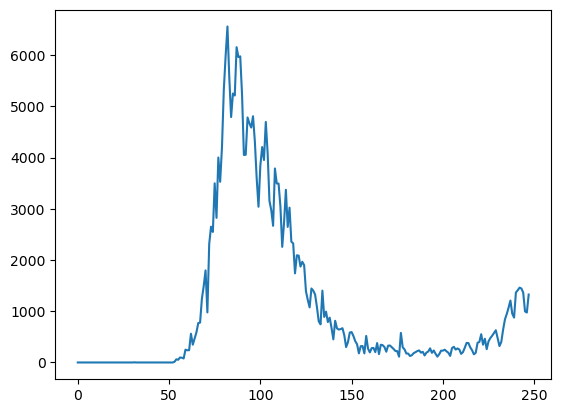
\includegraphics{Data visualization_files/figure-pdf/cell-5-output-2.png}

}

\end{figure}

While this plot shows the overall trend, it's hard to tell where the
peak occurred, as there are no dates on the X-axis. We can use the date
column as the index for the data frame to address this issue since it is
a time series dataset

\begin{Shaded}
\begin{Highlighting}[]
\NormalTok{covid\_df.set\_index(}\StringTok{\textquotesingle{}date\textquotesingle{}}\NormalTok{, inplace}\OperatorTok{=}\VariableTok{True}\NormalTok{)}
\end{Highlighting}
\end{Shaded}

\begin{Shaded}
\begin{Highlighting}[]
\NormalTok{covid\_df.new\_cases.plot(rot}\OperatorTok{=}\DecValTok{45}\NormalTok{)}
\end{Highlighting}
\end{Shaded}

\begin{verbatim}
<Axes: xlabel='date'>
\end{verbatim}

\begin{figure}[H]

{\centering 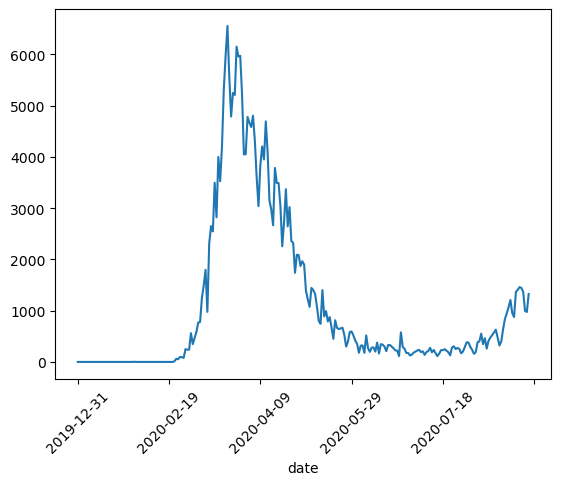
\includegraphics{Data visualization_files/figure-pdf/cell-7-output-2.png}

}

\end{figure}

With the date set as the index, we can observe that the peak occurred
around March 2020. Next, let's plot both new cases and new deaths
together to compare their trends over the same time period.

\begin{Shaded}
\begin{Highlighting}[]
\NormalTok{covid\_df[[}\StringTok{\textquotesingle{}new\_deaths\textquotesingle{}}\NormalTok{, }\StringTok{\textquotesingle{}new\_cases\textquotesingle{}}\NormalTok{]].plot()}
\end{Highlighting}
\end{Shaded}

\begin{verbatim}
<Axes: xlabel='date'>
\end{verbatim}

\begin{figure}[H]

{\centering 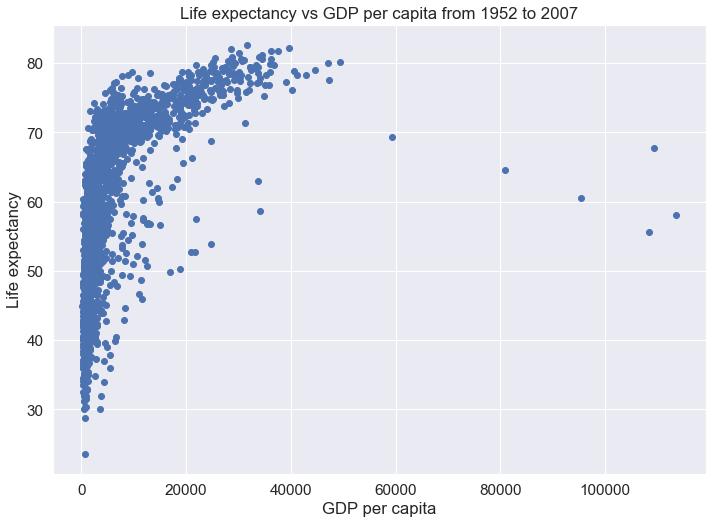
\includegraphics{Data visualization_files/figure-pdf/cell-8-output-2.png}

}

\end{figure}

By default, pandas generates line plots when using the
\href{https://pandas.pydata.org/docs/reference/api/pandas.DataFrame.plot.html}{\texttt{.plot}}
method. However, there are several parameters you can adjust to enhance
the appearance of the line plot.

\begin{Shaded}
\begin{Highlighting}[]
\NormalTok{covid\_df[[}\StringTok{\textquotesingle{}new\_deaths\textquotesingle{}}\NormalTok{, }\StringTok{\textquotesingle{}new\_cases\textquotesingle{}}\NormalTok{]].plot(figsize}\OperatorTok{=}\NormalTok{(}\DecValTok{12}\NormalTok{, }\DecValTok{6}\NormalTok{), linewidth}\OperatorTok{=}\DecValTok{2}\NormalTok{, marker}\OperatorTok{=}\StringTok{\textquotesingle{}o\textquotesingle{}}\NormalTok{)}
\end{Highlighting}
\end{Shaded}

\begin{verbatim}
<Axes: xlabel='date'>
\end{verbatim}

\begin{figure}[H]

{\centering 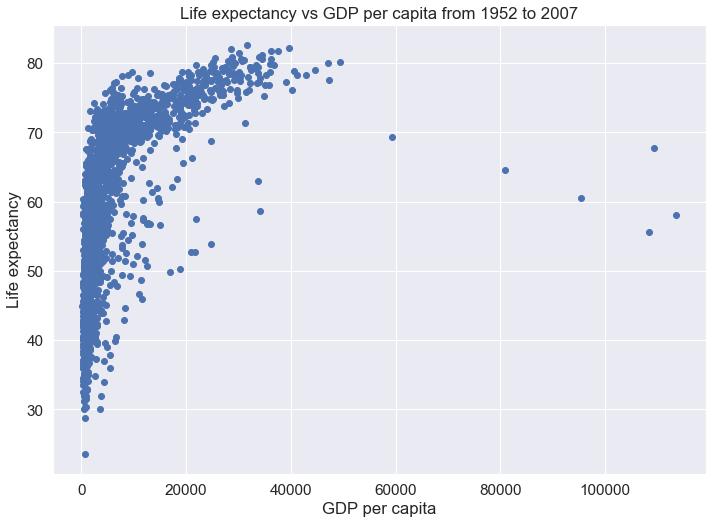
\includegraphics{Data visualization_files/figure-pdf/cell-9-output-2.png}

}

\end{figure}

You can create other types of visualizations by setting the kind
parameter in the plot function. The kind parameter accepts eleven
different string values, which specify the type of plot:

\begin{itemize}
\tightlist
\item
  ``area'' is for area plots.
\item
  ``bar'' is for vertical bar charts.
\item
  ``barh'' is for horizontal bar charts.
\item
  ``box'' is for box plots.
\item
  ``hexbin'' is for hexbin plots.
\item
  ``hist'' is for histograms.
\item
  ``kde'' is for kernel density estimate charts.
\item
  ``density'' is an alias for ``kde''.
\item
  ``line'' is for line graphs.
\item
  ``pie'' is for pie charts.
\item
  ``scatter'' is for scatter plots.
\end{itemize}

Let's next create a scatter plot to visualize the relationship between
new cases and new deaths, and explore whether there's a correlation
between them.

\begin{Shaded}
\begin{Highlighting}[]
\NormalTok{covid\_df.plot(kind}\OperatorTok{=}\StringTok{\textquotesingle{}scatter\textquotesingle{}}\NormalTok{, x}\OperatorTok{=}\StringTok{\textquotesingle{}new\_cases\textquotesingle{}}\NormalTok{, y}\OperatorTok{=}\StringTok{\textquotesingle{}new\_deaths\textquotesingle{}}\NormalTok{, color}\OperatorTok{=}\StringTok{\textquotesingle{}r\textquotesingle{}}\NormalTok{, alpha}\OperatorTok{=}\FloatTok{0.5}\NormalTok{)}\OperatorTok{;}
\end{Highlighting}
\end{Shaded}

\begin{figure}[H]

{\centering 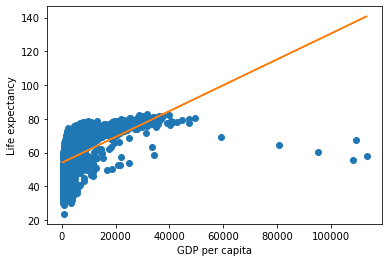
\includegraphics{Data visualization_files/figure-pdf/cell-10-output-1.png}

}

\end{figure}

Next, let's examine the distribution of new deaths using a histogram.

\begin{Shaded}
\begin{Highlighting}[]
\NormalTok{covid\_df.new\_deaths.plot(kind}\OperatorTok{=}\StringTok{\textquotesingle{}hist\textquotesingle{}}\NormalTok{, color}\OperatorTok{=}\StringTok{\textquotesingle{}r\textquotesingle{}}\NormalTok{, alpha}\OperatorTok{=}\FloatTok{0.5}\NormalTok{, bins}\OperatorTok{=}\DecValTok{50}\NormalTok{)}\OperatorTok{;}
\end{Highlighting}
\end{Shaded}

\begin{figure}[H]

{\centering \includegraphics{Data visualization_files/figure-pdf/cell-11-output-1.png}

}

\end{figure}

\begin{Shaded}
\begin{Highlighting}[]
\NormalTok{covid\_df.new\_cases.plot(kind}\OperatorTok{=}\StringTok{\textquotesingle{}box\textquotesingle{}}\NormalTok{)}\OperatorTok{;}
\end{Highlighting}
\end{Shaded}

\begin{figure}[H]

{\centering 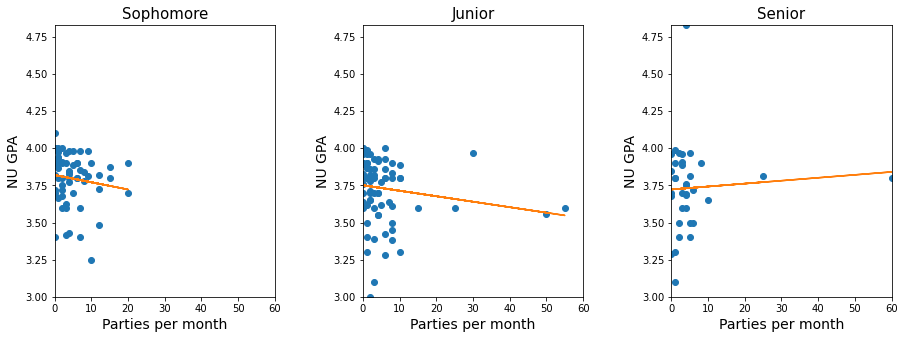
\includegraphics{Data visualization_files/figure-pdf/cell-12-output-1.png}

}

\end{figure}

For more plot types and detailed information, refer to the official
pandas documentation:

\begin{itemize}
\tightlist
\item
  \href{https://pandas.pydata.org/docs/reference/api/pandas.Series.plot.html}{Series.plot}
\item
  \href{https://pandas.pydata.org/docs/reference/api/pandas.DataFrame.plot.html}{DataFrame.plot}
\end{itemize}

\hypertarget{limitation-of-using-pandas-for-plotting}{%
\subsubsection{Limitation of using pandas for
plotting}\label{limitation-of-using-pandas-for-plotting}}

While pandas provides a straightforward way to create plots, there are
some limitations to be aware of:

\begin{itemize}
\item
  Customization: Pandas offers basic customization options, but it may
  not provide the level of detail or flexibility that you can achieve
  with matplotlib directly. For complex visualizations, you might need
  to switch to matplotlib for more control.
\item
  Plot Types: The range of plot types available in pandas is limited
  compared to what you can create with matplotlib or seaborn. For
  instance, advanced plots like violin plots or 3D plots require
  switching to other libraries.
\item
  Aesthetic Choices: The default aesthetics in pandas may not be as
  visually appealing as those created using seaborn or other specialized
  visualization libraries. For polished presentations, additional
  customization might be necessary.
\end{itemize}

\hypertarget{data-plotting-with-matplotlib-pyplot-interface}{%
\subsection{\texorpdfstring{Data Plotting with Matplotlib
\texttt{Pyplot}
Interface}{Data Plotting with Matplotlib Pyplot Interface}}\label{data-plotting-with-matplotlib-pyplot-interface}}

Pandas data visualization is built on top of matplotlib. When you use
the \texttt{.plot()} method in pandas, it internally calls matplotlib
functions to create the plots.

\href{https://matplotlib.org/}{Matplotlib} is:

\begin{itemize}
\tightlist
\item
  a low-level graph plotting library in python that strives to emulate
  MATLAB,
\item
  can be used in Python scripts, Python and IPython shells, Jupyter
  notebooks and web application servers.
\item
  is mostly written in python, a few segments are written in C,
  Objective-C and Javascript for Platform compatibility.
\end{itemize}

\hypertarget{matplotlib-pyplot}{%
\subsubsection{Matplotlib pyplot}\label{matplotlib-pyplot}}

\begin{itemize}
\tightlist
\item
  Matplotlib is the whole package; pyplot is a module in matplotlib
\item
  Most of the Matplotlib utilities lies under the pyplot module, and are
  usually imported under the plt alias:
\end{itemize}

\begin{Shaded}
\begin{Highlighting}[]
\ImportTok{import}\NormalTok{ matplotlib.pyplot }\ImportTok{as}\NormalTok{ plt}
\end{Highlighting}
\end{Shaded}

\hypertarget{data-source}{%
\subsubsection{Data Source}\label{data-source}}

\begin{itemize}
\tightlist
\item
  Python lists, NumPy arrays as well as a pandas series
\item
  However, all the sequences are internally converted to numpy arrays.
\end{itemize}

Let's create a python list to illustrate basic plotting with Matplotlib
pyplot

\begin{Shaded}
\begin{Highlighting}[]
\NormalTok{yield\_apples }\OperatorTok{=}\NormalTok{ [}\FloatTok{0.895}\NormalTok{, }\FloatTok{0.91}\NormalTok{, }\FloatTok{0.919}\NormalTok{, }\FloatTok{0.926}\NormalTok{, }\FloatTok{0.929}\NormalTok{, }\FloatTok{0.931}\NormalTok{]}
\end{Highlighting}
\end{Shaded}

\hypertarget{basic-plotting}{%
\subsubsection{Basic Plotting}\label{basic-plotting}}

\hypertarget{plotting-the-overall-trend}{%
\paragraph{Plotting the overall
trend}\label{plotting-the-overall-trend}}

\begin{Shaded}
\begin{Highlighting}[]
\NormalTok{plt.plot(yield\_apples)}
\end{Highlighting}
\end{Shaded}

\begin{figure}[H]

{\centering 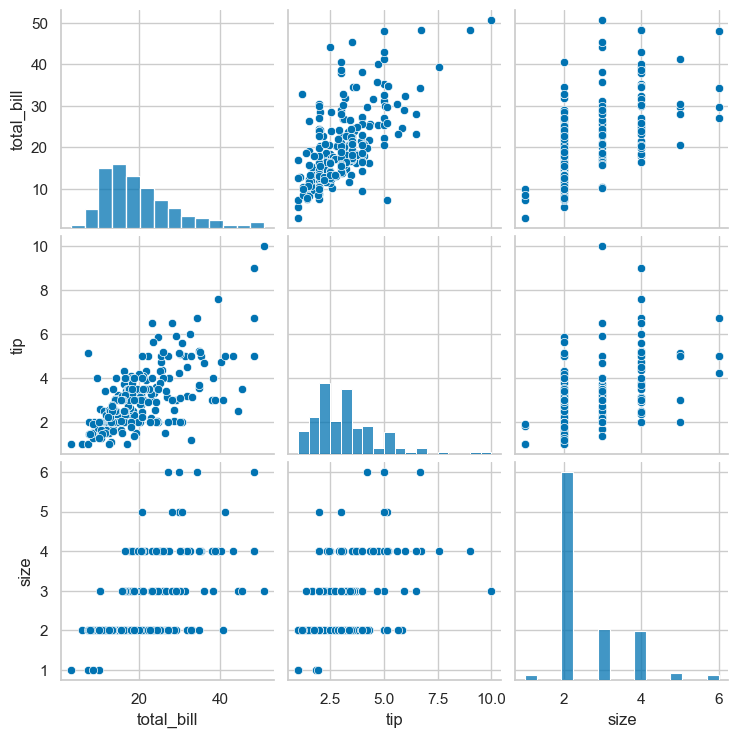
\includegraphics{Data visualization_files/figure-pdf/cell-15-output-1.png}

}

\end{figure}

Calling the \texttt{plt.plot} function draws the line chart as expected.
It also returns a list of plots drawn
\texttt{{[}\textless{}matplotlib.lines.Line2D\ at\ 0x2194b571df0\textgreater{}{]}},
shown within the output. We can include a semicolon (\texttt{;}) at the
end of the last statement in the cell to avoiding showing the output and
display just the graph.

\begin{Shaded}
\begin{Highlighting}[]
\NormalTok{plt.plot(yield\_apples)}\OperatorTok{;}
\end{Highlighting}
\end{Shaded}

\begin{figure}[H]

{\centering 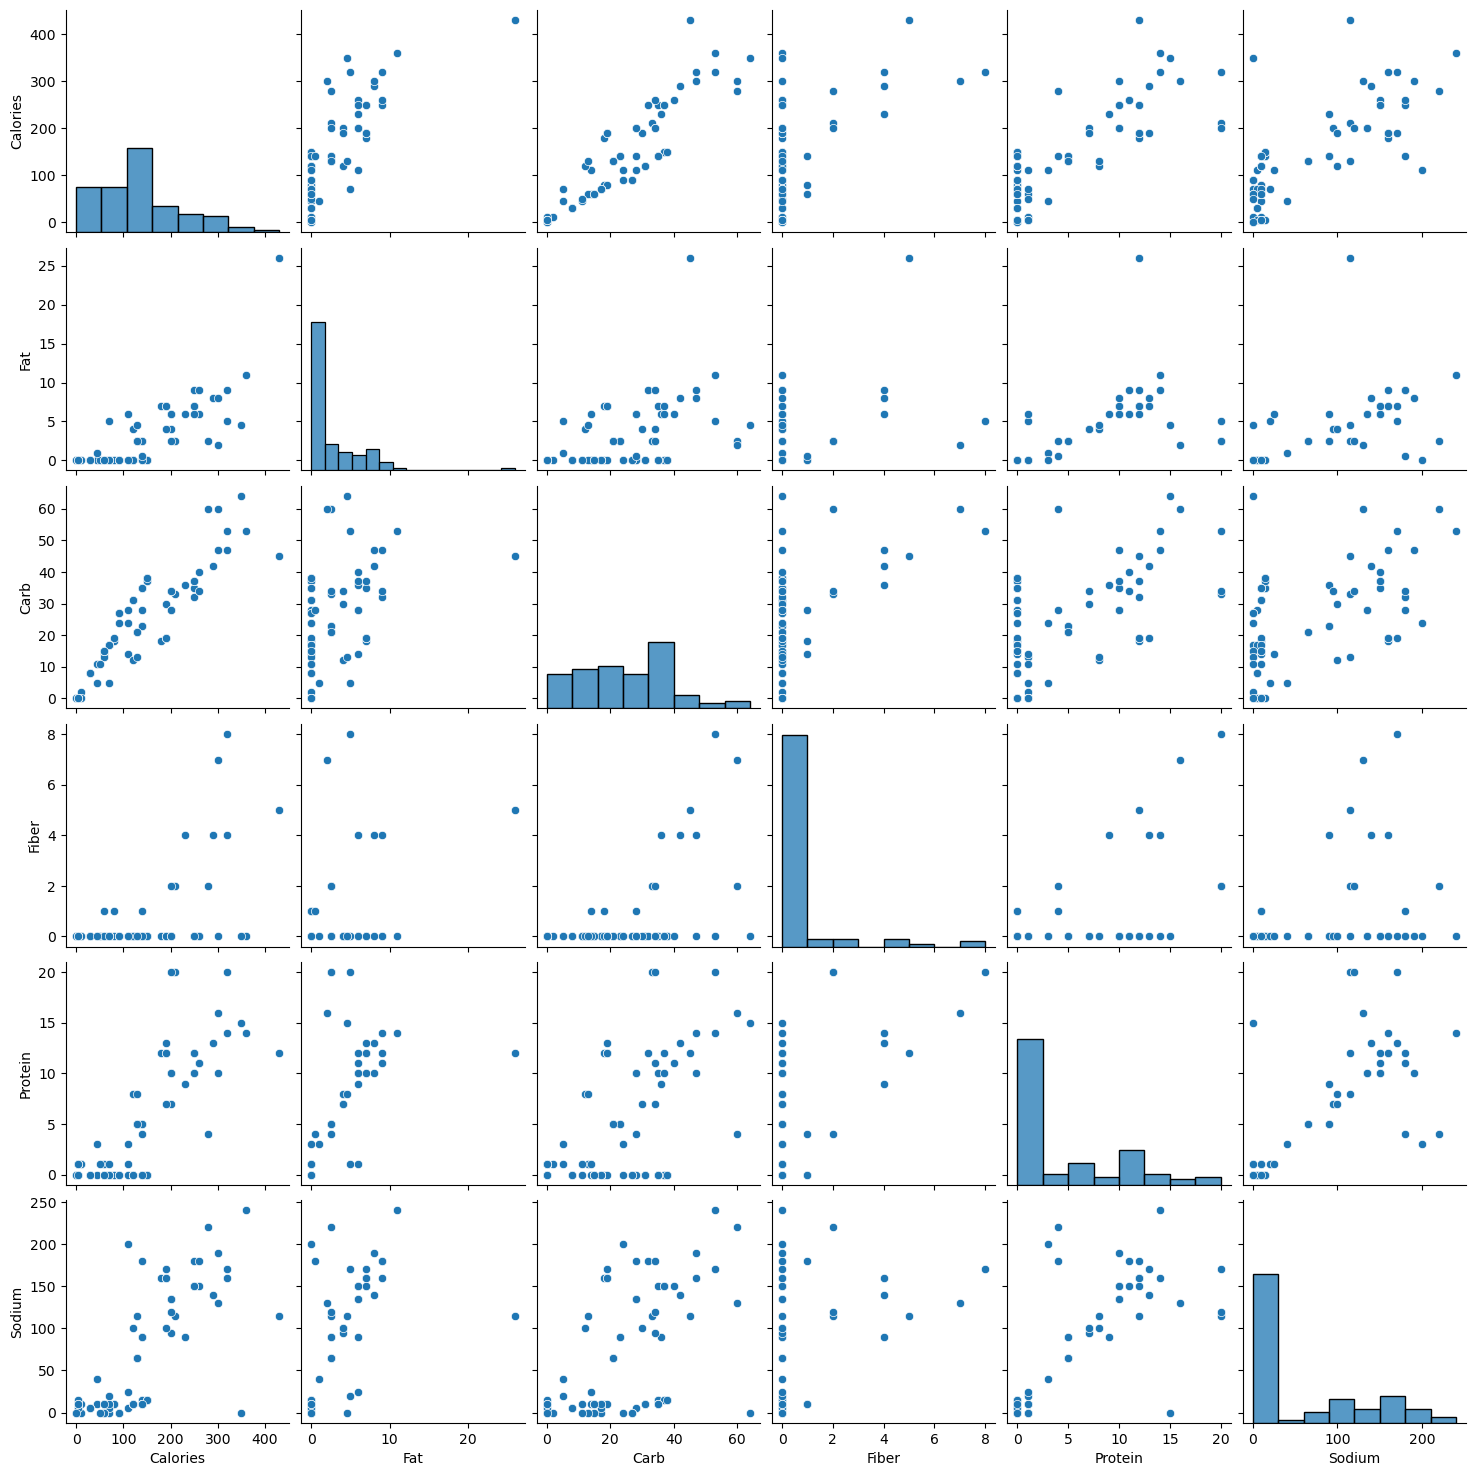
\includegraphics{Data visualization_files/figure-pdf/cell-16-output-1.png}

}

\end{figure}

\hypertarget{customizing-the-x-axis}{%
\paragraph{Customizing the X-axis}\label{customizing-the-x-axis}}

The X-axis of the plot currently shows list element indexes 0 to 5. The
plot would be more informative if we could display the year for which
we're plotting the data. We can do this by two arguments
\texttt{plt.plot}.

\begin{Shaded}
\begin{Highlighting}[]
\NormalTok{years }\OperatorTok{=}\NormalTok{ [}\DecValTok{2010}\NormalTok{, }\DecValTok{2011}\NormalTok{, }\DecValTok{2012}\NormalTok{, }\DecValTok{2013}\NormalTok{, }\DecValTok{2014}\NormalTok{, }\DecValTok{2015}\NormalTok{]}
\NormalTok{yield\_apples }\OperatorTok{=}\NormalTok{ [}\FloatTok{0.895}\NormalTok{, }\FloatTok{0.91}\NormalTok{, }\FloatTok{0.919}\NormalTok{, }\FloatTok{0.926}\NormalTok{, }\FloatTok{0.929}\NormalTok{, }\FloatTok{0.931}\NormalTok{]}
\end{Highlighting}
\end{Shaded}

\begin{Shaded}
\begin{Highlighting}[]
\NormalTok{plt.plot(years, yield\_apples)}\OperatorTok{;}
\end{Highlighting}
\end{Shaded}

\begin{figure}[H]

{\centering 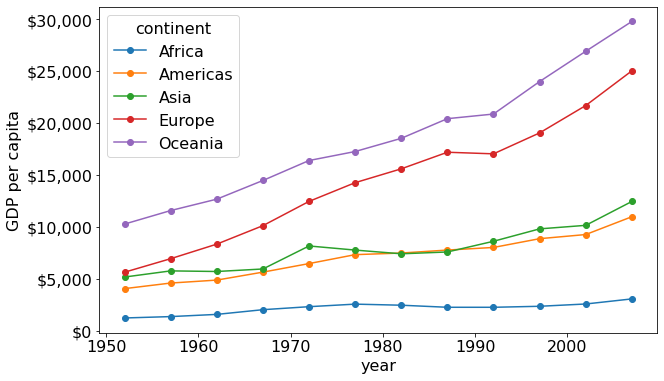
\includegraphics{Data visualization_files/figure-pdf/cell-18-output-1.png}

}

\end{figure}

\hypertarget{ploting-multiple-lines}{%
\paragraph{Ploting multiple lines}\label{ploting-multiple-lines}}

You can invoke the \texttt{plt.plot} function once for each line to plot
multiple lines in the same graph. Let's compare the yields of apples
vs.~oranges.

\begin{Shaded}
\begin{Highlighting}[]
\NormalTok{years }\OperatorTok{=} \BuiltInTok{range}\NormalTok{(}\DecValTok{2000}\NormalTok{, }\DecValTok{2012}\NormalTok{)}
\NormalTok{apples }\OperatorTok{=}\NormalTok{ [}\FloatTok{0.895}\NormalTok{, }\FloatTok{0.91}\NormalTok{, }\FloatTok{0.919}\NormalTok{, }\FloatTok{0.926}\NormalTok{, }\FloatTok{0.929}\NormalTok{, }\FloatTok{0.931}\NormalTok{, }\FloatTok{0.934}\NormalTok{, }\FloatTok{0.936}\NormalTok{, }\FloatTok{0.937}\NormalTok{, }\FloatTok{0.9375}\NormalTok{, }\FloatTok{0.9372}\NormalTok{, }\FloatTok{0.939}\NormalTok{]}
\NormalTok{oranges }\OperatorTok{=}\NormalTok{ [}\FloatTok{0.962}\NormalTok{, }\FloatTok{0.941}\NormalTok{, }\FloatTok{0.930}\NormalTok{, }\FloatTok{0.923}\NormalTok{, }\FloatTok{0.918}\NormalTok{, }\FloatTok{0.908}\NormalTok{, }\FloatTok{0.907}\NormalTok{, }\FloatTok{0.904}\NormalTok{, }\FloatTok{0.901}\NormalTok{, }\FloatTok{0.898}\NormalTok{, }\FloatTok{0.9}\NormalTok{, }\FloatTok{0.896}\NormalTok{, ]}
\end{Highlighting}
\end{Shaded}

\begin{Shaded}
\begin{Highlighting}[]
\NormalTok{plt.plot(years, apples)}
\NormalTok{plt.plot(years, oranges)}\OperatorTok{;}
\end{Highlighting}
\end{Shaded}

\begin{figure}[H]

{\centering 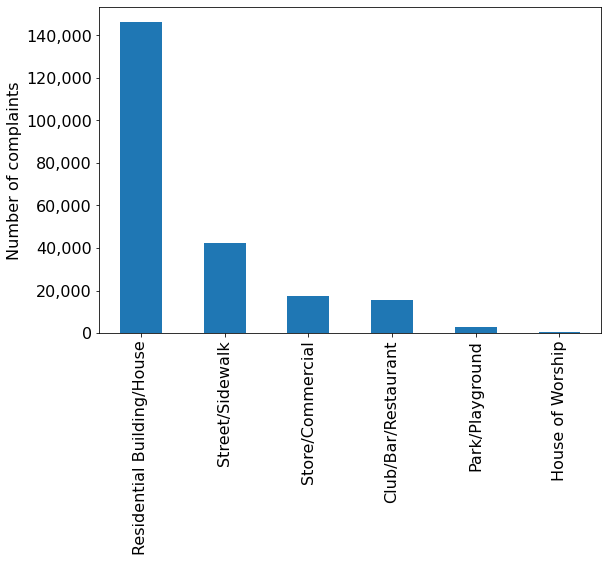
\includegraphics{Data visualization_files/figure-pdf/cell-20-output-1.png}

}

\end{figure}

When plt.plot command is called without any formatting parameters,
pyplot uses the following defaults:

\begin{itemize}
\tightlist
\item
  Figure size: 6.4 X 4.8 inches
\item
  Plot style: solid line
\item
  Linewidth: 1.5
\item
  Color: Blue (code `b', hex code: `\#1f77b4')
\end{itemize}

You can also edit default styles directly by modifying the
\texttt{matplotlib.rcParams} dictionary. Learn more:
https://matplotlib.org/3.2.1/tutorials/introductory/customizing.html\#matplotlib-rcparams
.

You can customize default plot styles by directly modifying the
\texttt{matplotlib.rcParams} dictionary. For more details, visit the
official Matplotlib guide on
\href{https://matplotlib.org/3.2.1/tutorials/introductory/customizing.html\#matplotlib-rcparams}{customizing
with rcParams}.

\begin{Shaded}
\begin{Highlighting}[]
\ImportTok{import}\NormalTok{ matplotlib}
\NormalTok{matplotlib.rcParams[}\StringTok{\textquotesingle{}font.size\textquotesingle{}}\NormalTok{] }\OperatorTok{=} \DecValTok{14}
\NormalTok{matplotlib.rcParams[}\StringTok{\textquotesingle{}figure.figsize\textquotesingle{}}\NormalTok{] }\OperatorTok{=}\NormalTok{ (}\DecValTok{7}\NormalTok{, }\DecValTok{4}\NormalTok{)}
\NormalTok{matplotlib.rcParams[}\StringTok{\textquotesingle{}figure.facecolor\textquotesingle{}}\NormalTok{] }\OperatorTok{=} \StringTok{\textquotesingle{}\#00000000\textquotesingle{}}
\end{Highlighting}
\end{Shaded}

\textbf{Conceptual model}: Plotting in Matplotlib involves multiple
levels of control, from setting the figure size to customizing
individual text elements. To offer complete control over the plotting
process, Matplotlib provides an object-oriented interface in a
hierarchical structure. This approach allows users to create and manage
\texttt{Figure} and \texttt{Axes} objects, which serve as the foundation
for all plotting actions. In the next chapter, you will explore how to
use this object-oriented interface to gain more precise control over
your plots.

\hypertarget{enhancing-the-plot}{%
\subsubsection{Enhancing the plot}\label{enhancing-the-plot}}

Matplotlib provides a wide range of customizable components within a
figure, allowing for fine-tuned control over every aspect of the plot.
These components include elements like axes, labels, ticks, legends, and
the overall layout. Each can be tailored to enhance the clarity,
aesthetics, and effectiveness of the visual representation, making the
plot more engaging and easier to interpret.

\begin{figure}

{\centering 

\begin{verbatim}
<IPython.core.display.Image object>
\end{verbatim}

}

\caption{\label{fig-anatomy}Matplotlib anatomy of a figure}

\end{figure}

\hypertarget{adding-axis-lables}{%
\paragraph{Adding Axis Lables}\label{adding-axis-lables}}

We can add labels to the axes to show what each axis represents using
the \texttt{plt.xlabel} and \texttt{plt.ylabel} methods.

\begin{Shaded}
\begin{Highlighting}[]
\NormalTok{plt.plot(years, apples)}
\NormalTok{plt.plot(years, oranges)}
\NormalTok{plt.xlabel(}\StringTok{\textquotesingle{}Year\textquotesingle{}}\NormalTok{)}
\NormalTok{plt.ylabel(}\StringTok{\textquotesingle{}Yield (tons per hectare)\textquotesingle{}}\NormalTok{)}\OperatorTok{;}
\end{Highlighting}
\end{Shaded}

\begin{figure}[H]

{\centering 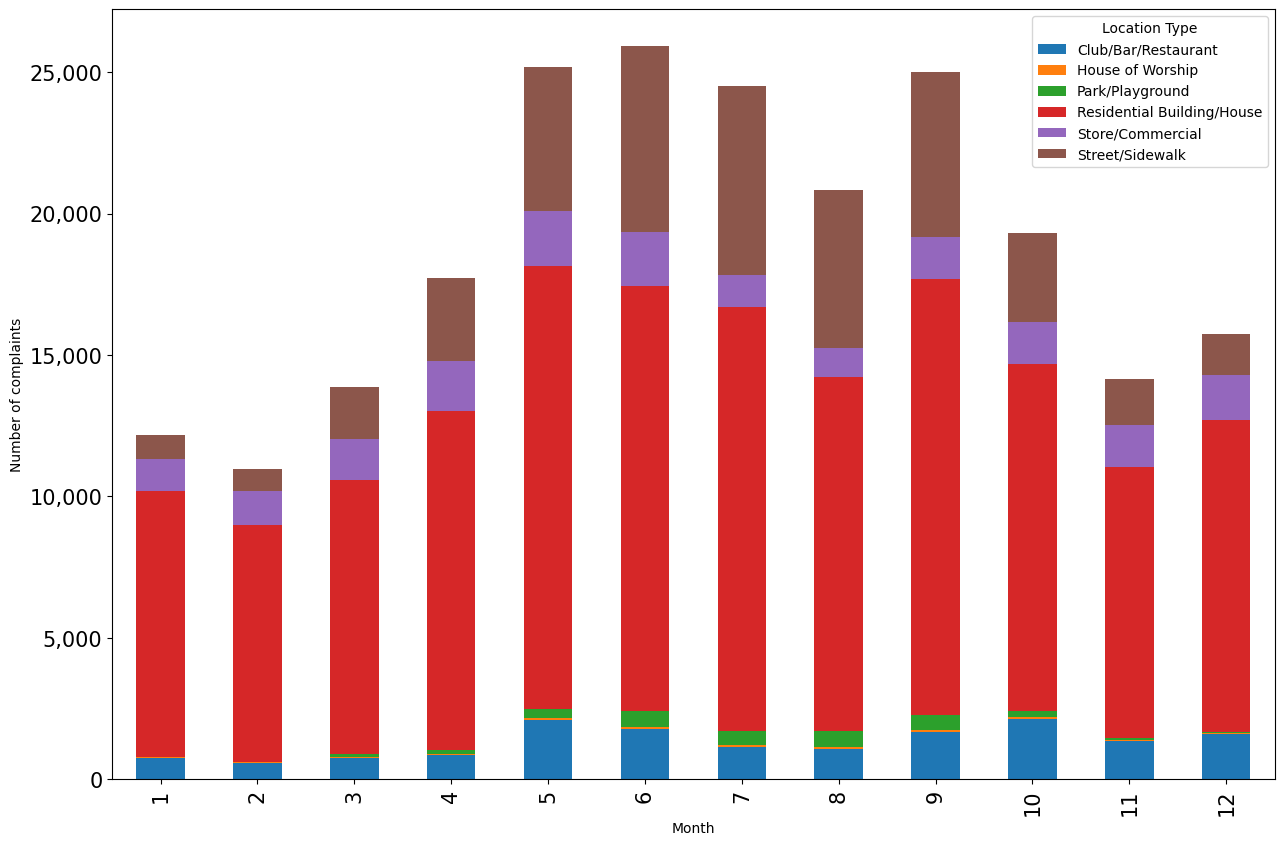
\includegraphics{Data visualization_files/figure-pdf/cell-23-output-1.png}

}

\end{figure}

\hypertarget{adding-chart-title-and-legend}{%
\paragraph{Adding Chart Title and
Legend}\label{adding-chart-title-and-legend}}

To differentiate between multiple lines, we can include a legend within
the graph using the \texttt{plt.legend} function. We can also set a
title for the chart using the \texttt{plt.title} function.

\begin{Shaded}
\begin{Highlighting}[]
\NormalTok{plt.plot(years, apples)}
\NormalTok{plt.plot(years, oranges)}

\NormalTok{plt.xlabel(}\StringTok{\textquotesingle{}Year\textquotesingle{}}\NormalTok{)}
\NormalTok{plt.ylabel(}\StringTok{\textquotesingle{}Yield (tons per hectare)\textquotesingle{}}\NormalTok{)}

\NormalTok{plt.title(}\StringTok{"Crop Yields in Kanto"}\NormalTok{)}
\NormalTok{plt.legend([}\StringTok{\textquotesingle{}Apples\textquotesingle{}}\NormalTok{, }\StringTok{\textquotesingle{}Oranges\textquotesingle{}}\NormalTok{])}\OperatorTok{;}
\end{Highlighting}
\end{Shaded}

\begin{figure}[H]

{\centering 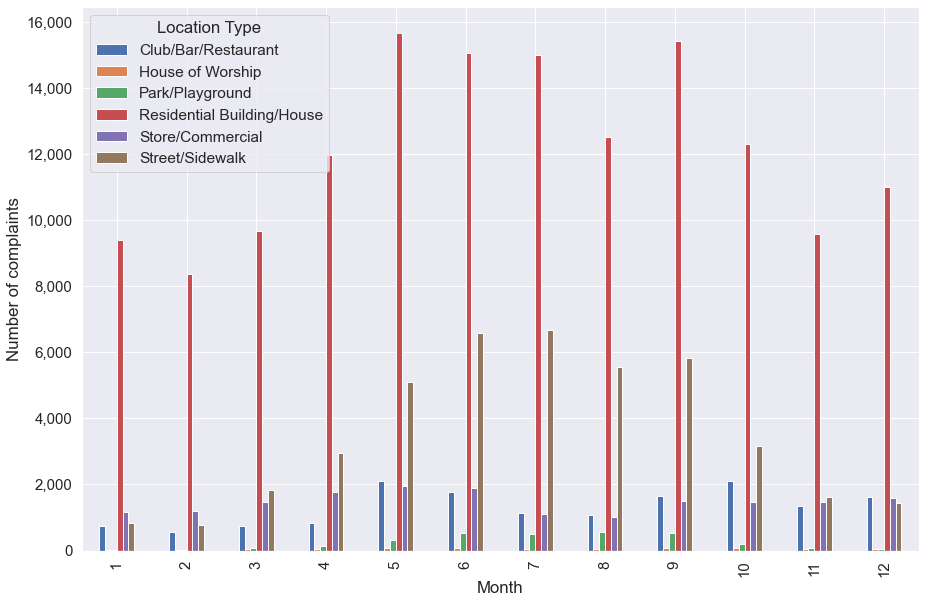
\includegraphics{Data visualization_files/figure-pdf/cell-24-output-1.png}

}

\end{figure}

\hypertarget{adding-line-markers}{%
\paragraph{Adding Line Markers}\label{adding-line-markers}}

We can also show markers for the data points on each line using the
\texttt{marker} argument of \texttt{plt.plot}. Matplotlib provides many
different markers, like a circle, cross, square, diamond, etc. You can
find the full list of marker types
\href{https://matplotlib.org/3.1.1/api/markers_api.html}{here}.

\begin{Shaded}
\begin{Highlighting}[]
\NormalTok{plt.plot(years, apples, marker}\OperatorTok{=}\StringTok{\textquotesingle{}o\textquotesingle{}}\NormalTok{)}
\NormalTok{plt.plot(years, oranges, marker}\OperatorTok{=}\StringTok{\textquotesingle{}x\textquotesingle{}}\NormalTok{)}

\NormalTok{plt.xlabel(}\StringTok{\textquotesingle{}Year\textquotesingle{}}\NormalTok{)}
\NormalTok{plt.ylabel(}\StringTok{\textquotesingle{}Yield (tons per hectare)\textquotesingle{}}\NormalTok{)}

\NormalTok{plt.title(}\StringTok{"Crop Yields in Kanto"}\NormalTok{)}
\NormalTok{plt.legend([}\StringTok{\textquotesingle{}Apples\textquotesingle{}}\NormalTok{, }\StringTok{\textquotesingle{}Oranges\textquotesingle{}}\NormalTok{])}\OperatorTok{;}
\end{Highlighting}
\end{Shaded}

\begin{figure}[H]

{\centering 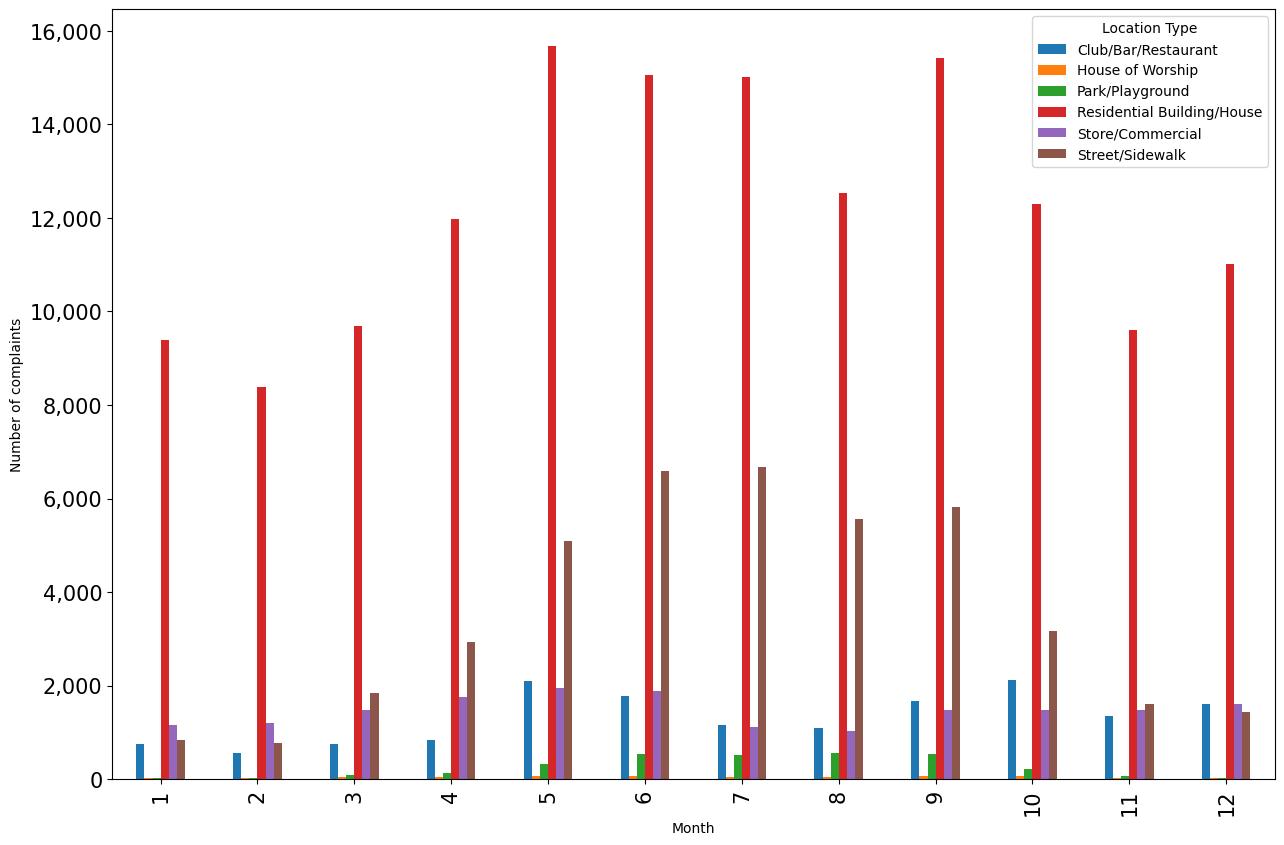
\includegraphics{Data visualization_files/figure-pdf/cell-25-output-1.png}

}

\end{figure}

\hypertarget{styling-lines-and-markers}{%
\paragraph{Styling Lines and Markers}\label{styling-lines-and-markers}}

The \texttt{plt.plot} function supports many arguments for styling lines
and markers:

\begin{itemize}
\tightlist
\item
  \texttt{color} or \texttt{c}: Set the color of the line
  (\href{https://matplotlib.org/3.1.0/gallery/color/named_colors.html}{supported
  colors})
\item
  \texttt{linestyle} or \texttt{ls}: Choose between a solid or dashed
  line
\item
  \texttt{linewidth} or \texttt{lw}: Set the width of a line
\item
  \texttt{markersize} or \texttt{ms}: Set the size of markers
\item
  \texttt{markeredgecolor} or \texttt{mec}: Set the edge color for
  markers
\item
  \texttt{markeredgewidth} or \texttt{mew}: Set the edge width for
  markers
\item
  \texttt{markerfacecolor} or \texttt{mfc}: Set the fill color for
  markers
\item
  \texttt{alpha}: Opacity of the plot
\end{itemize}

Check out the documentation for \texttt{plt.plot} to learn more:
\url{https://matplotlib.org/api/_as_gen/matplotlib.pyplot.plot.html\#matplotlib.pyplot.plot}
.

\begin{Shaded}
\begin{Highlighting}[]
\NormalTok{plt.plot(years, apples, marker}\OperatorTok{=}\StringTok{\textquotesingle{}s\textquotesingle{}}\NormalTok{, c}\OperatorTok{=}\StringTok{\textquotesingle{}b\textquotesingle{}}\NormalTok{, ls}\OperatorTok{=}\StringTok{\textquotesingle{}{-}\textquotesingle{}}\NormalTok{, lw}\OperatorTok{=}\DecValTok{2}\NormalTok{, ms}\OperatorTok{=}\DecValTok{8}\NormalTok{, mew}\OperatorTok{=}\DecValTok{2}\NormalTok{, mec}\OperatorTok{=}\StringTok{\textquotesingle{}navy\textquotesingle{}}\NormalTok{)}
\NormalTok{plt.plot(years, oranges, marker}\OperatorTok{=}\StringTok{\textquotesingle{}o\textquotesingle{}}\NormalTok{, c}\OperatorTok{=}\StringTok{\textquotesingle{}r\textquotesingle{}}\NormalTok{, ls}\OperatorTok{=}\StringTok{\textquotesingle{}{-}{-}\textquotesingle{}}\NormalTok{, lw}\OperatorTok{=}\DecValTok{3}\NormalTok{, ms}\OperatorTok{=}\DecValTok{10}\NormalTok{, alpha}\OperatorTok{=}\FloatTok{.5}\NormalTok{)}

\NormalTok{plt.xlabel(}\StringTok{\textquotesingle{}Year\textquotesingle{}}\NormalTok{)}
\NormalTok{plt.ylabel(}\StringTok{\textquotesingle{}Yield (tons per hectare)\textquotesingle{}}\NormalTok{)}

\NormalTok{plt.title(}\StringTok{"Crop Yields in Kanto"}\NormalTok{)}
\NormalTok{plt.legend([}\StringTok{\textquotesingle{}Apples\textquotesingle{}}\NormalTok{, }\StringTok{\textquotesingle{}Oranges\textquotesingle{}}\NormalTok{])}\OperatorTok{;}
\end{Highlighting}
\end{Shaded}

\begin{figure}[H]

{\centering 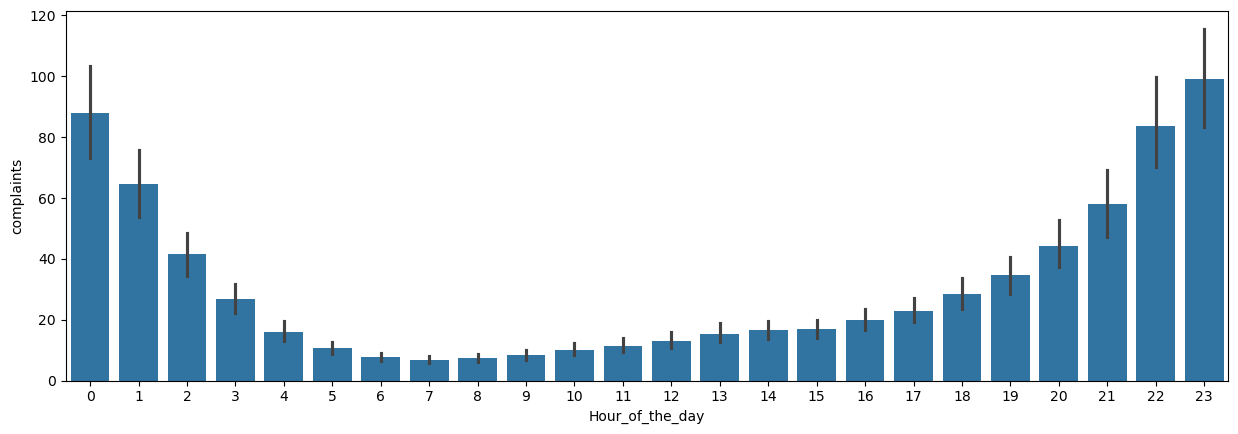
\includegraphics{Data visualization_files/figure-pdf/cell-26-output-1.png}

}

\end{figure}

The \texttt{fmt} argument provides a shorthand for specifying the marker
shape, line style, and line color. It can be provided as the third
argument to \texttt{plt.plot}.

\begin{verbatim}
fmt = '[marker][line][color]'
\end{verbatim}

\begin{Shaded}
\begin{Highlighting}[]
\NormalTok{plt.plot(years, apples, }\StringTok{\textquotesingle{}s{-}b\textquotesingle{}}\NormalTok{)}
\NormalTok{plt.plot(years, oranges, }\StringTok{\textquotesingle{}o{-}{-}r\textquotesingle{}}\NormalTok{)}

\NormalTok{plt.xlabel(}\StringTok{\textquotesingle{}Year\textquotesingle{}}\NormalTok{)}
\NormalTok{plt.ylabel(}\StringTok{\textquotesingle{}Yield (tons per hectare)\textquotesingle{}}\NormalTok{)}

\NormalTok{plt.title(}\StringTok{"Crop Yields in Kanto"}\NormalTok{)}
\NormalTok{plt.legend([}\StringTok{\textquotesingle{}Apples\textquotesingle{}}\NormalTok{, }\StringTok{\textquotesingle{}Oranges\textquotesingle{}}\NormalTok{])}\OperatorTok{;}
\end{Highlighting}
\end{Shaded}

\begin{figure}[H]

{\centering 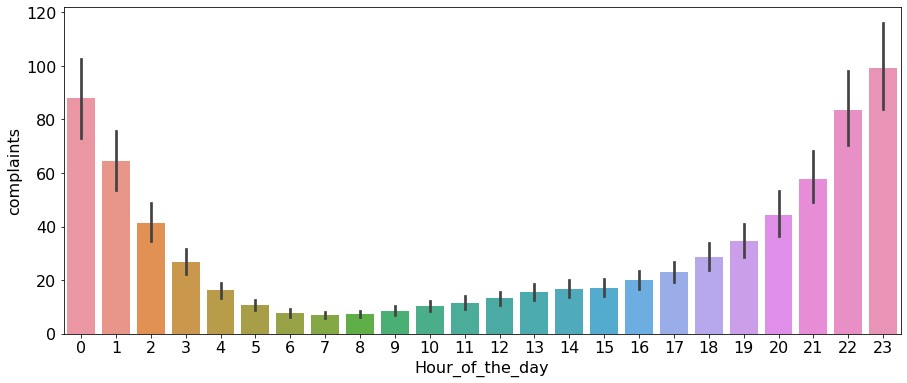
\includegraphics{Data visualization_files/figure-pdf/cell-27-output-1.png}

}

\end{figure}

If you don't specify a line style in \texttt{fmt}, only markers are
drawn.

\begin{Shaded}
\begin{Highlighting}[]
\NormalTok{plt.plot(years, apples, }\StringTok{\textquotesingle{}sb\textquotesingle{}}\NormalTok{)}
\NormalTok{plt.plot(years, oranges, }\StringTok{\textquotesingle{}or\textquotesingle{}}\NormalTok{)}
\NormalTok{plt.title(}\StringTok{"Yield (tons per hectare)"}\NormalTok{)}\OperatorTok{;}
\end{Highlighting}
\end{Shaded}

\begin{figure}[H]

{\centering 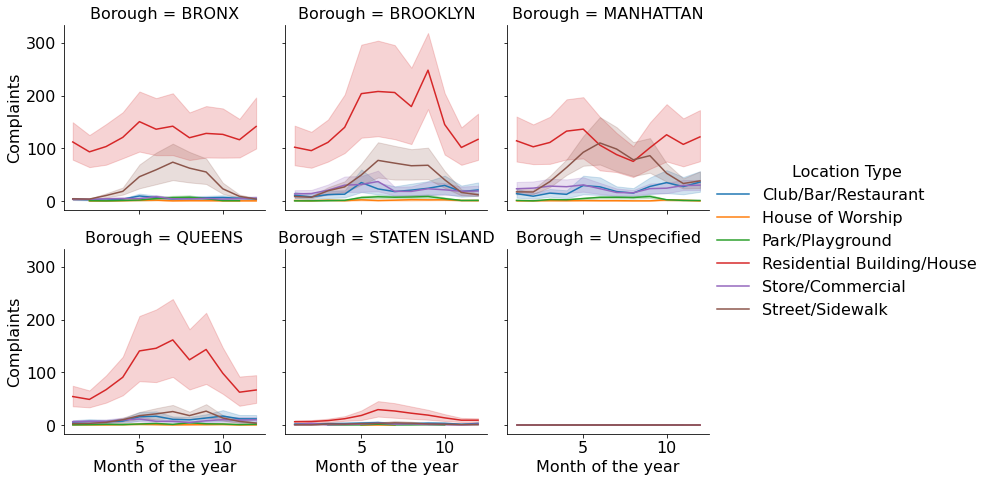
\includegraphics{Data visualization_files/figure-pdf/cell-28-output-1.png}

}

\end{figure}

\hypertarget{changing-the-figure-size}{%
\paragraph{Changing the Figure Size}\label{changing-the-figure-size}}

You can use the \texttt{plt.figure} function to change the size of the
figure.

\begin{Shaded}
\begin{Highlighting}[]
\NormalTok{plt.figure(figsize}\OperatorTok{=}\NormalTok{(}\DecValTok{6}\NormalTok{, }\DecValTok{4}\NormalTok{))}

\NormalTok{plt.plot(years, oranges, }\StringTok{\textquotesingle{}or\textquotesingle{}}\NormalTok{)}
\NormalTok{plt.title(}\StringTok{"Yield of Oranges (tons per hectare)"}\NormalTok{)}\OperatorTok{;}
\end{Highlighting}
\end{Shaded}

\begin{figure}[H]

{\centering 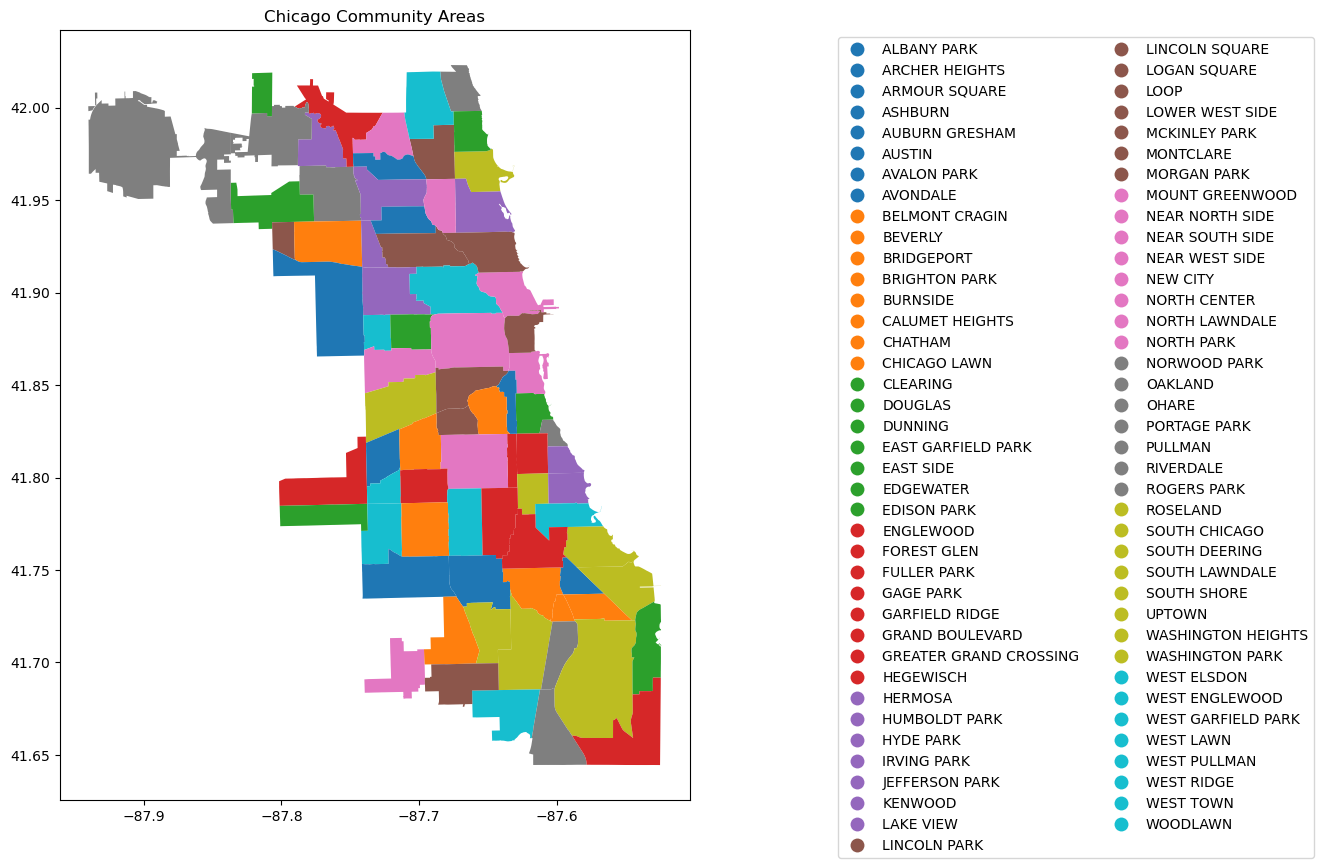
\includegraphics{Data visualization_files/figure-pdf/cell-29-output-1.png}

}

\end{figure}

\hypertarget{plotting-other-types-of-plots-with-matplotlib-pyplot}{%
\subsubsection{\texorpdfstring{Plotting other types of plots with
matplotlib
\texttt{pyplot}}{Plotting other types of plots with matplotlib pyplot}}\label{plotting-other-types-of-plots-with-matplotlib-pyplot}}

Let's read the \emph{fifa\_data.csv} as our data source

\begin{Shaded}
\begin{Highlighting}[]
\NormalTok{fifa }\OperatorTok{=}\NormalTok{ pd.read\_csv(}\StringTok{\textquotesingle{}./Datasets/fifa\_data.csv\textquotesingle{}}\NormalTok{)}
\NormalTok{fifa.head(}\DecValTok{5}\NormalTok{)}
\end{Highlighting}
\end{Shaded}

\begin{longtable}[]{@{}llllllllllllllllllllll@{}}
\toprule\noalign{}
& Unnamed: 0 & ID & Name & Age & Photo & Nationality & Flag & Overall &
Potential & Club & ... & Composure & Marking & StandingTackle &
SlidingTackle & GKDiving & GKHandling & GKKicking & GKPositioning &
GKReflexes & Release Clause \\
\midrule\noalign{}
\endhead
\bottomrule\noalign{}
\endlastfoot
0 & 0 & 158023 & L. Messi & 31 &
https://cdn.sofifa.org/players/4/19/158023.png & Argentina &
https://cdn.sofifa.org/flags/52.png & 94 & 94 & FC Barcelona & ... &
96.0 & 33.0 & 28.0 & 26.0 & 6.0 & 11.0 & 15.0 & 14.0 & 8.0 & €226.5M \\
1 & 1 & 20801 & Cristiano Ronaldo & 33 &
https://cdn.sofifa.org/players/4/19/20801.png & Portugal &
https://cdn.sofifa.org/flags/38.png & 94 & 94 & Juventus & ... & 95.0 &
28.0 & 31.0 & 23.0 & 7.0 & 11.0 & 15.0 & 14.0 & 11.0 & €127.1M \\
2 & 2 & 190871 & Neymar Jr & 26 &
https://cdn.sofifa.org/players/4/19/190871.png & Brazil &
https://cdn.sofifa.org/flags/54.png & 92 & 93 & Paris Saint-Germain &
... & 94.0 & 27.0 & 24.0 & 33.0 & 9.0 & 9.0 & 15.0 & 15.0 & 11.0 &
€228.1M \\
3 & 3 & 193080 & De Gea & 27 &
https://cdn.sofifa.org/players/4/19/193080.png & Spain &
https://cdn.sofifa.org/flags/45.png & 91 & 93 & Manchester United & ...
& 68.0 & 15.0 & 21.0 & 13.0 & 90.0 & 85.0 & 87.0 & 88.0 & 94.0 &
€138.6M \\
4 & 4 & 192985 & K. De Bruyne & 27 &
https://cdn.sofifa.org/players/4/19/192985.png & Belgium &
https://cdn.sofifa.org/flags/7.png & 91 & 92 & Manchester City & ... &
88.0 & 68.0 & 58.0 & 51.0 & 15.0 & 13.0 & 5.0 & 10.0 & 13.0 & €196.4M \\
\end{longtable}

\hypertarget{histgram}{%
\paragraph{Histgram}\label{histgram}}

\begin{Shaded}
\begin{Highlighting}[]
\NormalTok{plt.figure(figsize}\OperatorTok{=}\NormalTok{(}\DecValTok{8}\NormalTok{,}\DecValTok{5}\NormalTok{))}

\NormalTok{plt.hist(fifa.Overall, color}\OperatorTok{=}\StringTok{\textquotesingle{}\#abcdef\textquotesingle{}}\NormalTok{)}

\NormalTok{plt.ylabel(}\StringTok{\textquotesingle{}Number of Players\textquotesingle{}}\NormalTok{)}
\NormalTok{plt.xlabel(}\StringTok{\textquotesingle{}Skill Level\textquotesingle{}}\NormalTok{)}
\NormalTok{plt.title(}\StringTok{\textquotesingle{}Distribution of Player Skills in FIFA 2018\textquotesingle{}}\NormalTok{)}
\end{Highlighting}
\end{Shaded}

\begin{verbatim}
Text(0.5, 1.0, 'Distribution of Player Skills in FIFA 2018')
\end{verbatim}

\begin{figure}[H]

{\centering 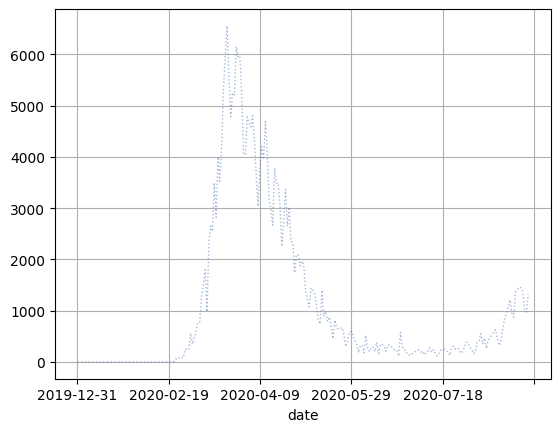
\includegraphics{Data visualization_files/figure-pdf/cell-31-output-2.png}

}

\end{figure}

\hypertarget{bar-chart}{%
\paragraph{Bar chart}\label{bar-chart}}

\begin{Shaded}
\begin{Highlighting}[]
\CommentTok{\# plotting bar chart for the best players}
\NormalTok{plt.figure(figsize}\OperatorTok{=}\NormalTok{(}\DecValTok{8}\NormalTok{,}\DecValTok{5}\NormalTok{))}

\NormalTok{foot\_preference }\OperatorTok{=}\NormalTok{ fifa[}\StringTok{\textquotesingle{}Preferred Foot\textquotesingle{}}\NormalTok{].value\_counts()}

\NormalTok{plt.bar([}\StringTok{\textquotesingle{}Left\textquotesingle{}}\NormalTok{, }\StringTok{\textquotesingle{}Right\textquotesingle{}}\NormalTok{], [foot\_preference.iloc[}\DecValTok{1}\NormalTok{], foot\_preference.iloc[}\DecValTok{0}\NormalTok{]], color}\OperatorTok{=}\StringTok{\textquotesingle{}\#abcdef\textquotesingle{}}\NormalTok{)}

\NormalTok{plt.ylabel(}\StringTok{\textquotesingle{}Number of Players\textquotesingle{}}\NormalTok{)}
\NormalTok{plt.title(}\StringTok{\textquotesingle{}Foot Preference of FIFA Players\textquotesingle{}}\NormalTok{)}\OperatorTok{;}
\end{Highlighting}
\end{Shaded}

\begin{figure}[H]

{\centering 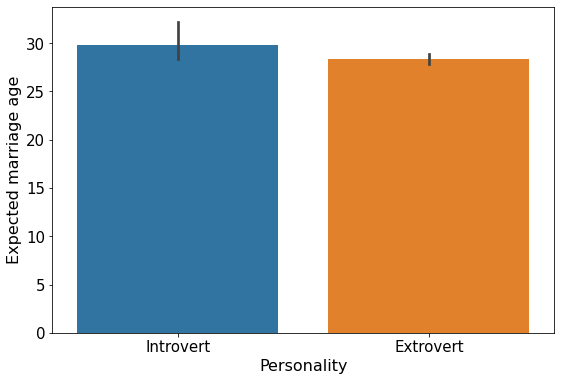
\includegraphics{Data visualization_files/figure-pdf/cell-32-output-1.png}

}

\end{figure}

\hypertarget{pie-chart}{%
\paragraph{Pie chart}\label{pie-chart}}

\begin{Shaded}
\begin{Highlighting}[]
\NormalTok{left }\OperatorTok{=}\NormalTok{ fifa.loc[fifa[}\StringTok{\textquotesingle{}Preferred Foot\textquotesingle{}}\NormalTok{] }\OperatorTok{==} \StringTok{\textquotesingle{}Left\textquotesingle{}}\NormalTok{].count().iloc[}\DecValTok{0}\NormalTok{]}
\NormalTok{right }\OperatorTok{=}\NormalTok{ fifa.loc[fifa[}\StringTok{\textquotesingle{}Preferred Foot\textquotesingle{}}\NormalTok{] }\OperatorTok{==} \StringTok{\textquotesingle{}Right\textquotesingle{}}\NormalTok{].count().iloc[}\DecValTok{0}\NormalTok{]}

\NormalTok{plt.figure(figsize}\OperatorTok{=}\NormalTok{(}\DecValTok{8}\NormalTok{,}\DecValTok{5}\NormalTok{))}

\NormalTok{labels }\OperatorTok{=}\NormalTok{ [}\StringTok{\textquotesingle{}Left\textquotesingle{}}\NormalTok{, }\StringTok{\textquotesingle{}Right\textquotesingle{}}\NormalTok{]}
\NormalTok{colors }\OperatorTok{=}\NormalTok{ [}\StringTok{\textquotesingle{}\#abcdef\textquotesingle{}}\NormalTok{, }\StringTok{\textquotesingle{}\#aabbcc\textquotesingle{}}\NormalTok{]}

\NormalTok{plt.pie([left, right], labels }\OperatorTok{=}\NormalTok{ labels, colors}\OperatorTok{=}\NormalTok{colors, autopct}\OperatorTok{=}\StringTok{\textquotesingle{}}\SpecialCharTok{\%.2f}\StringTok{ }\SpecialCharTok{\%\%}\StringTok{\textquotesingle{}}\NormalTok{)}

\NormalTok{plt.title(}\StringTok{\textquotesingle{}Foot Preference of FIFA Players\textquotesingle{}}\NormalTok{)}\OperatorTok{;}
\end{Highlighting}
\end{Shaded}

\begin{figure}[H]

{\centering 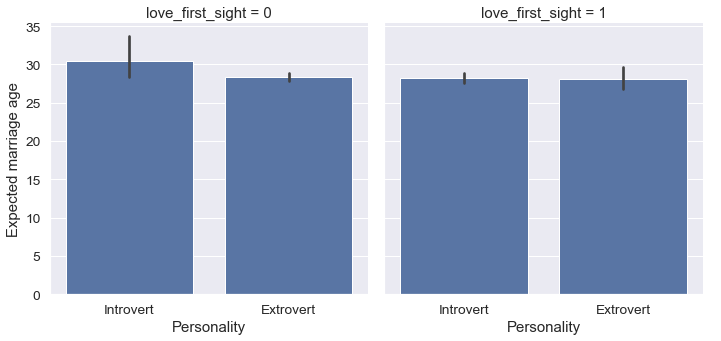
\includegraphics{Data visualization_files/figure-pdf/cell-33-output-1.png}

}

\end{figure}

Another Pie Chart on wight of players

\begin{Shaded}
\begin{Highlighting}[]
\NormalTok{plt.figure(figsize}\OperatorTok{=}\NormalTok{(}\DecValTok{8}\NormalTok{,}\DecValTok{5}\NormalTok{), dpi}\OperatorTok{=}\DecValTok{100}\NormalTok{)}

\NormalTok{plt.style.use(}\StringTok{\textquotesingle{}ggplot\textquotesingle{}}\NormalTok{)}

\NormalTok{fifa.Weight }\OperatorTok{=}\NormalTok{ [}\BuiltInTok{int}\NormalTok{(x.strip(}\StringTok{\textquotesingle{}lbs\textquotesingle{}}\NormalTok{)) }\ControlFlowTok{if} \BuiltInTok{type}\NormalTok{(x)}\OperatorTok{==}\BuiltInTok{str} \ControlFlowTok{else}\NormalTok{ x }\ControlFlowTok{for}\NormalTok{ x }\KeywordTok{in}\NormalTok{ fifa.Weight]}

\NormalTok{light }\OperatorTok{=}\NormalTok{ fifa.loc[fifa.Weight }\OperatorTok{\textless{}} \DecValTok{125}\NormalTok{].count().iloc[}\DecValTok{0}\NormalTok{]}
\NormalTok{light\_medium }\OperatorTok{=}\NormalTok{ fifa[(fifa.Weight }\OperatorTok{\textgreater{}=} \DecValTok{125}\NormalTok{) }\OperatorTok{\&}\NormalTok{ (fifa.Weight }\OperatorTok{\textless{}} \DecValTok{150}\NormalTok{)].count().iloc[}\DecValTok{0}\NormalTok{]}
\NormalTok{medium }\OperatorTok{=}\NormalTok{ fifa[(fifa.Weight }\OperatorTok{\textgreater{}=} \DecValTok{150}\NormalTok{) }\OperatorTok{\&}\NormalTok{ (fifa.Weight }\OperatorTok{\textless{}} \DecValTok{175}\NormalTok{)].count().iloc[}\DecValTok{0}\NormalTok{]}
\NormalTok{medium\_heavy }\OperatorTok{=}\NormalTok{ fifa[(fifa.Weight }\OperatorTok{\textgreater{}=} \DecValTok{175}\NormalTok{) }\OperatorTok{\&}\NormalTok{ (fifa.Weight }\OperatorTok{\textless{}} \DecValTok{200}\NormalTok{)].count().iloc[}\DecValTok{0}\NormalTok{]}
\NormalTok{heavy }\OperatorTok{=}\NormalTok{ fifa[fifa.Weight }\OperatorTok{\textgreater{}=} \DecValTok{200}\NormalTok{].count().iloc[}\DecValTok{0}\NormalTok{]}

\NormalTok{weights }\OperatorTok{=}\NormalTok{ [light,light\_medium, medium, medium\_heavy, heavy]}
\NormalTok{label }\OperatorTok{=}\NormalTok{ [}\StringTok{\textquotesingle{}under 125\textquotesingle{}}\NormalTok{, }\StringTok{\textquotesingle{}125{-}150\textquotesingle{}}\NormalTok{, }\StringTok{\textquotesingle{}150{-}175\textquotesingle{}}\NormalTok{, }\StringTok{\textquotesingle{}175{-}200\textquotesingle{}}\NormalTok{, }\StringTok{\textquotesingle{}over 200\textquotesingle{}}\NormalTok{]}
\NormalTok{explode }\OperatorTok{=}\NormalTok{ (}\FloatTok{.4}\NormalTok{,}\FloatTok{.2}\NormalTok{,}\DecValTok{0}\NormalTok{,}\DecValTok{0}\NormalTok{,}\FloatTok{.4}\NormalTok{)}

\NormalTok{plt.title(}\StringTok{\textquotesingle{}Weight of Professional Soccer Players (lbs)\textquotesingle{}}\NormalTok{)}

\NormalTok{plt.pie(weights, labels}\OperatorTok{=}\NormalTok{label, explode}\OperatorTok{=}\NormalTok{explode, pctdistance}\OperatorTok{=}\FloatTok{0.8}\NormalTok{,autopct}\OperatorTok{=}\StringTok{\textquotesingle{}}\SpecialCharTok{\%.2f}\StringTok{ }\SpecialCharTok{\%\%}\StringTok{\textquotesingle{}}\NormalTok{)}\OperatorTok{;}
\end{Highlighting}
\end{Shaded}

\begin{figure}[H]

{\centering 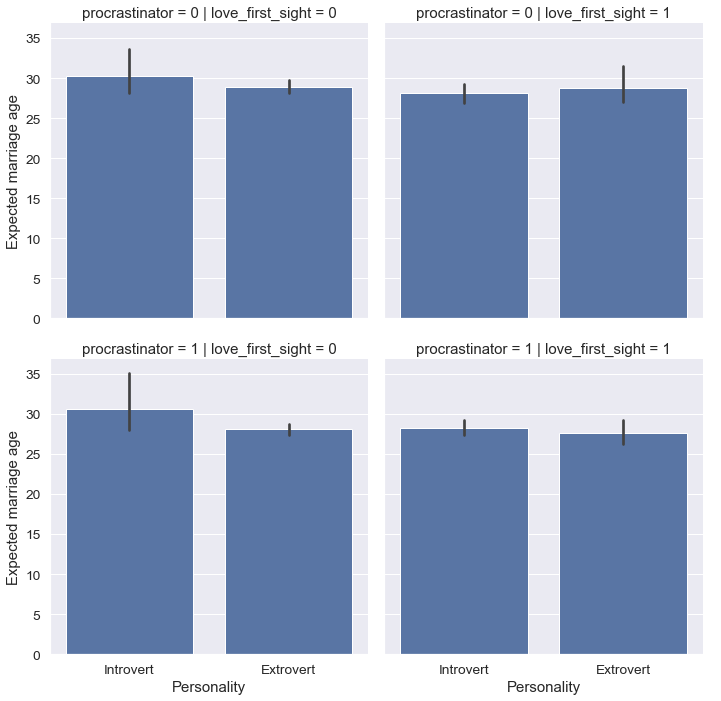
\includegraphics{Data visualization_files/figure-pdf/cell-34-output-1.png}

}

\end{figure}

\hypertarget{box-and-whiskers-chart}{%
\paragraph{Box and Whiskers Chart}\label{box-and-whiskers-chart}}

\begin{Shaded}
\begin{Highlighting}[]
\NormalTok{plt.figure(figsize}\OperatorTok{=}\NormalTok{(}\DecValTok{5}\NormalTok{,}\DecValTok{8}\NormalTok{), dpi}\OperatorTok{=}\DecValTok{100}\NormalTok{)}

\NormalTok{plt.style.use(}\StringTok{\textquotesingle{}default\textquotesingle{}}\NormalTok{)}

\NormalTok{barcelona }\OperatorTok{=}\NormalTok{ fifa.loc[fifa.Club }\OperatorTok{==} \StringTok{"FC Barcelona"}\NormalTok{][}\StringTok{\textquotesingle{}Overall\textquotesingle{}}\NormalTok{]}
\NormalTok{madrid }\OperatorTok{=}\NormalTok{ fifa.loc[fifa.Club }\OperatorTok{==} \StringTok{"Real Madrid"}\NormalTok{][}\StringTok{\textquotesingle{}Overall\textquotesingle{}}\NormalTok{]}
\NormalTok{revs }\OperatorTok{=}\NormalTok{ fifa.loc[fifa.Club }\OperatorTok{==} \StringTok{"New England Revolution"}\NormalTok{][}\StringTok{\textquotesingle{}Overall\textquotesingle{}}\NormalTok{]}

\CommentTok{\#bp = plt.boxplot([barcelona, madrid, revs], labels=[\textquotesingle{}a\textquotesingle{},\textquotesingle{}b\textquotesingle{},\textquotesingle{}c\textquotesingle{}], boxprops=dict(facecolor=\textquotesingle{}red\textquotesingle{}))}
\NormalTok{bp }\OperatorTok{=}\NormalTok{ plt.boxplot([barcelona, madrid, revs], tick\_labels}\OperatorTok{=}\NormalTok{[}\StringTok{\textquotesingle{}FC Barcelona\textquotesingle{}}\NormalTok{,}\StringTok{\textquotesingle{}Real Madrid\textquotesingle{}}\NormalTok{,}\StringTok{\textquotesingle{}NE Revolution\textquotesingle{}}\NormalTok{], patch\_artist}\OperatorTok{=}\VariableTok{True}\NormalTok{, medianprops}\OperatorTok{=}\NormalTok{\{}\StringTok{\textquotesingle{}linewidth\textquotesingle{}}\NormalTok{: }\DecValTok{2}\NormalTok{\})}

\NormalTok{plt.title(}\StringTok{\textquotesingle{}Professional Soccer Team Comparison\textquotesingle{}}\NormalTok{)}
\NormalTok{plt.ylabel(}\StringTok{\textquotesingle{}FIFA Overall Rating\textquotesingle{}}\NormalTok{)}

\ControlFlowTok{for}\NormalTok{ box }\KeywordTok{in}\NormalTok{ bp[}\StringTok{\textquotesingle{}boxes\textquotesingle{}}\NormalTok{]:}
    \CommentTok{\# change outline color}
\NormalTok{    box.}\BuiltInTok{set}\NormalTok{(color}\OperatorTok{=}\StringTok{\textquotesingle{}\#4286f4\textquotesingle{}}\NormalTok{, linewidth}\OperatorTok{=}\DecValTok{2}\NormalTok{)}
    \CommentTok{\# change fill color}
\NormalTok{    box.}\BuiltInTok{set}\NormalTok{(facecolor }\OperatorTok{=} \StringTok{\textquotesingle{}\#e0e0e0\textquotesingle{}}\NormalTok{ )}
    \CommentTok{\# change hatch}
    \CommentTok{\#box.set(hatch = \textquotesingle{}/\textquotesingle{})}
\end{Highlighting}
\end{Shaded}

\begin{figure}[H]

{\centering 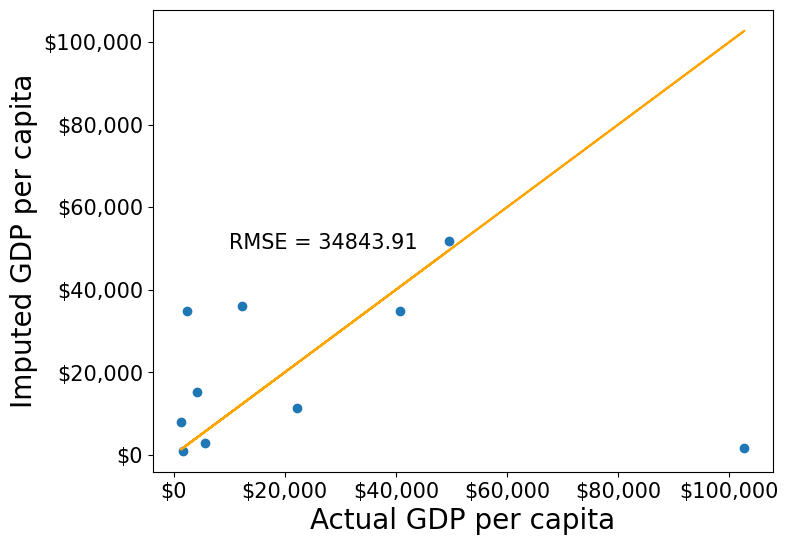
\includegraphics{Data visualization_files/figure-pdf/cell-35-output-1.png}

}

\end{figure}

You've already learned how to create plots using Matplotlib's
\texttt{Pyplot}. Next, you'll explore how to simplify and enhance your
visualizations by using its powerful wrappers: Pandas and Seaborn.

\hypertarget{limitations-of-using-matplotlib-for-plotting}{%
\subsubsection{Limitations of Using Matplotlib for
Plotting}\label{limitations-of-using-matplotlib-for-plotting}}

Matplotlib is a popular visualization library, but it has flaws.

\begin{itemize}
\tightlist
\item
  Defaults are not ideal (gridlines, background, etc need to be
  configured.)
\item
  Library is low-level (doing anything complicated takes quite a bit of
  codes)
\item
  Lack of integration with pandas data structures
\end{itemize}

To address these challenges, Seaborn act as higher-level interfaces to
Matplotlib, offering better defaults, simpler syntax, and seamless
integration with DataFrames.

\hypertarget{plotting-with-seaborn}{%
\subsection{Plotting with Seaborn}\label{plotting-with-seaborn}}

Seaborn is a powerful data visualization library built on top of
Matplotlib, designed to make statistical plots easier and more
attractive. It integrates seamlessly with Pandas, making it an excellent
tool for plotting data from DataFrames. Seaborn comes with better
default aesthetics and provides more specialized plots that are easy to
implement.

Some of the key advantages of using Seaborn include:

\begin{itemize}
\tightlist
\item
  \textbf{Simpler syntax}: Seaborn simplifies the process of creating
  complex plots with just a few lines of code.
\item
  \textbf{Beautiful default styles}: Seaborn's default plots are more
  polished and aesthetically pleasing compared to Matplotlib's defaults.
\item
  \textbf{Seamless Pandas integration}: You can directly pass Pandas
  DataFrames to Seaborn, and it understands column names for axis labels
  and plot elements.
\end{itemize}

\texttt{seaborn} comes with 17 built-in datasets. That means you don't
have to spend a whole lot of your time finding the right dataset and
cleaning it up to make Seaborn-ready; rather you will focus on the core
features of Seaborn visualization techniques to solve problems.

\begin{Shaded}
\begin{Highlighting}[]
\ImportTok{import}\NormalTok{ seaborn }\ImportTok{as}\NormalTok{ sns}
\CommentTok{\# get names of the builtin dataset}
\NormalTok{sns.get\_dataset\_names()}
\end{Highlighting}
\end{Shaded}

\begin{verbatim}
['anagrams',
 'anscombe',
 'attention',
 'brain_networks',
 'car_crashes',
 'diamonds',
 'dots',
 'dowjones',
 'exercise',
 'flights',
 'fmri',
 'geyser',
 'glue',
 'healthexp',
 'iris',
 'mpg',
 'penguins',
 'planets',
 'seaice',
 'taxis',
 'tips',
 'titanic']
\end{verbatim}

\hypertarget{customizing-plot-aesthetics}{%
\subsubsection{Customizing Plot
Aesthetics}\label{customizing-plot-aesthetics}}

Seaborn provides a convenient function called \texttt{sns.set\_style()}
that allows users to customize the visual appearance of their plots.
This function is particularly useful for enhancing the aesthetics of
visualizations, making them more appealing and easier to interpret.

\hypertarget{purpose-of-sns.set_style}{%
\paragraph{\texorpdfstring{Purpose of
\texttt{sns.set\_style()}}{Purpose of sns.set\_style()}}\label{purpose-of-sns.set_style}}

The primary purpose of \texttt{sns.set\_style()} is to set the visual
context and style for all plots created after the call. This allows for
a consistent and visually pleasing representation of data across
multiple visualizations.

\hypertarget{available-style-options}{%
\paragraph{Available Style Options}\label{available-style-options}}

Seaborn offers several built-in styles that can be set using
\texttt{sns.set\_style()}. The options include:

\begin{enumerate}
\def\labelenumi{\arabic{enumi}.}
\tightlist
\item
  \textbf{\texttt{darkgrid}}:

  \begin{itemize}
  \tightlist
  \item
    A dark background with a grid overlay.
  \item
    Ideal for visualizing data with many points or intricate details.
  \end{itemize}
\item
  \textbf{\texttt{whitegrid}}:

  \begin{itemize}
  \tightlist
  \item
    A white background with a grid overlay.
  \item
    Provides a clean and professional look, suitable for most types of
    visualizations.
  \end{itemize}
\item
  \textbf{\texttt{dark}}:

  \begin{itemize}
  \tightlist
  \item
    A dark background without gridlines.
  \item
    Useful for emphasizing data points without distractions from the
    grid.
  \end{itemize}
\item
  \textbf{\texttt{white}}:

  \begin{itemize}
  \tightlist
  \item
    A simple white background without gridlines.
  \item
    Offers a minimalist aesthetic, focusing solely on the data.
  \end{itemize}
\item
  \textbf{\texttt{ticks}}:

  \begin{itemize}
  \tightlist
  \item
    A white background with ticks on the axes.
  \item
    Combines the clarity of a white background with a bit of added
    detail for reference.
  \end{itemize}
\end{enumerate}

\hypertarget{how-to-use-sns.set_style}{%
\paragraph{\texorpdfstring{How to Use
\texttt{sns.set\_style()}}{How to Use sns.set\_style()}}\label{how-to-use-sns.set_style}}

To apply a specific style, simply call \texttt{sns.set\_style()} with
the desired style name before creating your plots. Here's an example:

\begin{Shaded}
\begin{Highlighting}[]
\NormalTok{sns.set\_style(}\StringTok{"whitegrid"}\NormalTok{)}
\end{Highlighting}
\end{Shaded}

Let's do a few common plots with Seaborn tips dataset

\begin{Shaded}
\begin{Highlighting}[]
\CommentTok{\# Load data into a Pandas dataframe}
\NormalTok{flowers\_df }\OperatorTok{=}\NormalTok{ sns.load\_dataset(}\StringTok{"iris"}\NormalTok{)}
\NormalTok{flowers\_df.head()}
\end{Highlighting}
\end{Shaded}

\begin{longtable}[]{@{}llllll@{}}
\toprule\noalign{}
& sepal\_length & sepal\_width & petal\_length & petal\_width &
species \\
\midrule\noalign{}
\endhead
\bottomrule\noalign{}
\endlastfoot
0 & 5.1 & 3.5 & 1.4 & 0.2 & setosa \\
1 & 4.9 & 3.0 & 1.4 & 0.2 & setosa \\
2 & 4.7 & 3.2 & 1.3 & 0.2 & setosa \\
3 & 4.6 & 3.1 & 1.5 & 0.2 & setosa \\
4 & 5.0 & 3.6 & 1.4 & 0.2 & setosa \\
\end{longtable}

\hypertarget{scatterplot}{%
\subsubsection{Scatterplot}\label{scatterplot}}

\begin{Shaded}
\begin{Highlighting}[]
\NormalTok{sns.scatterplot(x}\OperatorTok{=}\NormalTok{flowers\_df.sepal\_length, y}\OperatorTok{=}\NormalTok{flowers\_df.sepal\_width)}\OperatorTok{;}
\end{Highlighting}
\end{Shaded}

\begin{figure}[H]

{\centering 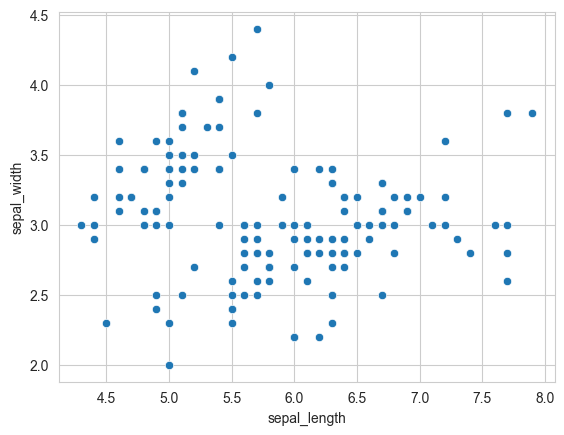
\includegraphics{Data visualization_files/figure-pdf/cell-39-output-1.png}

}

\end{figure}

\hypertarget{adding-hues-to-the-scatterplot}{%
\paragraph{Adding Hues to the
scatterplot}\label{adding-hues-to-the-scatterplot}}

Notice how the points in the above plot seem to form distinct clusters
with some outliers. We can color the dots using the flower species as a
\texttt{hue}. We can also make the points larger using the \texttt{s}
argument.

\begin{Shaded}
\begin{Highlighting}[]
\NormalTok{flowers\_df.species.unique()}
\end{Highlighting}
\end{Shaded}

\begin{verbatim}
array(['setosa', 'versicolor', 'virginica'], dtype=object)
\end{verbatim}

\begin{Shaded}
\begin{Highlighting}[]
\NormalTok{sns.scatterplot(x}\OperatorTok{=}\NormalTok{flowers\_df.sepal\_length, y}\OperatorTok{=}\NormalTok{flowers\_df.sepal\_width, hue}\OperatorTok{=}\NormalTok{flowers\_df.species, s}\OperatorTok{=}\DecValTok{100}\NormalTok{)}\OperatorTok{;}
\end{Highlighting}
\end{Shaded}

\begin{figure}[H]

{\centering 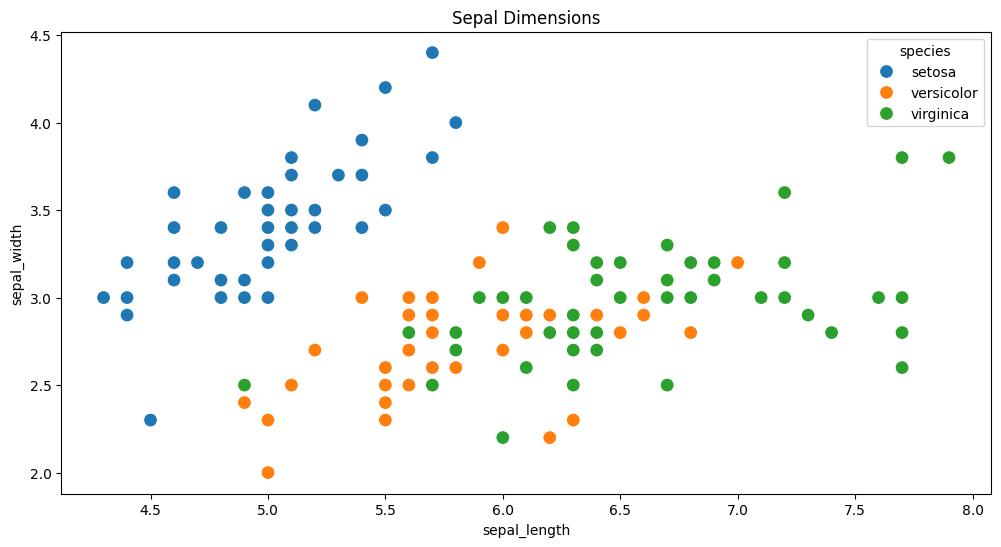
\includegraphics{Data visualization_files/figure-pdf/cell-41-output-1.png}

}

\end{figure}

Adding hues makes the plot more informative. We can immediately tell
that Setosa flowers have a smaller sepal length but higher sepal widths.
In contrast, the opposite is true for Virginica flowers.

\hypertarget{customizing-seaborn-figures}{%
\paragraph{Customizing Seaborn
Figures}\label{customizing-seaborn-figures}}

Since Seaborn uses Matplotlib's plotting functions internally, we can
use functions like \texttt{plt.figure} and \texttt{plt.title} to modify
the figure.

\begin{Shaded}
\begin{Highlighting}[]
\NormalTok{plt.figure(figsize}\OperatorTok{=}\NormalTok{(}\DecValTok{12}\NormalTok{, }\DecValTok{6}\NormalTok{))}
\NormalTok{plt.title(}\StringTok{\textquotesingle{}Sepal Dimensions\textquotesingle{}}\NormalTok{)}

\NormalTok{sns.scatterplot(x}\OperatorTok{=}\NormalTok{flowers\_df.sepal\_length, }
\NormalTok{                y}\OperatorTok{=}\NormalTok{flowers\_df.sepal\_width, }
\NormalTok{                hue}\OperatorTok{=}\NormalTok{flowers\_df.species,}
\NormalTok{                s}\OperatorTok{=}\DecValTok{100}\NormalTok{)}\OperatorTok{;}
\end{Highlighting}
\end{Shaded}

\begin{figure}[H]

{\centering 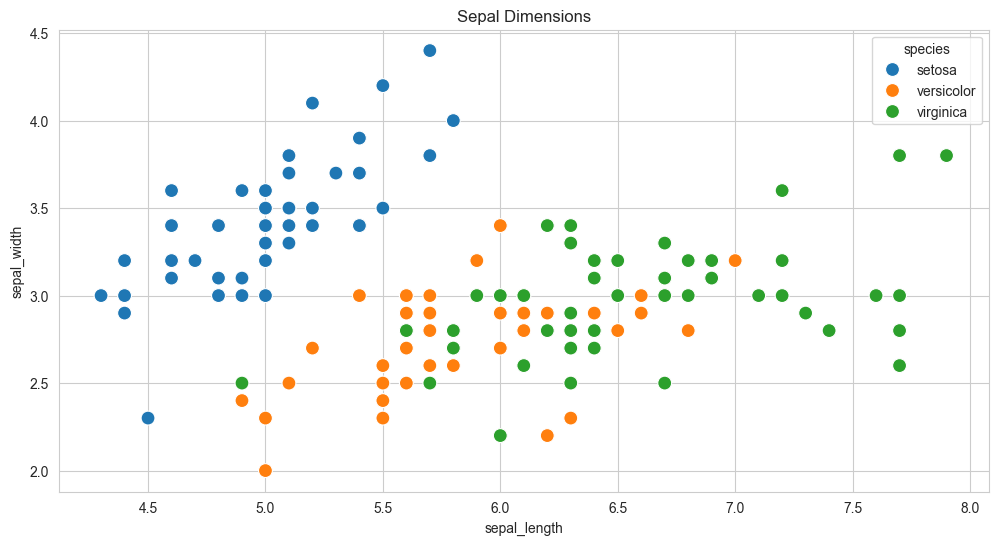
\includegraphics{Data visualization_files/figure-pdf/cell-42-output-1.png}

}

\end{figure}

\hypertarget{integration-with-pandas-data-frames}{%
\paragraph{Integration with Pandas Data
Frames}\label{integration-with-pandas-data-frames}}

Seaborn has in-built support for Pandas data frames. Instead of passing
each column as a series, you can provide column names and use the
\texttt{data} argument to specify a data frame.

\begin{Shaded}
\begin{Highlighting}[]
\NormalTok{plt.title(}\StringTok{\textquotesingle{}Sepal Dimensions\textquotesingle{}}\NormalTok{)}
\NormalTok{sns.scatterplot(x}\OperatorTok{=}\StringTok{\textquotesingle{}sepal\_length\textquotesingle{}}\NormalTok{, }
\NormalTok{                y}\OperatorTok{=}\StringTok{\textquotesingle{}sepal\_width\textquotesingle{}}\NormalTok{, }
\NormalTok{                hue}\OperatorTok{=}\StringTok{\textquotesingle{}species\textquotesingle{}}\NormalTok{,}
\NormalTok{                s}\OperatorTok{=}\DecValTok{100}\NormalTok{,}
\NormalTok{                data}\OperatorTok{=}\NormalTok{flowers\_df)}\OperatorTok{;}
\end{Highlighting}
\end{Shaded}

\begin{figure}[H]

{\centering 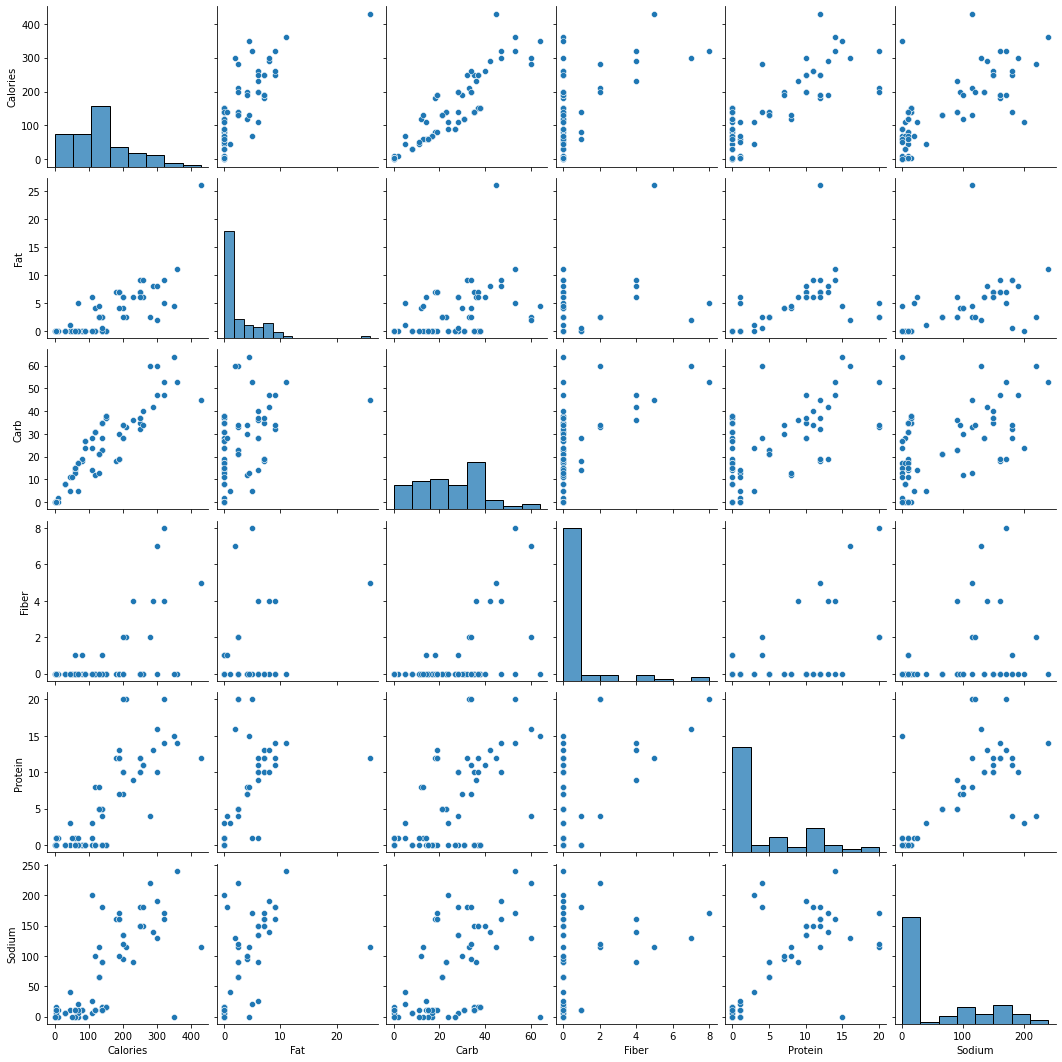
\includegraphics{Data visualization_files/figure-pdf/cell-43-output-1.png}

}

\end{figure}

\hypertarget{histgram-1}{%
\subsubsection{Histgram}\label{histgram-1}}

\begin{Shaded}
\begin{Highlighting}[]
\NormalTok{sns.histplot(data}\OperatorTok{=}\NormalTok{flowers\_df, x}\OperatorTok{=}\StringTok{\textquotesingle{}sepal\_width\textquotesingle{}}\NormalTok{)}\OperatorTok{;}
\end{Highlighting}
\end{Shaded}

\begin{figure}[H]

{\centering 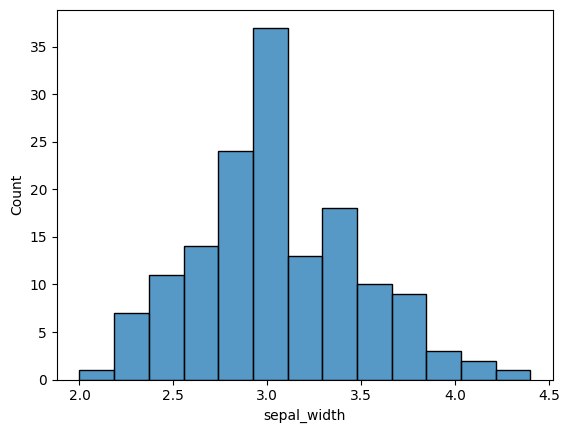
\includegraphics{Data visualization_files/figure-pdf/cell-44-output-1.png}

}

\end{figure}

\begin{Shaded}
\begin{Highlighting}[]
\CommentTok{\# show kde(kernal density estimate)}
\NormalTok{sns.histplot(data}\OperatorTok{=}\NormalTok{flowers\_df, x}\OperatorTok{=}\StringTok{\textquotesingle{}sepal\_width\textquotesingle{}}\NormalTok{, kde}\OperatorTok{=}\VariableTok{True}\NormalTok{)}\OperatorTok{;}
\end{Highlighting}
\end{Shaded}

\begin{figure}[H]

{\centering 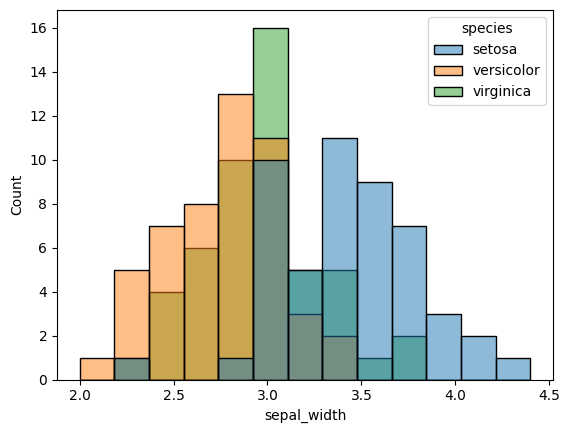
\includegraphics{Data visualization_files/figure-pdf/cell-45-output-1.png}

}

\end{figure}

\begin{Shaded}
\begin{Highlighting}[]
\CommentTok{\# adding hue}
\NormalTok{sns.histplot(data}\OperatorTok{=}\NormalTok{flowers\_df, x}\OperatorTok{=}\StringTok{"sepal\_width"}\NormalTok{, hue}\OperatorTok{=}\StringTok{"species"}\NormalTok{)}\OperatorTok{;}
\end{Highlighting}
\end{Shaded}

\begin{figure}[H]

{\centering 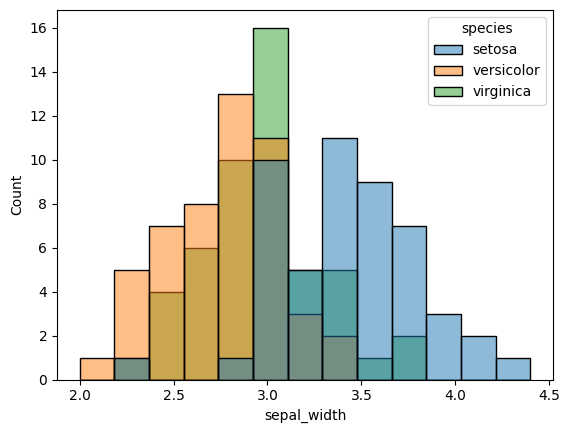
\includegraphics{Data visualization_files/figure-pdf/cell-46-output-1.png}

}

\end{figure}

\hypertarget{barplot}{%
\subsubsection{Barplot}\label{barplot}}

\begin{Shaded}
\begin{Highlighting}[]
\NormalTok{tips\_df }\OperatorTok{=}\NormalTok{ sns.load\_dataset(}\StringTok{"tips"}\NormalTok{)}
\NormalTok{sns.barplot(x}\OperatorTok{=}\StringTok{\textquotesingle{}day\textquotesingle{}}\NormalTok{, y}\OperatorTok{=}\StringTok{\textquotesingle{}total\_bill\textquotesingle{}}\NormalTok{, data}\OperatorTok{=}\NormalTok{tips\_df)}\OperatorTok{;}
\end{Highlighting}
\end{Shaded}

\begin{figure}[H]

{\centering 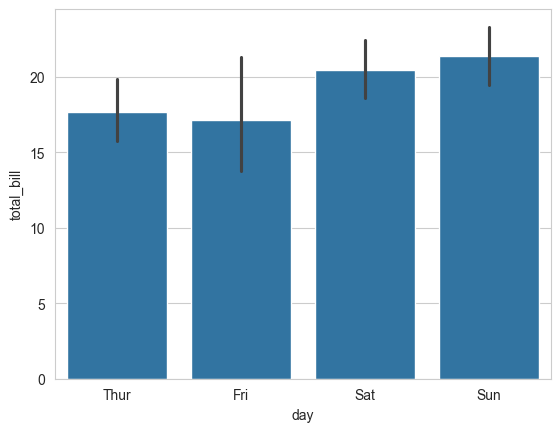
\includegraphics{Data visualization_files/figure-pdf/cell-47-output-1.png}

}

\end{figure}

\begin{Shaded}
\begin{Highlighting}[]
\NormalTok{sns.barplot(x}\OperatorTok{=}\StringTok{\textquotesingle{}day\textquotesingle{}}\NormalTok{, y}\OperatorTok{=}\StringTok{\textquotesingle{}tip\textquotesingle{}}\NormalTok{, hue}\OperatorTok{=}\StringTok{\textquotesingle{}sex\textquotesingle{}}\NormalTok{, data}\OperatorTok{=}\NormalTok{tips\_df)}\OperatorTok{;}
\end{Highlighting}
\end{Shaded}

\begin{figure}[H]

{\centering 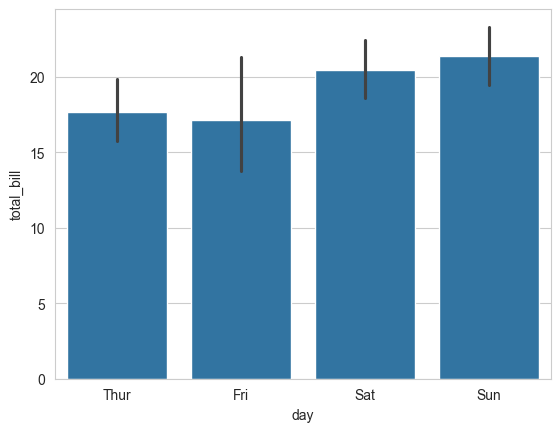
\includegraphics{Data visualization_files/figure-pdf/cell-48-output-1.png}

}

\end{figure}

\begin{Shaded}
\begin{Highlighting}[]
\CommentTok{\# make the bars horizontal simply by switching the axes}
\NormalTok{sns.barplot(x}\OperatorTok{=}\StringTok{\textquotesingle{}tip\textquotesingle{}}\NormalTok{, y}\OperatorTok{=}\StringTok{\textquotesingle{}day\textquotesingle{}}\NormalTok{, hue}\OperatorTok{=}\StringTok{\textquotesingle{}sex\textquotesingle{}}\NormalTok{, data}\OperatorTok{=}\NormalTok{tips\_df)}\OperatorTok{;}
\end{Highlighting}
\end{Shaded}

\begin{figure}[H]

{\centering 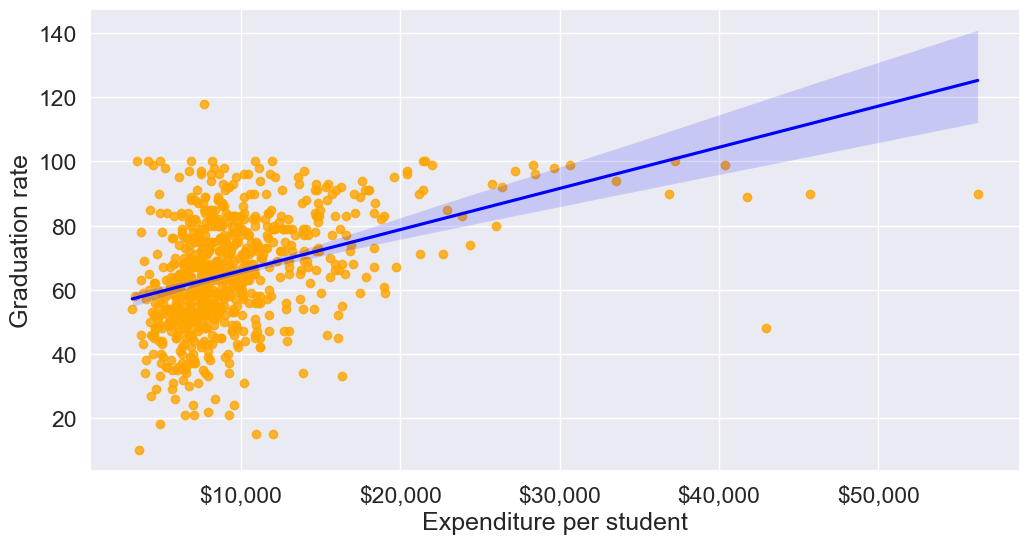
\includegraphics{Data visualization_files/figure-pdf/cell-49-output-1.png}

}

\end{figure}

\hypertarget{boxplot}{%
\subsubsection{Boxplot}\label{boxplot}}

\textbf{Purpose:} Boxplots is a standardized way of visualizing the
distribution of a continuous variable. They show five key metrics that
describe the data distribution - median, 25th percentile value, 75th
percentile value, minimum and maximum, as shown in the figure below.
Note that the minimum and maximum exclude the outliers.

\begin{verbatim}
<IPython.core.display.Image object>
\end{verbatim}

\textbf{Example:} Create a box plot to compare the distributions of
total tips based on the day of the week, differentiating between male
and female patrons.

\begin{Shaded}
\begin{Highlighting}[]
\NormalTok{sns.boxplot(data}\OperatorTok{=}\NormalTok{tips\_df, y}\OperatorTok{=}\StringTok{\textquotesingle{}total\_bill\textquotesingle{}}\NormalTok{, x}\OperatorTok{=}\StringTok{\textquotesingle{}day\textquotesingle{}}\NormalTok{, hue}\OperatorTok{=}\StringTok{\textquotesingle{}sex\textquotesingle{}}\NormalTok{)}\OperatorTok{;}
\end{Highlighting}
\end{Shaded}

\begin{figure}[H]

{\centering 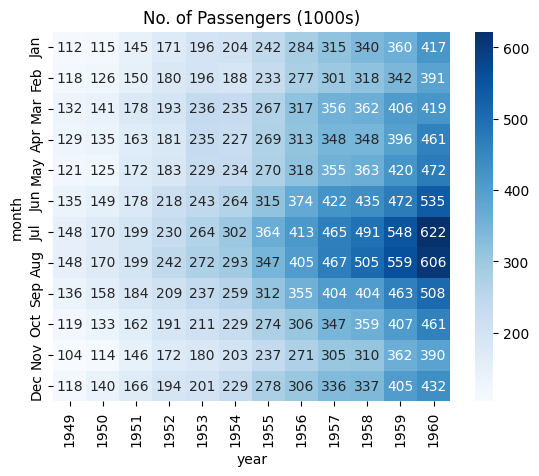
\includegraphics{Data visualization_files/figure-pdf/cell-51-output-1.png}

}

\end{figure}

From the above plot, what you can observe?

\hypertarget{heatmap}{%
\subsubsection{Heatmap}\label{heatmap}}

Represent 2-dimensional data like a matrix or table using colors

\begin{Shaded}
\begin{Highlighting}[]
\NormalTok{flights\_df }\OperatorTok{=}\NormalTok{ sns.load\_dataset(}\StringTok{"flights"}\NormalTok{).pivot(index}\OperatorTok{=}\StringTok{"month"}\NormalTok{, columns}\OperatorTok{=}\StringTok{"year"}\NormalTok{, values}\OperatorTok{=}\StringTok{"passengers"}\NormalTok{)}
\NormalTok{flights\_df}
\CommentTok{\# you will learn pivot in the later chapters}
\end{Highlighting}
\end{Shaded}

\begin{longtable}[]{@{}lllllllllllll@{}}
\toprule\noalign{}
year & 1949 & 1950 & 1951 & 1952 & 1953 & 1954 & 1955 & 1956 & 1957 &
1958 & 1959 & 1960 \\
month & & & & & & & & & & & & \\
\midrule\noalign{}
\endhead
\bottomrule\noalign{}
\endlastfoot
Jan & 112 & 115 & 145 & 171 & 196 & 204 & 242 & 284 & 315 & 340 & 360 &
417 \\
Feb & 118 & 126 & 150 & 180 & 196 & 188 & 233 & 277 & 301 & 318 & 342 &
391 \\
Mar & 132 & 141 & 178 & 193 & 236 & 235 & 267 & 317 & 356 & 362 & 406 &
419 \\
Apr & 129 & 135 & 163 & 181 & 235 & 227 & 269 & 313 & 348 & 348 & 396 &
461 \\
May & 121 & 125 & 172 & 183 & 229 & 234 & 270 & 318 & 355 & 363 & 420 &
472 \\
Jun & 135 & 149 & 178 & 218 & 243 & 264 & 315 & 374 & 422 & 435 & 472 &
535 \\
Jul & 148 & 170 & 199 & 230 & 264 & 302 & 364 & 413 & 465 & 491 & 548 &
622 \\
Aug & 148 & 170 & 199 & 242 & 272 & 293 & 347 & 405 & 467 & 505 & 559 &
606 \\
Sep & 136 & 158 & 184 & 209 & 237 & 259 & 312 & 355 & 404 & 404 & 463 &
508 \\
Oct & 119 & 133 & 162 & 191 & 211 & 229 & 274 & 306 & 347 & 359 & 407 &
461 \\
Nov & 104 & 114 & 146 & 172 & 180 & 203 & 237 & 271 & 305 & 310 & 362 &
390 \\
Dec & 118 & 140 & 166 & 194 & 201 & 229 & 278 & 306 & 336 & 337 & 405 &
432 \\
\end{longtable}

\texttt{flights\_df} is a matrix with one row for each month and one
column for each year. The values show the number of passengers (in
thousands) that visited the airport in a specific month of a year. We
can use the \texttt{sns.heatmap} function to visualize the footfall at
the airport.

\begin{Shaded}
\begin{Highlighting}[]
\NormalTok{plt.title(}\StringTok{"No. of Passengers (1000s)"}\NormalTok{)}
\NormalTok{sns.heatmap(flights\_df)}\OperatorTok{;}
\end{Highlighting}
\end{Shaded}

\begin{figure}[H]

{\centering 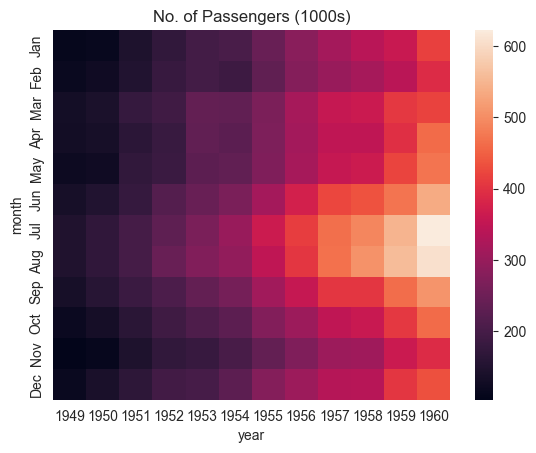
\includegraphics{Data visualization_files/figure-pdf/cell-53-output-1.png}

}

\end{figure}

The brighter colors indicate a higher footfall at the airport. By
looking at the graph, we can infer two things:

\begin{itemize}
\tightlist
\item
  The footfall at the airport in any given year tends to be the highest
  around July \& August.
\item
  The footfall at the airport in any given month tends to grow year by
  year.
\end{itemize}

We can also display the actual values in each block by specifying
\texttt{annot=True} and using the \texttt{cmap} argument to change the
color palette.

\begin{Shaded}
\begin{Highlighting}[]
\CommentTok{\# fmt = "d" decimal integer. output are the number in base 10}
\NormalTok{plt.title(}\StringTok{"No. of Passengers (1000s)"}\NormalTok{)}
\NormalTok{sns.heatmap(flights\_df, fmt}\OperatorTok{=}\StringTok{"d"}\NormalTok{, annot}\OperatorTok{=}\VariableTok{True}\NormalTok{, cmap}\OperatorTok{=}\StringTok{\textquotesingle{}Blues\textquotesingle{}}\NormalTok{)}\OperatorTok{;}
\end{Highlighting}
\end{Shaded}

\begin{figure}[H]

{\centering 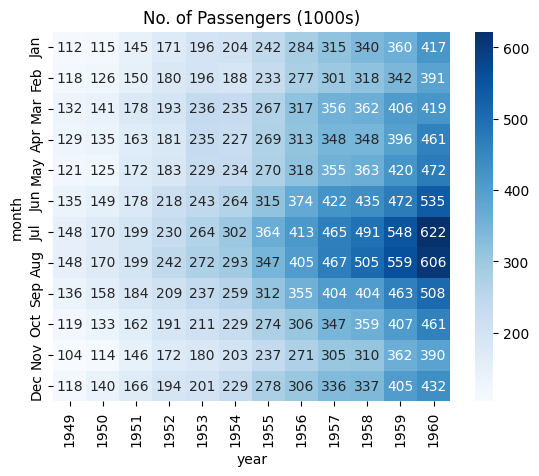
\includegraphics{Data visualization_files/figure-pdf/cell-54-output-1.png}

}

\end{figure}

\hypertarget{correlation-map}{%
\subsubsection{Correlation Map}\label{correlation-map}}

A correlation map is a specific type of heatmap where the values
represent the correlation coefficients between variables (ranging from
-1 to 1). It visually shows the strength and direction of relationships
between numerical variables.

Correlation may refer to any kind of association between two random
variables. However, in this book, we will always consider correlation as
the linear association between two random variables, or the Pearson's
correlation coefficient. Note that correlation does not imply causality
and vice-versa.

The Pandas function
\href{https://pandas.pydata.org/docs/reference/api/pandas.DataFrame.corr.html}{corr()}
provides the pairwise correlation between all columns of a DataFrame, or
between two Series. The function
\href{https://pandas.pydata.org/docs/reference/api/pandas.DataFrame.corrwith.html\#pandas.DataFrame.corrwith}{corrwith()}
provides the pairwise correlation of a DataFrame with another DataFrame
or Series.

\begin{Shaded}
\begin{Highlighting}[]
\CommentTok{\#Pairwise correlation amongst all columns}
\NormalTok{survey\_data }\OperatorTok{=}\NormalTok{ pd.read\_csv(}\StringTok{\textquotesingle{}./Datasets/survey\_data\_clean.csv\textquotesingle{}}\NormalTok{)}

\NormalTok{survey\_data.head()}
\end{Highlighting}
\end{Shaded}

\begin{longtable}[]{@{}llllllllllllllllllllll@{}}
\toprule\noalign{}
& Timestamp & fav\_alcohol & parties\_per\_month & smoke & weed &
introvert\_extrovert & love\_first\_sight & learning\_style &
left\_right\_brained & personality\_type & ... & used\_python\_before &
dominant\_hand & childhood\_in\_US & gender & region\_of\_residence &
political\_affliation & cant\_change\_math\_ability &
can\_change\_math\_ability & math\_is\_genetic &
much\_effort\_is\_lack\_of\_talent \\
\midrule\noalign{}
\endhead
\bottomrule\noalign{}
\endlastfoot
0 & 2022/09/13 1:43:34 pm GMT-5 & I don\textquotesingle t drink & 1.0 &
No & Occasionally & Introvert & 0 & Visual (learn best through images or
graphic o... & Left-brained (logic, science, critical thinkin... & INFJ
& ... & 1 & Right & 1 & Female & Northeast & Democrat & 0 & 1 & 0 & 0 \\
1 & 2022/09/13 5:28:17 pm GMT-5 & Hard liquor/Mixed drink & 3.0 & No &
Occasionally & Extrovert & 0 & Visual (learn best through images or
graphic o... & Left-brained (logic, science, critical thinkin... & ESFJ
& ... & 1 & Right & 1 & Male & West & Democrat & 0 & 1 & 0 & 0 \\
2 & 2022/09/13 7:56:38 pm GMT-5 & Hard liquor/Mixed drink & 3.0 & No &
Yes & Introvert & 0 & Kinesthetic (learn best through figuring out h...
& Left-brained (logic, science, critical thinkin... & ISTJ & ... & 0 &
Right & 0 & Female & International & No affiliation & 0 & 1 & 0 & 0 \\
3 & 2022/09/13 10:34:37 pm GMT-5 & Hard liquor/Mixed drink & 12.0 & No &
No & Extrovert & 0 & Visual (learn best through images or graphic o... &
Left-brained (logic, science, critical thinkin... & ENFJ & ... & 0 &
Right & 1 & Female & Southeast & Democrat & 0 & 1 & 0 & 0 \\
4 & 2022/09/14 4:46:19 pm GMT-5 & I don\textquotesingle t drink & 1.0 &
No & No & Extrovert & 1 & Reading/Writing (learn best through words
ofte... & Right-brained (creative, art, imaginative, int... & ENTJ & ...
& 0 & Right & 1 & Female & Northeast & Democrat & 1 & 0 & 0 & 0 \\
\end{longtable}

\begin{Shaded}
\begin{Highlighting}[]
\CommentTok{\#Pairwise correlation amongst all columns}
\NormalTok{survey\_data.select\_dtypes(include}\OperatorTok{=}\StringTok{\textquotesingle{}number\textquotesingle{}}\NormalTok{).corr()}
\end{Highlighting}
\end{Shaded}

\begin{longtable}[]{@{}llllllllllllllllllllll@{}}
\toprule\noalign{}
& parties\_per\_month & love\_first\_sight & num\_insta\_followers &
expected\_marriage\_age & expected\_starting\_salary &
minutes\_ex\_per\_week & sleep\_hours\_per\_day &
farthest\_distance\_travelled & fav\_number & internet\_hours\_per\_day
& ... & procrastinator & num\_clubs & student\_athlete & AP\_stats &
used\_python\_before & childhood\_in\_US & cant\_change\_math\_ability &
can\_change\_math\_ability & math\_is\_genetic &
much\_effort\_is\_lack\_of\_talent \\
\midrule\noalign{}
\endhead
\bottomrule\noalign{}
\endlastfoot
parties\_per\_month & 1.000000 & 0.096129 & 0.239705 & -0.064079 &
0.114881 & 0.195561 & -0.052542 & -0.017081 & -0.050139 & 0.087390 & ...
& -0.056871 & -0.010514 & 0.290830 & -0.013222 & -0.040033 & 0.081905 &
-0.052912 & 0.055575 & -0.013374 & -0.029838 \\
love\_first\_sight & 0.096129 & 1.000000 & -0.024010 & -0.084406 &
0.080138 & 0.099244 & -0.025378 & -0.075539 & 0.105095 & -0.007652 & ...
& 0.033951 & 0.083342 & 0.014595 & -0.062992 & -0.034692 & -0.118260 &
0.005254 & 0.020758 & -0.003710 & 0.013376 \\
num\_insta\_followers & 0.239705 & -0.024010 & 1.000000 & -0.130157 &
0.127226 & 0.099341 & -0.042421 & 0.011308 & -0.124763 & -0.028427 & ...
& -0.089871 & 0.265958 & 0.044807 & 0.005947 & -0.016201 & 0.072622 &
-0.150658 & 0.130774 & -0.018411 & -0.165899 \\
expected\_marriage\_age & -0.064079 & -0.084406 & -0.130157 & 1.000000 &
-0.014881 & -0.088073 & 0.182009 & -0.024038 & -0.008924 & -0.029772 &
... & -0.020012 & -0.137069 & -0.036122 & 0.010447 & 0.052727 & 0.053759
& -0.072163 & 0.087633 & -0.086898 & 0.052813 \\
expected\_starting\_salary & 0.114881 & 0.080138 & 0.127226 & -0.014881
& 1.000000 & 0.134065 & -0.005078 & -0.028329 & -0.028125 & 0.017479 &
... & 0.054273 & -0.100922 & -0.026219 & -0.084894 & -0.094541 &
0.081142 & -0.011609 & 0.019171 & 0.078694 & 0.097265 \\
minutes\_ex\_per\_week & 0.195561 & 0.099244 & 0.099341 & -0.088073 &
0.134065 & 1.000000 & 0.049593 & -0.153188 & 0.038758 & -0.028457 & ...
& -0.045149 & -0.024572 & 0.576301 & -0.062544 & 0.057760 & 0.235492 &
-0.101282 & 0.134430 & -0.047772 & -0.045141 \\
sleep\_hours\_per\_day & -0.052542 & -0.025378 & -0.042421 & 0.182009 &
-0.005078 & 0.049593 & 1.000000 & 0.104175 & -0.021909 & 0.017435 & ...
& -0.176579 & -0.163860 & 0.058361 & -0.013909 & 0.096528 & -0.059468 &
-0.058086 & 0.012174 & 0.027052 & -0.022025 \\
farthest\_distance\_travelled & -0.017081 & -0.075539 & 0.011308 &
-0.024038 & -0.028329 & -0.153188 & 0.104175 & 1.000000 & -0.108661 &
0.049450 & ... & 0.032492 & -0.045214 & -0.158027 & 0.010580 & 0.012353
& -0.282821 & -0.046074 & 0.017935 & 0.110037 & 0.046895 \\
fav\_number & -0.050139 & 0.105095 & -0.124763 & -0.008924 & -0.028125 &
0.038758 & -0.021909 & -0.108661 & 1.000000 & -0.013070 & ... & 0.085508
& -0.013696 & -0.014435 & 0.091011 & 0.030736 & 0.072894 & -0.032534 &
0.034319 & -0.063692 & -0.073777 \\
internet\_hours\_per\_day & 0.087390 & -0.007652 & -0.028427 & -0.029772
& 0.017479 & -0.028457 & 0.017435 & 0.049450 & -0.013070 & 1.000000 &
... & 0.048239 & 0.064527 & -0.017944 & 0.001818 & 0.051970 & 0.033120 &
-0.033902 & 0.050258 & 0.190205 & -0.053708 \\
only\_child & -0.142519 & 0.124345 & -0.152184 & -0.043141 & -0.088648 &
-0.123371 & 0.038126 & 0.214377 & -0.024419 & -0.035022 & ... & 0.073415
& -0.065484 & 0.064136 & 0.048031 & -0.139898 & -0.387711 & 0.023089 &
-0.019982 & 0.058226 & 0.092372 \\
num\_majors\_minors & -0.073127 & 0.108730 & 0.050431 & -0.055280 &
0.021278 & 0.044450 & -0.024339 & -0.012779 & 0.023903 & -0.073775 & ...
& -0.073806 & 0.311266 & -0.035500 & -0.068640 & -0.073388 & -0.153529 &
-0.077501 & 0.024734 & -0.125809 & -0.064939 \\
high\_school\_GPA & 0.295646 & 0.069288 & 0.147402 & 0.017052 & 0.053354
& -0.076471 & -0.036904 & -0.064116 & -0.023081 & -0.034485 & ... &
0.031561 & -0.020854 & 0.006332 & 0.066837 & 0.072777 & 0.005606 &
-0.095025 & 0.093416 & -0.082620 & 0.001373 \\
NU\_GPA & -0.080548 & -0.114041 & 0.004702 & 0.011925 & -0.048069 &
-0.108177 & 0.143997 & 0.038238 & -0.307656 & -0.014531 & ... &
-0.269552 & 0.016724 & -0.027378 & -0.026544 & -0.008536 & -0.028968 &
0.002094 & -0.137330 & 0.036731 & 0.047840 \\
age & -0.032771 & 0.142384 & -0.230698 & 0.060416 & -0.102632 &
-0.040906 & -0.035890 & 0.018811 & 0.096818 & 0.017515 & ... & -0.005892
& -0.127760 & -0.038315 & -0.026959 & 0.009924 & -0.152784 & -0.005954 &
0.014759 & -0.009315 & -0.126370 \\
height & -0.005405 & 0.216072 & 0.009318 & 0.044577 & 0.151517 &
0.182090 & -0.010650 & -0.235067 & 0.041298 & -0.023174 & ... & 0.063263
& 0.212038 & 0.080953 & 0.022484 & 0.016110 & 0.160309 & -0.055641 &
0.101811 & -0.064383 & 0.028509 \\
height\_father & 0.126741 & 0.029419 & 0.179684 & 0.026949 & 0.011450 &
0.156227 & 0.097593 & -0.118669 & -0.032717 & -0.047314 & ... &
-0.111183 & 0.022701 & 0.155003 & -0.010982 & -0.006480 & 0.137934 &
-0.019593 & 0.008157 & 0.010222 & 0.060439 \\
height\_mother & 0.079121 & 0.082684 & 0.129716 & 0.075316 & 0.033947 &
0.114181 & -0.044089 & -0.134582 & -0.029568 & -0.091417 & ... &
-0.078265 & 0.091390 & 0.053258 & -0.100647 & -0.021396 & 0.119292 &
0.027120 & 0.034961 & -0.035449 & 0.074492 \\
procrastinator & -0.056871 & 0.033951 & -0.089871 & -0.020012 & 0.054273
& -0.045149 & -0.176579 & 0.032492 & 0.085508 & 0.048239 & ... &
1.000000 & 0.078341 & 0.094363 & 0.003053 & -0.016254 & -0.090868 &
0.002462 & 0.084419 & -0.001738 & 0.081471 \\
num\_clubs & -0.010514 & 0.083342 & 0.265958 & -0.137069 & -0.100922 &
-0.024572 & -0.163860 & -0.045214 & -0.013696 & 0.064527 & ... &
0.078341 & 1.000000 & -0.084562 & 0.087438 & 0.115062 & -0.021044 &
-0.136249 & 0.070002 & -0.090570 & -0.108851 \\
student\_athlete & 0.290830 & 0.014595 & 0.044807 & -0.036122 &
-0.026219 & 0.576301 & 0.058361 & -0.158027 & -0.014435 & -0.017944 &
... & 0.094363 & -0.084562 & 1.000000 & -0.040686 & -0.049288 & 0.082888
& -0.066667 & -0.022576 & -0.060523 & 0.121232 \\
AP\_stats & -0.013222 & -0.062992 & 0.005947 & 0.010447 & -0.084894 &
-0.062544 & -0.013909 & 0.010580 & 0.091011 & 0.001818 & ... & 0.003053
& 0.087438 & -0.040686 & 1.000000 & 0.089517 & 0.106584 & 0.081109 &
0.029743 & -0.048375 & -0.018043 \\
used\_python\_before & -0.040033 & -0.034692 & -0.016201 & 0.052727 &
-0.094541 & 0.057760 & 0.096528 & 0.012353 & 0.030736 & 0.051970 & ... &
-0.016254 & 0.115062 & -0.049288 & 0.089517 & 1.000000 & 0.041928 &
-0.011217 & 0.156806 & 0.088566 & 0.023366 \\
childhood\_in\_US & 0.081905 & -0.118260 & 0.072622 & 0.053759 &
0.081142 & 0.235492 & -0.059468 & -0.282821 & 0.072894 & 0.033120 & ...
& -0.090868 & -0.021044 & 0.082888 & 0.106584 & 0.041928 & 1.000000 &
-0.008575 & 0.057185 & -0.178003 & -0.013098 \\
cant\_change\_math\_ability & -0.052912 & 0.005254 & -0.150658 &
-0.072163 & -0.011609 & -0.101282 & -0.058086 & -0.046074 & -0.032534 &
-0.033902 & ... & 0.002462 & -0.136249 & -0.066667 & 0.081109 &
-0.011217 & -0.008575 & 1.000000 & -0.672777 & 0.294544 & 0.101835 \\
can\_change\_math\_ability & 0.055575 & 0.020758 & 0.130774 & 0.087633 &
0.019171 & 0.134430 & 0.012174 & 0.017935 & 0.034319 & 0.050258 & ... &
0.084419 & 0.070002 & -0.022576 & 0.029743 & 0.156806 & 0.057185 &
-0.672777 & 1.000000 & -0.361546 & -0.131047 \\
math\_is\_genetic & -0.013374 & -0.003710 & -0.018411 & -0.086898 &
0.078694 & -0.047772 & 0.027052 & 0.110037 & -0.063692 & 0.190205 & ...
& -0.001738 & -0.090570 & -0.060523 & -0.048375 & 0.088566 & -0.178003 &
0.294544 & -0.361546 & 1.000000 & 0.154083 \\
much\_effort\_is\_lack\_of\_talent & -0.029838 & 0.013376 & -0.165899 &
0.052813 & 0.097265 & -0.045141 & -0.022025 & 0.046895 & -0.073777 &
-0.053708 & ... & 0.081471 & -0.108851 & 0.121232 & -0.018043 & 0.023366
& -0.013098 & 0.101835 & -0.131047 & 0.154083 & 1.000000 \\
\end{longtable}

\textbf{Q:} Which feature is the most correlated with \emph{NU\_GPA}?

\begin{Shaded}
\begin{Highlighting}[]
\NormalTok{survey\_data.select\_dtypes(include}\OperatorTok{=}\StringTok{\textquotesingle{}number\textquotesingle{}}\NormalTok{).corrwith(survey\_data.NU\_GPA).sort\_values(ascending }\OperatorTok{=} \VariableTok{False}\NormalTok{)}
\end{Highlighting}
\end{Shaded}

\begin{verbatim}
NU_GPA                           1.000000
sleep_hours_per_day              0.143997
num_majors_minors                0.141988
only_child                       0.106440
much_effort_is_lack_of_talent    0.047840
farthest_distance_travelled      0.038238
math_is_genetic                  0.036731
num_clubs                        0.016724
expected_marriage_age            0.011925
num_insta_followers              0.004702
cant_change_math_ability         0.002094
used_python_before              -0.008536
internet_hours_per_day          -0.014531
AP_stats                        -0.026544
student_athlete                 -0.027378
childhood_in_US                 -0.028968
high_school_GPA                 -0.030883
height_father                   -0.040120
expected_starting_salary        -0.048069
age                             -0.052039
height_mother                   -0.079276
parties_per_month               -0.080548
height                          -0.099082
minutes_ex_per_week             -0.108177
love_first_sight                -0.114041
can_change_math_ability         -0.137330
procrastinator                  -0.269552
fav_number                      -0.307656
dtype: float64
\end{verbatim}

\begin{Shaded}
\begin{Highlighting}[]
\NormalTok{sns.}\BuiltInTok{set}\NormalTok{(rc}\OperatorTok{=}\NormalTok{\{}\StringTok{\textquotesingle{}figure.figsize\textquotesingle{}}\NormalTok{:(}\DecValTok{12}\NormalTok{,}\DecValTok{10}\NormalTok{)\})}
\NormalTok{sns.heatmap(survey\_data.select\_dtypes(include}\OperatorTok{=}\StringTok{\textquotesingle{}number\textquotesingle{}}\NormalTok{).corr())}\OperatorTok{;}
\end{Highlighting}
\end{Shaded}

\begin{figure}[H]

{\centering 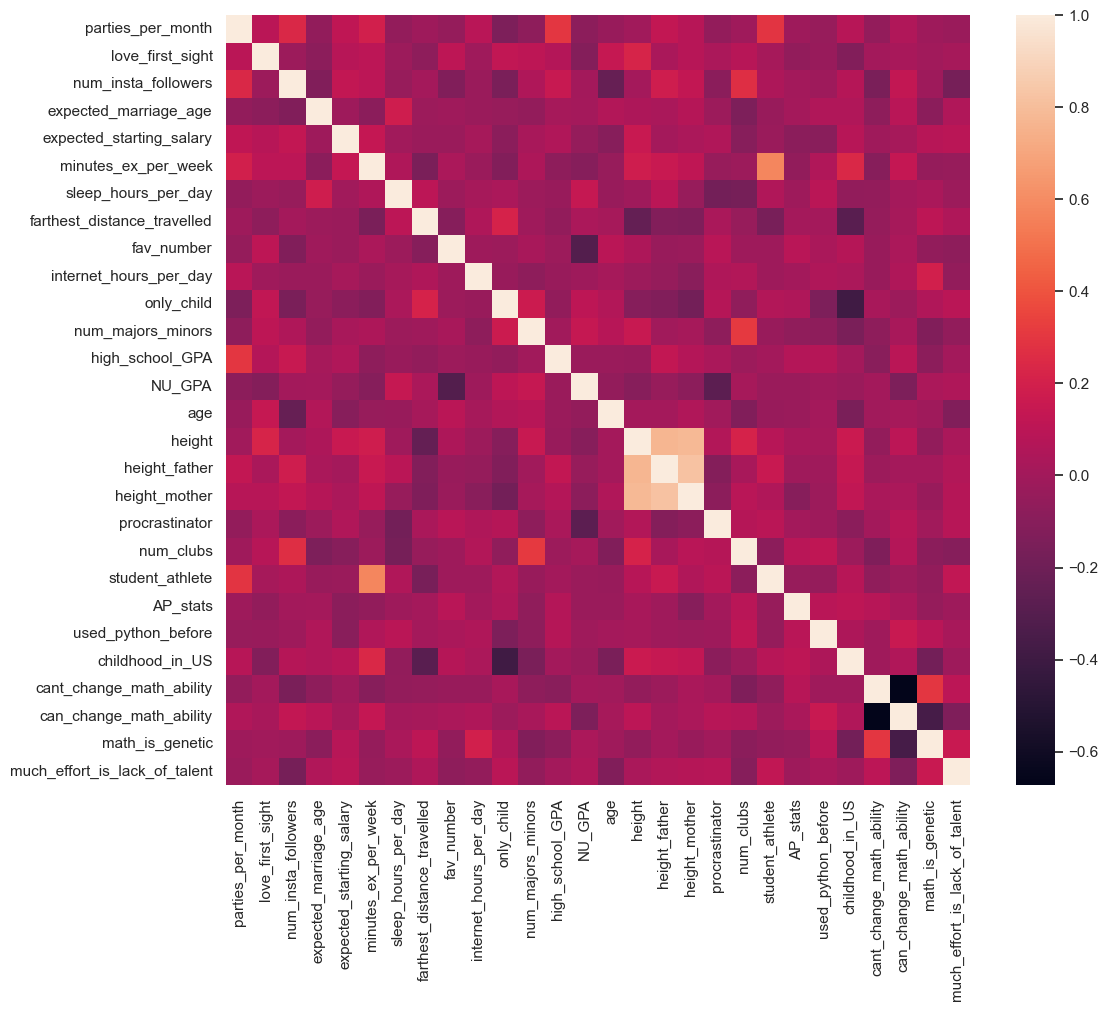
\includegraphics{Data visualization_files/figure-pdf/cell-58-output-1.png}

}

\end{figure}

From the above map, we can see that:

\begin{itemize}
\tightlist
\item
  \texttt{student\ athlete} is strongly postively correlated with
  \texttt{minutes\_ex\_per\_week}
\item
  \texttt{procrastinator} is strongly negatively correlated with
  \texttt{NU\_GPA}
\end{itemize}

\hypertarget{independent-study}{%
\section{Independent Study}\label{independent-study}}

\hypertarget{practice-exercise-1-3}{%
\subsection{Practice exercise 1}\label{practice-exercise-1-3}}

Read the \emph{gas\_price.csv} file and plot the trend for each country
over the time using matplotlib \texttt{pyplot}

\hypertarget{practice-exercise-2-3}{%
\subsection{Practice exercise 2}\label{practice-exercise-2-3}}

\hypertarget{section-39}{%
\subsubsection{}\label{section-39}}

Is \texttt{NU\_GPA} associated with \texttt{parties\_per\_month}?
Analyze the association separately for \emph{Sophomores, Juniors, and
Seniors} (categories of the variable \texttt{school\_year}).

Make scatterplots of \texttt{NU\_GPA} vs \texttt{parties\_per\_month} in
a 1 x 3 grid, where each grid is for a distinct \texttt{school\_year}.
Plot the trendline as well for each scatterplot. Use the file
\emph{survey\_data\_clean.csv}.

\hypertarget{section-40}{%
\subsubsection{}\label{section-40}}

Capping the the values of \texttt{parties\_per\_month} to 30, and make
the visualizations again.

\hypertarget{practice-exercise-3-3}{%
\subsection{Practice exercise 3}\label{practice-exercise-3-3}}

How does the expected marriage age of the people of STAT303-1 depend on
their characteristics? We'll use visualizations to answer this question.
Use data from the file \emph{survey\_data\_clean.csv.} Proceed as
follows:

\hypertarget{section-41}{%
\subsubsection{}\label{section-41}}

Make a visualization that compares the mean
\texttt{expected\_marriage\_age} of introverts and extroverts \emph{(use
the variable \texttt{introvert\_extrovert})}. What insights do you
obtain?

\hypertarget{section-42}{%
\subsubsection{}\label{section-42}}

Does the mean \texttt{expected\_marriage\_age} of introverts and
extroverts depend on whether they believe in love in first sight
\emph{(variable name: \texttt{love\_first\_sight})}? Update the previous
visualization to answer the question.

\hypertarget{section-43}{%
\subsubsection{}\label{section-43}}

In addition to \texttt{love\_first\_sight}, does the mean
\texttt{expected\_marriage\_age} of introverts and extroverts depend on
whether they are a procrastinator \emph{(variable name:
\texttt{procrastinator})}? Update the previous visualization to answer
the question.

\hypertarget{section-44}{%
\subsubsection{}\label{section-44}}

Is there any critical information missing in the above visualizations
that, if revealed, may cast doubts on the patterns observed in them?

\hypertarget{practice-exercise-4-2}{%
\subsection{Practice exercise 4}\label{practice-exercise-4-2}}

Read \emph{Australia\_weather.csv},

\hypertarget{section-45}{%
\subsubsection{}\label{section-45}}

Create a histogram showing the distributions of maximum temperature in
Sydney, Canberra and Melbourne.

\hypertarget{section-46}{%
\subsubsection{}\label{section-46}}

Make a density plot showing the distributions of maximum temperature in
Sydney, Canberra and Melbourne.

\hypertarget{section-47}{%
\subsubsection{}\label{section-47}}

Show the distributions of the maximum and minimum temperatures in a
single plot.

\hypertarget{section-48}{%
\subsubsection{}\label{section-48}}

Create a scatter plot with a trendline for \texttt{MinTemp} and
\texttt{MaxTemp}, including a confidence interval.

\textbf{Hint}: Using Seaborn, the \texttt{regplot()} function enables us
to overlay a trendline on the scatter plot, complete with a 95\%
confidence interval for the trendline

\hypertarget{advanced-data-visualization}{%
\chapter{Advanced Data
Visualization}\label{advanced-data-visualization}}

In the previous chapter, we explored basic plotting techniques using
Pandas, Seaborn, and Matplotlib to create visualizations. Now, we'll
elevate our skills by diving into more advanced topics, such as crafting
complex subplots and visualizing geospatial data, enabling us to build
richer and more insightful plots.

To get started, let's import necessary libraries.

\begin{Shaded}
\begin{Highlighting}[]
\ImportTok{import}\NormalTok{ pandas }\ImportTok{as}\NormalTok{ pd}
\ImportTok{import}\NormalTok{ numpy }\ImportTok{as}\NormalTok{ np}
\ImportTok{import}\NormalTok{ matplotlib.pyplot }\ImportTok{as}\NormalTok{ plt}
\ImportTok{import}\NormalTok{ seaborn }\ImportTok{as}\NormalTok{ sns}

\OperatorTok{\%}\NormalTok{matplotlib inline}
\end{Highlighting}
\end{Shaded}

\hypertarget{matplotlib-plotting-interfaces}{%
\section{Matplotlib Plotting
Interfaces}\label{matplotlib-plotting-interfaces}}

\hypertarget{pyplot-interface-and-oop-interface}{%
\subsection{Pyplot interface and OOP
Interface}\label{pyplot-interface-and-oop-interface}}

There are two types of interfaces in Matplotlib for visualization and
these are given below:

\includegraphics{https://s3.ap-south-1.amazonaws.com/s3.studytonight.com/tutorials/uploads/pictures/1596086186-71449.png}

\hypertarget{plot-a-simple-figure-using-two-interfaces}{%
\subsection{Plot a simple figure using two
interfaces}\label{plot-a-simple-figure-using-two-interfaces}}

\begin{Shaded}
\begin{Highlighting}[]
\NormalTok{gdp\_data }\OperatorTok{=}\NormalTok{ pd.read\_csv(}\StringTok{\textquotesingle{}datasets/gdp\_lifeExpectancy.csv\textquotesingle{}}\NormalTok{)}
\NormalTok{gdp\_data.head()}
\end{Highlighting}
\end{Shaded}

\begin{longtable}[]{@{}lllllll@{}}
\toprule\noalign{}
& country & continent & year & lifeExp & pop & gdpPercap \\
\midrule\noalign{}
\endhead
\bottomrule\noalign{}
\endlastfoot
0 & Afghanistan & Asia & 1952 & 28.801 & 8425333 & 779.445314 \\
1 & Afghanistan & Asia & 1957 & 30.332 & 9240934 & 820.853030 \\
2 & Afghanistan & Asia & 1962 & 31.997 & 10267083 & 853.100710 \\
3 & Afghanistan & Asia & 1967 & 34.020 & 11537966 & 836.197138 \\
4 & Afghanistan & Asia & 1972 & 36.088 & 13079460 & 739.981106 \\
\end{longtable}

\begin{Shaded}
\begin{Highlighting}[]
\CommentTok{\#Object{-}oriented interface}
\NormalTok{fig, ax }\OperatorTok{=}\NormalTok{ plt.subplots() }\CommentTok{\#Create a figure and an axes}
\NormalTok{x }\OperatorTok{=}\NormalTok{ gdp\_data.gdpPercap }
\NormalTok{y }\OperatorTok{=}\NormalTok{ gdp\_data.lifeExp}
\NormalTok{ax.plot(x,y,}\StringTok{\textquotesingle{}o\textquotesingle{}}\NormalTok{)   }\CommentTok{\#Plot data on the axes}
\NormalTok{ax.set\_xlabel(}\StringTok{\textquotesingle{}GDP per capita\textquotesingle{}}\NormalTok{)    }\CommentTok{\#Add an x{-}label to the axes}
\NormalTok{ax.set\_ylabel(}\StringTok{\textquotesingle{}Life expectancy\textquotesingle{}}\NormalTok{)   }\CommentTok{\#Add a y{-}label to the axes}
\NormalTok{ax.set\_title(}\StringTok{\textquotesingle{}Life expectancy vs GDP per capita from 1952 to 2007\textquotesingle{}}\NormalTok{)}\OperatorTok{;}
\end{Highlighting}
\end{Shaded}

\begin{figure}[H]

{\centering 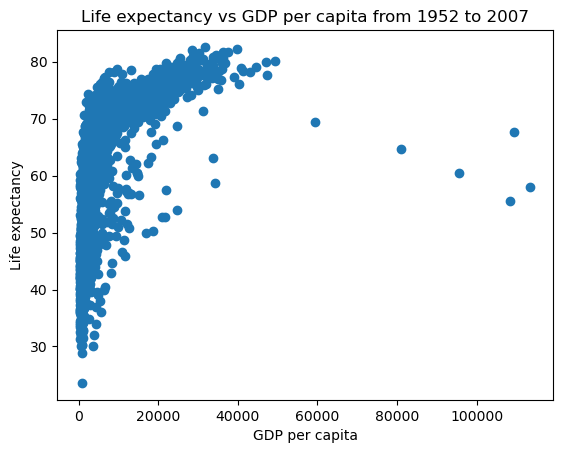
\includegraphics{Advanced_Data_Visualization_files/figure-pdf/cell-4-output-1.png}

}

\end{figure}

\begin{Shaded}
\begin{Highlighting}[]
\CommentTok{\#pyplot interface}
\NormalTok{x }\OperatorTok{=}\NormalTok{ gdp\_data.gdpPercap}
\NormalTok{y }\OperatorTok{=}\NormalTok{ gdp\_data.lifeExp}
\NormalTok{plt.plot(x,y,}\StringTok{\textquotesingle{}o\textquotesingle{}}\NormalTok{) }\CommentTok{\#By default, the plot() function makes a lineplot. The \textquotesingle{}o\textquotesingle{} arguments specifies a scatterplot}
\NormalTok{plt.xlabel(}\StringTok{\textquotesingle{}GDP per capita\textquotesingle{}}\NormalTok{)  }\CommentTok{\#Labelling the horizontal X{-}axis}
\NormalTok{plt.ylabel(}\StringTok{\textquotesingle{}Life expectancy\textquotesingle{}}\NormalTok{) }\CommentTok{\#Labelling the verical Y{-}axis}
\NormalTok{plt.title(}\StringTok{\textquotesingle{}Life expectancy vs GDP per capita from 1952 to 2007\textquotesingle{}}\NormalTok{)}\OperatorTok{;}
\end{Highlighting}
\end{Shaded}

\begin{figure}[H]

{\centering 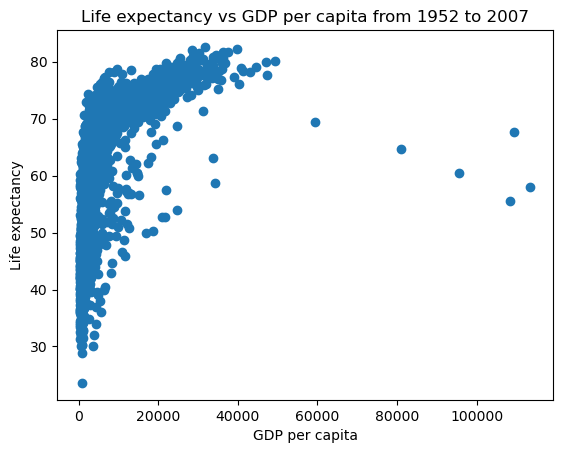
\includegraphics{Advanced_Data_Visualization_files/figure-pdf/cell-5-output-1.png}

}

\end{figure}

\hypertarget{pyplot-interface}{%
\subsection{Pyplot Interface}\label{pyplot-interface}}

In the previous chapter, our plotting is completely based on pyplot
interface of Matplotlib, which is just for basic plotting. You can
easily generate plots using pyplot module in the matplotlib library just
by importing \texttt{matplotlib.pyplot} module.

\begin{itemize}
\tightlist
\item
  pyplot interface is a \textbf{state-based interface.} It implicitly
  tracks the plot that it wants to reference
\item
  Simple functions are used to \textbf{add plot elements and/or modify
  the plot} as we need, whenever we need it.
\item
  The Pyplot interface \textbf{shares a lot of similarities in syntax
  and methodology with MATLAB.}
\end{itemize}

However, The \texttt{pyplot} interface has limited functionality in
these two cases:

\begin{itemize}
\tightlist
\item
  when there is a need to make multiple plots
\item
  when we have to make plots that require a lot of customization.
\end{itemize}

For more advanced plotting with Matplotlib, you have to learn
Object-Oriented Interface.

\hypertarget{plotting-with-object-oriented-interface-of-matplotlib}{%
\section{Plotting with Object-Oriented Interface of
Matplotlib}\label{plotting-with-object-oriented-interface-of-matplotlib}}

\hypertarget{understanding-matplotlib-object-hierarchy}{%
\subsection{Understanding Matplotlib Object
Hierarchy}\label{understanding-matplotlib-object-hierarchy}}

To understand the object-oriented interface of Matplotlib, we have to
start with a couple of fundamental concepts related to a plot. * Figure
* Axes

Think of the entire plot as an object hierarchy with Figure at the top
of it. Here is a small subset of the hierarchy with Figure being at the
top, followed by Axes ( not the same as axis ), followed by different
texts on the plot, different kinds of plots it can handle, the different
axis and so on. The hierarchy doesn't stop there. Further to x-axis for
example, there are ticks and further to ticks there are its subsequent
properties and so on.

\includegraphics{index_files/mediabag/matplotlib-object-or.png}

\hypertarget{figure}{%
\subsubsection{Figure}\label{figure}}

The outermost object is the figure which is an instance of
\texttt{figure.Figure}. It is the \textbf{top level container} for all
the plot elements. The Figure is the final image that may contain one or
more Axes and it keeps track of all the Axes. Figure is only a container
and you can not plot data on figure.

\begin{Shaded}
\begin{Highlighting}[]
\CommentTok{\# To begin with, we create a fiture instance which provides an empty canvas}
\NormalTok{fig }\OperatorTok{=}\NormalTok{ plt.figure()}
\end{Highlighting}
\end{Shaded}

\begin{verbatim}
<Figure size 640x480 with 0 Axes>
\end{verbatim}

Figure is just a container, note that creating figure using
\texttt{plt.figure()} does not automatically create an axes and hence
all you can see is the figure object.

\hypertarget{axes-1}{%
\subsubsection{Axes}\label{axes-1}}

\texttt{Axes} is the instance of \texttt{matplotlib.axes.Axes}. Axes
\textbf{is the area on which data are plotted}. A given figure can
contain many Axes, but a given Axes object can only be in one Figure.

\hypertarget{creating-an-axes-object-explicitly}{%
\paragraph{Creating an Axes Object
Explicitly}\label{creating-an-axes-object-explicitly}}

In the OOP interface, Axes objects are usually created using
\texttt{plt.subplots()} or \texttt{plt.figure().add\_subplot()}.

\begin{Shaded}
\begin{Highlighting}[]
\CommentTok{\# A figure only contains one axes by default}
\NormalTok{fig }\OperatorTok{=}\NormalTok{ plt.figure()}
\CommentTok{\# add axes to the figure}
\NormalTok{ax }\OperatorTok{=}\NormalTok{ fig.add\_subplot()}
\end{Highlighting}
\end{Shaded}

\begin{figure}[H]

{\centering 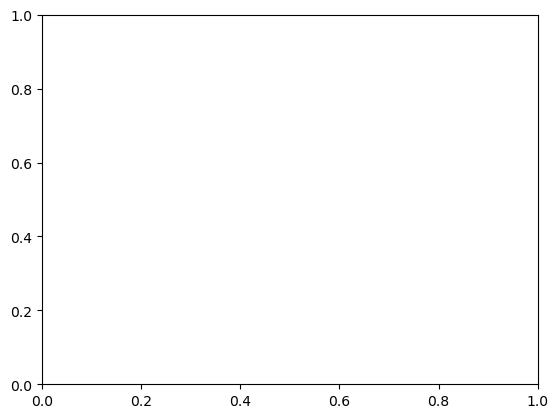
\includegraphics{Advanced_Data_Visualization_files/figure-pdf/cell-7-output-1.png}

}

\end{figure}

We create a blank axes (area) for plotting, if we need to add more axes
to the figure

\begin{Shaded}
\begin{Highlighting}[]
\CommentTok{\# create a figure with 4 axes, arranged in 2 rows and 2 columns}
\NormalTok{fig, axes }\OperatorTok{=}\NormalTok{ plt.subplots(}\DecValTok{2}\NormalTok{, }\DecValTok{2}\NormalTok{)}
\end{Highlighting}
\end{Shaded}

\begin{figure}[H]

{\centering 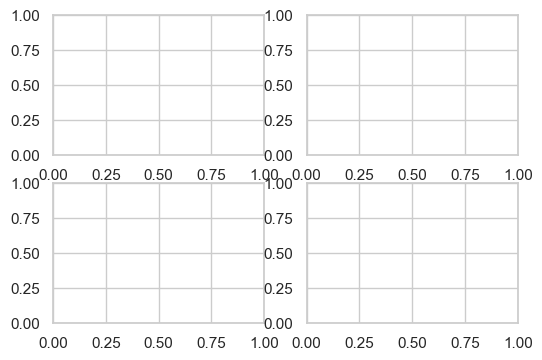
\includegraphics{Advanced_Data_Visualization_files/figure-pdf/cell-8-output-1.png}

}

\end{figure}

\hypertarget{components-of-an-axes-object}{%
\paragraph{Components of an Axes
Object}\label{components-of-an-axes-object}}

The \texttt{Axes} object contains several elements that make up the plot

\begin{itemize}
\tightlist
\item
  Data plotting area: Contains the data (lines, bars, points, etc.).
\item
  X-axis and Y-axis: Controls the axis limits, labels, and ticks.
\item
  Title and Labels: The overall title and labels for each axis.
\item
  Gridlines: Optional lines to help align the data visually.
\item
  Spines: The borders around the plot.
\item
  Legend: An optional component to explain the data series.
\item
  Annotations: Text or arrows highlighting points of interest.
\end{itemize}

This is what makes the \texttt{Axes} object central to any plot in the
OOP interface of Matplotlib.

\begin{Shaded}
\begin{Highlighting}[]
\CommentTok{\# create data for plotting}
\NormalTok{x }\OperatorTok{=}\NormalTok{ np.arange(}\DecValTok{10}\NormalTok{)}
\NormalTok{y }\OperatorTok{=}\NormalTok{ x}\OperatorTok{**}\DecValTok{2} 

\CommentTok{\# create a figure and axes}
\NormalTok{fig,ax }\OperatorTok{=}\NormalTok{ plt.subplots(}\DecValTok{1}\NormalTok{,}\DecValTok{1}\NormalTok{) }

\CommentTok{\# plot the data}
\NormalTok{ax.plot(x,y)}

\CommentTok{\# set the title}
\NormalTok{ax.set\_title(}\StringTok{"Exponential Plot"}\NormalTok{)}
 
\CommentTok{\# set the labels of x and y axes}
\NormalTok{ax.set\_xlabel(}\StringTok{"age"}\NormalTok{)}
\NormalTok{ax.set\_ylabel(}\StringTok{"Cell growth"}\NormalTok{)}

\CommentTok{\# set the limits of x and y axes}
\NormalTok{ax.set\_xlim([}\DecValTok{0}\NormalTok{, }\DecValTok{10}\NormalTok{])}
\NormalTok{ax.set\_ylim([}\DecValTok{0}\NormalTok{, }\DecValTok{100}\NormalTok{])}

\CommentTok{\# set the ticks of x and y axes}
\NormalTok{ax.set\_xticks(}\BuiltInTok{range}\NormalTok{(}\DecValTok{0}\NormalTok{, }\DecValTok{11}\NormalTok{, }\DecValTok{2}\NormalTok{))}
\NormalTok{ax.set\_yticks(}\BuiltInTok{range}\NormalTok{(}\DecValTok{0}\NormalTok{, }\DecValTok{101}\NormalTok{, }\DecValTok{20}\NormalTok{))}

\CommentTok{\# add grid}
\NormalTok{ax.grid(}\VariableTok{True}\NormalTok{)}

\CommentTok{\# add legend}
\NormalTok{ax.legend([}\StringTok{"y = x\^{}2"}\NormalTok{], loc }\OperatorTok{=} \StringTok{"upper left"}\NormalTok{)}

\CommentTok{\# show the plot}
\NormalTok{plt.show()}
\end{Highlighting}
\end{Shaded}

\begin{figure}[H]

{\centering \includegraphics{Advanced_Data_Visualization_files/figure-pdf/cell-9-output-1.png}

}

\end{figure}

\hypertarget{creating-complex-plots-with-multiple-subplots}{%
\subsection{Creating Complex Plots with Multiple
Subplots}\label{creating-complex-plots-with-multiple-subplots}}

To help illustrate subplots in matplotlib, we can cover two scenarios:

\begin{itemize}
\tightlist
\item
  subplots that don't overlap and
\item
  subplots inside other subplots
\end{itemize}

\hypertarget{plotting-non-overlapped-subplots}{%
\subsubsection{Plotting non-overlapped
subplots}\label{plotting-non-overlapped-subplots}}

This is the most common use case, where multiple plots are placed next
to each other in a grid, without overlap. The \texttt{plt.subplots()}
function allows for a clean layout where each plot is contained in its
own space. You can specify the number of rows and columns to create a
grid of subplots.

\begin{Shaded}
\begin{Highlighting}[]
\NormalTok{flowers\_df }\OperatorTok{=}\NormalTok{ sns.load\_dataset(}\StringTok{\textquotesingle{}iris\textquotesingle{}}\NormalTok{)}
\NormalTok{tips\_df }\OperatorTok{=}\NormalTok{ sns.load\_dataset(}\StringTok{\textquotesingle{}tips\textquotesingle{}}\NormalTok{)}
\NormalTok{flights\_df }\OperatorTok{=}\NormalTok{ sns.load\_dataset(}\StringTok{"flights"}\NormalTok{).pivot(index}\OperatorTok{=}\StringTok{"month"}\NormalTok{, columns}\OperatorTok{=}\StringTok{"year"}\NormalTok{, values}\OperatorTok{=}\StringTok{"passengers"}\NormalTok{)}


\NormalTok{fig, axes }\OperatorTok{=}\NormalTok{ plt.subplots(}\DecValTok{2}\NormalTok{, }\DecValTok{2}\NormalTok{, figsize}\OperatorTok{=}\NormalTok{(}\DecValTok{10}\NormalTok{, }\DecValTok{6}\NormalTok{))}

\CommentTok{\# Pass the axes into seaborn}
\NormalTok{axes[}\DecValTok{0}\NormalTok{,}\DecValTok{0}\NormalTok{].set\_title(}\StringTok{\textquotesingle{}Sepal Length vs. Sepal Width\textquotesingle{}}\NormalTok{)}
\NormalTok{sns.scatterplot(x}\OperatorTok{=}\NormalTok{flowers\_df.sepal\_length, }
\NormalTok{                y}\OperatorTok{=}\NormalTok{flowers\_df.sepal\_width, }
\NormalTok{                hue}\OperatorTok{=}\NormalTok{flowers\_df.species, }
\NormalTok{                s}\OperatorTok{=}\DecValTok{100}\NormalTok{, }
\NormalTok{                ax}\OperatorTok{=}\NormalTok{axes[}\DecValTok{0}\NormalTok{,}\DecValTok{0}\NormalTok{])}

\CommentTok{\# Use the axes for plotting}
\NormalTok{axes[}\DecValTok{0}\NormalTok{,}\DecValTok{1}\NormalTok{].set\_title(}\StringTok{\textquotesingle{}Distribution of Sepal Width\textquotesingle{}}\NormalTok{)}
\NormalTok{sns.histplot(flowers\_df.sepal\_width, ax}\OperatorTok{=}\NormalTok{axes[}\DecValTok{0}\NormalTok{,}\DecValTok{1}\NormalTok{])}
\NormalTok{axes[}\DecValTok{0}\NormalTok{,}\DecValTok{1}\NormalTok{].legend([}\StringTok{\textquotesingle{}Setosa\textquotesingle{}}\NormalTok{, }\StringTok{\textquotesingle{}Versicolor\textquotesingle{}}\NormalTok{, }\StringTok{\textquotesingle{}Virginica\textquotesingle{}}\NormalTok{])}

\CommentTok{\# Pass the axes into seaborn}
\NormalTok{axes[}\DecValTok{1}\NormalTok{,}\DecValTok{0}\NormalTok{].set\_title(}\StringTok{\textquotesingle{}Restaurant bills\textquotesingle{}}\NormalTok{)}
\NormalTok{sns.barplot(x}\OperatorTok{=}\StringTok{\textquotesingle{}day\textquotesingle{}}\NormalTok{, y}\OperatorTok{=}\StringTok{\textquotesingle{}total\_bill\textquotesingle{}}\NormalTok{, hue}\OperatorTok{=}\StringTok{\textquotesingle{}sex\textquotesingle{}}\NormalTok{, data}\OperatorTok{=}\NormalTok{tips\_df, ax}\OperatorTok{=}\NormalTok{axes[}\DecValTok{1}\NormalTok{,}\DecValTok{0}\NormalTok{])}

\CommentTok{\# Pass the axes into seaborn}
\NormalTok{axes[}\DecValTok{1}\NormalTok{,}\DecValTok{1}\NormalTok{].set\_title(}\StringTok{\textquotesingle{}Flight traffic\textquotesingle{}}\NormalTok{)}
\NormalTok{sns.heatmap(flights\_df, cmap}\OperatorTok{=}\StringTok{\textquotesingle{}Blues\textquotesingle{}}\NormalTok{, ax}\OperatorTok{=}\NormalTok{axes[}\DecValTok{1}\NormalTok{,}\DecValTok{1}\NormalTok{])}

\NormalTok{plt.tight\_layout(pad}\OperatorTok{=}\DecValTok{2}\NormalTok{)}
\end{Highlighting}
\end{Shaded}

\begin{figure}[H]

{\centering \includegraphics{Advanced_Data_Visualization_files/figure-pdf/cell-10-output-1.png}

}

\end{figure}

\begin{itemize}
\tightlist
\item
  The \texttt{plt.tight\_layout()} ensures the subplots do not overlap
  by adjusting the spacing automatically.
\item
  Seaborn and pandas are wrappers of Matplotlib. To create a
  Seaborn/pandas plot in a specific Matplotlib subplot, you pass the
  \texttt{ax} parameter to the its plotting function. This allows you to
  use their visualization capabilities while fully controlling the
  layout of the plot using Matplotlib's \texttt{plt.subplots()}
\end{itemize}

\hypertarget{plotting-nested-subplots-subplots-inside-other-subplots}{%
\subsubsection{Plotting Nested Subplots (Subplots Inside Other
Subplots)}\label{plotting-nested-subplots-subplots-inside-other-subplots}}

You can create a subplot inside another plot using \texttt{add\_axes()}
or \texttt{inset\_axes()} from matplotlib's \texttt{Axes} object. This
is useful for creating insets or focusing on a specific region within a
larger plot.

Syntax of \texttt{add\_axes()}

\texttt{ax\ =\ fig.add\_axes({[}left,\ bottom,\ width,\ height{]})}

where * left: The x-position (horizontal starting point) of the axes, as
a fraction of the figure width (0 to 1). * bottom: The y-position
(vertical starting point) of the axes, as a fraction of the figure
height (0 to 1). * width: The width of the axes, as a fraction of the
figure width (0 to 1). * height: The height of the axes, as a fraction
of the figure height (0 to 1).

Below is an example demonstrating the use of \texttt{add\_axes()}. You
can also explore the \texttt{inset\_axes()} method for creating inset
plots with more flexibility

\begin{Shaded}
\begin{Highlighting}[]
\CommentTok{\# create inset axes within the main plot axes  }

\NormalTok{np.random.seed(}\DecValTok{19680801}\NormalTok{)  }\CommentTok{\# Fixing random state for reproducibility.}

\CommentTok{\# create some data to use for the plot}
\NormalTok{dt }\OperatorTok{=} \FloatTok{0.001}
\NormalTok{t }\OperatorTok{=}\NormalTok{ np.arange(}\FloatTok{0.0}\NormalTok{, }\FloatTok{10.0}\NormalTok{, dt)}
\NormalTok{r }\OperatorTok{=}\NormalTok{ np.exp(}\OperatorTok{{-}}\NormalTok{t[:}\DecValTok{1000}\NormalTok{] }\OperatorTok{/} \FloatTok{0.05}\NormalTok{)  }\CommentTok{\# impulse response}
\NormalTok{x }\OperatorTok{=}\NormalTok{ np.random.randn(}\BuiltInTok{len}\NormalTok{(t))}
\NormalTok{s }\OperatorTok{=}\NormalTok{ np.convolve(x, r)[:}\BuiltInTok{len}\NormalTok{(x)] }\OperatorTok{*}\NormalTok{ dt  }\CommentTok{\# colored noise}

\NormalTok{fig, main\_ax }\OperatorTok{=}\NormalTok{ plt.subplots()}
\NormalTok{main\_ax.plot(t, s)}
\NormalTok{main\_ax.set\_xlim(}\DecValTok{0}\NormalTok{, }\DecValTok{1}\NormalTok{)}
\NormalTok{main\_ax.set\_ylim(}\FloatTok{1.1} \OperatorTok{*}\NormalTok{ np.}\BuiltInTok{min}\NormalTok{(s), }\DecValTok{2} \OperatorTok{*}\NormalTok{ np.}\BuiltInTok{max}\NormalTok{(s))}
\NormalTok{main\_ax.set\_xlabel(}\StringTok{\textquotesingle{}time (s)\textquotesingle{}}\NormalTok{)}
\NormalTok{main\_ax.set\_ylabel(}\StringTok{\textquotesingle{}current (nA)\textquotesingle{}}\NormalTok{)}
\NormalTok{main\_ax.set\_title(}\StringTok{\textquotesingle{}Gaussian colored noise\textquotesingle{}}\NormalTok{)}

\CommentTok{\# this is an inset axes over the main axes}
\NormalTok{right\_inset\_ax }\OperatorTok{=}\NormalTok{ fig.add\_axes([}\FloatTok{.65}\NormalTok{, }\FloatTok{.6}\NormalTok{, }\FloatTok{.2}\NormalTok{, }\FloatTok{.2}\NormalTok{], facecolor}\OperatorTok{=}\StringTok{\textquotesingle{}k\textquotesingle{}}\NormalTok{)}
\NormalTok{right\_inset\_ax.hist(s, }\DecValTok{400}\NormalTok{, density}\OperatorTok{=}\VariableTok{True}\NormalTok{)}
\NormalTok{right\_inset\_ax.}\BuiltInTok{set}\NormalTok{(title}\OperatorTok{=}\StringTok{\textquotesingle{}Probability\textquotesingle{}}\NormalTok{, xticks}\OperatorTok{=}\NormalTok{[], yticks}\OperatorTok{=}\NormalTok{[])}

\CommentTok{\# this is another inset axes over the main axes}
\NormalTok{left\_inset\_ax }\OperatorTok{=}\NormalTok{ fig.add\_axes([}\FloatTok{.2}\NormalTok{, }\FloatTok{.6}\NormalTok{, }\FloatTok{.2}\NormalTok{, }\FloatTok{.2}\NormalTok{], facecolor}\OperatorTok{=}\StringTok{\textquotesingle{}k\textquotesingle{}}\NormalTok{)}
\NormalTok{left\_inset\_ax.plot(t[:}\BuiltInTok{len}\NormalTok{(r)], r)}
\NormalTok{left\_inset\_ax.}\BuiltInTok{set}\NormalTok{(title}\OperatorTok{=}\StringTok{\textquotesingle{}Impulse response\textquotesingle{}}\NormalTok{, xlim}\OperatorTok{=}\NormalTok{(}\DecValTok{0}\NormalTok{, }\FloatTok{.2}\NormalTok{), xticks}\OperatorTok{=}\NormalTok{[], yticks}\OperatorTok{=}\NormalTok{[])}

\NormalTok{plt.show()}
\end{Highlighting}
\end{Shaded}

\begin{figure}[H]

{\centering \includegraphics{Advanced_Data_Visualization_files/figure-pdf/cell-11-output-1.png}

}

\end{figure}

\hypertarget{advanced-customization-with-matplotlibs-object-oriented-interface}{%
\subsection{Advanced Customization with Matplotlib's Object-Oriented
Interface}\label{advanced-customization-with-matplotlibs-object-oriented-interface}}

Below, we are reading the dataset of noise complaints of type Loud
music/Party received the police in New York City in 2016.

\begin{Shaded}
\begin{Highlighting}[]
\NormalTok{nyc\_party\_complaints }\OperatorTok{=}\NormalTok{ pd.read\_csv(}\StringTok{\textquotesingle{}datasets/party\_nyc.csv\textquotesingle{}}\NormalTok{)}
\NormalTok{nyc\_party\_complaints.head()}
\end{Highlighting}
\end{Shaded}

\begin{longtable}[]{@{}lllllllllll@{}}
\toprule\noalign{}
& Created Date & Closed Date & Location Type & Incident Zip & City &
Borough & Latitude & Longitude & Hour\_of\_the\_day &
Month\_of\_the\_year \\
\midrule\noalign{}
\endhead
\bottomrule\noalign{}
\endlastfoot
0 & 12/31/2015 0:01 & 12/31/2015 3:48 & Store/Commercial & 10034.0 & NEW
YORK & MANHATTAN & 40.866183 & -73.918930 & 0 & 12 \\
1 & 12/31/2015 0:02 & 12/31/2015 4:36 & Store/Commercial & 10040.0 & NEW
YORK & MANHATTAN & 40.859324 & -73.931237 & 0 & 12 \\
2 & 12/31/2015 0:03 & 12/31/2015 0:40 & Residential Building/House &
10026.0 & NEW YORK & MANHATTAN & 40.799415 & -73.953371 & 0 & 12 \\
3 & 12/31/2015 0:03 & 12/31/2015 1:53 & Residential Building/House &
11231.0 & BROOKLYN & BROOKLYN & 40.678285 & -73.994668 & 0 & 12 \\
4 & 12/31/2015 0:05 & 12/31/2015 3:49 & Residential Building/House &
10033.0 & NEW YORK & MANHATTAN & 40.850304 & -73.938516 & 0 & 12 \\
\end{longtable}

Below, we will begin with basic plotting, utilizing Matplotlib's
object-oriented interface to handle more complex tasks, such as setting
the major axis formatting. When it comes to advanced customization,
Matplotlib's object-oriented interface offers greater flexibility and
control compared to the pyplot interface.

\hypertarget{bar-plots-with-pandas}{%
\subsubsection{Bar plots with Pandas}\label{bar-plots-with-pandas}}

\textbf{Purpose of bar plots}: Barplots are used to visualize any
aggregate statistics of a continuous variable with respect to the
categories or levels of a categorical variable.

Bar plots can be made using the pandas \texttt{bar} function with the
DataFrame or Series, just like the line plots and scatterplots.

Let us visualise the locations from where the the complaints are coming.

\begin{Shaded}
\begin{Highlighting}[]
\NormalTok{ax }\OperatorTok{=}\NormalTok{ nyc\_party\_complaints[}\StringTok{\textquotesingle{}Location Type\textquotesingle{}}\NormalTok{].value\_counts().plot.bar(ylabel }\OperatorTok{=} \StringTok{\textquotesingle{}Number of complaints\textquotesingle{}}\NormalTok{)}
\NormalTok{ax.yaxis.set\_major\_formatter(}\StringTok{\textquotesingle{}\{x:,.0f\}\textquotesingle{}}\NormalTok{)}
\end{Highlighting}
\end{Shaded}

\begin{figure}[H]

{\centering \includegraphics{Advanced_Data_Visualization_files/figure-pdf/cell-13-output-1.png}

}

\end{figure}

In the above code, we use \texttt{ax.yaxis.set\_major\_formatter} to
format the y-axis labels in a currency style. From the above plot, we
observe that most of the complaints come from residential buildings and
houses, as one may expect.

For categorical variables, we can use the \texttt{.value\_counts()}
method to get the statistical frequency of each unique value.

\begin{Shaded}
\begin{Highlighting}[]
\NormalTok{nyc\_party\_complaints[}\StringTok{\textquotesingle{}Location Type\textquotesingle{}}\NormalTok{].value\_counts()}
\end{Highlighting}
\end{Shaded}

\begin{verbatim}
Location Type
Residential Building/House    146040
Street/Sidewalk                42353
Store/Commercial               17617
Club/Bar/Restaurant            15766
Park/Playground                 3036
House of Worship                 602
Name: count, dtype: int64
\end{verbatim}

Next, Let is visualize the time of the year when most complaints occur.

\begin{Shaded}
\begin{Highlighting}[]
\NormalTok{nyc\_party\_complaints[}\StringTok{\textquotesingle{}Month\_of\_the\_year\textquotesingle{}}\NormalTok{].value\_counts()}
\end{Highlighting}
\end{Shaded}

\begin{verbatim}
Month_of_the_year
6     25933
5     25192
9     25000
7     24502
8     20833
10    19332
4     17718
12    15730
11    14146
3     13880
1     12171
2     10977
Name: count, dtype: int64
\end{verbatim}

\begin{Shaded}
\begin{Highlighting}[]
\CommentTok{\#Using the pandas function bar() to create bar plot}
\NormalTok{ax }\OperatorTok{=}\NormalTok{ nyc\_party\_complaints[}\StringTok{\textquotesingle{}Month\_of\_the\_year\textquotesingle{}}\NormalTok{].value\_counts().sort\_index().plot.bar(ylabel }\OperatorTok{=} \StringTok{\textquotesingle{}Number of complaints\textquotesingle{}}\NormalTok{,}
\NormalTok{                                                                              xlabel }\OperatorTok{=} \StringTok{"Month"}\NormalTok{)}
\NormalTok{ax.yaxis.set\_major\_formatter(}\StringTok{\textquotesingle{}\{x:,.0f\}\textquotesingle{}}\NormalTok{)}
\end{Highlighting}
\end{Shaded}

\begin{figure}[H]

{\centering \includegraphics{Advanced_Data_Visualization_files/figure-pdf/cell-16-output-1.png}

}

\end{figure}

Try executing the code without \texttt{sort\_index()} to figure out the
purpose of using the function.

From the above plot, we observe that most of the complaints occur during
summer and early Fall.

Let us create a stacked bar chart that combines both the above plots
into a single plot. You may ignore the code used for re-shaping the data
until Chapter 10. The purpose here is to show the utility of the pandas
\texttt{bar()} function.

\begin{Shaded}
\begin{Highlighting}[]
\CommentTok{\#Reshaping the data to make it suitable for a stacked barplot {-} ignore this code until chapter 8}
\NormalTok{complaints\_location}\OperatorTok{=}\NormalTok{pd.crosstab(nyc\_party\_complaints.Month\_of\_the\_year, nyc\_party\_complaints[}\StringTok{\textquotesingle{}Location Type\textquotesingle{}}\NormalTok{])}
\NormalTok{complaints\_location.head()}
\end{Highlighting}
\end{Shaded}

\begin{longtable}[]{@{}lllllll@{}}
\toprule\noalign{}
Location Type & Club/Bar/Restaurant & House of Worship & Park/Playground
& Residential Building/House & Store/Commercial & Street/Sidewalk \\
Month\_of\_the\_year & & & & & & \\
\midrule\noalign{}
\endhead
\bottomrule\noalign{}
\endlastfoot
1 & 748 & 24 & 17 & 9393 & 1157 & 832 \\
2 & 570 & 29 & 16 & 8383 & 1197 & 782 \\
3 & 747 & 39 & 90 & 9689 & 1480 & 1835 \\
4 & 848 & 53 & 129 & 11984 & 1761 & 2943 \\
5 & 2091 & 72 & 322 & 15676 & 1941 & 5090 \\
\end{longtable}

\begin{Shaded}
\begin{Highlighting}[]
\CommentTok{\#Stacked bar plot showing number of complaints at different months of the year, and from different locations}
\NormalTok{ax }\OperatorTok{=}\NormalTok{ complaints\_location.plot.bar(stacked}\OperatorTok{=}\VariableTok{True}\NormalTok{,ylabel }\OperatorTok{=} \StringTok{\textquotesingle{}Number of complaints\textquotesingle{}}\NormalTok{,figsize}\OperatorTok{=}\NormalTok{(}\DecValTok{15}\NormalTok{, }\DecValTok{10}\NormalTok{), xlabel }\OperatorTok{=} \StringTok{\textquotesingle{}Month\textquotesingle{}}\NormalTok{)}
\NormalTok{ax.tick\_params(axis }\OperatorTok{=} \StringTok{\textquotesingle{}both\textquotesingle{}}\NormalTok{,labelsize}\OperatorTok{=}\DecValTok{15}\NormalTok{)}
\NormalTok{ax.yaxis.set\_major\_formatter(}\StringTok{\textquotesingle{}\{x:,.0f\}\textquotesingle{}}\NormalTok{)}
\end{Highlighting}
\end{Shaded}

\begin{figure}[H]

{\centering \includegraphics{Advanced_Data_Visualization_files/figure-pdf/cell-18-output-1.png}

}

\end{figure}

The above plots gives the insights about location and day of the year
simultaneously that were previously separately obtained by the
individual plots.

An alternative to stacked barplots are side-by-side barplots, as shown
below.

\begin{Shaded}
\begin{Highlighting}[]
\CommentTok{\#Side{-}by{-}side bar plot showing number of complaints at different months of the year, and from different locations}
\NormalTok{ax }\OperatorTok{=}\NormalTok{ complaints\_location.plot.bar(ylabel }\OperatorTok{=} \StringTok{\textquotesingle{}Number of complaints\textquotesingle{}}\NormalTok{,figsize}\OperatorTok{=}\NormalTok{(}\DecValTok{15}\NormalTok{, }\DecValTok{10}\NormalTok{), xlabel }\OperatorTok{=} \StringTok{\textquotesingle{}Month\textquotesingle{}}\NormalTok{)}
\NormalTok{ax.tick\_params(axis }\OperatorTok{=} \StringTok{\textquotesingle{}both\textquotesingle{}}\NormalTok{,labelsize}\OperatorTok{=}\DecValTok{15}\NormalTok{)}
\NormalTok{ax.yaxis.set\_major\_formatter(}\StringTok{\textquotesingle{}\{x:,.0f\}\textquotesingle{}}\NormalTok{)}
\end{Highlighting}
\end{Shaded}

\begin{figure}[H]

{\centering \includegraphics{Advanced_Data_Visualization_files/figure-pdf/cell-19-output-1.png}

}

\end{figure}

Question: In which scenarios should we use a stacked barplot instead of
a side-by-side barplot and vice-versa?

\hypertarget{bar-plots-with-confidence-intervals-with-seaborn}{%
\subsubsection{Bar plots with confidence intervals with
Seaborn}\label{bar-plots-with-confidence-intervals-with-seaborn}}

We'll group the data to obtain the total complaints for each
\emph{Location Type, Borough, Month\_of\_the\_year, and
Hour\_of\_the\_day}. Note that you'll learn grouping data in later
chapters, so you may ignore the next code block. The grouping is done to
shape the data in a suitable form for visualization.

\begin{Shaded}
\begin{Highlighting}[]
\CommentTok{\#Grouping the data to make it suitable for visualization using Seaborn. Ignore this code block until learn chapter 9.}
\NormalTok{nyc\_complaints\_grouped }\OperatorTok{=}\NormalTok{ nyc\_party\_complaints[[}\StringTok{\textquotesingle{}Location Type\textquotesingle{}}\NormalTok{,}\StringTok{\textquotesingle{}Borough\textquotesingle{}}\NormalTok{,}\StringTok{\textquotesingle{}Month\_of\_the\_year\textquotesingle{}}\NormalTok{,}\StringTok{\textquotesingle{}Latitude\textquotesingle{}}\NormalTok{,}\StringTok{\textquotesingle{}Hour\_of\_the\_day\textquotesingle{}}\NormalTok{]].groupby([}\StringTok{\textquotesingle{}Location Type\textquotesingle{}}\NormalTok{,}\StringTok{\textquotesingle{}Borough\textquotesingle{}}\NormalTok{,}\StringTok{\textquotesingle{}Month\_of\_the\_year\textquotesingle{}}\NormalTok{,}\StringTok{\textquotesingle{}Hour\_of\_the\_day\textquotesingle{}}\NormalTok{])[}\StringTok{\textquotesingle{}Latitude\textquotesingle{}}\NormalTok{].agg([(}\StringTok{\textquotesingle{}complaints\textquotesingle{}}\NormalTok{,}\StringTok{\textquotesingle{}count\textquotesingle{}}\NormalTok{)]).reset\_index()}
\NormalTok{nyc\_complaints\_grouped.head()}
\end{Highlighting}
\end{Shaded}

\begin{longtable}[]{@{}llllll@{}}
\toprule\noalign{}
& Location Type & Borough & Month\_of\_the\_year & Hour\_of\_the\_day &
complaints \\
\midrule\noalign{}
\endhead
\bottomrule\noalign{}
\endlastfoot
0 & Club/Bar/Restaurant & BRONX & 1 & 0 & 10 \\
1 & Club/Bar/Restaurant & BRONX & 1 & 1 & 10 \\
2 & Club/Bar/Restaurant & BRONX & 1 & 2 & 6 \\
3 & Club/Bar/Restaurant & BRONX & 1 & 3 & 6 \\
4 & Club/Bar/Restaurant & BRONX & 1 & 4 & 3 \\
\end{longtable}

Let us create a bar plot visualizing the average number of complaints
with the time of the day.

\begin{Shaded}
\begin{Highlighting}[]
\NormalTok{ax }\OperatorTok{=}\NormalTok{ sns.barplot(x}\OperatorTok{=}\StringTok{"Hour\_of\_the\_day"}\NormalTok{, y }\OperatorTok{=} \StringTok{\textquotesingle{}complaints\textquotesingle{}}\NormalTok{,  data}\OperatorTok{=}\NormalTok{nyc\_complaints\_grouped)}
\NormalTok{ax.figure.set\_figwidth(}\DecValTok{15}\NormalTok{)}
\end{Highlighting}
\end{Shaded}

\begin{figure}[H]

{\centering \includegraphics{Advanced_Data_Visualization_files/figure-pdf/cell-21-output-1.png}

}

\end{figure}

From the above plot, we observe that most of the complaints are made
around midnight. However, interestingly, there are some complaints at
each hour of the day.

Note that the above barplot shows the mean number of complaints in a
month at each hour of the day. The black lines are the 95\% confidence
intervals of the mean number of complaints.

\hypertarget{pyplot-a-convenience-wrapper-around-the-object-oriented-interface}{%
\subsection{\texorpdfstring{\texttt{pyplot}: a convenience wrapper
around the object-oriented
interface}{pyplot: a convenience wrapper around the object-oriented interface}}\label{pyplot-a-convenience-wrapper-around-the-object-oriented-interface}}

While the pyplot interface is simpler for quick, basic plots, it
ultimately wraps around the object-oriented structure of Matplotlib,
meaning that it's built on top of the object-oriented interface.

\includegraphics{index_files/mediabag/title_xlabel_ylabel_.png}

\hypertarget{creating-subplots-with-seaborn}{%
\section{Creating Subplots with
Seaborn}\label{creating-subplots-with-seaborn}}

We previously demonstrated how Seaborn integrates seamlessly with
Matplotlib's object-oriented interface, allowing you to pass the
\texttt{ax} argument to any Seaborn function, thereby directing the plot
to a specific axis within a subplot grid.

Additionally, Seaborn offers a more convenient and simplified approach
to creating subplots, thanks to its high-level functions and built-in
integration with Matplotlib. Here's how Seaborn makes working with
subplots easier:

\hypertarget{using-facetgrid}{%
\subsection{\texorpdfstring{Using
\texttt{Facetgrid}}{Using Facetgrid}}\label{using-facetgrid}}

Seaborn's \texttt{FacetGrid} function make it very easy to create facet
grids or subplots based on data dimensions (such as categories), which
would require more manual effort with Matplotlib.

You can use the \texttt{row} and \texttt{col} parameters to control how
the data is split into subplots along these dimensions.

\begin{Shaded}
\begin{Highlighting}[]
\CommentTok{\# Seaborn Example using FacetGrid:}
\NormalTok{tips\_df }\OperatorTok{=}\NormalTok{ sns.load\_dataset(}\StringTok{"tips"}\NormalTok{)}
\NormalTok{tips\_df.head()}
\end{Highlighting}
\end{Shaded}

\begin{longtable}[]{@{}llllllll@{}}
\toprule\noalign{}
& total\_bill & tip & sex & smoker & day & time & size \\
\midrule\noalign{}
\endhead
\bottomrule\noalign{}
\endlastfoot
0 & 16.99 & 1.01 & Female & No & Sun & Dinner & 2 \\
1 & 10.34 & 1.66 & Male & No & Sun & Dinner & 3 \\
2 & 21.01 & 3.50 & Male & No & Sun & Dinner & 3 \\
3 & 23.68 & 3.31 & Male & No & Sun & Dinner & 2 \\
4 & 24.59 & 3.61 & Female & No & Sun & Dinner & 4 \\
\end{longtable}

\begin{Shaded}
\begin{Highlighting}[]
\NormalTok{g }\OperatorTok{=}\NormalTok{ sns.FacetGrid(tips\_df, col}\OperatorTok{=}\StringTok{\textquotesingle{}time\textquotesingle{}}\NormalTok{, row}\OperatorTok{=}\StringTok{\textquotesingle{}smoker\textquotesingle{}}\NormalTok{)}
\NormalTok{g.}\BuiltInTok{map}\NormalTok{(sns.histplot, }\StringTok{\textquotesingle{}total\_bill\textquotesingle{}}\NormalTok{, color}\OperatorTok{=}\StringTok{\textquotesingle{}r\textquotesingle{}}\NormalTok{)}
\NormalTok{g.set\_titles(col\_template}\OperatorTok{=}\StringTok{"}\SpecialCharTok{\{col\_name\}}\StringTok{"}\NormalTok{, row\_template}\OperatorTok{=}\StringTok{"Smoker: }\SpecialCharTok{\{row\_name\}}\StringTok{"}\NormalTok{)}\OperatorTok{;}
\end{Highlighting}
\end{Shaded}

\begin{figure}[H]

{\centering \includegraphics{Advanced_Data_Visualization_files/figure-pdf/cell-23-output-1.png}

}

\end{figure}

\begin{Shaded}
\begin{Highlighting}[]
\CommentTok{\# adding hue to the FacetGrid}
\NormalTok{g }\OperatorTok{=}\NormalTok{ sns.FacetGrid(tips\_df, col}\OperatorTok{=}\StringTok{\textquotesingle{}time\textquotesingle{}}\NormalTok{, row}\OperatorTok{=}\StringTok{\textquotesingle{}smoker\textquotesingle{}}\NormalTok{,hue}\OperatorTok{=}\StringTok{\textquotesingle{}size\textquotesingle{}}\NormalTok{)}
\CommentTok{\# Plot a scatterplot of the total bill and tip for each combination of time and smoker}
\NormalTok{g.}\BuiltInTok{map}\NormalTok{(sns.scatterplot, }\StringTok{\textquotesingle{}total\_bill\textquotesingle{}}\NormalTok{, }\StringTok{\textquotesingle{}tip\textquotesingle{}}\NormalTok{)}
\NormalTok{g.set\_titles(col\_template}\OperatorTok{=}\StringTok{"}\SpecialCharTok{\{col\_name\}}\StringTok{"}\NormalTok{, row\_template}\OperatorTok{=}\StringTok{"Smoker: }\SpecialCharTok{\{row\_name\}}\StringTok{"}\NormalTok{)}\OperatorTok{;}
\end{Highlighting}
\end{Shaded}

\begin{figure}[H]

{\centering \includegraphics{Advanced_Data_Visualization_files/figure-pdf/cell-24-output-1.png}

}

\end{figure}

\begin{Shaded}
\begin{Highlighting}[]
\CommentTok{\#Visualizing the number of complaints with Month\_of\_the\_year, Location Type, and Borough.}
\NormalTok{a }\OperatorTok{=}\NormalTok{ sns.FacetGrid(nyc\_complaints\_grouped, hue }\OperatorTok{=} \StringTok{\textquotesingle{}Location Type\textquotesingle{}}\NormalTok{, col }\OperatorTok{=} \StringTok{\textquotesingle{}Borough\textquotesingle{}}\NormalTok{,col\_wrap}\OperatorTok{=}\DecValTok{3}\NormalTok{,height}\OperatorTok{=}\FloatTok{3.5}\NormalTok{,aspect }\OperatorTok{=} \DecValTok{1}\NormalTok{)}
\CommentTok{\# Plotting a lineplot to show the number of complaints with Month\_of\_the\_year}
\NormalTok{a.}\BuiltInTok{map}\NormalTok{(sns.lineplot,}\StringTok{\textquotesingle{}Month\_of\_the\_year\textquotesingle{}}\NormalTok{,}\StringTok{\textquotesingle{}complaints\textquotesingle{}}\NormalTok{)}
\NormalTok{a.set\_axis\_labels(}\StringTok{"Month of the year"}\NormalTok{, }\StringTok{"Complaints"}\NormalTok{)}
\NormalTok{a.add\_legend()}
\end{Highlighting}
\end{Shaded}

\begin{figure}[H]

{\centering \includegraphics{Advanced_Data_Visualization_files/figure-pdf/cell-25-output-1.png}

}

\end{figure}

\hypertarget{using-pairplot}{%
\subsection{\texorpdfstring{Using
\texttt{Pairplot}}{Using Pairplot}}\label{using-pairplot}}

Pairplots are used to visualize the association between all
variable-pairs in the data. In other words, pairplots simultaneously
visualize the scatterplots between all variable-pairs.

Let us visualize the pair-wise association of tips variables in the tips
dataset

\begin{Shaded}
\begin{Highlighting}[]
\NormalTok{sns.pairplot(tips\_df )}\OperatorTok{;}
\end{Highlighting}
\end{Shaded}

\begin{figure}[H]

{\centering \includegraphics{Advanced_Data_Visualization_files/figure-pdf/cell-26-output-1.png}

}

\end{figure}

Let us visualize the pair-wise association of nutrition variables in the
starbucks drinks data.

\begin{Shaded}
\begin{Highlighting}[]
\NormalTok{starbucks\_drinks }\OperatorTok{=}\NormalTok{ pd.read\_csv(}\StringTok{\textquotesingle{}datasets/starbucks{-}menu{-}nutrition{-}drinks.csv\textquotesingle{}}\NormalTok{)}
\NormalTok{sns.pairplot(starbucks\_drinks)}\OperatorTok{;}
\end{Highlighting}
\end{Shaded}

\begin{figure}[H]

{\centering \includegraphics{Advanced_Data_Visualization_files/figure-pdf/cell-27-output-1.png}

}

\end{figure}

In the above pairplot, note that:

\begin{itemize}
\tightlist
\item
  The histograms on the diagonal of the grid show the distribution of
  each of the variables.
\item
  Instead of a histogram, we can visualize the density plot with the
  argument kde = True.
\item
  The scatterplots in the rest of the grid are the pair-wise plots of
  all the variables.
\end{itemize}

\hypertarget{geosptial-plotting}{%
\section{Geosptial Plotting}\label{geosptial-plotting}}

There are several widely used Python packages pecifically designed for
working with geospatial datasets. In this lesson, we will cover:

\begin{itemize}
\tightlist
\item
  GeoPandas
\item
  Folium
\end{itemize}

Let's import them

\begin{Shaded}
\begin{Highlighting}[]
\ImportTok{import}\NormalTok{ geopandas }\ImportTok{as}\NormalTok{ gpd}
\ImportTok{import}\NormalTok{ geopandas }
\ImportTok{import}\NormalTok{ folium}
\ImportTok{import}\NormalTok{ geodatasets}
\end{Highlighting}
\end{Shaded}

\hypertarget{static-plots-with-geopandas}{%
\subsection{Static Plots with
GeoPandas}\label{static-plots-with-geopandas}}

\begin{Shaded}
\begin{Highlighting}[]
\CommentTok{\# Create figure and axis}
\NormalTok{fig, ax }\OperatorTok{=}\NormalTok{ plt.subplots(figsize}\OperatorTok{=}\NormalTok{(}\DecValTok{15}\NormalTok{, }\DecValTok{10}\NormalTok{))}

\CommentTok{\# Plot your GeoDataFrame}
\NormalTok{chicago }\OperatorTok{=}\NormalTok{ gpd.read\_file(}\StringTok{\textquotesingle{}datasets/chicago\_boundaries\textbackslash{}geo\_export\_26bce2f2{-}c163{-}42a9{-}9329{-}9ca6e082c5e9.shp\textquotesingle{}}\NormalTok{)}
\NormalTok{chicago.plot(column}\OperatorTok{=}\StringTok{\textquotesingle{}community\textquotesingle{}}\NormalTok{, ax}\OperatorTok{=}\NormalTok{ax, legend}\OperatorTok{=}\VariableTok{True}\NormalTok{, legend\_kwds}\OperatorTok{=}\NormalTok{\{}\StringTok{\textquotesingle{}ncol\textquotesingle{}}\NormalTok{: }\DecValTok{2}\NormalTok{, }\StringTok{\textquotesingle{}bbox\_to\_anchor\textquotesingle{}}\NormalTok{: (}\DecValTok{2}\NormalTok{, }\DecValTok{1}\NormalTok{)\})}

\CommentTok{\# Add title (optional)}
\NormalTok{plt.title(}\StringTok{\textquotesingle{}Chicago Community Areas\textquotesingle{}}\NormalTok{)}

\CommentTok{\# Show the plot}
\NormalTok{plt.show()}\OperatorTok{;}
\end{Highlighting}
\end{Shaded}

\begin{verbatim}
<>:5: SyntaxWarning: invalid escape sequence '\g'
<>:5: SyntaxWarning: invalid escape sequence '\g'
C:\Users\lsi8012\AppData\Local\Temp\ipykernel_14232\2125888739.py:5: SyntaxWarning: invalid escape sequence '\g'
  chicago = gpd.read_file('datasets/chicago_boundaries\geo_export_26bce2f2-c163-42a9-9329-9ca6e082c5e9.shp')
\end{verbatim}

\begin{figure}[H]

{\centering \includegraphics{Advanced_Data_Visualization_files/figure-pdf/cell-29-output-2.png}

}

\end{figure}

\hypertarget{dataset-bicycle-sharing-in-chicago}{%
\subsection{Dataset: Bicycle Sharing in
Chicago}\label{dataset-bicycle-sharing-in-chicago}}

Divvy is Chicagoland's bike share system (in collaboration with Chicago
Department of Transportation), with 6,000 bikes available at 570+
stations across Chicago and Evanston. Divvy provides residents and
visitors with a convenient, fun and affordable transportation option for
getting around and exploring Chicago.

Divvy, like other bike share systems, consists of a fleet of specially
designed, sturdy and durable bikes that are locked into a network of
docking stations throughout the region. The bikes can be unlocked from
one station and returned to any other station in the system. People use
bike share to explore Chicago, commute to work or school, run errands,
get to appointments or social engagements, and more.

Divvy is available for use 24 hours/day, 7 days/week, 365 days/year, and
riders have access to all bikes and stations across the system.

We will be using divvy trips in the year of 2013

\begin{Shaded}
\begin{Highlighting}[]
\CommentTok{\# read the csv file\textquotesingle{}divvy\_2013.csv\textquotesingle{} into pandas pandas dataframe}
\NormalTok{data }\OperatorTok{=}\NormalTok{ pd.read\_csv(}\StringTok{\textquotesingle{}datasets/divvy\_2013.csv\textquotesingle{}}\NormalTok{)}
\NormalTok{data.head()}
\end{Highlighting}
\end{Shaded}

\begin{longtable}[]{@{}llllllllllllllllllllll@{}}
\toprule\noalign{}
& trip\_id & usertype & gender & starttime & stoptime & tripduration &
from\_station\_id & from\_station\_name & latitude\_start &
longitude\_start & ... & dewpoint & humidity & pressure & visibility &
wind\_speed & precipitation & events & rain & conditions & month \\
\midrule\noalign{}
\endhead
\bottomrule\noalign{}
\endlastfoot
0 & 3940 & Subscriber & Male & 2013-06-27 01:06:00 & 2013-06-27 09:46:00
& 31177 & 91 & Clinton St \& Washington Blvd & 41.88338 & -87.641170 &
... & 64.9 & 96.0 & 29.75 & 7.0 & 0.0 & -9999.0 & partlycloudy & 0 &
Scattered Clouds & 6 \\
1 & 4095 & Subscriber & Male & 2013-06-27 12:06:00 & 2013-06-27 12:11:00
& 301 & 85 & Michigan Ave \& Oak St & 41.90096 & -87.623777 & ... & 69.1
& 55.0 & 29.75 & 10.0 & 13.8 & -9999.0 & mostlycloudy & 0 & Mostly
Cloudy & 6 \\
2 & 4113 & Subscriber & Male & 2013-06-27 11:09:00 & 2013-06-27 11:11:00
& 140 & 88 & May St \& Randolph St & 41.88397 & -87.655688 & ... & 70.0
& 61.0 & 29.75 & 10.0 & 10.4 & -9999.0 & mostlycloudy & 0 & Mostly
Cloudy & 6 \\
3 & 4118 & Customer & NaN & 2013-06-27 12:11:00 & 2013-06-27 12:16:00 &
316 & 85 & Michigan Ave \& Oak St & 41.90096 & -87.623777 & ... & 69.1 &
55.0 & 29.75 & 10.0 & 13.8 & -9999.0 & mostlycloudy & 0 & Mostly Cloudy
& 6 \\
4 & 4119 & Subscriber & Male & 2013-06-27 11:12:00 & 2013-06-27 11:13:00
& 87 & 88 & May St \& Randolph St & 41.88397 & -87.655688 & ... & 70.0 &
61.0 & 29.75 & 10.0 & 10.4 & -9999.0 & mostlycloudy & 0 & Mostly Cloudy
& 6 \\
\end{longtable}

Below are basic data cleaning

\begin{Shaded}
\begin{Highlighting}[]
\CommentTok{\# drop the duplicates in the column \textquotesingle{}to\_station\_id\textquotesingle{}, \textquotesingle{}to\_station\_name\textquotesingle{}, \textquotesingle{}latitude\_end\textquotesingle{}, \textquotesingle{}longitude\_end\textquotesingle{}}
\NormalTok{data\_station\_same }\OperatorTok{=}\NormalTok{ data[[}\StringTok{\textquotesingle{}from\_station\_id\textquotesingle{}}\NormalTok{, }\StringTok{\textquotesingle{}from\_station\_name\textquotesingle{}}\NormalTok{, }\StringTok{\textquotesingle{}latitude\_start\textquotesingle{}}\NormalTok{, }\StringTok{\textquotesingle{}longitude\_start\textquotesingle{}}\NormalTok{, }\StringTok{\textquotesingle{}to\_station\_id\textquotesingle{}}\NormalTok{, }\StringTok{\textquotesingle{}to\_station\_name\textquotesingle{}}\NormalTok{, }\StringTok{\textquotesingle{}latitude\_end\textquotesingle{}}\NormalTok{, }\StringTok{\textquotesingle{}longitude\_end\textquotesingle{}}\NormalTok{]].drop\_duplicates()}
\NormalTok{data\_station\_same.shape}
\end{Highlighting}
\end{Shaded}

\begin{verbatim}
(1757, 8)
\end{verbatim}

\hypertarget{adding-the-divvy-station-to-the-plot}{%
\subsection{Adding the divvy station to the
plot}\label{adding-the-divvy-station-to-the-plot}}

\begin{Shaded}
\begin{Highlighting}[]
\CommentTok{\# Adding the stations to the plot}
\NormalTok{fig, ax }\OperatorTok{=}\NormalTok{ plt.subplots(figsize}\OperatorTok{=}\NormalTok{(}\DecValTok{15}\NormalTok{, }\DecValTok{10}\NormalTok{))}

\NormalTok{chicago }\OperatorTok{=}\NormalTok{ gpd.read\_file(}\StringTok{\textquotesingle{}datasets/chicago\_boundaries\textbackslash{}geo\_export\_26bce2f2{-}c163{-}42a9{-}9329{-}9ca6e082c5e9.shp\textquotesingle{}}\NormalTok{)}
\NormalTok{chicago.plot(column}\OperatorTok{=}\StringTok{\textquotesingle{}community\textquotesingle{}}\NormalTok{, ax}\OperatorTok{=}\NormalTok{ax, legend}\OperatorTok{=}\VariableTok{True}\NormalTok{, legend\_kwds}\OperatorTok{=}\NormalTok{\{}\StringTok{\textquotesingle{}ncol\textquotesingle{}}\NormalTok{: }\DecValTok{2}\NormalTok{, }\StringTok{\textquotesingle{}bbox\_to\_anchor\textquotesingle{}}\NormalTok{: (}\DecValTok{2}\NormalTok{, }\DecValTok{1}\NormalTok{)\})}

\CommentTok{\# Plot the stations}
\NormalTok{longlat\_df }\OperatorTok{=}\NormalTok{ data[[ }\StringTok{\textquotesingle{}latitude\_start\textquotesingle{}}\NormalTok{, }\StringTok{\textquotesingle{}longitude\_start\textquotesingle{}}\NormalTok{]].drop\_duplicates()}

\NormalTok{plt.scatter(longlat\_df[}\StringTok{\textquotesingle{}longitude\_start\textquotesingle{}}\NormalTok{], longlat\_df[}\StringTok{\textquotesingle{}latitude\_start\textquotesingle{}}\NormalTok{], s}\OperatorTok{=}\DecValTok{10}\NormalTok{, alpha}\OperatorTok{=}\FloatTok{0.5}\NormalTok{, color}\OperatorTok{=}\StringTok{\textquotesingle{}black\textquotesingle{}}\NormalTok{, marker}\OperatorTok{=}\StringTok{\textquotesingle{}o\textquotesingle{}}\NormalTok{)}
\CommentTok{\# data[[\textquotesingle{}longitude\_start\textquotesingle{}, \textquotesingle{}latitude\_start\textquotesingle{}]].drop\_duplicates().plot(ax=ax, color=\textquotesingle{}red\textquotesingle{}, markersize=10, marker=\textquotesingle{}o\textquotesingle{})}

\CommentTok{\# Add title (optional)}
\NormalTok{plt.title(}\StringTok{\textquotesingle{}Chicago Community Areas\textquotesingle{}}\NormalTok{)}

\CommentTok{\# Show the plot}
\NormalTok{plt.show()}
\end{Highlighting}
\end{Shaded}

\begin{verbatim}
<>:4: SyntaxWarning: invalid escape sequence '\g'
<>:4: SyntaxWarning: invalid escape sequence '\g'
C:\Users\lsi8012\AppData\Local\Temp\ipykernel_14232\1459074587.py:4: SyntaxWarning: invalid escape sequence '\g'
  chicago = gpd.read_file('datasets/chicago_boundaries\geo_export_26bce2f2-c163-42a9-9329-9ca6e082c5e9.shp')
\end{verbatim}

\begin{figure}[H]

{\centering \includegraphics{Advanced_Data_Visualization_files/figure-pdf/cell-32-output-2.png}

}

\end{figure}

\hypertarget{change-the-chicago-shapefile}{%
\subsection{Change the chicago
shapefile}\label{change-the-chicago-shapefile}}

\begin{Shaded}
\begin{Highlighting}[]
\NormalTok{chicago }\OperatorTok{=}\NormalTok{ gpd.read\_file(geodatasets.get\_path(}\StringTok{"geoda.chicago\_commpop"}\NormalTok{))}

\CommentTok{\# Plot the data}
\NormalTok{fig, ax }\OperatorTok{=}\NormalTok{ plt.subplots(figsize}\OperatorTok{=}\NormalTok{(}\DecValTok{15}\NormalTok{, }\DecValTok{10}\NormalTok{))}
\NormalTok{chicago.boundary.plot(ax}\OperatorTok{=}\NormalTok{ax)}
\NormalTok{plt.scatter(data[}\StringTok{\textquotesingle{}longitude\_start\textquotesingle{}}\NormalTok{], data[}\StringTok{\textquotesingle{}latitude\_start\textquotesingle{}}\NormalTok{], s}\OperatorTok{=}\DecValTok{10}\NormalTok{, alpha}\OperatorTok{=}\FloatTok{0.5}\NormalTok{, color}\OperatorTok{=}\StringTok{\textquotesingle{}black\textquotesingle{}}\NormalTok{, marker}\OperatorTok{=}\StringTok{\textquotesingle{}o\textquotesingle{}}\NormalTok{)}
\NormalTok{plt.title(}\StringTok{\textquotesingle{}Chicago Community Areas\textquotesingle{}}\NormalTok{)}
\end{Highlighting}
\end{Shaded}

\begin{verbatim}
Text(0.5, 1.0, 'Chicago Community Areas')
\end{verbatim}

\begin{figure}[H]

{\centering \includegraphics{Advanced_Data_Visualization_files/figure-pdf/cell-33-output-2.png}

}

\end{figure}

\hypertarget{interactive-plotting}{%
\subsection{Interactive Plotting}\label{interactive-plotting}}

Alongside static plots, \texttt{geopandas} can create interactive maps
based on the
\href{https://python-visualization.github.io/folium/latest/}{folium}
library.

Creating maps for interactive exploration mirrors the API of static
\href{https://geopandas.org/en/stable/docs/reference/api/geopandas.GeoDataFrame.plot.html}{plots}
in an
\href{https://geopandas.org/en/stable/docs/reference/api/geopandas.GeoDataFrame.explore.html}{explore()}
method of a GeoSeries or GeoDataFrame.

Here's an explanation of how \texttt{explore()} works and its key
features:

Key Features of \texttt{explore()}:

\begin{enumerate}
\def\labelenumi{\arabic{enumi}.}
\tightlist
\item
  Interactive Map Display:
\end{enumerate}

\begin{itemize}
\tightlist
\item
  When you call explore() on a Geodataframe (gdf), it launches an
  interactive map widget directly within your Jupyter notebook.
\item
  This map allows you to pan, zoom, and interact with the geometries
  (points, lines, polygons) in your Geodataframe.
\end{itemize}

\begin{enumerate}
\def\labelenumi{\arabic{enumi}.}
\setcounter{enumi}{1}
\tightlist
\item
  Layer Control:
\end{enumerate}

\begin{itemize}
\tightlist
\item
  explore() automatically adds the geometries from your Geodataframe as
  layers on the map.
\item
  Each geometry type (points, lines, polygons) is displayed with
  appropriate styling and markers.
\end{itemize}

\begin{enumerate}
\def\labelenumi{\arabic{enumi}.}
\setcounter{enumi}{2}
\tightlist
\item
  Tooltip Information:
\end{enumerate}

\begin{itemize}
\tightlist
\item
  When you hover over a geometry in the map, explore() displays tooltip
  information that typically includes attribute data associated with
  that geometry.
\item
  This feature is useful for inspecting specific details or properties
  of individual features in your geospatial dataset.
\end{itemize}

\begin{enumerate}
\def\labelenumi{\arabic{enumi}.}
\setcounter{enumi}{3}
\tightlist
\item
  Search and Filter:
\end{enumerate}

\begin{itemize}
\tightlist
\item
  explore() provides basic search and filter functionalities directly on
  the map.
\item
  You can search for specific attribute values or filter the displayed
  features based on attribute criteria defined in your Geodataframe.
\end{itemize}

\begin{enumerate}
\def\labelenumi{\arabic{enumi}.}
\setcounter{enumi}{4}
\tightlist
\item
  Customization:
\end{enumerate}

\begin{itemize}
\tightlist
\item
  Although explore() provides default styling and interaction behaviors,
  you can customize the map further using parameters or by manipulating
  the Geodataframe before calling explore().
\end{itemize}

\begin{Shaded}
\begin{Highlighting}[]
\CommentTok{\# use the geopandas explore default settings}
\NormalTok{chicago }\OperatorTok{=}\NormalTok{ gpd.read\_file(geodatasets.get\_path(}\StringTok{"geoda.chicago\_commpop"}\NormalTok{))}

\NormalTok{chicago.explore()}
\end{Highlighting}
\end{Shaded}

\begin{verbatim}
<folium.folium.Map at 0x1f6a6f672c0>
\end{verbatim}

Adding the population layer

\begin{Shaded}
\begin{Highlighting}[]
\CommentTok{\# Customerize the explore settings}
\NormalTok{chicago }\OperatorTok{=}\NormalTok{ gpd.read\_file(geodatasets.get\_path(}\StringTok{"geoda.chicago\_commpop"}\NormalTok{))}

\NormalTok{m }\OperatorTok{=}\NormalTok{ chicago.explore(}
\NormalTok{    column}\OperatorTok{=}\StringTok{"POP2010"}\NormalTok{,  }\CommentTok{\# make choropleth based on "POP2010" column}
\NormalTok{    scheme}\OperatorTok{=}\StringTok{"naturalbreaks"}\NormalTok{,  }\CommentTok{\# use mapclassify\textquotesingle{}s natural breaks scheme}
\NormalTok{    legend}\OperatorTok{=}\VariableTok{True}\NormalTok{,  }\CommentTok{\# show legend}
\NormalTok{    k}\OperatorTok{=}\DecValTok{10}\NormalTok{,  }\CommentTok{\# use 10 bins}
\NormalTok{    tooltip}\OperatorTok{=}\VariableTok{False}\NormalTok{,  }\CommentTok{\# hide tooltip}
\NormalTok{    popup}\OperatorTok{=}\NormalTok{[}\StringTok{"POP2010"}\NormalTok{, }\StringTok{"POP2000"}\NormalTok{],  }\CommentTok{\# show popup (on{-}click)}
\NormalTok{    legend\_kwds}\OperatorTok{=}\BuiltInTok{dict}\NormalTok{(colorbar}\OperatorTok{=}\VariableTok{False}\NormalTok{),  }\CommentTok{\# do not use colorbar}
\NormalTok{    name}\OperatorTok{=}\StringTok{"chicago"}\NormalTok{,  }\CommentTok{\# name of the layer in the map}
\NormalTok{)}

\NormalTok{m}
\end{Highlighting}
\end{Shaded}

\begin{verbatim}
c:\Users\lsi8012\AppData\Local\anaconda3\Lib\site-packages\sklearn\cluster\_kmeans.py:1446: UserWarning: KMeans is known to have a memory leak on Windows with MKL, when there are less chunks than available threads. You can avoid it by setting the environment variable OMP_NUM_THREADS=1.
  warnings.warn(
\end{verbatim}

\begin{verbatim}
<folium.folium.Map at 0x1f6a7436e40>
\end{verbatim}

The \texttt{explore()} method returns a \texttt{folium.Map} object,
which can also be passed directly (as you do with \texttt{ax} in
\texttt{plot()}). You can then use folium functionality directly on the
resulting map. Next, let's add the divvy station plot.

\begin{Shaded}
\begin{Highlighting}[]
\BuiltInTok{type}\NormalTok{(m)}
\end{Highlighting}
\end{Shaded}

\begin{verbatim}
folium.folium.Map
\end{verbatim}

\hypertarget{adding-the-divvy-station-on-the-interactive-folium.map}{%
\subsection{\texorpdfstring{Adding the divvy station on the interactive
\texttt{Folium.Map}}{Adding the divvy station on the interactive Folium.Map}}\label{adding-the-divvy-station-on-the-interactive-folium.map}}

We need to extract the station information from the trip dataset and add
description to the station. You can skip this part

\begin{Shaded}
\begin{Highlighting}[]
\CommentTok{\# Helper function for adding the description to the station}
\KeywordTok{def}\NormalTok{ row\_to\_html(row):}
\NormalTok{    row\_df }\OperatorTok{=}\NormalTok{ pd.DataFrame(row).T}
\NormalTok{    row\_df.columns }\OperatorTok{=}\NormalTok{ [col.capitalize() }\ControlFlowTok{for}\NormalTok{ col }\KeywordTok{in}\NormalTok{ row\_df.columns]}
    \ControlFlowTok{return}\NormalTok{ row\_df.to\_html(index}\OperatorTok{=}\VariableTok{False}\NormalTok{)}
\end{Highlighting}
\end{Shaded}

\begin{Shaded}
\begin{Highlighting}[]
\CommentTok{\# Extracting the latitude, longitude, and station name for plotting, and also counting the number of trips from each station}
\NormalTok{grouped\_df }\OperatorTok{=}\NormalTok{ data.groupby([}\StringTok{\textquotesingle{}from\_station\_name\textquotesingle{}}\NormalTok{, }\StringTok{\textquotesingle{}latitude\_start\textquotesingle{}}\NormalTok{, }\StringTok{\textquotesingle{}longitude\_start\textquotesingle{}}\NormalTok{])[}\StringTok{\textquotesingle{}trip\_id\textquotesingle{}}\NormalTok{].count().reset\_index()}
\NormalTok{display(grouped\_df.sort\_values(}\StringTok{\textquotesingle{}trip\_id\textquotesingle{}}\NormalTok{, ascending}\OperatorTok{=}\VariableTok{False}\NormalTok{).head())}
\NormalTok{grouped\_df.rename(columns}\OperatorTok{=}\NormalTok{\{}\StringTok{\textquotesingle{}from\_station\_name\textquotesingle{}}\NormalTok{:}\StringTok{\textquotesingle{}title\textquotesingle{}}\NormalTok{, }\StringTok{\textquotesingle{}latitude\_start\textquotesingle{}}\NormalTok{:}\StringTok{\textquotesingle{}latitude\textquotesingle{}}\NormalTok{, }\StringTok{\textquotesingle{}longitude\_start\textquotesingle{}}\NormalTok{:}\StringTok{\textquotesingle{}longitude\textquotesingle{}}\NormalTok{, }\StringTok{\textquotesingle{}trip\_id\textquotesingle{}}\NormalTok{:}\StringTok{\textquotesingle{}count\textquotesingle{}}\NormalTok{\}, inplace}\OperatorTok{=}\VariableTok{True}\NormalTok{)}
\NormalTok{grouped\_df[}\StringTok{\textquotesingle{}description\textquotesingle{}}\NormalTok{] }\OperatorTok{=}\NormalTok{ grouped\_df.}\BuiltInTok{apply}\NormalTok{(}\KeywordTok{lambda}\NormalTok{ row: row\_to\_html(row), axis}\OperatorTok{=}\DecValTok{1}\NormalTok{)}
\NormalTok{geometry }\OperatorTok{=}\NormalTok{ gpd.points\_from\_xy(grouped\_df[}\StringTok{\textquotesingle{}longitude\textquotesingle{}}\NormalTok{], grouped\_df[}\StringTok{\textquotesingle{}latitude\textquotesingle{}}\NormalTok{])}
\NormalTok{geo\_df }\OperatorTok{=}\NormalTok{ gpd.GeoDataFrame(grouped\_df, geometry}\OperatorTok{=}\NormalTok{geometry)}
\CommentTok{\# Optional: Assign Coordinate Reference System (CRS)}
\NormalTok{geo\_df.crs }\OperatorTok{=} \StringTok{"EPSG:4326"}  \CommentTok{\# WGS84 coordinate system}
\NormalTok{geo\_df.head()}
\end{Highlighting}
\end{Shaded}

\begin{longtable}[]{@{}lllll@{}}
\toprule\noalign{}
& from\_station\_name & latitude\_start & longitude\_start & trip\_id \\
\midrule\noalign{}
\endhead
\bottomrule\noalign{}
\endlastfoot
75 & Millennium Park & 41.881032 & -87.624084 & 207 \\
54 & Lake Shore Dr \& Monroe St & 41.881050 & -87.616970 & 191 \\
72 & Michigan Ave \& Oak St & 41.900960 & -87.623777 & 186 \\
68 & McClurg Ct \& Illinois St & 41.891020 & -87.617300 & 177 \\
73 & Michigan Ave \& Pearson St & 41.897660 & -87.623510 & 127 \\
\end{longtable}

\begin{longtable}[]{@{}lllllll@{}}
\toprule\noalign{}
& title & latitude & longitude & count & description & geometry \\
\midrule\noalign{}
\endhead
\bottomrule\noalign{}
\endlastfoot
0 & Aberdeen St \& Jackson Blvd & 41.877726 & -87.654787 & 28 &
\textless table border="1" class="dataframe"\textgreater\textbackslash n
\textless thead... & POINT (-87.65479 41.87773) \\
1 & Aberdeen St \& Madison St & 41.881487 & -87.654752 & 28 &
\textless table border="1" class="dataframe"\textgreater\textbackslash n
\textless thead... & POINT (-87.65475 41.88149) \\
2 & Adler Planetarium & 41.866095 & -87.607267 & 6 & \textless table
border="1" class="dataframe"\textgreater\textbackslash n
\textless thead... & POINT (-87.60727 41.8661) \\
3 & Ashland Ave \& Armitage Ave & 41.917859 & -87.668919 & 20 &
\textless table border="1" class="dataframe"\textgreater\textbackslash n
\textless thead... & POINT (-87.66892 41.91786) \\
4 & Ashland Ave \& Augusta Blvd & 41.899643 & -87.667700 & 27 &
\textless table border="1" class="dataframe"\textgreater\textbackslash n
\textless thead... & POINT (-87.6677 41.89964) \\
\end{longtable}

We can add a hover tooltip (sometimes referred to as a tooltip or
tooltip popup) for each point on your Folium map. This tooltip will
appear when you hover over the markers on the map, providing additional
information without needing to click on them. Here's how you can modify
your existing code to include hover tooltips:

\begin{Shaded}
\begin{Highlighting}[]
\NormalTok{chicago }\OperatorTok{=}\NormalTok{ gpd.read\_file(geodatasets.get\_path(}\StringTok{"geoda.chicago\_commpop"}\NormalTok{))}

\NormalTok{m }\OperatorTok{=}\NormalTok{ chicago.explore(}
\NormalTok{    column}\OperatorTok{=}\StringTok{"POP2010"}\NormalTok{,  }\CommentTok{\# make choropleth based on "POP2010" column}
\NormalTok{    scheme}\OperatorTok{=}\StringTok{"naturalbreaks"}\NormalTok{,  }\CommentTok{\# use mapclassify\textquotesingle{}s natural breaks scheme}
\NormalTok{    legend}\OperatorTok{=}\VariableTok{True}\NormalTok{,  }\CommentTok{\# show legend}
\NormalTok{    k}\OperatorTok{=}\DecValTok{10}\NormalTok{,  }\CommentTok{\# use 10 bins}
\NormalTok{    tooltip}\OperatorTok{=}\VariableTok{False}\NormalTok{,  }\CommentTok{\# hide tooltip}
\NormalTok{    popup}\OperatorTok{=}\NormalTok{[}\StringTok{"POP2010"}\NormalTok{, }\StringTok{"POP2000"}\NormalTok{],  }\CommentTok{\# show popup (on{-}click)}
\NormalTok{    legend\_kwds}\OperatorTok{=}\BuiltInTok{dict}\NormalTok{(colorbar}\OperatorTok{=}\VariableTok{False}\NormalTok{),  }\CommentTok{\# do not use colorbar}
\NormalTok{    name}\OperatorTok{=}\StringTok{"chicago"}\NormalTok{,  }\CommentTok{\# name of the layer in the map}
\NormalTok{)}

\NormalTok{geo\_df.explore(}
\NormalTok{    m}\OperatorTok{=}\NormalTok{m,  }\CommentTok{\# pass the map object}
\NormalTok{    color}\OperatorTok{=}\StringTok{"red"}\NormalTok{,  }\CommentTok{\# use red color on all points}
\NormalTok{    marker\_kwds}\OperatorTok{=}\BuiltInTok{dict}\NormalTok{(radius}\OperatorTok{=}\DecValTok{5}\NormalTok{, fill}\OperatorTok{=}\VariableTok{True}\NormalTok{),  }\CommentTok{\# make marker radius 10px with fill}
\NormalTok{    tooltip}\OperatorTok{=}\StringTok{"description"}\NormalTok{,  }\CommentTok{\# show "name" column in the tooltip}
\NormalTok{    tooltip\_kwds}\OperatorTok{=}\BuiltInTok{dict}\NormalTok{(labels}\OperatorTok{=}\VariableTok{False}\NormalTok{),  }\CommentTok{\# do not show column label in the tooltip}
\NormalTok{    name}\OperatorTok{=}\StringTok{"divstation"}\NormalTok{,  }\CommentTok{\# name of the layer in the map}
\NormalTok{)}
 
\NormalTok{m}
\end{Highlighting}
\end{Shaded}

\begin{verbatim}
c:\Users\lsi8012\AppData\Local\anaconda3\Lib\site-packages\sklearn\cluster\_kmeans.py:1446: UserWarning: KMeans is known to have a memory leak on Windows with MKL, when there are less chunks than available threads. You can avoid it by setting the environment variable OMP_NUM_THREADS=1.
  warnings.warn(
\end{verbatim}

\begin{verbatim}
<folium.folium.Map at 0x1f6a369ddf0>
\end{verbatim}

\hypertarget{independent-study-1}{%
\section{Independent Study}\label{independent-study-1}}

\hypertarget{multiple-plots-in-a-single-figure-using-seaborn}{%
\subsection{Multiple plots in a single figure using
Seaborn}\label{multiple-plots-in-a-single-figure-using-seaborn}}

\textbf{Purpose:} Histogram and density plots visualize the distribution
of a continuous variable.

A histogram plots the number of observations occurring within discrete,
evenly spaced bins of a random variable, to visualize the distribution
of the variable. It may be considered a special case of a bar plot as
bars are used to plot the observation counts.

A density plot uses a kernel density estimate to approximate the
distribution of random variable.

Using the tips\_df dataset

\hypertarget{section-49}{%
\subsubsection{}\label{section-49}}

Make a histogram showing the distributions of total bill on each day of
the week

\hypertarget{section-50}{%
\subsubsection{}\label{section-50}}

Make a density plot showing the distributions of total bills on each
day.

\cleardoublepage
\phantomsection
\addcontentsline{toc}{part}{Appendices}
\appendix

\hypertarget{assignment-a}{%
\chapter{Assignment A}\label{assignment-a}}

Data structures \& reading data

\hfill\break

\hypertarget{instructions-2}{%
\section*{Instructions}\label{instructions-2}}
\addcontentsline{toc}{section}{Instructions}

\markright{Instructions}

\begin{enumerate}
\def\labelenumi{\arabic{enumi}.}
\item
  You may talk to a friend, discuss the questions and potential
  directions for solving them. However, you need to write your own
  solutions and code separately, and not as a group activity.
\item
  Write your code in the \emph{Code} cells and your answer in the
  \emph{Markdown} cells of the Jupyter notebook. Ensure that the
  solution is written neatly enough to understand and grade.
\item
  Use
  \href{https://quarto.org/docs/output-formats/html-basics.html}{Quarto}
  to print the \emph{.ipynb} file as HTML. You will need to open the
  command prompt, navigate to the directory containing the file, and use
  the command: \texttt{quarto\ render\ filename.ipynb\ -\/-to\ html}.
  Submit the HTML file.
\item
  The assignment is worth 100 points, and is due on \textbf{14th October
  2024 at 11:59 pm}.
\item
  \textbf{Five points are properly formatting the assignment}. The
  breakdown is as follows:
\end{enumerate}

\begin{itemize}
\tightlist
\item
  Must be an HTML file rendered using Quarto (2 pts).
\item
  There aren't excessively long outputs of extraneous information
  (e.g.~no printouts of entire data frames without good reason, there
  aren't long printouts of which iteration a loop is on, there aren't
  long sections of commented-out code, etc.) (1 pt)
\item
  Final answers of each question are written in Markdown cells (1 pt).
\item
  There is no piece of unnecessary / redundant code, and no unnecessary
  / redundant text (1 pt)
\end{itemize}

\hypertarget{list-comprehension}{%
\section{List comprehension}\label{list-comprehension}}

USA's GDP per capita from 1960 to 2021 is given by the tuple \texttt{T}
in the code cell below. The values are arranged in ascending order of
the year, i.e., the first value is for 1960, the second value is for
1961, and so on.

\begin{Shaded}
\begin{Highlighting}[]
\NormalTok{T }\OperatorTok{=}\NormalTok{ (}\DecValTok{3007}\NormalTok{, }\DecValTok{3067}\NormalTok{, }\DecValTok{3244}\NormalTok{, }\DecValTok{3375}\NormalTok{,}\DecValTok{3574}\NormalTok{, }\DecValTok{3828}\NormalTok{, }\DecValTok{4146}\NormalTok{, }\DecValTok{4336}\NormalTok{, }\DecValTok{4696}\NormalTok{, }\DecValTok{5032}\NormalTok{,}\DecValTok{5234}\NormalTok{,}\DecValTok{5609}\NormalTok{,}\DecValTok{6094}\NormalTok{,}\DecValTok{6726}\NormalTok{,}\DecValTok{7226}\NormalTok{,}\DecValTok{7801}\NormalTok{,}\DecValTok{8592}\NormalTok{,}\DecValTok{9453}\NormalTok{,}\DecValTok{10565}\NormalTok{,}\DecValTok{11674}\NormalTok{,}\DecValTok{12575}\NormalTok{,}\DecValTok{13976}\NormalTok{,}\DecValTok{14434}\NormalTok{,}\DecValTok{15544}\NormalTok{,}\DecValTok{17121}\NormalTok{,}\DecValTok{18237}\NormalTok{,}\DecValTok{19071}\NormalTok{,}\DecValTok{20039}\NormalTok{,}\DecValTok{21417}\NormalTok{,}\DecValTok{22857}\NormalTok{,}\DecValTok{23889}\NormalTok{,}\DecValTok{24342}\NormalTok{,}\DecValTok{25419}\NormalTok{,}\DecValTok{26387}\NormalTok{,}\DecValTok{27695}\NormalTok{,}\DecValTok{28691}\NormalTok{,}\DecValTok{29968}\NormalTok{,}\DecValTok{31459}\NormalTok{,}\DecValTok{32854}\NormalTok{,}\DecValTok{34515}\NormalTok{,}\DecValTok{36330}\NormalTok{,}\DecValTok{37134}\NormalTok{,}\DecValTok{37998}\NormalTok{,}\DecValTok{39490}\NormalTok{,}\DecValTok{41725}\NormalTok{,}\DecValTok{44123}\NormalTok{,}\DecValTok{46302}\NormalTok{,}\DecValTok{48050}\NormalTok{,}\DecValTok{48570}\NormalTok{,}\DecValTok{47195}\NormalTok{,}\DecValTok{48651}\NormalTok{,}\DecValTok{50066}\NormalTok{,}\DecValTok{51784}\NormalTok{,}\DecValTok{53291}\NormalTok{,}\DecValTok{55124}\NormalTok{,}\DecValTok{56763}\NormalTok{,}\DecValTok{57867}\NormalTok{,}\DecValTok{59915}\NormalTok{,}\DecValTok{62805}\NormalTok{,}\DecValTok{65095}\NormalTok{,}\DecValTok{63028}\NormalTok{,}\DecValTok{69288}\NormalTok{)}
\end{Highlighting}
\end{Shaded}

\hypertarget{section-51}{%
\subsection{}\label{section-51}}

Use list comprehension to create a list of the gaps between consecutive
entries in \texttt{T}, i.e, the increase in GDP per capita with respect
to the previous year. The list with gaps should look like: {[}60, 177,
\ldots{]}. Let the name of this list be \texttt{GDP\_increase}.

\emph{(4 points)}

\hypertarget{section-52}{%
\subsection{}\label{section-52}}

Use \texttt{GDP\_increase} to find the maximum gap size, i.e, the
maximum increase in GDP per capita.

\emph{(1 point)}

\hypertarget{section-53}{%
\subsection{}\label{section-53}}

Use list comprehension with \texttt{GDP\_increase} to find the
percentage of gaps that have size greater than \$1000.

\emph{(3 points)}

\hypertarget{section-54}{%
\subsection{}\label{section-54}}

Use list comprehension with \texttt{GDP\_increase} to print the list of
years in which the GDP per capita increase was more than \$2000.

\textbf{Hint:} The
\href{https://docs.python.org/3/library/functions.html\#enumerate}{\texttt{enumerate()}}
function may help.

\emph{(4 points)}

\hypertarget{section-55}{%
\subsection{}\label{section-55}}

Use list comprehension to:

\begin{enumerate}
\def\labelenumi{\arabic{enumi}.}
\item
  Create a list that consists of the difference between the maximum and
  minimum GDP per capita values for each of the 5 year-periods starting
  from 1976, i.e., for the periods 1976-1980, 1981-1985, 1986-1990,
  \ldots, 2016-2020.
\item
  Find the five year period in which the difference \emph{(between the
  maximum and minimum GDP per capita values)} was the least.
\end{enumerate}

\emph{(4 + 2 points)}

\hypertarget{nested-list-comprehension}{%
\section{Nested list-comprehension}\label{nested-list-comprehension}}

Below is the list consisting of the majors / minors of students of the
course STAT303-1 Fall 2023. This data is a list of lists, where each
sub-list \emph{(smaller list within the outer larger list)} consists of
the majors / minors of a student. Most of the students have majors /
minors in one or more of these four areas:

\begin{enumerate}
\def\labelenumi{\arabic{enumi}.}
\item
  Math / Statistics / Computer Science
\item
  Humanities / Communication
\item
  Social Sciences / Education
\item
  Physical Sciences / Natural Sciences / Engineering
\end{enumerate}

There are some students having majors / minors in other areas as well.

Use list comprehension for all the questions below.

\begin{Shaded}
\begin{Highlighting}[]
\NormalTok{majors\_minors }\OperatorTok{=}\NormalTok{ majors\_minors }\OperatorTok{=}\NormalTok{ [[}\StringTok{\textquotesingle{}Humanities / Communications\textquotesingle{}}\NormalTok{, }\StringTok{\textquotesingle{}Math / Statistics / Computer Science\textquotesingle{}}\NormalTok{], [}\StringTok{\textquotesingle{}Social Sciences / Education\textquotesingle{}}\NormalTok{, }\StringTok{\textquotesingle{}Math / Statistics / Computer Science\textquotesingle{}}\NormalTok{], [}\StringTok{\textquotesingle{}Math / Statistics / Computer Science\textquotesingle{}}\NormalTok{], [}\StringTok{\textquotesingle{}Humanities / Communications\textquotesingle{}}\NormalTok{, }\StringTok{\textquotesingle{}Math / Statistics / Computer Science\textquotesingle{}}\NormalTok{], [}\StringTok{\textquotesingle{}Physical Sciences / Natural Sciences / Engineering\textquotesingle{}}\NormalTok{,  }\StringTok{\textquotesingle{}Math / Statistics / Computer Science\textquotesingle{}}\NormalTok{], [}\StringTok{\textquotesingle{}Humanities / Communications\textquotesingle{}}\NormalTok{,  }\StringTok{\textquotesingle{}Physical Sciences / Natural Sciences / Engineering\textquotesingle{}}\NormalTok{,  }\StringTok{\textquotesingle{}Math / Statistics / Computer Science\textquotesingle{}}\NormalTok{], [}\StringTok{\textquotesingle{}Humanities / Communications\textquotesingle{}}\NormalTok{, }\StringTok{\textquotesingle{}Math / Statistics / Computer Science\textquotesingle{}}\NormalTok{], [}\StringTok{\textquotesingle{}Humanities / Communications\textquotesingle{}}\NormalTok{,  }\StringTok{\textquotesingle{}Social Sciences / Education\textquotesingle{}}\NormalTok{,  }\StringTok{\textquotesingle{}Math / Statistics / Computer Science\textquotesingle{}}\NormalTok{], [}\StringTok{\textquotesingle{}Math / Statistics / Computer Science\textquotesingle{}}\NormalTok{], [}\StringTok{\textquotesingle{}Math / Statistics / Computer Science\textquotesingle{}}\NormalTok{], [}\StringTok{\textquotesingle{}Math / Statistics / Computer Science\textquotesingle{}}\NormalTok{], [}\StringTok{\textquotesingle{}Physical Sciences / Natural Sciences / Engineering\textquotesingle{}}\NormalTok{], [}\StringTok{\textquotesingle{}Humanities / Communications\textquotesingle{}}\NormalTok{, }\StringTok{\textquotesingle{}Math / Statistics / Computer Science\textquotesingle{}}\NormalTok{], [}\StringTok{\textquotesingle{}Math / Statistics / Computer Science\textquotesingle{}}\NormalTok{], [}\StringTok{\textquotesingle{}Social Sciences / Education\textquotesingle{}}\NormalTok{, }\StringTok{\textquotesingle{}Math / Statistics / Computer Science\textquotesingle{}}\NormalTok{], [}\StringTok{\textquotesingle{}Social Sciences / Education\textquotesingle{}}\NormalTok{], [}\StringTok{\textquotesingle{}Physical Sciences / Natural Sciences / Engineering\textquotesingle{}}\NormalTok{,  }\StringTok{\textquotesingle{}Math / Statistics / Computer Science\textquotesingle{}}\NormalTok{], [}\StringTok{\textquotesingle{}Humanities / Communications\textquotesingle{}}\NormalTok{, }\StringTok{\textquotesingle{}Math / Statistics / Computer Science\textquotesingle{}}\NormalTok{], [}\StringTok{\textquotesingle{}Social Sciences / Education\textquotesingle{}}\NormalTok{], [}\StringTok{\textquotesingle{}Social Sciences / Education\textquotesingle{}}\NormalTok{, }\StringTok{\textquotesingle{}Math / Statistics / Computer Science\textquotesingle{}}\NormalTok{], [}\StringTok{\textquotesingle{}Physical Sciences / Natural Sciences / Engineering\textquotesingle{}}\NormalTok{,  }\StringTok{\textquotesingle{}Math / Statistics / Computer Science\textquotesingle{}}\NormalTok{], [}\StringTok{\textquotesingle{}Social Sciences / Education\textquotesingle{}}\NormalTok{, }\StringTok{\textquotesingle{}Math / Statistics / Computer Science\textquotesingle{}}\NormalTok{], [}\StringTok{\textquotesingle{}Physical Sciences / Natural Sciences / Engineering\textquotesingle{}}\NormalTok{], [}\StringTok{\textquotesingle{}Social Sciences / Education\textquotesingle{}}\NormalTok{, }\StringTok{\textquotesingle{}Math / Statistics / Computer Science\textquotesingle{}}\NormalTok{], [}\StringTok{\textquotesingle{}Physical Sciences / Natural Sciences / Engineering\textquotesingle{}}\NormalTok{], [}\StringTok{\textquotesingle{}Math / Statistics / Computer Science\textquotesingle{}}\NormalTok{], [}\StringTok{\textquotesingle{}Physical Sciences / Natural Sciences / Engineering\textquotesingle{}}\NormalTok{,  }\StringTok{\textquotesingle{}Math / Statistics / Computer Science\textquotesingle{}}\NormalTok{], [}\StringTok{\textquotesingle{}Physical Sciences / Natural Sciences / Engineering\textquotesingle{}}\NormalTok{], [}\StringTok{\textquotesingle{}Social Sciences / Education\textquotesingle{}}\NormalTok{, }\StringTok{\textquotesingle{}Math / Statistics / Computer Science\textquotesingle{}}\NormalTok{], [}\StringTok{\textquotesingle{}Social Sciences / Education\textquotesingle{}}\NormalTok{], [}\StringTok{\textquotesingle{}Physical Sciences / Natural Sciences / Engineering\textquotesingle{}}\NormalTok{], [}\StringTok{\textquotesingle{}Physical Sciences / Natural Sciences / Engineering\textquotesingle{}}\NormalTok{,  }\StringTok{\textquotesingle{}Math / Statistics / Computer Science\textquotesingle{}}\NormalTok{], [}\StringTok{\textquotesingle{}Cognitive Science\textquotesingle{}}\NormalTok{], [}\StringTok{\textquotesingle{}Math / Statistics / Computer Science\textquotesingle{}}\NormalTok{], [}\StringTok{\textquotesingle{}Social Sciences / Education\textquotesingle{}}\NormalTok{, }\StringTok{\textquotesingle{}Math / Statistics / Computer Science\textquotesingle{}}\NormalTok{], [}\StringTok{\textquotesingle{}Social Sciences / Education\textquotesingle{}}\NormalTok{, }\StringTok{\textquotesingle{}Math / Statistics / Computer Science\textquotesingle{}}\NormalTok{], [}\StringTok{\textquotesingle{}Math / Statistics / Computer Science\textquotesingle{}}\NormalTok{], [}\StringTok{\textquotesingle{}Physical Sciences / Natural Sciences / Engineering\textquotesingle{}}\NormalTok{], [}\StringTok{\textquotesingle{}Math / Statistics / Computer Science\textquotesingle{}}\NormalTok{], [}\StringTok{\textquotesingle{}Math / Statistics / Computer Science\textquotesingle{}}\NormalTok{], [}\StringTok{\textquotesingle{}Math / Statistics / Computer Science\textquotesingle{}}\NormalTok{], [}\StringTok{\textquotesingle{}Physical Sciences / Natural Sciences / Engineering\textquotesingle{}}\NormalTok{], [}\StringTok{\textquotesingle{}Math / Statistics / Computer Science\textquotesingle{}}\NormalTok{], [}\StringTok{\textquotesingle{}Social Sciences / Education\textquotesingle{}}\NormalTok{, }\StringTok{\textquotesingle{}Math / Statistics / Computer Science\textquotesingle{}}\NormalTok{], [}\StringTok{\textquotesingle{}Math / Statistics / Computer Science\textquotesingle{}}\NormalTok{], [}\StringTok{\textquotesingle{}Social Sciences / Education\textquotesingle{}}\NormalTok{, }\StringTok{\textquotesingle{}Music\textquotesingle{}}\NormalTok{], [}\StringTok{\textquotesingle{}Social Sciences / Education\textquotesingle{}}\NormalTok{], [}\StringTok{\textquotesingle{}Physical Sciences / Natural Sciences / Engineering\textquotesingle{}}\NormalTok{], [}\StringTok{\textquotesingle{}Social Sciences / Education\textquotesingle{}}\NormalTok{, }\StringTok{\textquotesingle{}Math / Statistics / Computer Science\textquotesingle{}}\NormalTok{], [}\StringTok{\textquotesingle{}Social Sciences / Education\textquotesingle{}}\NormalTok{, }\StringTok{\textquotesingle{}Math / Statistics / Computer Science\textquotesingle{}}\NormalTok{], [}\StringTok{\textquotesingle{}Social Sciences / Education\textquotesingle{}}\NormalTok{, }\StringTok{\textquotesingle{}Math / Statistics / Computer Science\textquotesingle{}}\NormalTok{], [}\StringTok{\textquotesingle{}Math / Statistics / Computer Science\textquotesingle{}}\NormalTok{], [}\StringTok{\textquotesingle{}Data Science\textquotesingle{}}\NormalTok{], [}\StringTok{\textquotesingle{}Social Sciences / Education\textquotesingle{}}\NormalTok{], [}\StringTok{\textquotesingle{}Math / Statistics / Computer Science\textquotesingle{}}\NormalTok{, }\StringTok{\textquotesingle{}jazz\textquotesingle{}}\NormalTok{], [}\StringTok{\textquotesingle{}Humanities / Communications\textquotesingle{}}\NormalTok{, }\StringTok{\textquotesingle{}Social Sciences / Education\textquotesingle{}}\NormalTok{], [}\StringTok{\textquotesingle{}Math / Statistics / Computer Science\textquotesingle{}}\NormalTok{], [}\StringTok{\textquotesingle{}Physical Sciences / Natural Sciences / Engineering\textquotesingle{}}\NormalTok{], [}\StringTok{\textquotesingle{}Humanities / Communications\textquotesingle{}}\NormalTok{, }\StringTok{\textquotesingle{}Math / Statistics / Computer Science\textquotesingle{}}\NormalTok{], [}\StringTok{\textquotesingle{}Humanities / Communications\textquotesingle{}}\NormalTok{, }\StringTok{\textquotesingle{}Math / Statistics / Computer Science\textquotesingle{}}\NormalTok{], [}\StringTok{\textquotesingle{}Humanities / Communications\textquotesingle{}}\NormalTok{,  }\StringTok{\textquotesingle{}Social Sciences / Education\textquotesingle{}}\NormalTok{,  }\StringTok{\textquotesingle{}Math / Statistics / Computer Science\textquotesingle{}}\NormalTok{], [}\StringTok{\textquotesingle{}Social Sciences / Education\textquotesingle{}}\NormalTok{, }\StringTok{\textquotesingle{}Math / Statistics / Computer Science\textquotesingle{}}\NormalTok{], [}\StringTok{\textquotesingle{}Social Sciences / Education\textquotesingle{}}\NormalTok{], [}\StringTok{\textquotesingle{}Math / Statistics / Computer Science\textquotesingle{}}\NormalTok{], [}\StringTok{\textquotesingle{}Humanities / Communications\textquotesingle{}}\NormalTok{, }\StringTok{\textquotesingle{}Math / Statistics / Computer Science\textquotesingle{}}\NormalTok{], [}\StringTok{\textquotesingle{}Physical Sciences / Natural Sciences / Engineering\textquotesingle{}}\NormalTok{,  }\StringTok{\textquotesingle{}Math / Statistics / Computer Science\textquotesingle{}}\NormalTok{], [}\StringTok{\textquotesingle{}Social Sciences / Education\textquotesingle{}}\NormalTok{], [}\StringTok{\textquotesingle{}Social Sciences / Education\textquotesingle{}}\NormalTok{, }\StringTok{\textquotesingle{}Math / Statistics / Computer Science\textquotesingle{}}\NormalTok{], [}\StringTok{\textquotesingle{}Social Sciences / Education\textquotesingle{}}\NormalTok{, }\StringTok{\textquotesingle{}Math / Statistics / Computer Science\textquotesingle{}}\NormalTok{], [}\StringTok{\textquotesingle{}Physical Sciences / Natural Sciences / Engineering\textquotesingle{}}\NormalTok{,  }\StringTok{\textquotesingle{}Math / Statistics / Computer Science\textquotesingle{}}\NormalTok{], [}\StringTok{\textquotesingle{}Humanities / Communications\textquotesingle{}}\NormalTok{, }\StringTok{\textquotesingle{}Math / Statistics / Computer Science\textquotesingle{}}\NormalTok{], [}\StringTok{\textquotesingle{}Social Sciences / Education\textquotesingle{}}\NormalTok{, }\StringTok{\textquotesingle{}Math / Statistics / Computer Science\textquotesingle{}}\NormalTok{], [}\StringTok{\textquotesingle{}Math / Statistics / Computer Science\textquotesingle{}}\NormalTok{], [}\StringTok{\textquotesingle{}Math / Statistics / Computer Science\textquotesingle{}}\NormalTok{], [}\StringTok{\textquotesingle{}Econ\textquotesingle{}}\NormalTok{], [}\StringTok{\textquotesingle{}Physical Sciences / Natural Sciences / Engineering\textquotesingle{}}\NormalTok{], [}\StringTok{\textquotesingle{}Social Sciences / Education\textquotesingle{}}\NormalTok{, }\StringTok{\textquotesingle{}\textquotesingle{}}\NormalTok{], [}\StringTok{\textquotesingle{}Math / Statistics / Computer Science\textquotesingle{}}\NormalTok{], [}\StringTok{\textquotesingle{}Math / Statistics / Computer Science\textquotesingle{}}\NormalTok{], [}\StringTok{\textquotesingle{}Physical Sciences / Natural Sciences / Engineering\textquotesingle{}}\NormalTok{], [}\StringTok{\textquotesingle{}Humanities / Communications\textquotesingle{}}\NormalTok{, }\StringTok{\textquotesingle{}Math / Statistics / Computer Science\textquotesingle{}}\NormalTok{], [}\StringTok{\textquotesingle{}Math / Statistics / Computer Science\textquotesingle{}}\NormalTok{], [}\StringTok{\textquotesingle{}Physical Sciences / Natural Sciences / Engineering\textquotesingle{}}\NormalTok{,  }\StringTok{\textquotesingle{}Math / Statistics / Computer Science\textquotesingle{}}\NormalTok{], [}\StringTok{\textquotesingle{}Math / Statistics / Computer Science\textquotesingle{}}\NormalTok{], [}\StringTok{\textquotesingle{}Math / Statistics / Computer Science\textquotesingle{}}\NormalTok{], [}\StringTok{\textquotesingle{}Physical Sciences / Natural Sciences / Engineering\textquotesingle{}}\NormalTok{,  }\StringTok{\textquotesingle{}Math / Statistics / Computer Science\textquotesingle{}}\NormalTok{], [}\StringTok{\textquotesingle{}Physical Sciences / Natural Sciences / Engineering\textquotesingle{}}\NormalTok{], [}\StringTok{\textquotesingle{}Physical Sciences / Natural Sciences / Engineering\textquotesingle{}}\NormalTok{], [}\StringTok{\textquotesingle{}Social Sciences / Education\textquotesingle{}}\NormalTok{, }\StringTok{\textquotesingle{}Math / Statistics / Computer Science\textquotesingle{}}\NormalTok{], [}\StringTok{\textquotesingle{}Math / Statistics / Computer Science\textquotesingle{}}\NormalTok{], [}\StringTok{\textquotesingle{}Physical Sciences / Natural Sciences / Engineering\textquotesingle{}}\NormalTok{,  }\StringTok{\textquotesingle{}Math / Statistics / Computer Science\textquotesingle{}}\NormalTok{], [}\StringTok{\textquotesingle{}Physical Sciences / Natural Sciences / Engineering\textquotesingle{}}\NormalTok{,  }\StringTok{\textquotesingle{}Math / Statistics / Computer Science\textquotesingle{}}\NormalTok{], [}\StringTok{\textquotesingle{}Social Sciences / Education\textquotesingle{}}\NormalTok{, }\StringTok{\textquotesingle{}Math / Statistics / Computer Science\textquotesingle{}}\NormalTok{], [}\StringTok{\textquotesingle{}Social Sciences / Education\textquotesingle{}}\NormalTok{, }\StringTok{\textquotesingle{}Math / Statistics / Computer Science\textquotesingle{}}\NormalTok{], [}\StringTok{\textquotesingle{}Math / Statistics / Computer Science\textquotesingle{}}\NormalTok{], [}\StringTok{\textquotesingle{}Humanities / Communications\textquotesingle{}}\NormalTok{,  }\StringTok{\textquotesingle{}Social Sciences / Education\textquotesingle{}}\NormalTok{,  }\StringTok{\textquotesingle{}Math / Statistics / Computer Science\textquotesingle{}}\NormalTok{], [}\StringTok{\textquotesingle{}Math / Statistics / Computer Science\textquotesingle{}}\NormalTok{], [}\StringTok{\textquotesingle{}Humanities / Communications\textquotesingle{}}\NormalTok{, }\StringTok{\textquotesingle{}Social Sciences / Education\textquotesingle{}}\NormalTok{], [}\StringTok{\textquotesingle{}Math / Statistics / Computer Science\textquotesingle{}}\NormalTok{], [}\StringTok{\textquotesingle{}Social Sciences / Education\textquotesingle{}}\NormalTok{, }\StringTok{\textquotesingle{}Math / Statistics / Computer Science\textquotesingle{}}\NormalTok{], [}\StringTok{\textquotesingle{}Math / Statistics / Computer Science\textquotesingle{}}\NormalTok{], [}\StringTok{\textquotesingle{}Math / Statistics / Computer Science\textquotesingle{}}\NormalTok{], [}\StringTok{\textquotesingle{}Social Sciences / Education\textquotesingle{}}\NormalTok{], [}\StringTok{\textquotesingle{}Social Sciences / Education\textquotesingle{}}\NormalTok{], [}\StringTok{\textquotesingle{}Math / Statistics / Computer Science\textquotesingle{}}\NormalTok{], [}\StringTok{\textquotesingle{}Math / Statistics / Computer Science\textquotesingle{}}\NormalTok{], [}\StringTok{\textquotesingle{}Math / Statistics / Computer Science\textquotesingle{}}\NormalTok{], [}\StringTok{\textquotesingle{}Humanities / Communications\textquotesingle{}}\NormalTok{, }\StringTok{\textquotesingle{}Social Sciences / Education\textquotesingle{}}\NormalTok{], [}\StringTok{\textquotesingle{}Physical Sciences / Natural Sciences / Engineering\textquotesingle{}}\NormalTok{], [}\StringTok{\textquotesingle{}Social Sciences / Education\textquotesingle{}}\NormalTok{, }\StringTok{\textquotesingle{}Math / Statistics / Computer Science\textquotesingle{}}\NormalTok{], [}\StringTok{\textquotesingle{}Math / Statistics / Computer Science\textquotesingle{}}\NormalTok{], [}\StringTok{\textquotesingle{}Math / Statistics / Computer Science\textquotesingle{}}\NormalTok{], [}\StringTok{\textquotesingle{}Physical Sciences / Natural Sciences / Engineering\textquotesingle{}}\NormalTok{], [}\StringTok{\textquotesingle{}Social Sciences / Education\textquotesingle{}}\NormalTok{], [}\StringTok{\textquotesingle{}Humanities / Communications\textquotesingle{}}\NormalTok{], [}\StringTok{\textquotesingle{}Math / Statistics / Computer Science\textquotesingle{}}\NormalTok{], [}\StringTok{\textquotesingle{}Social Sciences / Education\textquotesingle{}}\NormalTok{, }\StringTok{\textquotesingle{}Math / Statistics / Computer Science\textquotesingle{}}\NormalTok{], [}\StringTok{\textquotesingle{}Social Sciences / Education\textquotesingle{}}\NormalTok{, }\StringTok{\textquotesingle{}Math / Statistics / Computer Science\textquotesingle{}}\NormalTok{], [}\StringTok{\textquotesingle{}Physical Sciences / Natural Sciences / Engineering\textquotesingle{}}\NormalTok{,  }\StringTok{\textquotesingle{}Math / Statistics / Computer Science\textquotesingle{}}\NormalTok{], [}\StringTok{\textquotesingle{}Social Sciences / Education\textquotesingle{}}\NormalTok{], [}\StringTok{\textquotesingle{}Math / Statistics / Computer Science\textquotesingle{}}\NormalTok{], [}\StringTok{\textquotesingle{}Social Sciences / Education\textquotesingle{}}\NormalTok{,  }\StringTok{\textquotesingle{}Physical Sciences / Natural Sciences / Engineering\textquotesingle{}}\NormalTok{,  }\StringTok{\textquotesingle{}Math / Statistics / Computer Science\textquotesingle{}}\NormalTok{], [}\StringTok{\textquotesingle{}Math / Statistics / Computer Science\textquotesingle{}}\NormalTok{], [}\StringTok{\textquotesingle{}Social Sciences / Education\textquotesingle{}}\NormalTok{, }\StringTok{\textquotesingle{}Math / Statistics / Computer Science\textquotesingle{}}\NormalTok{], [}\StringTok{\textquotesingle{}Humanities / Communications\textquotesingle{}}\NormalTok{, }\StringTok{\textquotesingle{}Social Sciences / Education\textquotesingle{}}\NormalTok{], [}\StringTok{\textquotesingle{}Social Sciences / Education\textquotesingle{}}\NormalTok{, }\StringTok{\textquotesingle{}Math / Statistics / Computer Science\textquotesingle{}}\NormalTok{], [}\StringTok{\textquotesingle{}Physical Sciences / Natural Sciences / Engineering\textquotesingle{}}\NormalTok{], [}\StringTok{\textquotesingle{}Humanities / Communications\textquotesingle{}}\NormalTok{,  }\StringTok{\textquotesingle{}Social Sciences / Education\textquotesingle{}}\NormalTok{,  }\StringTok{\textquotesingle{}Math / Statistics / Computer Science\textquotesingle{}}\NormalTok{], [}\StringTok{\textquotesingle{}Math / Statistics / Computer Science\textquotesingle{}}\NormalTok{], [}\StringTok{\textquotesingle{}Physical Sciences / Natural Sciences / Engineering\textquotesingle{}}\NormalTok{], [}\StringTok{\textquotesingle{}Social Sciences / Education\textquotesingle{}}\NormalTok{, }\StringTok{\textquotesingle{}Math / Statistics / Computer Science\textquotesingle{}}\NormalTok{], [}\StringTok{\textquotesingle{}Physical Sciences / Natural Sciences / Engineering\textquotesingle{}}\NormalTok{], [}\StringTok{\textquotesingle{}Social Sciences / Education\textquotesingle{}}\NormalTok{, }\StringTok{\textquotesingle{}Math / Statistics / Computer Science\textquotesingle{}}\NormalTok{], [}\StringTok{\textquotesingle{}Humanities / Communications\textquotesingle{}}\NormalTok{], [}\StringTok{\textquotesingle{}Social Sciences / Education\textquotesingle{}}\NormalTok{, }\StringTok{\textquotesingle{}Math / Statistics / Computer Science\textquotesingle{}}\NormalTok{], [}\StringTok{\textquotesingle{}Social Sciences / Education\textquotesingle{}}\NormalTok{,  }\StringTok{\textquotesingle{}Physical Sciences / Natural Sciences / Engineering\textquotesingle{}}\NormalTok{], [}\StringTok{\textquotesingle{}Math / Statistics / Computer Science\textquotesingle{}}\NormalTok{], [}\StringTok{\textquotesingle{}Math / Statistics / Computer Science\textquotesingle{}}\NormalTok{, }\StringTok{\textquotesingle{}Music\textquotesingle{}}\NormalTok{], [}\StringTok{\textquotesingle{}Physical Sciences / Natural Sciences / Engineering\textquotesingle{}}\NormalTok{], [}\StringTok{\textquotesingle{}Humanities / Communications\textquotesingle{}}\NormalTok{], [}\StringTok{\textquotesingle{}Physical Sciences / Natural Sciences / Engineering\textquotesingle{}}\NormalTok{], [}\StringTok{\textquotesingle{}Math / Statistics / Computer Science\textquotesingle{}}\NormalTok{], [}\StringTok{\textquotesingle{}Social Sciences / Education\textquotesingle{}}\NormalTok{, }\StringTok{\textquotesingle{}Math / Statistics / Computer Science\textquotesingle{}}\NormalTok{], [}\StringTok{\textquotesingle{}Humanities / Communications\textquotesingle{}}\NormalTok{, }\StringTok{\textquotesingle{}Math / Statistics / Computer Science\textquotesingle{}}\NormalTok{], [}\StringTok{\textquotesingle{}Physical Sciences / Natural Sciences / Engineering\textquotesingle{}}\NormalTok{], [}\StringTok{\textquotesingle{}Math / Statistics / Computer Science\textquotesingle{}}\NormalTok{], [}\StringTok{\textquotesingle{}Math / Statistics / Computer Science\textquotesingle{}}\NormalTok{], [}\StringTok{\textquotesingle{}Math / Statistics / Computer Science\textquotesingle{}}\NormalTok{], [}\StringTok{\textquotesingle{}Social Sciences / Education\textquotesingle{}}\NormalTok{], [}\StringTok{\textquotesingle{}Physical Sciences / Natural Sciences / Engineering\textquotesingle{}}\NormalTok{], [}\StringTok{\textquotesingle{}Physical Sciences / Natural Sciences / Engineering\textquotesingle{}}\NormalTok{,  }\StringTok{\textquotesingle{}Math / Statistics / Computer Science\textquotesingle{}}\NormalTok{], [}\StringTok{\textquotesingle{}Math / Statistics / Computer Science\textquotesingle{}}\NormalTok{]]}
\end{Highlighting}
\end{Shaded}

\hypertarget{section-56}{%
\subsection{}\label{section-56}}

How many students have major / minor in any three of the above mentioned
four areas?

\emph{(1 point)}

\hypertarget{section-57}{%
\subsection{}\label{section-57}}

How many students have \emph{Math / Statistics / Computer Science} as an
area of their major / minor?

\textbf{Hint:} Nested list comprehension

\emph{(4 points)}

\hypertarget{section-58}{%
\subsection{}\label{section-58}}

How many students have \emph{Math / Statistics / Computer Science} as
the \textbf{only area} of their major / minor?

\textbf{Hint:} Nested list comprehension

\emph{(5 points)}

\hypertarget{section-59}{%
\subsection{}\label{section-59}}

How many students have \emph{Math / Statistics / Computer Science} and
\emph{Social Sciences / Education} as a couple of areas of their major /
minor?

\textbf{Hint:} The in-built function
\href{https://docs.python.org/3/library/functions.html\#all}{\texttt{all()}}
may be useful.

\emph{(6 points)}

\hypertarget{dictionary-1}{%
\section{Dictionary}\label{dictionary-1}}

The code cell below defines an object having the nutrition information
of drinks in starbucks.

\begin{Shaded}
\begin{Highlighting}[]
\NormalTok{starbucks\_drinks\_nutrition}\OperatorTok{=}\NormalTok{\{}\StringTok{\textquotesingle{}Cool Lime Starbucks Refreshers™ Beverage\textquotesingle{}}\NormalTok{: [\{}\StringTok{\textquotesingle{}Nutrition\_type\textquotesingle{}}\NormalTok{: }\StringTok{\textquotesingle{}Calories\textquotesingle{}}\NormalTok{, }\StringTok{\textquotesingle{}value\textquotesingle{}}\NormalTok{: }\DecValTok{45}\NormalTok{\}, \{}\StringTok{\textquotesingle{}Nutrition\_type\textquotesingle{}}\NormalTok{: }\StringTok{\textquotesingle{}Fat\textquotesingle{}}\NormalTok{, }\StringTok{\textquotesingle{}value\textquotesingle{}}\NormalTok{: }\FloatTok{0.0}\NormalTok{\}, \{}\StringTok{\textquotesingle{}Nutrition\_type\textquotesingle{}}\NormalTok{: }\StringTok{\textquotesingle{}Carb\textquotesingle{}}\NormalTok{, }\StringTok{\textquotesingle{}value\textquotesingle{}}\NormalTok{: }\DecValTok{11}\NormalTok{\}, \{}\StringTok{\textquotesingle{}Nutrition\_type\textquotesingle{}}\NormalTok{: }\StringTok{\textquotesingle{}Fiber\textquotesingle{}}\NormalTok{, }\StringTok{\textquotesingle{}value\textquotesingle{}}\NormalTok{: }\DecValTok{0}\NormalTok{\}, \{}\StringTok{\textquotesingle{}Nutrition\_type\textquotesingle{}}\NormalTok{: }\StringTok{\textquotesingle{}Protein\textquotesingle{}}\NormalTok{, }\StringTok{\textquotesingle{}value\textquotesingle{}}\NormalTok{: }\DecValTok{0}\NormalTok{\}, \{}\StringTok{\textquotesingle{}Nutrition\_type\textquotesingle{}}\NormalTok{: }\StringTok{\textquotesingle{}Sodium\textquotesingle{}}\NormalTok{, }\StringTok{\textquotesingle{}value\textquotesingle{}}\NormalTok{: }\DecValTok{10}\NormalTok{\}], }\StringTok{\textquotesingle{}Strawberry Acai Starbucks Refreshers™ Beverage\textquotesingle{}}\NormalTok{: [\{}\StringTok{\textquotesingle{}Nutrition\_type\textquotesingle{}}\NormalTok{: }\StringTok{\textquotesingle{}Calories\textquotesingle{}}\NormalTok{, }\StringTok{\textquotesingle{}value\textquotesingle{}}\NormalTok{: }\DecValTok{80}\NormalTok{\}, \{}\StringTok{\textquotesingle{}Nutrition\_type\textquotesingle{}}\NormalTok{: }\StringTok{\textquotesingle{}Fat\textquotesingle{}}\NormalTok{, }\StringTok{\textquotesingle{}value\textquotesingle{}}\NormalTok{: }\FloatTok{0.0}\NormalTok{\}, \{}\StringTok{\textquotesingle{}Nutrition\_type\textquotesingle{}}\NormalTok{: }\StringTok{\textquotesingle{}Carb\textquotesingle{}}\NormalTok{, }\StringTok{\textquotesingle{}value\textquotesingle{}}\NormalTok{: }\DecValTok{18}\NormalTok{\}, \{}\StringTok{\textquotesingle{}Nutrition\_type\textquotesingle{}}\NormalTok{: }\StringTok{\textquotesingle{}Fiber\textquotesingle{}}\NormalTok{, }\StringTok{\textquotesingle{}value\textquotesingle{}}\NormalTok{: }\DecValTok{1}\NormalTok{\}, \{}\StringTok{\textquotesingle{}Nutrition\_type\textquotesingle{}}\NormalTok{: }\StringTok{\textquotesingle{}Protein\textquotesingle{}}\NormalTok{, }\StringTok{\textquotesingle{}value\textquotesingle{}}\NormalTok{: }\DecValTok{0}\NormalTok{\}, \{}\StringTok{\textquotesingle{}Nutrition\_type\textquotesingle{}}\NormalTok{: }\StringTok{\textquotesingle{}Sodium\textquotesingle{}}\NormalTok{, }\StringTok{\textquotesingle{}value\textquotesingle{}}\NormalTok{: }\DecValTok{10}\NormalTok{\}], }\StringTok{\textquotesingle{}Very Berry Hibiscus Starbucks Refreshers™ Beverage\textquotesingle{}}\NormalTok{: [\{}\StringTok{\textquotesingle{}Nutrition\_type\textquotesingle{}}\NormalTok{: }\StringTok{\textquotesingle{}Calories\textquotesingle{}}\NormalTok{, }\StringTok{\textquotesingle{}value\textquotesingle{}}\NormalTok{: }\DecValTok{60}\NormalTok{\}, \{}\StringTok{\textquotesingle{}Nutrition\_type\textquotesingle{}}\NormalTok{: }\StringTok{\textquotesingle{}Fat\textquotesingle{}}\NormalTok{, }\StringTok{\textquotesingle{}value\textquotesingle{}}\NormalTok{: }\FloatTok{0.0}\NormalTok{\}, \{}\StringTok{\textquotesingle{}Nutrition\_type\textquotesingle{}}\NormalTok{: }\StringTok{\textquotesingle{}Carb\textquotesingle{}}\NormalTok{, }\StringTok{\textquotesingle{}value\textquotesingle{}}\NormalTok{: }\DecValTok{14}\NormalTok{\}, \{}\StringTok{\textquotesingle{}Nutrition\_type\textquotesingle{}}\NormalTok{: }\StringTok{\textquotesingle{}Fiber\textquotesingle{}}\NormalTok{, }\StringTok{\textquotesingle{}value\textquotesingle{}}\NormalTok{: }\DecValTok{1}\NormalTok{\}, \{}\StringTok{\textquotesingle{}Nutrition\_type\textquotesingle{}}\NormalTok{: }\StringTok{\textquotesingle{}Protein\textquotesingle{}}\NormalTok{, }\StringTok{\textquotesingle{}value\textquotesingle{}}\NormalTok{: }\DecValTok{0}\NormalTok{\}, \{}\StringTok{\textquotesingle{}Nutrition\_type\textquotesingle{}}\NormalTok{: }\StringTok{\textquotesingle{}Sodium\textquotesingle{}}\NormalTok{, }\StringTok{\textquotesingle{}value\textquotesingle{}}\NormalTok{: }\DecValTok{10}\NormalTok{\}], }\StringTok{\textquotesingle{}Evolution Fresh™ Organic Ginger Limeade\textquotesingle{}}\NormalTok{: [\{}\StringTok{\textquotesingle{}Nutrition\_type\textquotesingle{}}\NormalTok{: }\StringTok{\textquotesingle{}Calories\textquotesingle{}}\NormalTok{, }\StringTok{\textquotesingle{}value\textquotesingle{}}\NormalTok{: }\DecValTok{110}\NormalTok{\}, \{}\StringTok{\textquotesingle{}Nutrition\_type\textquotesingle{}}\NormalTok{: }\StringTok{\textquotesingle{}Fat\textquotesingle{}}\NormalTok{, }\StringTok{\textquotesingle{}value\textquotesingle{}}\NormalTok{: }\FloatTok{0.0}\NormalTok{\}, \{}\StringTok{\textquotesingle{}Nutrition\_type\textquotesingle{}}\NormalTok{: }\StringTok{\textquotesingle{}Carb\textquotesingle{}}\NormalTok{, }\StringTok{\textquotesingle{}value\textquotesingle{}}\NormalTok{: }\DecValTok{28}\NormalTok{\}, \{}\StringTok{\textquotesingle{}Nutrition\_type\textquotesingle{}}\NormalTok{: }\StringTok{\textquotesingle{}Fiber\textquotesingle{}}\NormalTok{, }\StringTok{\textquotesingle{}value\textquotesingle{}}\NormalTok{: }\DecValTok{0}\NormalTok{\}, \{}\StringTok{\textquotesingle{}Nutrition\_type\textquotesingle{}}\NormalTok{: }\StringTok{\textquotesingle{}Protein\textquotesingle{}}\NormalTok{, }\StringTok{\textquotesingle{}value\textquotesingle{}}\NormalTok{: }\DecValTok{0}\NormalTok{\}, \{}\StringTok{\textquotesingle{}Nutrition\_type\textquotesingle{}}\NormalTok{: }\StringTok{\textquotesingle{}Sodium\textquotesingle{}}\NormalTok{, }\StringTok{\textquotesingle{}value\textquotesingle{}}\NormalTok{: }\DecValTok{5}\NormalTok{\}], }\StringTok{\textquotesingle{}Iced Coffee\textquotesingle{}}\NormalTok{: [\{}\StringTok{\textquotesingle{}Nutrition\_type\textquotesingle{}}\NormalTok{: }\StringTok{\textquotesingle{}Calories\textquotesingle{}}\NormalTok{, }\StringTok{\textquotesingle{}value\textquotesingle{}}\NormalTok{: }\DecValTok{5}\NormalTok{\}, \{}\StringTok{\textquotesingle{}Nutrition\_type\textquotesingle{}}\NormalTok{: }\StringTok{\textquotesingle{}Fat\textquotesingle{}}\NormalTok{, }\StringTok{\textquotesingle{}value\textquotesingle{}}\NormalTok{: }\FloatTok{0.0}\NormalTok{\}, \{}\StringTok{\textquotesingle{}Nutrition\_type\textquotesingle{}}\NormalTok{: }\StringTok{\textquotesingle{}Carb\textquotesingle{}}\NormalTok{, }\StringTok{\textquotesingle{}value\textquotesingle{}}\NormalTok{: }\DecValTok{0}\NormalTok{\}, \{}\StringTok{\textquotesingle{}Nutrition\_type\textquotesingle{}}\NormalTok{: }\StringTok{\textquotesingle{}Fiber\textquotesingle{}}\NormalTok{, }\StringTok{\textquotesingle{}value\textquotesingle{}}\NormalTok{: }\DecValTok{0}\NormalTok{\}, \{}\StringTok{\textquotesingle{}Nutrition\_type\textquotesingle{}}\NormalTok{: }\StringTok{\textquotesingle{}Protein\textquotesingle{}}\NormalTok{, }\StringTok{\textquotesingle{}value\textquotesingle{}}\NormalTok{: }\DecValTok{0}\NormalTok{\}, \{}\StringTok{\textquotesingle{}Nutrition\_type\textquotesingle{}}\NormalTok{: }\StringTok{\textquotesingle{}Sodium\textquotesingle{}}\NormalTok{, }\StringTok{\textquotesingle{}value\textquotesingle{}}\NormalTok{: }\DecValTok{5}\NormalTok{\}], }\StringTok{\textquotesingle{}Iced Espresso Classics {-} Vanilla Latte\textquotesingle{}}\NormalTok{: [\{}\StringTok{\textquotesingle{}Nutrition\_type\textquotesingle{}}\NormalTok{: }\StringTok{\textquotesingle{}Calories\textquotesingle{}}\NormalTok{, }\StringTok{\textquotesingle{}value\textquotesingle{}}\NormalTok{: }\DecValTok{130}\NormalTok{\}, \{}\StringTok{\textquotesingle{}Nutrition\_type\textquotesingle{}}\NormalTok{: }\StringTok{\textquotesingle{}Fat\textquotesingle{}}\NormalTok{, }\StringTok{\textquotesingle{}value\textquotesingle{}}\NormalTok{: }\FloatTok{2.5}\NormalTok{\}, \{}\StringTok{\textquotesingle{}Nutrition\_type\textquotesingle{}}\NormalTok{: }\StringTok{\textquotesingle{}Carb\textquotesingle{}}\NormalTok{, }\StringTok{\textquotesingle{}value\textquotesingle{}}\NormalTok{: }\DecValTok{21}\NormalTok{\}, \{}\StringTok{\textquotesingle{}Nutrition\_type\textquotesingle{}}\NormalTok{: }\StringTok{\textquotesingle{}Fiber\textquotesingle{}}\NormalTok{, }\StringTok{\textquotesingle{}value\textquotesingle{}}\NormalTok{: }\DecValTok{0}\NormalTok{\}, \{}\StringTok{\textquotesingle{}Nutrition\_type\textquotesingle{}}\NormalTok{: }\StringTok{\textquotesingle{}Protein\textquotesingle{}}\NormalTok{, }\StringTok{\textquotesingle{}value\textquotesingle{}}\NormalTok{: }\DecValTok{5}\NormalTok{\}, \{}\StringTok{\textquotesingle{}Nutrition\_type\textquotesingle{}}\NormalTok{: }\StringTok{\textquotesingle{}Sodium\textquotesingle{}}\NormalTok{, }\StringTok{\textquotesingle{}value\textquotesingle{}}\NormalTok{: }\DecValTok{65}\NormalTok{\}], }\StringTok{\textquotesingle{}Iced Espresso Classics {-} Caffe Mocha\textquotesingle{}}\NormalTok{: [\{}\StringTok{\textquotesingle{}Nutrition\_type\textquotesingle{}}\NormalTok{: }\StringTok{\textquotesingle{}Calories\textquotesingle{}}\NormalTok{, }\StringTok{\textquotesingle{}value\textquotesingle{}}\NormalTok{: }\DecValTok{140}\NormalTok{\}, \{}\StringTok{\textquotesingle{}Nutrition\_type\textquotesingle{}}\NormalTok{: }\StringTok{\textquotesingle{}Fat\textquotesingle{}}\NormalTok{, }\StringTok{\textquotesingle{}value\textquotesingle{}}\NormalTok{: }\FloatTok{2.5}\NormalTok{\}, \{}\StringTok{\textquotesingle{}Nutrition\_type\textquotesingle{}}\NormalTok{: }\StringTok{\textquotesingle{}Carb\textquotesingle{}}\NormalTok{, }\StringTok{\textquotesingle{}value\textquotesingle{}}\NormalTok{: }\DecValTok{23}\NormalTok{\}, \{}\StringTok{\textquotesingle{}Nutrition\_type\textquotesingle{}}\NormalTok{: }\StringTok{\textquotesingle{}Fiber\textquotesingle{}}\NormalTok{, }\StringTok{\textquotesingle{}value\textquotesingle{}}\NormalTok{: }\DecValTok{0}\NormalTok{\}, \{}\StringTok{\textquotesingle{}Nutrition\_type\textquotesingle{}}\NormalTok{: }\StringTok{\textquotesingle{}Protein\textquotesingle{}}\NormalTok{, }\StringTok{\textquotesingle{}value\textquotesingle{}}\NormalTok{: }\DecValTok{5}\NormalTok{\}, \{}\StringTok{\textquotesingle{}Nutrition\_type\textquotesingle{}}\NormalTok{: }\StringTok{\textquotesingle{}Sodium\textquotesingle{}}\NormalTok{, }\StringTok{\textquotesingle{}value\textquotesingle{}}\NormalTok{: }\DecValTok{90}\NormalTok{\}], }\StringTok{\textquotesingle{}Iced Espresso Classics {-} Caramel Macchiato\textquotesingle{}}\NormalTok{: [\{}\StringTok{\textquotesingle{}Nutrition\_type\textquotesingle{}}\NormalTok{: }\StringTok{\textquotesingle{}Calories\textquotesingle{}}\NormalTok{, }\StringTok{\textquotesingle{}value\textquotesingle{}}\NormalTok{: }\DecValTok{130}\NormalTok{\}, \{}\StringTok{\textquotesingle{}Nutrition\_type\textquotesingle{}}\NormalTok{: }\StringTok{\textquotesingle{}Fat\textquotesingle{}}\NormalTok{, }\StringTok{\textquotesingle{}value\textquotesingle{}}\NormalTok{: }\FloatTok{2.5}\NormalTok{\}, \{}\StringTok{\textquotesingle{}Nutrition\_type\textquotesingle{}}\NormalTok{: }\StringTok{\textquotesingle{}Carb\textquotesingle{}}\NormalTok{, }\StringTok{\textquotesingle{}value\textquotesingle{}}\NormalTok{: }\DecValTok{21}\NormalTok{\}, \{}\StringTok{\textquotesingle{}Nutrition\_type\textquotesingle{}}\NormalTok{: }\StringTok{\textquotesingle{}Fiber\textquotesingle{}}\NormalTok{, }\StringTok{\textquotesingle{}value\textquotesingle{}}\NormalTok{: }\DecValTok{0}\NormalTok{\}, \{}\StringTok{\textquotesingle{}Nutrition\_type\textquotesingle{}}\NormalTok{: }\StringTok{\textquotesingle{}Protein\textquotesingle{}}\NormalTok{, }\StringTok{\textquotesingle{}value\textquotesingle{}}\NormalTok{: }\DecValTok{5}\NormalTok{\}, \{}\StringTok{\textquotesingle{}Nutrition\_type\textquotesingle{}}\NormalTok{: }\StringTok{\textquotesingle{}Sodium\textquotesingle{}}\NormalTok{, }\StringTok{\textquotesingle{}value\textquotesingle{}}\NormalTok{: }\DecValTok{65}\NormalTok{\}], }\StringTok{\textquotesingle{}Shaken Sweet Tea\textquotesingle{}}\NormalTok{: [\{}\StringTok{\textquotesingle{}Nutrition\_type\textquotesingle{}}\NormalTok{: }\StringTok{\textquotesingle{}Calories\textquotesingle{}}\NormalTok{, }\StringTok{\textquotesingle{}value\textquotesingle{}}\NormalTok{: }\DecValTok{80}\NormalTok{\}, \{}\StringTok{\textquotesingle{}Nutrition\_type\textquotesingle{}}\NormalTok{: }\StringTok{\textquotesingle{}Fat\textquotesingle{}}\NormalTok{, }\StringTok{\textquotesingle{}value\textquotesingle{}}\NormalTok{: }\FloatTok{0.0}\NormalTok{\}, \{}\StringTok{\textquotesingle{}Nutrition\_type\textquotesingle{}}\NormalTok{: }\StringTok{\textquotesingle{}Carb\textquotesingle{}}\NormalTok{, }\StringTok{\textquotesingle{}value\textquotesingle{}}\NormalTok{: }\DecValTok{19}\NormalTok{\}, \{}\StringTok{\textquotesingle{}Nutrition\_type\textquotesingle{}}\NormalTok{: }\StringTok{\textquotesingle{}Fiber\textquotesingle{}}\NormalTok{, }\StringTok{\textquotesingle{}value\textquotesingle{}}\NormalTok{: }\DecValTok{0}\NormalTok{\}, \{}\StringTok{\textquotesingle{}Nutrition\_type\textquotesingle{}}\NormalTok{: }\StringTok{\textquotesingle{}Protein\textquotesingle{}}\NormalTok{, }\StringTok{\textquotesingle{}value\textquotesingle{}}\NormalTok{: }\DecValTok{0}\NormalTok{\}, \{}\StringTok{\textquotesingle{}Nutrition\_type\textquotesingle{}}\NormalTok{: }\StringTok{\textquotesingle{}Sodium\textquotesingle{}}\NormalTok{, }\StringTok{\textquotesingle{}value\textquotesingle{}}\NormalTok{: }\DecValTok{10}\NormalTok{\}], }\StringTok{\textquotesingle{}Tazo® Bottled Berry Blossom White\textquotesingle{}}\NormalTok{: [\{}\StringTok{\textquotesingle{}Nutrition\_type\textquotesingle{}}\NormalTok{: }\StringTok{\textquotesingle{}Calories\textquotesingle{}}\NormalTok{, }\StringTok{\textquotesingle{}value\textquotesingle{}}\NormalTok{: }\DecValTok{60}\NormalTok{\}, \{}\StringTok{\textquotesingle{}Nutrition\_type\textquotesingle{}}\NormalTok{: }\StringTok{\textquotesingle{}Fat\textquotesingle{}}\NormalTok{, }\StringTok{\textquotesingle{}value\textquotesingle{}}\NormalTok{: }\FloatTok{0.0}\NormalTok{\}, \{}\StringTok{\textquotesingle{}Nutrition\_type\textquotesingle{}}\NormalTok{: }\StringTok{\textquotesingle{}Carb\textquotesingle{}}\NormalTok{, }\StringTok{\textquotesingle{}value\textquotesingle{}}\NormalTok{: }\DecValTok{15}\NormalTok{\}, \{}\StringTok{\textquotesingle{}Nutrition\_type\textquotesingle{}}\NormalTok{: }\StringTok{\textquotesingle{}Fiber\textquotesingle{}}\NormalTok{, }\StringTok{\textquotesingle{}value\textquotesingle{}}\NormalTok{: }\DecValTok{0}\NormalTok{\}, \{}\StringTok{\textquotesingle{}Nutrition\_type\textquotesingle{}}\NormalTok{: }\StringTok{\textquotesingle{}Protein\textquotesingle{}}\NormalTok{, }\StringTok{\textquotesingle{}value\textquotesingle{}}\NormalTok{: }\DecValTok{0}\NormalTok{\}, \{}\StringTok{\textquotesingle{}Nutrition\_type\textquotesingle{}}\NormalTok{: }\StringTok{\textquotesingle{}Sodium\textquotesingle{}}\NormalTok{, }\StringTok{\textquotesingle{}value\textquotesingle{}}\NormalTok{: }\DecValTok{10}\NormalTok{\}], }\StringTok{\textquotesingle{}Tazo® Bottled Black Mango\textquotesingle{}}\NormalTok{: [\{}\StringTok{\textquotesingle{}Nutrition\_type\textquotesingle{}}\NormalTok{: }\StringTok{\textquotesingle{}Calories\textquotesingle{}}\NormalTok{, }\StringTok{\textquotesingle{}value\textquotesingle{}}\NormalTok{: }\DecValTok{150}\NormalTok{\}, \{}\StringTok{\textquotesingle{}Nutrition\_type\textquotesingle{}}\NormalTok{: }\StringTok{\textquotesingle{}Fat\textquotesingle{}}\NormalTok{, }\StringTok{\textquotesingle{}value\textquotesingle{}}\NormalTok{: }\FloatTok{0.0}\NormalTok{\}, \{}\StringTok{\textquotesingle{}Nutrition\_type\textquotesingle{}}\NormalTok{: }\StringTok{\textquotesingle{}Carb\textquotesingle{}}\NormalTok{, }\StringTok{\textquotesingle{}value\textquotesingle{}}\NormalTok{: }\DecValTok{38}\NormalTok{\}, \{}\StringTok{\textquotesingle{}Nutrition\_type\textquotesingle{}}\NormalTok{: }\StringTok{\textquotesingle{}Fiber\textquotesingle{}}\NormalTok{, }\StringTok{\textquotesingle{}value\textquotesingle{}}\NormalTok{: }\DecValTok{0}\NormalTok{\}, \{}\StringTok{\textquotesingle{}Nutrition\_type\textquotesingle{}}\NormalTok{: }\StringTok{\textquotesingle{}Protein\textquotesingle{}}\NormalTok{, }\StringTok{\textquotesingle{}value\textquotesingle{}}\NormalTok{: }\DecValTok{0}\NormalTok{\}, \{}\StringTok{\textquotesingle{}Nutrition\_type\textquotesingle{}}\NormalTok{: }\StringTok{\textquotesingle{}Sodium\textquotesingle{}}\NormalTok{, }\StringTok{\textquotesingle{}value\textquotesingle{}}\NormalTok{: }\DecValTok{15}\NormalTok{\}], }\StringTok{\textquotesingle{}Tazo® Bottled Black with Lemon\textquotesingle{}}\NormalTok{: [\{}\StringTok{\textquotesingle{}Nutrition\_type\textquotesingle{}}\NormalTok{: }\StringTok{\textquotesingle{}Calories\textquotesingle{}}\NormalTok{, }\StringTok{\textquotesingle{}value\textquotesingle{}}\NormalTok{: }\DecValTok{140}\NormalTok{\}, \{}\StringTok{\textquotesingle{}Nutrition\_type\textquotesingle{}}\NormalTok{: }\StringTok{\textquotesingle{}Fat\textquotesingle{}}\NormalTok{, }\StringTok{\textquotesingle{}value\textquotesingle{}}\NormalTok{: }\FloatTok{0.0}\NormalTok{\}, \{}\StringTok{\textquotesingle{}Nutrition\_type\textquotesingle{}}\NormalTok{: }\StringTok{\textquotesingle{}Carb\textquotesingle{}}\NormalTok{, }\StringTok{\textquotesingle{}value\textquotesingle{}}\NormalTok{: }\DecValTok{35}\NormalTok{\}, \{}\StringTok{\textquotesingle{}Nutrition\_type\textquotesingle{}}\NormalTok{: }\StringTok{\textquotesingle{}Fiber\textquotesingle{}}\NormalTok{, }\StringTok{\textquotesingle{}value\textquotesingle{}}\NormalTok{: }\DecValTok{0}\NormalTok{\}, \{}\StringTok{\textquotesingle{}Nutrition\_type\textquotesingle{}}\NormalTok{: }\StringTok{\textquotesingle{}Protein\textquotesingle{}}\NormalTok{, }\StringTok{\textquotesingle{}value\textquotesingle{}}\NormalTok{: }\DecValTok{0}\NormalTok{\}, \{}\StringTok{\textquotesingle{}Nutrition\_type\textquotesingle{}}\NormalTok{: }\StringTok{\textquotesingle{}Sodium\textquotesingle{}}\NormalTok{, }\StringTok{\textquotesingle{}value\textquotesingle{}}\NormalTok{: }\DecValTok{10}\NormalTok{\}], }\StringTok{\textquotesingle{}Tazo® Bottled Brambleberry\textquotesingle{}}\NormalTok{: [\{}\StringTok{\textquotesingle{}Nutrition\_type\textquotesingle{}}\NormalTok{: }\StringTok{\textquotesingle{}Calories\textquotesingle{}}\NormalTok{, }\StringTok{\textquotesingle{}value\textquotesingle{}}\NormalTok{: }\DecValTok{140}\NormalTok{\}, \{}\StringTok{\textquotesingle{}Nutrition\_type\textquotesingle{}}\NormalTok{: }\StringTok{\textquotesingle{}Fat\textquotesingle{}}\NormalTok{, }\StringTok{\textquotesingle{}value\textquotesingle{}}\NormalTok{: }\FloatTok{0.0}\NormalTok{\}, \{}\StringTok{\textquotesingle{}Nutrition\_type\textquotesingle{}}\NormalTok{: }\StringTok{\textquotesingle{}Carb\textquotesingle{}}\NormalTok{, }\StringTok{\textquotesingle{}value\textquotesingle{}}\NormalTok{: }\DecValTok{35}\NormalTok{\}, \{}\StringTok{\textquotesingle{}Nutrition\_type\textquotesingle{}}\NormalTok{: }\StringTok{\textquotesingle{}Fiber\textquotesingle{}}\NormalTok{, }\StringTok{\textquotesingle{}value\textquotesingle{}}\NormalTok{: }\DecValTok{0}\NormalTok{\}, \{}\StringTok{\textquotesingle{}Nutrition\_type\textquotesingle{}}\NormalTok{: }\StringTok{\textquotesingle{}Protein\textquotesingle{}}\NormalTok{, }\StringTok{\textquotesingle{}value\textquotesingle{}}\NormalTok{: }\DecValTok{0}\NormalTok{\}, \{}\StringTok{\textquotesingle{}Nutrition\_type\textquotesingle{}}\NormalTok{: }\StringTok{\textquotesingle{}Sodium\textquotesingle{}}\NormalTok{, }\StringTok{\textquotesingle{}value\textquotesingle{}}\NormalTok{: }\DecValTok{15}\NormalTok{\}], }\StringTok{\textquotesingle{}Tazo® Bottled Giant Peach\textquotesingle{}}\NormalTok{: [\{}\StringTok{\textquotesingle{}Nutrition\_type\textquotesingle{}}\NormalTok{: }\StringTok{\textquotesingle{}Calories\textquotesingle{}}\NormalTok{, }\StringTok{\textquotesingle{}value\textquotesingle{}}\NormalTok{: }\DecValTok{150}\NormalTok{\}, \{}\StringTok{\textquotesingle{}Nutrition\_type\textquotesingle{}}\NormalTok{: }\StringTok{\textquotesingle{}Fat\textquotesingle{}}\NormalTok{, }\StringTok{\textquotesingle{}value\textquotesingle{}}\NormalTok{: }\FloatTok{0.0}\NormalTok{\}, \{}\StringTok{\textquotesingle{}Nutrition\_type\textquotesingle{}}\NormalTok{: }\StringTok{\textquotesingle{}Carb\textquotesingle{}}\NormalTok{, }\StringTok{\textquotesingle{}value\textquotesingle{}}\NormalTok{: }\DecValTok{37}\NormalTok{\}, \{}\StringTok{\textquotesingle{}Nutrition\_type\textquotesingle{}}\NormalTok{: }\StringTok{\textquotesingle{}Fiber\textquotesingle{}}\NormalTok{, }\StringTok{\textquotesingle{}value\textquotesingle{}}\NormalTok{: }\DecValTok{0}\NormalTok{\}, \{}\StringTok{\textquotesingle{}Nutrition\_type\textquotesingle{}}\NormalTok{: }\StringTok{\textquotesingle{}Protein\textquotesingle{}}\NormalTok{, }\StringTok{\textquotesingle{}value\textquotesingle{}}\NormalTok{: }\DecValTok{0}\NormalTok{\}, \{}\StringTok{\textquotesingle{}Nutrition\_type\textquotesingle{}}\NormalTok{: }\StringTok{\textquotesingle{}Sodium\textquotesingle{}}\NormalTok{, }\StringTok{\textquotesingle{}value\textquotesingle{}}\NormalTok{: }\DecValTok{15}\NormalTok{\}], }\StringTok{\textquotesingle{}Tazo® Bottled Iced Passion\textquotesingle{}}\NormalTok{: [\{}\StringTok{\textquotesingle{}Nutrition\_type\textquotesingle{}}\NormalTok{: }\StringTok{\textquotesingle{}Calories\textquotesingle{}}\NormalTok{, }\StringTok{\textquotesingle{}value\textquotesingle{}}\NormalTok{: }\DecValTok{70}\NormalTok{\}, \{}\StringTok{\textquotesingle{}Nutrition\_type\textquotesingle{}}\NormalTok{: }\StringTok{\textquotesingle{}Fat\textquotesingle{}}\NormalTok{, }\StringTok{\textquotesingle{}value\textquotesingle{}}\NormalTok{: }\FloatTok{0.0}\NormalTok{\}, \{}\StringTok{\textquotesingle{}Nutrition\_type\textquotesingle{}}\NormalTok{: }\StringTok{\textquotesingle{}Carb\textquotesingle{}}\NormalTok{, }\StringTok{\textquotesingle{}value\textquotesingle{}}\NormalTok{: }\DecValTok{17}\NormalTok{\}, \{}\StringTok{\textquotesingle{}Nutrition\_type\textquotesingle{}}\NormalTok{: }\StringTok{\textquotesingle{}Fiber\textquotesingle{}}\NormalTok{, }\StringTok{\textquotesingle{}value\textquotesingle{}}\NormalTok{: }\DecValTok{0}\NormalTok{\}, \{}\StringTok{\textquotesingle{}Nutrition\_type\textquotesingle{}}\NormalTok{: }\StringTok{\textquotesingle{}Protein\textquotesingle{}}\NormalTok{, }\StringTok{\textquotesingle{}value\textquotesingle{}}\NormalTok{: }\DecValTok{0}\NormalTok{\}, \{}\StringTok{\textquotesingle{}Nutrition\_type\textquotesingle{}}\NormalTok{: }\StringTok{\textquotesingle{}Sodium\textquotesingle{}}\NormalTok{, }\StringTok{\textquotesingle{}value\textquotesingle{}}\NormalTok{: }\DecValTok{10}\NormalTok{\}], }\StringTok{\textquotesingle{}Tazo® Bottled Lemon Ginger\textquotesingle{}}\NormalTok{: [\{}\StringTok{\textquotesingle{}Nutrition\_type\textquotesingle{}}\NormalTok{: }\StringTok{\textquotesingle{}Calories\textquotesingle{}}\NormalTok{, }\StringTok{\textquotesingle{}value\textquotesingle{}}\NormalTok{: }\DecValTok{120}\NormalTok{\}, \{}\StringTok{\textquotesingle{}Nutrition\_type\textquotesingle{}}\NormalTok{: }\StringTok{\textquotesingle{}Fat\textquotesingle{}}\NormalTok{, }\StringTok{\textquotesingle{}value\textquotesingle{}}\NormalTok{: }\FloatTok{0.0}\NormalTok{\}, \{}\StringTok{\textquotesingle{}Nutrition\_type\textquotesingle{}}\NormalTok{: }\StringTok{\textquotesingle{}Carb\textquotesingle{}}\NormalTok{, }\StringTok{\textquotesingle{}value\textquotesingle{}}\NormalTok{: }\DecValTok{31}\NormalTok{\}, \{}\StringTok{\textquotesingle{}Nutrition\_type\textquotesingle{}}\NormalTok{: }\StringTok{\textquotesingle{}Fiber\textquotesingle{}}\NormalTok{, }\StringTok{\textquotesingle{}value\textquotesingle{}}\NormalTok{: }\DecValTok{0}\NormalTok{\}, \{}\StringTok{\textquotesingle{}Nutrition\_type\textquotesingle{}}\NormalTok{: }\StringTok{\textquotesingle{}Protein\textquotesingle{}}\NormalTok{, }\StringTok{\textquotesingle{}value\textquotesingle{}}\NormalTok{: }\DecValTok{0}\NormalTok{\}, \{}\StringTok{\textquotesingle{}Nutrition\_type\textquotesingle{}}\NormalTok{: }\StringTok{\textquotesingle{}Sodium\textquotesingle{}}\NormalTok{, }\StringTok{\textquotesingle{}value\textquotesingle{}}\NormalTok{: }\DecValTok{10}\NormalTok{\}], }\StringTok{\textquotesingle{}Tazo® Bottled Organic Black Lemonade\textquotesingle{}}\NormalTok{: [\{}\StringTok{\textquotesingle{}Nutrition\_type\textquotesingle{}}\NormalTok{: }\StringTok{\textquotesingle{}Calories\textquotesingle{}}\NormalTok{, }\StringTok{\textquotesingle{}value\textquotesingle{}}\NormalTok{: }\DecValTok{140}\NormalTok{\}, \{}\StringTok{\textquotesingle{}Nutrition\_type\textquotesingle{}}\NormalTok{: }\StringTok{\textquotesingle{}Fat\textquotesingle{}}\NormalTok{, }\StringTok{\textquotesingle{}value\textquotesingle{}}\NormalTok{: }\FloatTok{0.0}\NormalTok{\}, \{}\StringTok{\textquotesingle{}Nutrition\_type\textquotesingle{}}\NormalTok{: }\StringTok{\textquotesingle{}Carb\textquotesingle{}}\NormalTok{, }\StringTok{\textquotesingle{}value\textquotesingle{}}\NormalTok{: }\DecValTok{35}\NormalTok{\}, \{}\StringTok{\textquotesingle{}Nutrition\_type\textquotesingle{}}\NormalTok{: }\StringTok{\textquotesingle{}Fiber\textquotesingle{}}\NormalTok{, }\StringTok{\textquotesingle{}value\textquotesingle{}}\NormalTok{: }\DecValTok{0}\NormalTok{\}, \{}\StringTok{\textquotesingle{}Nutrition\_type\textquotesingle{}}\NormalTok{: }\StringTok{\textquotesingle{}Protein\textquotesingle{}}\NormalTok{, }\StringTok{\textquotesingle{}value\textquotesingle{}}\NormalTok{: }\DecValTok{0}\NormalTok{\}, \{}\StringTok{\textquotesingle{}Nutrition\_type\textquotesingle{}}\NormalTok{: }\StringTok{\textquotesingle{}Sodium\textquotesingle{}}\NormalTok{, }\StringTok{\textquotesingle{}value\textquotesingle{}}\NormalTok{: }\DecValTok{10}\NormalTok{\}], }\StringTok{\textquotesingle{}Tazo® Bottled Organic Iced Black Tea\textquotesingle{}}\NormalTok{: [\{}\StringTok{\textquotesingle{}Nutrition\_type\textquotesingle{}}\NormalTok{: }\StringTok{\textquotesingle{}Calories\textquotesingle{}}\NormalTok{, }\StringTok{\textquotesingle{}value\textquotesingle{}}\NormalTok{: }\DecValTok{60}\NormalTok{\}, \{}\StringTok{\textquotesingle{}Nutrition\_type\textquotesingle{}}\NormalTok{: }\StringTok{\textquotesingle{}Fat\textquotesingle{}}\NormalTok{, }\StringTok{\textquotesingle{}value\textquotesingle{}}\NormalTok{: }\FloatTok{0.0}\NormalTok{\}, \{}\StringTok{\textquotesingle{}Nutrition\_type\textquotesingle{}}\NormalTok{: }\StringTok{\textquotesingle{}Carb\textquotesingle{}}\NormalTok{, }\StringTok{\textquotesingle{}value\textquotesingle{}}\NormalTok{: }\DecValTok{15}\NormalTok{\}, \{}\StringTok{\textquotesingle{}Nutrition\_type\textquotesingle{}}\NormalTok{: }\StringTok{\textquotesingle{}Fiber\textquotesingle{}}\NormalTok{, }\StringTok{\textquotesingle{}value\textquotesingle{}}\NormalTok{: }\DecValTok{0}\NormalTok{\}, \{}\StringTok{\textquotesingle{}Nutrition\_type\textquotesingle{}}\NormalTok{: }\StringTok{\textquotesingle{}Protein\textquotesingle{}}\NormalTok{, }\StringTok{\textquotesingle{}value\textquotesingle{}}\NormalTok{: }\DecValTok{0}\NormalTok{\}, \{}\StringTok{\textquotesingle{}Nutrition\_type\textquotesingle{}}\NormalTok{: }\StringTok{\textquotesingle{}Sodium\textquotesingle{}}\NormalTok{, }\StringTok{\textquotesingle{}value\textquotesingle{}}\NormalTok{: }\DecValTok{10}\NormalTok{\}], }\StringTok{\textquotesingle{}Tazo® Bottled Organic Iced Green Tea\textquotesingle{}}\NormalTok{: [\{}\StringTok{\textquotesingle{}Nutrition\_type\textquotesingle{}}\NormalTok{: }\StringTok{\textquotesingle{}Calories\textquotesingle{}}\NormalTok{, }\StringTok{\textquotesingle{}value\textquotesingle{}}\NormalTok{: }\DecValTok{120}\NormalTok{\}, \{}\StringTok{\textquotesingle{}Nutrition\_type\textquotesingle{}}\NormalTok{: }\StringTok{\textquotesingle{}Fat\textquotesingle{}}\NormalTok{, }\StringTok{\textquotesingle{}value\textquotesingle{}}\NormalTok{: }\FloatTok{0.0}\NormalTok{\}, \{}\StringTok{\textquotesingle{}Nutrition\_type\textquotesingle{}}\NormalTok{: }\StringTok{\textquotesingle{}Carb\textquotesingle{}}\NormalTok{, }\StringTok{\textquotesingle{}value\textquotesingle{}}\NormalTok{: }\DecValTok{31}\NormalTok{\}, \{}\StringTok{\textquotesingle{}Nutrition\_type\textquotesingle{}}\NormalTok{: }\StringTok{\textquotesingle{}Fiber\textquotesingle{}}\NormalTok{, }\StringTok{\textquotesingle{}value\textquotesingle{}}\NormalTok{: }\DecValTok{0}\NormalTok{\}, \{}\StringTok{\textquotesingle{}Nutrition\_type\textquotesingle{}}\NormalTok{: }\StringTok{\textquotesingle{}Protein\textquotesingle{}}\NormalTok{, }\StringTok{\textquotesingle{}value\textquotesingle{}}\NormalTok{: }\DecValTok{0}\NormalTok{\}, \{}\StringTok{\textquotesingle{}Nutrition\_type\textquotesingle{}}\NormalTok{: }\StringTok{\textquotesingle{}Sodium\textquotesingle{}}\NormalTok{, }\StringTok{\textquotesingle{}value\textquotesingle{}}\NormalTok{: }\DecValTok{10}\NormalTok{\}], }\StringTok{\textquotesingle{}Tazo® Bottled Plum Pomegranate\textquotesingle{}}\NormalTok{: [\{}\StringTok{\textquotesingle{}Nutrition\_type\textquotesingle{}}\NormalTok{: }\StringTok{\textquotesingle{}Calories\textquotesingle{}}\NormalTok{, }\StringTok{\textquotesingle{}value\textquotesingle{}}\NormalTok{: }\DecValTok{140}\NormalTok{\}, \{}\StringTok{\textquotesingle{}Nutrition\_type\textquotesingle{}}\NormalTok{: }\StringTok{\textquotesingle{}Fat\textquotesingle{}}\NormalTok{, }\StringTok{\textquotesingle{}value\textquotesingle{}}\NormalTok{: }\FloatTok{0.0}\NormalTok{\}, \{}\StringTok{\textquotesingle{}Nutrition\_type\textquotesingle{}}\NormalTok{: }\StringTok{\textquotesingle{}Carb\textquotesingle{}}\NormalTok{, }\StringTok{\textquotesingle{}value\textquotesingle{}}\NormalTok{: }\DecValTok{35}\NormalTok{\}, \{}\StringTok{\textquotesingle{}Nutrition\_type\textquotesingle{}}\NormalTok{: }\StringTok{\textquotesingle{}Fiber\textquotesingle{}}\NormalTok{, }\StringTok{\textquotesingle{}value\textquotesingle{}}\NormalTok{: }\DecValTok{0}\NormalTok{\}, \{}\StringTok{\textquotesingle{}Nutrition\_type\textquotesingle{}}\NormalTok{: }\StringTok{\textquotesingle{}Protein\textquotesingle{}}\NormalTok{, }\StringTok{\textquotesingle{}value\textquotesingle{}}\NormalTok{: }\DecValTok{0}\NormalTok{\}, \{}\StringTok{\textquotesingle{}Nutrition\_type\textquotesingle{}}\NormalTok{: }\StringTok{\textquotesingle{}Sodium\textquotesingle{}}\NormalTok{, }\StringTok{\textquotesingle{}value\textquotesingle{}}\NormalTok{: }\DecValTok{10}\NormalTok{\}], }\StringTok{\textquotesingle{}Tazo® Bottled Tazoberry\textquotesingle{}}\NormalTok{: [\{}\StringTok{\textquotesingle{}Nutrition\_type\textquotesingle{}}\NormalTok{: }\StringTok{\textquotesingle{}Calories\textquotesingle{}}\NormalTok{, }\StringTok{\textquotesingle{}value\textquotesingle{}}\NormalTok{: }\DecValTok{150}\NormalTok{\}, \{}\StringTok{\textquotesingle{}Nutrition\_type\textquotesingle{}}\NormalTok{: }\StringTok{\textquotesingle{}Fat\textquotesingle{}}\NormalTok{, }\StringTok{\textquotesingle{}value\textquotesingle{}}\NormalTok{: }\FloatTok{0.0}\NormalTok{\}, \{}\StringTok{\textquotesingle{}Nutrition\_type\textquotesingle{}}\NormalTok{: }\StringTok{\textquotesingle{}Carb\textquotesingle{}}\NormalTok{, }\StringTok{\textquotesingle{}value\textquotesingle{}}\NormalTok{: }\DecValTok{38}\NormalTok{\}, \{}\StringTok{\textquotesingle{}Nutrition\_type\textquotesingle{}}\NormalTok{: }\StringTok{\textquotesingle{}Fiber\textquotesingle{}}\NormalTok{, }\StringTok{\textquotesingle{}value\textquotesingle{}}\NormalTok{: }\DecValTok{0}\NormalTok{\}, \{}\StringTok{\textquotesingle{}Nutrition\_type\textquotesingle{}}\NormalTok{: }\StringTok{\textquotesingle{}Protein\textquotesingle{}}\NormalTok{, }\StringTok{\textquotesingle{}value\textquotesingle{}}\NormalTok{: }\DecValTok{0}\NormalTok{\}, \{}\StringTok{\textquotesingle{}Nutrition\_type\textquotesingle{}}\NormalTok{: }\StringTok{\textquotesingle{}Sodium\textquotesingle{}}\NormalTok{, }\StringTok{\textquotesingle{}value\textquotesingle{}}\NormalTok{: }\DecValTok{15}\NormalTok{\}], }\StringTok{\textquotesingle{}Tazo® Bottled White Cranberry\textquotesingle{}}\NormalTok{: [\{}\StringTok{\textquotesingle{}Nutrition\_type\textquotesingle{}}\NormalTok{: }\StringTok{\textquotesingle{}Calories\textquotesingle{}}\NormalTok{, }\StringTok{\textquotesingle{}value\textquotesingle{}}\NormalTok{: }\DecValTok{140}\NormalTok{\}, \{}\StringTok{\textquotesingle{}Nutrition\_type\textquotesingle{}}\NormalTok{: }\StringTok{\textquotesingle{}Fat\textquotesingle{}}\NormalTok{, }\StringTok{\textquotesingle{}value\textquotesingle{}}\NormalTok{: }\FloatTok{0.0}\NormalTok{\}, \{}\StringTok{\textquotesingle{}Nutrition\_type\textquotesingle{}}\NormalTok{: }\StringTok{\textquotesingle{}Carb\textquotesingle{}}\NormalTok{, }\StringTok{\textquotesingle{}value\textquotesingle{}}\NormalTok{: }\DecValTok{35}\NormalTok{\}, \{}\StringTok{\textquotesingle{}Nutrition\_type\textquotesingle{}}\NormalTok{: }\StringTok{\textquotesingle{}Fiber\textquotesingle{}}\NormalTok{, }\StringTok{\textquotesingle{}value\textquotesingle{}}\NormalTok{: }\DecValTok{0}\NormalTok{\}, \{}\StringTok{\textquotesingle{}Nutrition\_type\textquotesingle{}}\NormalTok{: }\StringTok{\textquotesingle{}Protein\textquotesingle{}}\NormalTok{, }\StringTok{\textquotesingle{}value\textquotesingle{}}\NormalTok{: }\DecValTok{0}\NormalTok{\}, \{}\StringTok{\textquotesingle{}Nutrition\_type\textquotesingle{}}\NormalTok{: }\StringTok{\textquotesingle{}Sodium\textquotesingle{}}\NormalTok{, }\StringTok{\textquotesingle{}value\textquotesingle{}}\NormalTok{: }\DecValTok{10}\NormalTok{\}], }\StringTok{\textquotesingle{}Teavana® Shaken Iced Black Tea\textquotesingle{}}\NormalTok{: [\{}\StringTok{\textquotesingle{}Nutrition\_type\textquotesingle{}}\NormalTok{: }\StringTok{\textquotesingle{}Calories\textquotesingle{}}\NormalTok{, }\StringTok{\textquotesingle{}value\textquotesingle{}}\NormalTok{: }\DecValTok{30}\NormalTok{\}, \{}\StringTok{\textquotesingle{}Nutrition\_type\textquotesingle{}}\NormalTok{: }\StringTok{\textquotesingle{}Fat\textquotesingle{}}\NormalTok{, }\StringTok{\textquotesingle{}value\textquotesingle{}}\NormalTok{: }\FloatTok{0.0}\NormalTok{\}, \{}\StringTok{\textquotesingle{}Nutrition\_type\textquotesingle{}}\NormalTok{: }\StringTok{\textquotesingle{}Carb\textquotesingle{}}\NormalTok{, }\StringTok{\textquotesingle{}value\textquotesingle{}}\NormalTok{: }\DecValTok{8}\NormalTok{\}, \{}\StringTok{\textquotesingle{}Nutrition\_type\textquotesingle{}}\NormalTok{: }\StringTok{\textquotesingle{}Fiber\textquotesingle{}}\NormalTok{, }\StringTok{\textquotesingle{}value\textquotesingle{}}\NormalTok{: }\DecValTok{0}\NormalTok{\}, \{}\StringTok{\textquotesingle{}Nutrition\_type\textquotesingle{}}\NormalTok{: }\StringTok{\textquotesingle{}Protein\textquotesingle{}}\NormalTok{, }\StringTok{\textquotesingle{}value\textquotesingle{}}\NormalTok{: }\DecValTok{0}\NormalTok{\}, \{}\StringTok{\textquotesingle{}Nutrition\_type\textquotesingle{}}\NormalTok{: }\StringTok{\textquotesingle{}Sodium\textquotesingle{}}\NormalTok{, }\StringTok{\textquotesingle{}value\textquotesingle{}}\NormalTok{: }\DecValTok{5}\NormalTok{\}], }\StringTok{\textquotesingle{}Teavana® Shaken Iced Black Tea Lemonade\textquotesingle{}}\NormalTok{: [\{}\StringTok{\textquotesingle{}Nutrition\_type\textquotesingle{}}\NormalTok{: }\StringTok{\textquotesingle{}Calories\textquotesingle{}}\NormalTok{, }\StringTok{\textquotesingle{}value\textquotesingle{}}\NormalTok{: }\DecValTok{70}\NormalTok{\}, \{}\StringTok{\textquotesingle{}Nutrition\_type\textquotesingle{}}\NormalTok{: }\StringTok{\textquotesingle{}Fat\textquotesingle{}}\NormalTok{, }\StringTok{\textquotesingle{}value\textquotesingle{}}\NormalTok{: }\FloatTok{0.0}\NormalTok{\}, \{}\StringTok{\textquotesingle{}Nutrition\_type\textquotesingle{}}\NormalTok{: }\StringTok{\textquotesingle{}Carb\textquotesingle{}}\NormalTok{, }\StringTok{\textquotesingle{}value\textquotesingle{}}\NormalTok{: }\DecValTok{17}\NormalTok{\}, \{}\StringTok{\textquotesingle{}Nutrition\_type\textquotesingle{}}\NormalTok{: }\StringTok{\textquotesingle{}Fiber\textquotesingle{}}\NormalTok{, }\StringTok{\textquotesingle{}value\textquotesingle{}}\NormalTok{: }\DecValTok{0}\NormalTok{\}, \{}\StringTok{\textquotesingle{}Nutrition\_type\textquotesingle{}}\NormalTok{: }\StringTok{\textquotesingle{}Protein\textquotesingle{}}\NormalTok{, }\StringTok{\textquotesingle{}value\textquotesingle{}}\NormalTok{: }\DecValTok{0}\NormalTok{\}, \{}\StringTok{\textquotesingle{}Nutrition\_type\textquotesingle{}}\NormalTok{: }\StringTok{\textquotesingle{}Sodium\textquotesingle{}}\NormalTok{, }\StringTok{\textquotesingle{}value\textquotesingle{}}\NormalTok{: }\DecValTok{0}\NormalTok{\}], }\StringTok{\textquotesingle{}Teavana® Shaken Iced Green Tea\textquotesingle{}}\NormalTok{: [\{}\StringTok{\textquotesingle{}Nutrition\_type\textquotesingle{}}\NormalTok{: }\StringTok{\textquotesingle{}Calories\textquotesingle{}}\NormalTok{, }\StringTok{\textquotesingle{}value\textquotesingle{}}\NormalTok{: }\DecValTok{30}\NormalTok{\}, \{}\StringTok{\textquotesingle{}Nutrition\_type\textquotesingle{}}\NormalTok{: }\StringTok{\textquotesingle{}Fat\textquotesingle{}}\NormalTok{, }\StringTok{\textquotesingle{}value\textquotesingle{}}\NormalTok{: }\FloatTok{0.0}\NormalTok{\}, \{}\StringTok{\textquotesingle{}Nutrition\_type\textquotesingle{}}\NormalTok{: }\StringTok{\textquotesingle{}Carb\textquotesingle{}}\NormalTok{, }\StringTok{\textquotesingle{}value\textquotesingle{}}\NormalTok{: }\DecValTok{8}\NormalTok{\}, \{}\StringTok{\textquotesingle{}Nutrition\_type\textquotesingle{}}\NormalTok{: }\StringTok{\textquotesingle{}Fiber\textquotesingle{}}\NormalTok{, }\StringTok{\textquotesingle{}value\textquotesingle{}}\NormalTok{: }\DecValTok{0}\NormalTok{\}, \{}\StringTok{\textquotesingle{}Nutrition\_type\textquotesingle{}}\NormalTok{: }\StringTok{\textquotesingle{}Protein\textquotesingle{}}\NormalTok{, }\StringTok{\textquotesingle{}value\textquotesingle{}}\NormalTok{: }\DecValTok{0}\NormalTok{\}, \{}\StringTok{\textquotesingle{}Nutrition\_type\textquotesingle{}}\NormalTok{: }\StringTok{\textquotesingle{}Sodium\textquotesingle{}}\NormalTok{, }\StringTok{\textquotesingle{}value\textquotesingle{}}\NormalTok{: }\DecValTok{5}\NormalTok{\}], }\StringTok{\textquotesingle{}Teavana® Shaken Iced Green Tea Lemonade\textquotesingle{}}\NormalTok{: [\{}\StringTok{\textquotesingle{}Nutrition\_type\textquotesingle{}}\NormalTok{: }\StringTok{\textquotesingle{}Calories\textquotesingle{}}\NormalTok{, }\StringTok{\textquotesingle{}value\textquotesingle{}}\NormalTok{: }\DecValTok{70}\NormalTok{\}, \{}\StringTok{\textquotesingle{}Nutrition\_type\textquotesingle{}}\NormalTok{: }\StringTok{\textquotesingle{}Fat\textquotesingle{}}\NormalTok{, }\StringTok{\textquotesingle{}value\textquotesingle{}}\NormalTok{: }\FloatTok{0.0}\NormalTok{\}, \{}\StringTok{\textquotesingle{}Nutrition\_type\textquotesingle{}}\NormalTok{: }\StringTok{\textquotesingle{}Carb\textquotesingle{}}\NormalTok{, }\StringTok{\textquotesingle{}value\textquotesingle{}}\NormalTok{: }\DecValTok{17}\NormalTok{\}, \{}\StringTok{\textquotesingle{}Nutrition\_type\textquotesingle{}}\NormalTok{: }\StringTok{\textquotesingle{}Fiber\textquotesingle{}}\NormalTok{, }\StringTok{\textquotesingle{}value\textquotesingle{}}\NormalTok{: }\DecValTok{0}\NormalTok{\}, \{}\StringTok{\textquotesingle{}Nutrition\_type\textquotesingle{}}\NormalTok{: }\StringTok{\textquotesingle{}Protein\textquotesingle{}}\NormalTok{, }\StringTok{\textquotesingle{}value\textquotesingle{}}\NormalTok{: }\DecValTok{0}\NormalTok{\}, \{}\StringTok{\textquotesingle{}Nutrition\_type\textquotesingle{}}\NormalTok{: }\StringTok{\textquotesingle{}Sodium\textquotesingle{}}\NormalTok{, }\StringTok{\textquotesingle{}value\textquotesingle{}}\NormalTok{: }\DecValTok{5}\NormalTok{\}], }\StringTok{\textquotesingle{}Teavana® Shaken Iced Passion Tango™ Tea\textquotesingle{}}\NormalTok{: [\{}\StringTok{\textquotesingle{}Nutrition\_type\textquotesingle{}}\NormalTok{: }\StringTok{\textquotesingle{}Calories\textquotesingle{}}\NormalTok{, }\StringTok{\textquotesingle{}value\textquotesingle{}}\NormalTok{: }\DecValTok{30}\NormalTok{\}, \{}\StringTok{\textquotesingle{}Nutrition\_type\textquotesingle{}}\NormalTok{: }\StringTok{\textquotesingle{}Fat\textquotesingle{}}\NormalTok{, }\StringTok{\textquotesingle{}value\textquotesingle{}}\NormalTok{: }\FloatTok{0.0}\NormalTok{\}, \{}\StringTok{\textquotesingle{}Nutrition\_type\textquotesingle{}}\NormalTok{: }\StringTok{\textquotesingle{}Carb\textquotesingle{}}\NormalTok{, }\StringTok{\textquotesingle{}value\textquotesingle{}}\NormalTok{: }\DecValTok{8}\NormalTok{\}, \{}\StringTok{\textquotesingle{}Nutrition\_type\textquotesingle{}}\NormalTok{: }\StringTok{\textquotesingle{}Fiber\textquotesingle{}}\NormalTok{, }\StringTok{\textquotesingle{}value\textquotesingle{}}\NormalTok{: }\DecValTok{0}\NormalTok{\}, \{}\StringTok{\textquotesingle{}Nutrition\_type\textquotesingle{}}\NormalTok{: }\StringTok{\textquotesingle{}Protein\textquotesingle{}}\NormalTok{, }\StringTok{\textquotesingle{}value\textquotesingle{}}\NormalTok{: }\DecValTok{0}\NormalTok{\}, \{}\StringTok{\textquotesingle{}Nutrition\_type\textquotesingle{}}\NormalTok{: }\StringTok{\textquotesingle{}Sodium\textquotesingle{}}\NormalTok{, }\StringTok{\textquotesingle{}value\textquotesingle{}}\NormalTok{: }\DecValTok{5}\NormalTok{\}], }\StringTok{\textquotesingle{}Teavana® Shaken Iced Passion Tango™ Tea Lemonade\textquotesingle{}}\NormalTok{: [\{}\StringTok{\textquotesingle{}Nutrition\_type\textquotesingle{}}\NormalTok{: }\StringTok{\textquotesingle{}Calories\textquotesingle{}}\NormalTok{, }\StringTok{\textquotesingle{}value\textquotesingle{}}\NormalTok{: }\DecValTok{90}\NormalTok{\}, \{}\StringTok{\textquotesingle{}Nutrition\_type\textquotesingle{}}\NormalTok{: }\StringTok{\textquotesingle{}Fat\textquotesingle{}}\NormalTok{, }\StringTok{\textquotesingle{}value\textquotesingle{}}\NormalTok{: }\FloatTok{0.0}\NormalTok{\}, \{}\StringTok{\textquotesingle{}Nutrition\_type\textquotesingle{}}\NormalTok{: }\StringTok{\textquotesingle{}Carb\textquotesingle{}}\NormalTok{, }\StringTok{\textquotesingle{}value\textquotesingle{}}\NormalTok{: }\DecValTok{24}\NormalTok{\}, \{}\StringTok{\textquotesingle{}Nutrition\_type\textquotesingle{}}\NormalTok{: }\StringTok{\textquotesingle{}Fiber\textquotesingle{}}\NormalTok{, }\StringTok{\textquotesingle{}value\textquotesingle{}}\NormalTok{: }\DecValTok{0}\NormalTok{\}, \{}\StringTok{\textquotesingle{}Nutrition\_type\textquotesingle{}}\NormalTok{: }\StringTok{\textquotesingle{}Protein\textquotesingle{}}\NormalTok{, }\StringTok{\textquotesingle{}value\textquotesingle{}}\NormalTok{: }\DecValTok{0}\NormalTok{\}, \{}\StringTok{\textquotesingle{}Nutrition\_type\textquotesingle{}}\NormalTok{: }\StringTok{\textquotesingle{}Sodium\textquotesingle{}}\NormalTok{, }\StringTok{\textquotesingle{}value\textquotesingle{}}\NormalTok{: }\DecValTok{0}\NormalTok{\}], }\StringTok{\textquotesingle{}Teavana® Shaken Iced Peach Green Tea\textquotesingle{}}\NormalTok{: [\{}\StringTok{\textquotesingle{}Nutrition\_type\textquotesingle{}}\NormalTok{: }\StringTok{\textquotesingle{}Calories\textquotesingle{}}\NormalTok{, }\StringTok{\textquotesingle{}value\textquotesingle{}}\NormalTok{: }\DecValTok{60}\NormalTok{\}, \{}\StringTok{\textquotesingle{}Nutrition\_type\textquotesingle{}}\NormalTok{: }\StringTok{\textquotesingle{}Fat\textquotesingle{}}\NormalTok{, }\StringTok{\textquotesingle{}value\textquotesingle{}}\NormalTok{: }\FloatTok{0.0}\NormalTok{\}, \{}\StringTok{\textquotesingle{}Nutrition\_type\textquotesingle{}}\NormalTok{: }\StringTok{\textquotesingle{}Carb\textquotesingle{}}\NormalTok{, }\StringTok{\textquotesingle{}value\textquotesingle{}}\NormalTok{: }\DecValTok{15}\NormalTok{\}, \{}\StringTok{\textquotesingle{}Nutrition\_type\textquotesingle{}}\NormalTok{: }\StringTok{\textquotesingle{}Fiber\textquotesingle{}}\NormalTok{, }\StringTok{\textquotesingle{}value\textquotesingle{}}\NormalTok{: }\DecValTok{0}\NormalTok{\}, \{}\StringTok{\textquotesingle{}Nutrition\_type\textquotesingle{}}\NormalTok{: }\StringTok{\textquotesingle{}Protein\textquotesingle{}}\NormalTok{, }\StringTok{\textquotesingle{}value\textquotesingle{}}\NormalTok{: }\DecValTok{0}\NormalTok{\}, \{}\StringTok{\textquotesingle{}Nutrition\_type\textquotesingle{}}\NormalTok{: }\StringTok{\textquotesingle{}Sodium\textquotesingle{}}\NormalTok{, }\StringTok{\textquotesingle{}value\textquotesingle{}}\NormalTok{: }\DecValTok{0}\NormalTok{\}], }\StringTok{\textquotesingle{}Starbucks Refreshers™ Raspberry Pomegranate\textquotesingle{}}\NormalTok{: [\{}\StringTok{\textquotesingle{}Nutrition\_type\textquotesingle{}}\NormalTok{: }\StringTok{\textquotesingle{}Calories\textquotesingle{}}\NormalTok{, }\StringTok{\textquotesingle{}value\textquotesingle{}}\NormalTok{: }\DecValTok{90}\NormalTok{\}, \{}\StringTok{\textquotesingle{}Nutrition\_type\textquotesingle{}}\NormalTok{: }\StringTok{\textquotesingle{}Fat\textquotesingle{}}\NormalTok{, }\StringTok{\textquotesingle{}value\textquotesingle{}}\NormalTok{: }\FloatTok{0.0}\NormalTok{\}, \{}\StringTok{\textquotesingle{}Nutrition\_type\textquotesingle{}}\NormalTok{: }\StringTok{\textquotesingle{}Carb\textquotesingle{}}\NormalTok{, }\StringTok{\textquotesingle{}value\textquotesingle{}}\NormalTok{: }\DecValTok{27}\NormalTok{\}, \{}\StringTok{\textquotesingle{}Nutrition\_type\textquotesingle{}}\NormalTok{: }\StringTok{\textquotesingle{}Fiber\textquotesingle{}}\NormalTok{, }\StringTok{\textquotesingle{}value\textquotesingle{}}\NormalTok{: }\DecValTok{0}\NormalTok{\}, \{}\StringTok{\textquotesingle{}Nutrition\_type\textquotesingle{}}\NormalTok{: }\StringTok{\textquotesingle{}Protein\textquotesingle{}}\NormalTok{, }\StringTok{\textquotesingle{}value\textquotesingle{}}\NormalTok{: }\DecValTok{0}\NormalTok{\}, \{}\StringTok{\textquotesingle{}Nutrition\_type\textquotesingle{}}\NormalTok{: }\StringTok{\textquotesingle{}Sodium\textquotesingle{}}\NormalTok{, }\StringTok{\textquotesingle{}value\textquotesingle{}}\NormalTok{: }\DecValTok{0}\NormalTok{\}], }\StringTok{\textquotesingle{}Starbucks Refreshers™ Strawberry Lemonade\textquotesingle{}}\NormalTok{: [\{}\StringTok{\textquotesingle{}Nutrition\_type\textquotesingle{}}\NormalTok{: }\StringTok{\textquotesingle{}Calories\textquotesingle{}}\NormalTok{, }\StringTok{\textquotesingle{}value\textquotesingle{}}\NormalTok{: }\DecValTok{90}\NormalTok{\}, \{}\StringTok{\textquotesingle{}Nutrition\_type\textquotesingle{}}\NormalTok{: }\StringTok{\textquotesingle{}Fat\textquotesingle{}}\NormalTok{, }\StringTok{\textquotesingle{}value\textquotesingle{}}\NormalTok{: }\FloatTok{0.0}\NormalTok{\}, \{}\StringTok{\textquotesingle{}Nutrition\_type\textquotesingle{}}\NormalTok{: }\StringTok{\textquotesingle{}Carb\textquotesingle{}}\NormalTok{, }\StringTok{\textquotesingle{}value\textquotesingle{}}\NormalTok{: }\DecValTok{27}\NormalTok{\}, \{}\StringTok{\textquotesingle{}Nutrition\_type\textquotesingle{}}\NormalTok{: }\StringTok{\textquotesingle{}Fiber\textquotesingle{}}\NormalTok{, }\StringTok{\textquotesingle{}value\textquotesingle{}}\NormalTok{: }\DecValTok{0}\NormalTok{\}, \{}\StringTok{\textquotesingle{}Nutrition\_type\textquotesingle{}}\NormalTok{: }\StringTok{\textquotesingle{}Protein\textquotesingle{}}\NormalTok{, }\StringTok{\textquotesingle{}value\textquotesingle{}}\NormalTok{: }\DecValTok{0}\NormalTok{\}, \{}\StringTok{\textquotesingle{}Nutrition\_type\textquotesingle{}}\NormalTok{: }\StringTok{\textquotesingle{}Sodium\textquotesingle{}}\NormalTok{, }\StringTok{\textquotesingle{}value\textquotesingle{}}\NormalTok{: }\DecValTok{0}\NormalTok{\}], }\StringTok{\textquotesingle{}Starbucks® Doubleshot Protein Dark Chocolate\textquotesingle{}}\NormalTok{: [\{}\StringTok{\textquotesingle{}Nutrition\_type\textquotesingle{}}\NormalTok{: }\StringTok{\textquotesingle{}Calories\textquotesingle{}}\NormalTok{, }\StringTok{\textquotesingle{}value\textquotesingle{}}\NormalTok{: }\DecValTok{210}\NormalTok{\}, \{}\StringTok{\textquotesingle{}Nutrition\_type\textquotesingle{}}\NormalTok{: }\StringTok{\textquotesingle{}Fat\textquotesingle{}}\NormalTok{, }\StringTok{\textquotesingle{}value\textquotesingle{}}\NormalTok{: }\FloatTok{2.5}\NormalTok{\}, \{}\StringTok{\textquotesingle{}Nutrition\_type\textquotesingle{}}\NormalTok{: }\StringTok{\textquotesingle{}Carb\textquotesingle{}}\NormalTok{, }\StringTok{\textquotesingle{}value\textquotesingle{}}\NormalTok{: }\DecValTok{33}\NormalTok{\}, \{}\StringTok{\textquotesingle{}Nutrition\_type\textquotesingle{}}\NormalTok{: }\StringTok{\textquotesingle{}Fiber\textquotesingle{}}\NormalTok{, }\StringTok{\textquotesingle{}value\textquotesingle{}}\NormalTok{: }\DecValTok{2}\NormalTok{\}, \{}\StringTok{\textquotesingle{}Nutrition\_type\textquotesingle{}}\NormalTok{: }\StringTok{\textquotesingle{}Protein\textquotesingle{}}\NormalTok{, }\StringTok{\textquotesingle{}value\textquotesingle{}}\NormalTok{: }\DecValTok{20}\NormalTok{\}, \{}\StringTok{\textquotesingle{}Nutrition\_type\textquotesingle{}}\NormalTok{: }\StringTok{\textquotesingle{}Sodium\textquotesingle{}}\NormalTok{, }\StringTok{\textquotesingle{}value\textquotesingle{}}\NormalTok{: }\DecValTok{115}\NormalTok{\}], }\StringTok{\textquotesingle{}Starbucks® Doubleshot Protein Vanilla\textquotesingle{}}\NormalTok{: [\{}\StringTok{\textquotesingle{}Nutrition\_type\textquotesingle{}}\NormalTok{: }\StringTok{\textquotesingle{}Calories\textquotesingle{}}\NormalTok{, }\StringTok{\textquotesingle{}value\textquotesingle{}}\NormalTok{: }\DecValTok{200}\NormalTok{\}, \{}\StringTok{\textquotesingle{}Nutrition\_type\textquotesingle{}}\NormalTok{: }\StringTok{\textquotesingle{}Fat\textquotesingle{}}\NormalTok{, }\StringTok{\textquotesingle{}value\textquotesingle{}}\NormalTok{: }\FloatTok{2.5}\NormalTok{\}, \{}\StringTok{\textquotesingle{}Nutrition\_type\textquotesingle{}}\NormalTok{: }\StringTok{\textquotesingle{}Carb\textquotesingle{}}\NormalTok{, }\StringTok{\textquotesingle{}value\textquotesingle{}}\NormalTok{: }\DecValTok{34}\NormalTok{\}, \{}\StringTok{\textquotesingle{}Nutrition\_type\textquotesingle{}}\NormalTok{: }\StringTok{\textquotesingle{}Fiber\textquotesingle{}}\NormalTok{, }\StringTok{\textquotesingle{}value\textquotesingle{}}\NormalTok{: }\DecValTok{2}\NormalTok{\}, \{}\StringTok{\textquotesingle{}Nutrition\_type\textquotesingle{}}\NormalTok{: }\StringTok{\textquotesingle{}Protein\textquotesingle{}}\NormalTok{, }\StringTok{\textquotesingle{}value\textquotesingle{}}\NormalTok{: }\DecValTok{20}\NormalTok{\}, \{}\StringTok{\textquotesingle{}Nutrition\_type\textquotesingle{}}\NormalTok{: }\StringTok{\textquotesingle{}Sodium\textquotesingle{}}\NormalTok{, }\StringTok{\textquotesingle{}value\textquotesingle{}}\NormalTok{: }\DecValTok{120}\NormalTok{\}], }\StringTok{\textquotesingle{}Starbucks® Iced Coffee Caramel\textquotesingle{}}\NormalTok{: [\{}\StringTok{\textquotesingle{}Nutrition\_type\textquotesingle{}}\NormalTok{: }\StringTok{\textquotesingle{}Calories\textquotesingle{}}\NormalTok{, }\StringTok{\textquotesingle{}value\textquotesingle{}}\NormalTok{: }\DecValTok{60}\NormalTok{\}, \{}\StringTok{\textquotesingle{}Nutrition\_type\textquotesingle{}}\NormalTok{: }\StringTok{\textquotesingle{}Fat\textquotesingle{}}\NormalTok{, }\StringTok{\textquotesingle{}value\textquotesingle{}}\NormalTok{: }\FloatTok{0.0}\NormalTok{\}, \{}\StringTok{\textquotesingle{}Nutrition\_type\textquotesingle{}}\NormalTok{: }\StringTok{\textquotesingle{}Carb\textquotesingle{}}\NormalTok{, }\StringTok{\textquotesingle{}value\textquotesingle{}}\NormalTok{: }\DecValTok{13}\NormalTok{\}, \{}\StringTok{\textquotesingle{}Nutrition\_type\textquotesingle{}}\NormalTok{: }\StringTok{\textquotesingle{}Fiber\textquotesingle{}}\NormalTok{, }\StringTok{\textquotesingle{}value\textquotesingle{}}\NormalTok{: }\DecValTok{0}\NormalTok{\}, \{}\StringTok{\textquotesingle{}Nutrition\_type\textquotesingle{}}\NormalTok{: }\StringTok{\textquotesingle{}Protein\textquotesingle{}}\NormalTok{, }\StringTok{\textquotesingle{}value\textquotesingle{}}\NormalTok{: }\DecValTok{1}\NormalTok{\}, \{}\StringTok{\textquotesingle{}Nutrition\_type\textquotesingle{}}\NormalTok{: }\StringTok{\textquotesingle{}Sodium\textquotesingle{}}\NormalTok{, }\StringTok{\textquotesingle{}value\textquotesingle{}}\NormalTok{: }\DecValTok{0}\NormalTok{\}], }\StringTok{\textquotesingle{}Starbucks® Iced Coffee Light Sweetened\textquotesingle{}}\NormalTok{: [\{}\StringTok{\textquotesingle{}Nutrition\_type\textquotesingle{}}\NormalTok{: }\StringTok{\textquotesingle{}Calories\textquotesingle{}}\NormalTok{, }\StringTok{\textquotesingle{}value\textquotesingle{}}\NormalTok{: }\DecValTok{50}\NormalTok{\}, \{}\StringTok{\textquotesingle{}Nutrition\_type\textquotesingle{}}\NormalTok{: }\StringTok{\textquotesingle{}Fat\textquotesingle{}}\NormalTok{, }\StringTok{\textquotesingle{}value\textquotesingle{}}\NormalTok{: }\FloatTok{0.0}\NormalTok{\}, \{}\StringTok{\textquotesingle{}Nutrition\_type\textquotesingle{}}\NormalTok{: }\StringTok{\textquotesingle{}Carb\textquotesingle{}}\NormalTok{, }\StringTok{\textquotesingle{}value\textquotesingle{}}\NormalTok{: }\DecValTok{11}\NormalTok{\}, \{}\StringTok{\textquotesingle{}Nutrition\_type\textquotesingle{}}\NormalTok{: }\StringTok{\textquotesingle{}Fiber\textquotesingle{}}\NormalTok{, }\StringTok{\textquotesingle{}value\textquotesingle{}}\NormalTok{: }\DecValTok{0}\NormalTok{\}, \{}\StringTok{\textquotesingle{}Nutrition\_type\textquotesingle{}}\NormalTok{: }\StringTok{\textquotesingle{}Protein\textquotesingle{}}\NormalTok{, }\StringTok{\textquotesingle{}value\textquotesingle{}}\NormalTok{: }\DecValTok{1}\NormalTok{\}, \{}\StringTok{\textquotesingle{}Nutrition\_type\textquotesingle{}}\NormalTok{: }\StringTok{\textquotesingle{}Sodium\textquotesingle{}}\NormalTok{, }\StringTok{\textquotesingle{}value\textquotesingle{}}\NormalTok{: }\DecValTok{0}\NormalTok{\}], }\StringTok{\textquotesingle{}Starbucks® Iced Coffee Unsweetened\textquotesingle{}}\NormalTok{: [\{}\StringTok{\textquotesingle{}Nutrition\_type\textquotesingle{}}\NormalTok{: }\StringTok{\textquotesingle{}Calories\textquotesingle{}}\NormalTok{, }\StringTok{\textquotesingle{}value\textquotesingle{}}\NormalTok{: }\DecValTok{10}\NormalTok{\}, \{}\StringTok{\textquotesingle{}Nutrition\_type\textquotesingle{}}\NormalTok{: }\StringTok{\textquotesingle{}Fat\textquotesingle{}}\NormalTok{, }\StringTok{\textquotesingle{}value\textquotesingle{}}\NormalTok{: }\FloatTok{0.0}\NormalTok{\}, \{}\StringTok{\textquotesingle{}Nutrition\_type\textquotesingle{}}\NormalTok{: }\StringTok{\textquotesingle{}Carb\textquotesingle{}}\NormalTok{, }\StringTok{\textquotesingle{}value\textquotesingle{}}\NormalTok{: }\DecValTok{2}\NormalTok{\}, \{}\StringTok{\textquotesingle{}Nutrition\_type\textquotesingle{}}\NormalTok{: }\StringTok{\textquotesingle{}Fiber\textquotesingle{}}\NormalTok{, }\StringTok{\textquotesingle{}value\textquotesingle{}}\NormalTok{: }\DecValTok{0}\NormalTok{\}, \{}\StringTok{\textquotesingle{}Nutrition\_type\textquotesingle{}}\NormalTok{: }\StringTok{\textquotesingle{}Protein\textquotesingle{}}\NormalTok{, }\StringTok{\textquotesingle{}value\textquotesingle{}}\NormalTok{: }\DecValTok{1}\NormalTok{\}, \{}\StringTok{\textquotesingle{}Nutrition\_type\textquotesingle{}}\NormalTok{: }\StringTok{\textquotesingle{}Sodium\textquotesingle{}}\NormalTok{, }\StringTok{\textquotesingle{}value\textquotesingle{}}\NormalTok{: }\DecValTok{0}\NormalTok{\}], }\StringTok{\textquotesingle{}Blonde Roast\textquotesingle{}}\NormalTok{: [\{}\StringTok{\textquotesingle{}Nutrition\_type\textquotesingle{}}\NormalTok{: }\StringTok{\textquotesingle{}Calories\textquotesingle{}}\NormalTok{, }\StringTok{\textquotesingle{}value\textquotesingle{}}\NormalTok{: }\DecValTok{5}\NormalTok{\}, \{}\StringTok{\textquotesingle{}Nutrition\_type\textquotesingle{}}\NormalTok{: }\StringTok{\textquotesingle{}Fat\textquotesingle{}}\NormalTok{, }\StringTok{\textquotesingle{}value\textquotesingle{}}\NormalTok{: }\FloatTok{0.0}\NormalTok{\}, \{}\StringTok{\textquotesingle{}Nutrition\_type\textquotesingle{}}\NormalTok{: }\StringTok{\textquotesingle{}Carb\textquotesingle{}}\NormalTok{, }\StringTok{\textquotesingle{}value\textquotesingle{}}\NormalTok{: }\DecValTok{0}\NormalTok{\}, \{}\StringTok{\textquotesingle{}Nutrition\_type\textquotesingle{}}\NormalTok{: }\StringTok{\textquotesingle{}Fiber\textquotesingle{}}\NormalTok{, }\StringTok{\textquotesingle{}value\textquotesingle{}}\NormalTok{: }\DecValTok{0}\NormalTok{\}, \{}\StringTok{\textquotesingle{}Nutrition\_type\textquotesingle{}}\NormalTok{: }\StringTok{\textquotesingle{}Protein\textquotesingle{}}\NormalTok{, }\StringTok{\textquotesingle{}value\textquotesingle{}}\NormalTok{: }\DecValTok{1}\NormalTok{\}, \{}\StringTok{\textquotesingle{}Nutrition\_type\textquotesingle{}}\NormalTok{: }\StringTok{\textquotesingle{}Sodium\textquotesingle{}}\NormalTok{, }\StringTok{\textquotesingle{}value\textquotesingle{}}\NormalTok{: }\DecValTok{10}\NormalTok{\}], }\StringTok{\textquotesingle{}Clover® Brewed Coffee\textquotesingle{}}\NormalTok{: [\{}\StringTok{\textquotesingle{}Nutrition\_type\textquotesingle{}}\NormalTok{: }\StringTok{\textquotesingle{}Calories\textquotesingle{}}\NormalTok{, }\StringTok{\textquotesingle{}value\textquotesingle{}}\NormalTok{: }\DecValTok{10}\NormalTok{\}, \{}\StringTok{\textquotesingle{}Nutrition\_type\textquotesingle{}}\NormalTok{: }\StringTok{\textquotesingle{}Fat\textquotesingle{}}\NormalTok{, }\StringTok{\textquotesingle{}value\textquotesingle{}}\NormalTok{: }\FloatTok{0.0}\NormalTok{\}, \{}\StringTok{\textquotesingle{}Nutrition\_type\textquotesingle{}}\NormalTok{: }\StringTok{\textquotesingle{}Carb\textquotesingle{}}\NormalTok{, }\StringTok{\textquotesingle{}value\textquotesingle{}}\NormalTok{: }\DecValTok{0}\NormalTok{\}, \{}\StringTok{\textquotesingle{}Nutrition\_type\textquotesingle{}}\NormalTok{: }\StringTok{\textquotesingle{}Fiber\textquotesingle{}}\NormalTok{, }\StringTok{\textquotesingle{}value\textquotesingle{}}\NormalTok{: }\DecValTok{0}\NormalTok{\}, \{}\StringTok{\textquotesingle{}Nutrition\_type\textquotesingle{}}\NormalTok{: }\StringTok{\textquotesingle{}Protein\textquotesingle{}}\NormalTok{, }\StringTok{\textquotesingle{}value\textquotesingle{}}\NormalTok{: }\DecValTok{1}\NormalTok{\}, \{}\StringTok{\textquotesingle{}Nutrition\_type\textquotesingle{}}\NormalTok{: }\StringTok{\textquotesingle{}Sodium\textquotesingle{}}\NormalTok{, }\StringTok{\textquotesingle{}value\textquotesingle{}}\NormalTok{: }\DecValTok{10}\NormalTok{\}], }\StringTok{\textquotesingle{}Decaf Pike Place® Roast\textquotesingle{}}\NormalTok{: [\{}\StringTok{\textquotesingle{}Nutrition\_type\textquotesingle{}}\NormalTok{: }\StringTok{\textquotesingle{}Calories\textquotesingle{}}\NormalTok{, }\StringTok{\textquotesingle{}value\textquotesingle{}}\NormalTok{: }\DecValTok{5}\NormalTok{\}, \{}\StringTok{\textquotesingle{}Nutrition\_type\textquotesingle{}}\NormalTok{: }\StringTok{\textquotesingle{}Fat\textquotesingle{}}\NormalTok{, }\StringTok{\textquotesingle{}value\textquotesingle{}}\NormalTok{: }\FloatTok{0.0}\NormalTok{\}, \{}\StringTok{\textquotesingle{}Nutrition\_type\textquotesingle{}}\NormalTok{: }\StringTok{\textquotesingle{}Carb\textquotesingle{}}\NormalTok{, }\StringTok{\textquotesingle{}value\textquotesingle{}}\NormalTok{: }\DecValTok{0}\NormalTok{\}, \{}\StringTok{\textquotesingle{}Nutrition\_type\textquotesingle{}}\NormalTok{: }\StringTok{\textquotesingle{}Fiber\textquotesingle{}}\NormalTok{, }\StringTok{\textquotesingle{}value\textquotesingle{}}\NormalTok{: }\DecValTok{0}\NormalTok{\}, \{}\StringTok{\textquotesingle{}Nutrition\_type\textquotesingle{}}\NormalTok{: }\StringTok{\textquotesingle{}Protein\textquotesingle{}}\NormalTok{, }\StringTok{\textquotesingle{}value\textquotesingle{}}\NormalTok{: }\DecValTok{1}\NormalTok{\}, \{}\StringTok{\textquotesingle{}Nutrition\_type\textquotesingle{}}\NormalTok{: }\StringTok{\textquotesingle{}Sodium\textquotesingle{}}\NormalTok{, }\StringTok{\textquotesingle{}value\textquotesingle{}}\NormalTok{: }\DecValTok{10}\NormalTok{\}], }\StringTok{\textquotesingle{}Featured Dark Roast\textquotesingle{}}\NormalTok{: [\{}\StringTok{\textquotesingle{}Nutrition\_type\textquotesingle{}}\NormalTok{: }\StringTok{\textquotesingle{}Calories\textquotesingle{}}\NormalTok{, }\StringTok{\textquotesingle{}value\textquotesingle{}}\NormalTok{: }\DecValTok{5}\NormalTok{\}, \{}\StringTok{\textquotesingle{}Nutrition\_type\textquotesingle{}}\NormalTok{: }\StringTok{\textquotesingle{}Fat\textquotesingle{}}\NormalTok{, }\StringTok{\textquotesingle{}value\textquotesingle{}}\NormalTok{: }\FloatTok{0.0}\NormalTok{\}, \{}\StringTok{\textquotesingle{}Nutrition\_type\textquotesingle{}}\NormalTok{: }\StringTok{\textquotesingle{}Carb\textquotesingle{}}\NormalTok{, }\StringTok{\textquotesingle{}value\textquotesingle{}}\NormalTok{: }\DecValTok{0}\NormalTok{\}, \{}\StringTok{\textquotesingle{}Nutrition\_type\textquotesingle{}}\NormalTok{: }\StringTok{\textquotesingle{}Fiber\textquotesingle{}}\NormalTok{, }\StringTok{\textquotesingle{}value\textquotesingle{}}\NormalTok{: }\DecValTok{0}\NormalTok{\}, \{}\StringTok{\textquotesingle{}Nutrition\_type\textquotesingle{}}\NormalTok{: }\StringTok{\textquotesingle{}Protein\textquotesingle{}}\NormalTok{, }\StringTok{\textquotesingle{}value\textquotesingle{}}\NormalTok{: }\DecValTok{1}\NormalTok{\}, \{}\StringTok{\textquotesingle{}Nutrition\_type\textquotesingle{}}\NormalTok{: }\StringTok{\textquotesingle{}Sodium\textquotesingle{}}\NormalTok{, }\StringTok{\textquotesingle{}value\textquotesingle{}}\NormalTok{: }\DecValTok{10}\NormalTok{\}], }\StringTok{\textquotesingle{}Nariño 70 Cold Brew\textquotesingle{}}\NormalTok{: [\{}\StringTok{\textquotesingle{}Nutrition\_type\textquotesingle{}}\NormalTok{: }\StringTok{\textquotesingle{}Calories\textquotesingle{}}\NormalTok{, }\StringTok{\textquotesingle{}value\textquotesingle{}}\NormalTok{: }\DecValTok{5}\NormalTok{\}, \{}\StringTok{\textquotesingle{}Nutrition\_type\textquotesingle{}}\NormalTok{: }\StringTok{\textquotesingle{}Fat\textquotesingle{}}\NormalTok{, }\StringTok{\textquotesingle{}value\textquotesingle{}}\NormalTok{: }\FloatTok{0.0}\NormalTok{\}, \{}\StringTok{\textquotesingle{}Nutrition\_type\textquotesingle{}}\NormalTok{: }\StringTok{\textquotesingle{}Carb\textquotesingle{}}\NormalTok{, }\StringTok{\textquotesingle{}value\textquotesingle{}}\NormalTok{: }\DecValTok{0}\NormalTok{\}, \{}\StringTok{\textquotesingle{}Nutrition\_type\textquotesingle{}}\NormalTok{: }\StringTok{\textquotesingle{}Fiber\textquotesingle{}}\NormalTok{, }\StringTok{\textquotesingle{}value\textquotesingle{}}\NormalTok{: }\DecValTok{0}\NormalTok{\}, \{}\StringTok{\textquotesingle{}Nutrition\_type\textquotesingle{}}\NormalTok{: }\StringTok{\textquotesingle{}Protein\textquotesingle{}}\NormalTok{, }\StringTok{\textquotesingle{}value\textquotesingle{}}\NormalTok{: }\DecValTok{0}\NormalTok{\}, \{}\StringTok{\textquotesingle{}Nutrition\_type\textquotesingle{}}\NormalTok{: }\StringTok{\textquotesingle{}Sodium\textquotesingle{}}\NormalTok{, }\StringTok{\textquotesingle{}value\textquotesingle{}}\NormalTok{: }\DecValTok{15}\NormalTok{\}], }\StringTok{\textquotesingle{}Nariño 70 Cold Brew with Milk\textquotesingle{}}\NormalTok{: [\{}\StringTok{\textquotesingle{}Nutrition\_type\textquotesingle{}}\NormalTok{: }\StringTok{\textquotesingle{}Calories\textquotesingle{}}\NormalTok{, }\StringTok{\textquotesingle{}value\textquotesingle{}}\NormalTok{: }\DecValTok{0}\NormalTok{\}, \{}\StringTok{\textquotesingle{}Nutrition\_type\textquotesingle{}}\NormalTok{: }\StringTok{\textquotesingle{}Fat\textquotesingle{}}\NormalTok{, }\StringTok{\textquotesingle{}value\textquotesingle{}}\NormalTok{: }\FloatTok{0.0}\NormalTok{\}, \{}\StringTok{\textquotesingle{}Nutrition\_type\textquotesingle{}}\NormalTok{: }\StringTok{\textquotesingle{}Carb\textquotesingle{}}\NormalTok{, }\StringTok{\textquotesingle{}value\textquotesingle{}}\NormalTok{: }\DecValTok{0}\NormalTok{\}, \{}\StringTok{\textquotesingle{}Nutrition\_type\textquotesingle{}}\NormalTok{: }\StringTok{\textquotesingle{}Fiber\textquotesingle{}}\NormalTok{, }\StringTok{\textquotesingle{}value\textquotesingle{}}\NormalTok{: }\DecValTok{0}\NormalTok{\}, \{}\StringTok{\textquotesingle{}Nutrition\_type\textquotesingle{}}\NormalTok{: }\StringTok{\textquotesingle{}Protein\textquotesingle{}}\NormalTok{, }\StringTok{\textquotesingle{}value\textquotesingle{}}\NormalTok{: }\DecValTok{0}\NormalTok{\}, \{}\StringTok{\textquotesingle{}Nutrition\_type\textquotesingle{}}\NormalTok{: }\StringTok{\textquotesingle{}Sodium\textquotesingle{}}\NormalTok{, }\StringTok{\textquotesingle{}value\textquotesingle{}}\NormalTok{: }\DecValTok{0}\NormalTok{\}], }\StringTok{\textquotesingle{}Nitro Cold Brew\textquotesingle{}}\NormalTok{: [\{}\StringTok{\textquotesingle{}Nutrition\_type\textquotesingle{}}\NormalTok{: }\StringTok{\textquotesingle{}Calories\textquotesingle{}}\NormalTok{, }\StringTok{\textquotesingle{}value\textquotesingle{}}\NormalTok{: }\DecValTok{5}\NormalTok{\}, \{}\StringTok{\textquotesingle{}Nutrition\_type\textquotesingle{}}\NormalTok{: }\StringTok{\textquotesingle{}Fat\textquotesingle{}}\NormalTok{, }\StringTok{\textquotesingle{}value\textquotesingle{}}\NormalTok{: }\FloatTok{0.0}\NormalTok{\}, \{}\StringTok{\textquotesingle{}Nutrition\_type\textquotesingle{}}\NormalTok{: }\StringTok{\textquotesingle{}Carb\textquotesingle{}}\NormalTok{, }\StringTok{\textquotesingle{}value\textquotesingle{}}\NormalTok{: }\DecValTok{0}\NormalTok{\}, \{}\StringTok{\textquotesingle{}Nutrition\_type\textquotesingle{}}\NormalTok{: }\StringTok{\textquotesingle{}Fiber\textquotesingle{}}\NormalTok{, }\StringTok{\textquotesingle{}value\textquotesingle{}}\NormalTok{: }\DecValTok{0}\NormalTok{\}, \{}\StringTok{\textquotesingle{}Nutrition\_type\textquotesingle{}}\NormalTok{: }\StringTok{\textquotesingle{}Protein\textquotesingle{}}\NormalTok{, }\StringTok{\textquotesingle{}value\textquotesingle{}}\NormalTok{: }\DecValTok{0}\NormalTok{\}, \{}\StringTok{\textquotesingle{}Nutrition\_type\textquotesingle{}}\NormalTok{: }\StringTok{\textquotesingle{}Sodium\textquotesingle{}}\NormalTok{, }\StringTok{\textquotesingle{}value\textquotesingle{}}\NormalTok{: }\DecValTok{10}\NormalTok{\}], }\StringTok{\textquotesingle{}Nitro Cold Brew with Sweet Cream\textquotesingle{}}\NormalTok{: [\{}\StringTok{\textquotesingle{}Nutrition\_type\textquotesingle{}}\NormalTok{: }\StringTok{\textquotesingle{}Calories\textquotesingle{}}\NormalTok{, }\StringTok{\textquotesingle{}value\textquotesingle{}}\NormalTok{: }\DecValTok{70}\NormalTok{\}, \{}\StringTok{\textquotesingle{}Nutrition\_type\textquotesingle{}}\NormalTok{: }\StringTok{\textquotesingle{}Fat\textquotesingle{}}\NormalTok{, }\StringTok{\textquotesingle{}value\textquotesingle{}}\NormalTok{: }\FloatTok{5.0}\NormalTok{\}, \{}\StringTok{\textquotesingle{}Nutrition\_type\textquotesingle{}}\NormalTok{: }\StringTok{\textquotesingle{}Carb\textquotesingle{}}\NormalTok{, }\StringTok{\textquotesingle{}value\textquotesingle{}}\NormalTok{: }\DecValTok{5}\NormalTok{\}, \{}\StringTok{\textquotesingle{}Nutrition\_type\textquotesingle{}}\NormalTok{: }\StringTok{\textquotesingle{}Fiber\textquotesingle{}}\NormalTok{, }\StringTok{\textquotesingle{}value\textquotesingle{}}\NormalTok{: }\DecValTok{0}\NormalTok{\}, \{}\StringTok{\textquotesingle{}Nutrition\_type\textquotesingle{}}\NormalTok{: }\StringTok{\textquotesingle{}Protein\textquotesingle{}}\NormalTok{, }\StringTok{\textquotesingle{}value\textquotesingle{}}\NormalTok{: }\DecValTok{1}\NormalTok{\}, \{}\StringTok{\textquotesingle{}Nutrition\_type\textquotesingle{}}\NormalTok{: }\StringTok{\textquotesingle{}Sodium\textquotesingle{}}\NormalTok{, }\StringTok{\textquotesingle{}value\textquotesingle{}}\NormalTok{: }\DecValTok{20}\NormalTok{\}], }\StringTok{\textquotesingle{}Pike Place® Roast\textquotesingle{}}\NormalTok{: [\{}\StringTok{\textquotesingle{}Nutrition\_type\textquotesingle{}}\NormalTok{: }\StringTok{\textquotesingle{}Calories\textquotesingle{}}\NormalTok{, }\StringTok{\textquotesingle{}value\textquotesingle{}}\NormalTok{: }\DecValTok{5}\NormalTok{\}, \{}\StringTok{\textquotesingle{}Nutrition\_type\textquotesingle{}}\NormalTok{: }\StringTok{\textquotesingle{}Fat\textquotesingle{}}\NormalTok{, }\StringTok{\textquotesingle{}value\textquotesingle{}}\NormalTok{: }\FloatTok{0.0}\NormalTok{\}, \{}\StringTok{\textquotesingle{}Nutrition\_type\textquotesingle{}}\NormalTok{: }\StringTok{\textquotesingle{}Carb\textquotesingle{}}\NormalTok{, }\StringTok{\textquotesingle{}value\textquotesingle{}}\NormalTok{: }\DecValTok{0}\NormalTok{\}, \{}\StringTok{\textquotesingle{}Nutrition\_type\textquotesingle{}}\NormalTok{: }\StringTok{\textquotesingle{}Fiber\textquotesingle{}}\NormalTok{, }\StringTok{\textquotesingle{}value\textquotesingle{}}\NormalTok{: }\DecValTok{0}\NormalTok{\}, \{}\StringTok{\textquotesingle{}Nutrition\_type\textquotesingle{}}\NormalTok{: }\StringTok{\textquotesingle{}Protein\textquotesingle{}}\NormalTok{, }\StringTok{\textquotesingle{}value\textquotesingle{}}\NormalTok{: }\DecValTok{1}\NormalTok{\}, \{}\StringTok{\textquotesingle{}Nutrition\_type\textquotesingle{}}\NormalTok{: }\StringTok{\textquotesingle{}Sodium\textquotesingle{}}\NormalTok{, }\StringTok{\textquotesingle{}value\textquotesingle{}}\NormalTok{: }\DecValTok{10}\NormalTok{\}], }\StringTok{\textquotesingle{}Vanilla Sweet Cream Cold Brew\textquotesingle{}}\NormalTok{: [\{}\StringTok{\textquotesingle{}Nutrition\_type\textquotesingle{}}\NormalTok{: }\StringTok{\textquotesingle{}Calories\textquotesingle{}}\NormalTok{, }\StringTok{\textquotesingle{}value\textquotesingle{}}\NormalTok{: }\DecValTok{110}\NormalTok{\}, \{}\StringTok{\textquotesingle{}Nutrition\_type\textquotesingle{}}\NormalTok{: }\StringTok{\textquotesingle{}Fat\textquotesingle{}}\NormalTok{, }\StringTok{\textquotesingle{}value\textquotesingle{}}\NormalTok{: }\FloatTok{6.0}\NormalTok{\}, \{}\StringTok{\textquotesingle{}Nutrition\_type\textquotesingle{}}\NormalTok{: }\StringTok{\textquotesingle{}Carb\textquotesingle{}}\NormalTok{, }\StringTok{\textquotesingle{}value\textquotesingle{}}\NormalTok{: }\DecValTok{14}\NormalTok{\}, \{}\StringTok{\textquotesingle{}Nutrition\_type\textquotesingle{}}\NormalTok{: }\StringTok{\textquotesingle{}Fiber\textquotesingle{}}\NormalTok{, }\StringTok{\textquotesingle{}value\textquotesingle{}}\NormalTok{: }\DecValTok{0}\NormalTok{\}, \{}\StringTok{\textquotesingle{}Nutrition\_type\textquotesingle{}}\NormalTok{: }\StringTok{\textquotesingle{}Protein\textquotesingle{}}\NormalTok{, }\StringTok{\textquotesingle{}value\textquotesingle{}}\NormalTok{: }\DecValTok{1}\NormalTok{\}, \{}\StringTok{\textquotesingle{}Nutrition\_type\textquotesingle{}}\NormalTok{: }\StringTok{\textquotesingle{}Sodium\textquotesingle{}}\NormalTok{, }\StringTok{\textquotesingle{}value\textquotesingle{}}\NormalTok{: }\DecValTok{25}\NormalTok{\}], }\StringTok{\textquotesingle{}Hot Chocolate\textquotesingle{}}\NormalTok{: [\{}\StringTok{\textquotesingle{}Nutrition\_type\textquotesingle{}}\NormalTok{: }\StringTok{\textquotesingle{}Calories\textquotesingle{}}\NormalTok{, }\StringTok{\textquotesingle{}value\textquotesingle{}}\NormalTok{: }\DecValTok{320}\NormalTok{\}, \{}\StringTok{\textquotesingle{}Nutrition\_type\textquotesingle{}}\NormalTok{: }\StringTok{\textquotesingle{}Fat\textquotesingle{}}\NormalTok{, }\StringTok{\textquotesingle{}value\textquotesingle{}}\NormalTok{: }\FloatTok{9.0}\NormalTok{\}, \{}\StringTok{\textquotesingle{}Nutrition\_type\textquotesingle{}}\NormalTok{: }\StringTok{\textquotesingle{}Carb\textquotesingle{}}\NormalTok{, }\StringTok{\textquotesingle{}value\textquotesingle{}}\NormalTok{: }\DecValTok{47}\NormalTok{\}, \{}\StringTok{\textquotesingle{}Nutrition\_type\textquotesingle{}}\NormalTok{: }\StringTok{\textquotesingle{}Fiber\textquotesingle{}}\NormalTok{, }\StringTok{\textquotesingle{}value\textquotesingle{}}\NormalTok{: }\DecValTok{4}\NormalTok{\}, \{}\StringTok{\textquotesingle{}Nutrition\_type\textquotesingle{}}\NormalTok{: }\StringTok{\textquotesingle{}Protein\textquotesingle{}}\NormalTok{, }\StringTok{\textquotesingle{}value\textquotesingle{}}\NormalTok{: }\DecValTok{14}\NormalTok{\}, \{}\StringTok{\textquotesingle{}Nutrition\_type\textquotesingle{}}\NormalTok{: }\StringTok{\textquotesingle{}Sodium\textquotesingle{}}\NormalTok{, }\StringTok{\textquotesingle{}value\textquotesingle{}}\NormalTok{: }\DecValTok{160}\NormalTok{\}], }\StringTok{\textquotesingle{}Starbucks® Signature Hot Chocolate\textquotesingle{}}\NormalTok{: [\{}\StringTok{\textquotesingle{}Nutrition\_type\textquotesingle{}}\NormalTok{: }\StringTok{\textquotesingle{}Calories\textquotesingle{}}\NormalTok{, }\StringTok{\textquotesingle{}value\textquotesingle{}}\NormalTok{: }\DecValTok{430}\NormalTok{\}, \{}\StringTok{\textquotesingle{}Nutrition\_type\textquotesingle{}}\NormalTok{: }\StringTok{\textquotesingle{}Fat\textquotesingle{}}\NormalTok{, }\StringTok{\textquotesingle{}value\textquotesingle{}}\NormalTok{: }\FloatTok{26.0}\NormalTok{\}, \{}\StringTok{\textquotesingle{}Nutrition\_type\textquotesingle{}}\NormalTok{: }\StringTok{\textquotesingle{}Carb\textquotesingle{}}\NormalTok{, }\StringTok{\textquotesingle{}value\textquotesingle{}}\NormalTok{: }\DecValTok{45}\NormalTok{\}, \{}\StringTok{\textquotesingle{}Nutrition\_type\textquotesingle{}}\NormalTok{: }\StringTok{\textquotesingle{}Fiber\textquotesingle{}}\NormalTok{, }\StringTok{\textquotesingle{}value\textquotesingle{}}\NormalTok{: }\DecValTok{5}\NormalTok{\}, \{}\StringTok{\textquotesingle{}Nutrition\_type\textquotesingle{}}\NormalTok{: }\StringTok{\textquotesingle{}Protein\textquotesingle{}}\NormalTok{, }\StringTok{\textquotesingle{}value\textquotesingle{}}\NormalTok{: }\DecValTok{12}\NormalTok{\}, \{}\StringTok{\textquotesingle{}Nutrition\_type\textquotesingle{}}\NormalTok{: }\StringTok{\textquotesingle{}Sodium\textquotesingle{}}\NormalTok{, }\StringTok{\textquotesingle{}value\textquotesingle{}}\NormalTok{: }\DecValTok{115}\NormalTok{\}], }\StringTok{\textquotesingle{}Caffè Latte\textquotesingle{}}\NormalTok{: [\{}\StringTok{\textquotesingle{}Nutrition\_type\textquotesingle{}}\NormalTok{: }\StringTok{\textquotesingle{}Calories\textquotesingle{}}\NormalTok{, }\StringTok{\textquotesingle{}value\textquotesingle{}}\NormalTok{: }\DecValTok{190}\NormalTok{\}, \{}\StringTok{\textquotesingle{}Nutrition\_type\textquotesingle{}}\NormalTok{: }\StringTok{\textquotesingle{}Fat\textquotesingle{}}\NormalTok{, }\StringTok{\textquotesingle{}value\textquotesingle{}}\NormalTok{: }\FloatTok{7.0}\NormalTok{\}, \{}\StringTok{\textquotesingle{}Nutrition\_type\textquotesingle{}}\NormalTok{: }\StringTok{\textquotesingle{}Carb\textquotesingle{}}\NormalTok{, }\StringTok{\textquotesingle{}value\textquotesingle{}}\NormalTok{: }\DecValTok{19}\NormalTok{\}, \{}\StringTok{\textquotesingle{}Nutrition\_type\textquotesingle{}}\NormalTok{: }\StringTok{\textquotesingle{}Fiber\textquotesingle{}}\NormalTok{, }\StringTok{\textquotesingle{}value\textquotesingle{}}\NormalTok{: }\DecValTok{0}\NormalTok{\}, \{}\StringTok{\textquotesingle{}Nutrition\_type\textquotesingle{}}\NormalTok{: }\StringTok{\textquotesingle{}Protein\textquotesingle{}}\NormalTok{, }\StringTok{\textquotesingle{}value\textquotesingle{}}\NormalTok{: }\DecValTok{13}\NormalTok{\}, \{}\StringTok{\textquotesingle{}Nutrition\_type\textquotesingle{}}\NormalTok{: }\StringTok{\textquotesingle{}Sodium\textquotesingle{}}\NormalTok{, }\StringTok{\textquotesingle{}value\textquotesingle{}}\NormalTok{: }\DecValTok{170}\NormalTok{\}], }\StringTok{\textquotesingle{}Caffè Mocha\textquotesingle{}}\NormalTok{: [\{}\StringTok{\textquotesingle{}Nutrition\_type\textquotesingle{}}\NormalTok{: }\StringTok{\textquotesingle{}Calories\textquotesingle{}}\NormalTok{, }\StringTok{\textquotesingle{}value\textquotesingle{}}\NormalTok{: }\DecValTok{290}\NormalTok{\}, \{}\StringTok{\textquotesingle{}Nutrition\_type\textquotesingle{}}\NormalTok{: }\StringTok{\textquotesingle{}Fat\textquotesingle{}}\NormalTok{, }\StringTok{\textquotesingle{}value\textquotesingle{}}\NormalTok{: }\FloatTok{8.0}\NormalTok{\}, \{}\StringTok{\textquotesingle{}Nutrition\_type\textquotesingle{}}\NormalTok{: }\StringTok{\textquotesingle{}Carb\textquotesingle{}}\NormalTok{, }\StringTok{\textquotesingle{}value\textquotesingle{}}\NormalTok{: }\DecValTok{42}\NormalTok{\}, \{}\StringTok{\textquotesingle{}Nutrition\_type\textquotesingle{}}\NormalTok{: }\StringTok{\textquotesingle{}Fiber\textquotesingle{}}\NormalTok{, }\StringTok{\textquotesingle{}value\textquotesingle{}}\NormalTok{: }\DecValTok{4}\NormalTok{\}, \{}\StringTok{\textquotesingle{}Nutrition\_type\textquotesingle{}}\NormalTok{: }\StringTok{\textquotesingle{}Protein\textquotesingle{}}\NormalTok{, }\StringTok{\textquotesingle{}value\textquotesingle{}}\NormalTok{: }\DecValTok{13}\NormalTok{\}, \{}\StringTok{\textquotesingle{}Nutrition\_type\textquotesingle{}}\NormalTok{: }\StringTok{\textquotesingle{}Sodium\textquotesingle{}}\NormalTok{, }\StringTok{\textquotesingle{}value\textquotesingle{}}\NormalTok{: }\DecValTok{140}\NormalTok{\}], }\StringTok{\textquotesingle{}Cappuccino\textquotesingle{}}\NormalTok{: [\{}\StringTok{\textquotesingle{}Nutrition\_type\textquotesingle{}}\NormalTok{: }\StringTok{\textquotesingle{}Calories\textquotesingle{}}\NormalTok{, }\StringTok{\textquotesingle{}value\textquotesingle{}}\NormalTok{: }\DecValTok{120}\NormalTok{\}, \{}\StringTok{\textquotesingle{}Nutrition\_type\textquotesingle{}}\NormalTok{: }\StringTok{\textquotesingle{}Fat\textquotesingle{}}\NormalTok{, }\StringTok{\textquotesingle{}value\textquotesingle{}}\NormalTok{: }\FloatTok{4.0}\NormalTok{\}, \{}\StringTok{\textquotesingle{}Nutrition\_type\textquotesingle{}}\NormalTok{: }\StringTok{\textquotesingle{}Carb\textquotesingle{}}\NormalTok{, }\StringTok{\textquotesingle{}value\textquotesingle{}}\NormalTok{: }\DecValTok{12}\NormalTok{\}, \{}\StringTok{\textquotesingle{}Nutrition\_type\textquotesingle{}}\NormalTok{: }\StringTok{\textquotesingle{}Fiber\textquotesingle{}}\NormalTok{, }\StringTok{\textquotesingle{}value\textquotesingle{}}\NormalTok{: }\DecValTok{0}\NormalTok{\}, \{}\StringTok{\textquotesingle{}Nutrition\_type\textquotesingle{}}\NormalTok{: }\StringTok{\textquotesingle{}Protein\textquotesingle{}}\NormalTok{, }\StringTok{\textquotesingle{}value\textquotesingle{}}\NormalTok{: }\DecValTok{8}\NormalTok{\}, \{}\StringTok{\textquotesingle{}Nutrition\_type\textquotesingle{}}\NormalTok{: }\StringTok{\textquotesingle{}Sodium\textquotesingle{}}\NormalTok{, }\StringTok{\textquotesingle{}value\textquotesingle{}}\NormalTok{: }\DecValTok{100}\NormalTok{\}], }\StringTok{\textquotesingle{}Caramel Macchiato\textquotesingle{}}\NormalTok{: [\{}\StringTok{\textquotesingle{}Nutrition\_type\textquotesingle{}}\NormalTok{: }\StringTok{\textquotesingle{}Calories\textquotesingle{}}\NormalTok{, }\StringTok{\textquotesingle{}value\textquotesingle{}}\NormalTok{: }\DecValTok{250}\NormalTok{\}, \{}\StringTok{\textquotesingle{}Nutrition\_type\textquotesingle{}}\NormalTok{: }\StringTok{\textquotesingle{}Fat\textquotesingle{}}\NormalTok{, }\StringTok{\textquotesingle{}value\textquotesingle{}}\NormalTok{: }\FloatTok{7.0}\NormalTok{\}, \{}\StringTok{\textquotesingle{}Nutrition\_type\textquotesingle{}}\NormalTok{: }\StringTok{\textquotesingle{}Carb\textquotesingle{}}\NormalTok{, }\StringTok{\textquotesingle{}value\textquotesingle{}}\NormalTok{: }\DecValTok{35}\NormalTok{\}, \{}\StringTok{\textquotesingle{}Nutrition\_type\textquotesingle{}}\NormalTok{: }\StringTok{\textquotesingle{}Fiber\textquotesingle{}}\NormalTok{, }\StringTok{\textquotesingle{}value\textquotesingle{}}\NormalTok{: }\DecValTok{0}\NormalTok{\}, \{}\StringTok{\textquotesingle{}Nutrition\_type\textquotesingle{}}\NormalTok{: }\StringTok{\textquotesingle{}Protein\textquotesingle{}}\NormalTok{, }\StringTok{\textquotesingle{}value\textquotesingle{}}\NormalTok{: }\DecValTok{10}\NormalTok{\}, \{}\StringTok{\textquotesingle{}Nutrition\_type\textquotesingle{}}\NormalTok{: }\StringTok{\textquotesingle{}Sodium\textquotesingle{}}\NormalTok{, }\StringTok{\textquotesingle{}value\textquotesingle{}}\NormalTok{: }\DecValTok{150}\NormalTok{\}], }\StringTok{\textquotesingle{}Cinnamon Dolce Latte\textquotesingle{}}\NormalTok{: [\{}\StringTok{\textquotesingle{}Nutrition\_type\textquotesingle{}}\NormalTok{: }\StringTok{\textquotesingle{}Calories\textquotesingle{}}\NormalTok{, }\StringTok{\textquotesingle{}value\textquotesingle{}}\NormalTok{: }\DecValTok{260}\NormalTok{\}, \{}\StringTok{\textquotesingle{}Nutrition\_type\textquotesingle{}}\NormalTok{: }\StringTok{\textquotesingle{}Fat\textquotesingle{}}\NormalTok{, }\StringTok{\textquotesingle{}value\textquotesingle{}}\NormalTok{: }\FloatTok{6.0}\NormalTok{\}, \{}\StringTok{\textquotesingle{}Nutrition\_type\textquotesingle{}}\NormalTok{: }\StringTok{\textquotesingle{}Carb\textquotesingle{}}\NormalTok{, }\StringTok{\textquotesingle{}value\textquotesingle{}}\NormalTok{: }\DecValTok{40}\NormalTok{\}, \{}\StringTok{\textquotesingle{}Nutrition\_type\textquotesingle{}}\NormalTok{: }\StringTok{\textquotesingle{}Fiber\textquotesingle{}}\NormalTok{, }\StringTok{\textquotesingle{}value\textquotesingle{}}\NormalTok{: }\DecValTok{0}\NormalTok{\}, \{}\StringTok{\textquotesingle{}Nutrition\_type\textquotesingle{}}\NormalTok{: }\StringTok{\textquotesingle{}Protein\textquotesingle{}}\NormalTok{, }\StringTok{\textquotesingle{}value\textquotesingle{}}\NormalTok{: }\DecValTok{11}\NormalTok{\}, \{}\StringTok{\textquotesingle{}Nutrition\_type\textquotesingle{}}\NormalTok{: }\StringTok{\textquotesingle{}Sodium\textquotesingle{}}\NormalTok{, }\StringTok{\textquotesingle{}value\textquotesingle{}}\NormalTok{: }\DecValTok{150}\NormalTok{\}], }\StringTok{\textquotesingle{}Coconutmilk Mocha Macchiato\textquotesingle{}}\NormalTok{: [\{}\StringTok{\textquotesingle{}Nutrition\_type\textquotesingle{}}\NormalTok{: }\StringTok{\textquotesingle{}Calories\textquotesingle{}}\NormalTok{, }\StringTok{\textquotesingle{}value\textquotesingle{}}\NormalTok{: }\DecValTok{250}\NormalTok{\}, \{}\StringTok{\textquotesingle{}Nutrition\_type\textquotesingle{}}\NormalTok{: }\StringTok{\textquotesingle{}Fat\textquotesingle{}}\NormalTok{, }\StringTok{\textquotesingle{}value\textquotesingle{}}\NormalTok{: }\FloatTok{9.0}\NormalTok{\}, \{}\StringTok{\textquotesingle{}Nutrition\_type\textquotesingle{}}\NormalTok{: }\StringTok{\textquotesingle{}Carb\textquotesingle{}}\NormalTok{, }\StringTok{\textquotesingle{}value\textquotesingle{}}\NormalTok{: }\DecValTok{32}\NormalTok{\}, \{}\StringTok{\textquotesingle{}Nutrition\_type\textquotesingle{}}\NormalTok{: }\StringTok{\textquotesingle{}Fiber\textquotesingle{}}\NormalTok{, }\StringTok{\textquotesingle{}value\textquotesingle{}}\NormalTok{: }\DecValTok{0}\NormalTok{\}, \{}\StringTok{\textquotesingle{}Nutrition\_type\textquotesingle{}}\NormalTok{: }\StringTok{\textquotesingle{}Protein\textquotesingle{}}\NormalTok{, }\StringTok{\textquotesingle{}value\textquotesingle{}}\NormalTok{: }\DecValTok{12}\NormalTok{\}, \{}\StringTok{\textquotesingle{}Nutrition\_type\textquotesingle{}}\NormalTok{: }\StringTok{\textquotesingle{}Sodium\textquotesingle{}}\NormalTok{, }\StringTok{\textquotesingle{}value\textquotesingle{}}\NormalTok{: }\DecValTok{180}\NormalTok{\}], }\StringTok{\textquotesingle{}Flat White\textquotesingle{}}\NormalTok{: [\{}\StringTok{\textquotesingle{}Nutrition\_type\textquotesingle{}}\NormalTok{: }\StringTok{\textquotesingle{}Calories\textquotesingle{}}\NormalTok{, }\StringTok{\textquotesingle{}value\textquotesingle{}}\NormalTok{: }\DecValTok{180}\NormalTok{\}, \{}\StringTok{\textquotesingle{}Nutrition\_type\textquotesingle{}}\NormalTok{: }\StringTok{\textquotesingle{}Fat\textquotesingle{}}\NormalTok{, }\StringTok{\textquotesingle{}value\textquotesingle{}}\NormalTok{: }\FloatTok{7.0}\NormalTok{\}, \{}\StringTok{\textquotesingle{}Nutrition\_type\textquotesingle{}}\NormalTok{: }\StringTok{\textquotesingle{}Carb\textquotesingle{}}\NormalTok{, }\StringTok{\textquotesingle{}value\textquotesingle{}}\NormalTok{: }\DecValTok{18}\NormalTok{\}, \{}\StringTok{\textquotesingle{}Nutrition\_type\textquotesingle{}}\NormalTok{: }\StringTok{\textquotesingle{}Fiber\textquotesingle{}}\NormalTok{, }\StringTok{\textquotesingle{}value\textquotesingle{}}\NormalTok{: }\DecValTok{0}\NormalTok{\}, \{}\StringTok{\textquotesingle{}Nutrition\_type\textquotesingle{}}\NormalTok{: }\StringTok{\textquotesingle{}Protein\textquotesingle{}}\NormalTok{, }\StringTok{\textquotesingle{}value\textquotesingle{}}\NormalTok{: }\DecValTok{12}\NormalTok{\}, \{}\StringTok{\textquotesingle{}Nutrition\_type\textquotesingle{}}\NormalTok{: }\StringTok{\textquotesingle{}Sodium\textquotesingle{}}\NormalTok{, }\StringTok{\textquotesingle{}value\textquotesingle{}}\NormalTok{: }\DecValTok{160}\NormalTok{\}], }\StringTok{\textquotesingle{}Iced Caffè Latte\textquotesingle{}}\NormalTok{: [\{}\StringTok{\textquotesingle{}Nutrition\_type\textquotesingle{}}\NormalTok{: }\StringTok{\textquotesingle{}Calories\textquotesingle{}}\NormalTok{, }\StringTok{\textquotesingle{}value\textquotesingle{}}\NormalTok{: }\DecValTok{130}\NormalTok{\}, \{}\StringTok{\textquotesingle{}Nutrition\_type\textquotesingle{}}\NormalTok{: }\StringTok{\textquotesingle{}Fat\textquotesingle{}}\NormalTok{, }\StringTok{\textquotesingle{}value\textquotesingle{}}\NormalTok{: }\FloatTok{4.5}\NormalTok{\}, \{}\StringTok{\textquotesingle{}Nutrition\_type\textquotesingle{}}\NormalTok{: }\StringTok{\textquotesingle{}Carb\textquotesingle{}}\NormalTok{, }\StringTok{\textquotesingle{}value\textquotesingle{}}\NormalTok{: }\DecValTok{13}\NormalTok{\}, \{}\StringTok{\textquotesingle{}Nutrition\_type\textquotesingle{}}\NormalTok{: }\StringTok{\textquotesingle{}Fiber\textquotesingle{}}\NormalTok{, }\StringTok{\textquotesingle{}value\textquotesingle{}}\NormalTok{: }\DecValTok{0}\NormalTok{\}, \{}\StringTok{\textquotesingle{}Nutrition\_type\textquotesingle{}}\NormalTok{: }\StringTok{\textquotesingle{}Protein\textquotesingle{}}\NormalTok{, }\StringTok{\textquotesingle{}value\textquotesingle{}}\NormalTok{: }\DecValTok{8}\NormalTok{\}, \{}\StringTok{\textquotesingle{}Nutrition\_type\textquotesingle{}}\NormalTok{: }\StringTok{\textquotesingle{}Sodium\textquotesingle{}}\NormalTok{, }\StringTok{\textquotesingle{}value\textquotesingle{}}\NormalTok{: }\DecValTok{115}\NormalTok{\}], }\StringTok{\textquotesingle{}Iced Caffè Mocha\textquotesingle{}}\NormalTok{: [\{}\StringTok{\textquotesingle{}Nutrition\_type\textquotesingle{}}\NormalTok{: }\StringTok{\textquotesingle{}Calories\textquotesingle{}}\NormalTok{, }\StringTok{\textquotesingle{}value\textquotesingle{}}\NormalTok{: }\DecValTok{230}\NormalTok{\}, \{}\StringTok{\textquotesingle{}Nutrition\_type\textquotesingle{}}\NormalTok{: }\StringTok{\textquotesingle{}Fat\textquotesingle{}}\NormalTok{, }\StringTok{\textquotesingle{}value\textquotesingle{}}\NormalTok{: }\FloatTok{6.0}\NormalTok{\}, \{}\StringTok{\textquotesingle{}Nutrition\_type\textquotesingle{}}\NormalTok{: }\StringTok{\textquotesingle{}Carb\textquotesingle{}}\NormalTok{, }\StringTok{\textquotesingle{}value\textquotesingle{}}\NormalTok{: }\DecValTok{36}\NormalTok{\}, \{}\StringTok{\textquotesingle{}Nutrition\_type\textquotesingle{}}\NormalTok{: }\StringTok{\textquotesingle{}Fiber\textquotesingle{}}\NormalTok{, }\StringTok{\textquotesingle{}value\textquotesingle{}}\NormalTok{: }\DecValTok{4}\NormalTok{\}, \{}\StringTok{\textquotesingle{}Nutrition\_type\textquotesingle{}}\NormalTok{: }\StringTok{\textquotesingle{}Protein\textquotesingle{}}\NormalTok{, }\StringTok{\textquotesingle{}value\textquotesingle{}}\NormalTok{: }\DecValTok{9}\NormalTok{\}, \{}\StringTok{\textquotesingle{}Nutrition\_type\textquotesingle{}}\NormalTok{: }\StringTok{\textquotesingle{}Sodium\textquotesingle{}}\NormalTok{, }\StringTok{\textquotesingle{}value\textquotesingle{}}\NormalTok{: }\DecValTok{90}\NormalTok{\}], }\StringTok{\textquotesingle{}Iced Caramel Macchiato\textquotesingle{}}\NormalTok{: [\{}\StringTok{\textquotesingle{}Nutrition\_type\textquotesingle{}}\NormalTok{: }\StringTok{\textquotesingle{}Calories\textquotesingle{}}\NormalTok{, }\StringTok{\textquotesingle{}value\textquotesingle{}}\NormalTok{: }\DecValTok{250}\NormalTok{\}, \{}\StringTok{\textquotesingle{}Nutrition\_type\textquotesingle{}}\NormalTok{: }\StringTok{\textquotesingle{}Fat\textquotesingle{}}\NormalTok{, }\StringTok{\textquotesingle{}value\textquotesingle{}}\NormalTok{: }\FloatTok{7.0}\NormalTok{\}, \{}\StringTok{\textquotesingle{}Nutrition\_type\textquotesingle{}}\NormalTok{: }\StringTok{\textquotesingle{}Carb\textquotesingle{}}\NormalTok{, }\StringTok{\textquotesingle{}value\textquotesingle{}}\NormalTok{: }\DecValTok{37}\NormalTok{\}, \{}\StringTok{\textquotesingle{}Nutrition\_type\textquotesingle{}}\NormalTok{: }\StringTok{\textquotesingle{}Fiber\textquotesingle{}}\NormalTok{, }\StringTok{\textquotesingle{}value\textquotesingle{}}\NormalTok{: }\DecValTok{0}\NormalTok{\}, \{}\StringTok{\textquotesingle{}Nutrition\_type\textquotesingle{}}\NormalTok{: }\StringTok{\textquotesingle{}Protein\textquotesingle{}}\NormalTok{, }\StringTok{\textquotesingle{}value\textquotesingle{}}\NormalTok{: }\DecValTok{10}\NormalTok{\}, \{}\StringTok{\textquotesingle{}Nutrition\_type\textquotesingle{}}\NormalTok{: }\StringTok{\textquotesingle{}Sodium\textquotesingle{}}\NormalTok{, }\StringTok{\textquotesingle{}value\textquotesingle{}}\NormalTok{: }\DecValTok{150}\NormalTok{\}], }\StringTok{\textquotesingle{}Iced Cinnamon Dolce Latte\textquotesingle{}}\NormalTok{: [\{}\StringTok{\textquotesingle{}Nutrition\_type\textquotesingle{}}\NormalTok{: }\StringTok{\textquotesingle{}Calories\textquotesingle{}}\NormalTok{, }\StringTok{\textquotesingle{}value\textquotesingle{}}\NormalTok{: }\DecValTok{200}\NormalTok{\}, \{}\StringTok{\textquotesingle{}Nutrition\_type\textquotesingle{}}\NormalTok{: }\StringTok{\textquotesingle{}Fat\textquotesingle{}}\NormalTok{, }\StringTok{\textquotesingle{}value\textquotesingle{}}\NormalTok{: }\FloatTok{4.0}\NormalTok{\}, \{}\StringTok{\textquotesingle{}Nutrition\_type\textquotesingle{}}\NormalTok{: }\StringTok{\textquotesingle{}Carb\textquotesingle{}}\NormalTok{, }\StringTok{\textquotesingle{}value\textquotesingle{}}\NormalTok{: }\DecValTok{34}\NormalTok{\}, \{}\StringTok{\textquotesingle{}Nutrition\_type\textquotesingle{}}\NormalTok{: }\StringTok{\textquotesingle{}Fiber\textquotesingle{}}\NormalTok{, }\StringTok{\textquotesingle{}value\textquotesingle{}}\NormalTok{: }\DecValTok{0}\NormalTok{\}, \{}\StringTok{\textquotesingle{}Nutrition\_type\textquotesingle{}}\NormalTok{: }\StringTok{\textquotesingle{}Protein\textquotesingle{}}\NormalTok{, }\StringTok{\textquotesingle{}value\textquotesingle{}}\NormalTok{: }\DecValTok{7}\NormalTok{\}, \{}\StringTok{\textquotesingle{}Nutrition\_type\textquotesingle{}}\NormalTok{: }\StringTok{\textquotesingle{}Sodium\textquotesingle{}}\NormalTok{, }\StringTok{\textquotesingle{}value\textquotesingle{}}\NormalTok{: }\DecValTok{95}\NormalTok{\}], }\StringTok{\textquotesingle{}Iced Coconutmilk Mocha Macchiato\textquotesingle{}}\NormalTok{: [\{}\StringTok{\textquotesingle{}Nutrition\_type\textquotesingle{}}\NormalTok{: }\StringTok{\textquotesingle{}Calories\textquotesingle{}}\NormalTok{, }\StringTok{\textquotesingle{}value\textquotesingle{}}\NormalTok{: }\DecValTok{260}\NormalTok{\}, \{}\StringTok{\textquotesingle{}Nutrition\_type\textquotesingle{}}\NormalTok{: }\StringTok{\textquotesingle{}Fat\textquotesingle{}}\NormalTok{, }\StringTok{\textquotesingle{}value\textquotesingle{}}\NormalTok{: }\FloatTok{9.0}\NormalTok{\}, \{}\StringTok{\textquotesingle{}Nutrition\_type\textquotesingle{}}\NormalTok{: }\StringTok{\textquotesingle{}Carb\textquotesingle{}}\NormalTok{, }\StringTok{\textquotesingle{}value\textquotesingle{}}\NormalTok{: }\DecValTok{34}\NormalTok{\}, \{}\StringTok{\textquotesingle{}Nutrition\_type\textquotesingle{}}\NormalTok{: }\StringTok{\textquotesingle{}Fiber\textquotesingle{}}\NormalTok{, }\StringTok{\textquotesingle{}value\textquotesingle{}}\NormalTok{: }\DecValTok{0}\NormalTok{\}, \{}\StringTok{\textquotesingle{}Nutrition\_type\textquotesingle{}}\NormalTok{: }\StringTok{\textquotesingle{}Protein\textquotesingle{}}\NormalTok{, }\StringTok{\textquotesingle{}value\textquotesingle{}}\NormalTok{: }\DecValTok{11}\NormalTok{\}, \{}\StringTok{\textquotesingle{}Nutrition\_type\textquotesingle{}}\NormalTok{: }\StringTok{\textquotesingle{}Sodium\textquotesingle{}}\NormalTok{, }\StringTok{\textquotesingle{}value\textquotesingle{}}\NormalTok{: }\DecValTok{180}\NormalTok{\}], }\StringTok{\textquotesingle{}Iced Vanilla Latte\textquotesingle{}}\NormalTok{: [\{}\StringTok{\textquotesingle{}Nutrition\_type\textquotesingle{}}\NormalTok{: }\StringTok{\textquotesingle{}Calories\textquotesingle{}}\NormalTok{, }\StringTok{\textquotesingle{}value\textquotesingle{}}\NormalTok{: }\DecValTok{190}\NormalTok{\}, \{}\StringTok{\textquotesingle{}Nutrition\_type\textquotesingle{}}\NormalTok{: }\StringTok{\textquotesingle{}Fat\textquotesingle{}}\NormalTok{, }\StringTok{\textquotesingle{}value\textquotesingle{}}\NormalTok{: }\FloatTok{4.0}\NormalTok{\}, \{}\StringTok{\textquotesingle{}Nutrition\_type\textquotesingle{}}\NormalTok{: }\StringTok{\textquotesingle{}Carb\textquotesingle{}}\NormalTok{, }\StringTok{\textquotesingle{}value\textquotesingle{}}\NormalTok{: }\DecValTok{30}\NormalTok{\}, \{}\StringTok{\textquotesingle{}Nutrition\_type\textquotesingle{}}\NormalTok{: }\StringTok{\textquotesingle{}Fiber\textquotesingle{}}\NormalTok{, }\StringTok{\textquotesingle{}value\textquotesingle{}}\NormalTok{: }\DecValTok{0}\NormalTok{\}, \{}\StringTok{\textquotesingle{}Nutrition\_type\textquotesingle{}}\NormalTok{: }\StringTok{\textquotesingle{}Protein\textquotesingle{}}\NormalTok{, }\StringTok{\textquotesingle{}value\textquotesingle{}}\NormalTok{: }\DecValTok{7}\NormalTok{\}, \{}\StringTok{\textquotesingle{}Nutrition\_type\textquotesingle{}}\NormalTok{: }\StringTok{\textquotesingle{}Sodium\textquotesingle{}}\NormalTok{, }\StringTok{\textquotesingle{}value\textquotesingle{}}\NormalTok{: }\DecValTok{100}\NormalTok{\}], }\StringTok{\textquotesingle{}Iced White Chocolate Mocha\textquotesingle{}}\NormalTok{: [\{}\StringTok{\textquotesingle{}Nutrition\_type\textquotesingle{}}\NormalTok{: }\StringTok{\textquotesingle{}Calories\textquotesingle{}}\NormalTok{, }\StringTok{\textquotesingle{}value\textquotesingle{}}\NormalTok{: }\DecValTok{300}\NormalTok{\}, \{}\StringTok{\textquotesingle{}Nutrition\_type\textquotesingle{}}\NormalTok{: }\StringTok{\textquotesingle{}Fat\textquotesingle{}}\NormalTok{, }\StringTok{\textquotesingle{}value\textquotesingle{}}\NormalTok{: }\FloatTok{8.0}\NormalTok{\}, \{}\StringTok{\textquotesingle{}Nutrition\_type\textquotesingle{}}\NormalTok{: }\StringTok{\textquotesingle{}Carb\textquotesingle{}}\NormalTok{, }\StringTok{\textquotesingle{}value\textquotesingle{}}\NormalTok{: }\DecValTok{47}\NormalTok{\}, \{}\StringTok{\textquotesingle{}Nutrition\_type\textquotesingle{}}\NormalTok{: }\StringTok{\textquotesingle{}Fiber\textquotesingle{}}\NormalTok{, }\StringTok{\textquotesingle{}value\textquotesingle{}}\NormalTok{: }\DecValTok{0}\NormalTok{\}, \{}\StringTok{\textquotesingle{}Nutrition\_type\textquotesingle{}}\NormalTok{: }\StringTok{\textquotesingle{}Protein\textquotesingle{}}\NormalTok{, }\StringTok{\textquotesingle{}value\textquotesingle{}}\NormalTok{: }\DecValTok{10}\NormalTok{\}, \{}\StringTok{\textquotesingle{}Nutrition\_type\textquotesingle{}}\NormalTok{: }\StringTok{\textquotesingle{}Sodium\textquotesingle{}}\NormalTok{, }\StringTok{\textquotesingle{}value\textquotesingle{}}\NormalTok{: }\DecValTok{190}\NormalTok{\}], }\StringTok{\textquotesingle{}Latte Macchiato\textquotesingle{}}\NormalTok{: [\{}\StringTok{\textquotesingle{}Nutrition\_type\textquotesingle{}}\NormalTok{: }\StringTok{\textquotesingle{}Calories\textquotesingle{}}\NormalTok{, }\StringTok{\textquotesingle{}value\textquotesingle{}}\NormalTok{: }\DecValTok{190}\NormalTok{\}, \{}\StringTok{\textquotesingle{}Nutrition\_type\textquotesingle{}}\NormalTok{: }\StringTok{\textquotesingle{}Fat\textquotesingle{}}\NormalTok{, }\StringTok{\textquotesingle{}value\textquotesingle{}}\NormalTok{: }\FloatTok{7.0}\NormalTok{\}, \{}\StringTok{\textquotesingle{}Nutrition\_type\textquotesingle{}}\NormalTok{: }\StringTok{\textquotesingle{}Carb\textquotesingle{}}\NormalTok{, }\StringTok{\textquotesingle{}value\textquotesingle{}}\NormalTok{: }\DecValTok{19}\NormalTok{\}, \{}\StringTok{\textquotesingle{}Nutrition\_type\textquotesingle{}}\NormalTok{: }\StringTok{\textquotesingle{}Fiber\textquotesingle{}}\NormalTok{, }\StringTok{\textquotesingle{}value\textquotesingle{}}\NormalTok{: }\DecValTok{0}\NormalTok{\}, \{}\StringTok{\textquotesingle{}Nutrition\_type\textquotesingle{}}\NormalTok{: }\StringTok{\textquotesingle{}Protein\textquotesingle{}}\NormalTok{, }\StringTok{\textquotesingle{}value\textquotesingle{}}\NormalTok{: }\DecValTok{12}\NormalTok{\}, \{}\StringTok{\textquotesingle{}Nutrition\_type\textquotesingle{}}\NormalTok{: }\StringTok{\textquotesingle{}Sodium\textquotesingle{}}\NormalTok{, }\StringTok{\textquotesingle{}value\textquotesingle{}}\NormalTok{: }\DecValTok{160}\NormalTok{\}], }\StringTok{\textquotesingle{}Starbucks Doubleshot® on Ice Beverage\textquotesingle{}}\NormalTok{: [\{}\StringTok{\textquotesingle{}Nutrition\_type\textquotesingle{}}\NormalTok{: }\StringTok{\textquotesingle{}Calories\textquotesingle{}}\NormalTok{, }\StringTok{\textquotesingle{}value\textquotesingle{}}\NormalTok{: }\DecValTok{45}\NormalTok{\}, \{}\StringTok{\textquotesingle{}Nutrition\_type\textquotesingle{}}\NormalTok{: }\StringTok{\textquotesingle{}Fat\textquotesingle{}}\NormalTok{, }\StringTok{\textquotesingle{}value\textquotesingle{}}\NormalTok{: }\FloatTok{1.0}\NormalTok{\}, \{}\StringTok{\textquotesingle{}Nutrition\_type\textquotesingle{}}\NormalTok{: }\StringTok{\textquotesingle{}Carb\textquotesingle{}}\NormalTok{, }\StringTok{\textquotesingle{}value\textquotesingle{}}\NormalTok{: }\DecValTok{5}\NormalTok{\}, \{}\StringTok{\textquotesingle{}Nutrition\_type\textquotesingle{}}\NormalTok{: }\StringTok{\textquotesingle{}Fiber\textquotesingle{}}\NormalTok{, }\StringTok{\textquotesingle{}value\textquotesingle{}}\NormalTok{: }\DecValTok{0}\NormalTok{\}, \{}\StringTok{\textquotesingle{}Nutrition\_type\textquotesingle{}}\NormalTok{: }\StringTok{\textquotesingle{}Protein\textquotesingle{}}\NormalTok{, }\StringTok{\textquotesingle{}value\textquotesingle{}}\NormalTok{: }\DecValTok{3}\NormalTok{\}, \{}\StringTok{\textquotesingle{}Nutrition\_type\textquotesingle{}}\NormalTok{: }\StringTok{\textquotesingle{}Sodium\textquotesingle{}}\NormalTok{, }\StringTok{\textquotesingle{}value\textquotesingle{}}\NormalTok{: }\DecValTok{40}\NormalTok{\}], }\StringTok{\textquotesingle{}Vanilla Latte\textquotesingle{}}\NormalTok{: [\{}\StringTok{\textquotesingle{}Nutrition\_type\textquotesingle{}}\NormalTok{: }\StringTok{\textquotesingle{}Calories\textquotesingle{}}\NormalTok{, }\StringTok{\textquotesingle{}value\textquotesingle{}}\NormalTok{: }\DecValTok{250}\NormalTok{\}, \{}\StringTok{\textquotesingle{}Nutrition\_type\textquotesingle{}}\NormalTok{: }\StringTok{\textquotesingle{}Fat\textquotesingle{}}\NormalTok{, }\StringTok{\textquotesingle{}value\textquotesingle{}}\NormalTok{: }\FloatTok{6.0}\NormalTok{\}, \{}\StringTok{\textquotesingle{}Nutrition\_type\textquotesingle{}}\NormalTok{: }\StringTok{\textquotesingle{}Carb\textquotesingle{}}\NormalTok{, }\StringTok{\textquotesingle{}value\textquotesingle{}}\NormalTok{: }\DecValTok{37}\NormalTok{\}, \{}\StringTok{\textquotesingle{}Nutrition\_type\textquotesingle{}}\NormalTok{: }\StringTok{\textquotesingle{}Fiber\textquotesingle{}}\NormalTok{, }\StringTok{\textquotesingle{}value\textquotesingle{}}\NormalTok{: }\DecValTok{0}\NormalTok{\}, \{}\StringTok{\textquotesingle{}Nutrition\_type\textquotesingle{}}\NormalTok{: }\StringTok{\textquotesingle{}Protein\textquotesingle{}}\NormalTok{, }\StringTok{\textquotesingle{}value\textquotesingle{}}\NormalTok{: }\DecValTok{12}\NormalTok{\}, \{}\StringTok{\textquotesingle{}Nutrition\_type\textquotesingle{}}\NormalTok{: }\StringTok{\textquotesingle{}Sodium\textquotesingle{}}\NormalTok{, }\StringTok{\textquotesingle{}value\textquotesingle{}}\NormalTok{: }\DecValTok{150}\NormalTok{\}], }\StringTok{\textquotesingle{}White Chocolate Mocha\textquotesingle{}}\NormalTok{: [\{}\StringTok{\textquotesingle{}Nutrition\_type\textquotesingle{}}\NormalTok{: }\StringTok{\textquotesingle{}Calories\textquotesingle{}}\NormalTok{, }\StringTok{\textquotesingle{}value\textquotesingle{}}\NormalTok{: }\DecValTok{360}\NormalTok{\}, \{}\StringTok{\textquotesingle{}Nutrition\_type\textquotesingle{}}\NormalTok{: }\StringTok{\textquotesingle{}Fat\textquotesingle{}}\NormalTok{, }\StringTok{\textquotesingle{}value\textquotesingle{}}\NormalTok{: }\FloatTok{11.0}\NormalTok{\}, \{}\StringTok{\textquotesingle{}Nutrition\_type\textquotesingle{}}\NormalTok{: }\StringTok{\textquotesingle{}Carb\textquotesingle{}}\NormalTok{, }\StringTok{\textquotesingle{}value\textquotesingle{}}\NormalTok{: }\DecValTok{53}\NormalTok{\}, \{}\StringTok{\textquotesingle{}Nutrition\_type\textquotesingle{}}\NormalTok{: }\StringTok{\textquotesingle{}Fiber\textquotesingle{}}\NormalTok{, }\StringTok{\textquotesingle{}value\textquotesingle{}}\NormalTok{: }\DecValTok{0}\NormalTok{\}, \{}\StringTok{\textquotesingle{}Nutrition\_type\textquotesingle{}}\NormalTok{: }\StringTok{\textquotesingle{}Protein\textquotesingle{}}\NormalTok{, }\StringTok{\textquotesingle{}value\textquotesingle{}}\NormalTok{: }\DecValTok{14}\NormalTok{\}, \{}\StringTok{\textquotesingle{}Nutrition\_type\textquotesingle{}}\NormalTok{: }\StringTok{\textquotesingle{}Sodium\textquotesingle{}}\NormalTok{, }\StringTok{\textquotesingle{}value\textquotesingle{}}\NormalTok{: }\DecValTok{240}\NormalTok{\}], }\StringTok{\textquotesingle{}Cinnamon Dolce Frappuccino® Blended Coffee\textquotesingle{}}\NormalTok{: [\{}\StringTok{\textquotesingle{}Nutrition\_type\textquotesingle{}}\NormalTok{: }\StringTok{\textquotesingle{}Calories\textquotesingle{}}\NormalTok{, }\StringTok{\textquotesingle{}value\textquotesingle{}}\NormalTok{: }\DecValTok{350}\NormalTok{\}, \{}\StringTok{\textquotesingle{}Nutrition\_type\textquotesingle{}}\NormalTok{: }\StringTok{\textquotesingle{}Fat\textquotesingle{}}\NormalTok{, }\StringTok{\textquotesingle{}value\textquotesingle{}}\NormalTok{: }\FloatTok{4.5}\NormalTok{\}, \{}\StringTok{\textquotesingle{}Nutrition\_type\textquotesingle{}}\NormalTok{: }\StringTok{\textquotesingle{}Carb\textquotesingle{}}\NormalTok{, }\StringTok{\textquotesingle{}value\textquotesingle{}}\NormalTok{: }\DecValTok{64}\NormalTok{\}, \{}\StringTok{\textquotesingle{}Nutrition\_type\textquotesingle{}}\NormalTok{: }\StringTok{\textquotesingle{}Fiber\textquotesingle{}}\NormalTok{, }\StringTok{\textquotesingle{}value\textquotesingle{}}\NormalTok{: }\DecValTok{0}\NormalTok{\}, \{}\StringTok{\textquotesingle{}Nutrition\_type\textquotesingle{}}\NormalTok{: }\StringTok{\textquotesingle{}Protein\textquotesingle{}}\NormalTok{, }\StringTok{\textquotesingle{}value\textquotesingle{}}\NormalTok{: }\DecValTok{15}\NormalTok{\}, \{}\StringTok{\textquotesingle{}Nutrition\_type\textquotesingle{}}\NormalTok{: }\StringTok{\textquotesingle{}Sodium\textquotesingle{}}\NormalTok{, }\StringTok{\textquotesingle{}value\textquotesingle{}}\NormalTok{: }\DecValTok{0}\NormalTok{\}], }\StringTok{\textquotesingle{}Coffee Light Frappuccino® Blended Coffee\textquotesingle{}}\NormalTok{: [\{}\StringTok{\textquotesingle{}Nutrition\_type\textquotesingle{}}\NormalTok{: }\StringTok{\textquotesingle{}Calories\textquotesingle{}}\NormalTok{, }\StringTok{\textquotesingle{}value\textquotesingle{}}\NormalTok{: }\DecValTok{110}\NormalTok{\}, \{}\StringTok{\textquotesingle{}Nutrition\_type\textquotesingle{}}\NormalTok{: }\StringTok{\textquotesingle{}Fat\textquotesingle{}}\NormalTok{, }\StringTok{\textquotesingle{}value\textquotesingle{}}\NormalTok{: }\FloatTok{0.0}\NormalTok{\}, \{}\StringTok{\textquotesingle{}Nutrition\_type\textquotesingle{}}\NormalTok{: }\StringTok{\textquotesingle{}Carb\textquotesingle{}}\NormalTok{, }\StringTok{\textquotesingle{}value\textquotesingle{}}\NormalTok{: }\DecValTok{24}\NormalTok{\}, \{}\StringTok{\textquotesingle{}Nutrition\_type\textquotesingle{}}\NormalTok{: }\StringTok{\textquotesingle{}Fiber\textquotesingle{}}\NormalTok{, }\StringTok{\textquotesingle{}value\textquotesingle{}}\NormalTok{: }\DecValTok{0}\NormalTok{\}, \{}\StringTok{\textquotesingle{}Nutrition\_type\textquotesingle{}}\NormalTok{: }\StringTok{\textquotesingle{}Protein\textquotesingle{}}\NormalTok{, }\StringTok{\textquotesingle{}value\textquotesingle{}}\NormalTok{: }\DecValTok{3}\NormalTok{\}, \{}\StringTok{\textquotesingle{}Nutrition\_type\textquotesingle{}}\NormalTok{: }\StringTok{\textquotesingle{}Sodium\textquotesingle{}}\NormalTok{, }\StringTok{\textquotesingle{}value\textquotesingle{}}\NormalTok{: }\DecValTok{200}\NormalTok{\}], }\StringTok{\textquotesingle{}Mocha Frappuccino® Blended Coffee\textquotesingle{}}\NormalTok{: [\{}\StringTok{\textquotesingle{}Nutrition\_type\textquotesingle{}}\NormalTok{: }\StringTok{\textquotesingle{}Calories\textquotesingle{}}\NormalTok{, }\StringTok{\textquotesingle{}value\textquotesingle{}}\NormalTok{: }\DecValTok{280}\NormalTok{\}, \{}\StringTok{\textquotesingle{}Nutrition\_type\textquotesingle{}}\NormalTok{: }\StringTok{\textquotesingle{}Fat\textquotesingle{}}\NormalTok{, }\StringTok{\textquotesingle{}value\textquotesingle{}}\NormalTok{: }\FloatTok{2.5}\NormalTok{\}, \{}\StringTok{\textquotesingle{}Nutrition\_type\textquotesingle{}}\NormalTok{: }\StringTok{\textquotesingle{}Carb\textquotesingle{}}\NormalTok{, }\StringTok{\textquotesingle{}value\textquotesingle{}}\NormalTok{: }\DecValTok{60}\NormalTok{\}, \{}\StringTok{\textquotesingle{}Nutrition\_type\textquotesingle{}}\NormalTok{: }\StringTok{\textquotesingle{}Fiber\textquotesingle{}}\NormalTok{, }\StringTok{\textquotesingle{}value\textquotesingle{}}\NormalTok{: }\DecValTok{2}\NormalTok{\}, \{}\StringTok{\textquotesingle{}Nutrition\_type\textquotesingle{}}\NormalTok{: }\StringTok{\textquotesingle{}Protein\textquotesingle{}}\NormalTok{, }\StringTok{\textquotesingle{}value\textquotesingle{}}\NormalTok{: }\DecValTok{4}\NormalTok{\}, \{}\StringTok{\textquotesingle{}Nutrition\_type\textquotesingle{}}\NormalTok{: }\StringTok{\textquotesingle{}Sodium\textquotesingle{}}\NormalTok{, }\StringTok{\textquotesingle{}value\textquotesingle{}}\NormalTok{: }\DecValTok{220}\NormalTok{\}], }\StringTok{\textquotesingle{}Mocha Light Frappuccino® Blended Coffee\textquotesingle{}}\NormalTok{: [\{}\StringTok{\textquotesingle{}Nutrition\_type\textquotesingle{}}\NormalTok{: }\StringTok{\textquotesingle{}Calories\textquotesingle{}}\NormalTok{, }\StringTok{\textquotesingle{}value\textquotesingle{}}\NormalTok{: }\DecValTok{140}\NormalTok{\}, \{}\StringTok{\textquotesingle{}Nutrition\_type\textquotesingle{}}\NormalTok{: }\StringTok{\textquotesingle{}Fat\textquotesingle{}}\NormalTok{, }\StringTok{\textquotesingle{}value\textquotesingle{}}\NormalTok{: }\FloatTok{0.5}\NormalTok{\}, \{}\StringTok{\textquotesingle{}Nutrition\_type\textquotesingle{}}\NormalTok{: }\StringTok{\textquotesingle{}Carb\textquotesingle{}}\NormalTok{, }\StringTok{\textquotesingle{}value\textquotesingle{}}\NormalTok{: }\DecValTok{28}\NormalTok{\}, \{}\StringTok{\textquotesingle{}Nutrition\_type\textquotesingle{}}\NormalTok{: }\StringTok{\textquotesingle{}Fiber\textquotesingle{}}\NormalTok{, }\StringTok{\textquotesingle{}value\textquotesingle{}}\NormalTok{: }\DecValTok{1}\NormalTok{\}, \{}\StringTok{\textquotesingle{}Nutrition\_type\textquotesingle{}}\NormalTok{: }\StringTok{\textquotesingle{}Protein\textquotesingle{}}\NormalTok{, }\StringTok{\textquotesingle{}value\textquotesingle{}}\NormalTok{: }\DecValTok{4}\NormalTok{\}, \{}\StringTok{\textquotesingle{}Nutrition\_type\textquotesingle{}}\NormalTok{: }\StringTok{\textquotesingle{}Sodium\textquotesingle{}}\NormalTok{, }\StringTok{\textquotesingle{}value\textquotesingle{}}\NormalTok{: }\DecValTok{180}\NormalTok{\}], }\StringTok{\textquotesingle{}Cinnamon Dolce Crème\textquotesingle{}}\NormalTok{: [\{}\StringTok{\textquotesingle{}Nutrition\_type\textquotesingle{}}\NormalTok{: }\StringTok{\textquotesingle{}Calories\textquotesingle{}}\NormalTok{, }\StringTok{\textquotesingle{}value\textquotesingle{}}\NormalTok{: }\DecValTok{200}\NormalTok{\}, \{}\StringTok{\textquotesingle{}Nutrition\_type\textquotesingle{}}\NormalTok{: }\StringTok{\textquotesingle{}Fat\textquotesingle{}}\NormalTok{, }\StringTok{\textquotesingle{}value\textquotesingle{}}\NormalTok{: }\FloatTok{6.0}\NormalTok{\}, \{}\StringTok{\textquotesingle{}Nutrition\_type\textquotesingle{}}\NormalTok{: }\StringTok{\textquotesingle{}Carb\textquotesingle{}}\NormalTok{, }\StringTok{\textquotesingle{}value\textquotesingle{}}\NormalTok{: }\DecValTok{28}\NormalTok{\}, \{}\StringTok{\textquotesingle{}Nutrition\_type\textquotesingle{}}\NormalTok{: }\StringTok{\textquotesingle{}Fiber\textquotesingle{}}\NormalTok{, }\StringTok{\textquotesingle{}value\textquotesingle{}}\NormalTok{: }\DecValTok{0}\NormalTok{\}, \{}\StringTok{\textquotesingle{}Nutrition\_type\textquotesingle{}}\NormalTok{: }\StringTok{\textquotesingle{}Protein\textquotesingle{}}\NormalTok{, }\StringTok{\textquotesingle{}value\textquotesingle{}}\NormalTok{: }\DecValTok{10}\NormalTok{\}, \{}\StringTok{\textquotesingle{}Nutrition\_type\textquotesingle{}}\NormalTok{: }\StringTok{\textquotesingle{}Sodium\textquotesingle{}}\NormalTok{, }\StringTok{\textquotesingle{}value\textquotesingle{}}\NormalTok{: }\DecValTok{135}\NormalTok{\}], }\StringTok{\textquotesingle{}Vanilla Crème\textquotesingle{}}\NormalTok{: [\{}\StringTok{\textquotesingle{}Nutrition\_type\textquotesingle{}}\NormalTok{: }\StringTok{\textquotesingle{}Calories\textquotesingle{}}\NormalTok{, }\StringTok{\textquotesingle{}value\textquotesingle{}}\NormalTok{: }\DecValTok{200}\NormalTok{\}, \{}\StringTok{\textquotesingle{}Nutrition\_type\textquotesingle{}}\NormalTok{: }\StringTok{\textquotesingle{}Fat\textquotesingle{}}\NormalTok{, }\StringTok{\textquotesingle{}value\textquotesingle{}}\NormalTok{: }\FloatTok{6.0}\NormalTok{\}, \{}\StringTok{\textquotesingle{}Nutrition\_type\textquotesingle{}}\NormalTok{: }\StringTok{\textquotesingle{}Carb\textquotesingle{}}\NormalTok{, }\StringTok{\textquotesingle{}value\textquotesingle{}}\NormalTok{: }\DecValTok{28}\NormalTok{\}, \{}\StringTok{\textquotesingle{}Nutrition\_type\textquotesingle{}}\NormalTok{: }\StringTok{\textquotesingle{}Fiber\textquotesingle{}}\NormalTok{, }\StringTok{\textquotesingle{}value\textquotesingle{}}\NormalTok{: }\DecValTok{0}\NormalTok{\}, \{}\StringTok{\textquotesingle{}Nutrition\_type\textquotesingle{}}\NormalTok{: }\StringTok{\textquotesingle{}Protein\textquotesingle{}}\NormalTok{, }\StringTok{\textquotesingle{}value\textquotesingle{}}\NormalTok{: }\DecValTok{10}\NormalTok{\}, \{}\StringTok{\textquotesingle{}Nutrition\_type\textquotesingle{}}\NormalTok{: }\StringTok{\textquotesingle{}Sodium\textquotesingle{}}\NormalTok{, }\StringTok{\textquotesingle{}value\textquotesingle{}}\NormalTok{: }\DecValTok{135}\NormalTok{\}], }\StringTok{\textquotesingle{}Chocolate Smoothie\textquotesingle{}}\NormalTok{: [\{}\StringTok{\textquotesingle{}Nutrition\_type\textquotesingle{}}\NormalTok{: }\StringTok{\textquotesingle{}Calories\textquotesingle{}}\NormalTok{, }\StringTok{\textquotesingle{}value\textquotesingle{}}\NormalTok{: }\DecValTok{320}\NormalTok{\}, \{}\StringTok{\textquotesingle{}Nutrition\_type\textquotesingle{}}\NormalTok{: }\StringTok{\textquotesingle{}Fat\textquotesingle{}}\NormalTok{, }\StringTok{\textquotesingle{}value\textquotesingle{}}\NormalTok{: }\FloatTok{5.0}\NormalTok{\}, \{}\StringTok{\textquotesingle{}Nutrition\_type\textquotesingle{}}\NormalTok{: }\StringTok{\textquotesingle{}Carb\textquotesingle{}}\NormalTok{, }\StringTok{\textquotesingle{}value\textquotesingle{}}\NormalTok{: }\DecValTok{53}\NormalTok{\}, \{}\StringTok{\textquotesingle{}Nutrition\_type\textquotesingle{}}\NormalTok{: }\StringTok{\textquotesingle{}Fiber\textquotesingle{}}\NormalTok{, }\StringTok{\textquotesingle{}value\textquotesingle{}}\NormalTok{: }\DecValTok{8}\NormalTok{\}, \{}\StringTok{\textquotesingle{}Nutrition\_type\textquotesingle{}}\NormalTok{: }\StringTok{\textquotesingle{}Protein\textquotesingle{}}\NormalTok{, }\StringTok{\textquotesingle{}value\textquotesingle{}}\NormalTok{: }\DecValTok{20}\NormalTok{\}, \{}\StringTok{\textquotesingle{}Nutrition\_type\textquotesingle{}}\NormalTok{: }\StringTok{\textquotesingle{}Sodium\textquotesingle{}}\NormalTok{, }\StringTok{\textquotesingle{}value\textquotesingle{}}\NormalTok{: }\DecValTok{170}\NormalTok{\}], }\StringTok{\textquotesingle{}Strawberry Smoothie\textquotesingle{}}\NormalTok{: [\{}\StringTok{\textquotesingle{}Nutrition\_type\textquotesingle{}}\NormalTok{: }\StringTok{\textquotesingle{}Calories\textquotesingle{}}\NormalTok{, }\StringTok{\textquotesingle{}value\textquotesingle{}}\NormalTok{: }\DecValTok{300}\NormalTok{\}, \{}\StringTok{\textquotesingle{}Nutrition\_type\textquotesingle{}}\NormalTok{: }\StringTok{\textquotesingle{}Fat\textquotesingle{}}\NormalTok{, }\StringTok{\textquotesingle{}value\textquotesingle{}}\NormalTok{: }\FloatTok{2.0}\NormalTok{\}, \{}\StringTok{\textquotesingle{}Nutrition\_type\textquotesingle{}}\NormalTok{: }\StringTok{\textquotesingle{}Carb\textquotesingle{}}\NormalTok{, }\StringTok{\textquotesingle{}value\textquotesingle{}}\NormalTok{: }\DecValTok{60}\NormalTok{\}, \{}\StringTok{\textquotesingle{}Nutrition\_type\textquotesingle{}}\NormalTok{: }\StringTok{\textquotesingle{}Fiber\textquotesingle{}}\NormalTok{, }\StringTok{\textquotesingle{}value\textquotesingle{}}\NormalTok{: }\DecValTok{7}\NormalTok{\}, \{}\StringTok{\textquotesingle{}Nutrition\_type\textquotesingle{}}\NormalTok{: }\StringTok{\textquotesingle{}Protein\textquotesingle{}}\NormalTok{, }\StringTok{\textquotesingle{}value\textquotesingle{}}\NormalTok{: }\DecValTok{16}\NormalTok{\}, \{}\StringTok{\textquotesingle{}Nutrition\_type\textquotesingle{}}\NormalTok{: }\StringTok{\textquotesingle{}Sodium\textquotesingle{}}\NormalTok{, }\StringTok{\textquotesingle{}value\textquotesingle{}}\NormalTok{: }\DecValTok{130}\NormalTok{\}]\}}
\end{Highlighting}
\end{Shaded}

\hypertarget{section-60}{%
\subsection{}\label{section-60}}

What is the nested data structure of the object
\texttt{starbucks\_drinks\_nutrition}? An example of a nested data
structure can be a list of dictionaries, where the dictionary values are
a tuple of dictionaries?

\emph{(1 point)}

\hypertarget{section-61}{%
\subsection{}\label{section-61}}

Use dictionary-comprehension to print the name and \texttt{carb} content
of all drinks that have a \texttt{carb} content of more than 50 units.

\textbf{Hint:} It will be a nested dictionary comprehension.

\emph{(6 points)}

\hypertarget{ted-talks}{%
\section{Ted talks}\label{ted-talks}}

\hypertarget{section-62}{%
\subsection{}\label{section-62}}

Read the
\href{https://raw.githubusercontent.com/cwkenwaysun/TEDmap/master/data/TED_Talks.json}{data}
on ted talks from 2006 to 2017.

\emph{(1 point)}

\hypertarget{section-63}{%
\subsection{}\label{section-63}}

Find the number of talks in the dataset.

\emph{(1 point)}

\hypertarget{section-64}{%
\subsection{}\label{section-64}}

Find the \texttt{headline}, \texttt{speaker} and \texttt{year\_filmed}
of the talk with the highest number of views.

\emph{(4 points)}

\hypertarget{section-65}{%
\subsection{}\label{section-65}}

Do the majority of talks have less views than the average number of
views for a talk? Justify your answer.

\emph{(3 points)}

\textbf{Hint:} Print summary statistics for questions (4) and (5).

\hypertarget{section-66}{%
\subsection{}\label{section-66}}

Do at least 25\% of the talks have more views than the average number of
views for a talk? Justify your answer.

\emph{(3 points)}

\hypertarget{section-67}{%
\subsection{}\label{section-67}}

The last column of the dataset consists of votes obtained by the talk
under different categories, such as \emph{Funny, Confusing, Fascinating,
etc.} For each category, create a new column in the dataset that
contains the votes obtained by the tedtalk in that category. Print the
first 5 rows of the updated dataset.

\emph{(8 points)}

\hypertarget{section-68}{%
\subsection{}\label{section-68}}

With the data created in (a), find the \texttt{headline} of the talk
that received the highest number of votes as \emph{Confusing}.

\emph{(4 points)}

\hypertarget{section-69}{%
\subsection{}\label{section-69}}

With the data created in (a), find the \texttt{headline} and the
\texttt{year} of the talk that received the highest percentage of votes
in the \emph{Fascinating} category.

\[\text{Percentage of } \textit{Fascinating} \text{ votes for a ted talk} = \frac{Number \ of \  votes \ in \ the \ category \ `Fascinating`}{Total \ votes \ in \ all  \ categories}\]

\emph{(7 points)}

\hypertarget{university-rankings}{%
\section{University rankings}\label{university-rankings}}

\hypertarget{section-70}{%
\subsection{}\label{section-70}}

Download the data set ``univ.txt''. Read it with python.

\emph{(1 point)}

\hypertarget{section-71}{%
\subsection{}\label{section-71}}

Find summary statistics of the data. Based on the statistics, answer the
next four questions.

\emph{(1 point)}

\hypertarget{section-72}{%
\subsection{}\label{section-72}}

How many universities are there in the data set?

\emph{(1 point)}

\hypertarget{section-73}{%
\subsection{}\label{section-73}}

Estimate the maximum \texttt{Tuition\ and\ fees} among universities that
are in the bottom 25\% when ranked by total tuition and fees.

\emph{(2 points)}

\hypertarget{section-74}{%
\subsection{}\label{section-74}}

How many universities share the ranking of 220? (If \texttt{s}
universities share the same rank, say \texttt{r}, then the next lower
rank is \texttt{r+s}, and all the ranks in between \texttt{r} and
\texttt{r+s} are dropped)

\emph{(4 points)}

\hypertarget{section-75}{%
\subsection{}\label{section-75}}

Can you find the mean \texttt{Tuition\ and\ fees} for an undergrad
student in the US from the summary statistics? Justify your answer.

\emph{(3 points)}

\hypertarget{section-76}{%
\subsection{}\label{section-76}}

Find the average \texttt{Tuition\ and\ fees} for an undergrad student in
the US.

\emph{(5 points)}

\hypertarget{file-formats}{%
\section{File formats}\label{file-formats}}

Consider the file formats - \emph{csv, JSON, txt}. Mention one advantage
and one disadvantage of each format over the other two formats.

\emph{(2+2+2 = 6 points)}

\hypertarget{assignment-b}{%
\chapter{Assignment B}\label{assignment-b}}

NumPy

\hfill\break

\hypertarget{instructions-3}{%
\section*{Instructions}\label{instructions-3}}
\addcontentsline{toc}{section}{Instructions}

\markright{Instructions}

\begin{enumerate}
\def\labelenumi{\arabic{enumi}.}
\item
  You may talk to a friend, discuss the questions and potential
  directions for solving them. However, you need to write your own
  solutions and code separately, and not as a group activity.
\item
  Write your code in the \emph{Code} cells and your answer in the
  \emph{Markdown} cells of the Jupyter notebook. Ensure that the
  solution is written neatly enough to understand and grade.
\item
  Use
  \href{https://quarto.org/docs/output-formats/html-basics.html}{Quarto}
  to print the \emph{.ipynb} file as HTML. You will need to open the
  command prompt, navigate to the directory containing the file, and use
  the command: \texttt{quarto\ render\ filename.ipynb\ -\/-to\ html}.
  Submit the HTML file.
\item
  The assignment is worth 100 points, and is due on \textbf{21th October
  2024 at 11:59 pm}.
\item
  \textbf{Five points are properly formatting the assignment}. The
  breakdown is as follows:
\end{enumerate}

\begin{itemize}
\tightlist
\item
  Must be an HTML file rendered using Quarto (2 pts).
\item
  There aren't excessively long outputs of extraneous information
  (e.g.~no printouts of entire data frames without good reason, there
  aren't long printouts of which iteration a loop is on, there aren't
  long sections of commented-out code, etc.) (1 pt)
\item
  Final answers of each question are written in Markdown cells (1 pt).
\item
  There is no piece of unnecessary / redundant code, and no unnecessary
  / redundant text (1 pt)
\end{itemize}

\hypertarget{air-quality-sensors}{%
\section{Air quality sensors}\label{air-quality-sensors}}

\textbf{(An application of broadcasting NumPy arrays)}

Air quality sensors are used to measure the amount of contaminants in
air. This question will guide you in finding the location of installing
50 air quality sensors in the State of Colorado, such that they are as
far away from each other as possible. The approach below is a greedy
algorithm to find an approximate
\href{https://www.sciencedirect.com/science/article/abs/pii/037837589090122B}{Maximin
design}.

The file \emph{colorado\_coordinate\_grid.txt} contains the
coordinate-pairs (latitude and longitude) of potential locations for
installing an air quality sensor.

\hypertarget{data}{%
\subsection{Data}\label{data}}

Read the file with NumPy. How many coordinate-pairs are there in the
file?

Note that:

\begin{enumerate}
\def\labelenumi{\arabic{enumi}.}
\item
  A coordinate-pair means a latitude-longitude pair.
\item
  `Air quality sensor' will be referred as `sensor' in the questions
  below for brevity.
\end{enumerate}

\emph{(4 points)}

\hypertarget{first-sensor}{%
\subsection{First sensor}\label{first-sensor}}

The first sensor is to be installed closest to Denver \emph{(closest in
terms of Euclidean distance)}. Find the coordinate-pair of the location
where the first sensor will be installed. The coordinate-pair of Denver
is: {[}39.7392\(^{\circ}\) N, 104.9903\(^{\circ}\) W{]}

Note that the suffixes \(^{\circ}\) N and \(^{\circ}\) W are omitted in
the file \emph{colorado\_coordinate\_grid.txt}.

\textbf{Hint:} Broadcasting

\emph{(4 points)}

\hypertarget{second-sensor}{%
\subsection{Second sensor}\label{second-sensor}}

Find the coordinate-pair of the installation of the next sensor, such
that it is as far as possible from the first sensor installed near
Denver.

\textbf{Hint:} Broadcasting

\emph{(4 points)}

\hypertarget{first-two-sensors}{%
\subsection{First two sensors}\label{first-two-sensors}}

Stack the coordinate-pairs of the first and second sensors vertically to
obtain a 2 x 2 NumPy array. Name the array as
\texttt{air\_sensor\_coordinates}.

Run the code below to check if your results seem correct. The
coordinate-pairs of the two air quality sensors will be marked as blue
dots.

\emph{(4 points)}

\begin{Shaded}
\begin{Highlighting}[]
\ImportTok{import}\NormalTok{ matplotlib.pyplot }\ImportTok{as}\NormalTok{ plt}
\KeywordTok{def}\NormalTok{ sensor\_viz():}
\NormalTok{    img }\OperatorTok{=}\NormalTok{ plt.imread(}\StringTok{"colorado.jpg"}\NormalTok{)}
\NormalTok{    fig, ax }\OperatorTok{=}\NormalTok{ plt.subplots(figsize}\OperatorTok{=}\NormalTok{(}\DecValTok{10}\NormalTok{, }\DecValTok{100}\NormalTok{),dpi}\OperatorTok{=}\DecValTok{80}\NormalTok{)}
\NormalTok{    fig.set\_size\_inches(}\FloatTok{10.5}\NormalTok{, }\DecValTok{15}\NormalTok{)}
\NormalTok{    ax.imshow(img,extent}\OperatorTok{=}\NormalTok{[}\OperatorTok{{-}}\DecValTok{109}\NormalTok{, }\OperatorTok{{-}}\DecValTok{102}\NormalTok{, }\DecValTok{37}\NormalTok{, }\DecValTok{41}\NormalTok{])}
\NormalTok{    plt.scatter(y }\OperatorTok{=}\NormalTok{ air\_sensor\_coordinates[:,}\DecValTok{0}\NormalTok{], x }\OperatorTok{=} \OperatorTok{{-}}\NormalTok{air\_sensor\_coordinates[:,}\DecValTok{1}\NormalTok{])}
\NormalTok{    plt.xlim(}\OperatorTok{{-}}\FloatTok{109.05}\NormalTok{,}\OperatorTok{{-}}\FloatTok{101.95}\NormalTok{)}
\NormalTok{    plt.ylim(}\FloatTok{36.95}\NormalTok{,}\FloatTok{41.05}\NormalTok{)}
\NormalTok{    plt.xlabel(}\StringTok{"Longitude"}\NormalTok{)}
\NormalTok{    plt.ylabel(}\StringTok{"Latitude"}\NormalTok{)}
\NormalTok{sensor\_viz()}
\end{Highlighting}
\end{Shaded}

\hypertarget{third-sensor}{%
\subsection{Third sensor}\label{third-sensor}}

Now you need to find the coordinate-pair for installing the third sensor
such that it is far away from the two already-installed sensors. Proceed
as follows:

\begin{enumerate}
\def\labelenumi{\arabic{enumi}.}
\item
  Find the minimum distance of each coordinate-pair in
  \emph{colorado\_coordinate\_grid.txt} from the two already installed
  sensors. For example, if a coordinate-pair is at a distance of 5 units
  from the first sensor, and 10 units from the second sensor, then its
  minimum distance from the sensors will be \(\min(5,10) = 5\) units.
\item
  Select the coordinate-pair (from
  \emph{colorado\_coordinate\_grid.txt}) whose minimum distance from the
  two already installed sensors is the maximum.
\item
  Stack the coordinate-pair of the third air quality sensor vertically
  on the array \texttt{air\_sensor\_coordinates}.
\end{enumerate}

Call the function \texttt{sensor\_viz()} to check if your results seem
correct. The coordinate-pairs of the three air quality sensors will be
marked as blue dots.

\textbf{Hint:}

For step (1) above:

\begin{enumerate}
\def\labelenumi{\arabic{enumi}.}
\item
  Define a function which computes the distances of a coordinate-pair
  from all the coordinates of \texttt{air\_sensor\_coordinates}, and
  returns the minimum distance.
\item
  Apply the function on all the coordinate-pairs in
  \emph{colorado\_coordinate\_grid.txt} using the NumPy function
  \texttt{apply\_along\_axis()}.
\end{enumerate}

\emph{(20 points)}

\hypertarget{all-50-sensors}{%
\subsection{All 50 sensors}\label{all-50-sensors}}

You need to find 47 more coordinate-pairs to install air quality sensors
well-spread across Colorado. We will generalize the steps in the
previous question to proceed as follows:

\begin{enumerate}
\def\labelenumi{\arabic{enumi}.}
\item
  Suppose you have already found the coordinate-pairs for the
  installation of \emph{i} sensors.
\item
  Find the minimum distance of each coordinate in
  \emph{colorado\_coordinate\_grid.txt} from the \emph{i} already
  installed sensors. For example, if a coordinate-pair is at a distance
  of \(d_1\) from the first sensor, \(d_2\) from the second
  sensor,\ldots, and \(d_i\) from the \(i^{th}\) sensor, then its
  minimum distance from the sensors will be \(min(d_1, d_2, ..., d_i\)).
\item
  Select the \(i+1^{th}\) coordinate-pair (from
  \emph{colorado\_coordinate\_grid.txt}) as the one whose minimum
  distance from the \(i\) already installed sensors is the maximum.
\end{enumerate}

Call the function \texttt{sensor\_viz()} to check if your results seem
correct. You should see 50 blue dots well spread across Colorado.

\emph{(10 points)}

\hypertarget{sales}{%
\section{Sales}\label{sales}}

\textbf{(An application of matrix multiplication with NumPy arrays)}

When the monthly sales of a product are subject to seasonal
fluctuations, a curve that approximates the sales formula might have the
form:

\[y = a + b*x + c*\sin\bigg(2*\pi*\frac{x}{12}\bigg),\]

where \(x\) is the time since the starting point in months and \(y\) is
the monthly sales in USD (million). The term \(a + b*x\) gives the basic
sales trend and the \(\sin\) term reflects the seasonal changes in
sales. Suppose the model parameters (i.e., \(a\), \(b\), and \(c\)) are
estimated and put on the list below for the sales of a certain brand of
sunscreen starting June 1, 2017.

\begin{Shaded}
\begin{Highlighting}[]
\NormalTok{model\_parameters }\OperatorTok{=}\NormalTok{ [}\DecValTok{2}\NormalTok{, }\DecValTok{5}\NormalTok{, }\DecValTok{18}\NormalTok{]}
\end{Highlighting}
\end{Shaded}

Then, the total monthly sales in June 2017 will be calculated by
plugging 1 as \(x\) into the equation.

Using matrix multiplication with NumPy, we wish to estimate the total
sales between June 1 2017 and March 1, 2020. \emph{(So many models
failed to predict sales after that - probably due to covid.)}

Proceed as follows.

\hypertarget{create-first-array}{%
\subsection{Create first array}\label{create-first-array}}

Create a numpy array where the first column is all \(1\)s, the second
column is a range of numbers from 1 to the total number of months from
June 1 2017 to March 1 2020 and the third column is \(\sin(2*\pi*x/12)\)
values with \(x\) values as plugged-in in the second column.

\emph{(10 points)}

\hypertarget{create-second-array}{%
\subsection{Create second array}\label{create-second-array}}

Create an array from the list \texttt{model\_parameters}.

\emph{(3 points)}

\hypertarget{multiply-arrays}{%
\subsection{Multiply arrays}\label{multiply-arrays}}

Use matrix multiplication to get the monthly sales estimates for each
month in the range: June 1 2017 and March 1, 2020.

\emph{(8 points)}

\hypertarget{sum-array-elements}{%
\subsection{Sum array elements}\label{sum-array-elements}}

Find the total sales between June 1 2017 and March 1, 2020.

\emph{(3 points)}

\hypertarget{exercise-minutes}{%
\section{Exercise minutes}\label{exercise-minutes}}

\textbf{(An application of parallel computation with NumPy)}

This problem demonstrates the benefit of generating pseudo random number
matrix with NumPy.

The list \texttt{exercise\_minutes} below consists of exercise minutes
per week of the students of STAT303-1 Fall 2022 class.

We wish to find the \textbf{95\% confidence interval} of mean
\texttt{exercise\_minutes}, using
\href{https://en.wikipedia.org/wiki/Bootstrapping_(statistics)}{Bootstrapping}.

Bootstrapping is a non-parametric method for obtaining confidence
interval. The method is as follows.

\begin{enumerate}
\def\labelenumi{(\alph{enumi})}
\item
  Suppose the list \texttt{exercise\_minutes} has \(N\) values.
\item
  Randomly sample \(N\) values with replacement from
  \texttt{exercise\_minutes}
\item
  Find the mean of the \(N\) values obtained in (b)
\item
  Repeat steps (b) and (c) 10,000 times
\item
  The 95\% Confidence interval is the range between the 2.5\% and 97.5\%
  percentile values of the 10,000 means obtained in (c)
\end{enumerate}

\begin{Shaded}
\begin{Highlighting}[]
\NormalTok{exercise\_minutes}\OperatorTok{=}\NormalTok{[}\DecValTok{240}\NormalTok{, }\DecValTok{180}\NormalTok{, }\DecValTok{60}\NormalTok{, }\DecValTok{300}\NormalTok{, }\DecValTok{0}\NormalTok{, }\DecValTok{360}\NormalTok{, }\DecValTok{60}\NormalTok{, }\DecValTok{140}\NormalTok{, }\DecValTok{60}\NormalTok{, }\DecValTok{0}\NormalTok{, }\DecValTok{150}\NormalTok{, }\DecValTok{60}\NormalTok{, }\DecValTok{0}\NormalTok{, }\DecValTok{6}\NormalTok{, }\DecValTok{60}\NormalTok{, }\DecValTok{300}\NormalTok{, }\DecValTok{90}\NormalTok{, }\DecValTok{100}\NormalTok{, }\DecValTok{250}\NormalTok{, }\DecValTok{240}\NormalTok{, }\DecValTok{300}\NormalTok{, }\DecValTok{630}\NormalTok{, }\DecValTok{420}\NormalTok{, }\DecValTok{50}\NormalTok{, }\DecValTok{0}\NormalTok{, }\DecValTok{60}\NormalTok{, }\DecValTok{240}\NormalTok{, }\DecValTok{300}\NormalTok{, }\DecValTok{180}\NormalTok{, }\DecValTok{420}\NormalTok{, }\DecValTok{90}\NormalTok{, }\DecValTok{8}\NormalTok{, }\DecValTok{180}\NormalTok{, }\DecValTok{15}\NormalTok{, }\DecValTok{8}\NormalTok{, }\DecValTok{150}\NormalTok{, }\DecValTok{180}\NormalTok{, }\DecValTok{240}\NormalTok{, }\DecValTok{60}\NormalTok{, }\DecValTok{1200}\NormalTok{, }\DecValTok{210}\NormalTok{, }\DecValTok{360}\NormalTok{, }\DecValTok{720}\NormalTok{, }\DecValTok{240}\NormalTok{, }\DecValTok{360}\NormalTok{, }\DecValTok{240}\NormalTok{, }\DecValTok{250}\NormalTok{, }\DecValTok{180}\NormalTok{, }\DecValTok{600}\NormalTok{, }\DecValTok{120}\NormalTok{, }\DecValTok{60}\NormalTok{, }\DecValTok{200}\NormalTok{, }\DecValTok{360}\NormalTok{, }\DecValTok{120}\NormalTok{, }\DecValTok{20}\NormalTok{, }\DecValTok{250}\NormalTok{, }\DecValTok{60}\NormalTok{, }\DecValTok{420}\NormalTok{, }\DecValTok{420}\NormalTok{, }\DecValTok{150}\NormalTok{, }\DecValTok{350}\NormalTok{, }\DecValTok{180}\NormalTok{, }\DecValTok{14}\NormalTok{, }\DecValTok{60}\NormalTok{, }\DecValTok{450}\NormalTok{, }\DecValTok{180}\NormalTok{, }\DecValTok{300}\NormalTok{, }\DecValTok{1}\NormalTok{, }\DecValTok{180}\NormalTok{, }\DecValTok{7}\NormalTok{, }\DecValTok{180}\NormalTok{, }\DecValTok{300}\NormalTok{, }\DecValTok{70}\NormalTok{, }\DecValTok{40}\NormalTok{, }\DecValTok{300}\NormalTok{, }\DecValTok{60}\NormalTok{, }\DecValTok{180}\NormalTok{, }\DecValTok{225}\NormalTok{, }\DecValTok{90}\NormalTok{, }\DecValTok{300}\NormalTok{, }\DecValTok{240}\NormalTok{, }\DecValTok{200}\NormalTok{, }\DecValTok{60}\NormalTok{, }\DecValTok{200}\NormalTok{, }\DecValTok{360}\NormalTok{, }\DecValTok{3}\NormalTok{, }\DecValTok{200}\NormalTok{, }\DecValTok{300}\NormalTok{, }\DecValTok{90}\NormalTok{, }\DecValTok{60}\NormalTok{, }\DecValTok{180}\NormalTok{, }\DecValTok{120}\NormalTok{, }\DecValTok{10}\NormalTok{, }\DecValTok{0}\NormalTok{, }\DecValTok{200}\NormalTok{, }\DecValTok{700}\NormalTok{, }\DecValTok{300}\NormalTok{, }\DecValTok{300}\NormalTok{, }\DecValTok{5}\NormalTok{, }\DecValTok{60}\NormalTok{, }\DecValTok{420}\NormalTok{, }\DecValTok{300}\NormalTok{, }\DecValTok{240}\NormalTok{, }\DecValTok{200}\NormalTok{, }\DecValTok{180}\NormalTok{, }\DecValTok{180}\NormalTok{, }\DecValTok{120}\NormalTok{, }\DecValTok{300}\NormalTok{, }\DecValTok{375}\NormalTok{, }\DecValTok{60}\NormalTok{, }\DecValTok{240}\NormalTok{, }\DecValTok{180}\NormalTok{, }\DecValTok{180}\NormalTok{, }\DecValTok{90}\NormalTok{, }\DecValTok{240}\NormalTok{, }\DecValTok{180}\NormalTok{, }\DecValTok{15}\NormalTok{, }\DecValTok{300}\NormalTok{, }\DecValTok{60}\NormalTok{, }\DecValTok{120}\NormalTok{, }\DecValTok{120}\NormalTok{, }\DecValTok{240}\NormalTok{, }\DecValTok{400}\NormalTok{, }\DecValTok{200}\NormalTok{, }\DecValTok{60}\NormalTok{, }\DecValTok{480}\NormalTok{, }\DecValTok{120}\NormalTok{, }\DecValTok{300}\NormalTok{, }\DecValTok{180}\NormalTok{, }\DecValTok{250}\NormalTok{, }\DecValTok{280}\NormalTok{, }\DecValTok{7}\NormalTok{, }\DecValTok{600}\NormalTok{, }\DecValTok{240}\NormalTok{, }\DecValTok{0}\NormalTok{, }\DecValTok{420}\NormalTok{, }\DecValTok{60}\NormalTok{, }\DecValTok{2}\NormalTok{, }\DecValTok{280}\NormalTok{, }\DecValTok{300}\NormalTok{, }\DecValTok{60}\NormalTok{, }\DecValTok{0}\NormalTok{, }\DecValTok{250}\NormalTok{, }\DecValTok{180}\NormalTok{, }\DecValTok{540}\NormalTok{, }\DecValTok{30}\NormalTok{, }\DecValTok{210}\NormalTok{, }\DecValTok{2}\NormalTok{, }\DecValTok{90}\NormalTok{, }\DecValTok{120}\NormalTok{, }\DecValTok{180}\NormalTok{, }\DecValTok{240}\NormalTok{, }\DecValTok{540}\NormalTok{, }\DecValTok{400}\NormalTok{, }\DecValTok{120}\NormalTok{, }\DecValTok{150}\NormalTok{, }\DecValTok{360}\NormalTok{, }\DecValTok{180}\NormalTok{, }\DecValTok{200}\NormalTok{, }\DecValTok{180}\NormalTok{, }\DecValTok{30}\NormalTok{, }\DecValTok{60}\NormalTok{, }\DecValTok{300}\NormalTok{, }\DecValTok{80}\NormalTok{, }\DecValTok{60}\NormalTok{, }\DecValTok{210}\NormalTok{, }\DecValTok{315}\NormalTok{, }\DecValTok{360}\NormalTok{, }\DecValTok{275}\NormalTok{, }\DecValTok{200}\NormalTok{, }\DecValTok{150}\NormalTok{, }\DecValTok{180}\NormalTok{, }\DecValTok{200}\NormalTok{, }\DecValTok{150}\NormalTok{, }\DecValTok{0}\NormalTok{, }\DecValTok{1200}\NormalTok{, }\DecValTok{240}\NormalTok{, }\DecValTok{120}\NormalTok{, }\DecValTok{300}\NormalTok{, }\DecValTok{360}\NormalTok{, }\DecValTok{180}\NormalTok{, }\DecValTok{240}\NormalTok{, }\DecValTok{630}\NormalTok{, }\DecValTok{250}\NormalTok{, }\DecValTok{240}\NormalTok{, }\DecValTok{5}\NormalTok{, }\DecValTok{30}\NormalTok{, }\DecValTok{0}\NormalTok{, }\DecValTok{300}\NormalTok{, }\DecValTok{60}\NormalTok{, }\DecValTok{90}\NormalTok{]}
\end{Highlighting}
\end{Shaded}

Answer the following questions.

\hypertarget{sequential-computation-without-numpy}{%
\subsection{Sequential computation without
NumPy}\label{sequential-computation-without-numpy}}

Without using NumPy, compute the:

\begin{enumerate}
\def\labelenumi{\arabic{enumi}.}
\item
  Confidence interval of mean \texttt{exercise\_minutes}, and
\item
  Time taken to execute the code
\end{enumerate}

\textbf{Hints:}

\begin{enumerate}
\def\labelenumi{\arabic{enumi}.}
\item
  You may use the library \texttt{random}.
\item
  You may use the library \texttt{time} for computing the time taken to
  execute the code.
\end{enumerate}

\emph{(12 points)}

\hypertarget{parallel-computation-with-numpy}{%
\subsection{Parallel computation with
NumPy}\label{parallel-computation-with-numpy}}

Using NumPy, and without using loops, compute the:

\begin{enumerate}
\def\labelenumi{\arabic{enumi}.}
\tightlist
\item
  Confidence interval of mean \texttt{exercise\_minutes}, and
\item
  Time taken to execute the code
\end{enumerate}

\emph{(12 points)}

\hypertarget{time-saving-with-numpy}{%
\subsection{Time saving with NumPy}\label{time-saving-with-numpy}}

Report the ratio of time taken to execute the code wihout NumPy to the
time taken to execute the code with NumPy.

\emph{(1 point)}

\hypertarget{assignment-c}{%
\chapter{Assignment C}\label{assignment-c}}

Pandas

\hfill\break

\hypertarget{instructions-4}{%
\section*{Instructions}\label{instructions-4}}
\addcontentsline{toc}{section}{Instructions}

\markright{Instructions}

\begin{enumerate}
\def\labelenumi{\arabic{enumi}.}
\item
  You may talk to a friend, discuss the questions and potential
  directions for solving them. However, you need to write your own
  solutions and code separately, and not as a group activity.
\item
  Do not write your name on the assignment.
\item
  Write your code in the \emph{Code} cells and your answer in the
  \emph{Markdown} cells of the Jupyter notebook. Ensure that the
  solution is written neatly enough to understand and grade.
\item
  Use
  \href{https://quarto.org/docs/output-formats/html-basics.html}{Quarto}
  to print the \emph{.ipynb} file as HTML. You will need to open the
  command prompt, navigate to the directory containing the file, and use
  the command: \texttt{quarto\ render\ filename.ipynb\ -\/-to\ html}.
  Submit the HTML file.
\item
  The assignment is worth 100 points, and is due on \textbf{28th October
  2024 at 11:59 pm}. There is an optional bonus question worth 10
  points. You can score a maximum of 110 (out of 100) points.
\item
  You are \textbf{not allowed to use a \texttt{for} loop} or any other
  kind of loop in this assignment.
\end{enumerate}

\hypertarget{gdp-per-capita-social-indicators}{%
\section{GDP per capita \& social
indicators}\label{gdp-per-capita-social-indicators}}

Read the file \emph{social\_indicator.txt} with python. Set the first
column as the index when reading the file. How many observations and
variables are there in the data?

\emph{(4 points)}

\hypertarget{section-77}{%
\subsection{}\label{section-77}}

Which variables have the strongest and weakest correlations with GDP per
capita? Note that \texttt{lifeFemale} and \texttt{lifeMale} are the
female and male life expectancies respectively.

Note that only when the magnitude of the correlation is considered when
judging a correlation as strong or weak.

\emph{(4 points)}

\hypertarget{section-78}{%
\subsection{}\label{section-78}}

Does the male economic activity \emph{(in the column
\texttt{economicActivityMale})} have a positive or negative correlation
with GDP per capita? Did you expect the positive/negative correlation?
If not, why do you think you are observing that correlation?

\emph{(4 points)}

\hypertarget{section-79}{%
\subsection{}\label{section-79}}

What is the rank of the US amongst all countries in terms of GDP per
capita? Which countries lie immediately above, and immediately below the
US in the ranking in terms of GDP per capita? The country having the
highest GDP per capita ranks 1.

Note that:

\begin{enumerate}
\def\labelenumi{\arabic{enumi}.}
\item
  The US is mentioned as \emph{United States} in the data.
\item
  The country with the highest GDP per capita will have rank 1, the
  country with the second highest GDP per capita will have rank 2, and
  so on.
\end{enumerate}

\textbf{Hint:}
\href{https://pandas.pydata.org/docs/reference/api/pandas.Series.rank.html}{rank()}

\emph{(4 points)}

\hypertarget{section-80}{%
\subsection{}\label{section-80}}

Which country or countries rank among the top 20 in terms of each of
these social indicators - \texttt{economicActivityFemale},
\texttt{economicActivityMale}, \texttt{gdpPerCapita},
\texttt{lifeFemale}, \texttt{lifeMale}? For each of these social
indicators, the country having the largest value ranks 1 for that
indicator.

\emph{(6 points)}

\textbf{Hint:}

\begin{enumerate}
\def\labelenumi{\arabic{enumi}.}
\item
  Use
  \href{https://pandas.pydata.org/docs/reference/api/pandas.DataFrame.rank.html}{rank()}.
  Note that this method is different from the method given in the hint
  of the previous question. This method is of the DataFrame class, while
  the one in the previous question is of the Series class. \emph{This
  part of the hint is just for your understanding. You don't need to
  write any code in this part.}
\item
  Using \texttt{rank()}, get the DataFrame consisting of the ranks of
  countries on each of the relevant social indicators \emph{(one line of
  code)}.
\item
  In the DataFrame obtained in (2), filter the rows for which the
  maximum rank is less than or equal to 20 \emph{(one line of code)}.
\end{enumerate}

\hypertarget{section-81}{%
\subsection{}\label{section-81}}

On which social indicator among \texttt{economicActivityFemale},
\texttt{economicActivityMale}, \texttt{gdpPerCapita},
\texttt{lifeFemale}, \texttt{lifeMale}, \texttt{illiteracyFemale},
\texttt{illiteracyMale}, \texttt{infantMortality}, and
\texttt{totalfertilityrate} does the US have its worst ranking, and what
is the rank? Note that for \texttt{illiteracyFemale},
\texttt{illiteracyMale}, and \texttt{infantMortality}, the country
having the lowest value will rank 1, in contrast to the other social
indicators.

\emph{(8 points)}

\hypertarget{section-82}{%
\subsection{}\label{section-82}}

Find all the countries that have a lower GDP per capita than the US,
despite having lower illiteracy rates (for both genders), higher
economic activity (for both genders), higher life expectancy (for both
genders), and lower infant mortality rate than the US?

\emph{(6 points)}

\hypertarget{gdp-per-capita-vs-social-indicators}{%
\section{GDP per capita vs social
indicators}\label{gdp-per-capita-vs-social-indicators}}

We'll use the same data as in in the previous question. For the
questions below, assume that all numeric columns, \textbf{except GDP per
capita}, are social indicators.

\hypertarget{section-83}{%
\subsection{}\label{section-83}}

Use the column \texttt{geographic\_location} to create a new column
called \texttt{continent}. Merge the values of the
\texttt{geographic\_location} column appropriately to obtain 6 distinct
values for the \texttt{continent} column -- \emph{Asia, Africa, North
America, South America, Europe} and \emph{Oceania}. Drop the column
\texttt{geographic\_location}. Print the first 5 observations of the
updated DataFrame.

\emph{(8 points)}

\textbf{Hint:}

\begin{enumerate}
\def\labelenumi{\arabic{enumi}.}
\item
  Use \texttt{value\_counts()} to see the values of
  \texttt{geographic\_location}. The code
  \texttt{if\ \textquotesingle{}Asia\textquotesingle{}\ in\ \textquotesingle{}something\textquotesingle{}}
  will return \texttt{True} if `\emph{something}' contains the string
  `\emph{Asia}', for example, if `\emph{something}' is `\emph{North
  Asia}', the code with return True. \emph{This part of the hint is just
  for your understanding. You don't need to write any code in this
  part.}
\item
  Apply a lambda function on the Series \texttt{geographic\_location} to
  replace a string that contains `\emph{Asia}' with `\emph{Asia}',
  replace a string that contains `\emph{Europe}' with `\emph{Europe}',
  and replace a string that contains `\emph{Africa}' with
  `\emph{Africa}'. \emph{This will be a single line of code.}
\item
  Rename the column \texttt{georgaphic\_location} to \texttt{continent}.
\end{enumerate}

\hypertarget{section-84}{%
\subsection{}\label{section-84}}

Sort the column labels lexicographically. Drop the columns
\texttt{region} and \texttt{contraception}. Print the first 5
observations of the updated DataFrame.

\textbf{Hint:}
\href{https://pandas.pydata.org/docs/reference/api/pandas.DataFrame.sort_index.html}{sort\_index()}

\emph{(4 points)}

\hypertarget{section-85}{%
\subsection{}\label{section-85}}

Find the percentage of the total countries in each continent.

\textbf{Hint:} One line of code with \texttt{value\_counts()} and
\texttt{shape}

\emph{(4 points)}

\hypertarget{section-86}{%
\subsection{}\label{section-86}}

Which country has the highest GDP per capita? Let us call it country
\(G\).

\emph{(4 points)}

\hypertarget{section-87}{%
\subsection{}\label{section-87}}

We need to find the African country that is the closest to country \(G\)
with regard to social indicators. Perform the following steps:

\hypertarget{section-88}{%
\subsubsection{}\label{section-88}}

Standardize each of the social indicators to a standard normal
distribution so that all of them are on the same scale (remember to
exclude \emph{GDP per capita} from social indicators).

\textbf{Hint:}

\begin{enumerate}
\def\labelenumi{\arabic{enumi}.}
\item
  For scaling a random variable to standard normal, subtract the mean
  from each value of the variable, and divide by its standard deviation.
\item
  Use the apply method with a lambda function to scale all the social
  indicators to standard normal.
\item
  The above (1) and (2) together is a single line of code.
\end{enumerate}

\emph{(6 points)}

\hypertarget{section-89}{%
\subsubsection{}\label{section-89}}

Compute the
\href{https://en.wikipedia.org/wiki/Taxicab_geometry}{Manhattan
distance} between country \(G\) and each of the African countries, based
on the scaled social indicators.

\textbf{Hint:}

\begin{enumerate}
\def\labelenumi{\arabic{enumi}.}
\item
  Broadcast a Series to a DataFrame
\item
  The Manhattan distance between two points \((x_1, x_2, ..., x_p)\) and
  \((y_1, y_2, ..., y_p)\) is
  \(|x_1 - y_1| + |x_2 - y_2| + ... + |x_p-y_p|\), where \(|.|\) stands
  for absolute value (for example, \(|-2| = 2; |3| = 3\)).
\end{enumerate}

\emph{(8 points)}

\hypertarget{section-90}{%
\subsubsection{}\label{section-90}}

Identify the African country, say country \(A\), with the least
Manhattan distance to country \(G\).

\emph{(8 points)}

\hypertarget{section-91}{%
\subsection{}\label{section-91}}

Find the correlation between the Manhattan distance from country \(G\)
and GDP per capita for African countries.

\emph{(6 points)}

\hypertarget{section-92}{%
\subsection{}\label{section-92}}

Based on the correlation coefficient in \(2(f)\), do you think African
countries should try to emulate the social characteristics of country
\(G\)? Justify your answer.

\emph{(4 points)}

\hypertarget{medical-data}{%
\section{Medical data}\label{medical-data}}

Read the data sets \emph{conditions.csv and patients.csv}. Suppose we
are interested in studying patients with prediabetes condition. Do not
drop or compute any missing values. In \emph{condition.csv}, the patient
IDs are stored in column \texttt{PATIENT}, and the medical conditions
are stored in column \texttt{DESCRIPTION}. In \emph{patient.csv}, the
patient IDs are stored in column \texttt{Id}.

\hypertarget{section-93}{%
\subsection{}\label{section-93}}

Print the patient IDs of all the patients with prediabetes condition.

\emph{(4 points)}

\hypertarget{section-94}{%
\subsection{}\label{section-94}}

Make a subset of the data with only prediabetes patients. How many
prediabetes patients are there?

\emph{(4 points)}

\textbf{Hint:} \texttt{.isin()}

\hypertarget{section-95}{%
\subsection{}\label{section-95}}

What proportion of the total \texttt{HEALTHCARE\_EXPENSES} of all the
patients correspond to the \texttt{HEALTHCARE\_EXPENSES} of prediabetes
patients.

\emph{(4 points)}

\hypertarget{bonus-question}{%
\section{Bonus question}\label{bonus-question}}

This is an optional question with no partial credit. You will get points
only if your solution is completely correct. We advise you to attempt it
only when you are done with the rest of the assignment.

\emph{(10 points)}

Read the file \emph{STAT303-1 survey for data analysis.csv}. In this
question, we'll work to clean this data a bit. As with every question,
you are \textbf{not} allowed to use a \texttt{for} loop or any other
loop.

Execute the following code to read the data and clean the column names.

\begin{Shaded}
\begin{Highlighting}[]
\NormalTok{survey\_data }\OperatorTok{=}\NormalTok{ pd.read\_csv(}\StringTok{\textquotesingle{}STAT303{-}1 survey for data analysis.csv\textquotesingle{}}\NormalTok{)}
\NormalTok{new\_col\_names }\OperatorTok{=}\NormalTok{ [}\StringTok{\textquotesingle{}parties\_per\_month\textquotesingle{}}\NormalTok{, }\StringTok{\textquotesingle{}smoke\textquotesingle{}}\NormalTok{, }\StringTok{\textquotesingle{}weed\textquotesingle{}}\NormalTok{, }\StringTok{\textquotesingle{}introvert\_extrovert\textquotesingle{}}\NormalTok{, }\StringTok{\textquotesingle{}love\_first\_sight\textquotesingle{}}\NormalTok{, }\StringTok{\textquotesingle{}learning\_style\textquotesingle{}}\NormalTok{, }\StringTok{\textquotesingle{}left\_right\_brained\textquotesingle{}}\NormalTok{, }\StringTok{\textquotesingle{}personality\_type\textquotesingle{}}\NormalTok{, }\StringTok{\textquotesingle{}social\_media\textquotesingle{}}\NormalTok{, }\StringTok{\textquotesingle{}num\_insta\_followers\textquotesingle{}}\NormalTok{, }\StringTok{\textquotesingle{}streaming\_platforms\textquotesingle{}}\NormalTok{, }\StringTok{\textquotesingle{}expected\_marriage\_age\textquotesingle{}}\NormalTok{, }\StringTok{\textquotesingle{}expected\_starting\_salary\textquotesingle{}}\NormalTok{, }\StringTok{\textquotesingle{}fav\_sport\textquotesingle{}}\NormalTok{, }\StringTok{\textquotesingle{}minutes\_ex\_per\_week\textquotesingle{}}\NormalTok{, }\StringTok{\textquotesingle{}sleep\_hours\_per\_day\textquotesingle{}}\NormalTok{, }\StringTok{\textquotesingle{}how\_happy\textquotesingle{}}\NormalTok{, }\StringTok{\textquotesingle{}farthest\_distance\_travelled\textquotesingle{}}\NormalTok{, }\StringTok{\textquotesingle{}fav\_number\textquotesingle{}}\NormalTok{, }\StringTok{\textquotesingle{}fav\_letter\textquotesingle{}}\NormalTok{, }\StringTok{\textquotesingle{}internet\_hours\_per\_day\textquotesingle{}}\NormalTok{, }\StringTok{\textquotesingle{}only\_child\textquotesingle{}}\NormalTok{, }\StringTok{\textquotesingle{}birthdate\_odd\_even\textquotesingle{}}\NormalTok{, }\StringTok{\textquotesingle{}birth\_month\textquotesingle{}}\NormalTok{, }\StringTok{\textquotesingle{}fav\_season\textquotesingle{}}\NormalTok{, }\StringTok{\textquotesingle{}living\_location\_on\_campus\textquotesingle{}}\NormalTok{, }\StringTok{\textquotesingle{}major\textquotesingle{}}\NormalTok{, }\StringTok{\textquotesingle{}num\_majors\_minors\textquotesingle{}}\NormalTok{, }\StringTok{\textquotesingle{}high\_school\_GPA\textquotesingle{}}\NormalTok{, }\StringTok{\textquotesingle{}NU\_GPA\textquotesingle{}}\NormalTok{, }\StringTok{\textquotesingle{}age\textquotesingle{}}\NormalTok{, }\StringTok{\textquotesingle{}height\textquotesingle{}}\NormalTok{, }\StringTok{\textquotesingle{}height\_father\textquotesingle{}}\NormalTok{, }\StringTok{\textquotesingle{}height\_mother\textquotesingle{}}\NormalTok{, }\StringTok{\textquotesingle{}school\_year\textquotesingle{}}\NormalTok{, }\StringTok{\textquotesingle{}procrastinator\textquotesingle{}}\NormalTok{, }\StringTok{\textquotesingle{}num\_clubs\textquotesingle{}}\NormalTok{, }\StringTok{\textquotesingle{}student\_athlete\textquotesingle{}}\NormalTok{, }\StringTok{\textquotesingle{}AP\_stats\textquotesingle{}}\NormalTok{, }\StringTok{\textquotesingle{}used\_python\_before\textquotesingle{}}\NormalTok{, }\StringTok{\textquotesingle{}dominant\_hand\textquotesingle{}}\NormalTok{, }\StringTok{\textquotesingle{}childhood\_in\_US\textquotesingle{}}\NormalTok{, }\StringTok{\textquotesingle{}gender\textquotesingle{}}\NormalTok{, }\StringTok{\textquotesingle{}region\_of\_residence\textquotesingle{}}\NormalTok{, }\StringTok{\textquotesingle{}political\_affliation\textquotesingle{}}\NormalTok{, }\StringTok{\textquotesingle{}cant\_change\_math\_ability\textquotesingle{}}\NormalTok{, }\StringTok{\textquotesingle{}can\_change\_math\_ability\textquotesingle{}}\NormalTok{, }\StringTok{\textquotesingle{}math\_is\_genetic\textquotesingle{}}\NormalTok{, }\StringTok{\textquotesingle{}much\_effort\_is\_lack\_of\_talent\textquotesingle{}}\NormalTok{]}
\NormalTok{survey\_data.columns }\OperatorTok{=} \BuiltInTok{list}\NormalTok{(survey\_data.columns[}\DecValTok{0}\NormalTok{:}\DecValTok{2}\NormalTok{])}\OperatorTok{+}\NormalTok{new\_col\_names}
\end{Highlighting}
\end{Shaded}

Check the datatype of the variables using the \texttt{dtypes} attribute
of the Pandas DataFrame object. You will notice that only two variables
are numeric. However, if you check the first few observations of the
data with the function \texttt{head()} you will find the there are
several more variables that seem to have numeric values.

Write a function that accepts a Pandas Series \emph{(or a column of a
Pandas DataFrame object)} as argument, and if the datatype of the Series
is non-numeric, does the following:

\begin{enumerate}
\def\labelenumi{\arabic{enumi}.}
\item
  Checks if at least 10 values of the Series contain a digit in them.
\item
  If at least 10 values are found to contain a digit, then:

  A. Eliminate the characters \texttt{\textasciitilde{}}, \texttt{+},
  and \texttt{,} from all the values of the Series.

  B. Convert the Series to numeric (with coercion if needed).
\item
  If at least 10 values are NOT found to contain a digit, then:

  A. If the values of the Series are \emph{`Yes'} and \emph{`No'}, then
  replace \emph{`Yes'} with \emph{1} and \emph{`No'} with \emph{0}. The
  Series datatype must change to numeric as well.

  B. If the values of the Series are \emph{`Agree'} and
  \emph{`Disagree'}, then replace \emph{`Agree'} with \emph{1} and
  \emph{`Disagree'} with \emph{0}. The Series datatype must change to
  numeric as well.
\end{enumerate}

Apply the function to each column of \texttt{survey\_data} using the
\emph{apply()} method. Save the updated DataFrame as
\texttt{survey\_data\_clean}. Then, execute the following code.

\begin{Shaded}
\begin{Highlighting}[]
\NormalTok{survey\_data\_clean.describe().loc[}\StringTok{\textquotesingle{}mean\textquotesingle{}}\NormalTok{,:]}
\end{Highlighting}
\end{Shaded}

The above code should print out the mean values of 28 numeric columns in
the data \texttt{survey\_data\_clean}.

The variables that you should see as numeric in
\texttt{survey\_data\_clean} are given in the list
\texttt{numeric\_columns} below \emph{(this is just to check your
work)}:

\begin{Shaded}
\begin{Highlighting}[]
\NormalTok{numeric\_columns }\OperatorTok{=}\NormalTok{ [}\StringTok{\textquotesingle{}parties\_per\_month\textquotesingle{}}\NormalTok{, }\StringTok{\textquotesingle{}love\_first\_sight\textquotesingle{}}\NormalTok{, }\StringTok{\textquotesingle{}num\_insta\_followers\textquotesingle{}}\NormalTok{,}
       \StringTok{\textquotesingle{}expected\_marriage\_age\textquotesingle{}}\NormalTok{, }\StringTok{\textquotesingle{}expected\_starting\_salary\textquotesingle{}}\NormalTok{,}
       \StringTok{\textquotesingle{}minutes\_ex\_per\_week\textquotesingle{}}\NormalTok{, }\StringTok{\textquotesingle{}sleep\_hours\_per\_day\textquotesingle{}}\NormalTok{,}
       \StringTok{\textquotesingle{}farthest\_distance\_travelled\textquotesingle{}}\NormalTok{, }\StringTok{\textquotesingle{}fav\_number\textquotesingle{}}\NormalTok{, }\StringTok{\textquotesingle{}internet\_hours\_per\_day\textquotesingle{}}\NormalTok{,}
       \StringTok{\textquotesingle{}only\_child\textquotesingle{}}\NormalTok{, }\StringTok{\textquotesingle{}num\_majors\_minors\textquotesingle{}}\NormalTok{, }\StringTok{\textquotesingle{}high\_school\_GPA\textquotesingle{}}\NormalTok{, }\StringTok{\textquotesingle{}NU\_GPA\textquotesingle{}}\NormalTok{, }\StringTok{\textquotesingle{}age\textquotesingle{}}\NormalTok{,}
       \StringTok{\textquotesingle{}height\textquotesingle{}}\NormalTok{, }\StringTok{\textquotesingle{}height\_father\textquotesingle{}}\NormalTok{, }\StringTok{\textquotesingle{}height\_mother\textquotesingle{}}\NormalTok{, }\StringTok{\textquotesingle{}procrastinator\textquotesingle{}}\NormalTok{,}
       \StringTok{\textquotesingle{}num\_clubs\textquotesingle{}}\NormalTok{, }\StringTok{\textquotesingle{}student\_athlete\textquotesingle{}}\NormalTok{, }\StringTok{\textquotesingle{}AP\_stats\textquotesingle{}}\NormalTok{, }\StringTok{\textquotesingle{}used\_python\_before\textquotesingle{}}\NormalTok{,}
       \StringTok{\textquotesingle{}childhood\_in\_US\textquotesingle{}}\NormalTok{, }\StringTok{\textquotesingle{}cant\_change\_math\_ability\textquotesingle{}}\NormalTok{,}
       \StringTok{\textquotesingle{}can\_change\_math\_ability\textquotesingle{}}\NormalTok{, }\StringTok{\textquotesingle{}math\_is\_genetic\textquotesingle{}}\NormalTok{,}
       \StringTok{\textquotesingle{}much\_effort\_is\_lack\_of\_talent\textquotesingle{}}\NormalTok{]}
\end{Highlighting}
\end{Shaded}

Note that your \textbf{function must be general}, i.e., it must work for
any other dataset as well. This means, you cannot hard code a column
name, or anything specific to \texttt{survey\_data} in the function.

\hypertarget{assignment-d}{%
\chapter{Assignment D}\label{assignment-d}}

Data Visualization

\hfill\break

\hypertarget{instructions-5}{%
\section*{Instructions}\label{instructions-5}}
\addcontentsline{toc}{section}{Instructions}

\markright{Instructions}

\begin{enumerate}
\def\labelenumi{\arabic{enumi}.}
\item
  You may talk to a friend, discuss the questions and potential
  directions for solving them. However, you need to write your own
  solutions and code separately, and not as a group activity.
\item
  Do not write your name on the assignment.
\item
  Write your code in the \emph{Code} cells and your answer in the
  \emph{Markdown} cells of the Jupyter notebook. Ensure that the
  solution is written neatly enough to understand and grade.
\item
  Use
  \href{https://quarto.org/docs/output-formats/html-basics.html}{Quarto}
  to print the \emph{.ipynb} file as HTML. You will need to open the
  command prompt, navigate to the directory containing the file, and use
  the command: \texttt{quarto\ render\ filename.ipynb\ -\/-to\ html}.
  Submit the HTML file.
\item
  The assignment is worth 100 points, and is due on \textbf{4th November
  2024 at 11:59 pm}.
\item
  Some questions in this assignment do not have a single correct answer.
  As data visualization is subject to interpretation, any logically
  sound answer / explanation is acceptable.
\item
  There is a bonus question worth 20 points. However, there is no
  partial credit for the bonus question. You will get 20 or 0. If
  everything is correct, you can score 120 out of 100 in the assignment.
\end{enumerate}

\hypertarget{exploring-factors-associated-with-profitability-of-a-movie}{%
\chapter*{Exploring factors associated with profitability of a
movie}\label{exploring-factors-associated-with-profitability-of-a-movie}}
\addcontentsline{toc}{chapter}{Exploring factors associated with
profitability of a movie}

\markboth{Exploring factors associated with profitability of a
movie}{Exploring factors associated with profitability of a movie}

In this assignment we'll attempt to find the factors (or variables) that
make a movie profitable.

Read the movies data from
\href{https://raw.githubusercontent.com/vega/vega-datasets/master/data/movies.json}{here},
in a Pandas DataFrame named as \texttt{movies\_data}. The profit of
movie is defined as:

\[profit = Worldwide \ Gross - Production \ Budget\]

\hypertarget{time-trend}{%
\section{Time trend}\label{time-trend}}

Let us analyze if the profitability of a movie is associated with the
time of its release.

\hypertarget{month-of-release}{%
\subsection{Month of release}\label{month-of-release}}

\hypertarget{section-96}{%
\subsubsection{}\label{section-96}}

Make an appropriate plot to visualize the mean profit of movies released
each month.

\textbf{Hint:}

\begin{enumerate}
\def\labelenumi{\arabic{enumi}.}
\item
  Use the Pandas function
  \href{https://pandas.pydata.org/docs/reference/api/pandas.to_datetime.html}{to\_datetime()}
  to convert \emph{Release Date} to a \texttt{datetime} datatype.
\item
  Use the library
  \href{https://docs.python.org/3/library/datetime.html}{\texttt{datetime}}
  to extract the month from \emph{Release Date}.
\end{enumerate}

\emph{(6 points)}

\hypertarget{section-97}{%
\subsubsection{}\label{section-97}}

Based on the plot, which seasons have been the most and least profitable
(on an average) for a movie release. Don't worry about the exact start
and end date of seasons. Don't perform any computations. Just make
comments based on the plot. You can use seasons such as \emph{early
summer, late spring} etc.

\emph{(2 points)}

\hypertarget{month-of-release-with-number-of-movies-in-each-genre}{%
\subsection{Month of release with number of movies in each
genre}\label{month-of-release-with-number-of-movies-in-each-genre}}

\hypertarget{section-98}{%
\subsubsection{}\label{section-98}}

Now that we know the most profitable season for releasing movies, let us
visualize if some \texttt{genre}s are more popular during certain
seasons.

Use the code below to create a new column called \texttt{genre}.

\begin{Shaded}
\begin{Highlighting}[]
\CommentTok{\#Combining Major Genre}
\NormalTok{movies\_data[}\StringTok{\textquotesingle{}genre\textquotesingle{}}\NormalTok{] }\OperatorTok{=}\NormalTok{ movies\_data[}\StringTok{\textquotesingle{}Major Genre\textquotesingle{}}\NormalTok{].}\BuiltInTok{apply}\NormalTok{(}\KeywordTok{lambda}\NormalTok{ x:}\StringTok{\textquotesingle{}Comedy\textquotesingle{}} \ControlFlowTok{if}\NormalTok{ x}\OperatorTok{!=}\VariableTok{None} \KeywordTok{and} \StringTok{\textquotesingle{}Comedy\textquotesingle{}} \KeywordTok{in}\NormalTok{ x }\ControlFlowTok{else} \StringTok{\textquotesingle{}Horror\textquotesingle{}} \ControlFlowTok{if}\NormalTok{ x}\OperatorTok{!=}\VariableTok{None} \KeywordTok{and} \StringTok{\textquotesingle{}Thriller\textquotesingle{}} \KeywordTok{in}\NormalTok{ x }\ControlFlowTok{else} \StringTok{\textquotesingle{}Action/Adventure\textquotesingle{}} \ControlFlowTok{if}\NormalTok{ x}\OperatorTok{!=}\VariableTok{None} \KeywordTok{and}\NormalTok{ (}\StringTok{\textquotesingle{}Action\textquotesingle{}} \KeywordTok{in}\NormalTok{ x }\KeywordTok{or} \StringTok{\textquotesingle{}Adventure\textquotesingle{}} \KeywordTok{in}\NormalTok{ x) }\ControlFlowTok{else} \StringTok{\textquotesingle{}Musical/Western\textquotesingle{}} \ControlFlowTok{if}\NormalTok{ x}\OperatorTok{!=}\VariableTok{None} \KeywordTok{and}\NormalTok{ (}\StringTok{\textquotesingle{}Musical\textquotesingle{}} \KeywordTok{in}\NormalTok{ x }\KeywordTok{or} \StringTok{\textquotesingle{}Western\textquotesingle{}} \KeywordTok{in}\NormalTok{ x }\KeywordTok{or} \StringTok{\textquotesingle{}Concert\textquotesingle{}} \KeywordTok{in}\NormalTok{ x) }\ControlFlowTok{else}\NormalTok{ x)}
\end{Highlighting}
\end{Shaded}

Make an appropriate plot to visualize the number of movies released for
each \texttt{genre} in each calendar month.

\emph{(8 points)}

\textbf{Hint:}

\begin{enumerate}
\def\labelenumi{\arabic{enumi}.}
\item
  Use
  \href{https://seaborn.pydata.org/generated/seaborn.barplot.html}{barplot()}
  with \emph{estimator} as \texttt{len}
\item
  Use the \emph{hue} argument
\end{enumerate}

\hypertarget{section-99}{%
\subsubsection{}\label{section-99}}

Based on the above plot, which \texttt{genre} is the most popular during
the most profitable season of release? And which genre is the most
popular during the least profitable season of release?

\emph{(2 points)}

\hypertarget{month-of-release-with-proportion-of-movies-in-each-genre}{%
\subsection{Month of release with proportion of movies in each
genre}\label{month-of-release-with-proportion-of-movies-in-each-genre}}

\hypertarget{section-100}{%
\subsubsection{}\label{section-100}}

Visualize the proportion of movies in each \texttt{genre} for each month
of release.

Use the code below to re-arrange your data that will help with creating
the visualization

\begin{Shaded}
\begin{Highlighting}[]
\NormalTok{genre\_proportion\_release\_month }\OperatorTok{=}\NormalTok{ pd.crosstab(index}\OperatorTok{=}\NormalTok{movies\_data[}\StringTok{\textquotesingle{}release\_month\textquotesingle{}}\NormalTok{],}
\NormalTok{                             columns}\OperatorTok{=}\NormalTok{movies\_data[}\StringTok{\textquotesingle{}genre\textquotesingle{}}\NormalTok{],}
\NormalTok{                             normalize}\OperatorTok{=}\StringTok{"index"}\NormalTok{)}
\NormalTok{genre\_proportion\_release\_month.head()}
\end{Highlighting}
\end{Shaded}

\textbf{Hint:}

\begin{enumerate}
\def\labelenumi{\arabic{enumi}.}
\item
  Make a 100\% stacked barplot with the Pandas
  \href{https://pandas.pydata.org/docs/reference/api/pandas.DataFrame.plot.html}{plot()}
  function
\item
  Use the argument \texttt{bbox\_to\_anchor} with the Matplotlib
  function
  \href{https://matplotlib.org/stable/api/_as_gen/matplotlib.pyplot.legend.html}{legend()}
  to place the legend outside the plot area.
\end{enumerate}

\emph{(8 points)}

\hypertarget{section-101}{%
\subsubsection{}\label{section-101}}

Which \texttt{genre} is the most popular during the month of May, and
which one is the most popular during December?

\emph{(2 points)}

\hypertarget{year-of-release-with-genre}{%
\subsection{Year of release with
genre}\label{year-of-release-with-genre}}

\hypertarget{section-102}{%
\subsubsection{}\label{section-102}}

Make an appropriate figure to visualize the average profit of movies of
each \texttt{genre} for each year. Consider only the movies released
from 1991 to 2010. Also show the 95\% confidence interval in the average
profit.

\textbf{Hint:}

\begin{enumerate}
\def\labelenumi{\arabic{enumi}.}
\item
  Use the library \texttt{datetime} to extract year from
  \texttt{Release\ Date}.
\item
  Use the Seaborn
  \href{https://seaborn.pydata.org/generated/seaborn.FacetGrid.html}{Facetgrid()}
  object.
\item
  A figure can have multiple subplots. Put the figure for each genre in
  a separate subplot.
\end{enumerate}

\emph{(6 points)}

\hypertarget{section-103}{%
\subsubsection{}\label{section-103}}

Based on the figure above, which \texttt{genre}'s profitability seems to
be increasing over the years, and which \texttt{genre} has the least
uncertainty in profit for most of the years.

\emph{(2 points)}

\hypertarget{associations}{%
\section{Associations}\label{associations}}

\hypertarget{pairplot-heatmap}{%
\subsection{Pairplot / heatmap}\label{pairplot-heatmap}}

\hypertarget{section-104}{%
\subsubsection{}\label{section-104}}

Make a pairplot and heatmap of all the continuous variables in the data.

\emph{(8 points)}

\hypertarget{section-105}{%
\subsubsection{}\label{section-105}}

Are there any trends that you can see in the pairplot, but not in the
heatmap?

\emph{(2 points)}

\hypertarget{section-106}{%
\subsubsection{}\label{section-106}}

Based on the plots in 2(a)(i), which variables are associated with
profit?

\emph{(2 points)}

\hypertarget{section-107}{%
\subsubsection{}\label{section-107}}

Among the variables listed in 2(a)(iii), select a subset of variables
such that none of them are highly associated with each other. The rest
of the variables identified in 2(a)(iii) are redundant with regard to
association with profit.

\emph{(2 points)}

\hypertarget{nested-associations}{%
\subsection{Nested associations}\label{nested-associations}}

\hypertarget{section-108}{%
\subsubsection{}\label{section-108}}

Use the code below to create some new columns.

\begin{Shaded}
\begin{Highlighting}[]
\NormalTok{movies\_data[}\StringTok{\textquotesingle{}screenplay\textquotesingle{}}\NormalTok{] }\OperatorTok{=}\NormalTok{ movies\_data.Source.}\BuiltInTok{apply}\NormalTok{(}\KeywordTok{lambda}\NormalTok{ x:}\StringTok{\textquotesingle{}Non{-}original\textquotesingle{}} \ControlFlowTok{if}\NormalTok{ x}\OperatorTok{!=}\StringTok{\textquotesingle{}Original Screenplay\textquotesingle{}} \ControlFlowTok{else}\NormalTok{ x)}
\NormalTok{movies\_data[}\StringTok{\textquotesingle{}rating\textquotesingle{}}\NormalTok{] }\OperatorTok{=}\NormalTok{ movies\_data[}\StringTok{\textquotesingle{}MPAA Rating\textquotesingle{}}\NormalTok{].}\BuiltInTok{apply}\NormalTok{(}\KeywordTok{lambda}\NormalTok{ x:}\StringTok{\textquotesingle{}R rated\textquotesingle{}} \ControlFlowTok{if}\NormalTok{ x}\OperatorTok{==}\StringTok{\textquotesingle{}R\textquotesingle{}} \ControlFlowTok{else} \StringTok{\textquotesingle{}Not R rated\textquotesingle{}}\NormalTok{)}
\NormalTok{movies\_data[}\StringTok{\textquotesingle{}fiction\textquotesingle{}}\NormalTok{] }\OperatorTok{=}\NormalTok{ movies\_data[}\StringTok{\textquotesingle{}Creative Type\textquotesingle{}}\NormalTok{].}\BuiltInTok{apply}\NormalTok{(}\KeywordTok{lambda}\NormalTok{ x:}\StringTok{\textquotesingle{}Contemporary\textquotesingle{}} \ControlFlowTok{if}\NormalTok{ x}\OperatorTok{==}\StringTok{\textquotesingle{}Contemporary Fiction\textquotesingle{}} \ControlFlowTok{else} \StringTok{\textquotesingle{}other\textquotesingle{}}\NormalTok{)}
\end{Highlighting}
\end{Shaded}

Make an appropriate figure to visualize the association of the number of
IMDB votes with profit for each genre (use the variable \texttt{genre}).
Which genre has the highest association between profit and IMDB votes?

\emph{(8 points)}

\hypertarget{section-109}{%
\subsubsection{}\label{section-109}}

Make an appropriate figure to visualize the association between the
number of IMDB votes and profit, for each combination of the fiction
type (use the variable \texttt{fiction}) and the movie rating (use the
variable \texttt{rating}).

For which combination of \texttt{fiction} and \texttt{rating} categories
do you observe the highest association between IMDB votes and profit?

\emph{(8 points)}

\textbf{Hint:} Use \emph{row} and \emph{col} attributes of the Seaborn
\href{https://seaborn.pydata.org/generated/seaborn.FacetGrid.html}{Facetgrid()}
object.

\hypertarget{profit-based-on-movie-director}{%
\subsection{Profit based on movie
director}\label{profit-based-on-movie-director}}

\hypertarget{section-110}{%
\subsubsection{}\label{section-110}}

Consider the directors who have directed more than 10 movies (based on
the dataset). Make a horizontal barplot that shows the mean profit of
the movies of these directors along with the 95\% confidence interval.
Sort the bars of the barplot such that the director with the highest
mean profit is at the top.

If the dataset \texttt{director\_with\_more\_than\_10\_movies} has only
those movies that correspond to directors with more than 10 movies, then
the following code will give you the order in which the names of the
directors must appear in the barplot:

\emph{(8 points)}

\begin{Shaded}
\begin{Highlighting}[]
\NormalTok{director\_with\_more\_than\_10\_movies[[}\StringTok{\textquotesingle{}Director\textquotesingle{}}\NormalTok{,}\StringTok{\textquotesingle{}profit\textquotesingle{}}\NormalTok{]].groupby(}\StringTok{\textquotesingle{}Director\textquotesingle{}}\NormalTok{).mean().sort\_values(by }\OperatorTok{=} \StringTok{\textquotesingle{}profit\textquotesingle{}}\NormalTok{,}
\NormalTok{                                            ascending}\OperatorTok{=} \VariableTok{False}\NormalTok{).index.to\_list()}
\end{Highlighting}
\end{Shaded}

\hypertarget{section-111}{%
\subsubsection{}\label{section-111}}

Based on the above plot, which director has the highest mean
profitability, and which one has the highest variation in profitability?

\emph{(2 points)}

\hypertarget{distributions}{%
\section{Distributions}\label{distributions}}

\hypertarget{distribution-of-profit-based-on-genre-boxplots}{%
\subsection{Distribution of profit based on genre
(boxplots)}\label{distribution-of-profit-based-on-genre-boxplots}}

\hypertarget{section-112}{%
\subsubsection{}\label{section-112}}

Make boxplots to visualize the distribution of \texttt{profit} based on
\texttt{genre}. Based on the plot, which genre has the most profitable
movies?

\emph{(6 points)}

\hypertarget{section-113}{%
\subsubsection{}\label{section-113}}

Which genre has the most variation in profit, and which one has the
least?

\emph{(2 points)}

\hypertarget{distribution-of-profit-based-on-genre-density-plots}{%
\subsection{Distribution of profit based on genre (density
plots)}\label{distribution-of-profit-based-on-genre-density-plots}}

\hypertarget{section-114}{%
\subsubsection{}\label{section-114}}

Make density plots of \texttt{profit} based on \texttt{genre}. Adjust
the limit on the horizonal axis, so that the plots are clearly visible.

\emph{(6 points)}

\hypertarget{section-115}{%
\subsubsection{}\label{section-115}}

What additional insight / trend can you seen in the above plot that you
cannot see with the boxplots?

\emph{(2 points)}

\hypertarget{insights}{%
\section{Insights}\label{insights}}

From all the visualizations above, describe the insights you get about
the factors associated with the profitability of a movie.

Also, elaborate on the extent to which these trends can be generalized.
For example, comment on whether these trends be generalized to the
current time and all the Hollywood movies? If not, is there any time
period or type of movie to which these trends can be applicable?

\emph{(4+ 4 points)}

\hypertarget{bonus-question-stock-market}{%
\chapter*{Bonus question: Stock
Market}\label{bonus-question-stock-market}}
\addcontentsline{toc}{chapter}{Bonus question: Stock Market}

\markboth{Bonus question: Stock Market}{Bonus question: Stock Market}

This question is worth 20 points. However, there is no partial credit.
It will be 20 or 0.

The stock market is made up of exchanges, such as the New York Stock
Exchange and the Nasdaq. Stocks are listed on a specific exchange, which
brings buyers and sellers together and acts as a market for the shares
of those stocks. The exchange tracks the supply and demand --- and
directly related, the price --- of each stock.

A market index tracks the performance of a group of stocks, which either
represents the market as a whole or a specific sector of the market,
like technology or retail companies. You're likely to hear most about
the S\&P 500, the Nasdaq composite and the Dow Jones Industrial Average;
they are often used as proxies for the performance of the overall
market.

There are two types of investment stratigies: active and passive.

\hypertarget{active-investing}{%
\subsection*{Active investing}\label{active-investing}}
\addcontentsline{toc}{subsection}{Active investing}

An active investment strategy involves using the information acquired by
expert stock analysts to actively buy and sell stocks with specific
characteristics. The goal is to beat the results of the indices and
general stock market with higher returns and/or lower risk.

\hypertarget{passive-investing}{%
\subsection*{Passive Investing}\label{passive-investing}}
\addcontentsline{toc}{subsection}{Passive Investing}

Passive investors have a buy-and-hold mentality that focuses on
benefitting from the overall increase in market prices over time. One of
the major benefits of passive investing is that it minimizes the
mistakes investors can make when they react emotionally to every move of
the stock market.

The easiest way to implement a passive approach is to buy and hold an
index fund that follows one of the major indices like the S\&P 500, Dow
Jones, or Russell 2000 (small-cap stocks). These funds pool money from
multiple investors to buy the individual stocks, bonds, or securities
that make up their market index. When the index changes its components,
the index funds that follow it also switch up their holdings to match.

\hypertarget{tasks}{%
\subsection*{Tasks}\label{tasks}}
\addcontentsline{toc}{subsection}{Tasks}

In this exercise, we use S\&P 500 index as an example to explore the
gains/returns for passive invesement.

\hypertarget{return}{%
\subsection*{Return}\label{return}}
\addcontentsline{toc}{subsection}{Return}

The data is provided in a csv file, with dates roughly from 2000 to
2022. And we use the column \textbf{Close} as the \textbf{price} on a
specific day.

If we buy the index on \(t_1\) and sell it on \(t_2\), the
\textbf{return} is defined as
\[r_{t_1,t_2} = (P_{t_2}-P_{t_1})/P_{t_1}\].

Sometimes we are interested on the return on holding the index for a
specific period \(T\), the return is \[r_{t,T} = (P_{t+T}-P_{t})/P_{t}\]
where \(t\) is the date we buy the stock and \(T\) is the holding
period. Since the stock is not traded on every day, when calculating
\({t+T}\) we simply skip the non-trading dates.

\hypertarget{risk}{%
\subsection*{Risk}\label{risk}}
\addcontentsline{toc}{subsection}{Risk}

If we take the return as a random variable, we could use standard
deviation as its risk. A risk-averse investor expects a stable (low
volatility) return.

\hypertarget{sharpe-ratio}{%
\subsection*{Sharpe Ratio}\label{sharpe-ratio}}
\addcontentsline{toc}{subsection}{Sharpe Ratio}

People like high return and low risk investment. But on the other hand,
in the market high return always associates high risk (e.g.~stock) and
low risk means low return (e.g.~treasury bonds).

The Sharpe ratio compares the excess return of an investment with its
risk to make a single measure: \[SR=(R-R_f)/\sigma\] where \(R\) and
\(\sigma\) are the expected return and stddev for the investment and
\(R_f\) is the risk free rate.

Risk free rate is the rate of return offered by an investment that
carries zero risk. In reality there is no truly risk free rate, but we
usually take something like three-month U.S. Treasury bill as a proxy as
risk free rate. To be simple, in this exercise we just \textbf{take risk
free rate as 0}.

\textbf{Read the data from sp500.csv.} The dataset can be found in the
Datasets section of the book.

\hypertarget{return-on-investment}{%
\section{Return on investment}\label{return-on-investment}}

\hypertarget{impatient-investor-daily}{%
\subsection{Impatient investor (daily)}\label{impatient-investor-daily}}

Suppose there is an investor who only holds the index for a single day
(buy yesterday sell today).

Based on the data,

\hypertarget{section-116}{%
\subsubsection{}\label{section-116}}

Show the histogram graph for all the possible returns.

\hypertarget{section-117}{%
\subsubsection{}\label{section-117}}

What is the expected return, risk and sharpe ratio?

\hypertarget{section-118}{%
\subsubsection{}\label{section-118}}

Is the return significantly greater than zero (a.k.a positive return)
(use a threshold 0.01 for \(p\)-value) ?

\textbf{HINT}: use \texttt{scipy.stats.ttest\_1samp} to do one-sided
mean test. (We ignore the fact that \emph{T-test} requires the data are
sampled from a population of normal distribution, which might not be
true in this exercise)

\emph{(6 points)}

\hypertarget{patient-investor-yearly}{%
\subsection{Patient Investor (yearly)}\label{patient-investor-yearly}}

Suppose there is an investor who will hold the index for a year (suppose
there are 250 trading days in a year). Do the same analysis as the
above:

\hypertarget{section-119}{%
\subsubsection{}\label{section-119}}

Show the histogram graph for all the possible returns.

\hypertarget{section-120}{%
\subsubsection{}\label{section-120}}

What is the expected return, risk and sharpe ratio?

\hypertarget{section-121}{%
\subsubsection{}\label{section-121}}

Is the return significantly greater than zero (a.k.a positive return)
(use a threshold 0.01 for \(p\)-value) ?

\emph{(6 points)}

\hypertarget{from-daily-to-yearly}{%
\subsection{From daily to yearly}\label{from-daily-to-yearly}}

Explore how the expected return/risk/shape ratio change as we increase
our holding period from 1 day to 1 year(250 days).

Show/answer:

\hypertarget{section-122}{%
\subsubsection{}\label{section-122}}

At least how many days do you need to hold the index in order to make a
significant positive return (threshold 0.01)?

\hypertarget{section-123}{%
\subsubsection{}\label{section-123}}

How are the returns associated with the risks for different investment
strategies?

\hypertarget{section-124}{%
\subsubsection{}\label{section-124}}

Make a graph as shown below.

\emph{(18 points)}

\begin{verbatim}
<IPython.core.display.Image object>
\end{verbatim}

\hypertarget{datasets-templates}{%
\chapter{Datasets \& Templates}\label{datasets-templates}}

Datasets used in the book, and assignment / project templates can be
found
\href{https://nuwildcat-my.sharepoint.com/:f:/g/personal/lsi8012_ads_northwestern_edu/Ei8joKTin0lFvzBHfqPYP0IBZgH1B15vxCJ0DpPYZsLAyQ?e=VzgGVh}{here}



\end{document}
